% ThinkAlgo — Toán Tư duy Lớp 7 — Sách học sinh
%% Generated by build_grade7.py — edit grade7/body/ and rebuild.
\documentclass[11pt]{article}
\newif\ifsol \solfalse
\usepackage{iftex}
\ifPDFTeX
  \usepackage[utf8]{inputenc}\usepackage[T5]{fontenc}
\else
  \usepackage{fontspec}
\fi
\usepackage[a4paper,top=2.95cm,headheight=1.5cm,headsep=0.45cm,bottom=3.1cm,left=1.9cm,right=1.9cm]{geometry}
\usepackage{amsmath,amssymb}
\usepackage{tikz}\usetikzlibrary{calc,shadows,shapes.geometric}
\usepackage[most]{tcolorbox}
\usepackage{enumitem}
\usepackage{array}
\usepackage{tabularx}
\usepackage{colortbl}
\usepackage{comment}
\usepackage{needspace}
\usepackage{environ}
\usepackage{fancyhdr}
\usepackage{fontawesome5}
\usepackage{graphicx}
\usepackage{microtype}
% PDF outline (bookmarks) so each chapter shows in the reader's outline — does not change the page layout
\usepackage[hidelinks,unicode,bookmarksnumbered=false,bookmarksopen=true,bookmarksopenlevel=0]{hyperref}
\usepackage{bookmark}
\usetikzlibrary{decorations.pathreplacing,arrows.meta,angles,quotes,patterns,positioning,through,intersections}

% ---------------- palette: navy family + subtle light tint; orange ONLY in the logo ----------------
% ----- EXACT palette from the user's original main (36).tex (vivid, not pale) -----
\definecolor{tmBlue}{RGB}{66,133,244}   % problem / header / section
\definecolor{tmGreen}{RGB}{52,168,83}   % solution
\definecolor{tmOrange}{RGB}{255,152,0}  % example
\colorlet{Navy}{tmBlue}                 % header rule / section heading / badge / divider
\definecolor{NavyD}{HTML}{222222}       % solution body text (dark, readable)
\colorlet{Gold}{Navy}
\colorlet{ProbBlue}{tmBlue}             % problem boxes
\colorlet{SolGreen}{tmGreen}            % solution boxes
\definecolor{AnsRed}{HTML}{E02424}      % vivid red for answers / totals
\definecolor{CardGreen}{HTML}{34A853}   % digit-card green
\definecolor{StarGold}{HTML}{F2B134}    % difficulty star (gold)
\definecolor{KidOrange}{HTML}{DE8A2C}   % logo accent only
\definecolor{Ink}{HTML}{1F2733}       % body text
\definecolor{Slate}{HTML}{5B6A82}     % muted labels
\definecolor{Line}{HTML}{C6D0DF}      % light hairlines / student boxes
\definecolor{Tint}{HTML}{EDF1F7}      % pale panel fill (worked solution / answer)
% aliases so older names keep working
\colorlet{TextDark}{Ink}\colorlet{TextGray}{Slate}\colorlet{Soft}{Slate}
\colorlet{CardLine}{Line}\colorlet{Teal}{Navy}\colorlet{ProbB}{Navy}\colorlet{SolG}{Navy}
% bright, kid-friendly colours for bar-model (sơ đồ đoạn thẳng) blocks
\definecolor{tmPurple}{RGB}{124,77,226}
\definecolor{tmTeal}{RGB}{0,150,136}
\definecolor{tmPink}{RGB}{233,30,99}
\AtBeginDocument{\color{Ink}}
\raggedbottom  % natural flow, even spacing (no stretched gaps)
\setlength{\parindent}{0pt}\setlength{\parskip}{0.18em}
\renewcommand{\arraystretch}{1.35}
\providecommand{\AnsWord}{Đáp số}

% ---------------- brand logo (original mark) ----------------
\newcommand{\logomark}[1]{\begin{tikzpicture}[baseline=-0.55ex,scale=#1]
  \draw[KidOrange,line width=1.5pt] (-0.27,0) .. controls (-0.27,0.23) and (0,0.23) .. (0,0)
        .. controls (0,-0.23) and (-0.27,-0.23) .. (-0.27,0);
  \draw[Navy,line width=1.5pt] (0.27,0) .. controls (0.27,0.23) and (0,0.23) .. (0,0)
        .. controls (0,-0.23) and (0.27,-0.23) .. (0.27,0);
\end{tikzpicture}}
% real brand logo image (gold infinity + "think algo" wordmark)
\newcommand{\logohead}{\IfFileExists{logo.png}{\includegraphics[height=1.35cm]{logo.png}}%
  {\raisebox{0.35cm}{\logomark{1.5}\hspace{0.5em}{\Large\bfseries\color{KidOrange}think\,\color{Navy}algo}}}}

% ---------------- running header (logo + Name/Date + topic) on EVERY page, single navy rule ----------------
\pagestyle{fancy}\fancyhf{}
\renewcommand{\headrulewidth}{1.4pt}\renewcommand{\footrulewidth}{0pt}
\renewcommand{\headrule}{{\color{Navy}\hrule height 1.3pt}}
\fancyhead[L]{\raisebox{-0.95cm}{\logohead}}
\fancyhead[R]{\setlength{\tabcolsep}{0pt}%
  \begin{tabular}{@{}r@{}}
    {\small\color{Ink}{\color{tmBlue}\faUserEdit}~\NameWord:~\rule{3.0cm}{0.5pt}\quad{\color{tmBlue}\faCalendarDay}~\DateWord:~\rule{1.9cm}{0.5pt}}\\[5pt]
    {\large\bfseries\color{Navy}\CurTopic}
  \end{tabular}}

% ---------------- footer (rounded page border + Topic/Grade + thinkalgo.com + page + tagline) ----------------
% NOTE: a remember-picture overlay must be placed DIRECTLY in \fancyfoot, NOT inside \def/\newcommand.
\fancyfoot[C]{\begin{tikzpicture}[remember picture, overlay]
  \draw[Navy!40, line width=1.4pt, rounded corners=12pt]
     ($(current page.north west)+(0.8cm,-0.8cm)$) rectangle ($(current page.south east)+(-0.8cm,0.45cm)$);
  \coordinate (FL) at ($(current page.south west)+(1.2cm, 2.18cm)$);
  \coordinate (FR) at ($(current page.south east)+(-1.2cm, 2.18cm)$);
  \draw[Navy!55, line width=1pt] (FL) -- (FR);
  \node[fill=white, draw=Navy, line width=1.2pt, rounded corners=8pt, font=\bfseries\small,
        text=Navy, inner xsep=11pt, inner ysep=4pt] at ($(current page.south)+(0,2.18cm)$) {{\color{tmBlue}\faGlobe}\ \ thinkalgo.com};
  \node[text=Slate, font=\footnotesize, anchor=north west, align=left, inner sep=0pt, text width=8.2cm]
        at ($(FL)+(0.1cm,-0.30cm)$) {{\color{tmBlue}\faTag}\ \TopicWord: \textbf{\color{Ink}\CurTopic}\\[1.5pt]{\color{tmBlue}\faGraduationCap}\ \DocGrade};
  \node[text=Slate, font=\footnotesize] at ($(current page.south)+(0,1.20cm)$) {\thepage};
  \node[text=Slate, font=\scriptsize, anchor=north east, align=right, inner sep=0pt, text width=7.4cm]
        at ($(FR)+(-0.1cm,-0.34cm)$) {{\normalsize\bfseries\color{Navy}ThinkAlgo}\ — From Math Thinking to Code};
\end{tikzpicture}}

% ---------------- page-1 lead-in (topic is already in the header; keep a slim spacer) ----------------
\newcommand{\titlehead}{\vspace*{-0.2cm}}
\providecommand{\CurTopic}{}

% chapter banner + sets the running-header topic. #1 = number, #2 = title
\newcommand{\chapterhead}[2]{\renewcommand{\CurTopic}{#2}%
  \setcounter{seccnt}{0}% each chapter is independent: section badges restart at 1
  \phantomsection\pdfbookmark[0]{#1. #2}{chap#1}\label{chap:#1}% add this chapter to the PDF outline + TOC ref
  \par\vspace{0.1cm}\noindent\begin{tikzpicture}[baseline=-0.5ex]
    \node[circle,fill=tmBlue,text=white,font=\Large\bfseries,minimum size=0.95cm,inner sep=0pt](cn){#1};
    \node[anchor=west,font=\LARGE\bfseries,text=tmBlue] at ([xshift=12pt]cn.east){#2};
  \end{tikzpicture}\par\vspace{4pt}\noindent\textcolor{tmBlue}{\rule{\linewidth}{2pt}}\par\vspace{0.5cm}}

% ---------------- section heading (outline navy number badge, no fill) ----------------
\newcounter{seccnt}
\newcommand{\shead}[1]{\par\vspace{0.7em}\refstepcounter{seccnt}%
  \noindent
\begin{tikzpicture}[baseline=-0.6ex]
    \node[circle,draw=Gold,line width=1.2pt,text=Gold,font=\bfseries,minimum size=1.05em,inner sep=1pt]{\theseccnt};
  \end{tikzpicture}\hspace{0.4em}{\large\bfseries\color{Navy} #1}\par\vspace{0.25em}}

% ============ boxes EXACTLY per the original main (36).tex: solid-blue PROBLEM, solid-orange EXAMPLE,
%              outline-green SOLUTION, all with drop shadow + rounded corners ============
% ---------------- knowledge box: white, tmBlue border + left accent + drop shadow ----------------
\newtcolorbox{knowbox}{enhanced,breakable,colback=white,colframe=tmBlue!70,boxrule=0.9pt,arc=5pt,
  left=12pt,right=11pt,top=6pt,bottom=6pt,
  borderline west={3.5pt}{0pt}{tmBlue}}

% ---------------- EXAMPLE (Ví dụ): SOLID ORANGE tab, white text ----------------
\newtcolorbox{exbox}[1]{enhanced,breakable,colback=white,colframe=tmOrange,boxrule=1pt,arc=5pt,
  left=12pt,right=11pt,top=14pt,bottom=7pt,
  attach boxed title to top left={xshift=10pt,yshift=-\tcboxedtitleheight/2},
  boxed title style={colback=tmOrange,colframe=tmOrange,arc=4pt,boxrule=0pt},
  title={#1},fonttitle=\bfseries\color{white}}
\newcommand{\guide}{\par\vspace{2pt}{\bfseries\color{tmBlue}\GuideWord}\par\nopagebreak}

% ---------------- PROBLEM (Bài): SOLID BLUE tab, white text ----------------
\newtcolorbox{probboxT}[2]{enhanced,breakable,colback=white,colframe=tmBlue,boxrule=1pt,arc=5pt,
  left=12pt,right=10pt,top=14pt,bottom=7pt,
  attach boxed title to top left={xshift=10pt,yshift=-\tcboxedtitleheight/2},
  boxed title style={colback=tmBlue,colframe=tmBlue,arc=4pt,boxrule=0pt},
  fonttitle=\bfseries\color{white},title={\ProbWord\ #1\ifx\relax#2\relax\else#2\fi}}
% unbreakable copy used inside the student block
\newtcolorbox{probboxS}[2]{enhanced,colback=white,colframe=tmBlue,boxrule=1pt,arc=5pt,
  left=12pt,right=10pt,top=14pt,bottom=7pt,
  attach boxed title to top left={xshift=10pt,yshift=-\tcboxedtitleheight/2},
  boxed title style={colback=tmBlue,colframe=tmBlue,arc=4pt,boxrule=0pt},
  fonttitle=\bfseries\color{white},title={\ProbWord\ #1\ifx\relax#2\relax\else#2\fi}}
% Teacher: the problem box is printed where it stands.
% Student: the problem is stored and printed by \probsol together with its blank "work" box inside one
%          unbreakable block, so a problem is never separated from its writing space by a page break.
\ifsol
  \newenvironment{probbox}[2]{\begin{probboxT}{#1}{#2}}{\end{probboxT}}
\else
  \NewEnviron{probbox}[2]{\global\let\StuProbBody\BODY\gdef\StuProbArgs{{#1}{#2}}}
  \newcommand{\StuProb}[2]{\begin{probboxS}{#1}{#2}\StuProbBody\end{probboxS}}
\fi

% ---------------- SOLUTION (Lời giải): OUTLINE GREEN tab (white fill, green border + text) ----------------
% Teacher: a green tcolorbox. Student: the body is dropped entirely (comment pkg — robust with tables/\\).
\ifsol
  \newtcolorbox{solbox}{enhanced,breakable,colback=white,colframe=tmGreen,boxrule=1pt,arc=5pt,
    left=12pt,right=10pt,top=14pt,bottom=7pt,
    attach boxed title to top left={xshift=10pt,yshift=-\tcboxedtitleheight/2},
    boxed title style={colback=white,colframe=tmGreen,boxrule=1pt,arc=4pt},
    fonttitle=\bfseries\color{tmGreen!88!black},title={\SolTitle},before upper={\color{NavyD}}}
\else
  \excludecomment{solbox}
\fi

% ---------------- answer highlight: label green, value RED ----------------
\newcommand{\ans}[1]{\par\smallskip{\bfseries\color{tmGreen!88!black}\AnsWord:}\ {\bfseries\color{AnsRed}#1}\par}

% ---------------- digit cards (exact original style: fill=c!10, border=c!60!black, drop shadow) ----------------
% \digitcards{0/gray,1/cyan,2/green,3/cyan} : value/colour pairs
\newcommand{\digitcards}[1]{\begin{center}\begin{tikzpicture}[scale=0.7,transform shape,font=\sffamily]
  \def\dx{0}\foreach \v/\c in {#1}{
    \node[draw=\c!60!black,line width=1.5pt,fill=\c!10,rounded corners=4pt,
          minimum width=1cm,minimum height=1.4cm] at (\dx,0){\Huge\bfseries \v};
    \pgfmathsetmacro\dx{\dx+1.5}\xdef\dx{\dx}}
\end{tikzpicture}\end{center}}

% ---------------- student working space (white, light border) ----------------
\newcommand{\worksp}[1]{\ifsol\else\begin{tcolorbox}[colback=white,colframe=Line,boxrule=0.8pt,
  arc=5pt,height=\dimexpr#1+0.05cm\relax,left=8pt,right=8pt,top=4pt,bottom=4pt]{\footnotesize\color{Slate}\itshape\WorkWord}\end{tcolorbox}\fi}

% ---------------- \probsol{solution} : Teacher shows the green solution box; Student shows a BLANK
%   "Bài làm" box whose height matches that solution's height (writing room = work needed), so both
%   versions have identical per-problem height and paginate the same. ----------------
\newsavebox{\solmeasure}\newlength{\solht}
\newcommand{\probsol}[1]{%
  \begin{lrbox}{\solmeasure}\begin{minipage}{\dimexpr\linewidth-24pt\relax}#1\end{minipage}\end{lrbox}%
  \ifsol
    \begin{solbox}#1\end{solbox}%
  \else
    \setlength{\solht}{\dimexpr\ht\solmeasure+\dp\solmeasure+0.85cm\relax}%
    \ifdim\solht<1.35cm\setlength{\solht}{1.35cm}\fi
    \ifdim\solht>\StudentMaxWork\setlength{\solht}{\StudentMaxWork}\fi
    \par\noindent\begin{minipage}{\linewidth}%
    \expandafter\StuProb\StuProbArgs
    \begin{tcolorbox}[colback=white,colframe=Line,boxrule=0.8pt,arc=5pt,
      left=8pt,right=8pt,top=4pt,bottom=4pt,height=\solht]{\footnotesize\color{Slate}\itshape\WorkWord}\end{tcolorbox}%
    \end{minipage}\par\medskip
  \fi}

% ---------------- practice divider: blue left accent bar, no fill ----------------
\newcommand{\dividerbar}[1]{\par\vspace{0.6em}\noindent
  \begin{tcolorbox}[enhanced,frame hidden,interior hidden,borderline west={5pt}{0pt}{ProbBlue},
    colback=white,left=12pt,right=12pt,top=5pt,bottom=5pt,arc=4pt]
  {\large\bfseries\color{ProbBlue} #1}\end{tcolorbox}\vspace{0.4em}}

% place-value choice-count diagram (Cambridge style): #1 = "label/count/note/color" list, #2 = result
% notes must NOT contain commas or slashes (they separate \foreach fields)
\newcommand{\countboxes}[2]{\begin{center}\begin{tikzpicture}[scale=0.62,transform shape,font=\sffamily]
  \def\xx{0}%
  \foreach \lab/\cnt/\note/\col [count=\i] in {#1}{%
    \ifnum\i>1\relax \node[text=gray,font=\Huge] at (\xx-1.8,0){$\times$};\fi
    \node[draw=\col!65,fill=\col!8,rounded corners=3pt,line width=1pt,minimum width=2.7cm,minimum height=1.7cm] at (\xx,0){};
    \node[text=\col!85,font=\bfseries] at (\xx,0.58){\lab};
    \node[text=\col!88,font=\Huge\bfseries] at (\xx,-0.1){\cnt};
    \node[text=gray,font=\scriptsize] at (\xx,-1.05){\note};
    \pgfmathsetmacro\xx{\xx+3.6}\xdef\xx{\xx}}%
  \node[text=gray,font=\Huge] at (\xx-1.8,0){$=$};
  \node[text=red,font=\Huge\bfseries] at (\xx,0){#2};
\end{tikzpicture}\end{center}}

% ======== bar model (sơ đồ đoạn thẳng): lightly-rounded blocks, darker border, tiny gaps, bright colours ========
% one block: \blk{x1}{x2}{yc}{height}{colour}{label}  (a small gap is left on each side)
\newcommand{\blk}[6]{%
  \draw[rounded corners=1.3pt,fill=#5!16,draw=#5!80!black,line width=1pt]
    (#1+0.045,#3-#4/2) rectangle (#2-0.045,#3+#4/2);
  \node[font=\small\bfseries,text=#5!52!black] at ({(#1+#2)/2},#3){#6};}
% measurement with a double-headed ARROW (not a brace) + label above the span: \brcup{x1}{x2}{y}{label}
\newcommand{\brcup}[4]{%
  \draw[<->,>=stealth,tmBlue!72!black,line width=0.7pt] (#1+0.05,#3)--(#2-0.05,#3);
  \node[above=-1.5pt,font=\footnotesize,text=tmBlue!58!black] at ({(#1+#2)/2},#3){#4};}
% measurement with a double-headed ARROW + label below the span: \brcdn{x1}{x2}{y}{label}
\newcommand{\brcdn}[4]{%
  \draw[<->,>=stealth,tmBlue!72!black,line width=0.7pt] (#1+0.05,#3)--(#2-0.05,#3);
  \node[below=-1.5pt,font=\footnotesize,text=tmBlue!58!black] at ({(#1+#2)/2},#3){#4};}
% row label at the left of a bar: \rowlab{x}{y}{text}
\newcommand{\rowlab}[3]{\node[anchor=east,font=\small\bfseries,text=Ink] at (#1,#2){#3};}
% vertical right-pointing CURLY BRACE spanning two stacked bars: \vbrace{x}{ytop}{ybot}{label}
\newcommand{\vbrace}[4]{%
  \pgfmathsetmacro\ym{(#2+#3)/2}%
  \draw[tmBlue!72!black,line width=0.9pt,line cap=round]
    (#1,#2) .. controls (#1+0.18,#2) and (#1+0.18,#2-0.18) .. (#1+0.18,#2-0.22)
    -- (#1+0.18,{\ym+0.22})
    .. controls (#1+0.18,\ym) and (#1+0.30,{\ym+0.08}) .. (#1+0.42,\ym)
    .. controls (#1+0.30,{\ym-0.08}) and (#1+0.18,\ym) .. (#1+0.18,{\ym-0.22})
    -- (#1+0.18,#3+0.22)
    .. controls (#1+0.18,#3+0.18) and (#1+0.18,#3) .. (#1,#3);
  \node[right=4pt,font=\footnotesize,text=tmBlue!58!black] at (#1+0.42,\ym){#4};}
% blank 3x3 grid for a problem statement (student fills it in)
\newcommand{\blankgrid}{
\begin{tikzpicture}[font=\sffamily]
  \foreach \r in {0,1,2}{\foreach \c in {0,1,2}{
    \draw[rounded corners=1.3pt,fill=Tint,draw=Slate!55,line width=0.9pt]
      (\c+0.05,\r+0.05) rectangle (\c+0.95,\r+0.95);}}
\end{tikzpicture}}
% wrapper: LEFT-aligned (not centred), a little air above/below
\newenvironment{barfig}{\par\vspace{3pt}\noindent\kern0.35cm\begin{tikzpicture}[font=\sffamily,>=stealth]}%
  {\end{tikzpicture}\par\vspace{3pt}}
% wrapper: CENTRED (for illustrative diagrams in theory / examples)
\newenvironment{barfigC}{\par\vspace{3pt}\begin{center}\begin{tikzpicture}[font=\sffamily,>=stealth]}%
  {\end{tikzpicture}\end{center}\vspace{2pt}}

% ---------------- difficulty stars (nicely drawn) : \stars{1}=hard, \stars{2}=very hard ----------------
\newcommand{\diffstar}{\tikz[baseline=-0.55ex]{\node[star,star points=5,star point ratio=0.46,
  draw=StarGold!72!black,fill=StarGold,line width=0.3pt,inner sep=1.75pt]{};}}
\newcommand{\stars}[1]{\ifcase#1\or\kern2pt\diffstar\or\kern2pt\diffstar\kern1.5pt\diffstar\fi}

\newcommand{\nd}[1]{\overline{#1}}

% number line: #1 last index, #2 ticks "i/label", #3 open (excluded) indices, #4 filled (solution) indices
\newcommand{\numlinex}[4]{\begin{center}\begin{tikzpicture}[x=1.55cm,>=stealth]
  \draw[->,thick,Navy](-0.45,0)--(#1+0.45,0);
  \foreach \i/\lab in {#2}{\draw[Navy,line width=0.8pt](\i,0.08)--(\i,-0.08);
     \node[below,font=\small,text=Ink]at(\i,-0.1){\lab};}
  \foreach \i in {#3}{\draw[Navy,fill=white,line width=1pt](\i,0)circle(2.3pt);}
  \foreach \i in {#4}{\fill[KidOrange](\i,0)circle(2.7pt);}
\end{tikzpicture}\end{center}}


% ======================================================================
% Grade 7 additions (shared by all four editions)
% ======================================================================
% student edition: blank "work" box height = min(solution height, this cap)
\newlength{\StudentMaxWork}\setlength{\StudentMaxWork}{4.5cm}

% ThinkAlgo tip box (label set per language by \TipWord)
\newtcolorbox{tipbox}{enhanced,breakable,colback=StarGold!8,colframe=StarGold!75!black,boxrule=1pt,arc=4pt,
  left=11pt,right=10pt,top=6pt,bottom=6pt,
  before upper={\textbf{\color{StarGold!65!black}\faLightbulb\ \TipWord}\ }}

% "Recall" box: re-states a piece of theory inside a solution / example
\newtcolorbox{recallbox}{enhanced,breakable,colback=tmBlue!5,colframe=tmBlue!45,boxrule=0.6pt,arc=3pt,
  left=8pt,right=8pt,top=4pt,bottom=4pt,
  before upper={\textbf{\color{tmBlue!80!black}\faBookOpen\ \RecallWord}\ }}

% "Why is it true? / Proof" box
\newtcolorbox{proofbox}{enhanced,breakable,colback=tmPurple!4,colframe=tmPurple!45,boxrule=0.6pt,arc=3pt,
  left=8pt,right=8pt,top=4pt,bottom=4pt,
  before upper={\textbf{\color{tmPurple!85!black}\faSearch\ \ProofWord}\ },
  after upper={\unskip\nobreak\hfill\penalty50\hskip1em\null\nobreak\hfill$\square$}}

% "Common mistake" box
\newtcolorbox{warnbox}{enhanced,breakable,colback=AnsRed!4,colframe=AnsRed!45,boxrule=0.6pt,arc=3pt,
  left=8pt,right=8pt,top=4pt,bottom=4pt,
  before upper={\textbf{\color{AnsRed!85!black}\faExclamationTriangle\ \WarnWord}\ }}

% "Note for parents" box (short hint on how to explain the idea at home)
\newtcolorbox{parentbox}{enhanced,breakable,colback=tmTeal!5,colframe=tmTeal!50,boxrule=0.6pt,arc=3pt,
  left=8pt,right=8pt,top=4pt,bottom=4pt,
  before upper={\textbf{\color{tmTeal!80!black}\faUsers\ \ParentWord}\ }}

% numbered step inside a solution:  \step{1}{Short title}  -> "Bước 1. Short title"
\newcommand{\step}[2]{\par\smallskip\noindent{\bfseries\color{tmBlue!85!black}\StepWord~#1.}\ {\bfseries #2}\par\nopagebreak}
% verification line:  \verify{...}
\newcommand{\verify}[1]{\par\smallskip\noindent{\bfseries\color{tmGreen!80!black}\faCheckCircle\ \CheckWord}\ #1\par}

% multiple-choice options
% \choices{..}{..}{..}{..}{..}      : five short options on one line
% \choicesII{..}{..}{..}{..}{..}    : two/three per line (medium length)
% \choicesL{..}{..}{..}{..}{..}     : one option per line (long text)
\newcommand{\choices}[5]{\par\smallskip\noindent
  \begin{tabularx}{\linewidth}{@{}XXXXX@{}}(A)\ #1&(B)\ #2&(C)\ #3&(D)\ #4&(E)\ #5\end{tabularx}\par}
\newcommand{\choicesII}[5]{\par\smallskip\noindent
  \begin{tabularx}{\linewidth}{@{}XXX@{}}(A)\ #1&(B)\ #2&(C)\ #3\\(D)\ #4&(E)\ #5&\end{tabularx}\par}
\newcommand{\choicesL}[5]{\par\smallskip\noindent
  \begin{tabular}{@{}l@{}}(A)\ #1\\(B)\ #2\\(C)\ #3\\(D)\ #4\\(E)\ #5\end{tabular}\par}

% centred figure inside a problem / solution
\newenvironment{figC}{\par\vspace{2pt}\begin{center}\begin{tikzpicture}[font=\sffamily\small,>=stealth,line join=round]}%
  {\end{tikzpicture}\end{center}\vspace{1pt}}


% table-of-contents line: \tocline{n}{title} -> badge, title, dotted leader, page (via \label{chap:n})
\newcommand{\tocline}[2]{\par\noindent
  \begin{tikzpicture}[baseline=-0.6ex]\node[circle,fill=tmBlue,text=white,font=\bfseries,
    minimum size=0.75cm,inner sep=0pt]{#1};\end{tikzpicture}\hspace{0.6em}%
  {\large\bfseries\color{Ink}\hyperref[chap:#1]{#2}}\ \dotfill\ {\large\bfseries\color{tmBlue}\pageref{chap:#1}}\par\vspace{0.3cm}}

\def\DocGrade{Lớp 7}
\def\ProbWord{Bài}
\def\SolWord{Lời giải.}
\def\GuideWord{Hướng dẫn giải.}
\def\PageWord{Trang}
\def\NameWord{Họ và tên}
\def\DateWord{Ngày}
\def\SolTitle{Lời giải chi tiết}
\def\WorkWord{Bài làm:}
\def\TopicWord{Chủ đề}
\def\AnsWord{Đáp số}
\def\TipWord{Mẹo ThinkAlgo.}
\def\RecallWord{Nhắc lại kiến thức.}
\def\ProofWord{Vì sao lại đúng?}
\def\WarnWord{Lỗi thường gặp.}
\def\ParentWord{Gợi ý cho phụ huynh.}
\def\StepWord{Bước}
\def\CheckWord{Thử lại:}

\def\DocTopic{Toán Tư duy Lớp 7}
\begin{document}

% ---------------- cover + contents ----------------
\renewcommand{\CurTopic}{Toán Tư duy Lớp 7}
\thispagestyle{empty}
\begin{tikzpicture}[remember picture,overlay]
  \fill[tmBlue] (current page.north west) rectangle ([yshift=-9.5cm]current page.north east);
  \fill[tmBlue!80!black] ([yshift=-9.5cm]current page.north west) rectangle ([yshift=-9.9cm]current page.north east);
  \fill[KidOrange] ([yshift=-9.9cm]current page.north west) rectangle ([yshift=-10.1cm]current page.north east);
  \node[anchor=north west,text=white,font=\fontsize{34}{40}\selectfont\bfseries,text width=16cm]
     at ([xshift=2cm,yshift=-2.6cm]current page.north west) {Toán Tư duy Lớp 7};
  \node[anchor=north west,text=white,font=\large,text width=16cm]
     at ([xshift=2cm,yshift=-6.2cm]current page.north west) {Lý thuyết -- Ví dụ mẫu -- 250 bài tập luyện tập và nâng cao};
  \node[anchor=north west,fill=white,text=tmBlue,font=\bfseries,rounded corners=6pt,inner xsep=10pt,inner ysep=6pt]
     at ([xshift=2cm,yshift=-7.6cm]current page.north west) {Sách học sinh};
  \node[anchor=south,text=Slate,font=\small] at ([yshift=1.6cm]current page.south)
     {ThinkAlgo --- From Math Thinking to Code \quad\textbullet\quad thinkalgo.com};
\end{tikzpicture}\par
\vspace*{7.0cm}
{\Large\bfseries\color{Navy}Mục lục}\par\vspace{2pt}
{\color{tmBlue}\rule{\linewidth}{1.5pt}}\par\vspace{0.4cm}
\tocline{1}{Đại số và Phương trình}
\tocline{2}{Hình học và Đo lường}
\tocline{3}{Đếm và Xác suất}
\tocline{4}{Số học và Tư duy số}
\tocline{5}{Chủ đề khác: Logic và Câu đố}
\vspace{0.4cm}
\begin{tipbox}
\begin{itemize}[leftmargin=1.2em,itemsep=2pt,topsep=2pt]
\item Mỗi chương gồm: \textbf{cơ sở lý thuyết} (có giải thích, chứng minh), \textbf{ví dụ mẫu} có hướng dẫn giải, và \textbf{50 bài tập}: phần \emph{Luyện tập cơ bản} và phần \emph{Mở rộng -- Nâng cao}.
\item Bài có dấu \stars{1} là bài khó, \stars{2} là bài rất khó.
\item Hãy tự làm bài trước, sau đó mới đối chiếu với lời giải.
\end{itemize}
\end{tipbox}

% ================= CHAPTER 1: Đại số và Phương trình =================
\clearpage
\renewcommand{\arraystretch}{1.35}
\chapterhead{1}{Đại số và Phương trình}

% ---------------- part a ----------------
% ===================== Chủ đề 1 -- Đại số và Phương trình -- phần a (VI) =====================
% helper macros (topic prefix \ae..., guarded)
% \aeaBox{a}{b}{c}{d}: ô vuông 2x2 chứa bốn số (dùng trong Bài 14, 39)
\providecommand{\aeaBox}[4]{\begin{tikzpicture}[baseline=-0.7ex,font=\small]
  \draw[Navy,line width=0.8pt,fill=tmBlue!6] (-0.66,-0.32) rectangle (0.66,0.32);
  \draw[Navy,line width=0.8pt] (0,-0.32)--(0,0.32) (-0.66,0)--(0.66,0);
  \node[inner sep=0pt] at (-0.33,0.16){$#1$};\node[inner sep=0pt] at (0.33,0.16){$#2$};
  \node[inner sep=0pt] at (-0.33,-0.16){$#3$};\node[inner sep=0pt] at (0.33,-0.16){$#4$};\end{tikzpicture}}
% \rvaaScale{left}{right}: một chiếc cân thăng bằng; các vật đứng đúng trên hai đĩa cân
\providecommand{\rvaaScale}[2]{\begin{tikzpicture}[baseline=0pt,font=\small]
  \draw[Ink,line width=1.1pt] (-2.3,0)--(2.3,0);
  \fill[Slate] (0,-0.02)--(-0.22,-0.38)--(0.22,-0.38)--cycle;
  \draw[Slate,line width=1pt] (-0.4,-0.38)--(0.4,-0.38);
  \node[anchor=south,inner sep=0pt] at (-1.3,0.04){#1};\node[anchor=south,inner sep=0pt] at (1.3,0.04){#2};\end{tikzpicture}}
% các hình phẳng (không hiệu ứng 3D) cho bài toán cân, đứng trên dòng kẻ; \rvaaWt{3 kg}: quả cân
\providecommand{\rvaaSq}{\tikz[baseline=0pt]{\draw[tmBlue!80!black,line width=0.8pt,fill=tmBlue!25] (0,0) rectangle (0.3,0.3);}}
\providecommand{\rvaaTri}{\tikz[baseline=0pt]{\draw[tmOrange!85!black,line width=0.8pt,fill=tmOrange!25] (0,0)--(0.34,0)--(0.17,0.3)--cycle;}}
\providecommand{\rvaaCir}{\tikz[baseline=0pt]{\draw[tmGreen!80!black,line width=0.8pt,fill=tmGreen!25] (0.15,0.15) circle (0.15);}}
\providecommand{\rvaaWt}[1]{\tikz[baseline=0pt]{\node[draw=Ink,line width=0.6pt,anchor=south,inner sep=2pt,font=\footnotesize] at (0,0){#1};}}

\begin{knowbox}
\textbf{Ý tưởng lớn.} Đại số là \emph{ngôn ngữ của các con số chưa biết}. Thay vì nói dài dòng
``một số nào đó, cộng thêm $5$, rồi nhân đôi'', ta viết gọn: $2(x+5)$. Chữ cái $x$ (gọi là
\textbf{biến} hay \textbf{ẩn}) giữ chỗ cho một số mà ta chưa biết hoặc có thể thay đổi.

Trong chủ đề này, các em sẽ luyện bốn kĩ năng cốt lõi:
\begin{enumerate}[leftmargin=1.4em,itemsep=1pt,topsep=2pt]
\item \textbf{Dịch} lời văn thành biểu thức, công thức (``nhiều hơn'', ``gấp'', ``tổng'', ``hiệu''...).
\item \textbf{Thay số} để tính giá trị của biểu thức, kiểm tra một đẳng thức đúng hay sai.
\item \textbf{Giải phương trình} bằng \emph{nguyên tắc cân bằng}: làm gì với vế này thì làm đúng như thế với vế kia.
\item \textbf{Nhìn ra quy luật}: dãy số, bảng giá trị, tỉ lệ, thứ tự lớn -- bé.
\end{enumerate}
Mỗi bài toán có lời văn đều đi theo một lộ trình: \emph{đọc kĩ $\to$ đặt ẩn $\to$ lập biểu thức
hoặc phương trình $\to$ giải $\to$ thử lại $\to$ trả lời}.
\end{knowbox}
\vspace{0.3cm}

% ------------------------------------------------------------------------------------------
\needspace{6\baselineskip}\shead{Biến, biểu thức đại số và công thức}
\begin{knowbox}
\textbf{1. Biến và biểu thức.} Một \textbf{biểu thức đại số} được tạo thành từ các số, các chữ
(biến) và các phép tính $+,\ -,\ \times,\ :$, luỹ thừa, dấu ngoặc. Ví dụ: $3x-1$;\quad $2(n-1)$;\quad $120+30m$;\quad $xy$.

\textbf{Quy ước viết gọn.} Giữa số và chữ, hoặc giữa hai chữ, ta bỏ dấu nhân:
$3x$ nghĩa là $3\cdot x$;\ \ $xy$ nghĩa là $x\cdot y$;\ \ $2(n-1)$ nghĩa là $2\cdot(n-1)$. Số viết trước chữ.

\textbf{2. Giá trị của biểu thức.} Muốn tính giá trị của biểu thức khi biết giá trị của biến, ta
\emph{thay} mỗi chữ bằng số đã cho (nên đặt số trong ngoặc), rồi tính theo đúng thứ tự thực hiện phép tính.

\emph{Ví dụ:} với $x=3$ thì $3x-1=3\cdot 3-1=9-1=8$;\quad $2x^2=2\cdot 3^2=2\cdot 9=18$.

\textbf{3. Dịch lời văn sang biểu thức.}

\begin{center}
\begin{tabular}{|l|c|}
\hline
\rowcolor{tmBlue!10}\textbf{Lời văn} & \textbf{Biểu thức}\\ \hline
nhiều hơn $x$ là $5$ đơn vị;\ \ $x$ cộng thêm $5$ & $x+5$\\ \hline
ít hơn $x$ là $5$ đơn vị;\ \ bớt $5$ khỏi $x$ & $x-5$\\ \hline
gấp $3$ lần $x$;\ \ $3$ lần $x$ & $3x$\\ \hline
một nửa của $x$;\ \ $x$ chia cho $2$ & $\dfrac{x}{2}$ hay $x:2$\\ \hline
có sẵn $120$, mỗi lần thêm $30$, thêm $m$ lần & $120+30m$\\ \hline
ba số tự nhiên liên tiếp, số bé nhất là $n$ & $n,\ n+1,\ n+2$\\ \hline
\end{tabular}
\end{center}

\textbf{4. Công thức} là một đẳng thức cho biết cách tính một đại lượng từ các đại lượng khác.
Các công thức hình học hay dùng (độ dài các cạnh là $a$, $b$, $c$):
\begin{itemize}[leftmargin=1.4em,itemsep=1pt,topsep=2pt]
\item Chu vi tam giác: $P=a+b+c$ (tổng độ dài ba cạnh).
\item Hình chữ nhật dài $a$, rộng $b$: chu vi $P=2(a+b)$, diện tích $S=a\cdot b$.
\item Tam giác có cạnh đáy $a$, chiều cao $h$: diện tích $S=\dfrac{a\cdot h}{2}$.
\item Hình hộp chữ nhật kích thước $a\times b\times c$: diện tích toàn phần $S_{tp}=2(ab+bc+ca)$, thể tích $V=abc$.
\end{itemize}
\end{knowbox}

\begin{proofbox}
\textbf{Vì sao diện tích tam giác bằng nửa (đáy $\times$ cao)?} Vẽ hình chữ nhật có một cạnh là đáy $a$
của tam giác và cạnh kia bằng chiều cao $h$. Đường cao chia tam giác thành hai tam giác vuông; mỗi tam giác
vuông đúng bằng một nửa của một hình chữ nhật nhỏ (hình dưới, phần tô và phần trắng bằng nhau từng cặp).
Vậy tam giác chiếm đúng một nửa hình chữ nhật lớn: $S=\dfrac{a\cdot h}{2}$.
\begin{figC}
\draw[Navy,line width=0.9pt] (0,0) rectangle (4,2);
\fill[tmOrange!25] (0,0)--(4,0)--(1.4,2)--cycle;
\draw[tmOrange!80!black,line width=1pt] (0,0)--(4,0)--(1.4,2)--cycle;
\draw[dashed,Slate] (1.4,2)--(1.4,0);
\draw[Slate] (1.4,0.2)--(1.6,0.2)--(1.6,0);
\node[below] at (2,0){$a$};
\node[right] at (4,1){$h$};
\node[left,font=\footnotesize] at (1.4,1){$h$};
\end{figC}
Tương tự, chu vi hình chữ nhật là $a+b+a+b=2a+2b=2(a+b)$ vì hình chữ nhật có hai cạnh dài bằng nhau và hai cạnh ngắn bằng nhau.
\end{proofbox}

\begin{tipbox}
Khi thay số, hãy \emph{luôn đặt số vào trong ngoặc}, nhất là số âm: với $x=-2$ thì
$x^2=(-2)^2=4$, còn $3x=3\cdot(-2)=-6$. Dấu ngoặc giúp tránh nhầm dấu.
\end{tipbox}

\begin{warnbox}
$3x$ với $x=4$ là $3\cdot 4=12$, \emph{không phải} ``$34$''. Và $x^2$ (là $x\cdot x$) khác $2x$ (là $x+x$):
với $x=5$ thì $x^2=25$ còn $2x=10$.
\end{warnbox}

\begin{tipbox}
\textbf{Biểu diễn mọi thứ theo vài chữ.} Một dãy mà mỗi số (từ số thứ ba) bằng tổng hai số liền trước:
nếu hai số đầu là $a$ và $b$ thì các số tiếp theo là
\[a,\quad b,\quad a+b,\quad b+(a+b)=a+2b,\quad (a+b)+(a+2b)=2a+3b,\ \dots\]
Chẳng hạn với $a=11$, $b=20$: số thứ năm là $2\cdot 11+3\cdot 20=22+60=82$, đúng như dãy $11,20,31,51,82$.
Viết các số theo $a$, $b$ giúp ta biến một câu hỏi về dãy số thành một phương trình.
\end{tipbox}

\begin{parentbox}
Hãy cho con ``chơi trò máy biến số'': phụ huynh nói một quy tắc (``nhân $3$ rồi trừ $1$''),
con viết thành biểu thức $3x-1$, rồi hai người lần lượt đưa số vào máy để tính. Trò chơi này làm
cho chữ $x$ trở nên gần gũi, không còn đáng sợ.
\end{parentbox}

% ------------------------------------------------------------------------------------------
\needspace{16\baselineskip}\shead{Số nguyên, thứ tự thực hiện phép tính và tính chất phân phối}
\begin{knowbox}
\textbf{1. Số nguyên.} Các số $\dots,-3,-2,-1,0,1,2,3,\dots$ gọi là số nguyên. Trên trục số, số nằm bên
trái thì nhỏ hơn. Số đối của $a$ là $-a$; ta có $a+(-a)=0$.
\begin{center}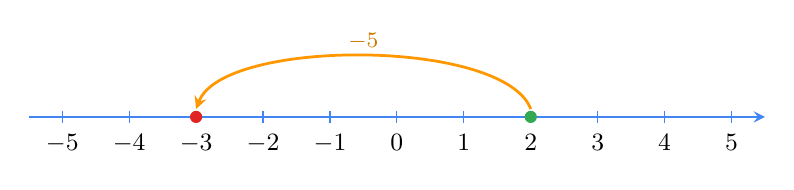
\begin{tikzpicture}[x=0.85cm,>=stealth]
\draw[->,thick,Navy] (-5.5,0)--(5.5,0);
\foreach \i in {-5,...,5}{\draw[Navy] (\i,0.08)--(\i,-0.08); \node[below,font=\small] at (\i,-0.1){$\i$};}
\fill[tmGreen] (2,0) circle (2.2pt); \fill[AnsRed] (-3,0) circle (2.2pt);
% cung "-5": bắt đầu đúng tại 2, mũi tên kết thúc đúng tại -3 (đỉnh cung ở x=-0.5, y=0.775)
\draw[->,tmOrange,line width=1pt] (2,0.1) .. controls (1.6,1.0) and (-2.6,1.0) .. (-3,0.1);
\node[above,font=\footnotesize,text=tmOrange!80!black,inner sep=2pt] at (-0.5,0.775){$-5$};
\end{tikzpicture}\end{center}
\emph{Ví dụ:} $2+(-5)=-3$: từ $2$, đi sang trái $5$ bước, đến $-3$.

\textbf{2. Cộng, trừ số nguyên.}
\begin{itemize}[leftmargin=1.4em,itemsep=1pt,topsep=2pt]
\item Cộng hai số cùng dấu: cộng phần số, giữ dấu chung: $(-11)+(-26)=-37$.
\item Cộng hai số khác dấu: lấy phần số lớn trừ phần số nhỏ, lấy dấu của số có phần số lớn hơn: $11+(-37)=-26$.
\item Trừ là cộng với số đối: $a-b=a+(-b)$. Ví dụ: $-26-11=-26+(-11)=-37$.
\end{itemize}

\textbf{3. Thứ tự thực hiện phép tính.} Ngoặc trước $\to$ luỹ thừa $\to$ nhân, chia (từ trái sang phải)
$\to$ cộng, trừ (từ trái sang phải). Ví dụ: $6+2\cdot 3=6+6=12$ (không phải $8\cdot 3$).

\textbf{4. Tính chất phân phối.} $a(b+c)=ab+ac$ và $a(b-c)=ab-ac$.
\emph{Ví dụ:} $3(T+4)=3T+12$;\quad $20\cdot 3-20\cdot 2{,}25=20\cdot(3-2{,}25)=20\cdot 0{,}75=15$.

\textbf{5. Thu gọn biểu thức.} Cộng các số hạng ``cùng loại'': $3x+5x=8x$; \
$(a+1)+(b+1)+(c+1)+(d+1)=(a+b+c+d)+4$.

\textbf{6. Điểm trên mặt phẳng toạ độ.} Điểm $(x;y)$ có hoành độ $x$ và tung độ $y$. Đi sang phải $k$
đơn vị thì $x$ tăng $k$; đi lên $k$ đơn vị thì $y$ tăng $k$ (đi sang trái, đi xuống thì giảm).
\end{knowbox}

\begin{proofbox}
\textbf{Vì sao $a(b+c)=ab+ac$?} Xét một hình chữ nhật có chiều rộng $a$, chiều dài $b+c$. Diện tích của nó là
$a(b+c)$. Nhưng ta cũng có thể cắt nó thành hai hình chữ nhật nhỏ có diện tích $ab$ và $ac$. Cùng một
diện tích nên $a(b+c)=ab+ac$.
\begin{figC}
\fill[tmBlue!18] (0,0) rectangle (3,1.2); \fill[tmGreen!20] (3,0) rectangle (5,1.2);
\draw[Navy,line width=0.9pt] (0,0) rectangle (5,1.2); \draw[Navy,line width=0.9pt] (3,0)--(3,1.2);
\node at (1.5,0.6){$ab$}; \node at (4,0.6){$ac$};
\node[left] at (0,0.6){$a$}; \node[below] at (1.5,0){$b$}; \node[below] at (4,0){$c$};
\end{figC}
\end{proofbox}

\begin{warnbox}
$3(T+4)$ \emph{không bằng} $3T+4$: phải nhân $3$ với \emph{từng} số hạng trong ngoặc, $3(T+4)=3T+3\cdot 4=3T+12$.
Tương tự $-(a-b)=-a+b$ (đổi dấu \emph{mọi} số hạng trong ngoặc).
\end{warnbox}

% ------------------------------------------------------------------------------------------
\needspace{6\baselineskip}\shead{Đẳng thức, phương trình và nguyên tắc cân bằng}
\begin{knowbox}
\textbf{1. Phương trình.} Một đẳng thức chứa ẩn, chẳng hạn $2(x+8)=38$, gọi là \textbf{phương trình}.
Số thay vào ẩn làm cho hai vế bằng nhau gọi là \textbf{nghiệm}. \emph{Giải phương trình} là tìm nghiệm.

\textbf{2. Nguyên tắc cân bằng.} Hãy tưởng tượng phương trình là một chiếc cân đang thăng bằng.
Cân vẫn thăng bằng nếu ta:
\begin{itemize}[leftmargin=1.4em,itemsep=1pt,topsep=2pt]
\item cộng (hoặc trừ) \emph{cùng một số} vào cả hai vế;
\item nhân (hoặc chia) cả hai vế với \emph{cùng một số khác $0$}.
\end{itemize}
Hệ quả quen thuộc là \textbf{quy tắc chuyển vế}: chuyển một số hạng từ vế này sang vế kia thì phải \emph{đổi dấu} số hạng đó.

\begin{center}
\rvaaScale{\rvaaSq\,\rvaaSq\enspace\rvaaWt{3 kg}}{\rvaaWt{11 kg}}
\end{center}
\emph{Ví dụ:} hai hộp như nhau cùng quả cân $3$ kg cân bằng với $11$ kg: $2x+3=11$.
Bỏ quả cân $3$ kg ở cả hai đĩa: $2x=11-3=8$. Chia đôi cả hai đĩa: $x=8:2=4$. Mỗi hộp nặng $4$ kg.

\textbf{3. Phép thế trên cân.} Nếu một đĩa cân chứa $A$ cân bằng với $B$ thì ở bất kì chiếc cân nào khác, ta có thể
thay $A$ bằng $B$ mà cân vẫn thăng bằng (giống như thay một biểu thức bằng một biểu thức bằng nó).

\textbf{4. Luôn thử lại.} Sau khi giải, thay nghiệm vào phương trình ban đầu để chắc chắn hai vế bằng nhau.
\end{knowbox}

\begin{proofbox}
\textbf{Vì sao chuyển vế phải đổi dấu?} Từ $2x+3=11$, trừ $3$ ở cả hai vế (cân vẫn thăng bằng):
$2x+3-3=11-3$, tức là $2x=11-3$. Nhìn kết quả, ta thấy số hạng $+3$ ở vế trái như đã ``nhảy'' sang vế phải và trở thành $-3$.
Thật ra không có gì ``nhảy'' cả, ta chỉ trừ cùng một số ở hai vế.
\end{proofbox}

\begin{warnbox}
Quên đổi dấu khi chuyển vế: từ $x+11=-26$ mà viết $x=-26+11$ là \textbf{sai}. Đúng là $x=-26-11=-37$.
\end{warnbox}

\begin{tipbox}
Gặp bài trắc nghiệm có phương trình, ta có thể \emph{thay lần lượt từng phương án} vào phương trình. Cách này
chậm hơn nhưng rất chắc chắn, và cũng là cách thử lại tốt nhất.
\end{tipbox}

% ------------------------------------------------------------------------------------------
\needspace{6\baselineskip}\shead{Giải bài toán bằng cách lập phương trình}
\begin{knowbox}
\textbf{Bốn bước giải bài toán có lời văn.}
\begin{enumerate}[leftmargin=1.6em,itemsep=1pt,topsep=2pt]
\item \textbf{Chọn ẩn}: gọi đại lượng cần tìm (hoặc một đại lượng liên quan) là $x$; ghi rõ đơn vị và điều kiện (ví dụ $x>0$, $x$ là số nguyên).
\item \textbf{Biểu diễn} các đại lượng khác theo $x$.
\item \textbf{Lập phương trình} từ điều kiện của đề bài rồi \textbf{giải}.
\item \textbf{Đối chiếu} điều kiện, \textbf{thử lại} và \textbf{trả lời} đúng câu hỏi.
\end{enumerate}

\textbf{Các dạng hay gặp.}
\begin{itemize}[leftmargin=1.4em,itemsep=2pt,topsep=2pt]
\item \textbf{Số nguyên liên tiếp:} $n,\ n+1,\ n+2$ (hoặc gọn hơn $n-1,\ n,\ n+1$). Số chẵn (lẻ) liên tiếp hơn kém nhau $2$: $n,\ n+2,\ n+4$.
\item \textbf{Tổng từng đôi:} ba vật $a,b,c$ cân từng đôi được $a+b$, $b+c$, $c+a$. Cộng ba kết quả:
$(a+b)+(b+c)+(c+a)=2(a+b+c)$, nên \emph{tổng ba vật bằng nửa tổng các kết quả}. Muốn tìm một vật, lấy tổng ba vật trừ đi tổng hai vật kia.
\item \textbf{Góc trong tam giác:} tổng ba góc của một tam giác bằng $180^\circ$; tam giác cân có hai góc ở đáy bằng nhau.
\item \textbf{Trung bình:} giá trị trung bình $=$ tổng các giá trị $:$ số các giá trị; giá trung bình $=$ tổng số tiền $:$ tổng khối lượng.
\end{itemize}
\end{knowbox}

\needspace{10\baselineskip}\textbf{Hai ví dụ nhỏ.}

\emph{a) Tam giác cân có một góc $70^\circ$.} Góc $70^\circ$ có thể là \emph{góc ở đáy} hoặc \emph{góc ở đỉnh}, nên phải xét hai trường hợp:
\begin{itemize}[leftmargin=1.4em,itemsep=1pt,topsep=1pt]
\item Nếu $70^\circ$ là góc ở đáy: hai góc đáy là $70^\circ$ và $70^\circ$, góc ở đỉnh là $180^\circ-70^\circ-70^\circ=40^\circ$.
\item Nếu $70^\circ$ là góc ở đỉnh: hai góc đáy bằng nhau và có tổng $180^\circ-70^\circ=110^\circ$, mỗi góc là $55^\circ$.
\end{itemize}
\begin{figC}
\draw[tmBlue,line width=1pt,fill=tmBlue!8] (0,0)--(2.4,0)--(1.2,3.3)--cycle;
\node[font=\footnotesize] at (0.45,0.25){$70^\circ$}; \node[font=\footnotesize] at (1.95,0.25){$70^\circ$}; \node[font=\footnotesize] at (1.2,2.35){$40^\circ$};
\draw[tmOrange!85!black,line width=1pt,fill=tmOrange!10] (4,0)--(7.4,0)--(5.7,2.43)--cycle;
\node[font=\footnotesize] at (4.55,0.22){$55^\circ$}; \node[font=\footnotesize] at (6.85,0.22){$55^\circ$}; \node[font=\footnotesize] at (5.7,1.85){$70^\circ$};
\end{figC}

\emph{b) Giá trung bình.} Mua $300$ g kẹo loại I hết $\$3$ và $200$ g kẹo loại II hết $\$4$. Giá trung bình của
$100$ g kẹo là $(3+4):(300+200)\cdot 100=7:500\cdot 100=1{,}4$, tức là $\$1{,}40$.
\emph{Không} được lấy trung bình của hai giá $\$1$ và $\$2$ cho mỗi $100$ g (sẽ ra $\$1{,}50$, sai), vì hai loại kẹo được mua với khối lượng khác nhau.

\begin{proofbox}
\textbf{Ba số nguyên liên tiếp: số ở giữa bằng tổng chia $3$.} Gọi ba số là $n-1$, $n$, $n+1$. Tổng của chúng là
$(n-1)+n+(n+1)=3n$ (vì $-1$ và $+1$ triệt tiêu). Vậy số ở giữa $n=\text{tổng}:3$. Chẳng hạn tổng là $153$ thì số giữa là $51$ và ba số là $50,51,52$.
\end{proofbox}

\begin{tipbox}
Đặt ẩn là \emph{số ở giữa} thường làm phương trình gọn nhất. Với các bài ``tổng từng đôi'', đừng vội đặt ba ẩn và giải hệ:
hãy \emph{cộng tất cả lại} trước.
\end{tipbox}

\begin{warnbox}
Giải xong phương trình chưa phải là xong bài! Phải đọc lại câu hỏi: đề hỏi số \emph{lớn nhất}, vật \emph{nhẹ nhất}, hay \emph{tổng}...?
Rất nhiều bạn tìm đúng $x$ nhưng chọn sai đáp án vì trả lời nhầm câu hỏi.
\end{warnbox}

\needspace{5\baselineskip}
\begin{parentbox}
Khi con bí, hãy hỏi: ``Cái gì mình chưa biết? Gọi nó là $x$ nhé. Bây giờ, đề bài nói gì về $x$?''
Hãy để con nói thành lời trước, rồi mới viết thành phương trình.
\end{parentbox}

% ------------------------------------------------------------------------------------------
\needspace{6\baselineskip}\shead{Quy luật, bảng giá trị và dãy số cách đều}
\begin{knowbox}
\textbf{1. Dãy số cách đều.} Một dãy số mà hai số liền nhau luôn hơn kém nhau cùng một số $d$ (gọi là
\textbf{khoảng cách} hay \textbf{công sai}) được gọi là dãy cách đều. Nếu số hạng đầu là $a$ thì
\[\text{số hạng thứ } n \;=\; a+(n-1)\cdot d .\]
\emph{Ví dụ:} dãy $7,10,13,16,\dots$ có $a=7$, $d=3$; số hạng thứ $n$ là $7+3(n-1)=3n+4$.

\textbf{2. Từ bảng giá trị đến biểu thức.} Khi $n$ tăng $1$ mà giá trị luôn tăng $d$, biểu thức có dạng
$d\cdot n+\text{(một số)}$. Tìm ``một số'' bằng cách thay $n=1$.
\begin{center}
\begin{tabular}{|c|c|c|c|c|c|}
\hline
\rowcolor{tmBlue!10} $n$ & $1$ & $2$ & $3$ & $4$ & $5$\\ \hline
giá trị & $4$ & $7$ & $10$ & $13$ & $16$\\ \hline
\end{tabular}
\end{center}
Mỗi lần $n$ tăng $1$, giá trị tăng $3$ nên biểu thức có dạng $3n+b$. Thay $n=1$: $3+b=4$, suy ra $b=1$. Vậy giá trị $=3n+1$.

\textbf{3. Một số có nằm trong dãy không?} Số $N$ thuộc dãy $a,\ a+d,\ a+2d,\dots$ khi và chỉ khi
$N-a$ chia hết cho $d$ (và $N\ge a$). Với dãy đếm lùi $a,\ a-d,\ a-2d,\dots$ thì xét $a-N$.

\textbf{4. Số chung của hai dãy; hiện tượng lặp lại.} Nếu hai dãy cách đều có khoảng cách $d_1$, $d_2$ có một số chung thì
các số chung cách nhau đúng $\text{BCNN}(d_1,d_2)$. Tương tự, những sự việc lặp lại sau $p$ phút và sau $q$ phút sẽ
cùng xảy ra lại sau mỗi $\text{BCNN}(p,q)$ phút.
\end{knowbox}

\begin{tipbox}
\emph{Ví dụ về sự lặp lại.} Xe buýt thứ nhất cứ $12$ phút lại về bến, xe thứ hai cứ $20$ phút lại về bến. Lúc $7\,h$ cả hai cùng ở bến.
Thời điểm xe thứ nhất về bến: sau $12, 24, 36, 48, \mathbf{60},\dots$ phút; xe thứ hai: sau $20, 40, \mathbf{60},\dots$ phút.
Hai xe lại gặp nhau ở bến sau mỗi $\text{BCNN}(12,20)=60$ phút, tức lúc $8\,h$, $9\,h$, \dots

Tương tự, hai dãy $7,10,13,\dots$ (cách $3$) và $2026,2021,2016,\dots$ (cách $5$) nếu có số chung thì các số chung cách nhau $\text{BCNN}(3,5)=15$.
\end{tipbox}

\begin{proofbox}
\textbf{Vì sao số hạng thứ $n$ là $a+(n-1)d$?} Đi từ số hạng thứ $1$ đến số hạng thứ $n$, ta bước qua $n-1$ ``khoảng'',
mỗi khoảng cộng thêm $d$. Giống như đi từ cột điện thứ $1$ đến cột thứ $5$ chỉ qua $4$ khoảng.
\begin{figC}
\foreach \i/\v in {0/a,1/a+d,2/a+2d,3/a+3d}{\fill[tmBlue] (2.2*\i,0) circle (2.5pt); \node[below,font=\footnotesize] at (2.2*\i,-0.1){$\v$};}
\foreach \i in {0,1,2}{\draw[->,tmOrange,line width=0.9pt] (2.2*\i,0.1) to[out=60,in=120] node[above,font=\footnotesize]{$+d$} (2.2*\i+2.2,0.1);}
\node[font=\footnotesize,text=Slate] at (0,-0.75){(thứ 1)}; \node[font=\footnotesize,text=Slate] at (6.6,-0.75){(thứ 4)};
\end{figC}
Từ số thứ $1$ đến số thứ $4$ có $3$ bước $+d$, nên số thứ $4$ là $a+3d$.
\end{proofbox}

\begin{warnbox}
Kiểm tra một công thức chỉ với \emph{một} cột của bảng là chưa đủ. Chẳng hạn bảng $1,3,5,7,9$: cả $3n-2$ lẫn $2n-1$ đều
cho giá trị $1$ khi $n=1$, nhưng với $n=2$ thì $3n-2=4\neq 3$. Hãy thử với \emph{ít nhất hai, ba cột}.
\end{warnbox}

% ------------------------------------------------------------------------------------------
\needspace{6\baselineskip}\shead{Tỉ lệ, đơn vị đo và chuyển động đều}
\begin{knowbox}
\textbf{1. Đại lượng tỉ lệ thuận.} Nếu một thìa thức ăn đủ cho $8$ con cá thì $2$ thìa đủ cho $16$ con, $4$ thìa đủ cho $32$ con:
gấp số thìa lên bao nhiêu lần thì số cá cũng gấp lên bấy nhiêu lần. Ta nói $y$ \textbf{tỉ lệ thuận} với $x$ theo hệ số $k$ nếu $y=k\cdot x$.
Cách giải quen thuộc: \textbf{rút về đơn vị} (tính cho $1$ phần trước, rồi nhân lên).

\textbf{2. Chuyển động đều.} Với $s$ là quãng đường, $v$ là vận tốc, $t$ là thời gian:
\[ s=v\cdot t,\qquad t=\frac{s}{v},\qquad v=\frac{s}{t}.\]
Nhớ dùng đơn vị phù hợp: $v$ tính bằng km/h thì $s$ tính bằng km và $t$ tính bằng giờ.

Hai người chạy \emph{cùng một khoảng thời gian}: ai nhanh gấp $k$ lần thì đi được quãng đường gấp $k$ lần.

\emph{Chạy ngược chiều trên đường tròn:} từ lần gặp nhau này đến lần gặp nhau sau, \emph{tổng} quãng đường hai người chạy được đúng bằng một vòng.
Nếu người thứ nhất nhanh gấp $k$ lần người thứ hai thì trong mỗi lượt đó, người thứ nhất chạy $\dfrac{k}{k+1}$ vòng, người thứ hai chạy $\dfrac{1}{k+1}$ vòng.

\textbf{3. Đổi đơn vị thời gian.}
$1$ phút $=60$ giây;\ \ $1$ giờ $=60$ phút $=60\times 60=3\,600$ giây;\ \ $1$ ngày $=24$ giờ;\ \ $1$ tuần $=7$ ngày.
Do đó $1$ tuần $=7\times 24$ giờ $=7\times 24\times 60$ phút $=7\times 24\times 60\times 60$ giây.

\textbf{4. Tiền.} Số tờ tiền $=$ tổng số tiền $:$ mệnh giá một tờ. \ Tiền chênh lệch sau $n$ lần
$=n\times(\text{giá lớn}-\text{giá nhỏ})$.
\end{knowbox}

\begin{tipbox}
Đọc một tích như $60\times 60\times 24\times 7$ như một \emph{chuỗi đổi đơn vị}, đọc từ phải sang trái:
$7$ (ngày trong một tuần) $\times 24$ (giờ trong một ngày) $\times 60$ (phút trong một giờ) $\times 60$ (giây trong một phút).
Kết quả là số giây trong một tuần.
\end{tipbox}

\begin{proofbox}
\textbf{Vì sao tính chênh lệch ``mỗi lần'' rồi nhân lên cũng được?} Theo tính chất phân phối:
$20\times 3-20\times 2{,}25=20\times(3-2{,}25)=20\times 0{,}75=15$. Hai cách tính luôn cho cùng một kết quả,
nhưng cách thứ hai nhẩm nhanh hơn nhiều.
\end{proofbox}

\begin{warnbox}
Trong bài chuyển động, đọc kĩ ``đã đi được bao nhiêu'' và ``còn lại bao nhiêu''. Đi được một nửa quãng đường $510$ km
thì quãng đường còn lại là $510:2=255$ km, không phải $510$ km.
\end{warnbox}

% ------------------------------------------------------------------------------------------
\needspace{6\baselineskip}\shead{Phân số bằng nhau và phân số của một số}
\begin{knowbox}
\textbf{1. Tính chất cơ bản.} Nhân (hoặc chia) cả tử và mẫu của một phân số với cùng một số khác $0$,
ta được một phân số bằng nó: $\dfrac{3}{7}=\dfrac{3\cdot 9}{7\cdot 9}=\dfrac{27}{63}$.

\textbf{2. Nhận biết hai phân số bằng nhau.} Với $b\neq 0$, $d\neq 0$:\quad
$\dfrac{a}{b}=\dfrac{c}{d}$ khi và chỉ khi $a\cdot d=b\cdot c$ (``nhân chéo'').

\textbf{3. Hai phân số cùng tử.} Nếu $\dfrac{1}{p}=\dfrac{1}{q}$ (hay $\dfrac{m}{p}=\dfrac{m}{q}$ với $m\neq 0$) thì $p=q$.
Hai phân số có tử bằng nhau và bằng nhau thì mẫu cũng bằng nhau.

\textbf{4. Phân số của một số.} Muốn tìm $\dfrac{m}{n}$ của số $A$, ta tính $A\cdot\dfrac{m}{n}=A:n\cdot m$.
\emph{Ví dụ:} $\dfrac{3}{7}$ của $168$ km là $168:7\cdot 3=24\cdot 3=72$ km. Phần còn lại ứng với $1-\dfrac{3}{7}=\dfrac{4}{7}$.
\end{knowbox}

\begin{proofbox}
\textbf{Vì sao $\dfrac{1}{p}=\dfrac{1}{q}$ kéo theo $p=q$?} Nhân chéo: $1\cdot q=p\cdot 1$, tức là $q=p$.
Nói cách khác: chia một chiếc bánh thành $p$ phần và thành $q$ phần mà mỗi phần to bằng nhau thì số phần phải như nhau.
\end{proofbox}

% ------------------------------------------------------------------------------------------
\needspace{6\baselineskip}\shead{So sánh và suy luận về thứ tự}
\begin{knowbox}
\textbf{1. Tính chất bắc cầu.} Nếu $a<b$ và $b<c$ thì $a<c$. Nhờ đó ta có thể xếp nhiều số thành một hàng: $a<b<c<d$.

\textbf{2. Kĩ thuật ``đặt bằng $k$''.} Khi nhiều biểu thức bằng nhau, ví dụ $a-2=b+2=c+1=d-3$, hãy gọi giá trị chung là $k$:
\[a=k+2,\qquad b=k-2,\qquad c=k-1,\qquad d=k+3.\]
Bây giờ mọi số được so sánh với cùng một mốc $k$; xếp các ``phần thêm'' $-2<-1<+2<+3$ ta được $b<c<a<d$.
\begin{center}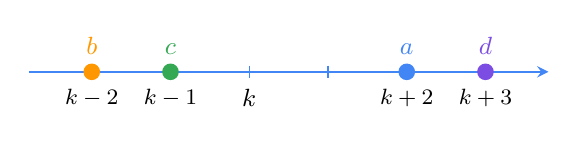
\begin{tikzpicture}[x=1cm,>=stealth]
\draw[->,thick,Navy] (-2.8,0)--(3.8,0);
\foreach \i in {-2,...,3}{\draw[Navy] (\i,0.08)--(\i,-0.08);}
\node[below,font=\small] at (0,-0.1){$k$};
\foreach \i/\l/\c in {-2/b/tmOrange,-1/c/tmGreen,2/a/tmBlue,3/d/tmPurple}{\fill[\c] (\i,0) circle (3pt); \node[above,font=\small\bfseries,text=\c] at (\i,0.1){$\l$};}
\node[below,font=\footnotesize] at (-2,-0.1){$k-2$}; \node[below,font=\footnotesize] at (-1,-0.1){$k-1$};
\node[below,font=\footnotesize] at (2,-0.1){$k+2$}; \node[below,font=\footnotesize] at (3,-0.1){$k+3$};
\end{tikzpicture}\end{center}

\textbf{3. Suy luận logic về thứ tự.} Với các câu như ``Anna có nhiều mèo hơn Ben'', hãy dịch thành kí hiệu ($A>B$),
viết tất cả các điều kiện ra rồi nối chúng bằng tính chất bắc cầu. Một khẳng định ``\emph{chắc chắn đúng}'' phải đúng trong
\emph{mọi} trường hợp thoả mãn đề bài; chỉ cần một ví dụ trái ngược là đủ để bác bỏ nó.
\end{knowbox}

\begin{tipbox}
\emph{Ví dụ suy luận.} Anna cao hơn Ben; Chloe thấp hơn Ben; David cao hơn Chloe. Ai thấp nhất?
Viết kí hiệu (mỗi chữ là chiều cao của một bạn): $A>B$, \ $B>C$, \ $D>C$. Từ $A>B>C$ và $D>C$ ta thấy cả $A$, $B$, $D$ đều lớn hơn $C$: \textbf{Chloe thấp nhất}.
Nhưng ta \emph{không} biết David cao hơn hay thấp hơn Anna (chẳng hạn Anna $1{,}6$ m, Ben $1{,}5$ m, Chloe $1{,}2$ m thì David cao $1{,}7$ m hay $1{,}3$ m đều thoả mãn mọi điều kiện), nên câu ``David cao nhất'' \emph{không chắc chắn} đúng.
\end{tipbox}

\begin{warnbox}
Nhìn thấy $a-2$ và $b+2$ bằng nhau, nhiều bạn vội kết luận ``$a$ bé hơn vì bị trừ''. Ngược lại mới đúng: $a$ phải \emph{bớt đi} $2$
mới bằng $b$ \emph{thêm} $2$, nên $a$ lớn hơn $b$ đúng $4$ đơn vị.
\end{warnbox}

\begin{parentbox}
Hãy dùng đồ vật thật: ``Túi của con bớt $2$ viên bi thì bằng túi của mẹ thêm $2$ viên. Túi nào nhiều hơn?''
Cho con dùng bi để kiểm tra. Hình ảnh cụ thể giúp con không bị đánh lừa bởi dấu cộng, dấu trừ.
\end{parentbox}

% ==========================================================================================
\needspace{6\baselineskip}\shead{Ví dụ mẫu}

\begin{exbox}{Ví dụ 1 \ (Dịch lời văn và tính giá trị biểu thức)}
\textbf{a)} Tính giá trị của biểu thức $A=2x^2-3x+1$ tại $x=-2$.

\textbf{b)} Bạn Emma đang có $\$50$ trong ống tiết kiệm. Mỗi tuần Emma bỏ thêm vào $\$20$.
Viết biểu thức biểu thị số tiền (tính bằng đô la) trong ống tiết kiệm sau $t$ tuần, rồi tính số tiền đó sau $6$ tuần.
\guide
\step{1}{Câu a: thay $x=-2$, nhớ đặt trong ngoặc}
\[A=2\cdot(-2)^2-3\cdot(-2)+1.\]
\step{2}{Tính theo thứ tự: luỹ thừa $\to$ nhân $\to$ cộng, trừ}
$(-2)^2=(-2)\cdot(-2)=4$, nên $2\cdot 4=8$. \ $3\cdot(-2)=-6$, nên $-3\cdot(-2)=+6$. Vậy $A=8+6+1=15$.
\step{3}{Câu b: tìm quy luật bằng một bảng nhỏ}
\begin{center}
\begin{tabular}{|c|c|c|c|c|}
\hline
\rowcolor{tmBlue!10} Số tuần & $0$ & $1$ & $2$ & $t$\\ \hline
Số tiền (đô la) & $50$ & $50+20$ & $50+2\cdot 20$ & $50+20t$\\ \hline
\end{tabular}
\end{center}
Số tiền có sẵn không đổi; phần bỏ thêm bằng $20$ nhân với số tuần. Biểu thức: $50+20t$ (đô la).
\step{4}{Thay $t=6$}
$50+20\cdot 6=50+120=170$ (đô la).
\begin{warnbox}Không viết $(50+20)\cdot t$: số tiền ban đầu chỉ có \emph{một lần}, không được nhân với số tuần.\end{warnbox}
\ans{a) $A=15$;\ \ b) $50+20t$ (đô la); sau $6$ tuần có $\$170$.}
\end{exbox}

\begin{exbox}{Ví dụ 2 \ (Giải phương trình bằng nguyên tắc cân bằng)}
Giải các phương trình:\quad \textbf{a)} $5x-7=2x+11$;\qquad \textbf{b)} $\dfrac{x}{12}=\dfrac{5}{4}$.
\guide
\step{1}{Câu a: gom các số hạng chứa $x$ về vế trái}
Trừ $2x$ ở cả hai vế: $5x-2x-7=11$, tức là $3x-7=11$.
\step{2}{Gom các số về vế phải}
Cộng $7$ vào cả hai vế: $3x=11+7=18$.
\step{3}{Chia cả hai vế cho $3$}
$x=18:3=6$.
\verify{Vế trái: $5\cdot 6-7=30-7=23$. Vế phải: $2\cdot 6+11=12+11=23$. Hai vế bằng nhau.}
\step{4}{Câu b: quy về cùng mẫu (hoặc nhân chéo)}
Ta có $\dfrac{5}{4}=\dfrac{5\cdot 3}{4\cdot 3}=\dfrac{15}{12}$. Hai phân số $\dfrac{x}{12}$ và $\dfrac{15}{12}$ có cùng mẫu
và bằng nhau nên $x=15$. (Nhân chéo cũng được: $4x=12\cdot 5=60$, $x=60:4=15$.)
\begin{recallbox}$\dfrac{a}{b}=\dfrac{c}{d}$ khi và chỉ khi $ad=bc$ ($b,d\neq 0$).\end{recallbox}
\ans{a) $x=6$;\ \ b) $x=15$.}
\end{exbox}

\begin{exbox}{Ví dụ 3 \ (Số chẵn liên tiếp)}
Tổng của bốn số chẵn liên tiếp bằng $116$. Tìm số lớn nhất trong bốn số đó.
\guide
\step{1}{Chọn ẩn}
Gọi số chẵn bé nhất là $n$ ($n$ là số chẵn). Hai số chẵn liên tiếp hơn kém nhau $2$, nên bốn số là
$n,\ n+2,\ n+4,\ n+6$.
\step{2}{Lập phương trình}
$n+(n+2)+(n+4)+(n+6)=116$, tức là $4n+12=116$.
\step{3}{Giải}
$4n=116-12=104$, \ $n=104:4=26$. Bốn số là $26,\ 28,\ 30,\ 32$.
\verify{$26+28+30+32=116$. Đúng.}
\step{4}{Trả lời đúng câu hỏi}
Đề hỏi số \emph{lớn nhất}: đó là $32$.
\begin{tipbox}Cách nhẩm: bốn số cách đều nên trung bình của chúng là $116:4=29$, nằm chính giữa hai số giữa $28$ và $30$. Từ đó suy ra ngay bốn số.\end{tipbox}
\ans{$32$}
\end{exbox}

\begin{exbox}{Ví dụ 4 \ (Cân từng đôi)}
Ba bạn Anna, Ben, Chloe lần lượt đứng lên cân từng đôi một. Anna và Ben nặng $72$ kg; Anna và Chloe nặng $78$ kg;
Ben và Chloe nặng $80$ kg. Mỗi bạn nặng bao nhiêu ki-lô-gam?
\guide
\step{1}{Chọn ẩn và biểu diễn các đại lượng theo ẩn}
Gọi khối lượng của Anna là $x$ (kg), $x>0$.
Vì Anna và Ben nặng $72$ kg nên Ben nặng $72-x$ (kg).
Vì Anna và Chloe nặng $78$ kg nên Chloe nặng $78-x$ (kg).
\step{2}{Lập phương trình từ lần cân thứ ba}
Ben và Chloe nặng $80$ kg, nên
\[(72-x)+(78-x)=80.\]
\step{3}{Giải phương trình}
Thu gọn vế trái: $72+78-x-x=150-2x$, nên $150-2x=80$. Chuyển vế: $2x=150-80=70$, suy ra $x=70:2=35$.
\step{4}{Tính khối lượng hai bạn còn lại}
Anna nặng $35$ kg;\quad Ben nặng $72-35=37$ (kg);\quad Chloe nặng $78-35=43$ (kg).
\begin{tipbox}\textbf{Cách 2.} Gọi khối lượng ba bạn là $a$, $b$, $c$ (kg). Cộng vế theo vế $a+b=72$, $a+c=78$, $b+c=80$ (mỗi chữ xuất hiện hai lần): $2(a+b+c)=230$, nên $a+b+c=115$. Suy ra $c=115-72=43$, $b=115-78=37$, $a=115-80=35$.\end{tipbox}
\verify{$35+37=72$, \ $35+43=78$, \ $37+43=80$. Cả ba lần cân đều khớp.}
\ans{Anna $35$ kg, Ben $37$ kg, Chloe $43$ kg.}
\end{exbox}

\begin{exbox}{Ví dụ 5 \ (Dãy cách đều)}
Cho dãy số $4,\ 7,\ 10,\ 13,\ \dots$ (mỗi số hơn số liền trước $3$ đơn vị).
\textbf{a)} Viết biểu thức của số hạng thứ $n$.\quad \textbf{b)} Tính số hạng thứ $50$.\quad
\textbf{c)} Số $2026$ có thuộc dãy không? Nếu có, đó là số hạng thứ mấy?
\guide
\step{1}{Số hạng thứ $n$}
Số hạng đầu $a=4$, khoảng cách $d=3$: số hạng thứ $n$ là $4+3(n-1)=4+3n-3=3n+1$.
\begin{recallbox}Số hạng thứ $n$ của dãy cách đều $=a+(n-1)d$.\end{recallbox}
\step{2}{Số hạng thứ $50$}
$3\cdot 50+1=151$.
\step{3}{Kiểm tra số $2026$}
Ta cần một số tự nhiên $n$ sao cho $3n+1=2026$, tức là $3n=2025$. Vì $2025:3=675$ (chia hết), nên $n=675$.
\verify{$3\cdot 675+1=2025+1=2026$. Đúng.}
\begin{warnbox}Đừng quên kiểm tra phép chia có chia hết hay không. Chẳng hạn $2027$ \emph{không} thuộc dãy vì $2026$ không chia hết cho $3$.\end{warnbox}
\ans{a) $3n+1$;\ \ b) $151$;\ \ c) có, là số hạng thứ $675$.}
\end{exbox}

\begin{exbox}{Ví dụ 6 \ (Chuyển động, phân số và đổi đơn vị)}
Một đoàn tàu chạy đều với vận tốc $72$ km/h trên quãng đường dài $360$ km. Tàu đã đi được $\dfrac{2}{3}$ quãng đường.
Hỏi tàu cần chạy thêm bao lâu nữa (tính ra giờ và phút) thì đến nơi?
\guide
\step{1}{Quãng đường đã đi}
$\dfrac{2}{3}$ của $360$ km là $360:3\cdot 2=120\cdot 2=240$ km.
\step{2}{Quãng đường còn lại}
$360-240=120$ km. (Hoặc: phần còn lại là $1-\dfrac{2}{3}=\dfrac{1}{3}$ quãng đường, $360:3=120$ km.)
\step{3}{Thời gian còn lại}
\begin{recallbox}$s=v\cdot t$, nên $t=\dfrac{s}{v}$ (thời gian $=$ quãng đường $:$ vận tốc).\end{recallbox}
Gọi $t$ (giờ) là thời gian tàu còn phải chạy. Ta có $72\cdot t=120$, nên
$t=120:72=\dfrac{120}{72}=\dfrac{5}{3}$ giờ $=1\dfrac{2}{3}$ giờ.
\step{4}{Đổi ra giờ và phút}
$\dfrac{2}{3}$ giờ $=\dfrac{2}{3}\cdot 60=40$ phút. Vậy $t=1$ giờ $40$ phút.
\verify{Trong $1$ giờ $40$ phút $=\dfrac{5}{3}$ giờ, tàu đi được $72\cdot\dfrac{5}{3}=24\cdot 5=120$ km. Đúng bằng quãng đường còn lại.}
\ans{$1$ giờ $40$ phút.}
\end{exbox}

\needspace{14\baselineskip}
\begin{exbox}{Ví dụ 7 \ (Bài toán chiếc cân)}
Cả hai chiếc cân dưới đây đều thăng bằng. Các hình giống nhau thì nặng bằng nhau.
\begin{center}
\rvaaScale{\rvaaSq}{\rvaaTri\,\rvaaCir}\hspace{1.2cm}\rvaaScale{\rvaaSq\,\rvaaCir}{\rvaaTri\,\rvaaTri\,\rvaaTri}
\end{center}
Hỏi hai hình vuông \rvaaSq\,\rvaaSq\ cân bằng với bao nhiêu hình tròn \rvaaCir?
\guide
\step{1}{Viết mỗi chiếc cân thành một đẳng thức}
Kí hiệu $V$, $T$, $O$ là khối lượng hình vuông, tam giác, hình tròn. Cân 1: $V=T+O$. \ Cân 2: $V+O=3T$.
\step{2}{Thế cân 1 vào cân 2}
Ở cân 2, thay hình vuông bằng ``một tam giác và một tròn'' (cân 1 cho phép):
$T+O+O=3T$.
\step{3}{Bỏ bớt những thứ giống nhau ở hai đĩa}
Bỏ một tam giác ở mỗi đĩa: $O+O=T+T$, tức $2O=2T$, nên $O=T$: một hình tròn nặng bằng một tam giác.
\step{4}{Trả lời}
$V=T+O=O+O=2O$, nên $2V=4O$: hai hình vuông cân bằng với $4$ hình tròn.
\verify{Chọn thử $O=T=1$, $V=2$: cân 1: $2=1+1$; cân 2: $2+1=3$. Đúng cả hai.}
\ans{$4$ hình tròn.}
\end{exbox}

\needspace{24\baselineskip}
\begin{exbox}{Ví dụ 8 \ (Sắp thứ tự nhờ kĩ thuật ``đặt bằng $k$'')}
Các số nguyên dương $a$, $b$, $c$ (đều lớn hơn $5$) thoả mãn\quad
$\dfrac{2}{a+3}=\dfrac{2}{b-1}=\dfrac{2}{c+5}$. Hãy sắp xếp $a$, $b$, $c$ theo thứ tự tăng dần.
\guide
\step{1}{Phân số cùng tử bằng nhau thì mẫu bằng nhau}
Ba phân số có cùng tử là $2$ và bằng nhau, nên các mẫu bằng nhau: $a+3=b-1=c+5$.
\begin{recallbox}Nếu $\dfrac{m}{p}=\dfrac{m}{q}$ với $m\neq 0$ thì $p=q$.\end{recallbox}
\step{2}{Đặt giá trị chung là $k$}
$a+3=k\Rightarrow a=k-3$;\quad $b-1=k\Rightarrow b=k+1$;\quad $c+5=k\Rightarrow c=k-5$.
\step{3}{So sánh với mốc $k$}
$k-5<k-3<k+1$, nên $c<a<b$.
\verify{Chọn $k=12$: $a=9$, $b=13$, $c=7$. Khi đó $\dfrac{2}{12}=\dfrac{2}{12}=\dfrac{2}{12}$ và quả thật $7<9<13$.}
\ans{$c<a<b$.}
\end{exbox}

% ==========================================================================================
\clearpage
\dividerbar{Luyện tập cơ bản}

% ---------------------------------------------------------------- Bài 1
\begin{probbox}{1}{\relax}
Cô Carrie lái ô tô chạy đều với vận tốc $85$ km/h trên một chuyến đi dài $510$ km. Hiện cô đã đi được đúng
một nửa quãng đường. Hỏi cô cần đi thêm bao nhiêu giờ nữa thì hết quãng đường?
\choices{$5$ giờ}{$425$ giờ}{$12$ giờ}{$1{,}5$ giờ}{$3$ giờ}
\end{probbox}
\probsol{
\textbf{Phân tích đề.} \emph{Đã biết:} vận tốc $85$ km/h (không đổi), cả quãng đường $510$ km, đã đi được một nửa.
\emph{Cần tìm:} thời gian để đi nốt phần còn lại.
\step{1}{Tính quãng đường còn lại}
Đã đi được một nửa thì còn lại cũng đúng một nửa: $510:2=255$ (km).
\step{2}{Gọi ẩn và lập phương trình}
\begin{recallbox}Quãng đường $=$ vận tốc $\times$ thời gian ($s=v\cdot t$), nên thời gian $=$ quãng đường $:$ vận tốc ($t=\dfrac{s}{v}$).\end{recallbox}
Gọi $t$ (giờ) là thời gian cô Carrie còn phải đi ($t>0$). Trong $t$ giờ, với vận tốc $85$ km/h, cô đi được $85t$ km.
Quãng đường này phải bằng quãng đường còn lại: $85t=255$.
\step{3}{Giải phương trình}
Chia cả hai vế cho $85$: $t=255:85=3$ (giờ). (Nhẩm: $85\times 3=255$.)
\begin{warnbox}Nếu lấy cả quãng đường $510:85=6$ giờ thì đó là thời gian của \emph{cả} chuyến đi, chưa trả lời đúng câu hỏi. Còn $510-85=425$ là phép tính vô nghĩa (trừ km cho km/h), đó là cái bẫy ở phương án (B).\end{warnbox}
\begin{tipbox}Cách khác: cả chuyến đi mất $510:85=6$ giờ; đã đi một nửa quãng đường (với vận tốc không đổi) tức là đã đi một nửa thời gian, nên còn $6:2=3$ giờ.\end{tipbox}
\verify{Trong $3$ giờ, ô tô đi được $85\times 3=255$ km, đúng bằng quãng đường còn lại.}
Kết quả $3$ giờ ứng với phương án \textbf{(E)}.
\ans{(E) $3$ giờ}
}

% ---------------------------------------------------------------- Bài 2

\begin{probbox}{2}{\relax}
Trong hình vẽ, tam giác có một cạnh dài $14$ cm và hai cạnh bằng nhau, mỗi cạnh dài $12$ cm; hình chữ nhật có chiều rộng
$8$ cm và chiều dài $x$ cm. Biết chu vi tam giác bằng chu vi hình chữ nhật. Tìm $x$.
\begin{figC}
% vẽ đúng tỉ lệ 0,2 cm : 1 cm: đáy 14 -> 2,8; cạnh bên 12 -> 2,4 (chiều cao 1,95); hình chữ nhật 11 x 8 -> 2,2 x 1,6
\begin{scope}[scale=0.85]
\draw[tmBlue,line width=1.1pt,fill=tmBlue!10] (0,4.05)--(2.8,4.05)--(1.4,2.1)--cycle;
\node[above] at (1.4,4.05){$14$ cm};
\node[anchor=west] at (2.3,3.15){$12$ cm};
\draw[tmBlue,line width=0.9pt] (0.6025,3.005)--(0.7975,3.145);
\draw[tmBlue,line width=0.9pt] (2.0025,3.145)--(2.1975,3.005);
\draw[tmOrange!85!black,line width=1.1pt,fill=tmOrange!12] (0.3,0)rectangle(2.5,1.6);
\node[right] at (2.5,0.8){$8$ cm};
\node[below] at (1.4,0){$x$ cm};
\end{scope}
\end{figC}
\choices{$8$}{$10$}{$11$}{$14$}{$15$}
\end{probbox}
\probsol{
\textbf{Phân tích đề.} Tam giác có ba cạnh $14$ cm, $12$ cm, $12$ cm (hai vạch nhỏ trên hình cho biết hai cạnh đó bằng nhau).
Hình chữ nhật có hai kích thước $x$ cm và $8$ cm. Hai chu vi bằng nhau. Cần tìm $x$.
\step{1}{Tính chu vi tam giác}
\begin{recallbox}Chu vi tam giác bằng tổng độ dài ba cạnh. Chu vi hình chữ nhật bằng $2\times(\text{dài}+\text{rộng})$.\end{recallbox}
Chu vi tam giác: $14+12+12=38$ (cm).
\begin{warnbox}Hình vẽ chỉ ghi số $12$ một lần, nhưng có \emph{hai} cạnh dài $12$ cm (có vạch đánh dấu bằng nhau). Nếu quên cạnh thứ ba, ta sẽ được $26$ cm và giải sai.\end{warnbox}
\step{2}{Lập phương trình}
Chu vi hình chữ nhật là $2(x+8)$. Cho hai chu vi bằng nhau: $2(x+8)=38$.
\step{3}{Giải phương trình}
Chia cả hai vế cho $2$: $x+8=19$. Trừ $8$ ở cả hai vế: $x=19-8=11$, ứng với phương án \textbf{(C)}.
\verify{Hình chữ nhật $11$ cm $\times$ $8$ cm có chu vi $11+8+11+8=38$ cm, đúng bằng chu vi tam giác.}
\begin{parentbox}Có thể minh hoạ bằng một sợi dây dài $38$ cm: uốn thành tam giác $14$ -- $12$ -- $12$, rồi uốn lại thành hình chữ nhật có cạnh $8$ cm. Con sẽ thấy ``chu vi'' chính là độ dài sợi dây, không đổi khi đổi hình.\end{parentbox}
\ans{(C) $11$}
}

% ---------------------------------------------------------------- Bài 3
\begin{probbox}{3}{\relax}
Cho $x=3$. Đẳng thức nào dưới đây đúng?
\choices{$2x=5$}{$3x-1=8$}{$x+5=3$}{$7-x=2$}{$6+2x=14$}
\end{probbox}
\probsol{
\textbf{Phân tích đề.} Ta thay $x=3$ vào vế trái của từng đẳng thức, tính ra số, rồi so sánh với vế phải. Chỉ có một đẳng thức đúng.
\begin{recallbox}Muốn tính giá trị của biểu thức, ta thay chữ bằng số rồi thực hiện phép tính theo thứ tự: nhân, chia trước; cộng, trừ sau.\end{recallbox}
\step{1}{Kiểm tra lần lượt từng phương án}
\begin{center}
\begin{tabular}{|c|l|c|c|}
\hline
\rowcolor{tmBlue!10} Phương án & Thay $x=3$ vào vế trái & Vế phải & Đúng/Sai\\ \hline
(A) & $2x=2\cdot 3=6$ & $5$ & Sai\\ \hline
(B) & $3x-1=3\cdot 3-1=9-1=8$ & $8$ & \textbf{Đúng}\\ \hline
(C) & $x+5=3+5=8$ & $3$ & Sai\\ \hline
(D) & $7-x=7-3=4$ & $2$ & Sai\\ \hline
(E) & $6+2x=6+2\cdot 3=6+6=12$ & $14$ & Sai\\ \hline
\end{tabular}
\end{center}
\begin{warnbox}Ở (E), nếu tính sai thứ tự là $(6+2)\cdot 3=24$ hoặc đọc $2x$ thành ``$23$'' thì sẽ bị nhầm. Nhân trước, cộng sau: $6+2\cdot 3=12$.\end{warnbox}
\step{2}{Kết luận}
Chỉ có đẳng thức ở (B) đúng: $3\cdot 3-1=8$. Vậy chọn \textbf{(B)}.
\ans{(B) $3x-1=8$}
}

% ---------------------------------------------------------------- Bài 4
\begin{probbox}{4}{\relax}
Tổng của ba số nguyên liên tiếp bằng $153$. Số lớn nhất trong ba số đó là
\choices{$52$}{$50$}{$53$}{$54$}{$51$}
\end{probbox}
\probsol{
\textbf{Phân tích đề.} Ba số nguyên liên tiếp là ba số đứng liền nhau trên trục số, hơn kém nhau $1$ (ví dụ $7,8,9$). Biết tổng là $153$. Cần tìm số \emph{lớn nhất}.
\step{1}{Chọn ẩn: gọi số ở giữa là $n$}
Ba số là $n-1$, \ $n$, \ $n+1$.
\step{2}{Lập phương trình}
$(n-1)+n+(n+1)=153$. Ở vế trái, $-1$ và $+1$ triệt tiêu nhau, còn lại $3n=153$.
\step{3}{Giải}
$n=153:3=51$. Ba số là $50$, $51$, $52$.
\begin{recallbox}Với ba số nguyên liên tiếp, số ở giữa bằng tổng chia cho $3$ (số ở giữa chính là trung bình cộng).\end{recallbox}
\begin{proofbox}Cách khác, gọi số bé nhất là $m$: $m+(m+1)+(m+2)=3m+3=153$, nên $3m=150$, $m=50$. Cùng ra ba số $50,51,52$.\end{proofbox}
\begin{tipbox}Mẹo trắc nghiệm: số lớn nhất phải lớn hơn trung bình $153:3=51$ một chút; thử ngay $50+51+52=153$.\end{tipbox}
\verify{$50+51+52=153$. Đúng.}
\step{4}{Trả lời đúng câu hỏi}
Số lớn nhất là $52$, ứng với phương án \textbf{(A)}.
\begin{warnbox}Phương án (E) $51$ là số \emph{ở giữa}, phương án (B) $50$ là số \emph{bé nhất}. Đọc kĩ câu hỏi để khỏi chọn nhầm.\end{warnbox}
\ans{(A) $52$}
}

% ---------------------------------------------------------------- Bài 5
\begin{probbox}{5}{\relax}
Mỗi thìa thức ăn cho cá đủ cho $8$ con cá vàng ăn. Hỏi $4$ thìa thức ăn như thế đủ cho bao nhiêu con cá vàng?
\choices{$12$}{$16$}{$8$}{$64$}{$32$}
\end{probbox}
\probsol{
\textbf{Phân tích đề.} $1$ thìa $\to$ $8$ con cá. Hỏi $4$ thìa $\to$ ? con cá.
Số thìa gấp lên bao nhiêu lần thì số cá được cho ăn cũng gấp lên bấy nhiêu lần (hai đại lượng tỉ lệ thuận).
\begin{recallbox}Nếu $y$ tỉ lệ thuận với $x$ theo hệ số $k$ thì $y=k\cdot x$. Ở đây $k=8$ (con cá cho mỗi thìa), nên số cá $=8\times$ số thìa.\end{recallbox}
\step{1}{Lập bảng hai đại lượng tỉ lệ thuận}
Gọi $y$ là số con cá được cho ăn khi dùng $x$ thìa thức ăn. Khi đó $y=8x$.
\begin{center}
\begin{tabular}{|c|c|c|c|c|}
\hline
\rowcolor{tmBlue!10} Số thìa $x$ & $1$ & $2$ & $3$ & $4$\\ \hline
Số cá $y=8x$ & $8$ & $16$ & $24$ & $?$\\ \hline
\end{tabular}
\end{center}
\step{2}{Thay $x=4$}
$y=8\cdot 4=32$ (con cá).
\begin{warnbox}Phương án (A) $12$ là $8+4$ (cộng thay vì nhân), phương án (D) $64$ là $8\times 8$. Mỗi thìa thêm vào cho \emph{thêm $8$ con}, nên phải nhân $8$ với số thìa.\end{warnbox}
\verify{$32:4=8$: mỗi thìa đúng $8$ con.}
Vậy chọn \textbf{(E)}.
\ans{(E) $32$}
}

% ---------------------------------------------------------------- Bài 6
\begin{probbox}{6}{\relax}
Cho $x=4$ và $y=3x$. Giá trị của $y$ là
\choices{$12$}{$24$}{$7$}{$81$}{$4$}
\end{probbox}
\probsol{
\textbf{Phân tích đề.} Biết $x=4$. Biểu thức $y=3x$ nghĩa là ``$y$ bằng $3$ nhân $x$''. Cần tính $y$.
\begin{recallbox}$3x$ là cách viết gọn của $3\cdot x$ (giữa số và chữ ta bỏ dấu nhân).\end{recallbox}
\step{1}{Thay $x=4$}
$y=3\cdot x=3\cdot 4=12$.
\begin{warnbox}Không được đọc $3x$ thành ``$34$'' (ghép chữ số), cũng không phải $3+4=7$ (phương án C) hay $3^4=81$ (phương án D).\end{warnbox}
\begin{tipbox}Có thể đọc $y=3x$ thành lời: ``$y$ gấp ba lần $x$''. Gấp ba lần $4$ là $12$.\end{tipbox}
\verify{$12:3=4=x$. Đúng.}
Vậy chọn \textbf{(A)}.
\ans{(A) $12$}
}

% ---------------------------------------------------------------- Bài 7
\begin{probbox}{7}{\relax}
Mỗi lần đi xe buýt, bạn Alex trả $\$2{,}25$, còn bạn Sam trả $\$3{,}00$ (hai bạn đi hai tuyến khác nhau).
Nếu mỗi bạn đi xe buýt $20$ lần thì tổng cộng Alex trả ít hơn Sam bao nhiêu tiền?
\choices{$\$25$}{$\$10$}{$\$15$}{$\$45$}{$\$60$}
\end{probbox}
\probsol{
\textbf{Phân tích đề.} Mỗi lần: Alex trả $\$2{,}25$, Sam trả $\$3{,}00$. Mỗi bạn đi $20$ lần. Hỏi \emph{số tiền chênh lệch} sau $20$ lần.
\step{1}{Cách 1 -- Tính tổng của từng bạn rồi trừ}
Alex trả: $20\times 2{,}25=45$ (đô la).\quad Sam trả: $20\times 3=60$ (đô la).\\
Chênh lệch: $60-45=15$ (đô la).
\step{2}{Cách 2 -- Tính chênh lệch mỗi lần rồi nhân lên (nhanh hơn)}
Mỗi lần Alex trả ít hơn Sam: $3{,}00-2{,}25=0{,}75$ (đô la).\\
Sau $20$ lần: $20\times 0{,}75=15$ (đô la).
\begin{recallbox}Tính chất phân phối: $20\times 3-20\times 2{,}25=20\times(3-2{,}25)$. Vì vậy hai cách luôn cho cùng kết quả.\end{recallbox}
\begin{warnbox}Phương án (D) $\$45$ là \emph{tổng số tiền của Alex}, phương án (E) $\$60$ là \emph{tổng số tiền của Sam}. Đề hỏi số tiền \emph{ít hơn}, tức là hiệu.\end{warnbox}
\verify{$45+15=60$. Đúng.}
Vậy chọn \textbf{(C)}.
\ans{(C) $\$15$}
}

% ---------------------------------------------------------------- Bài 8
\begin{probbox}{8}{\relax}
Biểu thức nào cho đúng các giá trị ở hàng thứ hai của bảng, ứng với mỗi giá trị $n$ ở hàng thứ nhất?
\begin{center}
\begin{tabular}{|c|c|c|c|c|c|}
\hline
\rowcolor{tmBlue!10} $n$ & $1$ & $2$ & $3$ & $4$ & $5$\\ \hline
Giá trị & $1$ & $3$ & $5$ & $7$ & $9$\\ \hline
\end{tabular}
\end{center}
\choices{$3n-2$}{$2(n-1)$}{$n+4$}{$2n$}{$2n-1$}
\end{probbox}
\probsol{
\textbf{Phân tích đề.} Ta cần một biểu thức chứa $n$ mà khi thay $n=1,2,3,4,5$ thì lần lượt được $1,3,5,7,9$.
\step{1}{Tìm quy luật của hàng giá trị}
Mỗi lần $n$ tăng thêm $1$ thì giá trị tăng thêm $2$ ($1\to 3\to 5\to 7\to 9$). Vậy biểu thức có dạng $2n+b$.
\begin{recallbox}Nếu $n$ tăng $1$ mà giá trị luôn tăng $d$ thì biểu thức có dạng $d\cdot n+b$; tìm $b$ bằng cách thay $n=1$.\end{recallbox}
\step{2}{Tìm $b$}
Thay $n=1$: $2\cdot 1+b=1$, suy ra $b=1-2=-1$. Biểu thức là $2n-1$.
\step{3}{Kiểm tra cả bảng và loại các phương án khác}
\begin{center}
\begin{tabular}{|c|c|c|c|c|c|c|}
\hline
\rowcolor{tmBlue!10} $n$ & $1$ & $2$ & $3$ & $4$ & $5$ & Kết luận\\ \hline
(A) $3n-2$ & $1$ & $4$ & & & & sai từ $n=2$\\ \hline
(B) $2(n-1)$ & $0$ & & & & & sai ngay $n=1$\\ \hline
(C) $n+4$ & $5$ & & & & & sai ngay $n=1$\\ \hline
(D) $2n$ & $2$ & & & & & sai ngay $n=1$\\ \hline
(E) $2n-1$ & $1$ & $3$ & $5$ & $7$ & $9$ & \textbf{đúng cả bảng}\\ \hline
\end{tabular}
\end{center}
\begin{warnbox}Phương án (A) $3n-2$ cũng cho giá trị $1$ khi $n=1$. Nếu chỉ thử cột đầu tiên, ta sẽ không biết chọn (A) hay (E). Phải thử thêm cột khác.\end{warnbox}
\verify{$2n-1$ với $n=1,2,3,4,5$: $1,3,5,7,9$. Khớp toàn bộ bảng.}
Vậy chọn \textbf{(E)}.
\ans{(E) $2n-1$}
}

% ---------------------------------------------------------------- Bài 9
\begin{probbox}{9}{\relax}
Cộng hai số với nhau, ta được kết quả là $-26$. Biết một trong hai số là $11$. Số còn lại là
\choices{$-37$}{$37$}{$-15$}{$15$}{$-48$}
\end{probbox}
\probsol{
\textbf{Phân tích đề.} Gọi số chưa biết là $x$. Đề bài cho: $x+11=-26$. Cần tìm $x$.
\step{1}{Lập phương trình}
$x+11=-26$.
\step{2}{Giải bằng nguyên tắc cân bằng}
Trừ $11$ ở cả hai vế: $x=-26-11$.
\begin{recallbox}Trừ một số là cộng với số đối của nó: $-26-11=-26+(-11)$. Cộng hai số âm: cộng phần số, giữ dấu ``$-$'': $-(26+11)=-37$.\end{recallbox}
Vậy $x=-37$.
\begin{center}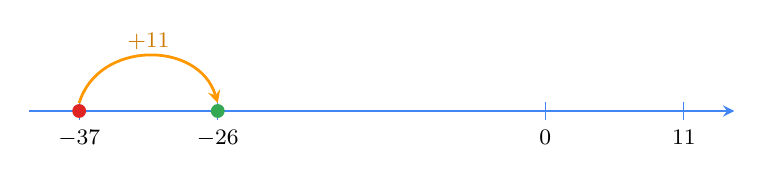
\begin{tikzpicture}[x=0.16cm,>=stealth]
\draw[->,thick,Navy] (-41,0)--(15,0);
\foreach \i in {-37,-26,0,11}{\draw[Navy] (\i,0.12)--(\i,-0.12); \node[below,font=\footnotesize] at (\i,-0.12){$\i$};}
\fill[AnsRed] (-37,0) circle (2.5pt); \fill[tmGreen] (-26,0) circle (2.5pt);
\draw[->,tmOrange,line width=1pt] (-37,0.1) .. controls (-35.5,0.9) and (-27.5,0.9) .. (-26,0.1);
\node[above,font=\footnotesize,text=tmOrange!80!black,inner sep=2pt] at (-31.5,0.7){$+11$};
\end{tikzpicture}\end{center}
Trên trục số: từ $-37$ đi sang phải $11$ bước thì đến $-26$.
\begin{warnbox}Quên đổi dấu khi chuyển vế, viết $x=-26+11=-15$, là sai (phương án C). Thử lại: $-15+11=-4\neq -26$.\end{warnbox}
\begin{parentbox}Có thể giải thích bằng chuyện nợ tiền: ``Sau khi được cho $\$11$ để trả bớt nợ, bạn vẫn còn nợ $\$26$. Lúc đầu bạn nợ bao nhiêu?'' Lúc đầu nợ nhiều hơn: $26+11=37$ đô la, tức là $-37$.\end{parentbox}
\verify{$(-37)+11=-26$. Đúng.}
Vậy chọn \textbf{(A)}.
\ans{(A) $-37$}
}

% ---------------------------------------------------------------- Bài 10
\begin{probbox}{10}{\relax}
Ông Mikhail có $\$10\,000$, toàn bộ là tờ $\$50$. Hỏi ông có bao nhiêu tờ $\$50$?
\choices{$1\,000$}{$200$}{$1\,250$}{$500$}{$2\,000$}
\end{probbox}
\probsol{
\textbf{Phân tích đề.} Tổng số tiền là $\$10\,000$ (mười nghìn đô la). Mỗi tờ có mệnh giá $\$50$. Cần tìm số tờ.
\begin{recallbox}Số tờ tiền $=$ tổng số tiền $:$ mệnh giá một tờ.\end{recallbox}
\step{1}{Gọi ẩn và lập phương trình}
Gọi $n$ là số tờ $\$50$ ($n$ là số tự nhiên). Giá trị của $n$ tờ là $50n$ đô la, nên $50n=10\,000$.
\step{2}{Giải: chia cả hai vế cho $50$, tính gọn bằng cách bỏ bớt chữ số $0$}
$n=10\,000:50$. Bỏ một chữ số $0$ ở cả số bị chia và số chia (tức là chia cả hai cho $10$, thương không đổi): $10\,000:50=1\,000:5=200$.
\step{3}{Một cách nghĩ khác}
$2$ tờ $\$50$ là $\$100$. Mười nghìn đô la gồm $100$ lần $\$100$, nên có $100\times 2=200$ tờ.
\verify{$200\times 50=10\,000$ đô la. Đúng.}
\begin{warnbox}Đếm sai số chữ số $0$ là lỗi rất hay gặp: $10\,000:50$ \emph{không} phải $2\,000$ (phương án E) hay $1\,000$ (phương án A). Nên viết số có dấu cách giữa các nhóm ba chữ số ($10\,000$) để đếm cho chính xác.\end{warnbox}
Vậy chọn \textbf{(B)}.
\begin{parentbox}Có thể dùng tiền đồ chơi: một xấp $10$ tờ $\$50$ là $\$500$. Hỏi con: cần bao nhiêu xấp như vậy để có $\$10\,000$? ($20$ xấp, tức $200$ tờ.)\end{parentbox}
\ans{(B) $200$}
}

% ---------------------------------------------------------------- Bài 11

\begin{probbox}{11}{\relax}
Tích $60\times 60\times 24\times 7$ bằng
\choicesL{số phút trong bảy tuần}{số giờ trong sáu mươi ngày}{số giây trong bảy giờ}{số giây trong một tuần}{số phút trong hai mươi bốn tuần}
\end{probbox}
\probsol{
\textbf{Phân tích đề.} Không cần tính tích ra số. Hãy đọc mỗi thừa số như một bước đổi đơn vị thời gian.
\begin{recallbox}$1$ tuần $=7$ ngày;\ \ $1$ ngày $=24$ giờ;\ \ $1$ giờ $=60$ phút;\ \ $1$ phút $=60$ giây.\end{recallbox}
\step{1}{Đọc tích từ phải sang trái}
\begin{itemize}[leftmargin=1.4em,itemsep=1pt,topsep=1pt]
\item $7$ là số ngày trong \textbf{một tuần};
\item $24\times 7$ là số giờ trong một tuần;
\item $60\times 24\times 7$ là số phút trong một tuần;
\item $60\times 60\times 24\times 7$ là số \textbf{giây} trong một tuần.
\end{itemize}
\step{2}{Kiểm tra các phương án còn lại bằng cách viết tích của chúng}
\begin{center}
\begin{tabular}{|c|l|r|}
\hline
\rowcolor{tmBlue!10} Phương án & Biểu thức & Giá trị\\ \hline
(A) phút trong $7$ tuần & $60\times 24\times 7\times 7$ & $70\,560$\\ \hline
(B) giờ trong $60$ ngày & $24\times 60$ & $1\,440$\\ \hline
(C) giây trong $7$ giờ & $60\times 60\times 7$ & $25\,200$\\ \hline
(D) giây trong $1$ tuần & $60\times 60\times 24\times 7$ & $604\,800$\\ \hline
(E) phút trong $24$ tuần & $60\times 24\times 7\times 24$ & $241\,920$\\ \hline
\end{tabular}
\end{center}
Chỉ phương án (D) có đúng tích $60\times 60\times 24\times 7=604\,800$.
\begin{warnbox}Thấy các số $60$, $24$, $7$ xuất hiện trong câu chữ, nhiều bạn chọn vội (A) hoặc (E). Phải ghép đúng \emph{từng} bước đổi đơn vị: (A) thiếu một thừa số $60$ và thừa một thừa số $7$.\end{warnbox}
Vậy chọn \textbf{(D)}.
\ans{(D) số giây trong một tuần}
}

% ---------------------------------------------------------------- Bài 12
\begin{probbox}{12}{\stars{1}}
Bốn số $a$, $b$, $c$, $d$ đều là số nguyên dương lớn hơn $3$ và thoả mãn
\[\frac{1}{a-2}=\frac{1}{b+2}=\frac{1}{c+1}=\frac{1}{d-3}.\]
Cách sắp xếp nào dưới đây là đúng?
\choicesII{$a<b<c<d$}{$c<b<a<d$}{$b<a<c<d$}{$d<a<c<b$}{$b<c<a<d$}
\end{probbox}
\probsol{
\textbf{Phân tích đề.} Bốn phân số có cùng tử số $1$ và bằng nhau. Cần so sánh $a,b,c,d$.
(Điều kiện ``lớn hơn $3$'' bảo đảm các mẫu số đều khác $0$, các phân số có nghĩa.)
\step{1}{Phân số cùng tử bằng nhau thì mẫu bằng nhau}
\begin{recallbox}Nếu $\dfrac{1}{p}=\dfrac{1}{q}$ thì $p=q$ (nhân chéo: $1\cdot q=1\cdot p$).\end{recallbox}
Do đó: $a-2=b+2=c+1=d-3$.
\step{2}{Đặt giá trị chung là $k$ rồi biểu diễn từng số theo $k$}
$a-2=k\Rightarrow a=k+2$;\quad $b+2=k\Rightarrow b=k-2$;\quad $c+1=k\Rightarrow c=k-1$;\quad $d-3=k\Rightarrow d=k+3$.
\step{3}{So sánh với cùng mốc $k$}
Các ``phần thêm'' là $-2$ (của $b$), $-1$ (của $c$), $+2$ (của $a$), $+3$ (của $d$). Vì $-2<-1<2<3$ nên
\[k-2<k-1<k+2<k+3,\quad\text{tức là}\quad b<c<a<d.\]
\begin{center}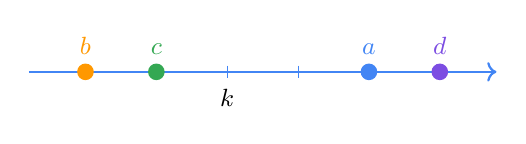
\begin{tikzpicture}[x=0.9cm]
\draw[->,thick,Navy] (-2.8,0)--(3.8,0);
\foreach \i in {-2,...,3}{\draw[Navy] (\i,0.08)--(\i,-0.08);}
\node[below,font=\small] at (0,-0.1){$k$};
\foreach \i/\l/\c in {-2/b/tmOrange,-1/c/tmGreen,2/a/tmBlue,3/d/tmPurple}{\fill[\c] (\i,0) circle (3pt); \node[above,font=\small\bfseries,text=\c] at (\i,0.1){$\l$};}
\end{tikzpicture}\end{center}
\begin{warnbox}Nhìn ``$a-2$'' có dấu trừ, nhiều bạn nghĩ $a$ nhỏ. Nhưng $a$ phải \emph{bớt đi} $2$ mới bằng $k$, nên $a$ lớn hơn $k$. Ngược lại $b$ phải \emph{thêm} $2$ mới bằng $k$, nên $b$ nhỏ hơn $k$.\end{warnbox}
\verify{Chọn thử $k=6$ (để cả bốn số đều lớn hơn $3$): $a=8$, $b=4$, $c=5$, $d=9$ (đều lớn hơn $3$). Khi đó $\dfrac{1}{8-2}=\dfrac{1}{4+2}=\dfrac{1}{5+1}=\dfrac{1}{9-3}=\dfrac{1}{6}$ và quả thật $4<5<8<9$, tức $b<c<a<d$.}
Thứ tự $b<c<a<d$ là phương án \textbf{(E)}.
\ans{(E) $b<c<a<d$}
}

% ---------------------------------------------------------------- Bài 13
\begin{probbox}{13}{\relax}
Một hình chữ nhật có chiều dài $x$ và chiều rộng $y$. Một tam giác có cạnh đáy bằng $16$ và chiều cao tương ứng bằng $x$.
Nếu diện tích hình chữ nhật bằng diện tích tam giác thì giá trị của $y$ là
\choices{$16$}{$4$}{$8$}{$12$}{$32$}
\end{probbox}
\probsol{
\textbf{Phân tích đề.} Hình chữ nhật: dài $x$, rộng $y$. Tam giác: đáy $16$, cao $x$. Hai diện tích bằng nhau. Tìm $y$
(lưu ý: đề không cho $x$, nhưng ta sẽ thấy $x$ tự ``biến mất'').
\begin{figC}
\draw[tmBlue,line width=1pt,fill=tmBlue!10] (0,0) rectangle (2.4,2.0); % y=8 -> 2,0 (cùng tỉ lệ với đáy 16 -> 4)
\node[below] at (1.2,0){$x$}; \node[left] at (0,1.0){$y$};
\draw[tmOrange!85!black,line width=1pt,fill=tmOrange!12] (3.6,0)--(7.6,0)--(4.6,2.4)--cycle;
\draw[dashed,Slate] (4.6,2.4)--(4.6,0); \draw[Slate] (4.6,0.18)--(4.78,0.18)--(4.78,0);
\node[below] at (5.6,0){$16$}; \node[left,font=\small] at (4.6,1.1){$x$};
\end{figC}
\step{1}{Viết hai công thức diện tích}
\begin{recallbox}Diện tích hình chữ nhật $=$ dài $\times$ rộng. Diện tích tam giác $=\dfrac{\text{đáy}\times\text{chiều cao}}{2}$.\end{recallbox}
Hình chữ nhật: $S_1=x\cdot y=xy$.\quad Tam giác: $S_2=\dfrac{16\cdot x}{2}=8x$.
\step{2}{Lập phương trình và giải}
$xy=8x$. Vì $x$ là một độ dài nên $x>0$; chia cả hai vế cho $x$: $y=8$.
\begin{proofbox}Có thể hiểu không cần chia: $x\cdot y$ và $x\cdot 8$ là ``$x$ nhóm $y$'' và ``$x$ nhóm $8$''. Hai tích bằng nhau với cùng số nhóm $x\neq 0$ thì mỗi nhóm phải bằng nhau: $y=8$.\end{proofbox}
\begin{warnbox}Quên chia đôi khi tính diện tích tam giác sẽ dẫn đến $y=16$ (phương án A).\end{warnbox}
\verify{Thử $x=5$: hình chữ nhật $5\times 8=40$; tam giác $\dfrac{16\cdot 5}{2}=40$. Bằng nhau. (Với $x$ bất kì cũng đúng.)}
Vậy chọn \textbf{(C)}.
\ans{(C) $8$}
}

% ---------------------------------------------------------------- Bài 14
\begin{probbox}{14}{\relax}
Kí hiệu \aeaBox{3}{4}{5}{6} được tính theo quy tắc: $3\times 6+4\times 5=38$. Biết rằng \aeaBox{2}{6}{1}{\ } có giá trị bằng $16$.
Số cần điền vào ô trống là
\choices{$1$}{$2$}{$3$}{$4$}{$5$}
\end{probbox}
\probsol{
\textbf{Phân tích đề.} Trước hết phải hiểu quy tắc từ ví dụ đã cho, rồi áp dụng cho ô có số chưa biết.
\step{1}{Tìm quy tắc}
Trong \aeaBox{3}{4}{5}{6}: $3$ (trên trái) nhân $6$ (dưới phải), cộng với $4$ (trên phải) nhân $5$ (dưới trái): $3\times 6+4\times 5=18+20=38$.
Tức là: \emph{nhân hai số theo mỗi đường chéo rồi cộng lại}. Tổng quát, \aeaBox{a}{b}{c}{d} $=a\times d+b\times c$.
\step{2}{Đặt ẩn cho ô trống và lập phương trình}
Gọi số ở ô trống (dưới phải) là $x$. Theo quy tắc: \aeaBox{2}{6}{1}{x} $=2\times x+6\times 1=2x+6$.
Đề cho giá trị bằng $16$: $2x+6=16$.
\step{3}{Giải}
Trừ $6$ ở hai vế: $2x=10$. Chia hai vế cho $2$: $x=5$.
\verify{$2\times 5+6\times 1=10+6=16$. Đúng.}
\begin{warnbox}Đừng ghép nhầm cặp: $2\times 6+1\times x$ (nhân theo hàng) là sai quy tắc; với cách đó sẽ ra $x=4$ (phương án D). Hãy kiểm tra quy tắc với ví dụ $38$ trước khi dùng.\end{warnbox}
Vậy chọn \textbf{(E)}.
\begin{parentbox}Hãy cùng con ``sáng chế'' một kí hiệu mới (chẳng hạn nhân theo hàng rồi trừ) và đố nhau. Điều quan trọng là luôn kiểm tra quy tắc với ví dụ mẫu trước khi dùng.\end{parentbox}
\ans{(E) $5$}
}

% ---------------------------------------------------------------- Bài 15
\begin{probbox}{15}{\relax}
Người ta cân ba quả bí ngô theo từng cặp, đủ mọi cách ghép đôi. Khối lượng của các cặp lần lượt là $12$ kg, $13$ kg và $15$ kg.
Quả bí nhẹ nhất nặng bao nhiêu?
\choices{$4$ kg}{$5$ kg}{$6$ kg}{$7$ kg}{$8$ kg}
\end{probbox}
\probsol{
\textbf{Phân tích đề.} Ba quả bí ghép đôi thì có đúng $3$ cặp. Gọi khối lượng ba quả từ nhẹ đến nặng là $a\le b\le c$ (kg).
Cặp nhẹ nhất là hai quả nhẹ nhất, cặp nặng nhất là hai quả nặng nhất:
$a+b=12$, \ $a+c=13$, \ $b+c=15$.
\step{1}{Cộng cả ba cặp}
Mỗi quả có mặt trong đúng \emph{hai} cặp: $(a+b)+(a+c)+(b+c)=12+13+15=40$, tức $2(a+b+c)=40$.
\begin{recallbox}Ba vật cân từng đôi: tổng ba vật bằng một nửa tổng các kết quả cân.\end{recallbox}
\step{2}{Tổng khối lượng ba quả}
$a+b+c=40:2=20$ (kg).
\step{3}{Tìm quả nhẹ nhất}
Quả nhẹ nhất $a$ là quả \emph{không} có mặt trong cặp nặng nhất ($b+c=15$):
$a=(a+b+c)-(b+c)=20-15=5$ (kg).
(Tương tự: $b=20-13=7$ kg, \ $c=20-12=8$ kg.)
\begin{tipbox}\textbf{Cách khác (thế).} Từ $a+b=12$ có $b=12-a$; từ $a+c=13$ có $c=13-a$. Thay vào $b+c=15$:
$(12-a)+(13-a)=15$, tức $25-2a=15$, nên $2a=10$ và $a=5$.\end{tipbox}
\verify{$5+7=12$, \ $5+8=13$, \ $7+8=15$. Đúng cả ba cặp.}
\begin{warnbox}Đừng lấy $12:2=6$ kg và cho rằng mỗi quả trong cặp nhẹ nhất nặng $6$ kg: hai quả trong một cặp không nhất thiết nặng bằng nhau. Phương án (E) $8$ kg là quả \emph{nặng nhất}.\end{warnbox}
Quả nhẹ nhất nặng $5$ kg, ứng với phương án \textbf{(B)}.
\begin{parentbox}Cho con dùng ba đồ vật trong nhà và một chiếc cân: cân từng cặp, cộng ba kết quả rồi chia đôi, so với khi đặt cả ba lên cân. Con sẽ tự thấy vì sao phải chia $2$.\end{parentbox}
\ans{(B) $5$ kg}
}

% ---------------- part b ----------------
% ===== Topic 1, part b (VI): problems 16-30 =====
% helper shapes for the balance-scale problems (topic-specific prefix \ae...)
% \aeShp{code}{x}{y}: draw shape (T triangle, C circle, S square, D diamond, Q question mark) with lower-left corner at (x,y)
\providecommand{\aeShp}[3]{%
  \if#1T\draw[tmBlue!80!black,line width=0.8pt,fill=tmBlue!18] (#2,#3)--(#2+0.34,#3)--(#2+0.17,#3+0.3)--cycle;\fi
  \if#1C\draw[tmOrange!85!black,line width=0.8pt,fill=tmOrange!22] (#2+0.15,#3+0.15) circle (0.15);\fi
  \if#1S\draw[tmGreen!80!black,line width=0.8pt,fill=tmGreen!18] (#2,#3) rectangle (#2+0.3,#3+0.3);\fi
  \if#1D\draw[tmPurple!85!black,line width=0.8pt,fill=tmPurple!18] (#2+0.13,#3)--(#2+0.26,#3+0.16)--(#2+0.13,#3+0.32)--(#2,#3+0.16)--cycle;\fi
  \if#1Q\node[font=\Large\bfseries,text=Ink,inner sep=0pt,anchor=south] at (#2+0.15,#3) {?};\fi}
\providecommand{\aeTri}{\tikz[baseline=0pt]{\aeShp{T}{0}{0}}}
\providecommand{\aeCir}{\tikz[baseline=0pt]{\aeShp{C}{0}{0}}}
\providecommand{\aeSq}{\tikz[baseline=0pt]{\aeShp{S}{0}{0}}}
\providecommand{\aeDia}{\tikz[baseline=0pt]{\aeShp{D}{0}{0}}}
% \aeRow{list}{xcentre}{y}: a row of shapes (e.g. {T,C}) centred at xcentre, standing on height y
\providecommand{\aeRow}[3]{%
  \foreach \aeS [count=\aeI] in {#1}{\xdef\aeN{\aeI}}%
  \foreach \aeS [count=\aeI] in {#1}{\aeShp{\aeS}{#2-0.19*\aeN+0.38*\aeI-0.36}{#3+0.03}}}
% \aeScale{x}{y}{left list}{right list}: a balanced scale centred at (x,y)
\providecommand{\aeScale}[4]{\begin{scope}[shift={(#1,#2)}]
  \draw[Ink,line width=1pt] (-1.9,0.55)--(-0.5,0.55) (-1.2,0.55)--(-1.2,0.25)--(1.2,0.25)--(1.2,0.55) (0.5,0.55)--(1.9,0.55);
  \draw[Ink,line width=0.9pt,fill=Ink!12] (-0.2,-0.12)--(0,0.25)--(0.2,-0.12)--cycle;
  \aeRow{#3}{-1.2}{0.55}\aeRow{#4}{1.2}{0.55}
\end{scope}}

% ------------------------------------------------------------------ 16
\begin{probbox}{16}{\relax}
Bạn Rosie đang tập tiết kiệm. Hôm nay trong tài khoản của Rosie có $\$120$. Từ nay, mỗi lần gửi tiết kiệm Rosie sẽ gửi thêm đúng $\$30$. Nếu Rosie gửi $m$ lần như vậy thì biểu thức nào dưới đây biểu thị đúng số tiền (tính bằng đô la) có trong tài khoản?
\choices{$120+m$}{$30m$}{$30+120m$}{$150m$}{$120+30m$}
\end{probbox}
\probsol{
\textbf{Phân tích đề.} Cho biết: lúc đầu có $\$120$; mỗi lần gửi thêm $\$30$; gửi $m$ lần. Cần tìm: biểu thức đại số cho tổng số tiền sau $m$ lần gửi.

\step{1}{Thử với vài giá trị cụ thể của $m$ để thấy quy luật}
\begin{center}
\begin{tabular}{|c|c|c|}
\hline
\rowcolor{tmBlue!10}\textbf{Số lần gửi} & \textbf{Số tiền gửi thêm} & \textbf{Tổng số tiền (đô la)}\\ \hline
$0$ & $0$ & $120$\\ \hline
$1$ & $30$ & $120+30=150$\\ \hline
$2$ & $30+30=30\cdot 2=60$ & $120+60=180$\\ \hline
$3$ & $30\cdot 3=90$ & $120+90=210$\\ \hline
$m$ & $30\cdot m=30m$ & $120+30m$\\ \hline
\end{tabular}
\end{center}

\step{2}{Viết biểu thức}
Số tiền \emph{gửi thêm} sau $m$ lần là $m$ lần của $30$, tức là $30m$. Cộng với số tiền có sẵn $120$, ta được
\[ \text{Tổng số tiền} = 120 + 30m \ \text{(đô la)}. \]
\begin{recallbox}$30m$ nghĩa là $30\cdot m$ (ta được phép bỏ dấu nhân giữa một số và một chữ). Cộng một số $a$ lặp lại $m$ lần thì được $a\cdot m$.\end{recallbox}

\step{3}{Loại các phương án sai}
\begin{itemize}[leftmargin=1.3em,itemsep=1pt]
\item (A) $120+m$: chỉ cộng thêm $\$1$ mỗi lần -- sai.
\item (B) $30m$: quên mất $\$120$ có sẵn. Với $m=0$ cho $0$ -- sai.
\item (C) $30+120m$: đảo vai trò hai số. Với $m=1$ cho $150$ (trùng!) nhưng với $m=2$ cho $270\ne 180$ -- sai.
\item (D) $150m$: với $m=2$ cho $300\ne 180$ -- sai.
\end{itemize}
\begin{warnbox}Thử với \emph{một} giá trị $m=1$ là chưa đủ: cả (C), (D) và (E) đều cho $150$. Hãy thử thêm $m=0$ hoặc $m=2$ để phân biệt.\end{warnbox}
\verify{Với $m=3$: $120+30\cdot 3=210$, đúng như bảng ở Bước 1.}
Vậy chọn \textbf{(E)}.
\ans{(E) $120+30m$}
}

% ------------------------------------------------------------------ 17
\begin{probbox}{17}{\relax}
Cả bốn chiếc cân dưới đây đều đang thăng bằng. Các hình giống nhau có khối lượng bằng nhau. Một cách có thể thay vào dấu ``?'' để chiếc cân thứ tư thăng bằng là
\begin{figC}
\aeScale{0}{1.6}{T,C}{S}
\aeScale{4.6}{1.6}{T}{D,C}
\aeScale{0}{0}{D,T}{C,S}
\aeScale{4.6}{0}{C,D,T}{Q}
\node[font=\footnotesize\bfseries,text=Slate] at (-2.25,2.45) {1};
\node[font=\footnotesize\bfseries,text=Slate] at (2.35,2.45) {2};
\node[font=\footnotesize\bfseries,text=Slate] at (-2.25,0.85) {3};
\node[font=\footnotesize\bfseries,text=Slate] at (2.35,0.85) {4};
\end{figC}
\choices{\aeTri\,\aeSq}{\aeDia\,\aeTri}{\aeCir\,\aeSq}{\aeSq\,\aeDia}{\aeTri\,\aeCir}
\end{probbox}
\probsol{
\textbf{Phân tích đề.} Mỗi chiếc cân thăng bằng cho ta một \emph{đẳng thức}: tổng khối lượng đĩa trái bằng tổng khối lượng đĩa phải. Ta viết thẳng các hình vào đẳng thức (mỗi hình thay cho khối lượng của nó):
\[
\text{Cân 1: } \aeTri+\aeCir=\aeSq,\qquad
\text{Cân 2: } \aeTri=\aeDia+\aeCir,\qquad
\text{Cân 3: } \aeDia+\aeTri=\aeCir+\aeSq.
\]
Cần tìm: đĩa phải của cân 4 phải nặng bằng $\aeCir+\aeDia+\aeTri$. Ý tưởng: đổi mọi hình về cùng một ``đơn vị'' là \aeCir.
\begin{recallbox}Nếu cân thăng bằng thì khi \emph{thay} một vật bằng các vật nặng bằng nó, hoặc \emph{bỏ bớt} những vật giống nhau ở cả hai đĩa, cân vẫn thăng bằng. Đây chính là tính chất của đẳng thức: $a=b \Rightarrow a+c=b+c$ và $a-c=b-c$.\end{recallbox}

\step{1}{Dùng cân 2 để thay \aeTri\ trong cân 1}
Theo cân 2, $\aeTri=\aeDia+\aeCir$. Thay vào cân 1:
\[ \aeSq=\aeTri+\aeCir=(\aeDia+\aeCir)+\aeCir=\aeDia+2\,\aeCir. \]

\step{2}{Thay vào cân 3 để tìm \aeDia}
Đĩa trái cân 3: $\aeDia+\aeTri=\aeDia+(\aeDia+\aeCir)=2\,\aeDia+\aeCir$.\par
Đĩa phải cân 3: $\aeCir+\aeSq=\aeCir+(\aeDia+2\,\aeCir)=\aeDia+3\,\aeCir$.\par
Vậy $2\,\aeDia+\aeCir=\aeDia+3\,\aeCir$. Bỏ bớt một \aeDia\ và một \aeCir\ ở cả hai đĩa:
\[ \aeDia = 2\,\aeCir. \]

\step{3}{Đổi mọi hình về đơn vị \aeCir}
\[ \aeDia=2\,\aeCir,\qquad \aeTri=\aeDia+\aeCir=3\,\aeCir,\qquad \aeSq=\aeDia+2\,\aeCir=4\,\aeCir. \]
Đĩa trái cân 4: $\aeCir+\aeDia+\aeTri=1+2+3=6$ (\aeCir).

\step{4}{Tính từng phương án (theo đơn vị \aeCir)}
\begin{center}
\begin{tabular}{|c|c|c|c|c|c|}
\hline
\rowcolor{tmBlue!10} & (A) \aeTri\,\aeSq & (B) \aeDia\,\aeTri & (C) \aeCir\,\aeSq & (D) \aeSq\,\aeDia & (E) \aeTri\,\aeCir\\ \hline
Khối lượng & $3+4=7$ & $2+3=5$ & $1+4=5$ & $4+2=\mathbf{6}$ & $3+1=4$\\ \hline
\end{tabular}
\end{center}
Chỉ có (D) nặng đúng $6$ \aeCir.
\verify{Lấy \aeCir\ nặng $1$~kg thì \aeDia, \aeTri, \aeSq\ nặng $2$, $3$, $4$~kg. Cân 1: $3+1=4$ \checkmark; cân 2: $3=2+1$ \checkmark; cân 3: $2+3=1+4$ \checkmark; cân 4: $1+2+3=6=4+2$ \checkmark.}
\begin{tipbox}Khi có nhiều ẩn, hãy chọn \emph{một} hình làm đơn vị đo và biểu diễn mọi hình khác theo nó -- giống như đổi mọi số tiền ra cùng một loại tờ tiền.\end{tipbox}
Vậy chọn \textbf{(D)}.
\ans{(D) \aeSq\,\aeDia}
}

% ------------------------------------------------------------------ 18
\begin{probbox}{18}{\relax}
Số cần điền vào ô trống để có đẳng thức đúng $\dfrac{3}{7}=\dfrac{\square}{63}$ là
\choices{$27$}{$9$}{$59$}{$63$}{$3$}
\end{probbox}
\probsol{
\textbf{Phân tích đề.} Hai phân số bằng nhau, đã biết mẫu của phân số thứ hai là $63$. Cần tìm tử số.
\begin{recallbox}\textbf{Tính chất cơ bản của phân số:} nếu nhân cả tử và mẫu của một phân số với cùng một số khác $0$ thì được một phân số bằng nó: $\dfrac{a}{b}=\dfrac{a\cdot k}{b\cdot k}$ $(k\ne 0)$.\end{recallbox}

\step{1}{Mẫu số đã được nhân với bao nhiêu?}
Từ $7$ lên $63$: $63:7=9$. Vậy mẫu số đã được nhân với $9$.

\step{2}{Nhân tử số với cùng số đó}
Để phân số không đổi, tử số cũng phải nhân với $9$: $3\cdot 9=27$.
\[ \frac{3}{7}=\frac{3\cdot 9}{7\cdot 9}=\frac{27}{63}. \]

\step{3}{Cách khác: dùng ``tích chéo''}
Hai phân số $\frac{a}{b}=\frac{c}{d}$ khi và chỉ khi $a\cdot d=b\cdot c$. Gọi số cần điền là $x$: $3\cdot 63=7\cdot x$, tức $189=7x$, nên $x=189:7=27$.
\begin{warnbox}Một số bạn thấy $63-7=56$ rồi lấy $3+56=59$ (phương án C). Phân số không thay đổi khi \emph{cộng} cùng một số vào tử và mẫu! Phải \emph{nhân} (hoặc chia).\end{warnbox}
\verify{$27:63$ rút gọn cho $9$ được $3:7$, tức $\dfrac{27}{63}=\dfrac{3}{7}$ \checkmark.}
Vậy chọn \textbf{(A)}.
\ans{(A) $27$}
}

% ------------------------------------------------------------------ 19
\begin{probbox}{19}{\relax}
Tổng của bốn số bằng $T$. Mỗi số trong bốn số đó được tăng thêm $1$ đơn vị. Cộng bốn số mới lại, rồi nhân tổng vừa được với $3$. Kết quả cuối cùng bằng
\choices{$3T+3$}{$3T+4$}{$3T+12$}{$T+12$}{$12T$}
\end{probbox}
\probsol{
\textbf{Phân tích đề.} Bốn số chưa biết, chỉ biết tổng của chúng là $T$. Ta không cần biết từng số -- chỉ cần theo dõi \emph{tổng} thay đổi thế nào.

\step{1}{Đặt tên các số}
Gọi bốn số là $a$, $b$, $c$, $d$. Theo đề: $a+b+c+d=T$.

\step{2}{Tăng mỗi số thêm 1 rồi cộng lại}
Bốn số mới là $a+1$, $b+1$, $c+1$, $d+1$. Tổng của chúng:
\[ (a+1)+(b+1)+(c+1)+(d+1)=(a+b+c+d)+(1+1+1+1)=T+4. \]
\begin{recallbox}Phép cộng có tính chất giao hoán và kết hợp, nên ta được phép nhóm các chữ với nhau và các số với nhau.\end{recallbox}

\step{3}{Nhân với 3}
\[ 3\cdot(T+4)=3\cdot T+3\cdot 4=3T+12. \]
\begin{recallbox}\textbf{Tính chất phân phối:} $k\cdot(x+y)=k\cdot x+k\cdot y$. Phải nhân $3$ với \emph{từng} số hạng trong ngoặc.\end{recallbox}
\begin{warnbox}Hai lỗi hay gặp: (1) chỉ cộng $1$ vào tổng (thay vì $4$, vì có bốn số) rồi được $3T+3$; (2) quên nhân $3$ với số $4$ rồi được $3T+4$.\end{warnbox}
\verify{Lấy bốn số $1,2,3,4$: $T=10$. Số mới $2,3,4,5$ có tổng $14$; nhân $3$ được $42$. Còn $3T+12=30+12=42$ \checkmark. Các phương án khác cho $33$, $34$, $22$, $120$ -- đều sai.}
Vậy chọn \textbf{(C)}.
\ans{(C) $3T+12$}
}

% ------------------------------------------------------------------ 20
\begin{probbox}{20}{\relax}
Hai tam giác cân, mỗi tam giác đều có ít nhất một góc bằng $70^\circ$. Ở tam giác thứ nhất, số đo (theo độ) của mỗi góc trong hai góc còn lại là số chẵn. Ở tam giác thứ hai, số đo của mỗi góc trong hai góc còn lại là số lẻ. Gọi $S$ là tổng hai góc bằng nhau của tam giác thứ nhất và $T$ là tổng hai góc bằng nhau của tam giác thứ hai. Giá trị của $S+T$ là
\choices{$280^\circ$}{$250^\circ$}{$220^\circ$}{$200^\circ$}{$300^\circ$}
\end{probbox}
\probsol{
\textbf{Phân tích đề.} Một tam giác cân có hai góc ở đáy bằng nhau. Góc $70^\circ$ có thể là \emph{góc ở đỉnh} hoặc \emph{góc ở đáy}. Ta xét cả hai khả năng, rồi xem khả năng nào cho ``hai góc còn lại chẵn'', khả năng nào cho ``hai góc còn lại lẻ''.
\begin{recallbox}Tổng ba góc trong một tam giác bằng $180^\circ$. Trong tam giác cân, hai góc ở đáy bằng nhau.\end{recallbox}

\step{1}{Khả năng 1: góc $70^\circ$ là góc ở đáy}
Khi đó góc ở đáy còn lại cũng bằng $70^\circ$. Góc ở đỉnh bằng $180^\circ-70^\circ-70^\circ=40^\circ$.\par
Ba góc: $70^\circ,\ 70^\circ,\ 40^\circ$. Hai góc còn lại (ngoài một góc $70^\circ$) là $70^\circ$ và $40^\circ$ -- \textbf{đều chẵn}.

\step{2}{Khả năng 2: góc $70^\circ$ là góc ở đỉnh}
Hai góc ở đáy bằng nhau và có tổng $180^\circ-70^\circ=110^\circ$, nên mỗi góc bằng $110^\circ:2=55^\circ$.\par
Ba góc: $70^\circ,\ 55^\circ,\ 55^\circ$. Hai góc còn lại là $55^\circ$ và $55^\circ$ -- \textbf{đều lẻ}.
\begin{figC}
\begin{scope}
\draw[tmBlue,line width=1.1pt,fill=tmBlue!8] (0,0)--(1.6,0)--(0.8,2.2)--cycle;
\node[font=\scriptsize] at (0.33,0.2) {$70^\circ$};
\node[font=\scriptsize] at (1.27,0.2) {$70^\circ$};
\node[font=\scriptsize] at (0.8,1.35) {$40^\circ$};
\node[font=\footnotesize\bfseries,text=tmBlue] at (0.8,-0.35) {Tam giác thứ nhất};
\end{scope}
\begin{scope}[xshift=3.6cm]
\draw[tmOrange,line width=1.1pt,fill=tmOrange!8] (0,0)--(2.4,0)--(1.2,1.71)--cycle;
\node[font=\scriptsize] at (0.45,0.18) {$55^\circ$};
\node[font=\scriptsize] at (1.95,0.18) {$55^\circ$};
\node[font=\scriptsize] at (1.2,1.12) {$70^\circ$};
\node[font=\footnotesize\bfseries,text=tmOrange!85!black] at (1.2,-0.35) {Tam giác thứ hai};
\end{scope}
\end{figC}

\step{3}{Xác định $S$ và $T$}
Tam giác thứ nhất (hai góc còn lại chẵn) là khả năng 1. Hai góc \emph{bằng nhau} của nó là hai góc $70^\circ$: $S=70^\circ+70^\circ=140^\circ$.\par
Tam giác thứ hai (hai góc còn lại lẻ) là khả năng 2. Hai góc bằng nhau là hai góc $55^\circ$: $T=55^\circ+55^\circ=110^\circ$.

\step{4}{Tính $S+T$}
$S+T=140^\circ+110^\circ=250^\circ$.
\begin{warnbox}``Tổng hai góc bằng nhau'' là tổng hai góc \emph{ở đáy}, không phải tổng hai góc ``còn lại''. Ở tam giác thứ nhất, hai góc còn lại là $70^\circ$ và $40^\circ$ (tổng $110^\circ$), nhưng hai góc bằng nhau là $70^\circ$ và $70^\circ$ (tổng $140^\circ$). Nhầm chỗ này sẽ ra $110^\circ+110^\circ=220^\circ$ (phương án C).\end{warnbox}
\verify{$70+70+40=180$ và $70+55+55=180$ \checkmark.}
Vậy chọn \textbf{(B)}.
\ans{(B) $250^\circ$}
}

% ------------------------------------------------------------------ 21
\begin{probbox}{21}{\relax}
Bạn Andrea tham gia một chuyến chèo thuyền kayak kéo dài $6$ ngày với tổng quãng đường $168$~km. Vừa hết ngày thứ ba, Andrea đã đi được $\frac{3}{7}$ tổng quãng đường. Trong những ngày còn lại, trung bình mỗi ngày Andrea phải chèo bao nhiêu ki-lô-mét?
\choices{$29$}{$24$}{$27$}{$32$}{$26$}
\end{probbox}
\probsol{
\textbf{Phân tích đề.} Cho biết: tổng quãng đường $168$~km; chuyến đi $6$ ngày; sau $3$ ngày đã đi $\frac{3}{7}$ quãng đường. Cần tìm: số km trung bình mỗi ngày trong số ngày còn lại.
\begin{recallbox}Muốn tìm $\frac{m}{n}$ của một số, ta nhân số đó với $\frac{m}{n}$ (chia cho $n$ rồi nhân với $m$).\end{recallbox}

\step{1}{Tính quãng đường đã đi}
$\dfrac{3}{7}$ của $168$~km là $168\cdot\dfrac{3}{7}=168:7\cdot 3=24\cdot 3=72$ (km).

\step{2}{Số ngày còn lại}
Chuyến đi $6$ ngày, đã xong $3$ ngày, nên còn $6-3=3$ ngày.

\step{3}{Gọi ẩn và lập phương trình}
Gọi $x$ (km) là quãng đường trung bình Andrea phải chèo mỗi ngày trong $3$ ngày còn lại ($x>0$).
Trong $3$ ngày đó Andrea chèo được $3x$ km. Quãng đường đã đi cộng quãng đường sẽ đi bằng cả chặng:
\[ 72+3x=168. \]

\step{4}{Giải phương trình}
Chuyển vế: $3x=168-72=96$. Chia hai vế cho $3$: $x=96:3=32$ (km/ngày).
\begin{tipbox}Cũng có thể nghĩ: phần còn lại là $1-\frac{3}{7}=\frac{4}{7}$ quãng đường, tức $168:7\cdot 4=96$~km, chia đều cho $3$ ngày được $32$~km mỗi ngày.\end{tipbox}
\begin{warnbox}Đừng nhầm ``phần quãng đường còn lại'' ($\frac{4}{7}$) với ``số ngày còn lại'' ($3$ ngày). Phương án (B) $24$~km chỉ là độ dài của \emph{một phần bảy} quãng đường.\end{warnbox}
\verify{$72+3\cdot 32=72+96=168$~km \checkmark.}
Vậy chọn \textbf{(D)}.
\ans{(D) $32$~km mỗi ngày}
}

% ------------------------------------------------------------------ 22
\begin{probbox}{22}{\stars{1}}
Một chấm tròn xuất phát tại điểm $(20;19)$ trên mặt phẳng tọa độ. Ở bước thứ nhất, chấm di chuyển $1$ đơn vị theo phương ngang hoặc phương dọc, tức là đến một trong các điểm $(21;19)$, $(19;19)$, $(20;20)$ hoặc $(20;18)$. Ở bước thứ hai, chấm di chuyển $2$ đơn vị (về chiều nào cũng được) theo phương \emph{vuông góc} với bước thứ nhất. Từ đó về sau, mỗi bước dài hơn bước trước $1$ đơn vị ($3$ đơn vị, $4$ đơn vị, $5$ đơn vị, \dots) và luôn vuông góc với bước ngay trước nó. Chấm dừng lại sau $10$ bước. Điểm nào dưới đây \textbf{không thể} là vị trí cuối cùng của chấm?
\choices{$(27;33)$}{$(30;40)$}{$(21;21)$}{$(42;44)$}{$(37;37)$}
\end{probbox}
\probsol{
\textbf{Phân tích đề.} Các bước có độ dài $1,2,3,\dots,10$. ``Vuông góc với bước trước'' nghĩa là các bước \emph{luân phiên} ngang -- dọc -- ngang -- dọc\dots\ Ta cần tìm điểm mà chấm không bao giờ tới được.
\begin{recallbox}Trên mặt phẳng tọa độ, đi sang phải (trái) $k$ đơn vị làm hoành độ (số thứ nhất) tăng (giảm) $k$; đi lên (xuống) $k$ đơn vị làm tung độ (số thứ hai) tăng (giảm) $k$.\end{recallbox}

\step{1}{Tách các bước thành hai nhóm}
Nếu bước $1$ là bước ngang thì các bước ngang là bước $1,3,5,7,9$ (độ dài lẻ) và các bước dọc là bước $2,4,6,8,10$ (độ dài chẵn). Nếu bước $1$ là bước dọc thì ngược lại.\par
Mỗi bước có thể đi theo chiều dương (dấu $+$) hoặc chiều âm (dấu $-$). Vậy độ dịch chuyển theo một phương là
\[ \pm 1\pm 3\pm 5\pm 7\pm 9 \quad\text{(nhóm lẻ)},\qquad \pm 2\pm 4\pm 6\pm 8\pm 10\quad\text{(nhóm chẵn).} \]

\step{2}{Nhóm lẻ cho được những số nào?}
Nếu tất cả mang dấu $+$: $1+3+5+7+9=25$. Khi đổi dấu một bước độ dài $a$ từ $+$ sang $-$, tổng giảm đi $2a$ (mất $a$ và còn bị trừ thêm $a$). Vậy:
\[ \text{độ dịch chuyển}=25-2\times(\text{tổng các độ dài bị đổi dấu}). \]
Muốn được $21$, cần tổng các độ dài bị đổi dấu là $(25-21):2=2$. Nhưng trong $\{1,3,5,7,9\}$ không có cách chọn nào có tổng bằng $2$ (chọn $1$ thì được $1$; chọn thêm bất kỳ số nào thì đã $\ge 4$). Vậy \textbf{nhóm lẻ không thể cho độ dịch chuyển $21$} (tương tự cũng không thể cho $-21$).
\begin{proofbox}Mọi tổng con của $\{1,3,5,7,9\}$ có thể bằng: $0,1,3,4,5,6,7,8,9,\dots$ nhưng \emph{không} bằng $2$, vì số nhỏ nhất là $1$, số nhỏ thứ hai là $3$, nên chọn từ hai số trở lên thì tổng ít nhất $1+3=4$.\end{proofbox}

\step{3}{Kiểm tra phương án (B) $(30;40)$}
Độ dịch chuyển: ngang $30-20=10$, dọc $40-19=21$.\par
Một tổng có dấu của $5$ số lẻ luôn là số \emph{lẻ}; của các số chẵn luôn là số \emph{chẵn}. Vì $21$ lẻ nên phương dọc phải là nhóm lẻ, tức phải có $\pm1\pm3\pm5\pm7\pm9=21$ -- điều này không thể theo Bước 2. Vậy chấm \textbf{không thể} đến $(30;40)$.

\step{4}{Các phương án còn lại đều đến được (chỉ ra cách đi)}
\begin{center}\small
\begin{tabular}{|c|c|c|c|}
\hline
\rowcolor{tmBlue!10}\textbf{Điểm} & \textbf{Dịch chuyển (ngang; dọc)} & \textbf{Nhóm lẻ} & \textbf{Nhóm chẵn}\\ \hline
(A) $(27;33)$ & $(7;14)$ & $1+3+5+7-9=7$ & $2+4+6-8+10=14$\\ \hline
(C) $(21;21)$ & $(1;2)$ & $1-3+5+7-9=1$ & $2-4+6+8-10=2$\\ \hline
(D) $(42;44)$ & $(22;25)$ & $1+3+5+7+9=25$ & $2-4+6+8+10=22$\\ \hline
(E) $(37;37)$ & $(17;18)$ & $-1-3+5+7+9=17$ & $2+4-6+8+10=18$\\ \hline
\end{tabular}
\end{center}
(Ở (D), độ dịch chuyển ngang $22$ là số chẵn nên bước đầu tiên phải là bước dọc.) Ví dụ đường đi tới $(21;21)$: các bước lần lượt là phải $1$, lên $2$, trái $3$, xuống $4$, phải $5$, lên $6$, phải $7$, lên $8$, trái $9$, xuống $10$:
\begin{figC}\begin{scope}[scale=0.3]
\draw[Line,line width=0.3pt] (-3,-3) grid (11,13);
\draw[tmBlue,line width=1.2pt,->] (0,0)--(1,0)--(1,2)--(-2,2)--(-2,-2)--(3,-2)--(3,4)--(10,4)--(10,12)--(1,12)--(1,2);
\fill[tmGreen] (0,0) circle (9pt); \fill[AnsRed] (1,2) circle (9pt);
\end{scope}
\node[font=\scriptsize,anchor=north] at (1.2,-1.05) {\textcolor{tmGreen}{\large$\bullet$}\ điểm xuất phát $(20;19)$\qquad \textcolor{AnsRed}{\large$\bullet$}\ điểm cuối $(21;21)$};
\end{figC}
\begin{warnbox}Chỉ xét tính chẵn -- lẻ là chưa đủ: cả $10$ (chẵn) và $21$ (lẻ) đều ``hợp lệ'' về tính chẵn lẻ, nhưng $21$ vẫn không đạt được. Phải kiểm tra thật sự xem có cách chọn dấu hay không.\end{warnbox}
Vậy chọn \textbf{(B)}.
\ans{(B) $(30;40)$}
}

% ------------------------------------------------------------------ 23

\begin{probbox}{23}{\relax}
Chị Gail làm nhân viên phục vụ ở một nhà hàng. Hôm thứ Bảy, chị dậy lúc $6$\,h\,$30$ sáng, bắt đầu làm việc lúc $x$ giờ sáng và kết thúc lúc $x$ giờ chiều (cùng ngày). Hôm thứ Bảy chị Gail làm việc trong bao lâu?
\choicesII{$24-2x$ giờ}{$12-x$ giờ}{$2x$ giờ}{$0$ giờ}{$12$ giờ}
\end{probbox}
\probsol{
\textbf{Phân tích đề.} Bắt đầu lúc $x$ giờ sáng, kết thúc lúc $x$ giờ chiều. Cần tìm thời gian làm việc. Giờ dậy $6$\,h\,$30$ là thông tin \emph{thừa}, không dùng đến.
\begin{recallbox}$x$ giờ chiều (theo cách nói 12 giờ) chính là $(x+12)$ giờ theo cách tính 24 giờ. Ví dụ: $3$ giờ chiều là $15$ giờ.\end{recallbox}

\step{1}{Đổi sang cách tính 24 giờ}
Bắt đầu: $x$ giờ. Kết thúc: $x+12$ giờ.

\step{2}{Tính thời gian làm việc}
Thời gian $=$ giờ kết thúc $-$ giờ bắt đầu $=(x+12)-x=12$ (giờ).

\step{3}{Cách nghĩ khác (chia làm hai đoạn)}
\begin{figC}
\draw[Navy,line width=1pt,->] (0,0)--(8.4,0);
\foreach \x/\l in {0/{$x$ giờ sáng},4/{$12$ giờ trưa},8/{$x$ giờ chiều}}{\draw[Navy,line width=1pt] (\x,0.12)--(\x,-0.12); \node[below,font=\footnotesize] at (\x,-0.12) {\l};}
\draw[<->,tmBlue!72!black,line width=0.7pt] (0.06,0.35)--(3.94,0.35) node[midway,above,font=\footnotesize] {$12-x$ giờ};
\draw[<->,tmBlue!72!black,line width=0.7pt] (4.06,0.35)--(7.94,0.35) node[midway,above,font=\footnotesize] {$x$ giờ};
\end{figC}
Từ $x$ giờ sáng đến $12$ giờ trưa là $12-x$ giờ; từ $12$ giờ trưa đến $x$ giờ chiều là $x$ giờ. Tổng: $(12-x)+x=12$ giờ. Kết quả không phụ thuộc vào $x$!
\begin{warnbox}Phương án (B) $12-x$ chỉ là phần buổi sáng. Phương án (D) $0$ giờ xuất hiện khi lấy $x-x$ mà quên rằng một bên là ``sáng'', một bên là ``chiều''.\end{warnbox}
\verify{Nếu $x=8$: chị làm từ $8$ giờ sáng đến $8$ giờ tối ($20$ giờ), tức $20-8=12$ giờ \checkmark.}
Vậy chọn \textbf{(E)}.
\ans{(E) $12$ giờ}
}

% ------------------------------------------------------------------ 24
\begin{probbox}{24}{\stars{1}}
Một hình hộp chữ nhật kích thước $8\times 8\times n$ ($n$ là số nguyên dương) được ghép từ các hình lập phương nhỏ kích thước $1\times1\times1$. Gọi $A$ là diện tích toàn phần của hình hộp chữ nhật và $B$ là tổng diện tích toàn phần của tất cả các hình lập phương nhỏ tạo nên nó. Tổng tất cả các giá trị của $n$ để $\dfrac{B}{A}$ là một số nguyên bằng
\choices{$86$}{$90$}{$70$}{$78$}{$96$}
\end{probbox}
\probsol{
\textbf{Phân tích đề.} Cần viết $A$ và $B$ theo $n$, lập tỉ số $\frac{B}{A}$, rồi tìm mọi $n$ nguyên dương làm tỉ số này là số nguyên, cuối cùng cộng các $n$ đó lại.
\begin{figC}\begin{scope}[scale=0.8]
\draw[tmBlue,line width=1pt,fill=tmBlue!8] (0,0) rectangle (2.4,1.6);
\draw[tmBlue,line width=1pt,fill=tmBlue!8] (0,1.6)--(0.9,2.3)--(3.3,2.3)--(2.4,1.6)--cycle;
\draw[tmBlue,line width=1pt,fill=tmBlue!8] (2.4,0)--(3.3,0.7)--(3.3,2.3)--(2.4,1.6)--cycle;
\draw[tmBlue,line width=0.7pt,dashed] (0,0)--(0.9,0.7)--(3.3,0.7) (0.9,0.7)--(0.9,2.3);
\node[below,font=\footnotesize] at (1.2,0) {$8$};
\node[right,font=\footnotesize] at (3.3,1.5) {$n$};
\node[below right,font=\footnotesize] at (2.8,0.4) {$8$};
\end{scope}\end{figC}
\begin{recallbox}Hình hộp chữ nhật có ba kích thước $a,b,c$ có diện tích toàn phần (tổng diện tích $6$ mặt) là $2(ab+bc+ca)$. Hình lập phương cạnh $1$ có $6$ mặt, mỗi mặt diện tích $1$, nên diện tích toàn phần là $6$. Hình hộp $a\times b\times c$ ghép từ $a\cdot b\cdot c$ hình lập phương đơn vị.\end{recallbox}

\step{1}{Tính $A$}
$A=2(8\cdot 8+8\cdot n+8\cdot n)=2(64+16n)=128+32n$.

\step{2}{Tính $B$}
Số hình lập phương nhỏ: $8\cdot 8\cdot n=64n$. Mỗi hình có diện tích toàn phần $6$, nên $B=6\cdot 64n=384n$.

\step{3}{Rút gọn tỉ số}
\[ \frac{B}{A}=\frac{384n}{128+32n}=\frac{32\cdot 12n}{32\cdot(4+n)}=\frac{12n}{n+4}. \]

\step{4}{Tách phần nguyên}
\[ \frac{12n}{n+4}=\frac{12(n+4)-48}{n+4}=12-\frac{48}{n+4}. \]
\begin{proofbox}$12(n+4)-48=12n+48-48=12n$, nên tử số không đổi. Do đó $\frac{12n}{n+4}$ là số nguyên khi và chỉ khi $\frac{48}{n+4}$ là số nguyên, tức là $n+4$ là ước của $48$.\end{proofbox}

\step{5}{Tìm các giá trị của $n$}
Các ước dương của $48$: $1,2,3,4,6,8,12,16,24,48$. Vì $n\ge 1$ nên $n+4\ge 5$; chỉ giữ lại $6,8,12,16,24,48$:
\begin{center}
\begin{tabular}{|c|c|c|c|c|c|c|}
\hline
\rowcolor{tmBlue!10}$n+4$ & $6$ & $8$ & $12$ & $16$ & $24$ & $48$\\ \hline
$n$ & $2$ & $4$ & $8$ & $12$ & $20$ & $44$\\ \hline
$\frac{B}{A}=12-\frac{48}{n+4}$ & $4$ & $6$ & $8$ & $9$ & $10$ & $11$\\ \hline
\end{tabular}
\end{center}

\step{6}{Cộng các giá trị}
$2+4+8+12+20+44=90$.
\begin{warnbox}Đừng quên điều kiện $n\ge 1$: các ước $1,2,3,4$ của $48$ cho $n+4\le 4$, tức $n\le 0$ -- bị loại.\end{warnbox}
\verify{Với $n=2$: $A=128+64=192$, $B=768$, $\frac{B}{A}=4$ \checkmark. Với $n=44$: $A=128+1408=1536$, $B=16\,896$, $\frac{B}{A}=11$ \checkmark.}
Vậy chọn \textbf{(B)}.
\ans{(B) $90$}
}

% ------------------------------------------------------------------ 25
\begin{probbox}{25}{\stars{1}}
Ba tuyến xe buýt cắt nhau tại bến $X$ như hình vẽ (các đoạn có cùng số vạch thì dài bằng nhau). Cứ $12$ phút, xe A đi hết một lượt $P\to X\to S\to X\to P$. Cứ $20$ phút, xe B đi hết một lượt $Q\to X\to T\to X\to Q$. Cứ $28$ phút, xe C đi hết một lượt $R\to X\to U\to X\to R$. Lúc $13$\,h\,$00$, ba xe A, B, C lần lượt xuất phát từ $P$, $Q$, $R$; mỗi xe chạy với vận tốc không đổi và quay đầu ngay lập tức khi tới cuối tuyến. Các xe chạy liên tục đến $23$\,h\,$00$. Trong khoảng thời gian từ $17$\,h\,$00$ đến $22$\,h\,$00$, có bao nhiêu thời điểm mà có từ hai xe trở lên cùng có mặt tại $X$?
\begin{figC}
\draw[Ink,line width=1pt] (0,1.6)--(0,-1.6) (-2.2,0)--(2.2,0) (-1.9,-1.4)--(1.9,1.4);
\foreach \p/\q/\l/\a in {(0,1.6)/P/P/above,(0,-1.6)/S/S/below,(-2.2,0)/Q/Q/left,(2.2,0)/T/T/right,(-1.9,-1.4)/R/R/below left,(1.9,1.4)/U/U/above right}{\fill[Ink] \p circle (2pt); \node[\a,font=\small\itshape] at \p {$\l$};}
\fill[Ink] (0,0) circle (2pt); \node[below right,font=\small\itshape] at (0.05,-0.05) {$X$};
% single ticks on PX and XS
\draw[tmBlue,line width=1pt] (-0.12,0.8)--(0.12,0.8) (-0.12,-0.8)--(0.12,-0.8);
% double ticks on QX and XT
\foreach \x in {-1.1,1.1}{\draw[tmOrange,line width=1pt] (\x-0.05,-0.12)--(\x-0.05,0.12) (\x+0.05,-0.12)--(\x+0.05,0.12);}
% triple ticks on RX and XU
\foreach \t in {-0.5,0.5}{\begin{scope}[shift={(1.9*\t,1.4*\t)},rotate=36.4]
  \draw[tmGreen,line width=1pt] (-0.09,-0.12)--(-0.09,0.12) (0,-0.12)--(0,0.12) (0.09,-0.12)--(0.09,0.12);\end{scope}}
\end{figC}
\choicesII{$18$}{$19$}{$20$}{$21$}{$22$}
\end{probbox}
\probsol{
\textbf{Phân tích đề.} Mỗi xe chạy đều trên tuyến có hai nhánh dài bằng nhau. Ta tìm \emph{các thời điểm} mỗi xe có mặt tại $X$, rồi đếm các thời điểm trùng nhau. Đo thời gian $t$ bằng \emph{số phút kể từ $13$\,h\,$00$}: khi đó $17$\,h\,$00$ ứng với $t=240$ và $22$\,h\,$00$ ứng với $t=540$.

\step{1}{Xe A có mặt tại $X$ vào những lúc nào?}
Một lượt $P\to X\to S\to X\to P$ gồm $4$ đoạn dài bằng nhau ($PX=XS$), đi hết $12$ phút, nên mỗi đoạn mất $12:4=3$ phút. Xe A tới $X$ sau $3$ phút, rồi đi $X\to S\to X$ hết $6$ phút, nên tới $X$ lần nữa ở phút $9$; sau đó là phút $15, 21, 27,\dots$ Tức là
\[ t=3,\ 9,\ 15,\ 21,\dots \quad = 3\times 1,\ 3\times 3,\ 3\times 5,\ 3\times 7,\dots \]
Xe A có mặt tại $X$ đúng vào các thời điểm $t=3\times(\text{số lẻ})$.

\step{2}{Tương tự cho xe B và xe C}
Xe B: mỗi đoạn mất $20:4=5$ phút, có mặt tại $X$ khi $t=5,15,25,\dots=5\times(\text{số lẻ})$.\par
Xe C: mỗi đoạn mất $28:4=7$ phút, có mặt tại $X$ khi $t=7,21,35,\dots=7\times(\text{số lẻ})$.

\step{3}{Hai xe gặp nhau tại $X$ khi nào?}
\begin{proofbox}Xe A và B cùng ở $X$ $\iff$ $t=3\times(\text{lẻ})=5\times(\text{lẻ})$. Khi đó $t$ lẻ (tích hai số lẻ là số lẻ), và $t$ chia hết cho cả $3$ và $5$, nên chia hết cho $15$; vậy $t$ là \emph{bội lẻ của $15$}. Ngược lại, nếu $t=15\times(\text{lẻ})$ thì $t=3\times(5\times\text{lẻ})=5\times(3\times\text{lẻ})$, trong ngoặc là số lẻ, nên cả hai xe đều ở $X$.\end{proofbox}
Lập luận giống hệt: A và C cùng ở $X$ $\iff$ $t$ là bội lẻ của $21$; B và C cùng ở $X$ $\iff$ $t$ là bội lẻ của $35$; cả ba xe cùng ở $X$ $\iff$ $t$ là bội lẻ của $105$.
\begin{recallbox}Nếu một số chia hết cho hai số nguyên tố cùng nhau $a$ và $b$ thì nó chia hết cho $a\cdot b$. Ví dụ: chia hết cho $3$ và $5$ thì chia hết cho $15$.\end{recallbox}

\step{4}{Đếm trong khoảng $240\le t\le 540$}
\begin{itemize}[leftmargin=1.3em,itemsep=1pt]
\item Bội lẻ của $15$: $15\times 17=255$, \dots, $15\times 35=525$ (với $17,19,\dots,35$): \textbf{10} thời điểm.
\item Bội lẻ của $21$: $21\times 13=273$, \dots, $21\times 25=525$ (với $13,15,\dots,25$): \textbf{7} thời điểm.
\item Bội lẻ của $35$: $35\times 7=245$, \dots, $35\times 15=525$ (với $7,9,\dots,15$): \textbf{5} thời điểm.
\item Bội lẻ của $105$: $105\times 3=315$ và $105\times 5=525$: \textbf{2} thời điểm (cả ba xe).
\end{itemize}

\step{5}{Loại các thời điểm bị đếm trùng}
Hai thời điểm $t=315$ và $t=525$ có cả ba xe, nên đã được đếm \emph{ba lần} trong $10+7+5=22$ (một lần trong mỗi danh sách), trong khi chỉ được đếm một lần. Ta bớt mỗi thời điểm đi $2$ lần:
\[ 22-2\times 2=18. \]
Bảng đầy đủ $18$ thời điểm (đổi ra giờ):
\begin{center}\small
\begin{tabular}{|c|c||c|c||c|c|}
\hline
\rowcolor{tmBlue!10}Giờ & Xe & Giờ & Xe & Giờ & Xe\\ \hline
17\,h\,05 & B, C & 18\,h\,57 & A, C & 20\,h\,21 & A, C\\ \hline
17\,h\,15 & A, B & 19\,h\,15 & A, B & 20\,h\,35 & B, C\\ \hline
17\,h\,33 & A, C & 19\,h\,25 & B, C & 20\,h\,45 & A, B\\ \hline
17\,h\,45 & A, B & 19\,h\,39 & A, C & 21\,h\,03 & A, C\\ \hline
\textbf{18\,h\,15} & \textbf{A, B, C} & 19\,h\,45 & A, B & 21\,h\,15 & A, B\\ \hline
18\,h\,45 & A, B & 20\,h\,15 & A, B & \textbf{21\,h\,45} & \textbf{A, B, C}\\ \hline
\end{tabular}
\end{center}
\begin{warnbox}Xe A ở $X$ \emph{hai lần} trong mỗi lượt $12$ phút (lúc đi ra và lúc quay về), nên khoảng cách giữa hai lần là $6$ phút chứ không phải $12$ phút. Nếu chỉ dùng ``bội của $12$, $20$, $28$'' sẽ ra kết quả sai.\end{warnbox}
\verify{Đếm trực tiếp từng phút từ $240$ đến $540$ (ví dụ bằng máy tính) cũng được đúng $18$ thời điểm.}
Vậy chọn \textbf{(A)}.
\ans{(A) $18$}
}

% ------------------------------------------------------------------ 26
\begin{probbox}{26}{\relax}
Bạn Steve bắt đầu từ số $7$ và đếm tiến, mỗi lần thêm $3$, được dãy $7, 10, 13,\dots$ Bạn Dave bắt đầu từ số $2026$ và đếm lùi, mỗi lần bớt $5$, được dãy $2026, 2021, 2016,\dots$ Số nào dưới đây có mặt trong cả hai dãy?
\choices{$1009$}{$1006$}{$1003$}{$1001$}{$1011$}
\end{probbox}
\probsol{
\textbf{Phân tích đề.} Mỗi dãy gồm các số cách đều nhau. Ta tìm ``dấu hiệu nhận biết'' một số thuộc mỗi dãy, rồi kiểm tra từng phương án.

\step{1}{Dấu hiệu của dãy của Steve}
$7=2\cdot 3+1$ chia cho $3$ dư $1$. Mỗi lần cộng thêm $3$, số dư khi chia cho $3$ không đổi. Vậy mọi số trong dãy của Steve đều \textbf{chia cho $3$ dư $1$} (và $\ge 7$). Ngược lại, mọi số $\ge 7$ chia $3$ dư $1$ đều có mặt, vì nó bằng $7+3k$.

\step{2}{Dấu hiệu của dãy của Dave}
$2026=405\cdot 5+1$ chia cho $5$ dư $1$. Bớt đi $5$ không làm đổi số dư khi chia cho $5$. Vậy mọi số trong dãy của Dave đều \textbf{chia cho $5$ dư $1$} (và $\le 2026$), tức là có \textbf{chữ số tận cùng là $1$ hoặc $6$}.
\begin{recallbox}Cộng hoặc trừ một bội của $m$ không làm thay đổi số dư khi chia cho $m$. Một số chia $5$ dư $1$ khi và chỉ khi chữ số tận cùng của nó là $1$ hoặc $6$. Một số chia $3$ dư bao nhiêu thì tổng các chữ số của nó chia $3$ dư bấy nhiêu.\end{recallbox}

\step{3}{Kiểm tra từng phương án}
\begin{center}
\begin{tabular}{|c|c|c|c|}
\hline
\rowcolor{tmBlue!10}\textbf{Số} & \textbf{Tổng chữ số; dư khi chia 3} & \textbf{Chữ số tận cùng} & \textbf{Thuộc cả hai?}\\ \hline
$1009$ & $10$; dư $1$ \checkmark & $9$ $\times$ & không\\ \hline
$1006$ & $7$; dư $1$ \checkmark & $6$ \checkmark & \textbf{có}\\ \hline
$1003$ & $4$; dư $1$ \checkmark & $3$ $\times$ & không\\ \hline
$1001$ & $2$; dư $2$ $\times$ & $1$ \checkmark & không\\ \hline
$1011$ & $3$; dư $0$ $\times$ & $1$ \checkmark & không\\ \hline
\end{tabular}
\end{center}
\verify{$1006=7+3\cdot 333$ (vì $1006-7=999=3\cdot 333$), nên $1006$ là số thứ $334$ trong dãy của Steve. $2026-1006=1020=5\cdot 204$, nên $1006$ có trong dãy của Dave (sau $204$ lần bớt $5$) \checkmark.}
\begin{tipbox}Thay vì viết hàng trăm số của mỗi dãy, ta chỉ cần biết số dư -- một ``chữ ký'' chung của mọi số trong dãy.\end{tipbox}
Vậy chọn \textbf{(B)}.
\ans{(B) $1006$}
}

% ------------------------------------------------------------------ 27
\begin{probbox}{27}{\stars{1}}
Trên một đường chạy hình tròn, bạn Anna đứng ở điểm $A$, bạn Ben đứng ở điểm $B$ đối diện với $A$ (đoạn $AB$ là một đường kính). Anna chạy ngược chiều kim đồng hồ, Ben chạy cùng chiều kim đồng hồ. Hai bạn chạy với vận tốc không đổi nhưng khác nhau. Sau một thời gian, hai bạn nhận thấy các lần gặp nhau luôn diễn ra tại đúng ba vị trí cố định trên đường chạy. Tỉ số vận tốc của hai bạn là
\begin{figC}
\draw[Ink,line width=1.1pt] (0,0) circle (1.1);
\fill[Ink] (0,1.1) circle (2pt) node[above right,font=\small\itshape] {$A$};
\fill[Ink] (0,-1.1) circle (2pt) node[below right,font=\small\itshape] {$B$};
\draw[tmBlue,line width=1pt,->] (-0.2,1.33)--(-0.75,1.18);
\draw[tmOrange,line width=1pt,->] (-0.2,-1.33)--(-0.75,-1.18);
\node[font=\scriptsize,text=tmBlue] at (-1.25,1.45) {Anna};
\node[font=\scriptsize,text=tmOrange!85!black] at (-1.3,-1.45) {Ben};
\end{figC}
\choicesII{$3:2$}{$3:1$}{$4:1$}{$2:1$}{$5:2$}
\end{probbox}
\probsol{
\textbf{Phân tích đề.} Hai bạn chạy \emph{ngược chiều nhau} trên vòng tròn. Ta tìm xem giữa hai lần gặp liên tiếp, mỗi bạn chạy được bao nhiêu phần của vòng, từ đó suy ra có bao nhiêu điểm gặp nhau khác nhau.

\step{1}{Giữa hai lần gặp liên tiếp, cả hai cùng chạy được đúng 1 vòng}
\begin{proofbox}Ngay sau khi gặp nhau, hai bạn tách ra theo hai chiều ngược nhau. Khoảng cách giữa họ (đo dọc theo đường chạy) tăng dần, và họ gặp lại nhau khi tổng quãng đường hai bạn chạy được vừa đủ phủ kín cả vòng tròn. Vậy giữa hai lần gặp liên tiếp, \emph{tổng} quãng đường hai bạn chạy đúng bằng $1$ vòng. (Riêng lần gặp đầu tiên: lúc đầu hai bạn cách nhau nửa vòng nên tổng quãng đường là $\frac12$ vòng.)\end{proofbox}

\step{2}{Mỗi lần, Anna chạy được bao nhiêu phần vòng?}
Trong cùng một khoảng thời gian, quãng đường tỉ lệ với vận tốc. Nếu tỉ số vận tốc Anna : Ben là $p:q$ thì trong $1$ vòng chung, Anna chạy được $\dfrac{p}{p+q}$ vòng, Ben chạy được $\dfrac{q}{p+q}$ vòng.
\begin{recallbox}Chia một đại lượng theo tỉ số $p:q$: phần thứ nhất bằng $\frac{p}{p+q}$, phần thứ hai bằng $\frac{q}{p+q}$ của tổng.\end{recallbox}
Vậy điểm gặp sau luôn cách điểm gặp trước một cung bằng $\dfrac{p}{p+q}$ vòng (theo chiều chạy của Anna).

\step{3}{Thử với tỉ số $2:1$}
Mỗi lần Anna chạy $\frac{2}{3}$ vòng. Gọi $M_1$ là điểm gặp đầu tiên. Các điểm gặp tiếp theo cách $M_1$ lần lượt $\frac23$, $\frac43$, $\frac63=2$ vòng, \dots\ Vì đi trọn $1$ vòng thì quay về chỗ cũ, nên $\frac43$ vòng cũng là $\frac13$ vòng và $2$ vòng chính là $M_1$. Chỉ có \textbf{ba} điểm gặp: $M_1$ và hai điểm chia đường tròn thành ba phần bằng nhau. (Nếu Ben nhanh hơn, tỉ số $1:2$, kết quả tương tự.)

\step{4}{Các tỉ số khác cho bao nhiêu điểm?}
\begin{center}
\begin{tabular}{|c|c|c|c|}
\hline
\rowcolor{tmBlue!10}\textbf{Tỉ số} & \textbf{Mỗi lần Anna chạy} & \textbf{Vị trí các điểm gặp (tính từ $M_1$)} & \textbf{Số điểm}\\ \hline
(A) $3:2$ & $\frac35$ vòng & $0,\frac35,\frac15,\frac45,\frac25$ rồi lặp lại & $5$\\ \hline
(B) $3:1$ & $\frac34$ vòng & $0,\frac34,\frac24,\frac14$ rồi lặp lại & $4$\\ \hline
(C) $4:1$ & $\frac45$ vòng & $0,\frac45,\frac35,\frac25,\frac15$ & $5$\\ \hline
(D) $2:1$ & $\frac23$ vòng & $0,\frac23,\frac13$ & $\mathbf{3}$\\ \hline
(E) $5:2$ & $\frac57$ vòng & $7$ vị trí khác nhau & $7$\\ \hline
\end{tabular}
\end{center}
(Ví dụ hàng (A): $\frac35+\frac35=\frac65$, bỏ $1$ vòng còn $\frac15$; thêm $\frac35$ được $\frac45$; thêm $\frac35$ được $\frac75$, bỏ $1$ vòng còn $\frac25$; thêm $\frac35$ được $1$ vòng -- trở về $M_1$.)
\begin{figC}
\draw[Ink,line width=1.1pt] (0,0) circle (1.1);
\fill[Ink] (0,1.1) circle (2pt) node[above left=1pt,font=\small\itshape] {$A$};
\fill[Ink] (0,-1.1) circle (2pt) node[below,font=\small\itshape] {$B$};
\foreach \a in {90,210,330}{\fill[AnsRed] (\a:1.1) circle (3pt);}
\node[font=\scriptsize,text=AnsRed,anchor=east] at (210:1.25) {gặp};
\node[font=\scriptsize,text=AnsRed,anchor=west] at (330:1.25) {gặp};
\node[font=\scriptsize,text=AnsRed,anchor=south west] at (0.1,1.16) {gặp};
\end{figC}
\verify{Đường chạy dài $600$~m, Anna chạy $200$ m/phút, Ben $100$ m/phút. Lúc đầu cách nhau $300$~m, gặp lần đầu sau $300:300=1$ phút, tại điểm cách $A$ $200$~m (theo chiều của Anna). Sau đó cứ $600:300=2$ phút gặp một lần, Anna chạy thêm $400$~m mỗi lần: vị trí $200\to 600$ (tức $A$) $\to 1000$ (tức $400$~m) $\to 1400$ (tức $200$~m) \dots\ Đúng ba điểm: $0$~m, $200$~m, $400$~m, chia đường tròn làm ba phần đều -- như hình trên.}
Vậy chọn \textbf{(D)}.
\ans{(D) $2:1$}
}

% ------------------------------------------------------------------ 28
\begin{probbox}{28}{\stars{1}}
Dãy $11, 20, 31, 51, 82$ là một ví dụ về một dãy tăng gồm năm số nguyên dương, trong đó số thứ nhất cộng số thứ hai bằng số thứ ba, số thứ hai cộng số thứ ba bằng số thứ tư, và số thứ ba cộng số thứ tư bằng số thứ năm. Có bao nhiêu dãy như vậy có số thứ năm bằng $124$?
\choices{$10$}{$7$}{$9$}{$6$}{$8$}
\end{probbox}
\probsol{
\textbf{Phân tích đề.} Cả dãy được xác định hoàn toàn bởi hai số đầu tiên. Ta biểu diễn số thứ năm theo hai số đầu, rồi đếm số cặp thỏa mãn.

\step{1}{Biểu diễn cả dãy theo hai số đầu $a$ và $b$}
\begin{center}
\begin{tabular}{|c|c|c|c|c|}
\hline
\rowcolor{tmBlue!10}Số thứ 1 & Số thứ 2 & Số thứ 3 & Số thứ 4 & Số thứ 5\\ \hline
$a$ & $b$ & $a+b$ & $b+(a+b)=a+2b$ & $(a+b)+(a+2b)=2a+3b$\\ \hline
\end{tabular}
\end{center}
Kiểm tra với ví dụ: $a=11$, $b=20$ cho số thứ năm $2\cdot 11+3\cdot 20=22+60=82$ \checkmark.

\step{2}{Điều kiện}
\begin{itemize}[leftmargin=1.3em,itemsep=1pt]
\item Số thứ năm bằng $124$: $2a+3b=124$.
\item $a, b$ nguyên dương.
\item Dãy tăng: cần $a<b$. (Các bước sau tự động tăng: $a+b>b$, $a+2b>a+b$, \dots\ vì $a,b>0$.)
\end{itemize}

\step{3}{$b$ phải là số chẵn}
$2a$ và $124$ đều chẵn, nên $3b=124-2a$ chẵn, do đó $b$ chẵn. Đặt $b=2t$ ($t$ nguyên dương). Khi đó $2a=124-6t$, tức
\[ a=62-3t. \]

\step{4}{Tìm khoảng giá trị của $t$}
\begin{itemize}[leftmargin=1.3em,itemsep=1pt]
\item $a\ge 1$: $62-3t\ge 1 \Rightarrow 3t\le 61 \Rightarrow t\le 20$.
\item $a<b$: $62-3t<2t \Rightarrow 62<5t \Rightarrow t>12{,}4 \Rightarrow t\ge 13$.
\end{itemize}
Vậy $t\in\{13,14,15,16,17,18,19,20\}$: có $8$ giá trị.

\step{5}{Liệt kê để kiểm tra}
\begin{center}\small
\begin{tabular}{|c|c|c|c|c|c|c|c|c|}
\hline
\rowcolor{tmBlue!10}$t$ & $13$ & $14$ & $15$ & $16$ & $17$ & $18$ & $19$ & $20$\\ \hline
$a=62-3t$ & $23$ & $20$ & $17$ & $14$ & $11$ & $8$ & $5$ & $2$\\ \hline
$b=2t$ & $26$ & $28$ & $30$ & $32$ & $34$ & $36$ & $38$ & $40$\\ \hline
\end{tabular}
\end{center}
Ví dụ $t=13$: dãy $23, 26, 49, 75, 124$; $t=20$: dãy $2, 40, 42, 82, 124$.
\begin{warnbox}Nếu quên điều kiện ``dãy tăng'' ($a<b$), ta sẽ đếm thừa các cặp như $a=26$, $b=24$ (dãy $26, 24, 50, 74, 124$ -- giảm ở bước đầu).\end{warnbox}
\verify{$t=12$ cho $a=26$, $b=24$: $a>b$, bị loại. $t=21$ cho $a=-1$: không dương, bị loại. Vậy đúng $8$ dãy.}
Vậy chọn \textbf{(E)}.
\ans{(E) $8$}
}

% ------------------------------------------------------------------ 29

\begin{probbox}{29}{\relax}
Kathy nuôi nhiều mèo hơn Alice và nhiều chó hơn Bruce. Alice nuôi nhiều chó hơn Kathy nhưng ít mèo hơn Bruce. Khẳng định nào dưới đây \textbf{chắc chắn} đúng?
\choicesL{Bruce nuôi ít mèo nhất.}{Bruce nuôi nhiều mèo nhất.}{Kathy nuôi nhiều mèo nhất.}{Alice nuôi nhiều chó nhất.}{Kathy nuôi ít chó nhất.}
\end{probbox}
\probsol{
\textbf{Phân tích đề.} Có hai loại so sánh riêng rẽ: so sánh số \emph{mèo} và so sánh số \emph{chó}. Ta tách thông tin thành hai nhóm rồi sắp thứ tự.

\step{1}{Thông tin về mèo}
``Kathy nhiều mèo hơn Alice'': Alice $<$ Kathy.\quad ``Alice ít mèo hơn Bruce'': Alice $<$ Bruce.\par
Vậy Alice ít mèo nhất. Nhưng giữa Kathy và Bruce, \emph{không biết ai nhiều hơn}.

\step{2}{Thông tin về chó}
``Kathy nhiều chó hơn Bruce'': Bruce $<$ Kathy.\quad ``Alice nhiều chó hơn Kathy'': Kathy $<$ Alice.\par
Ghép lại: Bruce $<$ Kathy $<$ Alice. Vậy \textbf{Alice nhiều chó nhất}, Bruce ít chó nhất.
\begin{figC}
\node[font=\small\bfseries,text=tmOrange!85!black] at (-0.6,1.4) {Mèo};
\node[draw=tmOrange,rounded corners=3pt,font=\small] (L) at (1,1.4) {Alice};
\node[draw=tmOrange,rounded corners=3pt,font=\small] (K) at (3,1.9) {Kathy};
\node[draw=tmOrange,rounded corners=3pt,font=\small] (B) at (3,0.9) {Bruce};
\draw[->,tmOrange,line width=0.9pt] (L)--(K); \draw[->,tmOrange,line width=0.9pt] (L)--(B);
\node[font=\scriptsize,text=Slate] at (4.6,1.4) {(chưa so sánh được)};
\node[font=\small\bfseries,text=tmBlue] at (-0.6,0) {Chó};
\node[draw=tmBlue,rounded corners=3pt,font=\small] (b) at (1,0) {Bruce};
\node[draw=tmBlue,rounded corners=3pt,font=\small] (k) at (3,0) {Kathy};
\node[draw=tmBlue,rounded corners=3pt,font=\small] (l) at (5,0) {Alice};
\draw[->,tmBlue,line width=0.9pt] (b)--(k); \draw[->,tmBlue,line width=0.9pt] (k)--(l);
\node[font=\scriptsize,text=Slate] at (3,-0.55) {mũi tên chỉ từ ít đến nhiều};
\end{figC}

\step{3}{Xét từng khẳng định}
\begin{itemize}[leftmargin=1.3em,itemsep=1pt]
\item (A) ``Bruce ít mèo nhất'': \textbf{sai}, vì Alice ít mèo hơn Bruce.
\item (B) ``Bruce nhiều mèo nhất'': \emph{có thể} đúng, nhưng không chắc. Ví dụ Alice $1$, Kathy $3$, Bruce $2$ con mèo thỏa mọi điều kiện mà Kathy nhiều mèo nhất.
\item (C) ``Kathy nhiều mèo nhất'': cũng không chắc. Ví dụ Alice $1$, Kathy $2$, Bruce $3$ con mèo thì Bruce nhiều nhất.
\item (D) ``Alice nhiều chó nhất'': \textbf{chắc chắn đúng} (Bước 2).
\item (E) ``Kathy ít chó nhất'': \textbf{sai}, vì Bruce ít chó hơn Kathy.
\end{itemize}
\begin{warnbox}``Chắc chắn đúng'' nghĩa là đúng trong \emph{mọi} trường hợp thỏa đề bài. Chỉ cần tìm được một trường hợp làm khẳng định sai là loại khẳng định đó.\end{warnbox}
Vậy chọn \textbf{(D)}.
\ans{(D) Alice nuôi nhiều chó nhất}
}

% ------------------------------------------------------------------ 30
\begin{probbox}{30}{\relax}
Chị Chloe mua $300$~g kẹo loại A hết $\$5{,}00$ và $x$~g kẹo loại B hết $\$7{,}00$. Chị tính được rằng giá trung bình của toàn bộ số kẹo đã mua là $\$1{,}50$ cho mỗi $100$~g. Giá trị của $x$ là
\choices{$525$}{$600$}{$500$}{$450$}{$900$}
\end{probbox}
\probsol{
\textbf{Phân tích đề.} Cho biết: số tiền mua mỗi loại kẹo, khối lượng kẹo A và giá trung bình. Cần tìm khối lượng kẹo B (tính bằng gam).
\begin{recallbox}Giá trung bình $=$ tổng số tiền $:$ tổng khối lượng. Do đó tổng số tiền $=$ giá trung bình $\times$ tổng khối lượng.\end{recallbox}

\step{1}{Tổng số tiền}
$5+7=12$ (đô la).

\step{2}{Biểu diễn tổng khối lượng và lập phương trình}
Tổng khối lượng kẹo là $300+x$ (g), tức là $\dfrac{300+x}{100}$ ``phần $100$~g''. Mỗi phần $100$~g có giá trung bình $\$1{,}50$, nên tổng số tiền là
\[ 1{,}5\cdot\frac{300+x}{100}=12. \]

\step{3}{Giải phương trình}
Chia hai vế cho $1{,}5$: $\dfrac{300+x}{100}=12:1{,}5=8$.\par
Nhân hai vế với $100$: $300+x=800$.\par
Chuyển vế: $x=800-300=500$ (g).
\begin{center}
\begin{tabular}{|c|c|c|c|}
\hline
\rowcolor{tmBlue!10} & \textbf{Kẹo A} & \textbf{Kẹo B} & \textbf{Cả hai}\\ \hline
Khối lượng (g) & $300$ & $x=500$ & $800$\\ \hline
Số tiền (đô la) & $5$ & $7$ & $12$\\ \hline
Giá cho $100$~g (đô la) & $\approx 1{,}67$ & $1{,}40$ & $1{,}50$\\ \hline
\end{tabular}
\end{center}
\begin{warnbox}Không được lấy trung bình cộng của hai giá ($\$1{,}67$ và $\$1{,}40$) vì khối lượng hai loại khác nhau. Giá trung bình phải tính bằng \emph{tổng tiền chia tổng khối lượng}.\end{warnbox}
\verify{$\$12$ cho $800$~g, tức $12:8=1{,}5$ đô la cho $100$~g \checkmark.}
Vậy chọn \textbf{(C)}.
\ans{(C) $500$}
}

% ---------------- part c ----------------
% ===================== Chủ đề 1 -- Đại số và Phương trình -- phần c (VI): Bài 31--40 =====================
\providecommand{\rvabBox}[4]{\begin{tikzpicture}[baseline=-0.7ex,font=\small]
  \path (-0.66,-0.42) rectangle (0.66,0.42);
  \draw[Navy,line width=0.8pt,fill=tmBlue!6] (-0.66,-0.32) rectangle (0.66,0.32);
  \draw[Navy,line width=0.8pt] (0,-0.32)--(0,0.32) (-0.66,0)--(0.66,0);
  \node[inner sep=0pt] at (-0.33,0.16){$#1$};\node[inner sep=0pt] at (0.33,0.16){$#2$};
  \node[inner sep=0pt] at (-0.33,-0.16){$#3$};\node[inner sep=0pt] at (0.33,-0.16){$#4$};\end{tikzpicture}}

\clearpage
\dividerbar{Mở rộng -- Nâng cao}

% ---------------------------------------------------------------- Bài 31
\begin{probbox}{31}{\relax}
Quãng đường từ nhà ông Henry đến thành phố dài $180$ km. Ông đi xe máy với vận tốc không đổi và sau $3$ giờ thì đi được
$\dfrac{2}{3}$ quãng đường.
\begin{enumerate}[label=\alph*),leftmargin=1.6em,itemsep=1pt,topsep=2pt]
\item Tính vận tốc của xe máy.
\item Nếu giữ nguyên vận tốc đó, ông cần đi thêm bao lâu nữa thì đến thành phố?
\item Nếu ông muốn đến sớm hơn dự kiến ở câu b) $30$ phút thì trên phần đường còn lại ông phải đi với vận tốc bao nhiêu?
\end{enumerate}
\end{probbox}
\probsol{
\textbf{Phân tích đề.} \emph{Đã biết:} cả quãng đường $180$ km; trong $3$ giờ đi được $\dfrac{2}{3}$ quãng đường.
\emph{Cần tìm:} vận tốc; thời gian còn lại; vận tốc mới nếu muốn bớt $30$ phút.
\begin{recallbox}$s=v\cdot t$;\quad $v=\dfrac{s}{t}$;\quad $t=\dfrac{s}{v}$. \ \ $\dfrac{m}{n}$ của $A$ bằng $A:n\cdot m$.\end{recallbox}
\step{1}{Quãng đường đã đi và quãng đường còn lại}
Đã đi: $\dfrac{2}{3}$ của $180$ km là $180:3\cdot 2=60\cdot 2=120$ (km). Còn lại: $180-120=60$ (km).
\step{2}{Câu a: gọi ẩn và lập phương trình}
Gọi vận tốc của xe máy là $v$ (km/h), $v>0$. Trong $3$ giờ, xe đi được $3v$ (km). Theo Bước 1, quãng đường này là $120$ km, nên $3v=120$, suy ra $v=120:3=40$ (km/h).
\step{3}{Câu b: thời gian còn lại}
Gọi $t$ (giờ) là thời gian đi hết $60$ km còn lại với vận tốc $40$ km/h. Ta có $40t=60$, suy ra $t=60:40=1{,}5$ (giờ) $=1$ giờ $30$ phút.
\begin{tipbox}Cách khác, dùng tỉ lệ thuận: khi vận tốc không đổi, thời gian tỉ lệ thuận với quãng đường. $120$ km mất $3$ giờ; $60$ km bằng một nửa của $120$ km nên mất một nửa của $3$ giờ, tức là $1{,}5$ giờ.\end{tipbox}
\step{4}{Câu c: vận tốc mới}
Thời gian mới: $1$ giờ $30$ phút $-\,30$ phút $=1$ giờ. Gọi vận tốc mới là $u$ (km/h). Ta có $u\cdot 1=60$, nên $u=60$ (km/h).
\begin{warnbox}Không được cộng thêm vào vận tốc theo kiểu ``bớt $30$ phút thì tăng $30$ km/h''. Phải tính lại: vận tốc $=$ quãng đường $:$ thời gian mới.\end{warnbox}
\verify{$40\cdot 3=120$ km; $40\cdot 1{,}5=60$ km; $60\cdot 1=60$ km. Tổng $120+60=180$ km.}
\ans{a) $40$ km/h;\ \ b) $1$ giờ $30$ phút;\ \ c) $60$ km/h.}
}

% ---------------------------------------------------------------- Bài 32
\begin{probbox}{32}{\relax}
Một tam giác cân có cạnh đáy $10$ cm và hai cạnh bên, mỗi cạnh dài $2x$ cm. Một hình chữ nhật có chiều dài $(x+7)$ cm và chiều rộng $5$ cm.
Biết chu vi tam giác bằng chu vi hình chữ nhật.
\begin{figC}
\draw[tmBlue,line width=1.1pt,fill=tmBlue!10] (0,0)--(2,0)--(1,2.615)--cycle;
\draw[tmBlue,line width=0.9pt] (0.388,1.351)--(0.612,1.265) (1.388,1.265)--(1.612,1.351);
\node[below] at (1,0){$10$ cm};
\node[anchor=east] at (0.3,1.45){$2x$ cm};\node[anchor=west] at (1.7,1.45){$2x$ cm};
\draw[tmOrange!85!black,line width=1.1pt,fill=tmOrange!12] (3.6,0) rectangle (6.4,1);
\node[below] at (5,0){$(x+7)$ cm}; \node[right] at (6.4,0.5){$5$ cm};
\end{figC}
\begin{enumerate}[label=\alph*),leftmargin=1.6em,itemsep=1pt,topsep=2pt]
\item Viết biểu thức tính chu vi của mỗi hình theo $x$.
\item Tìm $x$, rồi tính độ dài các cạnh của tam giác và diện tích hình chữ nhật.
\end{enumerate}
\end{probbox}
\probsol{
\textbf{Phân tích đề.} Tam giác có ba cạnh $2x$, $2x$, $10$ (cm). Hình chữ nhật có kích thước $x+7$ và $5$ (cm). Hai chu vi bằng nhau.
\begin{recallbox}Chu vi tam giác $=$ tổng ba cạnh. Chu vi hình chữ nhật $=2\times(\text{dài}+\text{rộng})$. Diện tích hình chữ nhật $=$ dài $\times$ rộng.\end{recallbox}
\step{1}{Câu a: biểu thức chu vi}
Tam giác: $2x+2x+10=4x+10$ (cm).\quad Hình chữ nhật: $2\cdot\big((x+7)+5\big)=2(x+12)=2x+24$ (cm).
\begin{warnbox}Khi nhân $2$ vào ngoặc phải nhân cả hai số hạng: $2(x+12)=2x+24$, không phải $2x+12$.\end{warnbox}
\step{2}{Câu b: lập phương trình}
$4x+10=2x+24$.
\step{3}{Giải phương trình}
Trừ $2x$ ở cả hai vế: $2x+10=24$. Trừ $10$ ở cả hai vế: $2x=14$. Chia cho $2$: $x=7$.
\step{4}{Tính các đại lượng được hỏi}
Cạnh bên tam giác: $2x=14$ cm, nên tam giác có các cạnh $14$ cm, $14$ cm, $10$ cm.\\
Hình chữ nhật: dài $x+7=14$ cm, rộng $5$ cm, diện tích $14\cdot 5=70$ (cm$^2$).
\verify{Chu vi tam giác $14+14+10=38$ cm; chu vi hình chữ nhật $2(14+5)=38$ cm. Bằng nhau.}
\ans{a) $4x+10$ và $2x+24$;\ \ b) $x=7$; tam giác $14$ cm, $14$ cm, $10$ cm; diện tích hình chữ nhật $70$ cm$^2$.}
}

% ---------------------------------------------------------------- Bài 33
\begin{probbox}{33}{\stars{1}}
Ta dùng lại quy tắc của Bài 14:\quad \rvabBox{a}{b}{c}{d} $=a\cdot d+b\cdot c$.
\begin{enumerate}[label=\alph*),leftmargin=1.6em,itemsep=2pt,topsep=2pt]
\item Tính \rvabBox{-3}{4}{5}{2}.
\item Tìm $x$ biết \rvabBox{x}{2}{3}{4} $=$ \rvabBox{1}{x}{5}{2}.
\item Tìm tất cả các số nguyên $x$ sao cho \rvabBox{x}{x}{x}{x} $=50$.
\end{enumerate}
\end{probbox}
\probsol{
\textbf{Phân tích đề.} Quy tắc: nhân hai số trên mỗi đường chéo rồi cộng hai tích. Câu a là tính giá trị (có số âm), câu b và c là giải phương trình.
\step{1}{Câu a}
\rvabBox{-3}{4}{5}{2} $=(-3)\cdot 2+4\cdot 5=-6+20=14$.
\begin{recallbox}Tích của một số âm và một số dương là số âm: $(-3)\cdot 2=-6$. Cộng hai số khác dấu: $-6+20=20-6=14$.\end{recallbox}
\step{2}{Câu b: viết hai vế theo quy tắc}
Vế trái: $x\cdot 4+2\cdot 3=4x+6$.\quad Vế phải: $1\cdot 2+x\cdot 5=2+5x$.\quad Phương trình: $4x+6=5x+2$.
\step{3}{Giải câu b}
Trừ $4x$ ở hai vế: $6=x+2$. Trừ $2$ ở hai vế: $x=4$.
\verify{Vế trái $4\cdot 4+6=22$; vế phải $2+5\cdot 4=22$. Bằng nhau.}
\step{4}{Câu c}
\rvabBox{x}{x}{x}{x} $=x\cdot x+x\cdot x=2x^2$. Phương trình $2x^2=50$, tức là $x^2=25$.
Số nào bình phương lên bằng $25$? Có $5\cdot 5=25$, nhưng cũng có $(-5)\cdot(-5)=25$. Vậy $x=5$ hoặc $x=-5$.
\begin{warnbox}Rất nhiều bạn chỉ tìm được $x=5$ mà quên $x=-5$. Tích hai số âm là số dương, nên $(-5)^2=25$. Đề hỏi ``tất cả các số nguyên'' là một gợi ý: có thể có nhiều hơn một đáp số.\end{warnbox}
\verify{$x=-5$: $(-5)(-5)+(-5)(-5)=25+25=50$. Đúng.}
\ans{a) $14$;\ \ b) $x=4$;\ \ c) $x=5$ hoặc $x=-5$.}
}

% ---------------------------------------------------------------- Bài 34
\begin{probbox}{34}{\stars{1}}
\begin{enumerate}[label=\alph*),leftmargin=1.6em,itemsep=1pt,topsep=0pt]
\item Tổng của năm số lẻ liên tiếp bằng $155$. Tìm năm số đó.
\item Bạn Leo nói: ``Tớ tìm được bốn số lẻ liên tiếp có tổng bằng $150$.'' Leo nói đúng hay sai? Vì sao?
\end{enumerate}
\end{probbox}
\probsol{
\textbf{Phân tích đề.} Hai số lẻ liên tiếp hơn kém nhau $2$ (ví dụ $29$ và $31$). Câu a là bài toán tìm số; câu b yêu cầu \emph{giải thích}, không chỉ đoán.
\step{1}{Câu a: đặt ẩn là số ở giữa}
Gọi số ở giữa là $n$. Năm số là $n-4,\ n-2,\ n,\ n+2,\ n+4$.
\step{2}{Lập và giải phương trình}
$(n-4)+(n-2)+n+(n+2)+(n+4)=155$. Các số $-4$ và $+4$, $-2$ và $+2$ triệt tiêu nhau: $5n=155$, nên $n=31$.\\
Năm số là $27,\ 29,\ 31,\ 33,\ 35$.
\verify{$27+29+31+33+35=155$. Đúng, và đó đều là các số lẻ liên tiếp.}
\step{3}{Câu b: thử lập phương trình}
Gọi số lẻ bé nhất là $m$. Bốn số là $m,\ m+2,\ m+4,\ m+6$. Tổng: $4m+12=150$, suy ra $4m=138$, $m=138:4=34{,}5$.
Số $34{,}5$ không phải là số nguyên, càng không phải số lẻ. Vậy \emph{không có} bốn số lẻ liên tiếp nào có tổng $150$.
\begin{proofbox}Một cách giải thích khác bằng tính chẵn -- lẻ: tổng của hai số lẻ là số chẵn, nên tổng bốn số lẻ là số chẵn -- điều này chưa mâu thuẫn. Nhưng ta có thể đi xa hơn: $4m+12=4(m+3)$ luôn \emph{chia hết cho $4$}, trong khi $150$ không chia hết cho $4$ ($150=4\cdot 37+2$). Vậy tổng bốn số lẻ liên tiếp không bao giờ bằng $150$.\end{proofbox}
\begin{warnbox}Chỉ thử vài bộ số (như $35+37+39+41=152$) rồi kết luận là chưa đủ chặt chẽ. Ta cần một lí do đúng với \emph{mọi} trường hợp.\end{warnbox}
\ans{a) $27,\ 29,\ 31,\ 33,\ 35$;\ \ b) Leo nói sai, vì tổng bốn số lẻ liên tiếp luôn chia hết cho $4$ mà $150$ không chia hết cho $4$.}
}

% ---------------------------------------------------------------- Bài 35
\begin{probbox}{35}{\stars{1}}
Cứ $2$ thìa thức ăn thì đủ cho $12$ con cá ăn trong một ngày.
\begin{enumerate}[label=\alph*),leftmargin=1.6em,itemsep=1pt,topsep=2pt]
\item $5$ thìa thức ăn đủ cho bao nhiêu con cá ăn trong một ngày?
\item Bể cá nhà Mia có $18$ con cá. Một hộp thức ăn có $60$ thìa. Hộp thức ăn đó đủ cho cả bể ăn trong bao nhiêu ngày?
\end{enumerate}
\end{probbox}
\probsol{
\textbf{Phân tích đề.} Với cùng một ngày, số thìa thức ăn càng nhiều thì nuôi được càng nhiều cá, và gấp đôi số thìa thì gấp đôi số cá: số cá được cho ăn trong một ngày \emph{tỉ lệ thuận} với số thìa.
\begin{recallbox}Hai đại lượng $x$ và $y$ tỉ lệ thuận khi $y=k\cdot x$ với $k$ là một hằng số khác $0$. Khi đó tỉ số $\dfrac{y}{x}$ luôn bằng $k$, nên ta có thể lập tỉ lệ thức $\dfrac{y_1}{x_1}=\dfrac{y_2}{x_2}$.\end{recallbox}
\step{1}{Tìm hệ số tỉ lệ}
Gọi $y$ là số cá được cho ăn trong một ngày, $x$ là số thìa. Khi $x=2$ thì $y=12$, nên $k=\dfrac{12}{2}=6$, tức $y=6x$: mỗi thìa đủ cho $6$ con cá trong một ngày.
\step{2}{Câu a}
Với $x=5$: $y=6\cdot 5=30$ (con cá).\\
(Hoặc lập tỉ lệ thức: $\dfrac{12}{2}=\dfrac{y}{5}$, suy ra $y=\dfrac{12\cdot 5}{2}=30$.)
\step{3}{Câu b: mỗi ngày bể cần bao nhiêu thìa?}
Gọi $z$ là số thìa cần cho $18$ con cá trong một ngày. Ta có $6z=18$, nên $z=18:6=3$ (thìa).
\begin{center}
\begin{tabular}{|l|c|c|c|}
\hline
\rowcolor{tmBlue!10} Số thìa $x$ & $2$ & $5$ & $z=3$\\ \hline
Số cá $y=6x$ & $12$ & $30$ & $18$\\ \hline
\end{tabular}
\end{center}
\step{4}{Số ngày}
Hộp có $60$ thìa, mỗi ngày dùng $3$ thìa. Gọi số ngày là $d$: $3d=60$, nên $d=60:3=20$ (ngày).
\begin{warnbox}Một lỗi hay gặp là lấy $60:18$ hoặc $60\cdot 6:18$ mà không hiểu ý nghĩa. Hãy luôn tự hỏi: ``Mỗi ngày dùng hết bao nhiêu thìa?'' rồi mới chia.\end{warnbox}
\verify{$20$ ngày $\times$ $3$ thìa $=60$ thìa, đúng bằng một hộp; và $3$ thìa $\times 6=18$ con mỗi ngày.}
\begin{parentbox}Có thể dùng đơn vị ``con-ngày'' cho dễ hình dung: mỗi thìa nuôi được $6$ ``con-ngày''; cả hộp nuôi được $60\cdot 6=360$ con-ngày; chia cho $18$ con được $20$ ngày.\end{parentbox}
\ans{a) $30$ con cá;\ \ b) $20$ ngày.}
}

% ---------------------------------------------------------------- Bài 36
\begin{probbox}{36}{\relax}
Mỗi lượt đi xe buýt, bạn Lucy phải trả \$2{,}50. Công ty xe buýt còn bán vé tháng giá \$72, đi bao nhiêu lượt trong tháng cũng được.
\begin{enumerate}[label=\alph*),leftmargin=1.6em,itemsep=1pt,topsep=2pt]
\item Viết biểu thức biểu thị số tiền (đô la) Lucy phải trả nếu đi $n$ lượt trong tháng mà không mua vé tháng.
\item Trong một tháng, Lucy phải đi ít nhất bao nhiêu lượt thì mua vé tháng sẽ rẻ hơn mua vé lượt?
\end{enumerate}
\end{probbox}
\probsol{
\textbf{Phân tích đề.} Mua vé lượt: số tiền phụ thuộc vào số lượt $n$. Mua vé tháng: luôn là \$72. Cần tìm số lượt nhỏ nhất để vé lượt \emph{đắt hơn} vé tháng.
\step{1}{Câu a}
Mỗi lượt \$2{,}50, nên $n$ lượt hết $2{,}5\cdot n=2{,}5n$ (đô la).
\step{2}{Câu b: lập bất đẳng thức}
Vé tháng rẻ hơn khi số tiền vé lượt lớn hơn \$72, tức là $2{,}5n>72$. Chia cả hai vế cho số dương $2{,}5$: $n>72:2{,}5=28{,}8$.
\step{3}{Chọn số tự nhiên nhỏ nhất và kiểm tra}
Số tự nhiên nhỏ nhất lớn hơn $28{,}8$ là $29$. Kiểm tra bằng bảng:
\begin{center}
\begin{tabular}{|c|c|c|}
\hline
\rowcolor{tmBlue!10} Số lượt $n$ & Vé lượt $2{,}5n$ (đô la) & So với vé tháng \$72\\ \hline
$28$ & $70$ & vé lượt rẻ hơn\\ \hline
$29$ & $72{,}5$ & \textbf{vé tháng rẻ hơn}\\ \hline
\end{tabular}
\end{center}
Vậy cần đi ít nhất $29$ lượt.
\begin{warnbox}Số lượt phải là số tự nhiên, nên không trả lời ``$28{,}8$ lượt''. Cũng không ``làm tròn'' thành $28$: với $28$ lượt, vé lượt chỉ hết \$70, vẫn rẻ hơn vé tháng. Ta phải lấy số tự nhiên nhỏ nhất \emph{lớn hơn} $28{,}8$, đó là $29$.\end{warnbox}
\begin{parentbox}Đây là bài toán ``đời thường'' rất tốt để trò chuyện với con: gói cước điện thoại, vé bơi theo tháng... đều có thể so sánh theo cách này.\end{parentbox}
\ans{a) $2{,}5n$ đô la;\ \ b) ít nhất $29$ lượt.}
}

% ---------------------------------------------------------------- Bài 37
\begin{probbox}{37}{\relax}
Quan sát bảng sau (giá trị tăng đều khi $n$ tăng):
\begin{center}
\begin{tabular}{|c|c|c|c|c|c|}
\hline
\rowcolor{tmBlue!10} $n$ & $1$ & $2$ & $3$ & $4$ & $5$\\ \hline
Giá trị & $2$ & $7$ & $12$ & $17$ & $22$\\ \hline
\end{tabular}
\end{center}
\begin{enumerate}[label=\alph*),leftmargin=1.6em,itemsep=1pt,topsep=2pt]
\item Viết biểu thức theo $n$ cho hàng giá trị.
\item Tính giá trị ứng với $n=40$.
\item Với $n$ bằng bao nhiêu thì giá trị bằng $302$?
\item Có giá trị nào trong bảng (kéo dài mãi) bằng $2026$ không?
\end{enumerate}
\end{probbox}
\probsol{
\textbf{Phân tích đề.} Mỗi lần $n$ tăng $1$, giá trị tăng $5$. Đây là dãy cách đều với số hạng đầu $2$, khoảng cách $5$.
\begin{recallbox}Nếu $n$ tăng $1$ mà giá trị luôn tăng $d$ thì biểu thức có dạng $dn+b$; số hạng thứ $n$ của dãy cách đều là $a+(n-1)d$.\end{recallbox}
\step{1}{Câu a}
Biểu thức dạng $5n+b$. Thay $n=1$: $5+b=2$, nên $b=-3$. Biểu thức: $5n-3$.
(Hoặc: $2+5(n-1)=2+5n-5=5n-3$.)
\verify{$n=4$: $5\cdot 4-3=17$; \ $n=5$: $5\cdot 5-3=22$. Khớp bảng.}
\step{2}{Câu b}
$5\cdot 40-3=200-3=197$.
\step{3}{Câu c: giải phương trình}
$5n-3=302\ \Rightarrow\ 5n=305\ \Rightarrow\ n=61$.
\step{4}{Câu d}
$5n-3=2026\ \Rightarrow\ 5n=2029$. Nhưng $2029$ có chữ số tận cùng là $9$, không chia hết cho $5$, nên không có số tự nhiên $n$ nào thoả mãn.
\begin{proofbox}Mọi giá trị $5n-3$ đều có chữ số tận cùng là $2$ hoặc $7$ (vì $5n$ tận cùng là $0$ hoặc $5$). Số $2026$ tận cùng là $6$, nên không thể nằm trong bảng.\end{proofbox}
\ans{a) $5n-3$;\ \ b) $197$;\ \ c) $n=61$;\ \ d) không có.}
}

% ---------------------------------------------------------------- Bài 38
\begin{probbox}{38}{\stars{1}}
\begin{enumerate}[label=\alph*),leftmargin=1.6em,itemsep=1pt,topsep=0pt]
\item Tích $60\times 24\times 365$ biểu thị số đơn vị thời gian nào trong một năm không nhuận (có $365$ ngày)? Tính tích đó.
\item Một triệu giây bằng bao nhiêu ngày, giờ, phút, giây?
\end{enumerate}
\end{probbox}
\probsol{
\textbf{Phân tích đề.} Câu a: đọc tích như một chuỗi đổi đơn vị. Câu b: đổi ngược từ đơn vị nhỏ (giây) lên đơn vị lớn, bằng các phép chia có dư.
\begin{recallbox}$1$ phút $=60$ giây; $1$ giờ $=60$ phút $=3\,600$ giây; $1$ ngày $=24$ giờ $=24\cdot 3\,600=86\,400$ giây.\end{recallbox}
\step{1}{Câu a}
$365$ là số ngày trong năm; $24\times 365$ là số giờ trong năm; $60\times 24\times 365$ là số \textbf{phút} trong một năm không nhuận.
Tính: $24\times 365=8\,760$; \ $60\times 8\,760=525\,600$ (phút).
\step{2}{Câu b: đổi ra ngày}
$1\,000\,000:86\,400$ được thương $11$, dư $1\,000\,000-11\cdot 86\,400=1\,000\,000-950\,400=49\,600$ (giây).
\step{3}{Đổi phần dư ra giờ}
$49\,600:3\,600$ được thương $13$, dư $49\,600-13\cdot 3\,600=49\,600-46\,800=2\,800$ (giây).
\step{4}{Đổi phần dư ra phút và giây}
$2\,800:60$ được thương $46$, dư $2\,800-46\cdot 60=2\,800-2\,760=40$ (giây).
\verify{$11\cdot 86\,400+13\cdot 3\,600+46\cdot 60+40=950\,400+46\,800+2\,760+40=1\,000\,000$.}
\begin{warnbox}Đừng viết kết quả dưới dạng thập phân như ``$11{,}57$ ngày'' rồi đọc thành ``$11$ ngày $57$ giờ'': phần thập phân của ngày không phải là số giờ. Hãy dùng phép chia có dư như trên.\end{warnbox}
\ans{a) Số phút trong một năm không nhuận, bằng $525\,600$;\ \ b) $11$ ngày $13$ giờ $46$ phút $40$ giây.}
}

% ---------------------------------------------------------------- Bài 39
\begin{probbox}{39}{\stars{1}}
Bốn số nguyên dương $a$, $b$, $c$, $d$ thoả mãn
\[\frac{3}{a-5}=\frac{3}{b+1}=\frac{3}{c-2}=\frac{3}{d+4}\qquad\text{và}\qquad a+b+c+d=50.\]
\begin{enumerate}[label=\alph*),leftmargin=1.6em,itemsep=1pt,topsep=2pt]
\item Sắp xếp $a$, $b$, $c$, $d$ theo thứ tự tăng dần.
\item Tìm giá trị của từng số.
\end{enumerate}
\end{probbox}
\probsol{
\textbf{Phân tích đề.} Bốn phân số cùng tử $3$ và bằng nhau. Dùng kĩ thuật ``đặt bằng $k$'' như Bài 12, rồi dùng thêm điều kiện về tổng để tìm $k$.
\step{1}{Các mẫu số bằng nhau}
\begin{recallbox}Nếu $\dfrac{m}{p}=\dfrac{m}{q}$ với $m\neq 0$ thì $p=q$.\end{recallbox}
$a-5=b+1=c-2=d+4$. Gọi giá trị chung là $k$ ($k\neq 0$ vì mẫu số phải khác $0$).
\step{2}{Biểu diễn theo $k$}
$a=k+5$,\quad $b=k-1$,\quad $c=k+2$,\quad $d=k-4$.
\step{3}{Câu a: so sánh}
$k-4<k-1<k+2<k+5$, nên $d<b<c<a$.
\step{4}{Câu b: dùng tổng để tìm $k$}
$a+b+c+d=(k+5)+(k-1)+(k+2)+(k-4)=4k+2$. Từ $4k+2=50$ suy ra $4k=48$, $k=12$.\\
Vậy $a=17$, \ $b=11$, \ $c=14$, \ $d=8$.
\verify{$a-5=12$, $b+1=12$, $c-2=12$, $d+4=12$: bốn phân số đều bằng $\dfrac{3}{12}$. Tổng $17+11+14+8=50$. Và $8<11<14<17$.}
\begin{warnbox}Khi cộng $(+5)+(-1)+(+2)+(-4)$ nhớ giữ đúng dấu: kết quả là $+2$, không phải $12$.\end{warnbox}
\ans{a) $d<b<c<a$;\ \ b) $a=17$, $b=11$, $c=14$, $d=8$.}
}

% ---------------------------------------------------------------- Bài 40

\begin{probbox}{40}{\stars{2}}
Có bốn túi gạo nặng khác nhau. Người ta cân từng cặp hai túi, đủ mọi cách ghép đôi, và ghi được sáu kết quả:
\[7 \text{ kg},\quad 8 \text{ kg},\quad 9 \text{ kg},\quad 10 \text{ kg},\quad 11 \text{ kg},\quad 12 \text{ kg}.\]
\begin{enumerate}[label=\alph*),leftmargin=1.6em,itemsep=1pt,topsep=2pt]
\item Tính tổng khối lượng của bốn túi.
\item Biết rằng khối lượng mỗi túi là một số nguyên ki-lô-gam. Tìm khối lượng của từng túi.
\end{enumerate}
\end{probbox}
\probsol{
\textbf{Phân tích đề.} Gọi khối lượng bốn túi từ nhẹ đến nặng là $a<b<c<d$ (kg). Bốn túi ghép đôi được $6$ cặp:
$a+b,\ a+c,\ a+d,\ b+c,\ b+d,\ c+d$. Đây là bài mở rộng của Bài 15 (ba quả bí).
\step{1}{Câu a: cộng cả sáu kết quả}
Mỗi túi có mặt trong đúng $3$ cặp (ghép với từng túi trong $3$ túi còn lại). Do đó
$3(a+b+c+d)=7+8+9+10+11+12=57$, \ nên $a+b+c+d=57:3=19$ (kg).
\begin{recallbox}Với ba vật, mỗi vật có mặt trong $2$ cặp nên tổng $=$ (tổng các cặp)$:2$. Với bốn vật, mỗi vật có mặt trong $3$ cặp nên tổng $=$ (tổng các cặp)$:3$.\end{recallbox}
\step{2}{Những cặp nào chắc chắn ứng với những kết quả nào?}
\begin{itemize}[leftmargin=1.4em,itemsep=1pt,topsep=1pt]
\item Cặp nhẹ nhất là hai túi nhẹ nhất: $a+b=7$.
\item Cặp nhẹ thứ hai là $a+c=8$: mọi cặp khác (trừ $a+b$) đều nặng hơn $a+c$, vì $a+d>a+c$, \ $b+c>a+c$, \ $b+d>a+c$, \ $c+d>a+c$.
\item Tương tự, cặp nặng nhất là $c+d=12$, cặp nặng thứ hai là $b+d=11$.
\item Hai kết quả ở giữa ($9$ và $10$) là $a+d$ và $b+c$, nhưng \emph{chưa biết} cái nào là $9$, cái nào là $10$.
\end{itemize}
\begin{proofbox}Lấy $a+c=8$ trừ $a+b=7$: $c-b=1$, tức $c=b+1$. Khi đó $b+c=b+(b+1)=2b+1$ là một \emph{số lẻ} (vì $b$ là số nguyên). Trong hai số $9$ và $10$, chỉ có $9$ là số lẻ. Vậy $b+c=9$ và $a+d=10$.\end{proofbox}
\step{3}{Tìm từng túi}
$2b+1=9\Rightarrow b=4$;\quad $c=b+1=5$;\quad $a=7-b=3$;\quad $d=12-c=7$.
\begin{center}
\begin{tabular}{|c|c|c|c|c|c|c|}
\hline
\rowcolor{tmBlue!10} Cặp & $a+b$ & $a+c$ & $b+c$ & $a+d$ & $b+d$ & $c+d$\\ \hline
Tổng (kg) & $3+4=7$ & $3+5=8$ & $4+5=9$ & $3+7=10$ & $4+7=11$ & $5+7=12$\\ \hline
\end{tabular}
\end{center}
\verify{$3+4=7$, $3+5=8$, $3+7=10$, $4+5=9$, $4+7=11$, $5+7=12$: đúng sáu kết quả $7,8,9,10,11,12$. Tổng $3+4+5+7=19$.}
\begin{warnbox}Không được tự ý cho rằng kết quả thứ ba ($9$ kg) là $a+d$ hay $b+c$. Phải có lí do! Nếu không có điều kiện ``số nguyên'' thì trường hợp $b+c=10$ cho $a=2{,}5$; $b=4{,}5$; $c=5{,}5$; $d=6{,}5$ cũng thoả mãn.\end{warnbox}
\begin{parentbox}Có thể làm thí nghiệm bằng bốn mẩu giấy ghi số $3,4,5,7$: cho con ghép đôi tất cả các cách và cộng lại, con sẽ tự thấy mỗi số được dùng ba lần.\end{parentbox}
\ans{a) $19$ kg;\ \ b) $3$ kg, $4$ kg, $5$ kg, $7$ kg.}
}

% ---------------- part d ----------------
% ===== Topic 1, part d (VI): problems 41-50 (nâng cao, mở rộng ý tưởng các bài 16-30) =====
% helper shapes for problem 41 (own prefix \rvab..., independent of part b)
\providecommand{\rvabShp}[3]{%
  \if#1T\draw[tmBlue!80!black,line width=0.8pt,fill=tmBlue!18] (#2,#3)--(#2+0.34,#3)--(#2+0.17,#3+0.3)--cycle;\fi
  \if#1C\draw[tmOrange!85!black,line width=0.8pt,fill=tmOrange!22] (#2+0.15,#3+0.15) circle (0.15);\fi
  \if#1S\draw[tmGreen!80!black,line width=0.8pt,fill=tmGreen!18] (#2,#3) rectangle (#2+0.3,#3+0.3);\fi
  \if#1D\draw[tmPurple!85!black,line width=0.8pt,fill=tmPurple!18] (#2+0.13,#3)--(#2+0.26,#3+0.16)--(#2+0.13,#3+0.32)--(#2,#3+0.16)--cycle;\fi
  \if#1Q\node[font=\Large\bfseries,text=Ink,inner sep=0pt,anchor=south] at (#2+0.15,#3) {?};\fi}
\providecommand{\rvabTri}{\tikz[baseline=0pt]{\rvabShp{T}{0}{0}}}
\providecommand{\rvabCir}{\tikz[baseline=0pt]{\rvabShp{C}{0}{0}}}
\providecommand{\rvabSq}{\tikz[baseline=0pt]{\rvabShp{S}{0}{0}}}
\providecommand{\rvabDia}{\tikz[baseline=0pt]{\rvabShp{D}{0}{0}}}
\providecommand{\rvabRow}[3]{%
  \foreach \rvabS [count=\rvabI] in {#1}{\xdef\rvabN{\rvabI}}%
  \foreach \rvabS [count=\rvabI] in {#1}{\rvabShp{\rvabS}{#2-0.19*\rvabN+0.38*\rvabI-0.36}{#3+0.03}}}
\providecommand{\rvabScale}[4]{\begin{scope}[shift={(#1,#2)}]
  \draw[Ink,line width=1pt] (-1.9,0.55)--(-0.5,0.55) (-1.2,0.55)--(-1.2,0.25)--(1.2,0.25)--(1.2,0.55) (0.5,0.55)--(1.9,0.55);
  \draw[Ink,line width=0.9pt,fill=Ink!12] (-0.2,-0.12)--(0,0.25)--(0.2,-0.12)--cycle;
  \rvabRow{#3}{-1.2}{0.55}\rvabRow{#4}{1.2}{0.55}
\end{scope}}

% ------------------------------------------------------------------ 41
\begin{probbox}{41}{\stars{1}}
Ba chiếc cân dưới đây đều thăng bằng; các hình giống nhau có khối lượng bằng nhau.
\begin{figC}
\rvabScale{0}{0}{T,T}{C,C,C}
\rvabScale{4.4}{0}{C,S}{T}
\rvabScale{8.8}{0}{D}{T,S}
\node[font=\footnotesize\bfseries,text=Slate] at (0,-0.45) {Cân 1};
\node[font=\footnotesize\bfseries,text=Slate] at (4.4,-0.45) {Cân 2};
\node[font=\footnotesize\bfseries,text=Slate] at (8.8,-0.45) {Cân 3};
\end{figC}
\begin{enumerate}[label=\alph*),leftmargin=1.6em,itemsep=1pt]
\item Cần bao nhiêu hình \rvabSq\ để cân bằng với một hình \rvabCir?
\item Cần bao nhiêu hình \rvabSq\ để cân bằng với một hình \rvabDia?
\item Đặt một \rvabDia\ và một \rvabCir\ lên đĩa trái. Nếu đĩa phải chỉ được dùng các hình \rvabTri\ thì cần bao nhiêu hình \rvabTri?
\item Biết tổng khối lượng của bốn vật \rvabTri, \rvabCir, \rvabSq, \rvabDia\ (mỗi loại một vật) là $50$~g. Tìm khối lượng của mỗi vật.
\end{enumerate}
\end{probbox}
\probsol{
\textbf{Phân tích đề.} Đây là bài mở rộng của Bài 17. Gọi $T$, $C$, $S$, $D$ (gam) lần lượt là khối lượng của một hình \rvabTri, một hình \rvabCir, một hình \rvabSq\ và một hình \rvabDia. Mỗi cân thăng bằng cho ta một đẳng thức (khối lượng đĩa trái $=$ khối lượng đĩa phải):
\[ \text{(1) } 2T=3C,\qquad \text{(2) } C+S=T,\qquad \text{(3) } D=T+S. \]
Ý tưởng: biểu diễn mọi khối lượng theo cùng một ẩn là $S$.
\begin{recallbox}Phương pháp thế: nếu biết $T=C+S$ thì ở bất kỳ đẳng thức nào ta cũng có thể thay $T$ bởi $C+S$. Cộng hoặc trừ cùng một biểu thức ở hai vế của một đẳng thức, ta được một đẳng thức đúng (quy tắc chuyển vế).\end{recallbox}

\step{1}{Câu a -- Thế (2) vào (1)}
Thay $T=C+S$ vào (1): $2(C+S)=3C$, tức $2C+2S=3C$.\par
Trừ $2C$ ở cả hai vế: $2S=3C-2C=C$. Vậy $C=2S$.\par
Một hình \rvabCir\ nặng bằng hai hình \rvabSq: cần \textbf{$2$ hình \rvabSq}.
\begin{tipbox}Vì sao lại thế (2) vào (1)? Vì (1) chỉ chứa $T$ và $C$; sau khi thay $T=C+S$, đẳng thức chỉ còn $C$ và $S$, nên so sánh được ngay $C$ với $S$.\end{tipbox}

\step{2}{Biểu diễn $T$ theo $S$}
Từ (2): $T=C+S=2S+S=3S$.\par
(Kiểm tra với (1): $2T=6S$ và $3C=3\cdot 2S=6S$ \checkmark.)

\step{3}{Câu b}
Từ (3): $D=T+S=3S+S=4S$. Cần \textbf{$4$ hình \rvabSq}.

\step{4}{Câu c}
Đĩa trái: $D+C=4S+2S=6S$. Mỗi \rvabTri\ nặng $T=3S$, nên số hình \rvabTri\ cần dùng là $6S:3S=$ \textbf{$2$ hình \rvabTri}. (Thật vậy, $2T=6S=D+C$.)

\step{5}{Câu d -- Lập phương trình một ẩn}
$T+C+S+D=50$, thay theo $S$: $3S+2S+S+4S=50$, tức $10S=50$, nên $S=5$. Suy ra:
\begin{center}
\begin{tabular}{|c|c|c|c|c|}
\hline
\rowcolor{tmBlue!10}Vật & \rvabSq & \rvabCir & \rvabTri & \rvabDia\\ \hline
Theo $S$ & $S$ & $C=2S$ & $T=3S$ & $D=4S$\\ \hline
Khối lượng & $5$~g & $10$~g & $15$~g & $20$~g\\ \hline
\end{tabular}
\end{center}
\verify{Cân 1: $2\cdot 15=30=3\cdot 10$ \checkmark. Cân 2: $10+5=15$ \checkmark. Cân 3: $20=15+5$ \checkmark. Tổng: $15+10+5+20=50$ \checkmark.}
\begin{parentbox}Hãy cho con đọc mỗi chiếc cân thành một đẳng thức bằng chữ ($2T=3C$,\dots) trước khi tính. Mỗi lần ``bỏ cùng một vật ở hai đĩa'' chính là trừ cùng một số ở hai vế -- đây là nền tảng của việc giải phương trình.\end{parentbox}
\ans{a) $2$ hình \rvabSq;\ b) $4$ hình \rvabSq;\ c) $2$ hình \rvabTri;\ d) \rvabSq\ $5$~g, \rvabCir\ $10$~g, \rvabTri\ $15$~g, \rvabDia\ $20$~g.}
}

% ------------------------------------------------------------------ 42
\begin{probbox}{42}{\stars{1}}
Trong bài này ta chỉ xét các tam giác mà số đo mỗi góc (tính bằng độ) là một \emph{số nguyên}. Hai tam giác cân được coi là \emph{cùng kiểu} nếu chúng có cùng bộ ba số đo góc.
\begin{enumerate}[label=\alph*),leftmargin=1.6em,itemsep=1pt]
\item Chứng minh rằng không có tam giác nào mà cả ba góc đều có số đo lẻ.
\item Có bao nhiêu kiểu tam giác cân mà cả ba góc đều có số đo chẵn?
\item Có bao nhiêu kiểu tam giác cân có đúng hai góc có số đo lẻ? Có tam giác cân nào có đúng một góc có số đo lẻ không?
\item Có tất cả bao nhiêu kiểu tam giác cân?
\end{enumerate}
\end{probbox}
\probsol{
\textbf{Phân tích đề.} Mở rộng của Bài 20: thay vì chỉ xét tam giác có góc $70^\circ$, ta xét \emph{mọi} tam giác cân có góc nguyên và phân loại chúng theo tính chẵn -- lẻ của các góc.
\begin{recallbox}Tổng ba góc của một tam giác bằng $180^\circ$. Tam giác cân có hai góc ở đáy bằng nhau. Về chẵn -- lẻ: lẻ $+$ lẻ $=$ chẵn; chẵn $+$ lẻ $=$ lẻ; tổng của ba số lẻ là số lẻ; $2\times$(số bất kỳ) là số chẵn.\end{recallbox}

\step{1}{Câu a}
Giả sử cả ba góc đều lẻ. Tổng hai số lẻ đầu là số chẵn; cộng thêm một số lẻ nữa được số \emph{lẻ}. Nhưng tổng ba góc là $180$ -- số chẵn. Mâu thuẫn. Vậy không có tam giác nào có cả ba góc lẻ.

\step{2}{Mô tả mọi tam giác cân bằng một số $x$}
Gọi số đo mỗi góc ở đáy là $x$ (độ). Khi đó góc ở đỉnh là $180-2x$. Điều kiện để là tam giác: góc ở đỉnh phải dương, tức $180-2x\ge 1$, hay $x\le 89$. Vậy $x$ có thể là $1,2,3,\dots,89$, và mỗi giá trị của $x$ cho đúng một kiểu tam giác cân.
\begin{proofbox}Hai giá trị $x$ khác nhau cho hai bộ góc khác nhau (vì góc ở đáy khác nhau), và mọi tam giác cân đều có dạng $(x;x;180-2x)$. Tam giác đều $(60;60;60)$ ứng với $x=60$ -- chỉ được đếm một lần. Lưu ý: ta luôn có thể coi góc ở đáy là hai góc bằng nhau; với tam giác đều thì góc nào cũng được.\end{proofbox}

\step{3}{Góc ở đỉnh luôn chẵn}
$180-2x=2\cdot(90-x)$ là một số chẵn, với mọi $x$. Do đó tính chẵn -- lẻ của tam giác chỉ phụ thuộc vào $x$:
\begin{itemize}[leftmargin=1.3em,itemsep=1pt]
\item $x$ chẵn: hai góc đáy chẵn, góc đỉnh chẵn $\Rightarrow$ cả ba góc chẵn.
\item $x$ lẻ: hai góc đáy lẻ, góc đỉnh chẵn $\Rightarrow$ đúng hai góc lẻ.
\end{itemize}

\step{4}{Câu b}
Đếm số chẵn từ $1$ đến $89$: $2,4,\dots,88$, có $88:2=44$ số. Vậy có \textbf{$44$ kiểu}.

\step{5}{Câu c}
Đếm số lẻ từ $1$ đến $89$: $1,3,\dots,89$, có $(89+1):2=45$ số. Vậy có \textbf{$45$ kiểu} có đúng hai góc lẻ.\par
Tam giác cân có đúng một góc lẻ thì \textbf{không có}: theo Bước 3, số góc lẻ chỉ có thể là $0$ hoặc $2$.

\step{6}{Câu d}
Tổng số kiểu: $44+45=89$ (đúng bằng số giá trị của $x$).
\begin{center}\small
\begin{tabular}{|c|c|c|}
\hline
\rowcolor{tmBlue!10}$x$ (góc đáy) & Bộ ba góc & Số góc lẻ\\ \hline
$1$ & $1^\circ;\,1^\circ;\,178^\circ$ & $2$\\ \hline
$2$ & $2^\circ;\,2^\circ;\,176^\circ$ & $0$\\ \hline
$55$ & $55^\circ;\,55^\circ;\,70^\circ$ & $2$\\ \hline
$70$ & $70^\circ;\,70^\circ;\,40^\circ$ & $0$\\ \hline
$89$ & $89^\circ;\,89^\circ;\,2^\circ$ & $2$\\ \hline
\end{tabular}
\end{center}
\begin{warnbox}Đừng quên các tam giác ``rất dẹt'' như $(1^\circ;1^\circ;178^\circ)$ -- chúng vẫn là tam giác hợp lệ. Cũng đừng cho $x=90$: khi đó góc đỉnh bằng $0^\circ$, không còn là tam giác.\end{warnbox}
\verify{Liệt kê bằng máy tính $x=1,\dots,89$: đúng $44$ bộ toàn chẵn và $45$ bộ có hai góc lẻ. Hai dòng $x=55$ và $x=70$ chính là hai tam giác của Bài 20.}
\ans{a) Không tồn tại;\ b) $44$;\ c) $45$ kiểu, và không có tam giác cân nào có đúng một góc lẻ;\ d) $89$.}
}

% ------------------------------------------------------------------ 43

\begin{probbox}{43}{\stars{2}}
Một chấm tròn xuất phát tại gốc tọa độ $O(0;0)$ và di chuyển theo luật như Bài 22: bước thứ nhất dài $1$ đơn vị theo phương ngang hoặc dọc; mỗi bước sau dài hơn bước trước $1$ đơn vị và vuông góc với bước ngay trước nó (chiều đi tùy ý).
\begin{enumerate}[label=\alph*),leftmargin=1.6em,itemsep=1pt]
\item Giải thích vì sao sau đúng $10$ bước, chấm không thể ở lại $O$.
\item Tìm số $n$ nhỏ nhất ($n\ge 1$) sao cho sau đúng $n$ bước chấm có thể quay về $O$. Chỉ ra một cách đi.
\item Sau đúng $8$ bước, chấm có thể quay về $O$ không?
\end{enumerate}
\end{probbox}
\probsol{
\textbf{Phân tích đề.} Như Bài 22, các bước luân phiên ngang -- dọc. Một nhóm phương gồm các bước có độ dài \emph{lẻ} $1,3,5,\dots$; nhóm kia gồm các bước độ dài \emph{chẵn} $2,4,6,\dots$ Chấm về $O$ khi và chỉ khi tổng có dấu của \emph{mỗi} nhóm bằng $0$.
\begin{recallbox}Quay về $O$ nghĩa là tổng dịch chuyển ngang bằng $0$ \emph{và} tổng dịch chuyển dọc bằng $0$. Đổi dấu một số hạng $a$ trong một tổng làm tổng thay đổi $2a$ -- một số chẵn -- nên \textbf{không làm đổi tính chẵn lẻ} của tổng.\end{recallbox}

\step{1}{Câu a}
Sau $10$ bước, nhóm lẻ gồm các độ dài $1,3,5,7,9$ (dù bước đầu là ngang hay dọc). Tổng có dấu $\pm1\pm3\pm5\pm7\pm9$ có cùng tính chẵn lẻ với $1+3+5+7+9=25$, tức là luôn \emph{lẻ}, nên không thể bằng $0$. Vậy theo phương đó chấm không về được vị trí ban đầu, tức chấm không ở $O$.

\step{2}{Câu b -- Loại các giá trị $n\le 6$}
Xét nhóm lẻ (theo một phương) với từng $n$:
\begin{center}
\begin{tabular}{|c|c|c|}
\hline
\rowcolor{tmBlue!10}$n$ & Nhóm độ dài lẻ & Vì sao tổng có dấu không thể bằng $0$\\ \hline
$1,\ 2$ & $\{1\}$ & $\pm 1\neq 0$\\ \hline
$3,\ 4$ & $\{1,3\}$ & $\pm1\pm3$ chỉ bằng $4, 2, -2, -4$\\ \hline
$5,\ 6$ & $\{1,3,5\}$ & tổng có dấu cùng tính chẵn lẻ với $1+3+5=9$ (lẻ)\\ \hline
\end{tabular}
\end{center}
Vậy với $n\le 6$, chấm không thể về $O$, nên $n\ge 7$.

\step{3}{Câu b -- Với $n=7$ thì được}
Nhóm lẻ: $\{1,3,5,7\}$, chọn $+1-3-5+7=0$. Nhóm chẵn: $\{2,4,6\}$, chọn $+2+4-6=0$.\par
Cho bước đầu là ngang. Cách đi: phải $1$, lên $2$, trái $3$, lên $4$, trái $5$, xuống $6$, phải $7$. Các vị trí lần lượt:
\[ (0;0)\to(1;0)\to(1;2)\to(-2;2)\to(-2;6)\to(-7;6)\to(-7;0)\to(0;0). \]
\begin{figC}\begin{scope}[scale=0.5]
\draw[Line,line width=0.3pt] (-8,-1) grid (2,7);
\draw[->,Navy,line width=0.5pt] (-8,0)--(2.4,0); \draw[->,Navy,line width=0.5pt] (0,-1)--(0,7.4);
\draw[tmBlue,line width=1.3pt,->] (0,0)--(1,0)--(1,2)--(-2,2)--(-2,6)--(-7,6)--(-7,0)--(-0.32,0);
\fill[AnsRed] (0,0) circle (3pt);
\node[font=\scriptsize,anchor=north east,inner sep=1.5pt] at (0,0) {$O$};
\foreach \p/\l/\a in {(0.5,0)/1/below,(1,1)/2/right,(-0.5,2)/3/below,(-2,4)/4/right,(-4.5,6)/5/above,(-7,3)/6/left,(-3.5,0)/7/below}{\node[\a,font=\scriptsize\bfseries,text=tmBlue!80!black] at \p {\l};}
\end{scope}\end{figC}
Vậy $n$ nhỏ nhất là $7$.

\step{4}{Câu c -- $n=8$}
Nhóm lẻ: $\{1,3,5,7\}$, vẫn chọn $+1-3-5+7=0$. Nhóm chẵn: $\{2,4,6,8\}$, chọn $+2-4-6+8=0$. Vậy \textbf{có thể}: phải $1$, lên $2$, trái $3$, xuống $4$, trái $5$, xuống $6$, phải $7$, lên $8$; các vị trí: $(1;0)$, $(1;2)$, $(-2;2)$, $(-2;-2)$, $(-7;-2)$, $(-7;-8)$, $(0;-8)$, $(0;0)$.
\begin{proofbox}Một tổng có dấu $\pm a_1\pm a_2\pm\dots$ bằng $0$ khi và chỉ khi ta chia được các số $a_1,a_2,\dots$ thành hai nhóm có tổng bằng nhau (nhóm mang dấu $+$ và nhóm mang dấu $-$). Ví dụ $\{1,3,5,7\}$: $1+7=3+5=8$. Vì vậy, tổng của tất cả các số phải là một số \emph{chẵn}.\end{proofbox}
\begin{warnbox}Không được quên rằng \emph{cả hai} nhóm đều phải có tổng bằng $0$. Với $n=5$: nhóm chẵn $\{2,4\}$ không thể cho $0$, và nhóm lẻ $\{1,3,5\}$ cũng không -- chỉ cần một nhóm hỏng là đủ để loại.\end{warnbox}
\verify{Kiểm tra bằng máy tính mọi cách chọn chiều với $n=1,2,\dots,15$: chấm về được $O$ khi $n=7$, $n=8$ và $n=15$; mọi $n\le 6$ đều không được.}
\ans{a) Tổng có dấu của $1,3,5,7,9$ luôn lẻ nên khác $0$;\ b) $n=7$ (ví dụ: phải 1, lên 2, trái 3, lên 4, trái 5, xuống 6, phải 7);\ c) Có.}
}

% ------------------------------------------------------------------ 44
\begin{probbox}{44}{\stars{2}}
Một hình hộp chữ nhật kích thước $4\times 6\times n$ ($n$ là số nguyên dương) được ghép từ các hình lập phương đơn vị $1\times1\times1$. Gọi $A$ là diện tích toàn phần của hình hộp, $B$ là tổng diện tích toàn phần của tất cả các hình lập phương đơn vị.
\begin{enumerate}[label=\alph*),leftmargin=1.6em,itemsep=1pt]
\item Viết $A$, $B$ và tỉ số $\dfrac{B}{A}$ dưới dạng biểu thức của $n$.
\item Chứng minh rằng với mọi $n$, ta luôn có $\dfrac{B}{A}<7{,}2$.
\item Tìm tất cả các giá trị của $n$ để $\dfrac{B}{A}$ là số nguyên.
\end{enumerate}
\end{probbox}
\probsol{
\textbf{Phân tích đề.} Mở rộng của Bài 24, nhưng lần này mẹo ``tách phần nguyên'' không còn gọn như trước. Ta dùng một cách khác: chặn trên tỉ số, rồi thử từng giá trị nguyên có thể.
\begin{recallbox}Hình hộp $a\times b\times c$: diện tích toàn phần $2(ab+bc+ca)$, gồm $a\cdot b\cdot c$ hình lập phương đơn vị; mỗi hình lập phương đơn vị có diện tích toàn phần $6$.\end{recallbox}

\step{1}{Câu a}
$A=2(4\cdot 6+4\cdot n+6\cdot n)=2(24+10n)=48+20n$.\par
Số hình lập phương đơn vị: $4\cdot 6\cdot n=24n$; do đó $B=6\cdot 24n=144n$.\par
\[ \frac{B}{A}=\frac{144n}{48+20n}=\frac{4\cdot 36n}{4\cdot(12+5n)}=\frac{36n}{5n+12}. \]

\step{2}{Câu b}
Vì $5n+12>5n$, ta chia $36n$ cho một số \emph{lớn hơn} $5n$ nên được kết quả \emph{nhỏ hơn}:
\[ \frac{36n}{5n+12}<\frac{36n}{5n}=\frac{36}{5}=7{,}2. \]
\begin{recallbox}Với các số dương: cùng tử số, phân số nào có mẫu lớn hơn thì nhỏ hơn.\end{recallbox}

\step{3}{Câu c -- Đặt giá trị nguyên là $k$}
Nếu $\frac{B}{A}=k$ là số nguyên thì $k$ dương và $k<7{,}2$, nên $k\in\{1,2,3,4,5,6,7\}$. Ta có
\[ \frac{36n}{5n+12}=k \iff 36n=k(5n+12)=5kn+12k \iff 36n-5kn=12k \iff n(36-5k)=12k. \]
Vậy $n=\dfrac{12k}{36-5k}$, và ta chỉ cần thử $7$ giá trị của $k$.

\step{4}{Thử từng giá trị của $k$}
\begin{center}
\begin{tabular}{|c|c|c|c|c|c|c|c|}
\hline
\rowcolor{tmBlue!10}$k$ & $1$ & $2$ & $3$ & $4$ & $5$ & $6$ & $7$\\ \hline
$12k$ & $12$ & $24$ & $36$ & $48$ & $60$ & $72$ & $84$\\ \hline
$36-5k$ & $31$ & $26$ & $21$ & $16$ & $11$ & $6$ & $1$\\ \hline
$n=\frac{12k}{36-5k}$ & $\frac{12}{31}$ $\times$ & $\frac{24}{26}$ $\times$ & $\frac{36}{21}$ $\times$ & $\mathbf{3}$ & $\frac{60}{11}$ $\times$ & $\mathbf{12}$ & $\mathbf{84}$\\ \hline
\end{tabular}
\end{center}
(Dấu $\times$: không phải số nguyên.)
Vậy $n\in\{3;\,12;\,84\}$.
\begin{proofbox}Vì sao không bỏ sót? Mọi $n$ làm $\frac{B}{A}$ nguyên đều cho một $k$ nguyên trong khoảng $1$ đến $7$ (câu b), và với mỗi $k$ chỉ có đúng một $n$ thỏa $n(36-5k)=12k$. Ta đã thử hết $7$ khả năng.\end{proofbox}
\verify{
$n=3$: $A=48+60=108$, $B=432$, $\frac{B}{A}=4$ \checkmark.\quad
$n=12$: $A=48+240=288$, $B=1728$, $\frac{B}{A}=6$ \checkmark.\quad
$n=84$: $A=48+1680=1728$, $B=12\,096$, $\frac{B}{A}=7$ \checkmark.}
\begin{tipbox}Khi một phân số chứa $n$ không ``tách'' được gọn, hãy tìm xem nó luôn nhỏ hơn số nào. Nếu chỉ còn vài giá trị nguyên có thể, ta thử hết từng giá trị!\end{tipbox}
\ans{a) $A=48+20n$, $B=144n$, $\dfrac{B}{A}=\dfrac{36n}{5n+12}$;\ b) xem lời giải;\ c) $n=3$, $n=12$, $n=84$.}
}

% ------------------------------------------------------------------ 45
\begin{probbox}{45}{\stars{2}}
Hai tuyến xe buýt cắt nhau tại bến $X$. Xe A chạy đi chạy lại trên tuyến $P\text{--}X\text{--}S$, mỗi nhánh ($PX$ hoặc $XS$) mất đúng $4$ phút. Xe B chạy trên tuyến $Q\text{--}X\text{--}T$, mỗi nhánh mất đúng $6$ phút. Lúc $13$\,h\,$00$, xe A xuất phát từ $P$ và xe B xuất phát từ $Q$; các xe quay đầu ngay lập tức ở cuối tuyến và chạy liên tục.
\begin{enumerate}[label=\alph*),leftmargin=1.6em,itemsep=1pt]
\item Chứng minh rằng hai xe A và B không bao giờ cùng có mặt tại $X$.
\item Người ta cho thêm xe C chạy trên tuyến $R\text{--}X\text{--}U$, mỗi nhánh mất $10$ phút, xuất phát từ $R$ lúc $13$\,h\,$00$. Từ $13$\,h\,$00$ đến $19$\,h\,$00$, vào những thời điểm nào có hai xe cùng ở $X$?
\item Giả sử mỗi nhánh của tuyến xe C mất $m$ phút ($m$ là số nguyên dương bất kỳ). Chứng minh rằng xe C không thể vừa gặp xe A tại $X$ (vào một lúc nào đó), vừa gặp xe B tại $X$ (vào một lúc nào đó).
\end{enumerate}
\end{probbox}
\probsol{
\textbf{Phân tích đề.} Mở rộng của Bài 25. Đo thời gian $t$ bằng số phút kể từ $13$\,h\,$00$. Như ở Bài 25, một xe có nhánh dài $a$ phút sẽ tới $X$ lần đầu ở phút $a$, rồi cứ sau $2a$ phút (đi ra cuối tuyến và quay lại) lại tới $X$:
\[ t=a,\ 3a,\ 5a,\ 7a,\dots \quad\text{tức là } t=a\times(\text{số lẻ}). \]
Vậy xe A ở $X$ khi $t=4\times(\text{lẻ})$; xe B khi $t=6\times(\text{lẻ})$; xe C khi $t=m\times(\text{lẻ})$.
\begin{recallbox}Tích của hai số lẻ là số lẻ. Số chia hết cho $4$ thì khi chia cho $2$ được một số chẵn.\end{recallbox}

\step{1}{Câu a}
Thời điểm xe A ở $X$: $t=4\times(\text{lẻ})$ -- luôn \textbf{chia hết cho $4$}.\par
Thời điểm xe B ở $X$: $t=6\times(\text{lẻ})=2\times(3\times\text{lẻ})=2\times(\text{lẻ})$ -- chia cho $2$ được một số lẻ, nên \textbf{không chia hết cho $4$}.\par
Một số không thể vừa chia hết vừa không chia hết cho $4$, nên A và B không bao giờ cùng ở $X$.

\step{2}{Câu b -- xe C với $m=10$}
Xe C ở $X$ khi $t=10\times(\text{lẻ})=2\times(5\times\text{lẻ})$ -- không chia hết cho $4$, nên C \textbf{không bao giờ} gặp A tại $X$ (lý luận như câu a).\par
C gặp B khi $t=6\times(\text{lẻ})=10\times(\text{lẻ})$. Khi đó $\frac{t}{2}=3\times(\text{lẻ})=5\times(\text{lẻ})$ là số lẻ chia hết cho $3$ và $5$, tức là bội lẻ của $15$. Vậy $t=30\times(\text{lẻ})$. Ngược lại, $t=30\times(\text{lẻ})=6\times(5\times\text{lẻ})=10\times(3\times\text{lẻ})$ đúng là lúc cả hai xe ở $X$.\par
Từ $13$\,h\,$00$ đến $19$\,h\,$00$ là $0\le t\le 360$: $t=30,\ 90,\ 150,\ 210,\ 270,\ 330$.
\begin{center}
\begin{tabular}{|c|c|c|c|c|c|c|}
\hline
\rowcolor{tmBlue!10}$t$ (phút) & $30$ & $90$ & $150$ & $210$ & $270$ & $330$\\ \hline
Giờ & 13\,h\,30 & 14\,h\,30 & 15\,h\,30 & 16\,h\,30 & 17\,h\,30 & 18\,h\,30\\ \hline
\end{tabular}
\end{center}
Ở cả $6$ thời điểm này, hai xe cùng ở $X$ là B và C.

\step{3}{Câu c -- ``số lần chia đôi''}
Với mỗi số nguyên dương $t$, ta chia $t$ cho $2$ liên tiếp cho tới khi được số lẻ. Gọi số lần chia được là $h(t)$. Ví dụ: $12\to 6\to 3$ nên $h(12)=2$; $6\to3$ nên $h(6)=1$; $5$ đã lẻ nên $h(5)=0$.
\begin{proofbox}\textbf{Nhân với một số lẻ không làm thay đổi $h$.} Viết $m=2\cdot2\cdots2\times r$ (có $h(m)$ thừa số $2$, $r$ lẻ). Khi đó $m\times(\text{lẻ})=2\cdot2\cdots2\times(r\times\text{lẻ})$, trong đó $r\times\text{lẻ}$ vẫn là số lẻ. Vậy $m\times(\text{lẻ})$ cũng chia đôi được đúng $h(m)$ lần.\end{proofbox}
Áp dụng:
\begin{itemize}[leftmargin=1.3em,itemsep=1pt]
\item Mọi thời điểm xe A ở $X$: $h\big(4\times\text{lẻ}\big)=h(4)=2$.
\item Mọi thời điểm xe B ở $X$: $h\big(6\times\text{lẻ}\big)=h(6)=1$.
\item Mọi thời điểm xe C ở $X$: $h\big(m\times\text{lẻ}\big)=h(m)$.
\end{itemize}
Nếu C gặp A thì $h(m)=2$; nếu C gặp B thì $h(m)=1$. Một số $m$ không thể có cả $h(m)=2$ lẫn $h(m)=1$. Vậy C không thể gặp cả A lẫn B.
\begin{warnbox}Câu c không nói C \emph{luôn} không gặp ai: với $m=4$, C gặp A (lúc $t=4$); với $m=2$, C gặp B (lúc $t=6$). Điều ta chứng minh là C không thể gặp \emph{cả hai}.\end{warnbox}
\verify{Kiểm tra bằng máy tính với $m=1,2,\dots,12$: không có giá trị nào của $m$ để C gặp được cả A và B; $m=4$ và $m=12$ gặp A; $m=2,6,10$ gặp B.}
\ans{a) Thời điểm A ở $X$ chia hết cho $4$, thời điểm B ở $X$ thì không;\ b) $13$\,h\,$30$, $14$\,h\,$30$, $15$\,h\,$30$, $16$\,h\,$30$, $17$\,h\,$30$, $18$\,h\,$30$ (đều là xe B và C);\ c) xem lời giải.}
}

% ------------------------------------------------------------------ 46
\begin{probbox}{46}{\stars{1}}
Bạn Sam đếm tiến $7, 10, 13,\dots$ (mỗi lần thêm $3$) và dừng lại trước khi vượt quá $2026$. Bạn Tom đếm lùi $2026, 2021, 2016,\dots$ (mỗi lần bớt $5$) và dừng lại trước khi nhỏ hơn $7$.
\begin{enumerate}[label=\alph*),leftmargin=1.6em,itemsep=1pt]
\item Có bao nhiêu số có mặt trong cả hai dãy?
\item Tính tổng của tất cả các số ở câu a.
\item Bạn Zoe viết dãy các bội dương của $4$: $4, 8, 12,\dots$ Có bao nhiêu số có mặt trong cả ba dãy của Sam, Tom và Zoe? Số lớn nhất trong đó là số nào?
\end{enumerate}
\end{probbox}
\probsol{
\textbf{Phân tích đề.} Mở rộng của Bài 26. Như ở Bài 26: một số thuộc dãy của Sam $\iff$ nó chia $3$ dư $1$ và $7\le N\le 2026$ (vì $7=3\cdot 2+1$, mỗi lần cộng $3$ thì số dư khi chia cho $3$ không đổi); một số thuộc dãy của Tom $\iff$ nó chia $5$ dư $1$ và $7\le N\le 2026$ (vì $2026=5\cdot 405+1$). Bây giờ ta tìm \emph{tất cả} các số chung.

\step{1}{Câu a -- Dấu hiệu của số chung}
Số $N$ chung $\iff$ $N$ chia $3$ dư $1$ và chia $5$ dư $1$ $\iff$ $N-1$ chia hết cho $3$ và cho $5$ $\iff$ $N-1$ chia hết cho $15$. Vậy $N=15j+1$.
\begin{recallbox}Một số chia hết cho $3$ và cho $5$ (hai số nguyên tố cùng nhau) thì chia hết cho $3\cdot 5=15$.\end{recallbox}

\step{2}{Câu a -- Đếm}
Cần $7\le 15j+1\le 2026$. Số nhỏ nhất: $j=1$ cho $16$ ($j=0$ cho $1<7$, loại). Số lớn nhất: $15j+1\le 2026 \Rightarrow 15j\le 2025 \Rightarrow j\le 135$; $j=135$ cho $2026$.\par
Vậy các số chung là $16, 31, 46,\dots, 2026$ ứng với $j=1,2,\dots,135$: có \textbf{$135$ số}.

\step{3}{Câu b -- Tổng (cách ghép cặp của Gauss)}
\begin{recallbox}Tổng của một dãy số cách đều $=$ (số đầu $+$ số cuối) $\times$ (số số hạng) $:2$. Lý do: viết dãy theo thứ tự xuôi và ngược rồi cộng từng cặp, mỗi cặp đều bằng số đầu $+$ số cuối.\end{recallbox}
\[ 16+31+\dots+2026=\frac{(16+2026)\cdot 135}{2}=\frac{2042\cdot 135}{2}=1021\cdot 135=137\,835. \]

\step{4}{Câu c -- Thêm điều kiện chia hết cho $4$}
Xét các số chung $16, 31, 46, 61, 76, 91, 106, 121, 136,\dots$ Số nào chia hết cho $4$?
\[ 16\ \checkmark,\ 31,\ 46,\ 61,\ 76\ \checkmark,\ 91,\ 106,\ 121,\ 136\ \checkmark,\dots \]
Cứ $4$ số liên tiếp thì có đúng $1$ số chia hết cho $4$, và các số đó cách nhau $4\cdot 15=60$: $16, 76, 136, \dots$
\begin{proofbox}Mỗi lần đi tiếp trong dãy, số tăng $15$; tăng $15$ thì số dư khi chia $4$ tăng $3$ (vì $15=12+3$). Các số dư khi chia $4$ của $16,31,46,61$ lần lượt là $0,3,2,1$, rồi lặp lại. Vậy chính xác cứ $4$ số có một số chia hết cho $4$, và hai số liền nhau như vậy cách nhau $4\times15=60$.\end{proofbox}
Các số chung của cả ba dãy: $16+60i$ với $16+60i\le 2026$, tức $60i\le 2010$, $i\le 33{,}5$, nên $i=0,1,\dots,33$: có \textbf{$34$ số}. Số lớn nhất: $16+60\cdot 33=16+1980=1996$.
\verify{$1996=4\cdot 499$ \checkmark; $1996-7=1989=3\cdot 663$ \checkmark; $2026-1996=30=5\cdot 6$ \checkmark. Số tiếp theo $1996+60=2056>2026$, bị loại.}
\ans{a) $135$ số;\ b) $137\,835$;\ c) $34$ số, lớn nhất là $1996$.}
}

% ------------------------------------------------------------------ 47

\begin{probbox}{47}{\stars{2}}
Emma và Noah cùng xuất phát tại điểm $A$ trên một đường chạy hình tròn, mỗi người chạy với vận tốc không đổi.
\begin{enumerate}[label=\alph*),leftmargin=1.6em,itemsep=1pt]
\item Hai bạn chạy ngược chiều nhau, tỉ số vận tốc Emma : Noah là $5:3$. Hai bạn gặp nhau ở bao nhiêu điểm khác nhau trên đường chạy?
\item Nếu hai bạn chạy \emph{cùng chiều} (vẫn với tỉ số $5:3$) thì Emma vượt Noah ở bao nhiêu điểm khác nhau?
\item Tìm tất cả các tỉ số vận tốc $p:q$ (với $p>q$, $p$ và $q$ là các số nguyên dương nguyên tố cùng nhau) sao cho khi chạy ngược chiều nhau, hai bạn gặp nhau ở đúng $10$ điểm khác nhau.
\end{enumerate}
\end{probbox}
\probsol{
\textbf{Phân tích đề.} Mở rộng của Bài 27. Ta dùng lại hai ý: (1) chạy ngược chiều thì giữa hai lần gặp liên tiếp, tổng quãng đường của hai bạn bằng $1$ vòng; (2) quãng đường tỉ lệ với vận tốc.

\step{1}{Câu a -- Chia vòng thành 8 đoạn}
Tỉ số $5:3$ nên ta chia vòng chạy thành $5+3=8$ đoạn bằng nhau, đánh số các điểm chia $0,1,2,\dots,7$ theo chiều chạy của Emma (điểm $0$ là $A$). Giữa hai lần gặp, hai bạn cùng chạy $8$ đoạn, trong đó Emma chạy $5$ đoạn, Noah $3$ đoạn.\par
Vị trí lần gặp thứ $k$ là điểm cách $A$ đúng $5k$ đoạn; cứ đủ $8$ đoạn là một vòng nên ta bớt đi các bội của $8$:
\begin{center}\small
\begin{tabular}{|c|c|c|c|c|c|c|c|c|c|}
\hline
\rowcolor{tmBlue!10}Lần gặp $k$ & $1$ & $2$ & $3$ & $4$ & $5$ & $6$ & $7$ & $8$ & $9$\\ \hline
$5k$ & $5$ & $10$ & $15$ & $20$ & $25$ & $30$ & $35$ & $40$ & $45$\\ \hline
Điểm (bớt bội của $8$) & $5$ & $2$ & $7$ & $4$ & $1$ & $6$ & $3$ & $0$ & $5$\\ \hline
\end{tabular}
\end{center}
Tám lần gặp đầu rơi vào đủ $8$ điểm khác nhau $0,1,\dots,7$; lần thứ $9$ trở lại điểm $5$ và mọi thứ lặp lại. Vậy có \textbf{$8$ điểm gặp}.
\begin{figC}
\draw[Ink,line width=1.1pt] (0,0) circle (1.6);
\foreach \i/\k in {0/8,1/5,2/2,3/7,4/4,5/1,6/6,7/3}{
  \pgfmathsetmacro\rvabAng{90+45*\i}
  \fill[AnsRed] (\rvabAng:1.6) circle (2.6pt);
  \node[font=\scriptsize,anchor=\rvabAng+180,inner sep=2pt] at (\rvabAng:1.72) {điểm \i};
  \node[font=\scriptsize\bfseries,text=tmBlue] at (\rvabAng:1.25) {\k};}
\node[font=\scriptsize,text=tmBlue,align=center] at (0,0) {lần\\gặp};
\end{figC}
(Số xanh bên trong: lần gặp thứ mấy rơi vào điểm đó; các điểm được đánh số theo chiều chạy của Emma.)

\step{2}{Câu b -- Chạy cùng chiều}
Chạy cùng chiều thì Emma vượt Noah mỗi khi Emma chạy \emph{hơn} Noah đúng $1$ vòng. Trong cùng thời gian, Emma chạy $5$ phần thì Noah chạy $3$ phần, Emma hơn $2$ phần. Vậy ``hơn $1$ vòng'' ứng với $2$ phần $=1$ vòng, tức mỗi phần là $\frac12$ vòng, và Emma đã chạy $5\cdot\frac12=2\frac12$ vòng.\par
Lần vượt thứ nhất: Emma chạy $2\frac12$ vòng, ở điểm đối diện $A$. Lần thứ hai: $5$ vòng, đúng tại $A$. Rồi lặp lại. Vậy có \textbf{$2$ điểm} (điểm $A$ và điểm đối diện với $A$).

\step{3}{Câu c -- Quy luật tổng quát}
Làm như câu a với tỉ số $p:q$: chia vòng thành $p+q$ đoạn; lần gặp thứ $k$ ở điểm cách $A$ đúng $k\cdot p$ đoạn (bớt các bội của $p+q$).
\begin{proofbox}\textbf{Nếu $p$, $q$ nguyên tố cùng nhau thì có đúng $p+q$ điểm gặp.}\par
\emph{Lần thứ $p+q$ trở về $A$:} vì $(p+q)\cdot p$ là bội của $p+q$.\par
\emph{Các lần $1,2,\dots,p+q$ ở các điểm khác nhau:} giả sử lần $i$ và lần $j$ ($i<j\le p+q$) trùng điểm. Khi đó $j\cdot p-i\cdot p=(j-i)\cdot p$ là bội của $p+q$. Mọi ước chung của $p$ và $p+q$ cũng là ước của $(p+q)-p=q$, mà $p,q$ nguyên tố cùng nhau, nên $p$ và $p+q$ không có ước nguyên tố chung. Do đó mọi thừa số nguyên tố của $p+q$ phải nằm trong $j-i$, tức $j-i$ chia hết cho $p+q$. Nhưng $0<j-i<p+q$ -- vô lý.\par
Vậy có đúng $p+q$ điểm gặp, cách đều nhau trên vòng tròn.\end{proofbox}
Cần $p+q=10$ với $p>q\ge 1$ nguyên tố cùng nhau:
\begin{center}
\begin{tabular}{|c|c|c|c|c|}
\hline
\rowcolor{tmBlue!10}$p:q$ & $9:1$ & $8:2$ & $7:3$ & $6:4$\\ \hline
Nguyên tố cùng nhau? & có & không ($=4:1$) & có & không ($=3:2$)\\ \hline
Số điểm gặp & $10$ & $5$ & $10$ & $5$\\ \hline
\end{tabular}
\end{center}
($5:5$ bị loại vì $p>q$.) Vậy có hai tỉ số: \textbf{$9:1$ và $7:3$}.
\begin{warnbox}Tỉ số $8:2$ có $8+2=10$ nhưng thực chất là $4:1$, chỉ cho $4+1=5$ điểm gặp. Luôn rút gọn tỉ số trước khi áp dụng quy luật ``$p+q$ điểm''.\end{warnbox}
\verify{Kiểm tra lại Bài 27 bằng quy luật: tỉ số $2:1$ cho $2+1=3$ điểm \checkmark. Mô phỏng bằng máy tính với các tỉ số $p:q$ tối giản, $p\le 19$: chỉ có $9:1$ và $7:3$ cho $10$ điểm.}
\ans{a) $8$ điểm;\ b) $2$ điểm;\ c) $9:1$ và $7:3$.}
}

% ------------------------------------------------------------------ 48
\begin{probbox}{48}{\stars{2}}
Ta gọi một dãy số nguyên dương \emph{tăng} là \emph{dãy Fibo} nếu kể từ số thứ ba, mỗi số bằng tổng của hai số đứng ngay trước nó (ví dụ: $11, 20, 31, 51, 82$ như ở Bài 28).
\begin{enumerate}[label=\alph*),leftmargin=1.6em,itemsep=1pt]
\item Tìm tất cả các dãy Fibo gồm $6$ số có số cuối cùng bằng $100$.
\item Có bao nhiêu dãy Fibo gồm $5$ số có số cuối cùng bằng $200$?
\item Chứng minh rằng không có dãy Fibo nào gồm $6$ số có số cuối cùng bằng $30$.
\end{enumerate}
\end{probbox}
\probsol{
\textbf{Phân tích đề.} Như Bài 28, cả dãy được xác định bởi hai số đầu $a$ và $b$; dãy tăng khi và chỉ khi $a<b$.

\step{1}{Biểu diễn các số theo $a$ và $b$}
\begin{center}\small
\begin{tabular}{|c|c|c|c|c|c|}
\hline
\rowcolor{tmBlue!10}Số thứ 1 & Số thứ 2 & Số thứ 3 & Số thứ 4 & Số thứ 5 & Số thứ 6\\ \hline
$a$ & $b$ & $a+b$ & $a+2b$ & $2a+3b$ & $(a+2b)+(2a+3b)=3a+5b$\\ \hline
\end{tabular}
\end{center}
\begin{tipbox}Các hệ số $1,1,2,3,5,8,\dots$ xuất hiện trong bảng chính là dãy Fibonacci nổi tiếng!\end{tipbox}

\step{2}{Câu a -- Phương trình $3a+5b=100$}
Điều kiện: $a\ge 1$, $a<b$, $3a+5b=100$.
\begin{itemize}[leftmargin=1.3em,itemsep=1pt]
\item Từ $a\ge 1$: $5b=100-3a\le 97$, nên $b\le 19$.
\item Từ $a<b$: $100=3a+5b<3b+5b=8b$, nên $b>12{,}5$, tức $b\ge 13$.
\item $3a=100-5b$ phải chia hết cho $3$.
\end{itemize}
Thử $b$ từ $13$ đến $19$:
\begin{center}\small
\begin{tabular}{|c|c|c|c|c|c|c|c|}
\hline
\rowcolor{tmBlue!10}$b$ & $13$ & $14$ & $15$ & $16$ & $17$ & $18$ & $19$\\ \hline
$100-5b$ & $35$ & $30$ & $25$ & $20$ & $15$ & $10$ & $5$\\ \hline
$a=(100-5b):3$ & $\times$ & $\mathbf{10}$ & $\times$ & $\times$ & $\mathbf{5}$ & $\times$ & $\times$\\ \hline
\end{tabular}
\end{center}
Có hai dãy: $\mathbf{10, 14, 24, 38, 62, 100}$ và $\mathbf{5, 17, 22, 39, 61, 100}$.

\step{3}{Câu b -- Phương trình $2a+3b=200$}
Vì $2a$ và $200$ chẵn nên $3b$ chẵn, suy ra $b$ chẵn: $b=2t$. Khi đó $2a=200-6t$, tức $a=100-3t$.
\begin{itemize}[leftmargin=1.3em,itemsep=1pt]
\item $a\ge 1$: $100-3t\ge 1 \Rightarrow t\le 33$.
\item $a<b$: $100-3t<2t \Rightarrow 100<5t \Rightarrow t>20 \Rightarrow t\ge 21$.
\end{itemize}
Vậy $t=21,22,\dots,33$: có $33-21+1=13$ dãy. (Ví dụ $t=21$: $37, 42, 79, 121, 200$; $t=33$: $1, 66, 67, 133, 200$.)
\begin{warnbox}Với $t=20$ ta được $a=b=40$: dãy $40,40,80,120,200$ \emph{không tăng} ở bước đầu, nên bị loại. Đếm số nguyên từ $21$ đến $33$ là $33-21+1=13$, không phải $12$.\end{warnbox}

\step{4}{Câu c -- Không có dãy nào kết thúc bằng $30$}
Cần $3a+5b=30$ với $1\le a<b$.
\begin{itemize}[leftmargin=1.3em,itemsep=1pt]
\item $3a=30-5b\ge 3$ nên $5b\le 27$, tức $b\le 5$.
\item $5b=30-3a$ chia hết cho $3$, nên $b$ chia hết cho $3$; với $b\le 5$ chỉ có $b=3$.
\item $b=3$ cho $3a=15$, $a=5$. Nhưng $a=5>3=b$ -- dãy $5,3,8,11,19,30$ không tăng.
\end{itemize}
Vậy không có dãy Fibo $6$ số nào kết thúc bằng $30$.
\begin{proofbox}Có thể lập luận gọn hơn: vì $a<b$ nên $a\ge 1$, $b\ge 2$, và số thứ sáu $3a+5b<3b+5b=8b$. Muốn có $3a+5b=30$ thì phải có $b>30:8$, tức $b\ge 4$; cùng với $b\le 5$ và $b$ chia hết cho $3$ thì không còn giá trị nào.\end{proofbox}
\verify{Thử bằng máy tính mọi cặp $1\le a<b$: đúng $2$ dãy ở câu a, $13$ dãy ở câu b và $0$ dãy ở câu c.}
\ans{a) $10,14,24,38,62,100$ và $5,17,22,39,61,100$;\ b) $13$ dãy;\ c) xem lời giải.}
}

% ------------------------------------------------------------------ 49
\begin{probbox}{49}{\stars{1}}
Bốn bạn Anna, Ben, Chloe và David, mỗi bạn có ít nhất một viên bi. Biết rằng:
\begin{itemize}[leftmargin=1.6em,itemsep=0pt]
\item[(1)] Số bi của Anna và Ben cộng lại bằng số bi của Chloe và David cộng lại.
\item[(2)] Số bi của Anna và David cộng lại nhiều hơn số bi của Ben và Chloe cộng lại.
\item[(3)] Ben có nhiều bi hơn Anna và Chloe cộng lại.
\end{itemize}
\begin{enumerate}[label=\alph*),leftmargin=1.6em,itemsep=1pt]
\item Sắp xếp bốn bạn theo thứ tự số bi từ ít đến nhiều.
\item Biết cả bốn bạn có tổng cộng $30$ viên bi. Chloe có nhiều nhất bao nhiêu viên bi? Khi đó mỗi bạn có bao nhiêu viên?
\end{enumerate}
\end{probbox}
\probsol{
\textbf{Phân tích đề.} Mở rộng của Bài 29: thay vì so sánh trực tiếp từng cặp, ở đây các thông tin là so sánh các \emph{tổng}. Gọi số bi của Anna, Ben, Chloe, David lần lượt là $a, b, c, d$ (số nguyên dương). Ta có:
\[ \text{(1) } a+b=c+d,\qquad \text{(2) } a+d>b+c,\qquad \text{(3) } b>a+c. \]
\begin{recallbox}Cộng (hoặc trừ) hai vế của một bất đẳng thức với hai vế tương ứng của một đẳng thức, ta được một bất đẳng thức cùng chiều: nếu $X>Y$ và $M=N$ thì $X+M>Y+N$ và $X-M>Y-N$.\end{recallbox}

\step{1}{So sánh Anna và Chloe: cộng (2) với (1)}
$(a+d)+(a+b)>(b+c)+(c+d)$, tức $2a+b+d>b+d+2c$. Bớt $b+d$ ở hai vế: $2a>2c$, vậy $a>c$: \textbf{Anna nhiều hơn Chloe}.

\step{2}{So sánh Ben và David: lấy (2) trừ (1)}
$(a+d)-(a+b)>(b+c)-(c+d)$, tức $d-b>b-d$. Cộng $b+d$ vào hai vế: $2d>2b$, vậy $d>b$: \textbf{David nhiều hơn Ben}.

\step{3}{So sánh Anna và Ben: dùng (3)}
$b>a+c\ge a+1>a$ (vì $c\ge 1$). Vậy \textbf{Ben nhiều hơn Anna}.

\step{4}{Câu a -- Kết luận}
Ghép ba kết quả lại: $c<a$, \ $a<b$, \ $b<d$, nên $c<a<b<d$.\par
Thứ tự từ ít đến nhiều: \textbf{Chloe, Anna, Ben, David}.

\step{5}{Câu b -- Dùng tổng bằng 30}
Từ (1), $a+b=c+d$ mà $(a+b)+(c+d)=30$, nên $a+b=c+d=15$. Suy ra $b=15-a$.\par
Thay vào (3): $15-a>a+c$, tức $2a+c<15$; vì $2a+c$ là số nguyên nên $2a+c\le 14$.\par
Theo câu a, $a>c$ nên $a\ge c+1$. Do đó $2(c+1)+c\le 2a+c\le 14$, tức $3c+2\le 14$, $3c\le 12$, $c\le 4$.

\step{6}{Câu b -- Kiểm tra $c=4$ có xảy ra không}
Với $c=4$: cần $a\ge 5$ và $2a+4\le 14$, tức $a\le 5$. Vậy $a=5$, $b=15-5=10$, $d=15-4=11$.\par
Kiểm tra cả ba điều kiện:
(1) $5+10=15=4+11$ \checkmark;\quad (2) $5+11=16>14=10+4$ \checkmark;\quad (3) $10>5+4=9$ \checkmark.
\begin{warnbox}Chứng minh ``$c\le 4$'' mới chỉ là một nửa: phải chỉ ra một trường hợp cụ thể có $c=4$ thì mới khẳng định được $4$ là giá trị lớn nhất.\end{warnbox}
\verify{Liệt kê bằng máy tính mọi bộ $(a;b;c;d)$ có tổng $30$ thỏa mãn (1), (2), (3): có $12$ bộ, trong đó $c$ lớn nhất bằng $4$, chỉ ở bộ $(5;10;4;11)$; và trong mọi bộ đều có $c<a<b<d$.}
\ans{a) Chloe, Anna, Ben, David;\ b) Chloe có nhiều nhất $4$ viên; khi đó Anna có $5$, Ben $10$, Chloe $4$, David $11$ viên.}
}

% ------------------------------------------------------------------ 50

\begin{probbox}{50}{\stars{1}}
Một cửa hàng bán kẹo loại A giá \$12 một ki-lô-gam và kẹo loại B giá \$20 một ki-lô-gam.
\begin{enumerate}[label=\alph*),leftmargin=1.6em,itemsep=1pt]
\item Cần trộn bao nhiêu gam mỗi loại để được $1$~kg kẹo hỗn hợp có giá \$15 một ki-lô-gam (giá trị của hỗn hợp bằng đúng tổng giá trị kẹo đem trộn)?
\item Phải thêm bao nhiêu gam kẹo loại C giá \$30 một ki-lô-gam vào $1$~kg hỗn hợp ở câu a để được hỗn hợp mới có giá \$18 một ki-lô-gam?
\item Chứng minh rằng: trộn kẹo A với kẹo B (có mặt cả hai loại) theo bất kỳ tỉ lệ nào, giá của hỗn hợp luôn lớn hơn \$12 và nhỏ hơn \$20 một ki-lô-gam.
\end{enumerate}
\end{probbox}
\probsol{
\textbf{Phân tích đề.} Mở rộng của Bài 30. Nguyên tắc: \emph{tổng số tiền của hỗn hợp $=$ tổng số tiền của các phần đem trộn}. Ta đo khối lượng bằng ki-lô-gam và số tiền bằng đô la.
\begin{recallbox}Số tiền $=$ giá (cho $1$~kg) $\times$ khối lượng (kg). Giá trung bình của hỗn hợp $=$ tổng số tiền $:$ tổng khối lượng.\end{recallbox}

\step{1}{Câu a -- Gọi ẩn và lập phương trình}
Gọi khối lượng kẹo A là $x$ (kg), với $0<x<1$; khi đó khối lượng kẹo B là $1-x$ (kg).\par
Tiền kẹo A: $12x$; tiền kẹo B: $20(1-x)=20-20x$; tiền của $1$~kg hỗn hợp: $15\cdot 1=15$ (đô la). Ta có phương trình
\[ 12x+20-20x=15 \iff 20-8x=15 \iff 8x=5 \iff x=\frac{5}{8}=0{,}625. \]
Vậy cần $0{,}625$~kg $=625$~g kẹo A và $1000-625=375$~g kẹo B.
\verify{$12\cdot 0{,}625+20\cdot 0{,}375=7{,}5+7{,}5=15$ (đô la) cho $1$~kg, đúng giá \$15 một ki-lô-gam \checkmark.}

\step{2}{Câu a -- Cách khác: so sánh với giá \$15 trên trục số}
\begin{figC}
\draw[->,Navy,line width=1pt] (-0.5,0)--(5.4,0);
\foreach \x/\l in {0/12,1.8/15,4.8/20}{\draw[Navy,line width=1pt] (\x,0.12)--(\x,-0.12); \node[below,font=\small] at (\x,-0.12) {\l};}
\node[above,font=\small\bfseries,text=tmBlue] at (0,0.15) {A};
\node[above,font=\small\bfseries,text=AnsRed] at (1.8,0.15) {hỗn hợp};
\node[above,font=\small\bfseries,text=tmOrange!85!black] at (4.8,0.15) {B};
\node[anchor=west,font=\footnotesize,text=Slate] at (5.45,0) {đô la/kg};
\draw[Slate,dashed,line width=0.5pt] (0,-0.6)--(0,-1.05) (1.8,-0.6)--(1.8,-1.05) (4.8,-0.6)--(4.8,-1.05);
\draw[<->,tmBlue!72!black,line width=0.7pt] (0,-0.9)--(1.8,-0.9);
\draw[<->,tmBlue!72!black,line width=0.7pt] (1.8,-0.9)--(4.8,-0.9);
\node[below,font=\footnotesize] at (0.9,-0.95) {$15-12=3$};
\node[below,font=\footnotesize] at (3.3,-0.95) {$20-15=5$};
\end{figC}
Mỗi ki-lô-gam kẹo A rẻ hơn giá \$15 là \$3; mỗi ki-lô-gam kẹo B đắt hơn giá \$15 là \$5. Phần ``rẻ hơn'' phải bù đúng phần ``đắt hơn'': $3x=5(1-x)$. Giải: $3x=5-5x$, $8x=5$, $x=0{,}625$ -- trùng với Bước 1. Từ $3x=5y$ (với $y=1-x$) suy ra $\dfrac{x}{y}=\dfrac{5}{3}$: khối lượng A và B tỉ lệ với $5$ và $3$, tức là tỉ lệ \emph{nghịch đảo} với hai khoảng cách $3$ và $5$.

\step{3}{Câu b}
Gọi khối lượng kẹo C thêm vào là $y$ (kg), $y>0$. Tổng số tiền: $15+30y$; tổng khối lượng: $1+y$ (kg). Muốn giá \$18 một ki-lô-gam thì
\[ 15+30y=18(1+y)=18+18y \iff 30y-18y=18-15 \iff 12y=3 \iff y=0{,}25. \]
Vậy cần thêm $0{,}25$~kg $=250$~g kẹo C.
\verify{Tổng số tiền $15+30\cdot 0{,}25=15+7{,}5=22{,}5$ (đô la) cho $1{,}25$~kg: $22{,}5:1{,}25=18$ \checkmark. (Theo cách ở Bước 2: $18$ cách $15$ là $3$, cách $30$ là $12$, nên $3\cdot 1=12y$, $y=0{,}25$ \checkmark.)}

\step{4}{Câu c}
Gọi khối lượng kẹo A là $x$ (kg), kẹo B là $y$ (kg), với $x>0$, $y>0$. Giá hỗn hợp là $G=\dfrac{12x+20y}{x+y}$ (đô la/kg).
\begin{itemize}[leftmargin=1.3em,itemsep=1pt]
\item Vì $y>0$ nên $20y>12y$, do đó $12x+20y>12x+12y=12(x+y)$. Chia hai vế cho số dương $x+y$: $G>12$.
\item Vì $x>0$ nên $12x<20x$, do đó $12x+20y<20x+20y=20(x+y)$. Chia hai vế cho $x+y$: $G<20$.
\end{itemize}
Vậy $12<G<20$: giá hỗn hợp luôn nằm \emph{giữa} giá của hai loại kẹo.
\begin{warnbox}Không thể trộn A và B để được giá \$25 hay \$10 một ki-lô-gam: giá trung bình không bao giờ vượt ra ngoài khoảng từ giá thấp nhất đến giá cao nhất.\end{warnbox}
\begin{parentbox}Có thể minh họa câu c bằng việc pha nước: trộn nước $20^\circ$C với nước $60^\circ$C thì được nước ấm ở giữa, không bao giờ nóng hơn $60^\circ$C. ``Trung bình luôn nằm ở giữa'' là một ý tưởng rất hữu ích.\end{parentbox}
\ans{a) $625$~g kẹo A và $375$~g kẹo B;\ b) $250$~g kẹo C;\ c) xem lời giải.}
}

% ================= CHAPTER 2: Hình học và Đo lường =================
\clearpage
\renewcommand{\arraystretch}{1.35}
\chapterhead{2}{Hình học và Đo lường}

% ---------------- part a ----------------
% ======================================================================
% Chủ đề 2 -- Hình học và Đo lường -- phần a (lí thuyết, ví dụ, bài 1--15)
% ======================================================================
% hình minh hoạ căn giữa, nhận tuỳ chọn TikZ (giống figC nhưng có [scale=..])
\ifdefined\gmFig\else
\newenvironment{gmFig}[1][]{\par\vspace{2pt}\begin{center}\begin{tikzpicture}[font=\sffamily\small,>=stealth,line join=round,#1]}%
  {\end{tikzpicture}\end{center}\vspace{1pt}}
\fi
% vẽ khối lập phương nhìn từ phía trước: #1 = dịch ngang, #2 = nhãn, #3 = lệnh tô trên mặt trước (toạ độ 0..1)
\providecommand{\gmCube}[3]{%
  \begin{scope}[shift={(#1,0)},x=1.05cm,y=1.05cm]
    \fill[white] (0,0) rectangle (1,1);
    #3
    \draw[Ink,line width=0.8pt] (0,0) rectangle (1,1);
    \draw[Ink,line width=0.8pt] (0,1)--(0.4,1.25)--(1.4,1.25)--(1.4,0.25)--(1,0);
    \draw[Ink,line width=0.8pt] (1,1)--(1.4,1.25);
    \node[font=\small\bfseries,anchor=east] at (-0.05,1.1) {#2};
  \end{scope}}

\begin{knowbox}
\textbf{Ý tưởng lớn.} Hình học là môn học về \emph{hình dạng}, còn đo lường là việc gắn cho hình dạng ấy những \emph{con số}: độ dài, số đo góc, chu vi, diện tích, thể tích. Hầu hết các bài toán trong chủ đề này đều được giải bằng một vài ý tưởng rất đơn giản nhưng dùng đi dùng lại nhiều lần:
\begin{itemize}[leftmargin=1.3em,itemsep=1pt,topsep=2pt]
  \item \textbf{Góc có ``quỹ'' cố định:} hai góc kề bù luôn có tổng $180^\circ$, ba góc của một tam giác luôn có tổng $180^\circ$, một vòng quay trọn vẹn là $360^\circ$. Biết một số góc, ta suy ra các góc còn lại.
  \item \textbf{Diện tích có thể cắt -- ghép -- bù:} một hình phức tạp được chia thành các hình quen thuộc (chữ nhật, tam giác, hình thang), hoặc được tính bằng ``hình lớn trừ đi phần thừa''.
  \item \textbf{Tỉ lệ thay cho con số:} ``phần tô màu chiếm bao nhiêu phần trăm'' chỉ cần so sánh phần tô màu với toàn bộ hình, nhiều khi không cần biết kích thước thật.
  \item \textbf{Hình dạng không đổi khi quay hay lật:} quay, đối xứng, lăn một khối lập phương chỉ làm thay đổi \emph{vị trí}, không làm thay đổi \emph{kích thước} và \emph{hình dạng}.
  \item \textbf{Khối hộp được xếp thành từng lớp:} thể tích $=$ diện tích đáy $\times$ chiều cao.
\end{itemize}
Khi gặp một bài hình, hãy luôn \textbf{vẽ hình, ghi số liệu lên hình}, rồi tự hỏi: ``Mình đã biết gì? Còn thiếu gì? Công thức nào nối hai điều đó với nhau?''.
\end{knowbox}
\vspace{0.3cm}

% ----------------------------------------------------------------------
\shead{Mặt phẳng toạ độ}
\begin{knowbox}
\textbf{Hệ trục toạ độ $Oxy$} gồm hai trục số vuông góc với nhau tại gốc $O$:
\begin{itemize}[leftmargin=1.3em,itemsep=1pt,topsep=2pt]
  \item trục nằm ngang $Ox$ gọi là \textbf{trục hoành}, chiều dương hướng sang \emph{phải};
  \item trục thẳng đứng $Oy$ gọi là \textbf{trục tung}, chiều dương hướng lên \emph{trên}.
\end{itemize}
Mỗi điểm $M$ trong mặt phẳng ứng với đúng một cặp số $(x_0;\,y_0)$, viết $M(x_0;\,y_0)$:
\begin{itemize}[leftmargin=1.3em,itemsep=1pt,topsep=2pt]
  \item $x_0$ là \textbf{hoành độ}: từ $M$ kẻ đường vuông góc xuống trục $Ox$, chân đường vuông góc ứng với số $x_0$;
  \item $y_0$ là \textbf{tung độ}: từ $M$ kẻ đường vuông góc sang trục $Oy$, chân đường vuông góc ứng với số $y_0$.
\end{itemize}
Hai trục chia mặt phẳng thành bốn \textbf{góc phần tư}, đánh số ngược chiều kim đồng hồ:
\begin{center}
\begin{tabular}{|c|c|c|c|c|}
\hline
 & Góc phần tư I & Góc phần tư II & Góc phần tư III & Góc phần tư IV \\ \hline
Dấu của $(x;\,y)$ & $(+;\,+)$ & $(-;\,+)$ & $(-;\,-)$ & $(+;\,-)$ \\ \hline
\end{tabular}
\end{center}
\textbf{Khoảng cách trên đường ngang, đường dọc.} Hai điểm cùng tung độ (cùng nằm trên một đường nằm ngang) thì cách nhau một khoảng bằng hiệu hai hoành độ (lấy số lớn trừ số nhỏ). Tương tự, hai điểm cùng hoành độ cách nhau một khoảng bằng hiệu hai tung độ.
\end{knowbox}

\begin{gmFig}[scale=0.55]
  \fill[tmBlue!7] (0,0) rectangle (4.6,4.6);
  \fill[tmOrange!8] (0,0) rectangle (-4.6,4.6);
  \fill[tmGreen!8] (0,0) rectangle (-4.6,-4.6);
  \fill[tmPurple!7] (0,0) rectangle (4.6,-4.6);
  \draw[Line,line width=0.3pt] (-4.5,-4.5) grid (4.5,4.5);
  \draw[->,Navy,thick] (-4.8,0)--(5,0) node[right,text=Ink]{$x$};
  \draw[->,Navy,thick] (0,-4.8)--(0,5) node[above,text=Ink]{$y$};
  \foreach \t in {-4,-3,-2,-1,1,2,3,4}{
     \draw[Navy] (\t,0.12)--(\t,-0.12); \draw[Navy] (0.12,\t)--(-0.12,\t);}
  \foreach \t in {-4,-2,2,4}{
     \node[below,font=\scriptsize] at (\t,-0.12){$\t$}; \node[left,font=\scriptsize] at (-0.12,\t){$\t$};}
  \node[below left,font=\scriptsize] at (0,0){$O$};
  \node[font=\bfseries,text=tmBlue,fill=white,inner sep=1pt] at (3.2,3.9){I $(+;+)$};
  \node[font=\bfseries,text=tmOrange!85!black,fill=white,inner sep=1pt] at (-3.2,3.9){II $(-;+)$};
  \node[font=\bfseries,text=tmGreen!70!black,fill=white,inner sep=1pt] at (-3.2,-3.9){III $(-;-)$};
  \node[font=\bfseries,text=tmPurple,fill=white,inner sep=1pt] at (3.2,-3.9){IV $(+;-)$};
  \draw[dashed,AnsRed] (3,0)--(3,2)--(0,2);
  \fill[AnsRed] (3,2) circle (3.5pt) node[above right,text=AnsRed,fill=white,inner sep=1pt]{$M(3;\,2)$};
  \draw[dashed,tmPurple] (-2,0)--(-2,-3)--(0,-3);
  \fill[tmPurple] (-2,-3) circle (3.5pt) node[left=1pt,text=tmPurple,fill=white,inner sep=1pt]{$N(-2;\,-3)$};
\end{gmFig}

\begin{tipbox}
Đọc toạ độ theo thứ tự ``\textbf{đi ngang trước, đi dọc sau}'': bắt đầu từ $O$, đi sang phải (số dương) hoặc sang trái (số âm) để được hoành độ; rồi đi lên (số dương) hoặc đi xuống (số âm) để được tung độ. Chẳng hạn, để đến $N(-2;\,-3)$: sang trái $2$ ô, rồi xuống $3$ ô.
\end{tipbox}

\begin{warnbox}
Đảo thứ tự hai số là lỗi rất hay gặp: $(3;\,-1)$ và $(-1;\,3)$ là hai điểm \emph{khác nhau} (một điểm ở góc phần tư IV, một điểm ở góc phần tư II). Hoành độ \emph{luôn} viết trước.
\end{warnbox}

\textbf{Ví dụ nhỏ.} Cho $A(1;\,1)$, $B(5;\,1)$, $C(5;\,4)$. Vì $A$ và $B$ cùng tung độ $1$ nên $AB=5-1=4$. Vì $B$ và $C$ cùng hoành độ $5$ nên $BC=4-1=3$. Góc $B$ vuông (một cạnh nằm ngang, một cạnh thẳng đứng), nên diện tích tam giác $ABC$ là $\dfrac{4\cdot 3}{2}=6$ (đơn vị diện tích).

\begin{parentbox}
Có thể biến mặt phẳng toạ độ thành trò chơi ``tìm kho báu'' trên giấy kẻ ô: bố mẹ đọc ``sang trái 2, lên 3'', con đánh dấu điểm và viết toạ độ $(-2;\,3)$. Đổi vai cho con đọc, bố mẹ vẽ. Chỉ sau vài lượt, thứ tự ``hoành trước, tung sau'' sẽ thành phản xạ.
\end{parentbox}

% ----------------------------------------------------------------------
\shead{Góc: kề bù, đối đỉnh, tổng ba góc của tam giác}
\begin{knowbox}
\begin{itemize}[leftmargin=1.3em,itemsep=2pt,topsep=2pt]
  \item \textbf{Góc vuông} bằng $90^\circ$, \textbf{góc bẹt} (nửa vòng) bằng $180^\circ$, \textbf{một vòng trọn} bằng $360^\circ$.
  \item \textbf{Hai góc kề bù} (có chung một cạnh, hai cạnh còn lại là hai tia đối nhau) có tổng bằng $180^\circ$.
  \item \textbf{Hai góc đối đỉnh} (mỗi cạnh của góc này là tia đối của một cạnh của góc kia) thì \textbf{bằng nhau}.
  \item \textbf{Tổng ba góc của một tam giác bằng $180^\circ$.} Do đó: góc thứ ba $=180^\circ-$ (tổng hai góc đã biết).
  \item \textbf{Góc ngoài của tam giác} (góc kề bù với một góc trong) bằng \textbf{tổng hai góc trong không kề với nó}.
  \item Trong tam giác vuông, hai góc nhọn có tổng bằng $90^\circ$.
\end{itemize}
\end{knowbox}

\begin{gmFig}[scale=0.9]
  % hai đường thẳng cắt nhau
  \coordinate (O) at (0,0);
  \draw[tmBlue,thick] (-2,-0.9)--(2,0.9);
  \draw[tmOrange,thick] (-1.6,1.2)--(1.6,-1.2);
  \coordinate (A) at (2,0.9); \coordinate (B) at (-1.6,1.2);
  \coordinate (C) at (-2,-0.9); \coordinate (D) at (1.6,-1.2);
  \pic[draw,AnsRed,thick,angle radius=0.45cm,"$1$",angle eccentricity=1.6]{angle=A--O--B};
  \pic[draw,tmGreen,thick,angle radius=0.45cm,"$2$",angle eccentricity=1.6]{angle=B--O--C};
  \pic[draw,AnsRed,thick,angle radius=0.45cm,"$3$",angle eccentricity=1.6]{angle=C--O--D};
  \node[font=\footnotesize,align=center] at (0,-1.8){$\widehat{1}+\widehat{2}=180^\circ$ (kề bù)\\ $\widehat{1}=\widehat{3}$ (đối đỉnh)};
  % tam giác với đường song song
  \begin{scope}[shift={(4.3,-1)}]
    \coordinate (P) at (0,0); \coordinate (Q) at (3.4,0); \coordinate (R) at (1.2,2.2);
    \draw[Ink,thick] (P)--(Q)--(R)--cycle;
    \draw[tmPurple,thick,dashed] (-0.6,2.2)--(3.2,2.2);
    \coordinate (L) at (-0.6,2.2); \coordinate (M) at (3.2,2.2);
    \pic[draw,AnsRed,thick,angle radius=0.45cm,"$a$",angle eccentricity=1.55]{angle=Q--P--R};
    \pic[draw,tmGreen!70!black,thick,angle radius=0.45cm,"$c$",angle eccentricity=1.55]{angle=R--Q--P};
    \pic[draw,tmBlue,thick,angle radius=0.4cm,"$b$",angle eccentricity=1.6]{angle=P--R--Q};
    \pic[draw,AnsRed,thick,angle radius=0.45cm,"$a$",angle eccentricity=1.55]{angle=L--R--P};
    \pic[draw,tmGreen!70!black,thick,angle radius=0.45cm,"$c$",angle eccentricity=1.55]{angle=Q--R--M};
    \node[font=\footnotesize] at (1.6,-0.6){$a+b+c=180^\circ$};
  \end{scope}
\end{gmFig}

\begin{proofbox}
\textbf{Hai góc đối đỉnh bằng nhau.} Ở hình bên trái, $\widehat{1}+\widehat{2}=180^\circ$ (kề bù) và $\widehat{3}+\widehat{2}=180^\circ$ (cũng kề bù). Hai góc $\widehat{1}$ và $\widehat{3}$ cùng ``bù'' với một góc $\widehat{2}$, nên $\widehat{1}=180^\circ-\widehat{2}=\widehat{3}$.

\textbf{Tổng ba góc tam giác bằng $180^\circ$.} Qua đỉnh trên của tam giác, kẻ đường thẳng song song với cạnh đáy (nét đứt). Theo tính chất hai đường thẳng song song, các cặp góc \emph{so le trong} bằng nhau: góc bên trái ở đỉnh trên bằng $a$, góc bên phải bằng $c$. Ba góc $a$, $b$, $c$ ở đỉnh trên ghép lại thành một góc bẹt, nên $a+b+c=180^\circ$.

\textbf{Góc ngoài.} Góc ngoài tại một đỉnh kề bù với góc trong tại đỉnh đó: góc ngoài $=180^\circ-$ góc trong. Mà $180^\circ-$ góc trong lại đúng bằng tổng hai góc trong còn lại. Vậy góc ngoài bằng tổng hai góc trong không kề với nó.
\end{proofbox}

\begin{tipbox}
Trong bài ``tìm góc'', hãy viết số đo của mọi góc tìm được \textbf{lên hình} ngay lập tức. Một góc vừa tìm ra thường là chìa khoá để tìm góc tiếp theo (kề bù, đối đỉnh, tổng ba góc,...).
\end{tipbox}

\begin{warnbox}
Đừng nhầm \emph{đối đỉnh} (bằng nhau) với \emph{kề bù} (tổng $180^\circ$). Hai góc đối đỉnh nằm ``đối diện'' nhau qua giao điểm, không có cạnh chung; hai góc kề bù nằm ``cạnh nhau'', có một cạnh chung.
\end{warnbox}

% ----------------------------------------------------------------------
\shead{Tam giác cân, tam giác đều và bất đẳng thức tam giác}
\begin{knowbox}
\begin{itemize}[leftmargin=1.3em,itemsep=2pt,topsep=2pt]
  \item \textbf{Tam giác cân} là tam giác có hai cạnh bằng nhau (gọi là hai \emph{cạnh bên}); cạnh còn lại là \emph{cạnh đáy}, góc xen giữa hai cạnh bên là \emph{góc ở đỉnh}.
  \item Trong tam giác cân, \textbf{hai góc ở đáy bằng nhau}. Do đó, nếu góc ở đỉnh là $d$ và mỗi góc ở đáy là $g$ thì
  \[ d+2g=180^\circ,\qquad d=180^\circ-2g,\qquad g=\frac{180^\circ-d}{2}. \]
  \item Góc ở đáy luôn là \textbf{góc nhọn} (nhỏ hơn $90^\circ$), vì hai góc ở đáy bằng nhau mà tổng của chúng phải nhỏ hơn $180^\circ$.
  \item \textbf{Tam giác đều} có ba cạnh bằng nhau, ba góc bằng nhau, mỗi góc bằng $180^\circ:3=60^\circ$.
  \item \textbf{Bất đẳng thức tam giác:} trong một tam giác, mỗi cạnh luôn \emph{nhỏ hơn} tổng hai cạnh còn lại. Để kiểm tra ba độ dài có tạo thành tam giác không, chỉ cần kiểm tra: \emph{cạnh dài nhất $<$ tổng hai cạnh kia}.
\end{itemize}
\end{knowbox}

\begin{gmFig}[scale=0.85]
  \coordinate (A) at (1.5,2.6); \coordinate (B) at (0,0); \coordinate (C) at (3,0);
  \fill[tmBlue!6] (A)--(B)--(C)--cycle;
  \draw[Ink,thick] (A)--(B)--(C)--cycle;
  \draw[tmBlue,thick] ($(A)!0.5!(B)+(-0.1,0.06)$)--++(0.2,-0.12);
  \draw[tmBlue,thick] ($(A)!0.5!(C)+(-0.1,-0.06)$)--++(0.2,0.12);
  \pic[draw,tmOrange,thick,angle radius=0.5cm,"$g$",angle eccentricity=1.5]{angle=C--B--A};
  \pic[draw,tmOrange,thick,angle radius=0.5cm,"$g$",angle eccentricity=1.5]{angle=A--C--B};
  \pic[draw,tmGreen!70!black,thick,angle radius=0.5cm,"$d$",angle eccentricity=1.5]{angle=B--A--C};
  \node[above,font=\footnotesize] at (A){đỉnh};
  \node[below,font=\footnotesize] at (1.5,0){cạnh đáy};
  \begin{scope}[shift={(5,0)}]
    \draw[tmGreen!70!black,line width=2pt] (0,0)--(4,0);
    \draw[tmBlue,line width=2pt] (0,0)--(1.719,1.023);
    \draw[tmOrange,line width=2pt] (1.719,1.023)--(4,0);
    \node[below,font=\footnotesize] at (2,0){$8$};
    \node[above left,font=\footnotesize] at (0.86,0.51){$4$};
    \node[above right,font=\footnotesize] at (2.86,0.51){$5$};
    \node[font=\footnotesize,align=center] at (2,-0.85){$8<4+5$: tạo được tam giác};
  \end{scope}
\end{gmFig}

\begin{proofbox}
\textbf{Vì sao hai góc ở đáy bằng nhau?} Gọi $M$ là trung điểm của cạnh đáy $BC$ trong tam giác cân $ABC$ ($AB=AC$). Hai tam giác $ABM$ và $ACM$ có $AB=AC$, $BM=CM$ và cạnh chung $AM$, nên chúng bằng nhau (trường hợp cạnh -- cạnh -- cạnh). Suy ra hai góc tương ứng $\widehat{B}$ và $\widehat{C}$ bằng nhau.

\textbf{Vì sao có bất đẳng thức tam giác?} Đường ngắn nhất nối hai điểm là đoạn thẳng. Đi từ $B$ đến $C$ ``vòng qua'' $A$ (tức là đi $BA+AC$) luôn dài hơn đi thẳng $BC$. Nếu cạnh dài nhất bằng hoặc lớn hơn tổng hai cạnh kia thì hai cạnh ngắn ``không với tới nhau'': chúng chỉ nằm bẹp trên cạnh dài hoặc không chạm được nhau, không tạo thành tam giác.
\end{proofbox}

\begin{warnbox}
Khi đề chỉ nói ``tam giác cân có \emph{một góc} bằng $50^\circ$'', ta \textbf{chưa biết} góc đó là góc ở đỉnh hay góc ở đáy. Phải xét \textbf{cả hai trường hợp}:
\begin{itemize}[leftmargin=1.3em,itemsep=1pt,topsep=2pt]
  \item $50^\circ$ là góc ở đỉnh: hai góc đáy là $(180^\circ-50^\circ):2=65^\circ$ và $65^\circ$;
  \item $50^\circ$ là góc ở đáy: góc đáy kia cũng là $50^\circ$, góc ở đỉnh là $180^\circ-2\cdot 50^\circ=80^\circ$.
\end{itemize}
Riêng khi góc đã cho \emph{lớn hơn hoặc bằng} $90^\circ$ thì nó chỉ có thể là góc ở đỉnh.
\end{warnbox}

% ----------------------------------------------------------------------
\shead{Phép quay, phép đối xứng và khối lập phương lăn}
\begin{knowbox}
\textbf{Phép quay} quanh một điểm $Z$ (gọi là \emph{tâm quay}) một góc $\alpha$ theo một chiều nhất định (cùng chiều hoặc ngược chiều kim đồng hồ) đưa mỗi điểm $M$ đến điểm $M'$ sao cho $ZM'=ZM$ và góc $\widehat{MZM'}=\alpha$.
\begin{itemize}[leftmargin=1.3em,itemsep=2pt,topsep=2pt]
  \item Mọi điểm của hình đều quay \textbf{cùng một góc}, cùng một chiều; khoảng cách đến tâm quay không đổi.
  \item Phép quay giữ nguyên hình dạng và kích thước của hình; hình chỉ ``xoay'' đi chứ không bị ``lật mặt''.
  \item Quay $\alpha$ theo chiều kim đồng hồ cho cùng kết quả với quay $360^\circ-\alpha$ ngược chiều kim đồng hồ. Quay $360^\circ$ thì hình trở về chỗ cũ.
  \item \textbf{Cách đo góc quay:} chọn một đoạn thẳng xuất phát từ tâm quay $Z$ trên hình ban đầu, tìm đoạn tương ứng trên hình mới, rồi đo góc mà đoạn đó đã quét qua \emph{theo đúng chiều quay}.
\end{itemize}
\textbf{Phép đối xứng trục} (lật qua một đường thẳng, giống soi gương) cũng giữ nguyên kích thước, nhưng \textbf{làm ngược chiều} hình: chữ \textsf{P} soi gương sẽ thành chữ \textsf{P} quay mặt ngược lại.

\textbf{Trong mặt phẳng toạ độ} (tâm quay là gốc $O$):
\begin{center}
\begin{tabular}{|l|c|}
\hline
Quay $90^\circ$ ngược chiều kim đồng hồ & $(x;\,y)\ \to\ (-y;\,x)$ \\ \hline
Quay $180^\circ$ & $(x;\,y)\ \to\ (-x;\,-y)$ \\ \hline
Quay $90^\circ$ cùng chiều kim đồng hồ & $(x;\,y)\ \to\ (y;\,-x)$ \\ \hline
Đối xứng qua trục $Ox$ \;/\; qua trục $Oy$ & $(x;\,y)\to(x;\,-y)$ \;/\; $(x;\,y)\to(-x;\,y)$ \\ \hline
\end{tabular}
\end{center}
\end{knowbox}

\begin{gmFig}[scale=1.05]
  \coordinate (Z) at (0,0);
  \fill[tmBlue!35,draw=tmBlue!80!black,thick] (0,0)--(1.6,0)--(1.6,0.65)--(0.65,0.65)--cycle;
  \fill[white,draw=tmOrange!90!black,thick] (0,0)--(0,1.6)--(-0.65,1.6)--(-0.65,0.65)--cycle;
  \fill (Z) circle (2.2pt) node[below left]{$Z$};
  \draw[->,AnsRed,thick] (-5:2.45) arc[start angle=-5,end angle=-265,radius=2.45];
  \node[AnsRed,font=\footnotesize] at (0,-2.8){chiều kim đồng hồ: $270^\circ$};
  \draw[->,tmGreen!70!black,thick] (5:2.0) arc[start angle=5,end angle=85,radius=2.0];
  \node[tmGreen!60!black,font=\footnotesize,align=left,anchor=south west] at (1.45,1.45){ngược chiều\\kim đồng hồ: $90^\circ$};
  \node[font=\footnotesize,anchor=north] at (0.8,-0.05){ban đầu};
  \node[font=\footnotesize,anchor=east] at (-0.65,1.15){ảnh};
\end{gmFig}

\begin{proofbox}
\textbf{Vì sao quay $270^\circ$ theo chiều kim đồng hồ lại giống quay $90^\circ$ ngược chiều?} Một vòng trọn là $360^\circ$. Đi $270^\circ$ theo một chiều thì chỉ còn thiếu $360^\circ-270^\circ=90^\circ$ nữa là về chỗ cũ; nghĩa là điểm cuối cũng chính là điểm ta đến được nếu đi $90^\circ$ theo chiều ngược lại. Trên hình: cạnh nằm ngang (hướng sang phải) muốn chuyển thành cạnh thẳng đứng (hướng lên), ta có thể quay ngược chiều kim đồng hồ $90^\circ$, hoặc quay theo chiều kim đồng hồ $270^\circ$ (qua hướng xuống, hướng sang trái, rồi mới lên trên).
\end{proofbox}

\begin{knowbox}
\textbf{Khối lập phương lăn.} Khi lăn một khối lập phương, mỗi mặt được mang theo nguyên vẹn. Vì vậy, một mặt đã sơn họa tiết:
\begin{itemize}[leftmargin=1.3em,itemsep=1pt,topsep=2pt]
  \item có thể hiện ra ở vị trí khác (mặt trước, mặt trên, mặt bên,...);
  \item có thể bị \emph{xoay} đi $90^\circ$, $180^\circ$ hoặc $270^\circ$ trong mặt phẳng của nó;
  \item \textbf{nhưng không bao giờ} bị lật thành ảnh gương, thay đổi kích thước, hay ``thêm'' phần sơn mới.
\end{itemize}
\end{knowbox}

\begin{tipbox}
Với bài khối lập phương, hãy ``đánh dấu'' một chi tiết đặc biệt của họa tiết (ví dụ: góc vuông của hình tam giác sơn đen nằm ở \emph{một đỉnh} của mặt) rồi kiểm tra chi tiết ấy ở từng phương án. Cắt một mẩu giấy hình vuông, tô họa tiết lên và xoay thử cũng là một cách kiểm tra rất hiệu quả.
\end{tipbox}

% ----------------------------------------------------------------------
\shead{Đơn vị đo và trục số}
\begin{knowbox}
\textbf{Đơn vị đo độ dài.} Mỗi đơn vị gấp $10$ lần đơn vị liền sau nó:
\[ 1\text{ km}=10\text{ hm},\quad 1\text{ hm}=10\text{ dam},\quad 1\text{ dam}=10\text{ m}, \]
\[ 1\text{ m}=10\text{ dm},\quad 1\text{ dm}=10\text{ cm},\quad 1\text{ cm}=10\text{ mm}. \]
Các mối liên hệ hay dùng nhất: $1\text{ m}=100\text{ cm}=1000\text{ mm}$; $\;1\text{ km}=1000\text{ m}$.

\textbf{Đơn vị đo diện tích} gấp nhau $100$ lần: $1\text{ m}^2=100\text{ dm}^2=10\,000\text{ cm}^2$.

\textbf{Đơn vị đo thể tích} gấp nhau $1000$ lần: $1\text{ m}^3=1000\text{ dm}^3$, $\;1\text{ dm}^3=1000\text{ cm}^3=1$ lít.

\textbf{Quy tắc đổi:} đổi từ đơn vị \emph{lớn} sang đơn vị \emph{nhỏ} thì \textbf{nhân}, từ đơn vị \emph{nhỏ} sang đơn vị \emph{lớn} thì \textbf{chia}.

\textbf{Trục số có vạch chia đều.} Nếu biết số ứng với hai vạch và đếm được giữa chúng có $k$ \emph{khoảng} (không phải $k$ vạch), thì
\[ \text{giá trị một khoảng}=\frac{\text{hiệu hai số}}{k}. \]
\end{knowbox}

\begin{proofbox}
\textbf{Vì sao $1\text{ m}^2=10\,000\text{ cm}^2$ chứ không phải $100\text{ cm}^2$?} Một mét vuông là diện tích hình vuông cạnh $1$ m, tức cạnh $100$ cm. Hình vuông đó chia được thành $100$ hàng, mỗi hàng $100$ ô vuông cạnh $1$ cm, nên có $100\times 100=10\,000$ ô vuông $1\text{ cm}^2$. Tương tự, khối lập phương cạnh $1$ dm $=10$ cm gồm $10\times10\times10=1000$ khối lập phương nhỏ $1\text{ cm}^3$.
\end{proofbox}

\begin{gmFig}[x=1.15cm]
  \draw[->,thick,Navy] (-0.4,0)--(10.6,0);
  \foreach \i in {0,...,10}{\draw[Navy,line width=0.8pt] (\i,0.13)--(\i,-0.13);}
  \node[below=3pt] at (0,0){$0$};
  \node[below=3pt] at (8,0){$2$};
  \foreach \i in {0,...,7}{\draw[<->,tmOrange,thin] (\i+0.06,0.32)--(\i+0.94,0.32);}
  \node[above=6pt,font=\footnotesize,text=tmOrange!85!black] at (4,0.32){$8$ khoảng bằng nhau từ $0$ đến $2$ $\Rightarrow$ mỗi khoảng $=2:8=0{,}25$};
  \fill[AnsRed] (3,0) circle (2.6pt) node[below=4pt,text=AnsRed]{$A$};
  \fill[AnsRed] (10,0) circle (2.6pt) node[below=4pt,text=AnsRed]{$B$};
\end{gmFig}
\textbf{Ví dụ nhỏ.} Trên trục số trên, $A$ cách $0$ ba khoảng nên $A=3\cdot 0{,}25=0{,}75$; $B$ cách $0$ mười khoảng nên $B=10\cdot0{,}25=2{,}5$.

\begin{warnbox}
Đếm \emph{vạch} thay vì đếm \emph{khoảng}: từ vạch $0$ đến vạch $2$ ở hình trên có $9$ vạch nhưng chỉ có $8$ khoảng. Giữa hai số luôn có số khoảng ít hơn số vạch $1$ đơn vị (giống như hàng cây: $9$ cây thì có $8$ khoảng cách).
\end{warnbox}

% ----------------------------------------------------------------------
\shead{Chu vi và diện tích các hình phẳng}
\begin{knowbox}
\begin{center}
\renewcommand{\arraystretch}{1.5}
\begin{tabular}{|l|c|c|}
\hline
\textbf{Hình} & \textbf{Chu vi} & \textbf{Diện tích} \\ \hline
Hình chữ nhật (dài $a$, rộng $b$) & $P=2\cdot(a+b)$ & $S=a\cdot b$ \\ \hline
Hình vuông (cạnh $a$) & $P=4\cdot a$ & $S=a\cdot a=a^2$ \\ \hline
Tam giác (đáy $a$, chiều cao $h$ ứng với đáy đó) & tổng ba cạnh & $S=\dfrac{a\cdot h}{2}$ \\ \hline
Hình bình hành (đáy $a$, chiều cao $h$) & $2\cdot$(tổng hai cạnh kề) & $S=a\cdot h$ \\ \hline
Hình thang (hai đáy $a$, $b$; chiều cao $h$) & tổng bốn cạnh & $S=\dfrac{(a+b)\cdot h}{2}$ \\ \hline
\end{tabular}
\end{center}
\textbf{Chiều cao} của tam giác (hình bình hành, hình thang) là đoạn thẳng \emph{vuông góc} kẻ từ đỉnh (hoặc từ cạnh đối diện) xuống đường thẳng chứa đáy.

\textbf{Tính ngược:} từ $S=\dfrac{a\cdot h}{2}$ suy ra $h=\dfrac{2\cdot S}{a}$ và $a=\dfrac{2\cdot S}{h}$; từ chu vi hình vuông suy ra cạnh $=P:4$.
\end{knowbox}

\begin{gmFig}[scale=0.8]
  % tam giác trong hình chữ nhật
  \fill[tmBlue!25] (0,0)--(4,0)--(1.4,2.4)--cycle;
  \draw[Slate,dashed] (0,0) rectangle (4,2.4);
  \draw[Slate,dashed] (1.4,0)--(1.4,2.4);
  \draw[Ink,thick] (0,0)--(4,0)--(1.4,2.4)--cycle;
  \draw[Ink] (1.4,0) rectangle (1.62,0.22);
  \node[font=\footnotesize] at (0.55,1.55){$1$};
  \node[font=\footnotesize] at (3.25,1.75){$2$};
  \node[font=\footnotesize] at (0.85,0.55){$1'$};
  \node[font=\footnotesize] at (2.25,0.55){$2'$};
  \node[left,font=\footnotesize] at (1.4,1.2){$h$};
  \node[below,font=\footnotesize] at (2,0){$a$};
  % hình thang ghép đôi
  \begin{scope}[shift={(5.2,0)}]
    \fill[tmGreen!25,draw=Ink,thick] (0,0)--(3,0)--(2.2,2)--(0.8,2)--cycle;
    \fill[tmOrange!20,draw=Ink,thick,dashed] (3,0)--(4.4,0)--(5.2,2)--(2.2,2)--cycle;
    \node[below,font=\footnotesize] at (1.5,0){$a$};
    \node[above,font=\footnotesize] at (1.5,2){$b$};
    \node[below,font=\footnotesize] at (3.7,0){$b$};
    \node[above,font=\footnotesize] at (3.7,2){$a$};
    \draw[Slate] (0.8,2)--(0.8,0); \draw[Slate] (0.8,0) rectangle (1.0,0.2);
    \node[right,font=\footnotesize] at (0.8,1.1){$h$};
    \node[font=\footnotesize,align=center] at (2.6,-0.85){hai hình thang ghép thành\\hình bình hành đáy $a+b$};
  \end{scope}
\end{gmFig}

\begin{proofbox}
\textbf{Diện tích tam giác.} Đặt tam giác vào trong hình chữ nhật có cùng đáy $a$ và cùng chiều cao $h$ (hình trái). Đường cao chia hình chữ nhật thành hai hình chữ nhật nhỏ; mỗi hình chữ nhật nhỏ bị đường chéo chia thành hai tam giác bằng nhau: phần trong tam giác ($1'$, $2'$) bằng phần ngoài tam giác ($1$, $2$). Vậy tam giác chiếm đúng một nửa hình chữ nhật: $S=\dfrac{a\cdot h}{2}$.

\textbf{Diện tích hình bình hành.} Cắt một tam giác vuông ở một đầu, dời sang đầu kia, ta được hình chữ nhật có cùng đáy $a$, cùng chiều cao $h$: $S=a\cdot h$.

\textbf{Diện tích hình thang.} Hai hình thang giống hệt nhau, một hình quay ngược lại, ghép thành một hình bình hành có đáy $a+b$ và chiều cao $h$ (hình phải). Một hình thang bằng một nửa: $S=\dfrac{(a+b)\cdot h}{2}$.
\end{proofbox}

\begin{tipbox}
Hai tam giác có \textbf{cùng đáy} (hoặc hai đáy bằng nhau) và \textbf{cùng chiều cao} thì có diện tích bằng nhau, dù hình dạng trông rất khác nhau. Hệ quả: đường nối một đỉnh với trung điểm cạnh đối diện chia tam giác thành hai phần có diện tích bằng nhau.
\end{tipbox}

\begin{warnbox}
\begin{itemize}[leftmargin=1.3em,itemsep=1pt,topsep=0pt]
  \item Chiều cao phải \textbf{vuông góc} với đáy; cạnh bên xiên \emph{không phải} là chiều cao.
  \item Quên chia $2$ trong công thức diện tích tam giác, hình thang.
  \item Nhầm đơn vị: chu vi đo bằng cm, diện tích đo bằng $\text{cm}^2$. Một hình vuông chu vi $36$ cm có cạnh $9$ cm và diện tích $81\text{ cm}^2$ -- không phải $36\text{ cm}^2$.
\end{itemize}
\end{warnbox}

% ----------------------------------------------------------------------
\shead{Phần diện tích: phân số, phần trăm, hình tròn và cắt ghép}
\begin{knowbox}
\begin{itemize}[leftmargin=1.3em,itemsep=2pt,topsep=2pt]
  \item Nếu một hình được chia thành $n$ phần \textbf{bằng nhau} và tô màu $m$ phần thì phần tô màu chiếm $\dfrac{m}{n}$ hình, tức là $\dfrac{m}{n}\cdot 100\%$.
  \item \textbf{Hình tròn và hình quạt.} Một vòng quanh tâm là $360^\circ$. Hình quạt có góc ở tâm $n^\circ$ chiếm $\dfrac{n}{360}$ diện tích hình tròn. Ví dụ: nửa hình tròn ứng với $180^\circ$, một phần tư hình tròn ứng với $90^\circ$ (một góc vuông ở tâm).
  \item \textbf{Vòng quay may mắn:} kim quay dừng ngẫu nhiên, mọi hướng như nhau, nên khả năng dừng ở một ô bằng đúng phần diện tích (tức phần góc) của ô đó.
  \item \textbf{Cắt -- ghép:} chia hình thành các mảnh quen thuộc rồi cộng diện tích. \textbf{Phần bù:} diện tích phần cần tìm $=$ diện tích hình lớn $-$ diện tích các phần thừa.
  \item \textbf{Đếm hình có hệ thống:} khi phải đếm bao nhiêu hình (tam giác, hình bình hành...) trong một hình vẽ, ta chia theo \emph{kích thước} (gồm $1$ mảnh, $2$ mảnh, $3$ mảnh,...) và đếm từng loại để không sót, không trùng.
\end{itemize}
\end{knowbox}

\begin{gmFig}[scale=0.9]
  \fill[tmBlue!30] (0,0)--(0:1.6) arc[start angle=0,end angle=90,radius=1.6]--cycle;
  \fill[tmOrange!30] (0,0)--(90:1.6) arc[start angle=90,end angle=135,radius=1.6]--cycle;
  \draw[Ink,thick] (0,0) circle (1.6);
  \draw[Ink,thick] (0,0)--(0:1.6); \draw[Ink,thick] (0,0)--(90:1.6);
  \draw[Ink,thick] (0,0)--(135:1.6); \draw[Ink,thick] (0,0)--(270:1.6);
  \draw[Ink] (0,0) rectangle (0.2,0.2);
  \node[font=\footnotesize] at (45:0.95){$90^\circ$};
  \node[font=\footnotesize] at (112:1.05){$45^\circ$};
  \node[font=\footnotesize] at (202:0.85){$135^\circ$};
  \node[font=\footnotesize] at (315:0.9){$90^\circ$};
  \node[font=\footnotesize,align=left,anchor=west] at (2.1,0.4){xanh: $\frac{90}{360}=\frac14=25\%$};
  \node[font=\footnotesize,align=left,anchor=west] at (2.1,-0.3){cam: $\frac{45}{360}=\frac18=12{,}5\%$};
  \begin{scope}[shift={(6.6,-1.2)},scale=0.6]
    \foreach \r/\c in {0/0,0/1,1/1,2/0,2/2,3/1,3/3,1/3}{\fill[tmGreen!45] (\c,\r) rectangle ++(1,1);}
    \draw[Ink] (0,0) grid (4,4);
    \node[font=\footnotesize,align=center] at (2,-0.9){$8$ ô trong $16$ ô: $\frac{8}{16}=50\%$};
  \end{scope}
\end{gmFig}

\begin{proofbox}
\textbf{Vì sao hình quạt góc $n^\circ$ chiếm $\frac{n}{360}$ hình tròn?} Hãy tưởng tượng chia hình tròn thành $360$ hình quạt nhỏ, mỗi hình quạt có góc ở tâm $1^\circ$. Các hình quạt nhỏ này giống hệt nhau (quay hình tròn quanh tâm $1^\circ$ thì hình quạt này trùng khít hình quạt bên cạnh), nên có diện tích bằng nhau, mỗi cái bằng $\frac{1}{360}$ hình tròn. Hình quạt góc $n^\circ$ gồm $n$ hình quạt nhỏ như thế.
\end{proofbox}

\begin{warnbox}
Chỉ được đếm ``$m$ phần trong $n$ phần'' khi các phần \textbf{bằng nhau}. Nếu các mảnh có kích thước khác nhau, phải quy về cùng một loại mảnh (ví dụ chia nhỏ thêm cho đều) hoặc tính diện tích từng mảnh.
\end{warnbox}

\begin{parentbox}
Cắt một chiếc bánh (hoặc tờ giấy tròn) thành $4$, rồi thành $8$ phần bằng nhau để con thấy: $1$ phần tư $=90^\circ$, $1$ phần tám $=45^\circ$, và nửa của một phần tư là một phần tám. Ý tưởng ``chia đôi góc thì chia đôi diện tích'' sẽ trở nên rất trực quan.
\end{parentbox}

% ----------------------------------------------------------------------
\shead{Hình khối: thể tích và diện tích bề mặt}
\begin{knowbox}
\begin{itemize}[leftmargin=1.3em,itemsep=2pt,topsep=2pt]
  \item \textbf{Hình hộp chữ nhật} có kích thước $a$, $b$, $c$:
  \[ V=a\cdot b\cdot c,\qquad S_{\text{xung quanh}}=2\cdot(a+b)\cdot c,\qquad S_{\text{toàn phần}}=2\cdot(ab+bc+ca). \]
  \item \textbf{Hình lập phương} cạnh $a$: $V=a^3$, $\;S_{\text{toàn phần}}=6\cdot a^2$.
  \item \textbf{Hình lăng trụ đứng} (đáy là tam giác, tứ giác,...): $V=S_{\text{đáy}}\cdot h$, với $h$ là chiều cao lăng trụ (độ dài cạnh bên).
  \item Số khối lập phương $1\text{ cm}\times1\text{ cm}\times1\text{ cm}$ cần để xếp kín một hình hộp đúng bằng thể tích của hình hộp tính bằng $\text{cm}^3$.
\end{itemize}
\end{knowbox}

\begin{gmFig}[scale=0.62]
  % hình hộp 4x2x3 xếp lớp
  \foreach \z/\c in {0/tmBlue,1/tmGreen,2/tmOrange}{
    \fill[\c!25,draw=\c!80!black] (0,\z) rectangle (4,\z+1);
    \fill[\c!15,draw=\c!80!black] (4,\z)--(5,\z+0.7)--(5,\z+1.7)--(4,\z+1)--cycle;
    \foreach \x in {1,2,3}{\draw[\c!80!black] (\x,\z)--(\x,\z+1);}
    \draw[\c!80!black] (4.5,\z+0.35)--(4.5,\z+1.35);
  }
  \fill[tmOrange!10,draw=tmOrange!80!black] (0,3)--(4,3)--(5,3.7)--(1,3.7)--cycle;
  \foreach \x in {1,2,3}{\draw[tmOrange!80!black] (\x,3)--(\x+1,3.7);}
  \draw[tmOrange!80!black] (0.5,3.35)--(4.5,3.35);
  \node[below,font=\footnotesize] at (2,0){$4$};
  \node[below right,font=\footnotesize] at (4.5,0.35){$2$};
  \node[right,font=\footnotesize] at (5,2.2){$3$};
  \node[font=\footnotesize,align=center] at (2.5,-1.3){mỗi lớp $4\cdot2=8$ khối, $3$ lớp: $8\cdot3=24$ khối};
  % lăng trụ tam giác
  \begin{scope}[shift={(8.5,0)}]
    \fill[tmPurple!15,draw=Ink,thick] (0,0)--(2,0)--(0,1.6)--cycle;
    \draw[Ink,thick,dashed] (0,0)--(1.6,0.9); \draw[Ink,thick] (2,0)--(3.6,0.9); \draw[Ink,thick] (0,1.6)--(1.6,2.5);
    \draw[Ink,thick,dashed] (1.6,0.9)--(3.6,0.9); \draw[Ink,thick,dashed] (1.6,0.9)--(1.6,2.5);
    \draw[Ink,thick] (3.6,0.9)--(1.6,2.5);
    \node[font=\footnotesize,anchor=east] at (-0.05,0.6){đáy};
    \node[below right,font=\footnotesize] at (2.8,0.45){$h$};
    \node[font=\footnotesize,align=center] at (1.8,-1.3){$V=S_{\text{đáy}}\cdot h$};
  \end{scope}
\end{gmFig}

\begin{proofbox}
\textbf{Vì sao $V=a\cdot b\cdot c$?} Xếp các khối lập phương $1\text{ cm}^3$ thành từng lớp. Lớp dưới cùng là một hình chữ nhật $a$ hàng $\times$ $b$ cột, gồm $a\cdot b$ khối (đúng bằng diện tích đáy). Chồng $c$ lớp như vậy, ta có $a\cdot b\cdot c$ khối. Lập luận ``mỗi lớp $=$ diện tích đáy, số lớp $=$ chiều cao'' đúng cho mọi hình lăng trụ đứng, nên $V=S_{\text{đáy}}\cdot h$. Riêng với lăng trụ có đáy là tam giác vuông với hai cạnh góc vuông $a$, $b$: ghép hai lăng trụ như thế ta được hình hộp chữ nhật $a\times b\times h$, nên mỗi lăng trụ có thể tích $\dfrac{a\cdot b}{2}\cdot h$.
\end{proofbox}

\begin{tipbox}
Diện tích bề mặt của một hình hộp là tổng diện tích của $6$ mặt, chia thành $3$ cặp mặt đối diện bằng nhau. Khi ghép nhiều khối nhỏ thành một khối lớn, những mặt bị ``áp vào nhau'' sẽ không còn nằm ở bề mặt nữa, nên diện tích bề mặt của khối lớn \emph{nhỏ hơn} tổng diện tích bề mặt của các khối nhỏ.
\end{tipbox}

% ======================================================================
% VÍ DỤ MẪU
% ======================================================================
\begin{exbox}{Ví dụ 1}
Trong mặt phẳng toạ độ $Oxy$, cho ba điểm $A(-2;\,3)$, $B(4;\,3)$ và $C(4;\,-1)$.
\begin{enumerate}[label=\alph*),leftmargin=1.6em,itemsep=0pt,topsep=2pt]
  \item Mỗi điểm $A$, $B$, $C$ nằm ở góc phần tư nào?
  \item Tính độ dài các đoạn $AB$, $BC$ và diện tích tam giác $ABC$.
  \item Tìm toạ độ điểm $D$ để $ABCD$ là hình chữ nhật.
\end{enumerate}
\guide
\begin{gmFig}[scale=0.55]
  \draw[Line,line width=0.3pt] (-3.5,-2.5) grid (5.5,4.5);
  \draw[->,Navy,thick] (-3.7,0)--(5.8,0) node[right,text=Ink]{$x$};
  \draw[->,Navy,thick] (0,-2.7)--(0,4.8) node[above,text=Ink]{$y$};
  \foreach \t in {-1,1,2,5}{\node[below=1pt,font=\scriptsize] at (\t,0){$\t$};}
  \node[anchor=north east,font=\scriptsize,inner sep=1pt] at (-2.04,-0.06){$-2$};
  \node[anchor=north west,font=\scriptsize,inner sep=1pt] at (4.04,-0.06){$4$};
  \foreach \t in {-2,1,4}{\node[left=1pt,font=\scriptsize] at (0,\t){$\t$};}
  \fill[tmBlue!20] (-2,3)--(4,3)--(4,-1)--cycle;
  \draw[tmBlue,thick] (-2,3)--(4,3)--(4,-1)--cycle;
  \draw[tmOrange,thick,dashed] (-2,3)--(-2,-1)--(4,-1);
  \draw[Ink] (4,3) rectangle (3.75,2.75);
  \fill[AnsRed] (-2,3) circle (3pt) node[above left]{$A$};
  \fill[AnsRed] (4,3) circle (3pt) node[above right]{$B$};
  \fill[AnsRed] (4,-1) circle (3pt) node[below right]{$C$};
  \fill[tmOrange] (-2,-1) circle (3pt) node[below left]{$D$};
  \node[above,font=\footnotesize,text=tmBlue] at (1,3){$6$};
  \node[right,font=\footnotesize,text=tmBlue] at (4,1){$4$};
\end{gmFig}
\step{1}{Xét dấu toạ độ để tìm góc phần tư}
$A(-2;\,3)$: hoành độ âm, tung độ dương $\Rightarrow$ góc phần tư II.
$B(4;\,3)$: cả hai dương $\Rightarrow$ góc phần tư I.
$C(4;\,-1)$: hoành độ dương, tung độ âm $\Rightarrow$ góc phần tư IV.

\step{2}{Tính độ dài các cạnh nằm ngang và thẳng đứng}
$A$ và $B$ cùng tung độ $3$, nên $AB$ nằm ngang và $AB=4-(-2)=4+2=6$ (đơn vị độ dài).
$B$ và $C$ cùng hoành độ $4$, nên $BC$ thẳng đứng và $BC=3-(-1)=3+1=4$.

\step{3}{Tính diện tích tam giác}
Cạnh $AB$ nằm ngang, cạnh $BC$ thẳng đứng nên góc $B$ vuông. Tam giác vuông có diện tích bằng nửa tích hai cạnh góc vuông:
\[ S_{ABC}=\frac{AB\cdot BC}{2}=\frac{6\cdot 4}{2}=12 \text{ (đơn vị diện tích)}. \]

\step{4}{Tìm điểm $D$}
Hình chữ nhật $ABCD$ có $D$ ``đối diện'' với $B$: $D$ phải thẳng hàng dọc với $A$ (cùng hoành độ $-2$) và thẳng hàng ngang với $C$ (cùng tung độ $-1$). Vậy $D(-2;\,-1)$, nằm ở góc phần tư III.
\verify{Hình chữ nhật $ABCD$ có diện tích $6\cdot4=24$, đúng bằng hai lần diện tích tam giác $ABC$ (đường chéo $AC$ chia hình chữ nhật thành hai nửa bằng nhau).}
\ans{a) $A$: II, $B$: I, $C$: IV. \quad b) $AB=6$, $BC=4$, $S=12$. \quad c) $D(-2;\,-1)$.}
\end{exbox}

\begin{exbox}{Ví dụ 2}
Trong hình dưới, tam giác $ABC$ có $\widehat{A}=55^\circ$, $\widehat{C}=60^\circ$. Các cạnh $AB$ và $CB$ được kéo dài qua $B$; cạnh $BC$ được kéo dài qua $C$. Tính số đo $x$ và $y$.
\begin{gmFig}[scale=0.66]
  \coordinate (B) at (0,0); \coordinate (C) at (4,0); \coordinate (A) at (1.787,3.833);
  \coordinate (L) at (-1.6,0); \coordinate (D) at (-0.6,-1.287); \coordinate (E) at (5.6,0);
  \draw[Ink,thick] (L)--(E);
  \draw[Ink,thick] (D)--(A)--(C);
  \pic[draw,tmBlue,thick,angle radius=0.5cm,"$55^\circ$",angle eccentricity=1.7]{angle=B--A--C};
  \pic[draw,tmGreen!70!black,thick,angle radius=0.45cm,"$60^\circ$",angle eccentricity=1.9]{angle=A--C--B};
  \pic[draw,AnsRed,thick,angle radius=0.45cm,"$x$",angle eccentricity=1.6]{angle=L--B--D};
  \pic[draw,tmPurple,thick,angle radius=0.4cm,"$y$",angle eccentricity=1.6]{angle=E--C--A};
  \node[above left] at (A){$A$}; \node[above left] at (B){$B$}; \node[below] at (C){$C$};
\end{gmFig}
\guide
\textbf{Phân tích.} Góc $x$ nằm \emph{bên ngoài} tam giác, nhưng nó \emph{đối đỉnh} với góc $\widehat{ABC}$ của tam giác (hai cạnh của góc $x$ là tia đối của $BC$ và tia đối của $BA$). Vì vậy ta tìm $\widehat{ABC}$ trước.

\step{1}{Tìm góc $B$ của tam giác}
\begin{recallbox}Tổng ba góc của một tam giác bằng $180^\circ$.\end{recallbox}
$\widehat{ABC}=180^\circ-(55^\circ+60^\circ)=180^\circ-115^\circ=65^\circ$.

\step{2}{Tìm $x$}
\begin{recallbox}Hai góc đối đỉnh thì bằng nhau.\end{recallbox}
Góc $x$ và góc $\widehat{ABC}$ đối đỉnh nên $x=65^\circ$.

\step{3}{Tìm $y$}
Góc $y$ kề bù với góc $\widehat{ACB}$ nên $y=180^\circ-60^\circ=120^\circ$.
\verify{Theo tính chất góc ngoài, $y$ phải bằng tổng hai góc trong không kề: $55^\circ+65^\circ=120^\circ$. Khớp!}
\ans{$x=65^\circ$, $y=120^\circ$.}
\end{exbox}

\begin{exbox}{Ví dụ 3}
\begin{enumerate}[label=\alph*),leftmargin=1.6em,itemsep=0pt,topsep=2pt]
  \item Một tam giác cân có một góc bằng $40^\circ$. Tìm số đo hai góc còn lại (xét mọi khả năng).
  \item Một tam giác cân có một góc bằng $100^\circ$. Tìm số đo hai góc còn lại.
  \item Bộ ba độ dài nào sau đây tạo thành một tam giác: $(3;\,4;\,8)$ và $(3;\,5;\,7)$? Một tam giác cân có hai cạnh dài $4$ cm và $9$ cm. Tính chu vi của nó.
\end{enumerate}
\guide
\step{1}{Câu a -- xét hai trường hợp}
\begin{recallbox}Tam giác cân có hai góc ở đáy bằng nhau; tổng ba góc bằng $180^\circ$.\end{recallbox}
\emph{Trường hợp 1: $40^\circ$ là góc ở đỉnh.} Hai góc đáy bằng nhau và có tổng $180^\circ-40^\circ=140^\circ$, nên mỗi góc là $140^\circ:2=70^\circ$. Tam giác có các góc $40^\circ,\,70^\circ,\,70^\circ$.

\emph{Trường hợp 2: $40^\circ$ là góc ở đáy.} Góc đáy còn lại cũng bằng $40^\circ$; góc ở đỉnh là $180^\circ-40^\circ-40^\circ=100^\circ$. Tam giác có các góc $40^\circ,\,40^\circ,\,100^\circ$.

\step{2}{Câu b -- chỉ có một trường hợp}
Góc $100^\circ$ không thể là góc ở đáy: nếu vậy thì hai góc đáy đã có tổng $200^\circ>180^\circ$. Vậy $100^\circ$ là góc ở đỉnh, mỗi góc đáy là $(180^\circ-100^\circ):2=40^\circ$.

\step{3}{Câu c -- dùng bất đẳng thức tam giác}
\begin{recallbox}Ba độ dài tạo thành tam giác khi và chỉ khi cạnh dài nhất nhỏ hơn tổng hai cạnh còn lại.\end{recallbox}
$(3;\,4;\,8)$: $8>3+4=7$, \emph{không} tạo thành tam giác. $\;(3;\,5;\,7)$: $7<3+5=8$, tạo thành tam giác.

Tam giác cân có hai cạnh $4$ và $9$ thì cạnh thứ ba bằng $4$ hoặc bằng $9$:
\begin{itemize}[leftmargin=1.3em,itemsep=0pt,topsep=0pt]
  \item $(4;\,4;\,9)$: $9>4+4=8$, loại;
  \item $(4;\,9;\,9)$: $9<4+9=13$, được. Chu vi $=4+9+9=22$ cm.
\end{itemize}
\ans{a) $70^\circ$ và $70^\circ$, hoặc $40^\circ$ và $100^\circ$. \ b) $40^\circ$ và $40^\circ$. \ c) chỉ $(3;5;7)$; chu vi $22$ cm.}
\end{exbox}

\needspace{12\baselineskip}
\begin{exbox}{Ví dụ 4}
Tam giác $OAB$ với $O(0;\,0)$, $A(3;\,0)$, $B(3;\,2)$ được quay quanh gốc $O$ \emph{theo chiều kim đồng hồ} và trở thành tam giác $OA'B'$ với $A'(0;\,-3)$, $B'(2;\,-3)$. Hỏi góc quay bằng bao nhiêu độ? Nếu quay ngược chiều kim đồng hồ thì phải quay bao nhiêu độ để được cùng kết quả?
\guide
\begin{gmFig}[scale=0.6]
  \draw[Line,line width=0.3pt] (-1.5,-3.5) grid (4.5,2.5);
  \draw[->,Navy,thick] (-1.7,0)--(4.8,0) node[right,text=Ink]{$x$};
  \draw[->,Navy,thick] (0,-3.7)--(0,2.8) node[above,text=Ink]{$y$};
  \fill[tmBlue!30,draw=tmBlue,thick] (0,0)--(3,0)--(3,2)--cycle;
  \fill[tmOrange!30,draw=tmOrange!90!black,thick] (0,0)--(0,-3)--(2,-3)--cycle;
  \node[below left] at (0,0){$O$};
  \node[below right] at (3,0){$A$}; \node[above right] at (3,2){$B$};
  \node[left] at (0,-3){$A'$}; \node[below right] at (2,-3){$B'$};
  \draw[->,AnsRed,thick] (-4:1.3) arc[start angle=-4,end angle=-86,radius=1.3];
  \node[AnsRed,font=\footnotesize] at (1.55,-1.3){$90^\circ$};
\end{gmFig}
\step{1}{Chọn một đoạn thẳng xuất phát từ tâm quay}
Đoạn $OA$ nằm trên tia $Ox$, hướng sang \emph{phải}. Ảnh của nó là $OA'$ với $A'(0;\,-3)$, nằm trên trục $Oy$, hướng \emph{xuống dưới}.

\step{2}{Đo góc quét theo chiều kim đồng hồ}
Kim đồng hồ đi từ hướng ``3 giờ'' (sang phải) đến hướng ``6 giờ'' (xuống dưới) thì quét một góc vuông. Vậy góc quay theo chiều kim đồng hồ là $90^\circ$.

\step{3}{Đổi sang chiều ngược lại}
\begin{recallbox}Quay $\alpha$ theo chiều kim đồng hồ cho cùng kết quả với quay $360^\circ-\alpha$ ngược chiều kim đồng hồ.\end{recallbox}
Ngược chiều kim đồng hồ: $360^\circ-90^\circ=270^\circ$.
\verify{Theo bảng ở mục 4, quay $90^\circ$ cùng chiều kim đồng hồ biến $(x;\,y)$ thành $(y;\,-x)$: $A(3;\,0)\to(0;\,-3)=A'$ và $B(3;\,2)\to(2;\,-3)=B'$. Đúng.}
\ans{$90^\circ$ theo chiều kim đồng hồ, tương đương $270^\circ$ ngược chiều kim đồng hồ.}
\end{exbox}

\begin{exbox}{Ví dụ 5}
Trên một trục số, các vạch chia cách đều nhau. Vạch đầu tiên ứng với số $0$, vạch thứ bảy ứng với số $3$ (tức là cách vạch $0$ sáu khoảng). Điểm $M$ ở vạch cách $0$ ba khoảng, điểm $N$ ở vạch cách $0$ chín khoảng.
\begin{enumerate}[label=\alph*),leftmargin=1.6em,itemsep=0pt,topsep=2pt]
  \item Tìm các số ứng với $M$, $N$ và tính $M:N$.
  \item Nếu đơn vị trên trục là mét, hãy đổi $M$ và $N$ ra xăng-ti-mét.
\end{enumerate}
\guide
\begin{gmFig}[x=0.95cm]
  \draw[->,thick,Navy] (-0.4,0)--(10.5,0);
  \foreach \i in {0,...,10}{\draw[Navy,line width=0.8pt] (\i,0.13)--(\i,-0.13);}
  \node[below=3pt] at (0,0){$0$}; \node[below=3pt] at (6,0){$3$};
  \fill[AnsRed] (3,0) circle (2.6pt) node[above=4pt,text=AnsRed]{$M$};
  \fill[AnsRed] (9,0) circle (2.6pt) node[above=4pt,text=AnsRed]{$N$};
\end{gmFig}
\step{1}{Tìm giá trị của một khoảng}
Từ $0$ đến $3$ có $6$ khoảng bằng nhau, nên mỗi khoảng ứng với $3:6=0{,}5$.

\step{2}{Tìm $M$ và $N$}
$M$ cách $0$ ba khoảng: $M=3\cdot0{,}5=1{,}5$. $\;N$ cách $0$ chín khoảng: $N=9\cdot0{,}5=4{,}5$.

\step{3}{Tính thương}
$M:N=1{,}5:4{,}5=\dfrac{15}{45}=\dfrac13\approx 0{,}33$. (Nhận xét nhanh: $N$ cách $0$ gấp $3$ lần $M$, nên $M:N=\frac13$.)

\step{4}{Đổi đơn vị}
\begin{recallbox}$1\text{ m}=100\text{ cm}$; đổi từ đơn vị lớn sang đơn vị nhỏ thì nhân.\end{recallbox}
$1{,}5\text{ m}=1{,}5\cdot100\text{ cm}=150\text{ cm}$; $\;4{,}5\text{ m}=450\text{ cm}$.
\ans{a) $M=1{,}5$; $N=4{,}5$; $M:N=\frac13$. \quad b) $150$ cm và $450$ cm.}
\end{exbox}

\begin{exbox}{Ví dụ 6}
Một hình chữ nhật dài $14$ cm, rộng $5$ cm. Trên cạnh trên, người ta đánh dấu hai điểm cách hai đỉnh trên mỗi điểm $3$ cm, rồi nối chúng với hai đỉnh dưới để được hình thang tô màu (hình vẽ).
\begin{enumerate}[label=\alph*),leftmargin=1.6em,itemsep=0pt,topsep=2pt]
  \item Tính diện tích hình thang bằng hai cách.
  \item Một tam giác có diện tích $24\text{ cm}^2$ và một cạnh đáy dài $8$ cm. Tính chiều cao ứng với cạnh đáy đó.
\end{enumerate}
\begin{gmFig}[scale=0.42]
  \fill[tmBlue!35] (0,0)--(14,0)--(11,5)--(3,5)--cycle;
  \draw[Ink,thick] (0,0) rectangle (14,5);
  \draw[Ink,thick] (0,0)--(3,5); \draw[Ink,thick] (14,0)--(11,5);
  \node[below] at (7,0){$14$ cm}; \node[right] at (14,2.5){$5$ cm};
  \node[above] at (1.5,5){$3$ cm}; \node[above] at (12.5,5){$3$ cm};
\end{gmFig}
\guide
\step{1}{Cách 1 -- dùng công thức hình thang}
\begin{recallbox}$S_{\text{hình thang}}=\dfrac{(a+b)\cdot h}{2}$, với $a$, $b$ là hai đáy, $h$ là chiều cao.\end{recallbox}
Đáy lớn $a=14$ cm. Đáy nhỏ $b=14-3-3=8$ cm. Chiều cao bằng chiều rộng hình chữ nhật: $h=5$ cm.
\[ S=\frac{(14+8)\cdot 5}{2}=\frac{22\cdot5}{2}=\frac{110}{2}=55\ (\text{cm}^2). \]

\step{2}{Cách 2 -- hình lớn trừ phần thừa}
Diện tích hình chữ nhật: $14\cdot5=70\ (\text{cm}^2)$. Hai phần không tô màu là hai tam giác vuông, mỗi tam giác có hai cạnh góc vuông $3$ cm và $5$ cm, diện tích $\dfrac{3\cdot5}{2}=7{,}5\ (\text{cm}^2)$. Diện tích hình thang: $70-2\cdot7{,}5=70-15=55\ (\text{cm}^2)$.

\step{3}{Câu b -- tính ngược chiều cao}
Từ $S=\dfrac{a\cdot h}{2}$ ta có $h=\dfrac{2\cdot S}{a}=\dfrac{2\cdot24}{8}=\dfrac{48}{8}=6$ (cm).
\verify{$\dfrac{8\cdot 6}{2}=24$. Đúng.}
\ans{a) $55\text{ cm}^2$. \quad b) $6$ cm.}
\end{exbox}

\begin{exbox}{Ví dụ 7}
Một vòng quay may mắn hình tròn tâm $O$ được chia thành bốn ô $A$, $B$, $C$, $D$: ô $A$ là nửa hình tròn, ô $B$ là một phần tư hình tròn, phần còn lại được chia thành ô $C$ và ô $D$ sao cho góc ở tâm của ô $C$ gấp rưỡi góc ở tâm của ô $D$. Mỗi ô chiếm bao nhiêu phần trăm diện tích vòng quay? Khi quay, kim dừng ở ô $C$ trong khoảng bao nhiêu phần trăm số lần?
\begin{gmFig}[scale=0.9]
  \fill[tmBlue!20] (0,0)--(90:1.7) arc[start angle=90,end angle=270,radius=1.7]--cycle;
  \fill[tmGreen!22] (0,0)--(270:1.7) arc[start angle=270,end angle=360,radius=1.7]--cycle;
  \fill[tmOrange!30] (0,0)--(0:1.7) arc[start angle=0,end angle=54,radius=1.7]--cycle;
  \fill[tmPurple!22] (0,0)--(54:1.7) arc[start angle=54,end angle=90,radius=1.7]--cycle;
  \draw[Ink,thick] (0,0) circle (1.7);
  \draw[Ink,thick] (90:1.7)--(270:1.7); \draw[Ink,thick] (0,0)--(0:1.7); \draw[Ink,thick] (0,0)--(54:1.7);
  \draw[Ink] (0,0) rectangle (0.2,-0.2);
  \node at (180:0.9){$A$}; \node at (315:0.95){$B$}; \node at (27:1.05){$C$}; \node at (72:1.15){$D$};
  \node[below left,font=\footnotesize] at (0,0){$O$};
\end{gmFig}
\guide
\step{1}{Góc ở tâm của ô $A$ và ô $B$}
Cả vòng tròn ứng với $360^\circ$. Ô $A$ (nửa hình tròn) ứng với $180^\circ$, ô $B$ (một phần tư) ứng với $90^\circ$.

\step{2}{Góc ở tâm của ô $C$ và ô $D$}
Hai ô $C$ và $D$ chiếm phần còn lại: $360^\circ-180^\circ-90^\circ=90^\circ$.

Gọi số đo góc ở tâm của ô $D$ là $x$ (độ). ``Góc của ô $C$ gấp rưỡi góc của ô $D$'' nghĩa là góc của ô $C$ bằng $1{,}5x$. Tổng hai góc bằng $90^\circ$, nên ta có phương trình
\[ x+1{,}5x=90. \]
Thu gọn vế trái: $2{,}5x=90$, suy ra $x=90:2{,}5=36$.
Vậy góc của ô $D$ là $36^\circ$, góc của ô $C$ là $1{,}5\cdot36^\circ=54^\circ$.

\step{3}{Đổi ra phần trăm}
\begin{recallbox}Hình quạt có góc ở tâm $n^\circ$ chiếm $\dfrac{n}{360}$ hình tròn.\end{recallbox}
$A$: $\dfrac{180}{360}=50\%$; $\;B$: $\dfrac{90}{360}=25\%$; $\;C$: $\dfrac{54}{360}=0{,}15=15\%$; $\;D$: $\dfrac{36}{360}=0{,}1=10\%$.
\verify{$50\%+25\%+15\%+10\%=100\%$, và $54^\circ=1{,}5\cdot36^\circ$. Đúng.}
\ans{$A$: $50\%$, $B$: $25\%$, $C$: $15\%$, $D$: $10\%$; kim dừng ở ô $C$ khoảng $15\%$ số lần.}
\end{exbox}

\begin{exbox}{Ví dụ 8}
\begin{enumerate}[label=\alph*),leftmargin=1.6em,itemsep=0pt,topsep=2pt]
  \item Cần bao nhiêu khối lập phương cạnh $1$ cm để xếp kín một hình hộp chữ nhật kích thước $5\text{ cm}\times3\text{ cm}\times2\text{ cm}$? Tính diện tích toàn phần của hình hộp đó.
  \item Một hình lăng trụ đứng có đáy là tam giác vuông với hai cạnh góc vuông $3$ cm và $4$ cm, chiều cao lăng trụ $10$ cm. Tính thể tích. Nếu một lăng trụ có cùng đáy như vậy nhưng thể tích $90\text{ cm}^3$ thì chiều cao của nó bằng bao nhiêu?
\end{enumerate}
\guide
\step{1}{Câu a -- đếm theo lớp}
\begin{recallbox}$V_{\text{hộp}}=a\cdot b\cdot c$; $\;S_{\text{toàn phần}}=2\cdot(ab+bc+ca)$.\end{recallbox}
Lớp đáy gồm $5\cdot3=15$ khối; có $2$ lớp nên cần $15\cdot2=30$ khối (thể tích $30\text{ cm}^3$).

Ba cặp mặt đối diện có diện tích $5\cdot3=15$, $\;3\cdot2=6$, $\;5\cdot2=10\ (\text{cm}^2)$, nên
$S_{\text{toàn phần}}=2\cdot(15+6+10)=2\cdot31=62\ (\text{cm}^2)$.

\step{2}{Câu b -- diện tích đáy rồi nhân chiều cao}
\begin{recallbox}$V_{\text{lăng trụ}}=S_{\text{đáy}}\cdot h$.\end{recallbox}
Đáy là tam giác vuông: $S_{\text{đáy}}=\dfrac{3\cdot4}{2}=6\ (\text{cm}^2)$. Thể tích: $V=6\cdot10=60\ (\text{cm}^3)$.

Với thể tích $90\text{ cm}^3$: $h=V:S_{\text{đáy}}=90:6=15$ (cm).
\verify{$6\cdot15=90$. Đúng.}
\ans{a) $30$ khối; $62\text{ cm}^2$. \quad b) $60\text{ cm}^3$; $15$ cm.}
\end{exbox}

\begin{parentbox}
Sau mỗi ví dụ, hãy yêu cầu con \emph{nói lại bằng lời} công thức vừa dùng và \emph{vì sao} nó đúng (ví dụ: ``tam giác bằng nửa hình chữ nhật cùng đáy, cùng cao''). Hiểu được ``vì sao'' giúp con không phải học thuộc máy móc và ít nhầm khi gặp hình lạ.
\end{parentbox}

\clearpage
\dividerbar{Luyện tập cơ bản}

% ======================================================================
% BÀI 1--15
% ======================================================================
\begin{probbox}{1}{\relax}
Trong mặt phẳng toạ độ dưới đây, mỗi vạch chia trên hai trục ứng với $1$ đơn vị. Toạ độ của điểm $P$ có thể là cặp số nào?
\begin{gmFig}[scale=0.42]
  \draw[->,Ink,thick] (-4.8,0)--(5.2,0) node[right]{$x$};
  \draw[->,Ink,thick] (0,-4.8)--(0,5.2) node[above]{$y$};
  \foreach \t in {-4,...,4}{\draw[Ink] (\t,0.15)--(\t,-0.15); \draw[Ink] (0.15,\t)--(-0.15,\t);}
  \foreach \t in {-4,-2,2,4}{\node[below,font=\scriptsize] at (\t,-0.15){$\t$}; \node[right,font=\scriptsize] at (0.15,\t){$\t$};}
  \fill[AnsRed] (-1,3) circle (4pt) node[left=2pt,text=Ink]{$P$};
\end{gmFig}
\choices{$(1;\,3)$}{$(1;\,-3)$}{$(-3;\,1)$}{$(3;\,-1)$}{$(-1;\,3)$}
\end{probbox}
\probsol{
\textbf{Phân tích đề.} Ta cần đọc vị trí của $P$ so với hai trục để xác định \emph{dấu} và \emph{độ lớn} của hoành độ, tung độ, rồi so với năm phương án.
\begin{recallbox}Điểm $M(x_0;\,y_0)$: $x_0$ (hoành độ) cho biết điểm nằm bên phải ($x_0>0$) hay bên trái ($x_0<0$) trục tung; $y_0$ (tung độ) cho biết điểm nằm phía trên ($y_0>0$) hay phía dưới ($y_0<0$) trục hoành. Hoành độ luôn viết trước.\end{recallbox}
\step{1}{Xác định dấu của toạ độ}
$P$ nằm \emph{bên trái} trục tung $Oy$, nên hoành độ của $P$ là số \textbf{âm}.
$P$ nằm \emph{phía trên} trục hoành $Ox$, nên tung độ của $P$ là số \textbf{dương}.
Vậy $P$ ở góc phần tư II, dạng $(-;\,+)$.

\step{2}{Loại bớt phương án}
\begin{itemize}[leftmargin=1.3em,itemsep=0pt,topsep=0pt]
  \item (A) $(1;\,3)$: dạng $(+;+)$, góc phần tư I -- loại.
  \item (B) $(1;\,-3)$: dạng $(+;-)$, góc phần tư IV -- loại.
  \item (D) $(3;\,-1)$: dạng $(+;-)$ -- loại.
  \item Còn lại (C) $(-3;\,1)$ và (E) $(-1;\,3)$, cả hai đều dạng $(-;+)$.
\end{itemize}

\step{3}{So sánh độ lớn}
Từ $P$ kẻ đường vuông góc xuống trục $Ox$: chân đường vuông góc nằm giữa $0$ và $-2$, đúng ở vạch $-1$. Kẻ đường vuông góc sang trục $Oy$: chân nằm giữa $2$ và $4$, đúng ở vạch $3$. Như vậy $P$ ở rất gần trục tung (cách $1$ đơn vị) và ở khá cao (cách trục hoành $3$ đơn vị): $P(-1;\,3)$.

Điểm $(-3;\,1)$ ở phương án (C) thì ngược lại: xa trục tung ($3$ đơn vị) và thấp ($1$ đơn vị), không khớp với hình.
\begin{warnbox}Phương án (C) là ``bẫy'' dành cho bạn đọc tung độ trước, hoành độ sau. Hãy nhớ: \emph{đi ngang trước, đi dọc sau}.\end{warnbox}
\verify{Từ $O$ đi sang trái $1$ vạch, rồi đi lên $3$ vạch: ta đến đúng vị trí của $P$.}
Vậy chọn \textbf{(E)}.
\ans{(E) $(-1;\,3)$}
}

\begin{probbox}{2}{\relax}
Một tam giác có hai góc lần lượt bằng $25^\circ$ và $70^\circ$. Góc thứ ba của tam giác đó bằng
\choices{$85^\circ$}{$105^\circ$}{$65^\circ$}{$95^\circ$}{$75^\circ$}
\end{probbox}
\probsol{
\textbf{Phân tích đề.} Đã biết hai góc của tam giác, cần tìm góc còn lại. Ta dùng định lí tổng ba góc.
\begin{recallbox}Tổng ba góc của một tam giác bằng $180^\circ$.\end{recallbox}
\step{1}{Tính tổng hai góc đã biết}
$25^\circ+70^\circ=95^\circ$.

\step{2}{Lấy $180^\circ$ trừ đi tổng đó}
Góc thứ ba $=180^\circ-95^\circ=85^\circ$.
\begin{gmFig}[scale=1.15]
  \coordinate (A) at (0,0); \coordinate (B) at (4,0); \coordinate (C) at (3.419,1.595);
  \fill[tmBlue!8] (A)--(B)--(C)--cycle;
  \draw[Ink,thick] (A)--(B)--(C)--cycle;
  \pic[draw,tmBlue,thick,angle radius=0.9cm,"$25^\circ$",angle eccentricity=1.35]{angle=B--A--C};
  \pic[draw,tmGreen!70!black,thick,angle radius=0.35cm,"$70^\circ$",angle eccentricity=2.0]{angle=C--B--A};
  \pic[draw,AnsRed,thick,angle radius=0.35cm,"$85^\circ$",angle eccentricity=1.9]{angle=A--C--B};
\end{gmFig}
\begin{warnbox}Phương án (D) $95^\circ$ là tổng của hai góc đã cho, không phải góc thứ ba. Đừng dừng lại ở bước 1!\end{warnbox}
\verify{$25^\circ+70^\circ+85^\circ=180^\circ$. Đúng.}
Vậy chọn \textbf{(A)}.
\ans{(A) $85^\circ$}
}


\begin{probbox}{3}{\relax}
Quay tứ giác tô màu quanh điểm $Z$ \emph{theo chiều kim đồng hồ} (chiều của mũi tên trong hình) thì được tứ giác không tô màu. Góc quay xấp xỉ bằng
\begin{gmFig}[scale=0.85]
  \fill[Slate!70,draw=Ink,thick] (0,0)--(3,0)--(1.87,1.47)--(0.37,1.47)--cycle;
  \fill[white,draw=Ink,thick] (0,0)--(0,3)--(-1.47,1.87)--(-1.47,0.37)--cycle;
  \fill (0,0) circle (2.5pt);
  \node[below=6pt] at (0,0){$Z$};
  \draw[->,thick] (-8:0.75) arc[start angle=-8,end angle=-200,radius=0.75];
\end{gmFig}
\choices{$180^\circ$}{$270^\circ$}{$360^\circ$}{$45^\circ$}{$135^\circ$}
\end{probbox}
\probsol{
\textbf{Phân tích đề.} Hình bị quay quanh $Z$ theo chiều kim đồng hồ. Muốn biết góc quay, ta theo dõi \emph{một cạnh xuất phát từ $Z$} và xem nó đã quét qua góc bao nhiêu.
\begin{recallbox}Trong phép quay, mọi điểm quay cùng một góc quanh tâm; độ dài các cạnh không đổi. Một vòng trọn là $360^\circ$; quay $\alpha$ theo chiều kim đồng hồ giống quay $360^\circ-\alpha$ ngược chiều kim đồng hồ.\end{recallbox}
\step{1}{Tìm cạnh tương ứng}
Tứ giác tô màu có cạnh đáy dài nhất xuất phát từ $Z$, nằm ngang và hướng sang \emph{phải} (hướng ``3 giờ'' trên mặt đồng hồ). Ở tứ giác không tô màu, cạnh dài nhất xuất phát từ $Z$ là cạnh \emph{thẳng đứng}, hướng \emph{lên trên} (hướng ``12 giờ''). Vì phép quay giữ nguyên độ dài, cạnh nằm ngang đã biến thành cạnh thẳng đứng này.

\step{2}{Đo góc quét theo chiều kim đồng hồ}
Đi theo chiều kim đồng hồ từ hướng 3 giờ đến hướng 12 giờ, ta phải đi qua hướng 6 giờ (xuống dưới), hướng 9 giờ (sang trái), rồi mới lên 12 giờ: đó là $3$ góc vuông.
\[ 3\cdot 90^\circ=270^\circ. \]
\begin{gmFig}[scale=0.7]
  \draw[->,tmBlue,thick] (0,0)--(1.6,0) node[right,font=\footnotesize]{3 giờ (ban đầu)};
  \draw[->,tmOrange!90!black,thick] (0,0)--(0,1.6) node[above,font=\footnotesize]{12 giờ (ảnh)};
  \draw[Slate,dashed] (0,0)--(0,-1.3) node[below,font=\footnotesize]{6 giờ};
  \draw[Slate,dashed] (0,0)--(-1.3,0) node[left,font=\footnotesize]{9 giờ};
  \draw[->,AnsRed,thick] (-6:0.9) arc[start angle=-6,end angle=-264,radius=0.9];
  \node[AnsRed,font=\footnotesize] at (1.3,-1.1){$270^\circ$};
\end{gmFig}

\step{3}{Kiểm tra với cạnh thứ hai}
Cạnh xiên ngắn của tứ giác tô màu đi từ $Z$ lên phía trên, hơi lệch sang phải. Quay thêm $270^\circ$ theo chiều kim đồng hồ (tức $90^\circ$ ngược chiều), nó phải hướng sang trái, hơi lệch lên trên -- đúng là cạnh dưới của tứ giác không tô màu.
\begin{warnbox}Nếu quay \emph{ngược} chiều kim đồng hồ thì chỉ cần $90^\circ$, nhưng đề yêu cầu chiều kim đồng hồ (chiều mũi tên), mà $90^\circ$ không có trong các phương án. Đừng nhầm hai chiều quay.\end{warnbox}
\verify{$270^\circ+90^\circ=360^\circ$: quay $270^\circ$ theo chiều kim đồng hồ và quay $90^\circ$ ngược chiều cho cùng một kết quả, và quay $90^\circ$ ngược chiều rõ ràng đưa cạnh ``sang phải'' thành cạnh ``lên trên''.}
Vậy chọn \textbf{(B)}.
\ans{(B) $270^\circ$}
\begin{parentbox}Lấy một chiếc đồng hồ (hoặc vẽ mặt đồng hồ) và cho con xoay kim phút từ số $3$ theo chiều kim đồng hồ đến số $12$: kim đi qua $9$ ``khoảng $5$ phút'' $=45$ phút, tức $\frac34$ vòng $=\frac34\cdot360^\circ=270^\circ$. Hoạt động này giúp con cảm nhận được sự khác nhau giữa hai chiều quay.\end{parentbox}
}

\begin{probbox}{4}{\relax}
Trong hình vẽ, hai cạnh của tam giác được kéo dài như hình. Giá trị của $x$ là
\begin{gmFig}[scale=0.7]
  \coordinate (A) at (0,0); \coordinate (B) at (4,0); \coordinate (C) at (1.547,4.249);
  \coordinate (L) at (-1.5,0); \coordinate (D) at (-0.5,-1.374);
  \draw[Ink,thick] (L)--(B)--(C)--(D);
  \pic[draw,thick,angle radius=0.5cm,"$50^\circ$",angle eccentricity=1.75]{angle=A--C--B};
  \pic[draw,thick,angle radius=0.5cm,"$60^\circ$",angle eccentricity=1.8]{angle=C--B--A};
  \pic[draw,AnsRed,thick,angle radius=0.45cm,"$x^\circ$",angle eccentricity=1.75]{angle=L--A--D};
\end{gmFig}
\choices{$110$}{$50$}{$10$}{$60$}{$70$}
\end{probbox}
\probsol{
\textbf{Phân tích đề.} Hình gồm một tam giác có hai góc $50^\circ$ và $60^\circ$. Ở đỉnh thứ ba (đỉnh dưới bên trái), cạnh đáy và cạnh bên được kéo dài ra ngoài, tạo thành góc $x^\circ$. Ta tìm góc trong ở đỉnh đó trước, rồi nối nó với $x$.
\begin{gmFig}[scale=0.7]
  \coordinate (A) at (0,0); \coordinate (B) at (4,0); \coordinate (C) at (1.547,4.249);
  \coordinate (L) at (-1.5,0); \coordinate (D) at (-0.5,-1.374);
  \draw[Ink,thick] (L)--(B)--(C)--(D);
  \pic[draw,thick,angle radius=0.5cm,"$50^\circ$",angle eccentricity=1.75]{angle=A--C--B};
  \pic[draw,thick,angle radius=0.5cm,"$60^\circ$",angle eccentricity=1.8]{angle=C--B--A};
  \pic[draw,AnsRed,thick,angle radius=0.45cm,"$x^\circ$",angle eccentricity=1.75]{angle=L--A--D};
  \pic[draw,tmBlue,thick,fill=tmBlue!15,angle radius=0.5cm,"$y$",angle eccentricity=1.6]{angle=B--A--C};
  \node[below right,font=\footnotesize] at (A){$A$};
\end{gmFig}
\step{1}{Tìm góc trong $y$ tại đỉnh $A$}
\begin{recallbox}Tổng ba góc của một tam giác bằng $180^\circ$.\end{recallbox}
Gọi $y$ là góc trong của tam giác tại đỉnh $A$:
\[ y=180^\circ-(50^\circ+60^\circ)=180^\circ-110^\circ=70^\circ. \]

\step{2}{Nhận ra cặp góc đối đỉnh}
Góc $x^\circ$ được tạo bởi tia kéo dài của cạnh đáy (sang trái) và tia kéo dài của cạnh bên (xuống dưới). Đó chính là hai tia đối của hai cạnh tạo nên góc $y$. Vậy $x^\circ$ và $y$ là \textbf{hai góc đối đỉnh}.
\begin{recallbox}Hai góc đối đỉnh thì bằng nhau.\end{recallbox}
Do đó $x^\circ=y=70^\circ$, tức $x=70$.
\begin{warnbox}Phương án (A) $110$ là kết quả nếu nhầm $x$ với góc \emph{kề bù} với $y$ (góc nằm ngay cạnh, phía trên đường đáy kéo dài). Hãy nhìn kĩ: góc $x$ nằm \emph{đối diện} với góc trong qua đỉnh $A$.\end{warnbox}
\verify{Góc kề bù với $y$ là $180^\circ-70^\circ=110^\circ$; góc $x$ lại kề bù với góc $110^\circ$ đó, nên $x^\circ=180^\circ-110^\circ=70^\circ$. Hai cách cho cùng một kết quả.}
Vậy chọn \textbf{(E)}.
\ans{(E) $70$}
}

\begin{probbox}{5}{\relax}
Hình vuông $PQRS$ được chia thành bốn hình vuông nhỏ bằng nhau như hình vẽ. Phần tô màu chiếm bao nhiêu phần trăm diện tích hình vuông $PQRS$?
\begin{gmFig}[scale=0.8]
  \fill[Slate!70] (1,1) rectangle (2,2);
  \draw[Ink,thick] (0,0) rectangle (2,2);
  \draw[Ink,thick] (1,0)--(1,2); \draw[Ink,thick] (0,1)--(2,1);
  \node[above left] at (0,2){$P$}; \node[above right] at (2,2){$Q$};
  \node[below right] at (2,0){$R$}; \node[below left] at (0,0){$S$};
\end{gmFig}
\choices{$33\%$}{$40\%$}{$25\%$}{$50\%$}{$15\%$}
\end{probbox}
\probsol{
\textbf{Phân tích đề.} Hình vuông lớn được chia thành $4$ phần \emph{bằng nhau}, trong đó $1$ phần được tô màu. Ta đổi tỉ số này ra phần trăm.
\begin{recallbox}Nếu một hình được chia thành $n$ phần bằng nhau và tô $m$ phần thì phần tô màu chiếm $\dfrac{m}{n}$ hình, tức $\dfrac{m}{n}\cdot100\%$.\end{recallbox}
\step{1}{Viết phân số}
Phần tô màu là $1$ trong $4$ hình vuông nhỏ bằng nhau: chiếm $\dfrac14$ hình vuông $PQRS$.

\step{2}{Đổi ra phần trăm}
$\dfrac14=\dfrac{25}{100}=25\%$.
\verify{Nếu cạnh $PQRS$ là $2$ cm thì diện tích lớn là $4\text{ cm}^2$, ô tô màu có cạnh $1$ cm, diện tích $1\text{ cm}^2$; $1:4=0{,}25=25\%$.}
\begin{warnbox}Phương án (A) $33\%$ xuất hiện nếu so phần tô màu với phần \emph{không} tô màu ($1$ so với $3$). Phần trăm phải so với \emph{toàn bộ} hình.\end{warnbox}
Vậy chọn \textbf{(C)}.
\ans{(C) $25\%$}
}

\begin{probbox}{6}{\relax}
Một khối lập phương chỉ được sơn đen một phần của \emph{đúng một mặt} như hình bên (phần sơn là tam giác vuông ở một góc của mặt, hai cạnh góc vuông dài bằng nửa cạnh khối lập phương). Năm mặt còn lại không sơn. Sau khi lăn khối lập phương, hình nào dưới đây có thể là chính khối lập phương đó?
\begin{gmFig}
  \gmCube{0}{}{\fill[Ink] (0.5,1)--(1,1)--(1,0.5)--cycle;}
\end{gmFig}
\begin{gmFig}[scale=0.88]
  \gmCube{0}{(A)}{\fill[Ink] (0,0)--(1,0)--(1,1)--cycle;}
  \gmCube{2.9}{(B)}{\fill[Ink] (0.5,0)--(1,0)--(1,0.5)--cycle;}
  \gmCube{5.8}{(C)}{\fill[Ink] (0.5,0)--(1,0)--(0.5,0.5)--cycle;}
  \gmCube{8.7}{(D)}{\fill[Ink] (0.5,1)--(1,1)--(1,0.5)--cycle; \fill[Ink] (1,0.5)--(1,0)--(0.5,0)--cycle;}
  \gmCube{11.6}{(E)}{\fill[Ink] (0,1)--(0.5,1)--(0,0.5)--cycle; \fill[Ink] (0.5,0)--(1,0)--(1,0.5)--cycle;}
\end{gmFig}
\end{probbox}
\probsol{
\textbf{Phân tích đề.} Khối lập phương chỉ có \emph{một} mặt được sơn, và trên mặt ấy chỉ có \emph{một} tam giác đen. Ta mô tả thật chính xác tam giác đó rồi so với từng phương án.
\begin{recallbox}Khi lăn khối lập phương, mỗi mặt được mang theo nguyên vẹn: họa tiết trên mặt có thể đổi chỗ hoặc bị xoay $90^\circ$, $180^\circ$, $270^\circ$, nhưng \emph{không} thay đổi kích thước, \emph{không} bị lật gương và \emph{không} có thêm phần sơn.\end{recallbox}
\step{1}{Mô tả họa tiết ban đầu}
Ba đặc điểm của họa tiết:
\begin{itemize}[leftmargin=1.3em,itemsep=0pt,topsep=0pt]
  \item chỉ có \textbf{một} tam giác đen;
  \item tam giác có \textbf{góc vuông nằm đúng ở một đỉnh} của mặt vuông;
  \item hai cạnh góc vuông dài bằng \textbf{nửa cạnh} của mặt (tam giác chiếm $\frac18$ mặt).
\end{itemize}

\step{2}{Xét từng phương án}
\begin{itemize}[leftmargin=1.3em,itemsep=1pt,topsep=0pt]
  \item (A): tam giác đen chiếm \emph{nửa} mặt (hai cạnh góc vuông bằng cả cạnh mặt) -- quá lớn, loại.
  \item (B): một tam giác đen, góc vuông ở đỉnh dưới bên phải của mặt, hai cạnh góc vuông bằng nửa cạnh -- khớp cả ba đặc điểm.
  \item (C): một tam giác cỡ đúng, nhưng góc vuông nằm ở \emph{trung điểm} cạnh dưới, không phải ở một đỉnh của mặt -- loại.
  \item (D) và (E): có \emph{hai} tam giác đen, nhiều sơn hơn khối ban đầu -- loại.
\end{itemize}

\step{3}{Kiểm tra rằng (B) thật sự đạt được}
Họa tiết (B) chính là họa tiết ban đầu \emph{xoay $90^\circ$ theo chiều kim đồng hồ} trong mặt phẳng của mặt đó: đỉnh trên bên phải chuyển thành đỉnh dưới bên phải. Đặt khối lập phương lên bàn với mặt sơn hướng về phía ta rồi xoay khối một phần tư vòng quanh trục vuông góc với mặt ấy (lăn qua lại vài lần là làm được), ta nhận đúng hình (B).
\begin{tipbox}Để kiểm tra, cắt một hình vuông giấy, tô tam giác ở một góc và xoay tờ giấy: tam giác chỉ có thể ``chạy'' qua bốn góc, không bao giờ nằm ở giữa cạnh như (C).\end{tipbox}
Vậy chọn \textbf{(B)}.
\ans{(B)}
}

\begin{probbox}{7}{\relax}
Trên một trục số, các vạch chia cách đều nhau. Các số $P$, $Q$, $R$, $S$, $T$, $U$ được đánh dấu như hình. Số nào dưới đây gần nhất với giá trị của $R:U$?
\begin{gmFig}[x=1.0cm]
  \draw[->,thick] (-0.3,0)--(6.6,0);
  \foreach \i in {0,...,6}{\draw[thick] (\i,0.15)--(\i,-0.15);}
  \foreach \i/\l in {1/P,2/Q,3/R,4/S,5/T,6/U}{\node[above=3pt] at (\i,0){$\l$};}
  \node[below=4pt] at (0,0){$0$}; \node[below=4pt] at (4,0){$1{,}0$};
\end{gmFig}
\choices{$0{,}25$}{$0{,}50$}{$0{,}75$}{$1{,}25$}{$1{,}50$}
\end{probbox}
\probsol{
\textbf{Phân tích đề.} Hai vạch đã biết giá trị là $0$ và $1{,}0$ (vạch $S$). Từ đó ta tìm giá trị của mỗi khoảng, rồi suy ra $R$ và $U$.
\begin{recallbox}Trên trục số có vạch chia đều: giá trị một khoảng $=$ (hiệu hai số đã biết) $:$ (số \emph{khoảng} giữa chúng).\end{recallbox}
\step{1}{Đếm số khoảng từ $0$ đến $1{,}0$}
Từ vạch $0$ đến vạch $S$ (ứng với $1{,}0$) có các khoảng: $0\to P$, $P\to Q$, $Q\to R$, $R\to S$, tức là $4$ khoảng.

\step{2}{Tính giá trị một khoảng}
$1{,}0:4=0{,}25$.

\step{3}{Tìm $R$ và $U$}
$R$ cách $0$ ba khoảng: $R=3\cdot0{,}25=0{,}75$.
$U$ cách $0$ sáu khoảng: $U=6\cdot0{,}25=1{,}5$.
\begin{gmFig}[x=1.0cm]
  \draw[->,thick] (-0.3,0)--(6.6,0);
  \foreach \i in {0,...,6}{\draw[thick] (\i,0.15)--(\i,-0.15);}
  \foreach \i/\l/\v in {0/0/0,1/P/0{,}25,2/Q/0{,}5,3/R/0{,}75,4/S/1,5/T/1{,}25,6/U/1{,}5}{\node[below=4pt,font=\footnotesize,text=tmBlue] at (\i,0){$\v$};}
  \foreach \i/\l in {1/P,2/Q,3/R,4/S,5/T,6/U}{\node[above=3pt] at (\i,0){$\l$};}
\end{gmFig}

\step{4}{Tính thương}
$R:U=0{,}75:1{,}5=\dfrac{75}{150}=\dfrac12=0{,}5$.

\textbf{Cách nhìn nhanh:} $R$ cách $0$ ba khoảng, $U$ cách $0$ sáu khoảng, nên $U$ gấp đôi $R$ và $R:U=\frac12$ -- không cần biết mỗi khoảng là bao nhiêu!
\begin{warnbox}Phương án (C) $0{,}75$ là giá trị của $R$, chưa chia cho $U$. Ngoài ra, nếu đếm $5$ \emph{vạch} từ $0$ đến $S$ thay vì $4$ \emph{khoảng}, ta sẽ tính sai giá trị mỗi khoảng.\end{warnbox}
\verify{$1{,}5\cdot0{,}5=0{,}75=R$. Đúng.}
Vậy chọn \textbf{(B)}.
\ans{(B) $0{,}50$}
}

\begin{probbox}{8}{\relax}
Một tam giác cân có một góc bằng $50^\circ$. Hai góc còn lại của tam giác này có thể là
\choicesII{$50^\circ$ và $90^\circ$}{$40^\circ$ và $50^\circ$}{$50^\circ$ và $80^\circ$}{$30^\circ$ và $100^\circ$}{$60^\circ$ và $70^\circ$}
\end{probbox}
\probsol{
\textbf{Phân tích đề.} Đề không nói góc $50^\circ$ là góc ở đỉnh hay góc ở đáy, nên ta xét cả hai trường hợp, rồi đối chiếu với các phương án.
\begin{recallbox}Tam giác cân có hai góc ở đáy bằng nhau; tổng ba góc của tam giác bằng $180^\circ$.\end{recallbox}
\step{1}{Trường hợp $50^\circ$ là góc ở đỉnh}
Hai góc đáy bằng nhau, có tổng $180^\circ-50^\circ=130^\circ$, nên mỗi góc là $130^\circ:2=65^\circ$. Hai góc còn lại: $65^\circ$ và $65^\circ$ (không có trong các phương án).

\step{2}{Trường hợp $50^\circ$ là góc ở đáy}
Góc đáy kia cũng bằng $50^\circ$. Góc ở đỉnh: $180^\circ-50^\circ-50^\circ=80^\circ$. Hai góc còn lại: $50^\circ$ và $80^\circ$ -- đây là phương án (C).

\step{3}{Kiểm tra vì sao các phương án khác sai}
Mỗi bộ ba góc phải có tổng $180^\circ$ \emph{và} có hai góc bằng nhau:
\begin{center}
\begin{tabular}{|c|c|c|c|}
\hline
Phương án & Ba góc & Tổng & Có hai góc bằng nhau? \\ \hline
(A) & $50^\circ,\,50^\circ,\,90^\circ$ & $190^\circ$ & có, nhưng tổng sai \\ \hline
(B) & $50^\circ,\,40^\circ,\,50^\circ$ & $140^\circ$ & có, nhưng tổng sai \\ \hline
(C) & $50^\circ,\,50^\circ,\,80^\circ$ & $180^\circ$ & có \\ \hline
(D) & $50^\circ,\,30^\circ,\,100^\circ$ & $180^\circ$ & không \\ \hline
(E) & $50^\circ,\,60^\circ,\,70^\circ$ & $180^\circ$ & không \\ \hline
\end{tabular}
\end{center}
Chỉ (C) thỏa mãn cả hai điều kiện.
\verify{$50^\circ+50^\circ+80^\circ=180^\circ$ và có hai góc bằng nhau ($50^\circ$).}
Vậy chọn \textbf{(C)}.
\ans{(C) $50^\circ$ và $80^\circ$}
}

\begin{probbox}{9}{\relax}
Ben đo một sợi dây và thấy sợi dây dài $3{,}5$ m. Độ dài đó bằng bao nhiêu xăng-ti-mét?
\choices{$350$}{$30{,}5$}{$3{,}05$}{$3{,}5$}{$305$}
\end{probbox}
\probsol{
\textbf{Phân tích đề.} Đổi từ mét (đơn vị lớn) sang xăng-ti-mét (đơn vị nhỏ), nên ta \emph{nhân}.
\begin{recallbox}$1\text{ m}=10\text{ dm}=100\text{ cm}$. Đổi từ đơn vị lớn sang đơn vị nhỏ thì nhân, từ đơn vị nhỏ sang đơn vị lớn thì chia.\end{recallbox}
\step{1}{Viết phép nhân}
$3{,}5\text{ m}=3{,}5\cdot100\text{ cm}$.

\step{2}{Nhân với $100$}
Nhân một số thập phân với $100$ thì dời dấu phẩy sang phải $2$ chữ số: $3{,}5\to 35\to 350$. Vậy $3{,}5\text{ m}=350\text{ cm}$.
\begin{gmFig}[x=1.35cm]
  \foreach \u [count=\i] in {km,hm,dam,m,dm,cm,mm}{
    \node[draw=tmBlue,fill=tmBlue!8,rounded corners=2pt,minimum width=1.0cm,minimum height=0.6cm] (u\i) at (\i,0){\u};}
  \foreach \i [evaluate=\i as \j using int(\i+1)] in {1,...,6}{
    \draw[->,tmOrange!90!black,thick] (u\i.north east) to[bend left=40] node[above,font=\scriptsize]{$\times10$} (u\j.north west);}
  \node[font=\footnotesize,text=AnsRed] at (5,-0.75){m $\to$ dm $\to$ cm: $\times10\times10=\times100$};
\end{gmFig}

\textbf{Cách hiểu khác:} $3{,}5\text{ m}=3\text{ m}+0{,}5\text{ m}=300\text{ cm}+50\text{ cm}=350\text{ cm}$ (nửa mét là $50$ cm).
\begin{warnbox}Phương án (E) $305$ là lỗi đọc ``$3$ mét $5$ xăng-ti-mét''. Nhưng $0{,}5$ m là \emph{nửa mét} $=50$ cm, không phải $5$ cm.\end{warnbox}
\verify{$350:100=3{,}5$. Đúng. Vậy chọn \textbf{(A)}.}
\ans{(A) $350$}
}

\begin{probbox}{10}{\relax}
Anna muốn xếp một khối hộp chữ nhật đặc như hình vẽ từ các khối lập phương nhỏ kích thước $1\text{ cm}\times1\text{ cm}\times1\text{ cm}$. Anna cần bao nhiêu khối lập phương nhỏ?
\begin{gmFig}[scale=0.7]
  \draw[Ink,thick,fill=white] (0,0) rectangle (4,3);
  \draw[Ink,thick,fill=Tint] (0,3)--(1.5,4)--(5.5,4)--(4,3)--cycle;
  \draw[Ink,thick,fill=Line!50] (4,0)--(5.5,1)--(5.5,4)--(4,3)--cycle;
  \node[below] at (2,0){$4$ cm};
  \node[right] at (5.5,2.5){$3$ cm};
  \node[below right] at (4.75,0.5){$3$ cm};
\end{gmFig}
\choices{$10$}{$12$}{$33$}{$66$}{$36$}
\end{probbox}
\probsol{
\textbf{Phân tích đề.} Hình hộp có ba kích thước: dài $4$ cm, cao $3$ cm, sâu (rộng) $3$ cm. Số khối lập phương $1\text{ cm}^3$ cần dùng chính là thể tích hình hộp tính bằng $\text{cm}^3$.
\begin{recallbox}Thể tích hình hộp chữ nhật: $V=a\cdot b\cdot c$ (dài $\times$ rộng $\times$ cao).\end{recallbox}
\step{1}{Đếm số khối ở một lớp}
Ta xếp từng lớp nằm ngang. Lớp dưới cùng có đáy $4\text{ cm}\times3\text{ cm}$ (dài $4$ cm, sâu $3$ cm), nên gồm $3$ hàng, mỗi hàng $4$ khối: $4\cdot3=12$ khối.
\begin{gmFig}[scale=0.47]
  \foreach \z/\c in {0/tmBlue,1/tmGreen,2/tmOrange}{
    \fill[\c!25,draw=\c!80!black] (0,\z) rectangle (4,\z+1);
    \foreach \x in {1,2,3}{\draw[\c!80!black] (\x,\z)--(\x,\z+1);}
    \fill[\c!12,draw=\c!80!black] (4,\z)--(5.5,\z+1)--(5.5,\z+2)--(4,\z+1)--cycle;
    \draw[\c!80!black] (4.5,\z+0.333)--(4.5,\z+1.333); \draw[\c!80!black] (5,\z+0.667)--(5,\z+1.667);
  }
  \fill[tmOrange!8,draw=tmOrange!80!black] (0,3)--(1.5,4)--(5.5,4)--(4,3)--cycle;
  \foreach \x in {1,2,3}{\draw[tmOrange!80!black] (\x,3)--(\x+1.5,4);}
  \draw[tmOrange!80!black] (0.5,3.333)--(4.5,3.333); \draw[tmOrange!80!black] (1,3.667)--(5,3.667);
  \node[anchor=west,font=\footnotesize] at (6.1,0.9){lớp 1: $12$ khối};
  \node[anchor=west,font=\footnotesize] at (6.1,1.9){lớp 2: $12$ khối};
  \node[anchor=west,font=\footnotesize] at (6.1,2.9){lớp 3: $12$ khối};
\end{gmFig}

\step{2}{Đếm số lớp}
Chiều cao là $3$ cm, nên có $3$ lớp chồng lên nhau.

\step{3}{Nhân lại}
Tổng số khối: $12\cdot3=36$ khối. Tức là $V=4\cdot3\cdot3=36\ (\text{cm}^3)$.
\begin{warnbox}Phương án (A) $10$ là \emph{tổng} $4+3+3$, còn (C) $33$ là ghép chữ số. Thể tích là \emph{tích} ba kích thước, không phải tổng.\end{warnbox}
\verify{Đếm theo cách khác: mỗi ``lát'' thẳng đứng song song với mặt trước có $4\cdot3=12$ khối, có $3$ lát theo chiều sâu: $12\cdot3=36$. Vậy chọn \textbf{(E)}.}
\ans{(E) $36$}
}


\begin{probbox}{11}{\relax}
Một mảnh vườn hình vuông có chu vi $36$ m. Diện tích của mảnh vườn đó, tính bằng $\text{m}^2$, là
\choices{$24$}{$81$}{$36$}{$1296$}{$324$}
\end{probbox}
\probsol{
\textbf{Phân tích đề.} Biết chu vi, muốn tính diện tích. Cầu nối giữa hai đại lượng là \emph{độ dài cạnh}: từ chu vi tìm cạnh, từ cạnh tìm diện tích.
\begin{recallbox}Hình vuông cạnh $a$: chu vi $P=4\cdot a$, diện tích $S=a\cdot a$.\end{recallbox}
\step{1}{Tìm cạnh hình vuông}
Hình vuông có $4$ cạnh bằng nhau, nên $a=P:4=36:4=9$ (m).

\step{2}{Tính diện tích}
$S=9\cdot9=81\ (\text{m}^2)$.
\begin{gmFig}[scale=0.3]
  \fill[tmGreen!15] (0,0) rectangle (9,9);
  \draw[Line] (0,0) grid (9,9);
  \draw[tmGreen!70!black,thick] (0,0) rectangle (9,9);
  \node[below] at (4.5,0){$9$ m}; \node[right] at (9,4.5){$9$ m};
  \node[font=\footnotesize,align=left,anchor=west] at (13,4.5){$9$ hàng, mỗi hàng $9$ ô $1\text{ m}^2$:\\ $9\cdot9=81\text{ m}^2$};
\end{gmFig}
\begin{warnbox}
\begin{itemize}[leftmargin=1.3em,itemsep=0pt,topsep=0pt]
  \item (C) $36$: nhầm chu vi với diện tích.
  \item (D) $1296=36\cdot36$: bình phương chu vi thay vì bình phương cạnh.
  \item (E) $324=36\cdot9$: nhân chu vi với cạnh.
\end{itemize}
\end{warnbox}
\verify{Cạnh $9$ m $\Rightarrow$ chu vi $4\cdot9=36$ m, đúng đề bài.}
Vậy chọn \textbf{(B)}.
\ans{(B) $81$}
\begin{tipbox}Với hình vuông, \emph{luôn} tìm cạnh trước. Bảng nhỏ nên nhớ: cạnh $5$ $\to$ chu vi $20$, diện tích $25$; cạnh $9$ $\to$ chu vi $36$, diện tích $81$; cạnh $10$ $\to$ chu vi $40$, diện tích $100$. Khi cạnh tăng gấp đôi, chu vi tăng gấp đôi nhưng diện tích tăng gấp \emph{bốn}.\end{tipbox}
}


\begin{probbox}{12}{\relax}
Hai tam giác cân, mỗi tam giác có ít nhất một góc bằng $70^\circ$. Ở tam giác thứ nhất, số đo (tính bằng độ) của mỗi góc trong hai góc còn lại là một số chẵn. Ở tam giác thứ hai, số đo của mỗi góc trong hai góc còn lại là một số lẻ. Gọi $S$ là tổng hai góc bằng nhau của tam giác thứ nhất, $T$ là tổng hai góc bằng nhau của tam giác thứ hai. Giá trị của $S+T$ là
\choices{$280^\circ$}{$250^\circ$}{$220^\circ$}{$200^\circ$}{$300^\circ$}
\end{probbox}
\probsol{
\textbf{Phân tích đề.} Câu này trông dài nhưng thực chất là bài ``tam giác cân có một góc $70^\circ$'' quen thuộc. Ta liệt kê \emph{mọi} tam giác cân có góc $70^\circ$, rồi dùng điều kiện chẵn/lẻ để biết tam giác nào là thứ nhất, tam giác nào là thứ hai.
\begin{recallbox}Tam giác cân có hai góc ở đáy bằng nhau; tổng ba góc bằng $180^\circ$. Một góc cho trước có thể là góc ở đỉnh hoặc góc ở đáy -- phải xét cả hai.\end{recallbox}
\step{1}{Liệt kê các tam giác cân có một góc $70^\circ$}
\emph{Trường hợp 1: $70^\circ$ là góc ở đỉnh.} Mỗi góc đáy: $(180^\circ-70^\circ):2=110^\circ:2=55^\circ$. Tam giác: $70^\circ,\,55^\circ,\,55^\circ$.

\emph{Trường hợp 2: $70^\circ$ là góc ở đáy.} Góc đáy kia cũng $70^\circ$, góc ở đỉnh: $180^\circ-2\cdot70^\circ=40^\circ$. Tam giác: $70^\circ,\,70^\circ,\,40^\circ$.

Chỉ có hai tam giác như vậy.
\begin{gmFig}[scale=0.85]
  \coordinate (A) at (0,0); \coordinate (B) at (3,0); \coordinate (C) at (1.5,2.142);
  \fill[tmPurple!10] (A)--(B)--(C)--cycle; \draw[Ink,thick] (A)--(B)--(C)--cycle;
  \pic[draw,thick,angle radius=0.45cm,"$55^\circ$",angle eccentricity=1.8]{angle=B--A--C};
  \pic[draw,thick,angle radius=0.45cm,"$55^\circ$",angle eccentricity=1.8]{angle=C--B--A};
  \pic[draw,AnsRed,thick,angle radius=0.45cm,"$70^\circ$",angle eccentricity=1.7]{angle=A--C--B};
  \node[font=\footnotesize] at (1.5,-0.5){$70^\circ$ ở đỉnh};
  \begin{scope}[shift={(5,0)}]
    \coordinate (A) at (0,0); \coordinate (B) at (3,0); \coordinate (C) at (1.5,4.121);
    \fill[tmTeal!10] (A)--(B)--(C)--cycle; \draw[Ink,thick] (A)--(B)--(C)--cycle;
    \pic[draw,AnsRed,thick,angle radius=0.4cm,"$70^\circ$",angle eccentricity=1.9]{angle=B--A--C};
    \pic[draw,AnsRed,thick,angle radius=0.4cm,"$70^\circ$",angle eccentricity=1.9]{angle=C--B--A};
    \pic[draw,thick,angle radius=0.6cm,"$40^\circ$",angle eccentricity=1.5]{angle=A--C--B};
    \node[font=\footnotesize] at (1.5,-0.5){$70^\circ$ ở đáy};
  \end{scope}
\end{gmFig}

\step{2}{Xác định tam giác thứ nhất (hai góc còn lại đều chẵn)}
Bỏ đi một góc $70^\circ$:
\begin{itemize}[leftmargin=1.3em,itemsep=0pt,topsep=0pt]
  \item tam giác $70^\circ,55^\circ,55^\circ$ còn lại $55^\circ$ và $55^\circ$ -- đều \emph{lẻ};
  \item tam giác $70^\circ,70^\circ,40^\circ$ còn lại $70^\circ$ và $40^\circ$ -- đều \emph{chẵn}.
\end{itemize}
Vậy tam giác thứ nhất là $70^\circ,\,70^\circ,\,40^\circ$; tam giác thứ hai là $70^\circ,\,55^\circ,\,55^\circ$.

\step{3}{Tính $S$ và $T$}
Tam giác thứ nhất có hai góc bằng nhau là $70^\circ$ và $70^\circ$: $S=70^\circ+70^\circ=140^\circ$.
Tam giác thứ hai có hai góc bằng nhau là $55^\circ$ và $55^\circ$: $T=55^\circ+55^\circ=110^\circ$.

\step{4}{Tính tổng}
$S+T=140^\circ+110^\circ=250^\circ$.
\begin{warnbox}Đọc kĩ: $S$ và $T$ là tổng của \emph{hai góc bằng nhau}, không phải tổng của hai góc ``còn lại'' (vì vậy với tam giác thứ nhất ta lấy $70^\circ+70^\circ$, không lấy $70^\circ+40^\circ$).\end{warnbox}
\verify{$70+70+40=180$ và $70+55+55=180$. Hai tam giác đều hợp lệ; $140+110=250$.}
Vậy chọn \textbf{(B)}.
\ans{(B) $250^\circ$}
}

\begin{probbox}{13}{\relax}
Trên vòng quay may mắn hình tròn tâm $O$ như hình, $PQ$ là một đường kính, bán kính nằm ngang vuông góc với $PQ$ tại $O$, và hai hình quạt $R$, $S$ có diện tích bằng nhau. Khi quay, kim dừng ở phần tô màu trong khoảng bao nhiêu phần trăm số lần?
\begin{gmFig}[scale=0.95]
  \fill[Slate!45] (0,0)--(90:1.7) arc[start angle=90,end angle=45,radius=1.7]--cycle;
  \draw[Ink,thick] (0,0) circle (1.7);
  \draw[Ink,thick] (0,1.7)--(0,-1.7); \draw[Ink,thick] (0,0)--(1.7,0); \draw[Ink,thick] (0,0)--(45:1.7);
  \draw[Ink] (0,0) rectangle (0.2,-0.2);
  \node[above] at (0,1.7){$P$}; \node[below] at (0,-1.7){$Q$}; \node[left] at (0,0){$O$};
  \node at (67.5:1.15){$R$}; \node at (22.5:1.15){$S$};
\end{gmFig}
\choices{$50\%$}{$22{,}5\%$}{$25\%$}{$45\%$}{$12{,}5\%$}
\end{probbox}
\probsol{
\textbf{Phân tích đề.} Kim quay dừng ở mỗi hướng với khả năng như nhau, nên tỉ lệ số lần dừng ở phần tô màu bằng tỉ lệ diện tích (cũng là tỉ lệ góc ở tâm) của phần tô màu so với cả hình tròn. Ta cần tìm góc ở tâm của hình quạt $R$.
\begin{recallbox}Một vòng quanh tâm là $360^\circ$. Hình quạt có góc ở tâm $n^\circ$ chiếm $\dfrac{n}{360}$ diện tích hình tròn.\end{recallbox}
\step{1}{Góc của phần $R$ và $S$ gộp lại}
Bán kính $OP$ hướng lên, bán kính nằm ngang hướng sang phải, hai bán kính này vuông góc. Vậy $R$ và $S$ gộp lại là một phần tư hình tròn, ứng với góc ở tâm $90^\circ$.

\step{2}{Góc của riêng phần $R$}
$R$ và $S$ có diện tích bằng nhau nên góc ở tâm của chúng bằng nhau: mỗi phần $90^\circ:2=45^\circ$.

\step{3}{Đổi ra phần trăm}
\[ \frac{45}{360}=\frac18=0{,}125=12{,}5\%. \]
\begin{proofbox}Vì sao ``diện tích bằng nhau'' kéo theo ``góc bằng nhau''? Diện tích hình quạt bằng $\frac{n}{360}$ diện tích hình tròn, tỉ lệ thuận với góc $n$. Hai hình quạt cùng hình tròn có diện tích bằng nhau thì $\frac{n_1}{360}=\frac{n_2}{360}$, nên $n_1=n_2$.\end{proofbox}
\begin{warnbox}Phương án (C) $25\%$ là phần của \emph{cả} $R$ và $S$; còn (B) $22{,}5\%$ là nhầm lẫn giữa $45^\circ$ với $45\%$ rồi chia đôi. Chỉ phần $R$ được tô màu, và phải chia góc cho $360$.\end{warnbox}
\verify{Phần tô màu là nửa của một phần tư hình tròn, tức $\frac12\cdot\frac14=\frac18=12{,}5\%$.}
Vậy chọn \textbf{(E)}.
\ans{(E) $12{,}5\%$}
\begin{parentbox}Gấp một tờ giấy tròn làm đôi, rồi làm tư, rồi làm tám: mỗi lần gấp, phần nhỏ nhất bị chia đôi. Mở ra, con sẽ thấy $8$ hình quạt bằng nhau, mỗi hình quạt có góc $45^\circ$ và chiếm $12{,}5\%$ -- đúng bằng phần $R$ trong bài.\end{parentbox}
}

\begin{probbox}{14}{\relax}
Trong hình chữ nhật dưới đây (dài $12$ cm, rộng $5$ cm), hai đoạn đánh dấu giống nhau trên cạnh trên đều dài $2$ cm. Diện tích phần tô màu là
\begin{gmFig}[scale=0.45]
  \fill[Slate!70,draw=Ink,thick] (0,0)--(12,0)--(10,5)--(2,5)--cycle;
  \draw[Ink,thick] (0,0) rectangle (12,5);
  \draw[Ink] (0.88,4.75)--(0.88,5.25); \draw[Ink] (1.12,4.75)--(1.12,5.25);
  \draw[Ink] (10.88,4.75)--(10.88,5.25); \draw[Ink] (11.12,4.75)--(11.12,5.25);
  \node[above] at (11,5.2){$2$ cm};
  \node[right] at (12,2.5){$5$ cm};
  \node[below] at (6,0){$12$ cm};
\end{gmFig}
\choices{$60\text{ cm}^2$}{$20\text{ cm}^2$}{$30\text{ cm}^2$}{$40\text{ cm}^2$}{$50\text{ cm}^2$}
\end{probbox}
\probsol{
\textbf{Phân tích đề.} Phần tô màu là một hình thang: đáy lớn là cạnh dưới của hình chữ nhật, đáy nhỏ nằm trên cạnh trên. Hai đoạn ở hai đầu cạnh trên được đánh dấu giống nhau, nghĩa là chúng \emph{bằng nhau}, mỗi đoạn $2$ cm. Ta giải bằng hai cách để tự kiểm tra.

\step{1}{Cách 1 -- hình chữ nhật trừ hai tam giác}
\begin{recallbox}Diện tích hình chữ nhật $=$ dài $\times$ rộng. Diện tích tam giác vuông bằng nửa tích hai cạnh góc vuông.\end{recallbox}
Diện tích hình chữ nhật: $12\cdot5=60\ (\text{cm}^2)$.

Hai phần không tô màu là hai tam giác vuông ở hai góc; mỗi tam giác có hai cạnh góc vuông là $2$ cm (trên cạnh trên) và $5$ cm (cạnh bên của hình chữ nhật):
\[ S_{\text{một tam giác}}=\frac{2\cdot5}{2}=5\ (\text{cm}^2). \]
Diện tích phần tô màu: $60-5-5=50\ (\text{cm}^2)$.
\begin{gmFig}[scale=0.42]
  \fill[Slate!45] (0,0)--(12,0)--(10,5)--(2,5)--cycle;
  \fill[tmOrange!35] (0,0)--(2,5)--(0,5)--cycle;
  \fill[tmOrange!35] (12,0)--(10,5)--(12,5)--cycle;
  \draw[Ink,thick] (0,0) rectangle (12,5); \draw[Ink,thick] (0,0)--(2,5); \draw[Ink,thick] (12,0)--(10,5);
  \node[font=\footnotesize] at (0.6,3.6){$5$}; \node[font=\footnotesize] at (11.4,3.6){$5$};
  \node[above,font=\footnotesize] at (1,5){$2$}; \node[above,font=\footnotesize] at (11,5){$2$};
  \node[above,font=\footnotesize] at (6,5){$8$};
  \node[font=\footnotesize] at (6,2.3){$60-5-5=50$};
\end{gmFig}

\step{2}{Cách 2 -- công thức hình thang}
\begin{recallbox}$S_{\text{hình thang}}=\dfrac{(a+b)\cdot h}{2}$.\end{recallbox}
Đáy lớn $a=12$ cm; đáy nhỏ $b=12-2-2=8$ cm; chiều cao $h=5$ cm (khoảng cách giữa cạnh trên và cạnh dưới của hình chữ nhật).
\[ S=\frac{(12+8)\cdot5}{2}=\frac{20\cdot5}{2}=\frac{100}{2}=50\ (\text{cm}^2). \]
\begin{warnbox}Phương án (A) $60\text{ cm}^2$ là diện tích \emph{cả} hình chữ nhật. Ngoài ra, nhớ rằng chiều cao của hình thang là $5$ cm (đoạn vuông góc), không phải độ dài cạnh bên xiên.\end{warnbox}
\verify{Hai cách cho cùng kết quả $50\text{ cm}^2$.}
Vậy chọn \textbf{(E)}.
\ans{(E) $50\text{ cm}^2$}
}

\begin{probbox}{15}{\relax}
Tam giác $PQR$ có diện tích $27\text{ cm}^2$ và cạnh đáy $QR=6$ cm. Chiều cao $h$ của tam giác $PQR$ (ứng với đáy $QR$) bằng
\begin{gmFig}[scale=0.62]
  \coordinate (Q) at (0,0); \coordinate (R) at (3,0); \coordinate (P) at (1.6,4.5);
  \fill[tmBlue!10] (P)--(Q)--(R)--cycle;
  \draw[Ink,thick] (P)--(Q)--(R)--cycle;
  \draw[Ink] (1.6,4.5)--(1.6,0); \draw[Ink] (1.6,0) rectangle (1.8,0.2);
  \node[above] at (P){$P$}; \node[below left] at (Q){$Q$}; \node[below right] at (R){$R$};
  \node[right] at (1.6,2.0){$h$}; \node[below=6pt] at (1.5,0){$6$ cm};
\end{gmFig}
\choices{$9$ cm}{$18$ cm}{$4{,}5$ cm}{$2{,}25$ cm}{$7$ cm}
\end{probbox}
\probsol{
\textbf{Phân tích đề.} Biết diện tích và cạnh đáy, cần tìm chiều cao: đây là bài ``tính ngược'' công thức diện tích tam giác.
\begin{recallbox}$S_{\text{tam giác}}=\dfrac{a\cdot h}{2}$, trong đó $a$ là cạnh đáy, $h$ là chiều cao ứng với đáy đó. Suy ra $h=\dfrac{2\cdot S}{a}$.\end{recallbox}
\step{1}{Thay số vào công thức}
$27=\dfrac{6\cdot h}{2}$.

\step{2}{Bỏ phép chia cho $2$}
Nhân hai vế với $2$: $6\cdot h=54$.

\step{3}{Tìm $h$}
$h=54:6=9$ (cm).
\begin{proofbox}Vì sao lại nhân đôi diện tích? Tam giác bằng nửa hình chữ nhật có cùng đáy $6$ cm và cùng chiều cao $h$. Hình chữ nhật đó có diện tích $2\cdot27=54\text{ cm}^2$, và một cạnh $6$ cm, nên cạnh kia (chính là $h$) bằng $54:6=9$ cm.\end{proofbox}
\begin{gmFig}[scale=0.3]
  \fill[tmBlue!10] (0,0) rectangle (6,9);
  \fill[tmBlue!35] (0,0)--(6,0)--(3.2,9)--cycle;
  \draw[Ink,thick] (0,0) rectangle (6,9); \draw[Ink,thick] (0,0)--(3.2,9)--(6,0);
  \draw[Ink,dashed] (3.2,9)--(3.2,0);
  \node[below] at (3,0){$6$ cm}; \node[right] at (6,4.5){$h=9$ cm};
  \node[font=\footnotesize,align=left,anchor=west] at (13,4.5){hình chữ nhật: $54\text{ cm}^2$\\ tam giác: $27\text{ cm}^2$};
\end{gmFig}
\begin{warnbox}Phương án (C) $4{,}5$ cm là kết quả của $27:6$ -- quên rằng diện tích tam giác chỉ bằng \emph{một nửa} tích đáy và chiều cao.\end{warnbox}
\verify{$\dfrac{6\cdot9}{2}=\dfrac{54}{2}=27\ (\text{cm}^2)$. Đúng.}
Vậy chọn \textbf{(A)}.
\ans{(A) $9$ cm}
}

% ---------------- part b ----------------
% ===== Topic 2, part b: problems 16-30 (VI) =====
% helper: 2x2 grid with one letter; #1,#2 = centre of the cell, #3 = letter, #4 = node transform
\providecommand{\tbGrid}[4]{\begin{tikzpicture}[baseline=0.2cm,x=0.5cm,y=0.5cm]
  \draw[Ink,line width=0.7pt] (0,0) grid[step=1] (2,2);
  \node[font=\sffamily\bfseries,text=tmBlue!80!black,inner sep=0pt,#4] at (#1,#2) {#3};\end{tikzpicture}}

% ---------------------------------------------------------------- 16
\begin{probbox}{16}{\relax}
Một mảnh vườn hình chữ nhật có chiều dài hơn \emph{hai lần} chiều rộng là $6$ m.
Chu vi của mảnh vườn là $120$ m. Hỏi chiều rộng của mảnh vườn bằng bao nhiêu mét?
\choices{$8$ m}{$18$ m}{$27$ m}{$38$ m}{$22$ m}
\end{probbox}
\probsol{
\textbf{Phân tích đề.} Ta biết hai điều: (1) chiều dài $=$ hai lần chiều rộng, cộng thêm $6$ m;
(2) chu vi $=120$ m. Cần tìm chiều rộng. Ta gọi ẩn và lập phương trình.

\step{1}{Gọi ẩn và biểu diễn chiều dài theo ẩn}
Gọi chiều rộng của mảnh vườn là $x$ (m), điều kiện $x>0$.
``Hai lần chiều rộng'' là $2x$; chiều dài hơn hai lần chiều rộng $6$ m nên chiều dài là $2x+6$ (m).
\begin{figC}
\draw[Ink,thick,fill=tmGreen!10] (0,0) rectangle (4.2,1.8);
\node[below] at (2.1,0){$2x+6$};
\node[right] at (4.2,0.9){$x$};
\end{figC}

\begin{recallbox}Chu vi hình chữ nhật $=(\text{dài}+\text{rộng})\cdot 2$.\end{recallbox}

\step{2}{Lập phương trình}
Chu vi bằng $120$ m nên
\[ \big((2x+6)+x\big)\cdot 2=120. \]

\step{3}{Giải phương trình}
Chia hai vế cho $2$: $(2x+6)+x=60$.
Thu gọn vế trái: $3x+6=60$.
Chuyển $6$ sang vế phải: $3x=60-6=54$.
Chia hai vế cho $3$: $x=54:3=18$ (thỏa mãn $x>0$).

Vậy chiều rộng là $18$ m, chiều dài là $2\cdot 18+6=42$ (m).

\begin{warnbox}Nhiều bạn quên rằng chu vi gồm \emph{hai} chiều dài và \emph{hai} chiều rộng, nên viết
$3x+6=120$ và được $x=38$ -- đó chính là phương án (D) ``bẫy''.\end{warnbox}

\verify{Chiều dài $42$ m, chiều rộng $18$ m: $42=2\cdot 18+6$ (đúng) và chu vi
$(42+18)\cdot 2=60\cdot 2=120$ m (đúng).}
Chiều rộng $18$ m ứng với phương án \textbf{(B)}.
\ans{(B) $18$ m}
}

% ---------------------------------------------------------------- 17
\begin{probbox}{17}{\relax}
Chữ P được viết trong một lưới ô vuông $2\times 2$ như hình bên: \tbGrid{1.5}{1.5}{P}{}\,.
Người ta thực hiện liên tiếp một số phép quay quanh tâm của lưới và một số phép lật (đối xứng)
qua hai đường thẳng đi qua tâm lưới (đường nằm ngang và đường thẳng đứng), và nhận được kết quả:
\tbGrid{0.5}{0.5}{P}{cm={0,-1,-1,0,(0,0)}}\,.

Nếu thực hiện \emph{đúng dãy phép biến hình đó} với lưới \tbGrid{0.5}{1.5}{A}{} thì ta được hình nào?
\par\smallskip\noindent
\begin{tabularx}{\linewidth}{@{}XXXXX@{}}
(A) \tbGrid{0.5}{1.5}{A}{} & (B) \tbGrid{0.5}{1.5}{A}{rotate=90} & (C) \tbGrid{1.5}{0.5}{A}{rotate=-90} &
(D) \tbGrid{1.5}{0.5}{A}{} & (E) \tbGrid{1.5}{0.5}{A}{rotate=180}
\end{tabularx}
\end{probbox}
\probsol{
\textbf{Phân tích đề.} Ta không biết dãy phép biến hình cụ thể gồm những bước nào, nhưng biết
\emph{kết quả cuối cùng} của nó trên chữ P. Ý tưởng: tưởng tượng lưới là một \emph{tấm thẻ} vuông
bằng giấy kính trong, có vẽ chữ trên đó. Mỗi phép quay hay lật chỉ là xoay hoặc lật tấm thẻ rồi đặt lại
đúng chỗ cũ. Cả dãy phép biến hình cũng chỉ là \emph{một cách đặt lại tấm thẻ}. Ta đọc cách đặt đó từ
hình chữ P, rồi áp dụng cho chữ A.

\step{1}{Quan sát chữ P đã đi đâu}
Chữ P ở ô \emph{trên -- phải} đã chuyển sang ô \emph{dưới -- trái}. Đồng thời, nét thẳng (nét ``thân'')
của chữ P, vốn thẳng đứng, nay nằm ngang ở phía trên; phần ``bụng'' tròn vốn ở bên phải thân,
nay nằm ở phía dưới.

\step{2}{Tìm xem tấm thẻ đã được đặt lại như thế nào}
Có hai cách đặt lại tấm thẻ đưa ô trên -- phải về ô dưới -- trái:
\begin{itemize}[leftmargin=1.4em,itemsep=1pt]
\item quay $180^\circ$: khi đó chữ P sẽ bị lộn ngược (thân vẫn \emph{thẳng đứng}, trông giống chữ ``d'');
\item lật qua đường chéo nối góc trên -- trái với góc dưới -- phải (đường nét đứt trong hình dưới):
khi đó thân thẳng đứng của P sẽ thành \emph{nằm ngang}.
\end{itemize}
Hình đề bài cho thân nằm ngang, nên dãy phép biến hình có tác dụng như
\textbf{phép lật qua đường chéo trên-trái -- dưới-phải}.
\begin{figC}\begin{scope}[x=0.8cm,y=0.8cm]
\draw[Ink,line width=0.8pt] (0,0) grid[step=1] (2,2);
\draw[tmOrange,dashed,line width=1pt] (-0.3,2.3)--(2.3,-0.3);
\node[font=\sffamily\bfseries\large,text=tmBlue] at (1.5,1.5){P};
\node[font=\sffamily\bfseries\large,text=tmGreen!80!black,cm={0,-1,-1,0,(0,0)}] at (0.5,0.5){P};
\draw[->,tmPurple,thick] (1.55,1.15) to[bend left=35] (0.85,0.45);
\node[font=\footnotesize,text=tmOrange!80!black,anchor=west] at (2.3,-0.3){trục lật};
\begin{scope}[xshift=4.2cm]
\draw[Ink,line width=0.8pt] (0,0) grid[step=1] (2,2);
\draw[tmOrange,dashed,line width=1pt] (-0.3,2.3)--(2.3,-0.3);
\node[font=\sffamily\bfseries\large,text=tmBlue] at (0.5,1.5){A};
\node[font=\footnotesize,text=Slate] at (1,-0.75){A nằm ngay trên trục};
\end{scope}
\end{scope}\end{figC}
\begin{recallbox}Một dãy phép quay quanh tâm và phép lật qua đường ngang, đường dọc có thể cho kết quả giống
một phép lật qua đường chéo. Chẳng hạn: \emph{quay $90^\circ$ theo chiều kim đồng hồ rồi lật qua đường
thẳng đứng}. Thử với P: quay $90^\circ$ đưa P từ ô trên -- phải xuống ô dưới -- phải, lật qua đường
dọc đưa P sang ô dưới -- trái, và thân P nằm ngang -- đúng như hình đề bài.\end{recallbox}

\step{3}{Áp dụng cho chữ A}
Ô trên -- trái nằm \emph{ngay trên} trục lật (đường chéo đi qua nó), nên chữ A \emph{vẫn ở ô trên -- trái}.
Phép lật qua đường chéo này biến hướng ``lên trên'' thành hướng ``sang trái''. Đỉnh nhọn của chữ A vốn
chỉ lên trên, nay chỉ sang trái. Chữ A đối xứng trái -- phải nên không cần lo chuyện bị ``soi gương''.

\begin{warnbox}Đừng chỉ nhìn vị trí ô! Chữ P đi từ ô trên -- phải sang ô dưới -- trái, nhưng chữ A
\emph{không} vì thế mà cũng ``đi chéo xuống''. Phải tìm phép biến hình tác động lên \emph{cả tấm thẻ},
rồi mới áp dụng.\end{warnbox}

\verify{Dùng dãy cụ thể ``quay $90^\circ$ theo chiều kim đồng hồ rồi lật qua đường dọc'': quay đưa
A từ ô trên -- trái sang ô trên -- phải, đỉnh A chỉ sang phải; lật qua đường dọc đưa A về ô trên -- trái,
đỉnh A chỉ sang trái. Đúng là hình (B).}
\ans{(B) chữ A ở ô trên -- trái, đỉnh chỉ sang trái}
}

% ---------------------------------------------------------------- 18
\begin{probbox}{18}{\relax}
Trong hình vuông cạnh $8$ cm, người ta vẽ hai đường chéo. Diện tích phần tô màu bằng bao nhiêu?
\begin{figC}\begin{scope}[x=0.38cm,y=0.38cm]
\fill[tmBlue!35] (0,0)--(8,0)--(4,4)--cycle;
\draw[Ink,line width=1pt] (0,0) rectangle (8,8);
\draw[Ink,line width=0.9pt] (0,0)--(8,8) (0,8)--(8,0);
\node[left] at (0,4){$8$ cm};
\end{scope}\end{figC}
\choices{$4$ cm$^2$}{$8$ cm$^2$}{$16$ cm$^2$}{$56$ cm$^2$}{$64$ cm$^2$}
\end{probbox}
\probsol{
\textbf{Phân tích đề.} Hai đường chéo chia hình vuông thành $4$ tam giác. Phần tô màu là một trong
bốn tam giác đó. Cần tìm diện tích của nó.

\step{1}{Tính diện tích hình vuông}
\begin{recallbox}Diện tích hình vuông cạnh $a$ là $a\times a$.\end{recallbox}
$S_{\text{vuông}}=8\times 8=64$ (cm$^2$).

\step{2}{Chứng tỏ bốn tam giác có diện tích bằng nhau}
\begin{proofbox}Hai đường chéo của hình vuông bằng nhau và cắt nhau tại trung điểm $O$ của mỗi đường, nên
$O$ cách đều bốn đỉnh. Quay hình vuông $90^\circ$ quanh $O$ thì mỗi tam giác chồng khít lên tam giác
bên cạnh. Vậy bốn tam giác bằng nhau, mỗi tam giác chiếm $\tfrac14$ hình vuông.\end{proofbox}

\step{3}{Tính diện tích phần tô màu}
$S=64:4=16$ (cm$^2$).

\verify{Tính trực tiếp: tam giác tô màu có đáy là cạnh dưới dài $8$ cm, chiều cao là khoảng cách từ
tâm $O$ xuống cạnh đáy, bằng nửa cạnh, tức $4$ cm. Diện tích $=\dfrac{8\times 4}{2}=16$ cm$^2$. Khớp.}
Phương án \textbf{(C)}.
\ans{(C) $16$ cm$^2$}
}

% ---------------------------------------------------------------- 19

\begin{probbox}{19}{\relax}
Lưới ô vuông dưới đây gồm các ô vuông nhỏ bằng nhau. Phần tô màu chiếm bao nhiêu phần trăm diện tích
cả lưới?
\begin{figC}\begin{scope}[x=0.36cm,y=0.36cm]
\foreach \r in {0,...,7}{\foreach \c in {0,...,7}{\fill[tmBlue!40] (\c,\r) rectangle (\c+1,\r+1);}}
\foreach \c/\r in {2/7,5/7,2/6,5/6,0/5,1/5,6/5,7/5,0/2,1/2,6/2,7/2,2/1,5/1,2/0,5/0}{\fill[white] (\c,\r) rectangle (\c+1,\r+1);}
\draw[Ink,line width=0.7pt] (0,0) grid[step=1] (8,8);
\end{scope}\end{figC}
\choices{$84\%$}{$80\%$}{$90\%$}{$75\%$}{$66\%$}
\end{probbox}
\probsol{
\textbf{Phân tích đề.} Muốn tính phần trăm, ta cần biết: có tất cả bao nhiêu ô, và có bao nhiêu ô tô màu.
Đếm ô \emph{trắng} sẽ nhanh hơn vì chúng ít hơn.

\step{1}{Đếm tổng số ô}
Lưới có $8$ hàng, mỗi hàng $8$ ô: $8\times 8=64$ ô.

\step{2}{Đếm số ô trắng}
Các ô trắng xếp thành $8$ ``cặp'' hai ô liền nhau, nằm đối xứng ở bốn phía:
\begin{itemize}[leftmargin=1.4em,itemsep=1pt]
\item hai hàng trên cùng: cột thứ $3$ và cột thứ $6$ có ô trắng ở cả hai hàng: $4$ ô;
\item hai hàng dưới cùng: tương tự, $4$ ô;
\item hàng thứ $3$ (từ trên xuống): $2$ ô trắng sát mép trái và $2$ ô sát mép phải: $4$ ô;
\item hàng thứ $6$: tương tự, $4$ ô.
\end{itemize}
Tổng số ô trắng: $4+4+4+4=16$ ô.

\step{3}{Tính số ô tô màu và đổi ra phần trăm}
Số ô tô màu: $64-16=48$ ô.
\begin{recallbox}Tỉ số phần trăm của $a$ so với $b$ là $\dfrac{a}{b}\times 100\%$.\end{recallbox}
\[\frac{48}{64}=\frac{3}{4}=\frac{75}{100}=75\%.\]

\begin{tipbox}Có thể không cần đếm hết: ô trắng chiếm $\dfrac{16}{64}=\dfrac14=25\%$, nên ô tô màu chiếm
$100\%-25\%=75\%$.\end{tipbox}

\verify{$75\%$ của $64$ là $64\times\dfrac34=48$ ô, và $48+16=64$. Đúng.}
Phương án \textbf{(D)}.
\ans{(D) $75\%$}
}

% ---------------------------------------------------------------- 20
\begin{probbox}{20}{\relax}
Cho $JKLM$ là hình vuông và $PQRS$ là hình chữ nhật, đặt chồng lên nhau như hình vẽ. Biết $JK$ song song
với $PQ$, $JK=8$ và $PS=2$. Tính tổng diện tích các phần tô màu.
\begin{figC}\begin{scope}[x=0.3cm,y=0.3cm]
\fill[tmBlue!35] (5,-3) rectangle (13,5);
\draw[Ink,line width=0.9pt] (5,-3) rectangle (13,5);
\fill[white] (0,0) rectangle (18,2);
\draw[Ink,line width=0.9pt] (0,0) rectangle (18,2);
\node[above left] at (0,2){$P$};\node[above right] at (18,2){$Q$};
\node[below right] at (18,0){$R$};\node[below left] at (0,0){$S$};
\node[above] at (5,5){$J$};\node[above] at (13,5){$K$};
\node[below] at (13,-3){$L$};\node[below] at (5,-3){$M$};
\end{scope}\end{figC}
\choices{$32$}{$16$}{$56$}{$48$}{$62$}
\end{probbox}
\probsol{
\textbf{Phân tích đề.} Phần tô màu là phần của hình vuông \emph{không} bị dải hình chữ nhật che.
Vậy: diện tích tô màu $=$ diện tích hình vuông $-$ diện tích phần chung của hai hình.

\step{1}{Tính diện tích hình vuông $JKLM$}
\begin{recallbox}Diện tích hình vuông $=$ cạnh $\times$ cạnh; diện tích hình chữ nhật $=$ dài $\times$ rộng.\end{recallbox}
$S_{JKLM}=8\times 8=64$.

\step{2}{Xác định phần chung}
Vì $JK\parallel PQ$ nên các cạnh của dải $PQRS$ song song với cạnh $JK$ của hình vuông, tức là dải
nằm ``ngang'' cắt qua hình vuông. Dải dài hơn hình vuông nên cắt ngang trọn bề rộng hình vuông.
Phần chung là một hình chữ nhật có:
\begin{itemize}[leftmargin=1.4em,itemsep=1pt]
\item chiều dài bằng cạnh hình vuông: $8$;
\item chiều rộng bằng bề rộng của dải: $PS=2$.
\end{itemize}
Diện tích phần chung: $8\times 2=16$.

\step{3}{Tính diện tích tô màu}
$64-16=48$.

\begin{warnbox}Không cần biết dải nằm cao hay thấp, và hai mảnh tô màu to nhỏ ra sao: tổng của chúng
luôn là $64-16=48$. Nhiều bạn chỉ tính $8\times 2=16$ (phương án B) -- đó là phần \emph{bị che}, không phải
phần tô màu.\end{warnbox}

\verify{Giả sử dải cách cạnh trên $JK$ một khoảng $3$; mảnh trên có diện tích $8\times 3=24$, mảnh dưới có
chiều cao $8-3-2=3$, diện tích $24$. Tổng $48$. Đúng.}
Phương án \textbf{(D)}.
\ans{(D) $48$}
}

% ---------------------------------------------------------------- 21
\begin{probbox}{21}{\relax}
Ta dựng được tam giác có ba cạnh dài $4$, $5$, $8$, nhưng \emph{không} dựng được tam giác có ba cạnh
$4$, $5$, $10$. Chỉ dùng các độ dài $2$, $3$, $5$, $7$, $11$ (mỗi độ dài có thể được dùng nhiều lần), có thể dựng
được bao nhiêu tam giác khác nhau có \emph{đúng hai cạnh bằng nhau}?
\choices{$8$}{$5$}{$20$}{$10$}{$14$}
\end{probbox}
\probsol{
\textbf{Phân tích đề.} Tam giác có đúng hai cạnh bằng nhau là tam giác cân nhưng không đều: hai cạnh bên
bằng $a$, cạnh đáy bằng $b$ với $b\neq a$. Ta phải đếm các cặp $(a,b)$ lấy từ $\{2,3,5,7,11\}$ sao cho ba
đoạn $a,a,b$ thật sự dựng được tam giác.

\begin{recallbox}\textbf{Bất đẳng thức tam giác.} Ba đoạn thẳng là ba cạnh của một tam giác khi và chỉ khi
tổng hai đoạn bất kì lớn hơn đoạn còn lại. Thực hành: chỉ cần kiểm tra
\emph{tổng hai đoạn ngắn hơn lớn hơn đoạn dài nhất}. Ví dụ: $4+5=9>8$ nên dựng được; $4+5=9<10$ nên không
dựng được.\end{recallbox}

\step{1}{Rút gọn điều kiện cho tam giác cân $a,a,b$}
Các tổng cần kiểm tra là $a+a>b$ và $a+b>a$. Điều thứ hai luôn đúng (vì $b>0$). Vậy chỉ cần
\[ 2a>b \quad\text{(hai lần cạnh bên lớn hơn cạnh đáy).}\]

\step{2}{Lập bảng theo cạnh bên $a$}
\begin{center}
\begin{tabular}{|c|c|c|c|}
\hline
Cạnh bên $a$ & $2a$ & Cạnh đáy $b\ne a$ thỏa $b<2a$ & Số tam giác\\ \hline
$2$ & $4$ & $3$ & $1$\\
$3$ & $6$ & $2,\ 5$ & $2$\\
$5$ & $10$ & $2,\ 3,\ 7$ & $3$\\
$7$ & $14$ & $2,\ 3,\ 5,\ 11$ & $4$\\
$11$ & $22$ & $2,\ 3,\ 5,\ 7$ & $4$\\ \hline
\end{tabular}
\end{center}
Chẳng hạn với $a=3$: đáy $b=7$ không được vì $3+3=6<7$; $b=11$ cũng không được.
Với $a=5$: $b=11$ không được vì $5+5=10<11$.

\step{3}{Cộng lại}
$1+2+3+4+4=14$ tam giác.

\begin{warnbox}Tam giác $2,2,5$ hay $3,3,7$ ``trông có vẻ'' được nhưng thật ra hai cạnh bên quá ngắn,
không chạm nhau được. Ngoài ra, tam giác $5,5,5$ có \emph{ba} cạnh bằng nhau nên không được đếm.\end{warnbox}

\verify{Đếm ngược: có $5\times 4=20$ cặp $(a,b)$ với $b\neq a$. Các cặp bị loại (vì $b\ge 2a$) là
$(2;5),(2;7),(2;11),(3;7),(3;11),(5;11)$: $6$ cặp. $20-6=14$. Khớp.}
Phương án \textbf{(E)}.
\ans{(E) $14$}
}

% ---------------------------------------------------------------- 22
\begin{probbox}{22}{\relax}
Hình bình hành $PQRS$ có diện tích bằng $40$. Gọi $T$ và $V$ lần lượt là trung điểm của các cạnh $PS$
và $RS$. Tính diện tích tứ giác $PRVT$.
\begin{figC}\begin{scope}[x=0.55cm,y=0.55cm]
\fill[tmBlue!25] (0,0)--(8,4)--(7,2)--(3,0)--cycle;
\draw[Ink,line width=1pt] (0,0)--(2,4)--(8,4)--(6,0)--cycle;
\draw[Ink,dashed,line width=0.8pt] (0,0)--(8,4) (3,0)--(7,2);
\foreach \x in {1.5,4.5}{\draw[Ink] (\x,-0.15)--(\x,0.15);}
\foreach \x/\y in {6.5/1,7.5/3}{\draw[Ink] (\x-0.15,\y+0.07)--(\x+0.15,\y-0.07);\draw[Ink] (\x-0.15,\y+0.17)--(\x+0.15,\y+0.03);}
\node[below left] at (0,0){$P$};\node[above left] at (2,4){$Q$};
\node[above right] at (8,4){$R$};\node[below right] at (6,0){$S$};
\node[below] at (3,0){$T$};\node[right] at (7,2){$V$};
\end{scope}\end{figC}
\choices{$10$}{$12$}{$15$}{$16$}{$18$}
\end{probbox}
\probsol{
\textbf{Phân tích đề.} Tứ giác $PRVT$ là phần còn lại khi lấy tam giác $PRS$ bỏ đi tam giác nhỏ $TVS$
ở góc $S$. Vậy ta tính $S_{PRS}$ và $S_{TVS}$.

\step{1}{Diện tích tam giác $PRS$}
\begin{recallbox}Đường chéo chia hình bình hành thành hai tam giác bằng nhau, nên mỗi tam giác có diện tích
bằng nửa diện tích hình bình hành.\end{recallbox}
$S_{PRS}=40:2=20$.

\step{2}{Diện tích tam giác $TRS$ (nối thêm $T$ với $R$)}
\begin{recallbox}Hai tam giác có \emph{chung chiều cao} thì tỉ số diện tích bằng tỉ số hai đáy. (Vì diện tích
tam giác $=\tfrac12\times$ đáy $\times$ chiều cao.)\end{recallbox}
Tam giác $TRS$ và tam giác $PRS$ có chung đỉnh $R$, hai đáy $TS$ và $PS$ nằm trên cùng một đường thẳng,
nên có chung chiều cao hạ từ $R$. Vì $T$ là trung điểm $PS$ nên $TS=\tfrac12 PS$. Do đó
$S_{TRS}=\tfrac12\cdot 20=10$.

\step{3}{Diện tích tam giác $TVS$}
Tam giác $TVS$ và tam giác $TRS$ có chung đỉnh $T$, đáy $VS$ và $RS$ cùng nằm trên đường thẳng $RS$.
Vì $V$ là trung điểm $RS$ nên $VS=\tfrac12 RS$, suy ra $S_{TVS}=\tfrac12\cdot 10=5$.

\step{4}{Diện tích tứ giác $PRVT$}
$S_{PRVT}=S_{PRS}-S_{TVS}=20-5=15$.

\begin{tipbox}Tam giác ``nửa -- nửa'' ở góc có diện tích bằng $\tfrac12\times\tfrac12=\tfrac14$ tam giác lớn.
Đây là một kết quả rất hay dùng!\end{tipbox}

\verify{Đặt hình lên lưới: $P(0;0)$, $S(6;0)$, $R(8;4)$, $Q(2;4)$ (diện tích $6\times4=24$, không phải $40$,
nhưng tỉ lệ thì như nhau). Khi đó $T(3;0)$, $V(7;2)$; $S_{PRS}=12$, $S_{TVS}=\tfrac12\cdot 3\cdot 2=3$,
nên $S_{PRVT}=9=\tfrac{3}{8}\cdot 24$. Với hình đề bài: $\tfrac38\cdot 40=15$. Khớp. Vậy chọn \textbf{(C)}.}
\ans{(C) $15$}
}

% ---------------------------------------------------------------- 23
\begin{probbox}{23}{\stars{1}}
Trên lưới ô vuông $10\times 10$ (mỗi ô có cạnh $1$), cho tam giác $FGH$ như hình vẽ. Điểm $P$ có thể là
một trong $41$ giao điểm của các đường kẻ lưới nằm \emph{bên trong} (không nằm trên cạnh) tam giác $FGH$.
Với mỗi vị trí của $P$ ta được đúng ba tam giác: $FPG$, $GPH$, $HPF$. Trong tất cả $123$ tam giác đó, có
bao nhiêu tam giác có diện tích \emph{đúng bằng một nửa} diện tích tam giác $FGH$?
\begin{figC}\begin{scope}[x=0.36cm,y=0.36cm]
\draw[Line,line width=0.5pt] (0,0) grid[step=1] (10,10);
\draw[Ink,line width=1.3pt] (0,0)--(10,0)--(5,10)--cycle;
\node[above] at (5,10){$F$};\node[below left] at (0,0){$G$};\node[below right] at (10,0){$H$};
\end{scope}\end{figC}
\choices{$5$}{$7$}{$3$}{$11$}{$9$}
\end{probbox}
\probsol{
\textbf{Phân tích đề.} Đặt hệ trục: $G(0;0)$, $H(10;0)$, $F(5;10)$. Tam giác $FGH$ có đáy $GH=10$ và chiều
cao $10$, nên
\[ S_{FGH}=\frac{10\times 10}{2}=50,\qquad \text{một nửa là } 25. \]
Ta đếm, lần lượt cho từng loại tam giác $GPH$, $FPG$, $HPF$, những vị trí của $P$ cho diện tích $25$.

\begin{recallbox}Hai tam giác có \emph{chung đáy} thì tỉ số diện tích bằng tỉ số hai chiều cao.
Các điểm cách một đường thẳng cùng một khoảng (về cùng một phía) nằm trên một đường thẳng song song
với đường thẳng đó.\end{recallbox}

\step{1}{Tam giác $GPH$}
Tam giác $GPH$ có chung đáy $GH$ với tam giác $FGH$. Muốn diện tích bằng một nửa thì chiều cao hạ từ $P$
phải bằng một nửa chiều cao $10$, tức là $5$. Vậy $P$ nằm trên đường kẻ ngang thứ $5$ (tính từ $GH$).
Trên đường này, cạnh $FG$ đi qua điểm có hoành độ $2{,}5$ và cạnh $FH$ đi qua điểm có hoành độ $7{,}5$
(trung điểm của hai cạnh). Các giao điểm lưới nằm \emph{bên trong} có hoành độ $3,4,5,6,7$:
\[ (3;5),\ (4;5),\ (5;5),\ (6;5),\ (7;5)\quad\Rightarrow\quad 5 \text{ tam giác.} \]

\step{2}{Tam giác $FPG$}
Lần này đáy chung là $FG$. Gọi $M(5;0)$ là trung điểm của $GH$ và $N(7{,}5;5)$ là trung điểm của $FH$.
\begin{proofbox}Tam giác $FMG$ và $FHG$ có chung chiều cao hạ từ $F$, còn đáy $GM=\tfrac12 GH$, nên
$S_{FMG}=\tfrac12 S_{FHG}=25$. Như vậy điểm $M$ cách $FG$ một khoảng đúng bằng nửa khoảng cách từ $H$
đến $FG$. Tương tự với $N$ (trung điểm của $FH$). Do đó $S_{FPG}=25$ khi và chỉ khi $P$ cách $FG$ đúng bằng
$M$, tức là $P$ nằm trên đường thẳng $MN$ (song song với $FG$).\end{proofbox}
Đi từ $G$ đến $F$ ta sang phải $5$, lên trên $10$, tức là ``sang phải $1$, lên $2$''. Đường $MN$ song song với
$FG$ nên từ $M(5;0)$ ta cũng đi ``sang phải $1$, lên $2$'': gặp $(6;2)$, $(7;4)$, rồi tới $N(7{,}5;5)$ (không
phải giao điểm lưới). Hai điểm $(6;2)$, $(7;4)$ nằm bên trong tam giác $\Rightarrow$ $2$ tam giác.

\step{3}{Tam giác $HPF$}
Hình vẽ đối xứng qua đường thẳng đứng $x=5$ nên kết quả như bước 2: $P=(4;2)$ hoặc $(3;4)$
$\Rightarrow$ $2$ tam giác.

\step{4}{Cộng lại}
$5+2+2=9$ tam giác.

\verify{Kiểm tra $P(6;2)$ bằng cách ``bao hình chữ nhật'': hình chữ nhật từ $x=0$ đến $6$, $y=0$ đến $10$ có
diện tích $60$. Bỏ đi ba tam giác vuông ở ngoài tam giác $FPG$: $\tfrac{5\cdot 10}{2}=25$, $\tfrac{1\cdot 8}{2}=4$,
$\tfrac{6\cdot 2}{2}=6$. Còn lại $60-35=25$. Đúng bằng nửa của $50$.}
\begin{warnbox}Đừng quên hai loại tam giác $FPG$ và $HPF$! Nếu chỉ xét tam giác có đáy nằm ngang $GH$
thì sẽ chọn nhầm phương án (A) $5$.\end{warnbox}
Phương án \textbf{(E)}.
\ans{(E) $9$}
}

% ---------------------------------------------------------------- 24
\begin{probbox}{24}{\stars{1}}
Các điểm $T,U,V,W,X,Y$ nằm trên các cạnh của hình vuông $PQRS$ như hình vẽ, với
\[PT=TU=UQ=QV=VW=WR=XS=SY.\]
Phần tô màu chiếm bao nhiêu phần diện tích hình vuông $PQRS$?
\begin{figC}\begin{scope}[x=1.25cm,y=1.25cm]
\fill[tmBlue!35] (1,3)--(2,3)--(1.5,2.5)--(2.5,1.5)--(3,2)--(3,1)--(1,1)--cycle;
\draw[Ink,line width=1pt] (0,0) rectangle (3,3);
\draw[Ink,line width=0.9pt] (1,3)--(1,0) (0,1)--(2,3) (1,3)--(3,1) (1,0)--(3,2) (0,1)--(3,1);
\foreach \x in {0.5,1.5,2.5}{\draw[Ink] (\x-0.03,2.92)--(\x-0.03,3.08) (\x+0.03,2.92)--(\x+0.03,3.08);}
\foreach \y in {0.5,1.5,2.5}{\draw[Ink] (2.92,\y-0.03)--(3.08,\y-0.03) (2.92,\y+0.03)--(3.08,\y+0.03);}
\draw[Ink] (0.47,-0.08)--(0.47,0.08) (0.53,-0.08)--(0.53,0.08);
\draw[Ink] (-0.08,0.47)--(0.08,0.47) (-0.08,0.53)--(0.08,0.53);
\node[above left] at (0,3){$P$};\node[above right] at (3,3){$Q$};\node[below right] at (3,0){$R$};
\node[below left] at (0,0){$S$};\node[above] at (1,3){$T$};\node[above] at (2,3){$U$};
\node[right] at (3,2){$V$};\node[right] at (3,1){$W$};\node[below] at (1,0){$X$};\node[left] at (0,1){$Y$};
\end{scope}\end{figC}
\par\smallskip\noindent
\begin{tabularx}{\linewidth}{@{}XXXXX@{}}(A)\ $\dfrac{5}{18}$&(B)\ $\dfrac13$&(C)\ $\dfrac29$&(D)\ $\dfrac14$&(E)\ $\dfrac16$\end{tabularx}
\end{probbox}
\probsol{
\textbf{Phân tích đề.} Mỗi cạnh hình vuông được chia thành $3$ đoạn bằng nhau. Ta chọn mỗi đoạn dài $1$ đơn
vị, khi đó hình vuông có cạnh $3$ và diện tích $3\times 3=9$. Ý hay: kẻ thêm các đường chia hình vuông thành
lưới $3\times 3$ ô vuông đơn vị (nét chấm), mọi đường trong hình sẽ hiện ra rất ``ngay ngắn''.
\begin{figC}\begin{scope}[x=1.25cm,y=1.25cm]
\fill[tmBlue!12] (1,3)--(3,3)--(3,1)--(1,1)--cycle;
\fill[tmBlue!40] (1,3)--(3,1)--(1,1)--cycle;
\fill[tmOrange!50] (1,3)--(2,3)--(1.5,2.5)--cycle;
\fill[tmGreen!50] (3,2)--(3,1)--(2.5,1.5)--cycle;
\draw[Slate,densely dotted] (0,0) grid[step=1] (3,3);
\draw[Ink,line width=1pt] (0,0) rectangle (3,3);
\draw[Ink,line width=0.9pt] (1,3)--(1,0) (0,1)--(2,3) (1,3)--(3,1) (1,0)--(3,2) (0,1)--(3,1);
\draw[tmOrange!80!black,dashed] (1,2)--(2,3) (1,3)--(2,2);
\draw[tmGreen!70!black,dashed] (2,2)--(3,1) (2,1)--(3,2);
\node[above left] at (0,3){$P$};\node[above right] at (3,3){$Q$};\node[below right] at (3,0){$R$};
\node[below left] at (0,0){$S$};\node[above] at (1,3){$T$};\node[above] at (2,3){$U$};
\node[right] at (3,2){$V$};\node[right] at (3,1){$W$};\node[below] at (1,0){$X$};\node[left] at (0,1){$Y$};
\node[below left] at (1,1){$Z$};\node[font=\footnotesize] at (1.6,1.45){$2$};
\end{scope}\end{figC}

\step{1}{Nhận ra ba mảnh của phần tô màu}
Gọi $Z$ là giao điểm của $TX$ và $YW$. Phần tô màu gồm ba mảnh không chồng lên nhau:
tam giác lớn $TZW$ (xanh đậm), tam giác nhỏ sát cạnh $TU$ (cam) và tam giác nhỏ sát cạnh $VW$ (xanh lá).

\step{2}{Tam giác $TZW$}
$TQWZ$ là hình vuông $2\times 2$ (gồm $4$ ô đơn vị) và $TW$ là đường chéo của nó.
\begin{recallbox}Đường chéo chia hình vuông (hình chữ nhật) thành hai tam giác có diện tích bằng nhau.\end{recallbox}
Vậy $S_{TZW}=\tfrac12\cdot 4=2$.

\step{3}{Hai tam giác nhỏ}
Xét ô đơn vị có cạnh trên là $TU$. Đường $YU$ đi ``sang phải $1$, lên $1$'' qua các góc ô, nên chứa một
đường chéo của ô này; đường $TW$ đi ``sang phải $1$, xuống $1$'' từ $T$, nên chứa đường chéo còn lại.
Hai đường chéo của một hình vuông chia nó thành $4$ tam giác bằng nhau, và tam giác cam là một trong số đó:
diện tích $\tfrac14\cdot 1=\tfrac14$. Hoàn toàn tương tự, tam giác xanh lá nằm trong ô đơn vị có cạnh phải
là $VW$, được cắt bởi hai đường chéo $XV$ và $TW$: diện tích cũng là $\tfrac14$.

\step{4}{Tính phân số}
Diện tích phần tô màu: $2+\tfrac14+\tfrac14=\tfrac52$. Phân số cần tìm:
\[ \frac{5}{2}:9=\frac{5}{2}\cdot\frac{1}{9}=\frac{5}{18}. \]

\begin{warnbox}Đừng ``ước lượng bằng mắt''! Phần tô màu trông gần bằng $\tfrac13$, nhưng tính chính xác
cho $\tfrac{5}{18}$ (nhỏ hơn $\tfrac{6}{18}=\tfrac13$ một chút).\end{warnbox}
\verify{Đặt $S(0;0)$, cạnh $3$; tính diện tích đa giác tô màu bằng cách cộng các tam giác cho cùng kết quả
$\tfrac52$, và $\tfrac{5}{2}=\tfrac{5}{18}\cdot 9$. Đúng.}
Phương án \textbf{(A)}.
\ans{(A) $\dfrac{5}{18}$}
}

% ---------------------------------------------------------------- 25

\begin{probbox}{25}{\relax}
Người ta xếp các hình chữ nhật kích thước $4\times 2$ theo quy tắc: kể từ hình thứ hai, đỉnh trên -- trái
của mỗi hình được đặt đúng vào trung điểm của cạnh dưới của hình ngay phía trên nó (như hình vẽ). Khi xếp
tất cả $10$ hình chữ nhật theo cách này, chu vi của cả hình là bao nhiêu?
\begin{figC}\begin{scope}[x=0.36cm,y=0.36cm]
\foreach \i in {0,1,2,3}{\draw[Ink,line width=0.9pt] (2*\i,-2*\i) rectangle (2*\i+4,-2*\i+2);}
\foreach \i in {0,1,2}{\draw[Ink] (2*\i+1,-2*\i-0.25)--(2*\i+1,-2*\i+0.25) (2*\i+3,-2*\i-0.25)--(2*\i+3,-2*\i+0.25);}
\node[above] at (2,2){$4$};\node[left] at (0,1){$2$};
\foreach \k in {0,1,2}{\fill[Ink] (9+0.6*\k,-6.8-0.6*\k) circle (2.5pt);}
\end{scope}\end{figC}
\choices{$48$}{$64$}{$90$}{$84$}{$100$}
\end{probbox}
\probsol{
\textbf{Phân tích đề.} Mỗi hình mới lùi sang phải $2$ (nửa chiều dài) và xuống dưới $2$ (đúng bằng chiều
rộng). Cả hình có dạng ``cầu thang''. Ta tính chu vi theo hai cách.

\step{1}{Cách 1: đếm từng loại cạnh}
\emph{Cạnh đứng.} Mỗi hình chữ nhật có cạnh trái và cạnh phải dài $2$, và cả hai đều nằm trên đường viền
(không bị hình khác che). Tổng: $10\times(2+2)=40$.

\emph{Cạnh ngang phía trên.} Hình đầu tiên lộ cả cạnh trên: $4$. Mỗi hình sau, nửa trái cạnh trên áp vào
cạnh dưới của hình trước, chỉ lộ nửa phải: $2$. Tổng: $4+9\times 2=22$.

\emph{Cạnh ngang phía dưới.} Mỗi hình trong $9$ hình đầu chỉ lộ nửa trái cạnh dưới: $2$; hình cuối lộ cả
cạnh dưới: $4$. Tổng: $9\times 2+4=22$. Chu vi: $40+22+22=84$.

\step{2}{Cách 2: ``kéo thẳng'' cầu thang}
\begin{proofbox}Đi dọc đường viền phía trên -- phải từ góc trên -- trái của hình đầu tiên đến góc dưới --
phải của hình cuối, ta chỉ đi sang phải hoặc đi xuống. Các đoạn ngang cộng lại đúng bằng bề ngang cả hình,
các đoạn đứng cộng lại đúng bằng chiều cao cả hình. Đường viền phía dưới -- trái cũng vậy. Do đó chu vi
cầu thang \emph{bằng chu vi hình chữ nhật nhỏ nhất bao quanh nó}.\end{proofbox}
Bề ngang: $4+9\times 2=22$; chiều cao: $10\times 2=20$. Chu vi: $(22+20)\times 2=84$.

\begin{warnbox}Không lấy $10\times$ chu vi một hình ($10\times 12=120$): những đoạn hai hình áp vào nhau
nằm \emph{bên trong}, không thuộc đường viền.\end{warnbox}
\verify{Thử với $2$ hình: cách 1 cho $8+(4+2)+(2+4)=20$; hình bao có kích thước $6\times 4$, chu vi $20$.
Với $n$ hình, chu vi là $2\big((4+2(n-1))+2n\big)=8n+4$; $n=10$ cho $84$. Khớp. Vậy chọn \textbf{(D)}.}
\ans{(D) $84$}
}

% ---------------------------------------------------------------- 26
\begin{probbox}{26}{\relax}
Một tứ giác có bốn đỉnh là các điểm $A(7;6)$, $B(-5;1)$, $C(-2;-3)$ và $D(10;2)$ trên mặt phẳng tọa độ.
Diện tích tứ giác (tính theo đơn vị diện tích) là
\choices{$60$}{$63$}{$67$}{$70$}{$72$}
\end{probbox}
\probsol{
\textbf{Phân tích đề.} Tứ giác có các cạnh ``xiên'', không có sẵn công thức. Kĩ thuật hay dùng:
\emph{bao tứ giác bằng một hình chữ nhật có cạnh song song với các trục}, rồi trừ đi các tam giác vuông ở
bốn góc.
\begin{figC}\begin{scope}[x=0.4cm,y=0.4cm]
\fill[tmOrange!15] (-5,-3) rectangle (10,6);
\fill[tmBlue!30] (7,6)--(-5,1)--(-2,-3)--(10,2)--cycle;
\draw[Line] (-5,-3) grid[step=1] (10,6);
\draw[->,Slate] (-6,0)--(11,0) node[right]{$x$};\draw[->,Slate] (0,-4)--(0,7) node[above]{$y$};
\draw[tmOrange!80!black,line width=0.9pt] (-5,-3) rectangle (10,6);
\draw[tmBlue!80!black,line width=1.2pt] (7,6)--(-5,1)--(-2,-3)--(10,2)--cycle;
\node[above] at (7,6){$A$};\node[left] at (-5,1){$B$};\node[below] at (-2,-3){$C$};\node[right] at (10,2){$D$};
\node[font=\footnotesize] at (-2.5,4.6){$30$};\node[font=\footnotesize] at (-4.2,-2){$6$};
\node[font=\footnotesize] at (6.5,-1.6){$30$};\node[font=\footnotesize] at (9.1,4.9){$6$};
\end{scope}\end{figC}

\step{1}{Hình chữ nhật bao quanh}
Hoành độ nhỏ nhất là $-5$, lớn nhất là $10$; tung độ nhỏ nhất là $-3$, lớn nhất là $6$.
\begin{recallbox}Khoảng cách giữa hai điểm trên một trục số bằng số lớn trừ số nhỏ: từ $-5$ đến $10$ là
$10-(-5)=15$.\end{recallbox}
Hình chữ nhật có chiều dài $10-(-5)=15$, chiều rộng $6-(-3)=9$, diện tích $15\times 9=135$.

\step{2}{Bốn tam giác vuông ở góc}
\begin{recallbox}Diện tích tam giác vuông $=\tfrac12\times$ tích hai cạnh góc vuông.\end{recallbox}
\begin{itemize}[leftmargin=1.4em,itemsep=1pt]
\item Góc trên -- trái (giữa $B$ và $A$): hai cạnh $7-(-5)=12$ và $6-1=5$: diện tích $\tfrac{12\cdot5}{2}=30$.
\item Góc dưới -- trái (giữa $B$ và $C$): hai cạnh $-2-(-5)=3$ và $1-(-3)=4$: diện tích $\tfrac{3\cdot4}{2}=6$.
\item Góc dưới -- phải (giữa $C$ và $D$): hai cạnh $10-(-2)=12$ và $2-(-3)=5$: diện tích $30$.
\item Góc trên -- phải (giữa $D$ và $A$): hai cạnh $10-7=3$ và $6-2=4$: diện tích $6$.
\end{itemize}
Tổng: $30+6+30+6=72$.

\step{3}{Diện tích tứ giác}
$135-72=63$.

\begin{warnbox}Với tọa độ âm, rất dễ tính nhầm độ dài, chẳng hạn viết $7-5=2$ thay vì $7-(-5)=12$.
Hãy đếm ô trên hình để kiểm tra.\end{warnbox}
\verify{Thực ra $ABCD$ là hình bình hành ($A\to B$ và $D\to C$ đều là ``sang trái $12$, xuống $5$''). Tam giác
$ABD$ có diện tích bằng nửa tứ giác; bao nó bằng hình chữ nhật $15\times 5$ (từ $y=1$ đến $6$):
$75-30-\tfrac{15\cdot 1}{2}-6=31{,}5$. Nhân đôi: $63$. Khớp.}
Phương án \textbf{(B)}.
\ans{(B) $63$}
}

% ---------------------------------------------------------------- 27
\begin{probbox}{27}{\relax}
Hình dưới đây gồm $8$ hình bình hành nhỏ giống hệt nhau ghép lại. Kể cả $8$ hình bình hành nhỏ đó, trong
hình có tất cả bao nhiêu hình bình hành?
\begin{figC}\begin{scope}[x=0.6cm,y=0.6cm]
\foreach \k in {0,...,4}{\draw[Ink,line width=0.9pt] (2.2*\k,0)--(2.2*\k+2,2);}
\foreach \j in {0,1,2}{\draw[Ink,line width=0.9pt] (\j,\j)--(\j+8.8,\j);}
\end{scope}\end{figC}
\choices{$29$}{$30$}{$26$}{$27$}{$28$}
\end{probbox}
\probsol{
\textbf{Phân tích đề.} Mỗi hình bình hành trong hình có hai cạnh nằm trên hai đường \emph{ngang} và hai cạnh
nằm trên hai đường \emph{xiên} của hình. Ta đếm có hệ thống để không sót, không trùng.

\step{1}{Đếm theo chiều cao và chiều ngang (tính bằng số ô)}
\emph{Hình cao $1$ hàng} (có $2$ hàng để chọn). Trong một hàng có $4$ ô liền nhau:
\begin{itemize}[leftmargin=1.4em,itemsep=1pt]
\item rộng $1$ ô: $4$ hình; rộng $2$ ô: $3$ hình; rộng $3$ ô: $2$ hình; rộng $4$ ô: $1$ hình;
\item mỗi hàng có $4+3+2+1=10$ hình, hai hàng có $20$ hình.
\end{itemize}
\emph{Hình cao $2$ hàng}: tương tự có $4+3+2+1=10$ hình. Tổng: $20+10=30$.

\step{2}{Cách đếm nhanh: chọn đường}
\begin{proofbox}Một hình bình hành được xác định hoàn toàn khi ta chọn $2$ trong $3$ đường ngang (cạnh trên,
cạnh dưới) và $2$ trong $5$ đường xiên (cạnh trái, cạnh phải). Ngược lại, mỗi cách chọn như vậy cho đúng một
hình bình hành.\end{proofbox}
\begin{recallbox}Số cách chọn $2$ đường từ $k$ đường là $\dfrac{k\times(k-1)}{2}$ (mỗi cặp được đếm hai lần
nếu ta chọn ``đường thứ nhất, đường thứ hai'').\end{recallbox}
Chọn $2$ trong $3$ đường ngang: $\tfrac{3\cdot 2}{2}=3$ cách. Chọn $2$ trong $5$ đường xiên:
$\tfrac{5\cdot4}{2}=10$ cách. Số hình bình hành: $3\times 10=30$.

\begin{warnbox}Các bạn hay quên những hình cao $2$ hàng, hoặc quên chính hình lớn nhất (cả hình).\end{warnbox}
\verify{Hai cách đếm cho cùng kết quả $30$. Vậy chọn \textbf{(B)}.}
\ans{(B) $30$}
}

% ---------------------------------------------------------------- 28
\begin{probbox}{28}{\relax}
Một hình lăng trụ đứng tam giác có thể tích $120$ cm$^3$. Mặt đáy là tam giác vuông có hai cạnh góc vuông
dài $3$ cm và $4$ cm (như hình vẽ). Chiều cao của hình lăng trụ là bao nhiêu xăng-ti-mét?
\begin{figC}\begin{scope}[x=0.68cm,y=0.68cm]
\coordinate (A) at (0,2.8);\coordinate (B) at (1.9,3.8);\coordinate (C) at (4.3,2.2);
\coordinate (A1) at (0,0);\coordinate (B1) at (1.9,1.0);\coordinate (C1) at (4.3,-0.6);
\fill[tmBlue!15] (A)--(B)--(C)--cycle;
\draw[Ink,line width=1pt] (A)--(B)--(C)--cycle (A)--(A1)--(C1)--(C);
\draw[Ink,dashed,line width=0.8pt] (B)--(B1) (A1)--(B1)--(C1);
\draw[Ink] ($(B)!0.3cm!(A)$)--($(B)!0.3cm!(A)+(B)!0.3cm!(C)-(B)$)--($(B)!0.3cm!(C)$);
\draw[Ink] ($(B1)!0.3cm!(A1)$)--($(B1)!0.3cm!(A1)+(B1)!0.3cm!(C1)-(B1)$)--($(B1)!0.3cm!(C1)$);
\node[above left] at ($(A)!0.5!(B)$){$3$ cm};\node[above right] at ($(B)!0.5!(C)$){$4$ cm};
\end{scope}\end{figC}
\choices{$12$}{$20$}{$10$}{$16$}{$8$}
\end{probbox}
\probsol{
\textbf{Phân tích đề.} Biết thể tích và biết đáy (tam giác vuông). Cần tìm chiều cao lăng trụ, tức là độ dài
cạnh bên (nối đáy trên với đáy dưới).

\begin{recallbox}Thể tích hình lăng trụ đứng $=$ diện tích đáy $\times$ chiều cao:
$V=S_{\text{đáy}}\cdot h$. Do đó $h=V:S_{\text{đáy}}$.\end{recallbox}

\step{1}{Diện tích đáy}
Đáy là tam giác vuông, lấy một cạnh góc vuông làm đáy thì cạnh góc vuông kia là chiều cao:
\[ S_{\text{đáy}}=\frac{3\times 4}{2}=6 \text{ (cm}^2). \]

\step{2}{Chiều cao lăng trụ}
$h=120:6=20$ (cm).

\begin{warnbox}Đừng nhầm ``chiều cao của lăng trụ'' (khoảng cách giữa hai đáy) với chiều cao của tam giác đáy.
Cũng đừng quên chia $2$ khi tính diện tích tam giác: nếu lấy $3\times 4=12$ thì sẽ ra $10$ -- phương án (C)
``bẫy''.\end{warnbox}
\verify{$6\times 20=120$ cm$^3$. Đúng. Vậy chọn \textbf{(B)}.}
\ans{(B) $20$ cm}
}

% ---------------------------------------------------------------- 29

\begin{probbox}{29}{\stars{1}}
Người ta dùng các khối lập phương nhỏ cạnh $1$ để xếp thành một hình hộp chữ nhật kích thước
$8\times 8\times n$ ($n$ là số nguyên dương). Gọi $A$ là diện tích toàn phần của hình hộp, và $B$ là tổng diện
tích toàn phần của tất cả các khối lập phương nhỏ (tính riêng từng khối rồi cộng lại). Tính tổng tất cả các giá
trị của $n$ sao cho $\dfrac{B}{A}$ là một số nguyên.
\choices{$86$}{$90$}{$70$}{$78$}{$96$}
\end{probbox}
\probsol{
\textbf{Phân tích đề.} Ta viết $A$ và $B$ theo $n$, lập tỉ số $\dfrac BA$, rồi tìm những $n$ làm tỉ số
đó nguyên.

\step{1}{Tính $A$}
\begin{recallbox}Hình hộp chữ nhật kích thước $a\times b\times c$ có $6$ mặt, gồm ba cặp mặt bằng nhau, nên
diện tích toàn phần là $2(ab+bc+ca)$.\end{recallbox}
$A=2(8\cdot 8+8\cdot n+8\cdot n)=2(64+16n)=128+32n$.

\step{2}{Tính $B$}
Số khối lập phương nhỏ: $8\cdot 8\cdot n=64n$. Mỗi khối có $6$ mặt, mỗi mặt diện tích $1$, nên
$B=64n\cdot 6=384n$.

\step{3}{Rút gọn tỉ số}
\[ \frac{B}{A}=\frac{384n}{128+32n}=\frac{32\cdot 12n}{32\cdot(4+n)}=\frac{12n}{n+4}. \]
Ta ``tách phần nguyên'': vì $12n=12(n+4)-48$ nên
\[ \frac{12n}{n+4}=\frac{12(n+4)-48}{n+4}=12-\frac{48}{n+4}. \]

\step{4}{Điều kiện để tỉ số là số nguyên}
$12-\dfrac{48}{n+4}$ là số nguyên khi và chỉ khi $\dfrac{48}{n+4}$ là số nguyên, tức là $n+4$ là
\emph{ước} của $48$.
\begin{recallbox}Các ước dương của $48$: $1,2,3,4,6,8,12,16,24,48$.\end{recallbox}
Vì $n\ge 1$ nên $n+4\ge 5$, ta chỉ lấy các ước $6,8,12,16,24,48$, ứng với
\[ n=2,\ 4,\ 8,\ 12,\ 20,\ 44. \]

\step{5}{Tính tổng}
$2+4+8+12+20+44=90$.

\begin{center}\begin{tabular}{|c|c|c|c|c|c|c|}\hline
$n$ & $2$ & $4$ & $8$ & $12$ & $20$ & $44$\\\hline
$B/A=\dfrac{12n}{n+4}$ & $\tfrac{24}{6}=4$ & $\tfrac{48}{8}=6$ & $\tfrac{96}{12}=8$ & $\tfrac{144}{16}=9$ & $\tfrac{240}{24}=10$ & $\tfrac{528}{48}=11$\\\hline
\end{tabular}\end{center}
\begin{warnbox}Đừng quên $n+4$ có thể bằng $48$ (tức $n=44$), một giá trị khá lớn. Và nhớ loại các ước
$1,2,3,4$ vì khi đó $n\le 0$.\end{warnbox}
\verify{Bảng trên cho thấy cả $6$ giá trị đều cho tỉ số nguyên. Thử một giá trị khác, $n=1$:
$\tfrac{12}{5}$ không nguyên. Đúng.}
Phương án \textbf{(B)}.
\ans{(B) $90$}
}

% ---------------------------------------------------------------- 30
\begin{probbox}{30}{\relax}
Hình chữ nhật $PQRS$ được ghép từ sáu hình vuông bằng nhau. Các điểm $U,V,W,X,Y,Z$ là trung điểm của
cạnh các hình vuông như hình vẽ. Tam giác nào dưới đây có diện tích lớn nhất?
\begin{figC}\begin{scope}[x=0.6cm,y=0.6cm]
\draw[Ink,line width=1pt] (0,0) rectangle (6,4);
\draw[Ink,line width=0.9pt] (2,0)--(2,4) (4,0)--(4,4) (0,2)--(6,2);
\foreach \p in {(1,4),(3,4),(4,3),(5,2),(4,1),(6,1)}{\fill[Ink] \p circle (2.2pt);}
\node[above] at (1,4){$V$};\node[above] at (3,4){$W$};\node[right] at (4,3){$X$};
\node[below] at (5,2){$Y$};\node[left] at (4,1){$U$};\node[right] at (6,1){$Z$};
\node[above left] at (0,4){$Q$};\node[above right] at (6,4){$R$};
\node[below left] at (0,0){$P$};\node[below right] at (6,0){$S$};
\end{scope}\end{figC}
\choices{$PVU$}{$PXZ$}{$PVX$}{$PYS$}{$PQW$}
\end{probbox}
\probsol{
\textbf{Phân tích đề.} Ta cần tính (hoặc so sánh) diện tích của $5$ tam giác. Để tránh phân số, chọn cạnh
mỗi hình vuông nhỏ là $2$; khi đó các trung điểm có tọa độ nguyên. Đặt $P(0;0)$, $S(6;0)$, $R(6;4)$, $Q(0;4)$;
suy ra $V(1;4)$, $W(3;4)$, $X(4;3)$, $Y(5;2)$, $U(4;1)$, $Z(6;1)$.

\begin{recallbox}Diện tích tam giác $=\tfrac12\times$ đáy $\times$ chiều cao. Với tam giác ``xiên'', bao nó
bằng hình chữ nhật có cạnh theo lưới rồi trừ các tam giác vuông ở góc (như Bài 26).\end{recallbox}

\step{1}{Hai tam giác có cạnh nằm trên cạnh hình chữ nhật}
\begin{itemize}[leftmargin=1.4em,itemsep=1pt]
\item $PYS$: đáy $PS=6$, chiều cao là khoảng cách từ $Y$ đến $PS$, bằng $2$: $S=\tfrac{6\cdot 2}{2}=6$.
\item $PQW$: đáy $PQ=4$, chiều cao là khoảng cách từ $W$ đến $PQ$, bằng $3$: $S=\tfrac{4\cdot 3}{2}=6$.
\end{itemize}

\step{2}{Ba tam giác ``xiên''}
\begin{itemize}[leftmargin=1.4em,itemsep=1pt]
\item $PVU$: hình chữ nhật bao $4\times 4=16$; trừ $\tfrac{1\cdot 4}{2}=2$, $\tfrac{3\cdot 3}{2}=4{,}5$,
$\tfrac{4\cdot 1}{2}=2$. Còn $16-8{,}5=7{,}5$.
\item $PXZ$: hình chữ nhật bao $6\times 3=18$; trừ $\tfrac{4\cdot3}{2}=6$, $\tfrac{2\cdot2}{2}=2$,
$\tfrac{6\cdot1}{2}=3$. Còn $18-11=7$.
\item $PVX$: hình chữ nhật bao $4\times 4=16$; trừ $\tfrac{1\cdot4}{2}=2$, $\tfrac{3\cdot1}{2}=1{,}5$,
$\tfrac{4\cdot3}{2}=6$. Còn $16-9{,}5=6{,}5$.
\end{itemize}
\begin{figC}\begin{scope}[x=0.6cm,y=0.6cm]
\fill[tmOrange!15] (0,0) rectangle (4,4);
\fill[tmBlue!35] (0,0)--(1,4)--(4,1)--cycle;
\draw[Line] (0,0) grid[step=1] (6,4);
\draw[Ink,line width=1pt] (0,0) rectangle (6,4);
\draw[tmBlue!80!black,line width=1.1pt] (0,0)--(1,4)--(4,1)--cycle;
\node[font=\footnotesize] at (0.35,3.4){$2$};\node[font=\footnotesize] at (3,3){$4{,}5$};\node[font=\footnotesize] at (3,0.35){$2$};
\node[below left] at (0,0){$P$};\node[above] at (1,4){$V$};\node[right] at (4,1){$U$};
\end{scope}\end{figC}

\step{3}{So sánh}
$7{,}5>7>6{,}5>6=6$. Tam giác lớn nhất là $PVU$.

\begin{warnbox}Đừng đoán bằng mắt: tam giác $PXZ$ trông ``to'' vì kéo dài sang tận cạnh $RS$, nhưng diện tích
chỉ là $7$, nhỏ hơn $PVU$.\end{warnbox}
\verify{Nếu lấy cạnh hình vuông là $1$ thì mọi diện tích đều chia cho $4$ ($1{,}875$; $1{,}75$; $1{,}625$;
$1{,}5$; $1{,}5$), thứ tự không đổi.}
Phương án \textbf{(A)}.
\ans{(A) tam giác $PVU$}
}

% ---------------- part c ----------------
% ======================================================================
% Chủ đề 2 -- Hình học và Đo lường -- phần c (bài 31--40)
% ======================================================================
\clearpage
\dividerbar{Mở rộng -- Nâng cao}

\begin{probbox}{31}{\relax}
Trong mặt phẳng toạ độ $Oxy$, cho điểm $A(-3;\,2)$.
\begin{enumerate}[label=\alph*),leftmargin=1.6em,itemsep=0pt,topsep=2pt]
  \item Gọi $B$ là điểm đối xứng với $A$ qua trục $Ox$, $C$ là điểm đối xứng với $A$ qua trục $Oy$, $D$ là điểm đối xứng với $A$ qua gốc $O$. Tìm toạ độ của $B$, $C$, $D$ và cho biết mỗi điểm nằm ở góc phần tư nào.
  \item Bốn điểm $A$, $C$, $D$, $B$ là bốn đỉnh của một hình chữ nhật. Tính chu vi và diện tích hình chữ nhật đó.
\end{enumerate}
\end{probbox}
\probsol{
\textbf{Phân tích đề.} ``Đối xứng qua một trục'' giống như soi gương qua trục đó: điểm ảnh nằm ở phía bên kia trục, cách trục một khoảng bằng điểm ban đầu. Ta xem toạ độ nào đổi dấu, toạ độ nào giữ nguyên.
\begin{recallbox}Đối xứng qua trục $Ox$: $(x;\,y)\to(x;\,-y)$. Đối xứng qua trục $Oy$: $(x;\,y)\to(-x;\,y)$. Đối xứng qua gốc $O$ (cũng là quay $180^\circ$ quanh $O$): $(x;\,y)\to(-x;\,-y)$.\end{recallbox}
\step{1}{Điểm $B$ -- đối xứng qua $Ox$}
Soi gương qua trục hoành: điểm giữ nguyên vị trí trái -- phải (hoành độ không đổi), chỉ đổi từ phía trên xuống phía dưới (tung độ đổi dấu). $B(-3;\,-2)$, dạng $(-;-)$: góc phần tư III.

\step{2}{Điểm $C$ -- đối xứng qua $Oy$}
Soi gương qua trục tung: tung độ giữ nguyên, hoành độ đổi dấu. $C(3;\,2)$, dạng $(+;+)$: góc phần tư I.

\step{3}{Điểm $D$ -- đối xứng qua gốc $O$}
Cả hai toạ độ đổi dấu: $D(3;\,-2)$, dạng $(+;-)$: góc phần tư IV.
\begin{gmFig}[scale=0.55]
  \fill[tmBlue!12] (-3,-2) rectangle (3,2);
  \draw[Line,line width=0.3pt] (-4.5,-3.5) grid (4.5,3.5);
  \draw[->,Navy,thick] (-4.8,0)--(4.9,0) node[right,text=Ink]{$x$};
  \draw[->,Navy,thick] (0,-3.8)--(0,3.9) node[above,text=Ink]{$y$};
  \foreach \t in {-4,...,-1,1,2,3,4}{\node[below left,font=\scriptsize,inner sep=1.5pt] at (\t,0){$\t$};}
  \foreach \t in {-3,...,-1,1,2,3}{\node[below left,font=\scriptsize,inner sep=1.5pt] at (0,\t){$\t$};}
  \node[below left,font=\scriptsize,inner sep=1.5pt] at (0,0){$O$};
  \draw[tmBlue,thick] (-3,-2) rectangle (3,2);
  \fill[AnsRed] (-3,2) circle (3pt) node[above left]{$A$};
  \fill[tmPurple] (-3,-2) circle (3pt) node[below left]{$B$};
  \fill[tmGreen!70!black] (3,2) circle (3pt) node[above right]{$C$};
  \fill[tmOrange] (3,-2) circle (3pt) node[below right]{$D$};
  \node[above,font=\footnotesize,text=tmBlue] at (1.5,2){$6$};
  \node[right,font=\footnotesize,text=tmBlue] at (3,1){$4$};
\end{gmFig}

\step{4}{Tính kích thước hình chữ nhật}
$A(-3;\,2)$ và $C(3;\,2)$ cùng tung độ: $AC=3-(-3)=6$.
$A(-3;\,2)$ và $B(-3;\,-2)$ cùng hoành độ: $AB=2-(-2)=4$.

\step{5}{Tính chu vi và diện tích}
\begin{recallbox}Hình chữ nhật dài $a$, rộng $b$: $P=2\cdot(a+b)$, $S=a\cdot b$.\end{recallbox}
$P=2\cdot(6+4)=20$ (đơn vị độ dài); $\;S=6\cdot4=24$ (đơn vị diện tích).
\begin{tipbox}Hình chữ nhật này nhận cả hai trục toạ độ làm trục đối xứng. Mỗi góc phần tư chứa đúng một phần tư hình, là hình chữ nhật $3\times2$ có diện tích $6$; và $4\cdot6=24$.\end{tipbox}
\verify{Mỗi góc phần tư chứa một điểm: $A$ (II), $C$ (I), $B$ (III), $D$ (IV), đúng như hình.}
\ans{a) $B(-3;\,-2)$: III; $C(3;\,2)$: I; $D(3;\,-2)$: IV. \quad b) Chu vi $20$, diện tích $24$.}
}

\begin{probbox}{32}{\relax}
Trong hình vẽ, tam giác $ABC$ có $\widehat{BAC}=40^\circ$; cạnh $BC$ được kéo dài về cả hai phía, cạnh $AB$ được kéo dài qua $B$. Góc ngoài tại đỉnh $C$ bằng $115^\circ$. Giá trị của $x$ là
\begin{gmFig}[scale=0.55]
  \coordinate (B) at (0,0); \coordinate (C) at (4,0); \coordinate (A) at (1.460,5.448);
  \coordinate (L) at (-1.6,0); \coordinate (D) at (-0.42,-1.567); \coordinate (E) at (5.8,0);
  \draw[Ink,thick] (L)--(E); \draw[Ink,thick] (D)--(A)--(C);
  \pic[draw,thick,angle radius=0.7cm,"$40^\circ$",angle eccentricity=1.45]{angle=B--A--C};
  \pic[draw,thick,angle radius=0.45cm,"$115^\circ$",angle eccentricity=2.1]{angle=E--C--A};
  \pic[draw,AnsRed,thick,angle radius=0.45cm,"$x^\circ$",angle eccentricity=1.8]{angle=L--B--D};
  \node[above] at (A){$A$}; \node[above left] at (B){$B$}; \node[below] at (C){$C$};
\end{gmFig}
\choices{$65$}{$75$}{$105$}{$115$}{$140$}
\end{probbox}
\probsol{
\textbf{Phân tích đề.} Góc $x^\circ$ ở đỉnh $B$ được tạo bởi hai tia kéo dài (tia đối của $BC$ và tia đối của $BA$), nên nó \emph{đối đỉnh} với góc trong $\widehat{ABC}$. Vậy chỉ cần tìm $\widehat{ABC}$. Ta giải bằng hai cách.

\step{1}{Cách 1 -- qua góc trong tại $C$}
\begin{recallbox}Hai góc kề bù có tổng $180^\circ$; tổng ba góc trong tam giác bằng $180^\circ$.\end{recallbox}
Góc trong tại $C$ kề bù với góc ngoài $115^\circ$: $\widehat{ACB}=180^\circ-115^\circ=65^\circ$.
Góc trong tại $B$: $\widehat{ABC}=180^\circ-40^\circ-65^\circ=75^\circ$.

\step{2}{Cách 2 -- dùng tính chất góc ngoài}
\begin{recallbox}Góc ngoài của tam giác bằng tổng hai góc trong không kề với nó.\end{recallbox}
Góc ngoài tại $C$ bằng $\widehat{A}+\widehat{B}$: $115^\circ=40^\circ+\widehat{ABC}$, suy ra $\widehat{ABC}=115^\circ-40^\circ=75^\circ$.

\step{3}{Suy ra $x$}
\begin{recallbox}Hai góc đối đỉnh thì bằng nhau.\end{recallbox}
$x^\circ=\widehat{ABC}=75^\circ$, nên $x=75$.
\begin{warnbox}
\begin{itemize}[leftmargin=1.3em,itemsep=0pt,topsep=0pt]
  \item (A) $65$ là góc trong tại $C$, không phải tại $B$.
  \item (C) $105$ là góc kề bù với $\widehat{ABC}$ -- nhầm ``kề bù'' với ``đối đỉnh''.
\end{itemize}
\end{warnbox}
\verify{$40^\circ+75^\circ+65^\circ=180^\circ$ và $40^\circ+75^\circ=115^\circ$ (góc ngoài tại $C$). Cả hai điều kiện đều đúng.}
Vậy chọn \textbf{(B)}.
\ans{(B) $75$}
}

\begin{probbox}{33}{\relax}
\begin{enumerate}[label=\alph*),leftmargin=1.6em,itemsep=0pt,topsep=0pt]
  \item Một tam giác cân có góc ở đỉnh gấp $4$ lần mỗi góc ở đáy. Tính số đo các góc của tam giác.
  \item Một tam giác cân có một góc bằng $36^\circ$. Tìm tất cả các khả năng cho số đo hai góc còn lại. Với mỗi khả năng, tính hiệu giữa góc lớn nhất và góc nhỏ nhất của tam giác.
  \item Có tam giác cân nào có một góc ở đáy bằng $92^\circ$ không? Vì sao?
\end{enumerate}
\end{probbox}
\probsol{
\textbf{Phân tích đề.} Cả ba câu đều dựa trên hai sự thật: tam giác cân có hai góc ở đáy bằng nhau, và tổng ba góc bằng $180^\circ$.
\begin{recallbox}Tam giác cân: góc ở đỉnh $d$, mỗi góc ở đáy $g$, thì $d+2g=180^\circ$.\end{recallbox}
\step{1}{Câu a -- gọi ẩn và lập phương trình}
Gọi số đo mỗi góc ở đáy là $x$ (độ), với $0<x<90$. Góc ở đỉnh gấp $4$ lần mỗi góc ở đáy nên có số đo $4x$.
Tổng ba góc của tam giác bằng $180^\circ$, nên ta có phương trình
\[ x+x+4x=180. \]
Thu gọn vế trái: $6x=180$. Chia cả hai vế cho $6$: $x=180:6=30$.
Vậy mỗi góc ở đáy bằng $30^\circ$, góc ở đỉnh bằng $4\cdot30^\circ=120^\circ$.

\step{2}{Câu b -- xét hai trường hợp}
\emph{Trường hợp 1: $36^\circ$ là góc ở đỉnh.} Mỗi góc đáy: $(180^\circ-36^\circ):2=144^\circ:2=72^\circ$. Tam giác $36^\circ,\,72^\circ,\,72^\circ$. Hiệu góc lớn nhất và nhỏ nhất: $72^\circ-36^\circ=36^\circ$.

\emph{Trường hợp 2: $36^\circ$ là góc ở đáy.} Góc đáy kia $36^\circ$, góc ở đỉnh $180^\circ-72^\circ=108^\circ$. Tam giác $36^\circ,\,36^\circ,\,108^\circ$. Hiệu: $108^\circ-36^\circ=72^\circ$.

\step{3}{Câu c -- lập luận}
\begin{proofbox}Nếu một góc ở đáy bằng $92^\circ$ thì góc ở đáy còn lại cũng bằng $92^\circ$. Khi đó riêng hai góc đáy đã có tổng $184^\circ$, lớn hơn $180^\circ$ -- vô lí, vì tổng \emph{ba} góc chỉ bằng $180^\circ$. Vậy không có tam giác cân nào như thế. (Tổng quát: góc ở đáy của tam giác cân luôn nhỏ hơn $90^\circ$.)\end{proofbox}
\verify{$30+30+120=180$; $\;36+72+72=180$; $\;36+36+108=180$.}
\ans{a) $30^\circ$, $30^\circ$, $120^\circ$. \ b) $72^\circ$ và $72^\circ$ (hiệu $36^\circ$), hoặc $36^\circ$ và $108^\circ$ (hiệu $72^\circ$). \ c) Không có.}
}

\begin{probbox}{34}{\stars{1}}
Trong mặt phẳng toạ độ, cho điểm $A(4;\,1)$.
\begin{enumerate}[label=\alph*),leftmargin=1.6em,itemsep=0pt,topsep=2pt]
  \item Quay $A$ quanh gốc $O$ một góc $90^\circ$ ngược chiều kim đồng hồ được điểm $B$; quay $B$ thêm $90^\circ$ ngược chiều kim đồng hồ được $C$; quay $C$ thêm $90^\circ$ ngược chiều kim đồng hồ được $E$. Tìm toạ độ $B$, $C$, $E$.
  \item Quay $A$ quanh $O$ một góc $270^\circ$ \emph{theo chiều kim đồng hồ} thì được điểm nào trong ba điểm trên?
  \item Tứ giác $ABCE$ là một hình vuông. Tính diện tích của nó.
\end{enumerate}
\end{probbox}
\probsol{
\textbf{Phân tích đề.} Ta dùng quy tắc quay $90^\circ$ trong mặt phẳng toạ độ, sau đó tính diện tích hình vuông ``nghiêng'' bằng cách đặt nó vào trong một hình vuông lớn có cạnh nằm theo các đường kẻ ô.
\begin{recallbox}Quay $90^\circ$ ngược chiều kim đồng hồ quanh $O$: $(x;\,y)\to(-y;\,x)$. Quay $\alpha$ theo chiều kim đồng hồ giống quay $360^\circ-\alpha$ ngược chiều.\end{recallbox}
\begin{proofbox}Vì sao $(x;\,y)\to(-y;\,x)$? Điểm $A(4;\,1)$ đạt được bằng cách đi ``sang phải $4$, lên $1$''. Quay cả đường đi này $90^\circ$ ngược chiều kim đồng hồ: ``sang phải'' biến thành ``lên trên'', ``lên trên'' biến thành ``sang trái''. Vậy ảnh đạt được bằng ``lên $4$, sang trái $1$'', tức điểm $(-1;\,4)$.\end{proofbox}
\step{1}{Câu a -- áp dụng quy tắc ba lần}
$A(4;\,1)\to B(-1;\,4)\to C(-4;\,-1)\to E(1;\,-4)$.

(Kiểm tra: $C$ là ảnh của $A$ qua phép quay $180^\circ$, đúng là $(-4;\,-1)$, cả hai toạ độ đổi dấu.)

\step{2}{Câu b}
Quay $270^\circ$ theo chiều kim đồng hồ giống quay $360^\circ-270^\circ=90^\circ$ ngược chiều kim đồng hồ, nên được đúng điểm $B(-1;\,4)$.

\needspace{14\baselineskip}
\step{3}{Câu c -- đặt hình vuông vào khung}
\begin{gmFig}[scale=0.42]
  \fill[tmOrange!22] (-4,-4) rectangle (4,4);
  \fill[tmBlue!18] (4,1)--(-1,4)--(-4,-1)--(1,-4)--cycle;
  \draw[Line,line width=0.3pt] (-4,-4) grid (4,4);
  \draw[->,Navy] (-4.6,0)--(4.7,0) node[right,text=Ink]{$x$};
  \draw[->,Navy] (0,-4.6)--(0,4.7) node[above,text=Ink]{$y$};
  \draw[tmOrange!90!black,thick,dashed] (-4,-4) rectangle (4,4);
  \draw[tmBlue,thick] (4,1)--(-1,4)--(-4,-1)--(1,-4)--cycle;
  \foreach \p in {(4,1),(-1,4),(-4,-1),(1,-4)}{\fill[tmBlue] \p circle (3pt);}
  \node[right] at (4,1){$A$}; \node[above] at (-1,4){$B$}; \node[left] at (-4,-1){$C$}; \node[below] at (1,-4){$E$};
  \node[font=\scriptsize] at (2.9,3.2){$5\times3$};
\end{gmFig}
Hình vuông $ABCE$ nằm gọn trong hình vuông lớn có các đỉnh $(\pm4;\,\pm4)$, cạnh $4-(-4)=8$, diện tích $8\cdot8=64$.

Phần thừa gồm $4$ tam giác vuông bằng nhau ở bốn góc. Ví dụ, tam giác ở góc trên bên phải có đỉnh $A(4;\,1)$, $(4;\,4)$, $B(-1;\,4)$: cạnh nằm ngang dài $4-(-1)=5$, cạnh thẳng đứng dài $4-1=3$, diện tích $\dfrac{5\cdot3}{2}=7{,}5$.

Diện tích hình vuông $ABCE$: $64-4\cdot7{,}5=64-30=34$ (đơn vị diện tích).
\begin{tipbox}``Đóng khung rồi trừ bớt'' là cách rất mạnh để tính diện tích một đa giác có các đỉnh nằm ở nút lưới: vẽ hình chữ nhật nhỏ nhất bao quanh, rồi trừ các tam giác vuông (hình thang, hình chữ nhật) ở phía ngoài.\end{tipbox}
\verify{Bốn tam giác vuông bằng nhau (mỗi tam giác $5\times3$) cùng với hình vuông $ABCE$ lấp đầy khung $8\times8$: $4\cdot7{,}5+34=64$. Ngoài ra, cạnh khung $8=5+3$ đúng bằng tổng hai cạnh góc vuông.}
\ans{a) $B(-1;\,4)$, $C(-4;\,-1)$, $E(1;\,-4)$. \ b) Điểm $B$. \ c) $34$ đơn vị diện tích.}
}

\begin{probbox}{35}{\relax}
Điền số thích hợp vào chỗ trống:
\par\smallskip
a) $2{,}4\text{ km}=\ldots\text{ m}$; \qquad b) $75\text{ mm}=\ldots\text{ cm}$; \qquad c) $3\text{ m}^2=\ldots\text{ cm}^2$; \qquad d) $2500\text{ cm}^3=\ldots$ lít.
\par\smallskip
e) Một tấm bảng hình chữ nhật dài $1{,}2$ m, rộng $50$ cm. Tính diện tích tấm bảng theo $\text{cm}^2$ và theo $\text{m}^2$.
\end{probbox}
\probsol{
\textbf{Phân tích đề.} Mỗi câu là một phép đổi đơn vị. Điều cần nhớ: độ dài gấp $10$ lần qua mỗi bậc, diện tích gấp $100$ lần, thể tích gấp $1000$ lần.
\begin{recallbox}$1\text{ km}=1000\text{ m}$; $\;1\text{ cm}=10\text{ mm}$; $\;1\text{ m}^2=10\,000\text{ cm}^2$; $\;1\text{ lít}=1\text{ dm}^3=1000\text{ cm}^3$. Lớn sang nhỏ: nhân; nhỏ sang lớn: chia.\end{recallbox}
\step{1}{Câu a}
km lớn hơn m, nên nhân: $2{,}4\cdot1000=2400$. Vậy $2{,}4\text{ km}=2400\text{ m}$.

\step{2}{Câu b}
mm nhỏ hơn cm, nên chia: $75:10=7{,}5$. Vậy $75\text{ mm}=7{,}5\text{ cm}$.

\step{3}{Câu c}
$3\text{ m}^2=3\cdot10\,000\text{ cm}^2=30\,000\text{ cm}^2$.
\begin{warnbox}Đổi diện tích mà chỉ nhân $100$ (như đổi độ dài m sang cm) sẽ được $300$ -- sai. Hình vuông $1\text{ m}\times1\text{ m}$ là $100\text{ cm}\times100\text{ cm}$, chứa $10\,000$ ô vuông $1\text{ cm}^2$.\end{warnbox}

\step{4}{Câu d}
$2500\text{ cm}^3=2500:1000\text{ dm}^3=2{,}5\text{ dm}^3=2{,}5$ lít.

\step{5}{Câu e -- đưa về cùng đơn vị trước}
Hai kích thước khác đơn vị, nên phải đổi trước khi nhân: $1{,}2\text{ m}=120\text{ cm}$.
Diện tích: $120\cdot50=6000\ (\text{cm}^2)$.
Đổi ra $\text{m}^2$: $6000:10\,000=0{,}6\ (\text{m}^2)$.
\verify{Tính trực tiếp bằng mét: $50\text{ cm}=0{,}5\text{ m}$, nên $1{,}2\cdot0{,}5=0{,}6\ (\text{m}^2)$. Khớp.}
\ans{a) $2400$; \ b) $7{,}5$; \ c) $30\,000$; \ d) $2{,}5$; \ e) $6000\text{ cm}^2=0{,}6\text{ m}^2$.}
}

\begin{probbox}{36}{\stars{1}}
Anna xếp được khối hộp chữ nhật $4\text{ cm}\times3\text{ cm}\times3\text{ cm}$ từ $36$ khối lập phương nhỏ cạnh $1$ cm (như Bài 10). Anna sơn tất cả các mặt bên ngoài của khối hộp, rồi tách rời các khối nhỏ ra. Có bao nhiêu khối nhỏ được sơn đúng $3$ mặt? Đúng $2$ mặt? Đúng $1$ mặt? Không được sơn mặt nào?
\begin{gmFig}[scale=0.55]
  \fill[tmBlue!12] (0,0)--(4,0)--(5.5,1)--(5.5,4)--(1.5,4)--(0,3)--cycle;
  \draw[Ink] (0,0) grid (4,3);
  \foreach \t in {1,2}{\draw[Ink] (4+0.5*\t,0.333*\t)--(4+0.5*\t,3+0.333*\t); \draw[Ink] (0.5*\t,3+0.333*\t)--(4+0.5*\t,3+0.333*\t);}
  \foreach \t in {1,2}{\draw[Ink] (4,\t)--(5.5,\t+1);}
  \foreach \t in {1,2,3}{\draw[Ink] (\t,3)--(\t+1.5,4);}
  \draw[Ink,thick] (0,0) rectangle (4,3); \draw[Ink,thick] (0,3)--(1.5,4)--(5.5,4)--(5.5,1)--(4,0); \draw[Ink,thick] (4,3)--(5.5,4);
\end{gmFig}
\end{probbox}
\probsol{
\textbf{Phân tích đề.} Số mặt được sơn của một khối nhỏ phụ thuộc vào \emph{vị trí} của nó: ở đỉnh, nằm trên cạnh, nằm giữa một mặt, hay nằm hẳn bên trong. Ta đếm từng loại.
\step{1}{Khối ở các đỉnh -- sơn $3$ mặt}
Mỗi khối ở đỉnh của hình hộp lộ ra $3$ mặt (một mặt trước/sau, một mặt trên/dưới, một mặt trái/phải). Hình hộp có $8$ đỉnh, nên có $\mathbf{8}$ khối sơn $3$ mặt.

\step{2}{Khối nằm trên cạnh (trừ hai đầu) -- sơn $2$ mặt}
Hình hộp có $12$ cạnh: $4$ cạnh dài $4$ cm, $4$ cạnh dài $3$ cm (chiều cao) và $4$ cạnh dài $3$ cm (chiều sâu). Trên một cạnh dài $n$ khối, bỏ hai khối ở hai đầu (đã đếm ở bước 1), còn $n-2$ khối.
\begin{itemize}[leftmargin=1.3em,itemsep=0pt,topsep=0pt]
  \item $4$ cạnh dài $4$: mỗi cạnh $4-2=2$ khối, tổng $4\cdot2=8$;
  \item $8$ cạnh dài $3$: mỗi cạnh $3-2=1$ khối, tổng $8\cdot1=8$.
\end{itemize}
Có $8+8=\mathbf{16}$ khối sơn $2$ mặt.

\step{3}{Khối nằm giữa một mặt -- sơn $1$ mặt}
Trên một mặt $m\times n$, bỏ đi viền ngoài, còn $(m-2)\cdot(n-2)$ khối.
\begin{itemize}[leftmargin=1.3em,itemsep=0pt,topsep=0pt]
  \item $2$ mặt $4\times3$ (trước, sau): mỗi mặt $2\cdot1=2$ khối, tổng $4$;
  \item $2$ mặt $4\times3$ (trên, dưới): mỗi mặt $2\cdot1=2$ khối, tổng $4$;
  \item $2$ mặt $3\times3$ (trái, phải): mỗi mặt $1\cdot1=1$ khối, tổng $2$.
\end{itemize}
Có $4+4+2=\mathbf{10}$ khối sơn $1$ mặt.

\step{4}{Khối nằm hẳn bên trong -- không sơn}
Bỏ đi một lớp vỏ ở mỗi phía, phần lõi bên trong có kích thước $(4-2)\times(3-2)\times(3-2)=2\times1\times1$, gồm $\mathbf{2}$ khối.
Tóm tắt kết quả:
\begin{center}\begin{tabular}{|l|c|c|c|c|c|}\hline
Số mặt được sơn & $3$ & $2$ & $1$ & $0$ & Tổng\\\hline
Số khối nhỏ & $8$ & $16$ & $10$ & $2$ & $36$\\\hline
\end{tabular}\end{center}
\begin{parentbox}Nếu có bộ khối lập phương đồ chơi (hoặc khối rubik), hãy cùng con xếp hình hộp $4\times3\times3$, dán giấy màu lên các mặt ngoài rồi tách ra để đếm. Con sẽ tự thấy vì sao khối ở đỉnh có $3$ mặt màu.\end{parentbox}
\verify{Tổng bốn loại phải bằng số khối: $8+16+10+2=36=4\cdot3\cdot3$. Đúng.}
\ans{$3$ mặt: $8$ khối; $2$ mặt: $16$ khối; $1$ mặt: $10$ khối; không sơn: $2$ khối.}
}

\begin{probbox}{37}{\relax}
Một hình chữ nhật có chu vi bằng chu vi của một hình vuông có diện tích $81\text{ cm}^2$. Chiều dài hình chữ nhật gấp đôi chiều rộng. Diện tích hình chữ nhật là
\choices{$81\text{ cm}^2$}{$72\text{ cm}^2$}{$54\text{ cm}^2$}{$36\text{ cm}^2$}{$64\text{ cm}^2$}
\end{probbox}
\probsol{
\textbf{Phân tích đề.} Chuỗi suy luận: diện tích hình vuông $\to$ cạnh hình vuông $\to$ chu vi (chung cho cả hai hình) $\to$ nửa chu vi của hình chữ nhật $\to$ chiều dài, chiều rộng $\to$ diện tích.
\begin{recallbox}Hình vuông cạnh $a$: $S=a\cdot a$, $P=4a$. Hình chữ nhật: $P=2\cdot(\text{dài}+\text{rộng})$, $S=\text{dài}\cdot\text{rộng}$.\end{recallbox}
\step{1}{Cạnh hình vuông}
Cần số $a$ với $a\cdot a=81$: $a=9$ cm (vì $9\cdot9=81$).

\step{2}{Chu vi}
Chu vi hình vuông $=4\cdot9=36$ cm, cũng là chu vi hình chữ nhật.

\step{3}{Tổng chiều dài và chiều rộng}
Nửa chu vi hình chữ nhật: $36:2=18$ cm $=$ dài $+$ rộng.

\step{4}{Gọi ẩn và lập phương trình}
Gọi chiều rộng của hình chữ nhật là $x$ (cm), với $x>0$. Chiều dài gấp đôi chiều rộng nên bằng $2x$ (cm).
Theo bước 3, dài $+$ rộng $=18$, nên ta có phương trình
\[ x+2x=18. \]
Thu gọn: $3x=18$, suy ra $x=18:3=6$.
Vậy chiều rộng là $6$ cm, chiều dài là $2\cdot6=12$ cm.

\step{5}{Diện tích}
$S=12\cdot6=72\ (\text{cm}^2)$.
\begin{tipbox}Hai hình có cùng chu vi $36$ cm, nhưng hình vuông có diện tích $81\text{ cm}^2$ lớn hơn hình chữ nhật ($72\text{ cm}^2$). Trong các hình chữ nhật cùng chu vi, hình vuông có diện tích lớn nhất.\end{tipbox}
\verify{Chu vi hình chữ nhật: $2\cdot(12+6)=36$ cm $=$ chu vi hình vuông; $12=2\cdot6$. Đúng.}
Vậy chọn \textbf{(B)}.
\ans{(B) $72\text{ cm}^2$}
}

\begin{probbox}{38}{\stars{1}}
Một vòng quay may mắn hình tròn được chia thành bốn ô có góc ở tâm lần lượt là $36^\circ$, $x^\circ$, $2x^\circ$ và $3x^\circ$ (hình vẽ).
\begin{enumerate}[label=\alph*),leftmargin=1.6em,itemsep=0pt,topsep=2pt]
  \item Tìm $x$.
  \item Mỗi ô chiếm bao nhiêu phần trăm diện tích vòng quay?
  \item Khi quay, kim \emph{không} dừng ở ô lớn nhất trong khoảng bao nhiêu phần trăm số lần?
\end{enumerate}
\begin{gmFig}[scale=0.9]
  \fill[tmPurple!20] (0,0)--(90:1.7) arc[start angle=90,end angle=126,radius=1.7]--cycle;
  \fill[tmBlue!20] (0,0)--(126:1.7) arc[start angle=126,end angle=180,radius=1.7]--cycle;
  \fill[tmGreen!20] (0,0)--(180:1.7) arc[start angle=180,end angle=288,radius=1.7]--cycle;
  \fill[tmOrange!25] (0,0)--(288:1.7) arc[start angle=288,end angle=450,radius=1.7]--cycle;
  \draw[Ink,thick] (0,0) circle (1.7);
  \foreach \a in {90,126,180,288}{\draw[Ink,thick] (0,0)--(\a:1.7);}
  \node[font=\footnotesize] at (108:1.2){$36^\circ$};
  \node[font=\footnotesize] at (153:1.1){$x^\circ$};
  \node[font=\footnotesize] at (234:1.0){$2x^\circ$};
  \node[font=\footnotesize] at (9:0.95){$3x^\circ$};
\end{gmFig}
\end{probbox}
\probsol{
\textbf{Phân tích đề.} Bốn góc ở tâm ghép lại thành một vòng trọn. Từ đó lập được một đẳng thức để tìm $x$, rồi đổi từng góc ra phần trăm.
\begin{recallbox}Các góc ở tâm quanh một điểm có tổng $360^\circ$. Ô có góc ở tâm $n^\circ$ chiếm $\dfrac{n}{360}$ hình tròn.\end{recallbox}
\step{1}{Câu a -- lập đẳng thức}
$36+x+2x+3x=360$, tức $36+6x=360$.
Bớt $36$ ở cả hai vế: $6x=324$. Chia cho $6$: $x=54$.

\step{2}{Câu b -- các góc và phần trăm}
Bốn góc: $36^\circ$, $54^\circ$, $108^\circ$, $162^\circ$.
\[ \frac{36}{360}=10\%,\qquad \frac{54}{360}=15\%,\qquad \frac{108}{360}=30\%,\qquad \frac{162}{360}=45\%. \]
(Mẹo tính: $\frac{36}{360}=\frac1{10}$; các góc còn lại gấp $1{,}5$; $3$; $4{,}5$ lần $36^\circ$, nên phần trăm lần lượt là $15\%$, $30\%$, $45\%$.)

\step{3}{Câu c -- dùng phần bù}
Ô lớn nhất là ô $162^\circ$, chiếm $45\%$. Kim \emph{không} dừng ở ô đó trong khoảng $100\%-45\%=55\%$ số lần.
\begin{warnbox}Kết quả ``$55\%$'' chỉ là \emph{khoảng} số lần sau rất nhiều lượt quay. Trong vài lượt quay, số lần thực tế có thể khác; tỉ lệ diện tích cho biết kim dừng ở đâu \emph{thường xuyên đến mức nào} về lâu dài.\end{warnbox}
\verify{$36+54+108+162=360$ và $10\%+15\%+30\%+45\%=100\%$.}
\ans{a) $x=54$. \ b) $10\%$, $15\%$, $30\%$, $45\%$. \ c) Khoảng $55\%$.}
}

\begin{probbox}{39}{\stars{1}}
Một hình chữ nhật dài $15$ cm, rộng $6$ cm. Trên cạnh trên, lấy hai đoạn ở hai đầu có cùng độ dài $a$ cm rồi cắt bỏ hai tam giác vuông ở hai góc trên, còn lại hình thang tô màu như hình. Biết diện tích hình thang là $72\text{ cm}^2$. Tìm $a$ và độ dài đáy nhỏ của hình thang.
\begin{gmFig}[scale=0.42]
  \fill[tmBlue!35] (0,0)--(15,0)--(12,6)--(3,6)--cycle;
  \draw[Ink,thick] (0,0) rectangle (15,6);
  \draw[Ink,thick] (0,0)--(3,6); \draw[Ink,thick] (15,0)--(12,6);
  \node[above] at (1.5,6){$a$}; \node[above] at (13.5,6){$a$};
  \node[below] at (7.5,0){$15$ cm}; \node[right] at (15,3){$6$ cm};
\end{gmFig}
\end{probbox}
\probsol{
\textbf{Phân tích đề.} Bài 14 cho kích thước và hỏi diện tích; bài này làm ngược lại: cho diện tích, hỏi kích thước. Ta viết diện tích hình thang theo $a$ bằng cách ``hình chữ nhật trừ hai tam giác'', rồi tìm $a$.
\begin{recallbox}$S_{\text{hình chữ nhật}}=$ dài $\times$ rộng; $\;S_{\text{tam giác vuông}}=\dfrac{\text{tích hai cạnh góc vuông}}{2}$.\end{recallbox}
\step{1}{Diện tích hình chữ nhật}
$15\cdot6=90\ (\text{cm}^2)$.

\step{2}{Tổng diện tích hai tam giác bị cắt}
Diện tích hai tam giác $=90-72=18\ (\text{cm}^2)$, nên mỗi tam giác có diện tích $18:2=9\ (\text{cm}^2)$.

\step{3}{Tìm $a$}
Mỗi tam giác vuông có hai cạnh góc vuông là $a$ và $6$:
\[ \frac{a\cdot6}{2}=9\quad\Rightarrow\quad 3\cdot a=9\quad\Rightarrow\quad a=3. \]

\step{4}{Đáy nhỏ của hình thang}
Đáy nhỏ $=15-a-a=15-3-3=9$ cm.
\verify{Theo công thức hình thang: $\dfrac{(15+9)\cdot6}{2}=\dfrac{24\cdot6}{2}=72\ (\text{cm}^2)$. Đúng.}
\begin{tipbox}Cũng có thể giải bằng công thức hình thang: đáy nhỏ $b$ thoả mãn $\dfrac{(15+b)\cdot 6}{2}=72$, tức $(15+b)\cdot3=72$, $15+b=24$, $b=9$; rồi $a=(15-9):2=3$.\end{tipbox}
\ans{$a=3$ cm; đáy nhỏ $9$ cm.}
}

\begin{probbox}{40}{\stars{1}}
Tam giác $ABC$ vuông tại $A$ có $AB=6$ cm, $AC=8$ cm và $BC=10$ cm.
\begin{enumerate}[label=\alph*),leftmargin=1.6em,itemsep=0pt,topsep=2pt]
  \item Tính diện tích tam giác $ABC$.
  \item Tính độ dài đường cao $AH$ kẻ từ $A$ xuống cạnh $BC$.
  \item Gọi $M$ là trung điểm của $BC$. Tính diện tích tam giác $ABM$.
\end{enumerate}
\begin{gmFig}[scale=0.55]
  \coordinate (B) at (0,0); \coordinate (C) at (10,0); \coordinate (A) at (3.6,4.8);
  \coordinate (H) at (3.6,0); \coordinate (M) at (5,0);
  \fill[tmBlue!10] (A)--(B)--(C)--cycle;
  \draw[Ink,thick] (A)--(B)--(C)--cycle;
  \draw[AnsRed,thick,dashed] (A)--(H); \draw[Ink] (H) rectangle ++(0.3,0.3);
  \draw[tmGreen!70!black,thick] (A)--(M);
  \draw[Ink] ($(A)+(-0.24,-0.32)$)--($(A)+(0.08,-0.56)$)--($(A)+(0.32,-0.24)$);
  \node[above] at (A){$A$}; \node[below left] at (B){$B$}; \node[below right] at (C){$C$};
  \node[below] at (H){$H$}; \node[below] at (M){$M$};
  \node[above left=1pt] at (1.8,2.4){$6$}; \node[above right=1pt] at (6.8,2.4){$8$};
\end{gmFig}
\end{probbox}
\probsol{
\textbf{Phân tích đề.} Một tam giác có thể chọn \emph{bất kì} cạnh nào làm đáy, miễn là dùng đúng chiều cao ứng với đáy đó. Diện tích luôn như nhau. Ta tính diện tích theo cách dễ (đáy $AB$, chiều cao $AC$), rồi dùng nó để tìm chiều cao ứng với đáy $BC$.
\begin{recallbox}$S=\dfrac{\text{đáy}\cdot\text{chiều cao}}{2}$, suy ra chiều cao $=\dfrac{2\cdot S}{\text{đáy}}$. Tam giác vuông: hai cạnh góc vuông là đáy và chiều cao của nhau.\end{recallbox}
\step{1}{Câu a -- chọn đáy $AB$}
Vì góc $A$ vuông nên $AC$ vuông góc với $AB$: lấy $AB$ làm đáy thì $AC$ là chiều cao.
\[ S_{ABC}=\frac{6\cdot8}{2}=24\ (\text{cm}^2). \]

\step{2}{Câu b -- chọn đáy $BC$}
Lấy $BC=10$ cm làm đáy, chiều cao tương ứng là $AH$. Diện tích vẫn là $24\text{ cm}^2$:
\[ \frac{10\cdot AH}{2}=24\quad\Rightarrow\quad 10\cdot AH=48\quad\Rightarrow\quad AH=4{,}8\text{ cm}. \]

\step{3}{Câu c -- trung điểm chia đôi diện tích}
\begin{recallbox}Hai tam giác có đáy bằng nhau và chung chiều cao thì có diện tích bằng nhau.\end{recallbox}
Hai tam giác $ABM$ và $ACM$ có đáy $BM=MC=5$ cm (vì $M$ là trung điểm) và chung chiều cao $AH$ (cùng kẻ từ $A$ xuống đường thẳng $BC$). Vậy chúng có diện tích bằng nhau, mỗi tam giác bằng nửa tam giác $ABC$:
\[ S_{ABM}=\frac{5\cdot4{,}8}{2}=12\ (\text{cm}^2)=\frac{24}{2}. \]
\begin{warnbox}Đừng lấy ``đáy $BC$ nhân cạnh $AB$'' -- cạnh $AB$ không vuông góc với $BC$, nên không phải chiều cao ứng với đáy $BC$.\end{warnbox}
\verify{$AH=4{,}8$ nhỏ hơn cả $AB=6$ và $AC=8$ -- hợp lí, vì đường vuông góc là đường ngắn nhất từ $A$ đến đường thẳng $BC$. Và $\frac{10\cdot4{,}8}{2}=24$.}
\ans{a) $24\text{ cm}^2$. \ b) $AH=4{,}8$ cm. \ c) $12\text{ cm}^2$.}
}

% ---------------- part d ----------------
% ===== Topic 2, part d: problems 41-50 (VI) =====
\providecommand{\tbGrid}[4]{\begin{tikzpicture}[baseline=0.2cm,x=0.5cm,y=0.5cm]
  \draw[Ink,line width=0.7pt] (0,0) grid[step=1] (2,2);
  \node[font=\sffamily\bfseries,text=tmBlue!80!black,inner sep=0pt,#4] at (#1,#2) {#3};\end{tikzpicture}}
% helper inside a tikzpicture: \rvbbG{x0}{y0}{cx}{cy}{letter}{transform} draws a 2x2 grid (cell 0.5) at (x0,y0)
% (all four outer edges drawn explicitly; `grid' can drop an edge through rounding)
\providecommand{\rvbbG}[6]{\draw[Ink,line width=0.7pt] (#1,#2) rectangle ++(1,1)
  ({#1+0.5},#2)--++(0,1) (#1,{#2+0.5})--++(1,0);
  \node[font=\sffamily\bfseries,text=tmBlue!80!black,inner sep=0pt,#6] at ({#1+#3},{#2+#4}) {#5};}

% ---------------------------------------------------------------- 41
\begin{probbox}{41}{\stars{1}}
\textit{(Mở rộng Bài 16.)} Ta chỉ xét các hình chữ nhật có độ dài hai cạnh là các \emph{số nguyên dương}
(đơn vị cm); hình vuông cũng được coi là hình chữ nhật.
\begin{enumerate}[label=\alph*),leftmargin=1.6em,itemsep=1pt]
\item Tìm tất cả các hình chữ nhật mà số đo diện tích (cm$^2$) \emph{bằng} số đo chu vi (cm).
\item Tìm tất cả các hình chữ nhật mà số đo diện tích \emph{gấp đôi} số đo chu vi.
\end{enumerate}
\end{probbox}
\probsol{
\textbf{Phân tích đề.} Gọi hai cạnh là $a$ và $b$ (số nguyên dương). Không mất tính tổng quát, giả sử
$a\le b$ ($a$ là cạnh ngắn). Diện tích là $ab$, chu vi là $2(a+b)$. Đây là bài toán ``tìm nghiệm nguyên'':
một phương trình có hai ẩn. Mẹo: dùng $a\le b$ để \emph{chặn} $a$ trong một khoảng nhỏ, rồi thử từng giá trị.

\textbf{a)} Điều kiện: $ab=2a+2b$.

\step{1}{Chặn trên cho $a$}
Vì $a\le b$ nên $2a+2b\le 2b+2b=4b$. Suy ra $ab\le 4b$. Chia hai vế cho $b>0$: $a\le 4$.

\step{2}{Chặn dưới cho $a$}
Vì $2a>0$ nên $ab=2a+2b>2b$. Chia hai vế cho $b>0$: $a>2$. Vậy $a=3$ hoặc $a=4$.

\step{3}{Thử từng giá trị}
\begin{itemize}[leftmargin=1.4em,itemsep=1pt]
\item $a=3$: $3b=6+2b\Rightarrow b=6$. Hình chữ nhật $3\times 6$.
\item $a=4$: $4b=8+2b\Rightarrow 2b=8\Rightarrow b=4$. Hình vuông $4\times 4$.
\end{itemize}
\begin{figC}\begin{scope}[x=0.45cm,y=0.45cm]
\fill[tmBlue!15] (0,0) rectangle (6,3);\draw[Line] (0,0) grid[step=1] (6,3);\draw[tmBlue!80!black,line width=1pt] (0,0) rectangle (6,3);
\node[below,font=\footnotesize] at (3,0){$S=18$, $C=18$};
\begin{scope}[xshift=4cm]
\fill[tmGreen!15] (0,0) rectangle (4,4);\draw[Line] (0,0) grid[step=1] (4,4);\draw[tmGreen!70!black,line width=1pt] (0,0) rectangle (4,4);
\node[below,font=\footnotesize] at (2,0){$S=16$, $C=16$};
\end{scope}
\end{scope}\end{figC}

\textbf{b)} Điều kiện: $ab=2\cdot 2(a+b)=4a+4b$.

\step{4}{Chặn $a$ như trên}
$ab=4a+4b\le 8b\Rightarrow a\le 8$; và $ab=4a+4b>4b\Rightarrow a>4$. Vậy $a\in\{5;6;7;8\}$.

\step{5}{Thử từng giá trị}
Từ $ab=4a+4b$ ta có $ab-4b=4a$, tức $b(a-4)=4a$, nên $b=\dfrac{4a}{a-4}$.
\begin{center}\begin{tabular}{|c|c|c|c|c|}\hline
$a$ & $5$ & $6$ & $7$ & $8$\\\hline
$b=\dfrac{4a}{a-4}$ & $\dfrac{20}{1}=20$ & $\dfrac{24}{2}=12$ & $\dfrac{28}{3}$ (không nguyên) & $\dfrac{32}{4}=8$\\\hline
\end{tabular}\end{center}
Có ba hình: $5\times 20$, $6\times 12$, $8\times 8$.

\begin{proofbox}Vì sao không sót? Mọi hình chữ nhật thỏa mãn đều có cạnh ngắn $a$ nằm trong khoảng đã chặn,
và với mỗi $a$, cạnh $b$ được xác định duy nhất từ phương trình. Ta đã thử hết các $a$ đó.\end{proofbox}
\begin{tipbox}Cách khác cho câu a): $ab-2a-2b+4=4$, tức là $(a-2)(b-2)=4=1\cdot 4=2\cdot 2$. Suy ra
$a-2=1,\ b-2=4$ hoặc $a-2=b-2=2$. Lại được $3\times 6$ và $4\times 4$.\end{tipbox}
\verify{$3\times 6$: $S=18$, $C=2\cdot 9=18$. $4\times4$: $16=16$. $5\times 20$: $S=100$, $C=50$;
$6\times 12$: $S=72$, $C=36$; $8\times 8$: $S=64$, $C=32$ -- đều gấp đôi.}
\ans{a) $3\times 6$ và $4\times 4$. \quad b) $5\times 20$, $6\times 12$, $8\times 8$.}
}

% ---------------------------------------------------------------- 42
\begin{probbox}{42}{\stars{1}}
\textit{(Mở rộng Bài 17.)} Chữ P được viết ở ô trên -- phải của lưới $2\times 2$: \tbGrid{1.5}{1.5}{P}{}\,.
Ta được dùng ba phép biến hình, bao nhiêu lần và theo thứ tự nào cũng được:
\begin{itemize}[leftmargin=1.4em,itemsep=1pt]
\item $Q$: quay lưới $90^\circ$ theo chiều kim đồng hồ quanh tâm;
\item $D$: lật lưới qua đường thẳng \emph{đứng} đi qua tâm;
\item $N$: lật lưới qua đường thẳng \emph{nằm ngang} đi qua tâm.
\end{itemize}
\begin{enumerate}[label=\alph*),leftmargin=1.6em,itemsep=1pt]
\item Vẽ kết quả khi thực hiện $D$ rồi $N$. Có thể nhận được kết quả đó chỉ bằng các phép $Q$ không?
\item Chứng tỏ rằng thực hiện $D$ rồi $Q$ cho cùng kết quả với một phép lật qua một \emph{đường chéo} của lưới.
Đó là đường chéo nào?
\item Có tất cả bao nhiêu hình khác nhau có thể nhận được (kể cả hình ban đầu)? Hãy giải thích vì sao không
thể nhiều hơn.
\end{enumerate}
\end{probbox}
\probsol{
\textbf{Phân tích đề.} Như trong Bài 17, ta coi lưới là một \emph{tấm thẻ} vuông trong suốt, có vẽ chữ P. Mỗi
phép biến hình là một cách nhấc tấm thẻ lên rồi đặt lại vừa khít chỗ cũ. Để theo dõi, ta ghi nhớ hai điều:
chữ P nằm ở ô nào, và nó bị quay/lật ra sao.

\textbf{a)}
\step{1}{Thực hiện $D$}
Lật qua đường đứng: ô trên -- phải sang ô trên -- trái, chữ P bị ``soi gương'' (bụng quay sang trái).
\step{2}{Thực hiện tiếp $N$}
Lật qua đường ngang: ô trên -- trái xuống ô dưới -- trái, chữ bị lật ngược trên -- dưới. Kết quả: chữ P ở ô
dưới -- trái, \emph{lộn đầu} (giống chữ ``d''), như hình thứ ba bên dưới.
\begin{figC}
\rvbbG{0}{0}{0.75}{0.75}{P}{}\node at (1.75,0.5){$\xrightarrow{\;D\;}$};
\rvbbG{2.5}{0}{0.25}{0.75}{P}{xscale=-1}\node at (4.25,0.5){$\xrightarrow{\;N\;}$};
\rvbbG{5}{0}{0.25}{0.25}{P}{rotate=180}
\node[anchor=west] at (6.2,0.5){\small$=$ quay $180^\circ$};
\end{figC}
\step{3}{So sánh với các phép $Q$}
Quay $Q$ hai lần (tức quay $180^\circ$): ô trên -- phải đi tới ô đối diện qua tâm là ô dưới -- trái, và chữ bị
lộn đầu. Trùng với kết quả trên. Vậy \textbf{$D$ rồi $N$ cho cùng kết quả với $Q$ rồi $Q$.}
\begin{recallbox}Hai lần lật qua hai đường vuông góc với nhau (cùng đi qua tâm) cho kết quả bằng một phép quay
$180^\circ$ quanh tâm.\end{recallbox}

\textbf{b)}
\step{4}{Thực hiện $D$ rồi $Q$}
$D$: chữ P sang ô trên -- trái, bị soi gương. $Q$ (quay $90^\circ$ theo chiều kim đồng hồ): ô trên -- trái sang ô
trên -- phải. Kết quả: P \emph{trở về ô trên -- phải} nhưng thân nằm ngang, bụng ở phía trên:
\begin{figC}
\rvbbG{0}{0}{0.75}{0.75}{P}{}\node at (1.75,0.5){$\xrightarrow{\;D\;}$};
\rvbbG{2.5}{0}{0.25}{0.75}{P}{xscale=-1}\node at (4.25,0.5){$\xrightarrow{\;Q\;}$};
\draw[tmOrange,dashed,line width=0.9pt] (4.8,-0.2)--(6.2,1.2);
\rvbbG{5}{0}{0.75}{0.75}{P}{cm={0,1,1,0,(0,0)},fill=white,inner sep=0.8pt}
\end{figC}
\step{5}{Nhận ra phép lật qua đường chéo}
Ô trên -- phải không đổi chỗ, nghĩa là nó nằm trên trục lật. Đường chéo đi qua ô trên -- phải (và ô dưới -- trái)
là đường chéo nối \textbf{góc dưới -- trái với góc trên -- phải} (nét đứt). Lật qua đường này: hướng ``lên''
thành hướng ``sang phải'' và ngược lại, nên thân P (thẳng đứng) thành nằm ngang, bụng P (bên phải) thành ở
phía trên -- đúng như hình. Có thể kiểm tra thêm: một chữ đặt ở ô trên -- trái sẽ chuyển sang ô dưới -- phải
trong cả hai cách.

\textbf{c)}
\step{6}{Không thể có quá $8$ hình}
\begin{proofbox}Đánh dấu góc trên -- phải của tấm thẻ bằng một ngôi sao. Mỗi lần đặt lại, ngôi sao chỉ có thể
nằm ở $1$ trong $4$ góc của khung. Ngoài ra tấm thẻ chỉ có thể đang \emph{ngửa} hoặc \emph{úp} (mỗi lần lật
$D$ hay $N$ đổi ngửa thành úp và ngược lại; quay $Q$ không đổi). Khi đã biết vị trí ngôi sao và thẻ ngửa hay
úp thì vị trí của tấm thẻ, và do đó cả hình, được xác định hoàn toàn. Vậy có nhiều nhất $4\times 2=8$
hình.\end{proofbox}
\step{7}{Có đủ $8$ hình}
Bốn hình ``thẻ ngửa'': quay $0^\circ$, $90^\circ$, $180^\circ$, $270^\circ$ (dùng $Q$ từ $0$ đến $3$ lần).
Bốn hình ``thẻ úp'': mỗi hình trên thực hiện thêm $D$. Chữ P không có trục đối xứng nào, nên $8$ hình này
khác nhau từng đôi một:
\begin{figC}
\rvbbG{0}{0}{0.75}{0.75}{P}{}\rvbbG{1.5}{0}{0.75}{0.25}{P}{rotate=-90}
\rvbbG{3}{0}{0.25}{0.25}{P}{rotate=180}\rvbbG{4.5}{0}{0.25}{0.75}{P}{rotate=90}
\rvbbG{0}{-1.5}{0.25}{0.75}{P}{xscale=-1}\rvbbG{1.5}{-1.5}{0.25}{0.25}{P}{cm={0,-1,-1,0,(0,0)}}
\rvbbG{3}{-1.5}{0.75}{0.25}{P}{yscale=-1}\rvbbG{4.5}{-1.5}{0.75}{0.75}{P}{cm={0,1,1,0,(0,0)}}
\node[anchor=east,font=\footnotesize] at (-0.2,0.5){thẻ ngửa};\node[anchor=east,font=\footnotesize] at (-0.2,-1){thẻ úp};
\end{figC}
\begin{warnbox}Đừng đếm ``$4$ ô $\times$ $8$ tư thế $=32$''. Vị trí ô và tư thế của chữ \emph{gắn liền} với
nhau, vì chúng đi theo cùng một tấm thẻ.\end{warnbox}
\ans{a) P ở ô dưới -- trái, lộn đầu; bằng $Q$ rồi $Q$ (quay $180^\circ$). \ b) Đường chéo nối góc dưới -- trái
với góc trên -- phải. \ c) $8$ hình.}
}

% ---------------------------------------------------------------- 43
\begin{probbox}{43}{\stars{1}}
\textit{(Mở rộng Bài 18.)} Cho hình chữ nhật $ABCD$ với $AB=12$ cm, $BC=8$ cm. Điểm $P$ nằm bên trong hình chữ nhật.
\begin{figC}\begin{scope}[x=0.36cm,y=0.36cm]
\fill[tmBlue!25] (0,0)--(12,0)--(7,3)--cycle;\fill[tmOrange!25] (12,8)--(0,8)--(7,3)--cycle;
\draw[Ink,line width=1pt] (0,0) rectangle (12,8);
\draw[Ink] (0,0)--(7,3)--(12,0) (0,8)--(7,3)--(12,8);
\fill[Ink] (7,3) circle (2.5pt);\node[right=2pt] at (7,3){$P$};
\node[below left] at (0,0){$A$};\node[below right] at (12,0){$B$};\node[above right] at (12,8){$C$};\node[above left] at (0,8){$D$};
\end{scope}\end{figC}
\begin{enumerate}[label=\alph*),leftmargin=1.6em,itemsep=1pt]
\item Chứng minh rằng dù $P$ ở đâu, ta luôn có $S_{PAB}+S_{PCD}=48$ cm$^2$.
\item Biết $S_{PAB}=18$ cm$^2$ và $S_{PBC}=20$ cm$^2$. Tính $S_{PCD}$, $S_{PDA}$ và khoảng cách từ $P$ đến
bốn cạnh của hình chữ nhật.
\item Có điểm $P$ nào bên trong hình chữ nhật mà $S_{PAB}=20$, $S_{PBC}=30$ và $S_{PCD}=30$ (cm$^2$) không?
\end{enumerate}
\end{probbox}
\probsol{
\textbf{Phân tích đề.} Cả bốn tam giác đều có đáy là một cạnh hình chữ nhật và đỉnh là $P$. Chiều cao của
mỗi tam giác chính là \emph{khoảng cách từ $P$ đến cạnh đó}. Ta gọi khoảng cách từ $P$ đến $AB$, $BC$, $CD$,
$DA$ lần lượt là $h_1,h_2,h_3,h_4$.
\begin{figC}\begin{scope}[x=0.36cm,y=0.36cm]
\draw[Ink,line width=1pt] (0,0) rectangle (12,8);
\draw[tmBlue,thick,<->] (7,0.1)--(7,2.9);\draw[tmOrange!80!black,thick,<->] (7,3.1)--(7,7.9);
\draw[tmGreen!70!black,thick,<->] (7.1,3)--(11.9,3);\draw[tmPurple,thick,<->] (0.1,3)--(6.9,3);
\fill[Ink] (7,3) circle (2.5pt);
\node[right,font=\footnotesize] at (7,1.5){$h_1$};\node[right,font=\footnotesize] at (7,5.5){$h_3$};
\node[above,font=\footnotesize] at (9.5,3){$h_2$};\node[above,font=\footnotesize] at (3.5,3){$h_4$};
\node[below left] at (0,0){$A$};\node[below right] at (12,0){$B$};\node[above right] at (12,8){$C$};\node[above left] at (0,8){$D$};
\end{scope}\end{figC}

\textbf{a)}
\step{1}{Tổng hai chiều cao}
Kẻ qua $P$ đường thẳng vuông góc với $AB$; vì $AB\parallel CD$ nên nó cũng vuông góc với $CD$. Đoạn nằm giữa
$AB$ và $CD$ có độ dài bằng $BC=8$, và $P$ chia đoạn này thành hai phần $h_1$ và $h_3$. Vậy $h_1+h_3=8$.
Tương tự $h_2+h_4=AB=12$.
\step{2}{Cộng hai diện tích}
\begin{recallbox}Diện tích tam giác $=\tfrac12\times$ đáy $\times$ chiều cao.\end{recallbox}
\[ S_{PAB}+S_{PCD}=\frac{12\cdot h_1}{2}+\frac{12\cdot h_3}{2}=6(h_1+h_3)=6\cdot 8=48 \text{ (cm}^2). \]
Kết quả không phụ thuộc vào vị trí của $P$. (Đó đúng bằng nửa diện tích hình chữ nhật $12\cdot 8=96$.)
Tương tự, $S_{PBC}+S_{PDA}=\tfrac{8}{2}(h_2+h_4)=4\cdot 12=48$ cm$^2$.

\textbf{b)}
\step{3}{Dùng kết quả câu a}
$S_{PCD}=48-18=30$ cm$^2$, \quad $S_{PDA}=48-20=28$ cm$^2$.
\step{4}{Tính bốn khoảng cách}
Từ $S=\tfrac12\cdot$ đáy $\cdot h$ suy ra $h=2S:$ đáy.
\[ h_1=\frac{2\cdot 18}{12}=3,\quad h_2=\frac{2\cdot 20}{8}=5,\quad h_3=\frac{2\cdot 30}{12}=5,\quad h_4=\frac{2\cdot 28}{8}=7 \text{ (cm)}. \]

\textbf{c)}
\step{5}{Kiểm tra điều kiện bắt buộc}
Theo câu a), luôn có $S_{PAB}+S_{PCD}=48$. Nhưng $20+30=50\ne 48$. Vậy \textbf{không có} điểm $P$ nào như thế.

\begin{tipbox}Bài 18 là trường hợp đặc biệt: $P$ là tâm hình vuông nên bốn tam giác bằng nhau. Ở đây $P$ bất kì
nhưng ``tổng hai tam giác đối diện'' vẫn luôn bằng nửa hình.\end{tipbox}
\verify{$h_1+h_3=3+5=8=BC$ và $h_2+h_4=5+7=12=AB$. Đặt $A(0;0)$ thì $P(7;3)$ -- đúng là điểm trong hình vẽ.}
\ans{b) $S_{PCD}=30$ cm$^2$, $S_{PDA}=28$ cm$^2$; khoảng cách đến $AB,BC,CD,DA$ là $3;5;5;7$ cm. \ c) Không có.}
}

% ---------------------------------------------------------------- 44
\begin{probbox}{44}{\stars{1}}
\textit{(Mở rộng Bài 22.)} Hình bình hành $ABCD$ có diện tích $48$ cm$^2$.
\begin{enumerate}[label=\alph*),leftmargin=1.6em,itemsep=1pt]
\item Gọi $M$, $N$ lần lượt là trung điểm của $BC$ và $CD$. Tính diện tích tam giác $AMN$.
\item Giữ $N$ là trung điểm của $CD$, nhưng lấy $M$ trên cạnh $BC$ sao cho $BM=3\,MC$. Tính diện tích tam giác $AMN$.
\end{enumerate}
\begin{figC}\begin{scope}[x=0.55cm,y=0.55cm]
\fill[tmBlue!25] (0,0)--(7,2)--(5,4)--cycle;
\draw[Ink,line width=1pt] (0,0)--(6,0)--(8,4)--(2,4)--cycle;
\draw[tmBlue!80!black,line width=1pt] (0,0)--(7,2)--(5,4)--cycle;
\node[below left] at (0,0){$A$};\node[below right] at (6,0){$B$};\node[above right] at (8,4){$C$};\node[above left] at (2,4){$D$};
\node[right] at (7,2){$M$};\node[above] at (5,4){$N$};
\end{scope}\end{figC}
\end{probbox}
\probsol{
\textbf{Phân tích đề.} Tam giác $AMN$ nằm ``chéo'' bên trong hình bình hành. Ta lấy cả hình bình hành bỏ đi ba
tam giác ở các góc: $ABM$, $MCN$ và $NDA$.
\[ S_{AMN}=S_{ABCD}-S_{ABM}-S_{MCN}-S_{NDA}. \]
\begin{recallbox}(1) Mỗi đường chéo chia hình bình hành thành hai tam giác có diện tích bằng nhau ($=24$ cm$^2$).
(2) Hai tam giác chung đỉnh, có hai đáy nằm trên cùng một đường thẳng thì tỉ số diện tích bằng tỉ số hai đáy.
\end{recallbox}

\textbf{a)}
\step{1}{Tam giác $ABM$}
So với tam giác $ABC$ ($=24$): chung đỉnh $A$, đáy $BM=\tfrac12 BC$. Vậy $S_{ABM}=\tfrac12\cdot 24=12$.
\step{2}{Tam giác $NDA$}
So với tam giác $ACD$ ($=24$): chung đỉnh $A$, đáy $DN=\tfrac12 DC$. Vậy $S_{NDA}=12$.
\step{3}{Tam giác $MCN$ (làm hai bước, như Bài 22)}
Tam giác $BCD$ có diện tích $24$. Tam giác $MCD$ chung đỉnh $D$ với nó, đáy $CM=\tfrac12 CB$: $S_{MCD}=12$.
Tam giác $MCN$ chung đỉnh $M$ với tam giác $MCD$, đáy $CN=\tfrac12 CD$: $S_{MCN}=\tfrac12\cdot 12=6$.
\step{4}{Kết quả}
$S_{AMN}=48-12-6-12=18$ cm$^2$.

\textbf{b)}
\step{5}{Làm lại với $MC=\tfrac14 BC$}
Vì $BM=3\,MC$ nên $BC=4\,MC$, tức $MC=\tfrac14 BC$ và $BM=\tfrac34 BC$.
\begin{itemize}[leftmargin=1.4em,itemsep=1pt]
\item $S_{ABM}=\tfrac34\cdot 24=18$;
\item $S_{NDA}=12$ (không đổi);
\item $S_{MCD}=\tfrac14\cdot 24=6$, rồi $S_{MCN}=\tfrac12\cdot 6=3$.
\end{itemize}
$S_{AMN}=48-18-3-12=15$ cm$^2$.

\begin{tipbox}Quy tắc ``góc'': nếu trên hai cạnh của một tam giác, tính từ cùng một đỉnh, ta lấy các phần
bằng $\tfrac{p}{q}$ và $\tfrac{r}{s}$ của cạnh, thì tam giác nhỏ ở góc đó có diện tích bằng
$\tfrac{p}{q}\cdot\tfrac{r}{s}$ tam giác lớn. Ở câu b): $\tfrac14\cdot\tfrac12=\tfrac18$ của $24$ là $3$.\end{tipbox}
\verify{Đặt $A(0;0)$, $B(8;0)$, $D(2;6)$, $C(10;6)$ (diện tích $8\cdot 6=48$). Câu a): $M(9;3)$, $N(6;6)$; bao tam giác
$AMN$ bằng hình chữ nhật $9\times 6=54$, trừ $\tfrac{9\cdot3}{2}=13{,}5$, $\tfrac{3\cdot 3}{2}=4{,}5$,
$\tfrac{6\cdot6}{2}=18$: còn $18$. Đúng.}
\ans{a) $18$ cm$^2$. \quad b) $15$ cm$^2$.}
}

% ---------------------------------------------------------------- 45
\begin{probbox}{45}{\stars{1}}
\textit{(Mở rộng Bài 21.)} Xét các tam giác có độ dài ba cạnh là các số nguyên dương và chu vi bằng $15$
(hai tam giác có cùng bộ ba độ dài cạnh chỉ tính là một).
\begin{enumerate}[label=\alph*),leftmargin=1.6em,itemsep=1pt]
\item Gọi $c$ là cạnh dài nhất. Chứng minh rằng $5\le c\le 7$.
\item Có tất cả bao nhiêu tam giác như vậy? Hãy liệt kê.
\item Trong đó có bao nhiêu tam giác cân? Bao nhiêu tam giác có \emph{đúng} hai cạnh bằng nhau?
\end{enumerate}
\end{probbox}
\probsol{
\textbf{Phân tích đề.} Gọi ba cạnh là $a\le b\le c$ (sắp xếp từ nhỏ đến lớn để không đếm trùng). Ta có
$a+b+c=15$, và theo bất đẳng thức tam giác chỉ cần kiểm tra $a+b>c$.
\begin{recallbox}Ba đoạn $a\le b\le c$ là ba cạnh của một tam giác khi và chỉ khi $a+b>c$ (tổng hai cạnh nhỏ
lớn hơn cạnh lớn nhất).\end{recallbox}

\textbf{a)}
\step{1}{Chặn trên}
$a+b=15-c$. Điều kiện $a+b>c$ trở thành $15-c>c$, tức $2c<15$, $c<7{,}5$. Vì $c$ nguyên nên $c\le 7$.
\step{2}{Chặn dưới}
$c$ là cạnh lớn nhất nên $a\le c$, $b\le c$, suy ra $15=a+b+c\le 3c$, tức $c\ge 5$.

\textbf{b)}
\step{3}{Liệt kê theo $c$}
Với mỗi $c$, ta có $a+b=15-c$ và $a\le b\le c$.
\begin{center}\begin{tabular}{|c|c|l|c|}\hline
$c$ & $a+b$ & Các cặp $(a;b)$ với $a\le b\le c$ & Số tam giác\\\hline
$7$ & $8$ & $(1;7),\ (2;6),\ (3;5),\ (4;4)$ & $4$\\
$6$ & $9$ & $(3;6),\ (4;5)$ \quad (không lấy $(2;7)$ vì $7>6$) & $2$\\
$5$ & $10$ & $(5;5)$ & $1$\\\hline
\end{tabular}\end{center}
Tổng cộng $4+2+1=7$ tam giác:
\[ (1;7;7),\ (2;6;7),\ (3;5;7),\ (4;4;7),\ (3;6;6),\ (4;5;6),\ (5;5;5). \]
\begin{warnbox}Với $c=7$, cặp $(1;7)$ cho tam giác $1;7;7$ -- rất ``gầy'' nhưng vẫn hợp lệ vì $1+7=8>7$.
Ngược lại, không có tam giác nào có cạnh $8$ vì khi đó hai cạnh còn lại có tổng $7<8$.\end{warnbox}

\textbf{c)}
\step{4}{Chọn ra các tam giác cân}
Tam giác cân có ít nhất hai cạnh bằng nhau: $(1;7;7)$, $(4;4;7)$, $(3;6;6)$, $(5;5;5)$ -- có $4$ tam giác.
Trong đó $(5;5;5)$ là tam giác đều (ba cạnh bằng nhau), nên có đúng hai cạnh bằng nhau là $3$ tam giác.
\verify{Mỗi bộ đều có tổng $15$ và thỏa $a+b>c$: $8>7$, $8>7$, $8>7$, $8>7$, $9>6$, $9>6$, $10>5$. Đúng.}
\ans{a) $5\le c\le 7$. \ b) $7$ tam giác. \ c) $4$ tam giác cân, trong đó $3$ tam giác có đúng hai cạnh bằng nhau.}
}

% ---------------------------------------------------------------- 46
\begin{probbox}{46}{\stars{2}}
\textit{(Mở rộng Bài 23.)} Trên lưới ô vuông (mỗi ô cạnh $1$), cho tam giác $ABC$ với $A(0;0)$, $B(12;0)$,
$C(3;9)$. Có đúng $43$ giao điểm của các đường kẻ lưới nằm \emph{bên trong} (không nằm trên cạnh) tam giác.
Với mỗi giao điểm $P$ như vậy, ta được ba tam giác $PAB$, $PBC$, $PCA$.
\begin{figC}\begin{scope}[x=0.36cm,y=0.36cm]
\draw[Line,line width=0.5pt] (0,0) grid[step=1] (12,9);
\draw[Ink,line width=1.3pt] (0,0)--(12,0)--(3,9)--cycle;
\node[below left] at (0,0){$A$};\node[below right] at (12,0){$B$};\node[above] at (3,9){$C$};
\end{scope}\end{figC}
\begin{enumerate}[label=\alph*),leftmargin=1.6em,itemsep=1pt]
\item Tính diện tích tam giác $ABC$.
\item Tìm điểm $P$ sao cho ba tam giác $PAB$, $PBC$, $PCA$ có diện tích bằng nhau.
\item Trong tất cả $3\cdot 43=129$ tam giác, có bao nhiêu tam giác có diện tích đúng bằng $\tfrac13$ diện tích
tam giác $ABC$? Có bao nhiêu vị trí của $P$ cho ít nhất một tam giác như thế?
\end{enumerate}
\end{probbox}
\probsol{
\textbf{Phân tích đề.} Đây là ``phiên bản một phần ba'' của Bài 23. Ý chính vẫn là: tam giác có đáy cố định thì
diện tích chỉ phụ thuộc vào chiều cao, và các điểm có cùng chiều cao nằm trên một đường thẳng song song với đáy.

\textbf{a)}
\step{1}{Diện tích tam giác $ABC$}
Đáy $AB=12$ nằm trên trục hoành, chiều cao là tung độ của $C$, bằng $9$:
$S_{ABC}=\tfrac{12\cdot 9}{2}=54$. Một phần ba là $18$.

\textbf{c)} (làm trước, câu b) suy ra ngay)
\step{2}{Tam giác $PAB$ có diện tích $18$}
Đáy $AB=12$ nên chiều cao phải là $2\cdot 18:12=3$, tức $P$ nằm trên đường ngang $y=3$.
Trên đường này: cạnh $AC$ (đi ``sang phải $1$, lên $3$'') qua điểm $(1;3)$; cạnh $BC$ (đi ``sang trái $1$,
lên $1$'' từ $B$) qua điểm $(9;3)$. Các điểm bên trong: $x=2,3,\dots,8$, tức $7$ điểm.

\step{3}{Tam giác $PBC$ có diện tích $18$}
\begin{proofbox}Lấy $E$ trên $AB$ với $EB=\tfrac13 AB=4$, tức $E(8;0)$. Tam giác $EBC$ và $ABC$ chung đỉnh $C$,
đáy $EB=\tfrac13 AB$ nên $S_{EBC}=\tfrac13\cdot 54=18$. Do đó $S_{PBC}=18$ khi và chỉ khi $P$ cách $BC$ đúng
bằng $E$, tức $P$ nằm trên đường thẳng qua $E$ song song với $BC$ (về phía trong tam giác).\end{proofbox}
$BC$ có hướng ``sang trái $1$, lên $1$''. Từ $E(8;0)$ đi theo hướng đó: $(7;1)$, $(6;2)$, $(5;3)$, $(4;4)$, $(3;5)$,
rồi $(2;6)$ -- điểm này nằm trên $AC$ (vì trên $AC$, tung độ gấp $3$ lần hoành độ), không tính. Có $5$ điểm.

\step{4}{Tam giác $PCA$ có diện tích $18$}
Tương tự, lấy $F$ trên $AB$ với $AF=4$, tức $F(4;0)$; $P$ phải nằm trên đường thẳng qua $F$ song song với $AC$
(hướng ``sang phải $1$, lên $3$''): $(5;3)$, rồi $(6;6)$ -- nằm trên $BC$ (vì $6+6=12$), không tính. Có $1$ điểm.
\begin{figC}\begin{scope}[x=0.36cm,y=0.36cm]
\draw[Line,line width=0.5pt] (0,0) grid[step=1] (12,9);
\draw[Ink,line width=1.3pt] (0,0)--(12,0)--(3,9)--cycle;
\draw[tmBlue,line width=1pt] (1,3)--(9,3);
\draw[tmOrange!90!black,line width=1pt] (8,0)--(2,6);
\draw[tmGreen!70!black,line width=1pt] (4,0)--(6,6);
\foreach \p in {(2,3),(3,3),(4,3),(6,3),(7,3),(8,3)}{\fill[tmBlue] \p circle (3pt);}
\foreach \p in {(7,1),(6,2),(4,4),(3,5)}{\fill[tmOrange!90!black] \p circle (3pt);}
\fill[AnsRed] (5,3) circle (4pt);
\node[below left] at (0,0){$A$};\node[below right] at (12,0){$B$};\node[above] at (3,9){$C$};
\node[below] at (8,0){$E$};\node[below] at (4,0){$F$};
\end{scope}\end{figC}

\step{5}{Đếm}
Số tam giác: $7+5+1=13$. Điểm $(5;3)$ nằm trên cả ba đường (điểm đỏ), nên được đếm ba lần. Số vị trí khác
nhau của $P$: $13-2=11$.

\textbf{b)}
\step{6}{Ba tam giác bằng nhau}
Ba tam giác có tổng diện tích bằng $54$, nên bằng nhau khi mỗi tam giác bằng $18$, tức $P$ phải nằm trên
\emph{cả ba} đường thẳng vừa tìm. Chỉ có một điểm như vậy: $P(5;3)$.

\begin{tipbox}Điểm $(5;3)$ chính là \emph{trọng tâm} của tam giác: hoành độ $\tfrac{0+12+3}{3}=5$, tung độ
$\tfrac{0+0+9}{3}=3$. Các em sẽ học kĩ về trọng tâm trong chương tam giác.\end{tipbox}
\verify{Với $P(5;3)$: $S_{PAB}=\tfrac{12\cdot 3}{2}=18$. $S_{PCA}$: bao bằng hình chữ nhật $5\times 9=45$, trừ
$\tfrac{3\cdot 9}{2}=13{,}5$ (góc trên -- trái), $\tfrac{2\cdot 6}{2}=6$ (góc trên -- phải),
$\tfrac{5\cdot 3}{2}=7{,}5$ (góc dưới -- phải): còn $18$. Vậy $S_{PBC}=54-18-18=18$. Đúng.}
\ans{a) $54$. \ b) $P(5;3)$. \ c) $13$ tam giác, ứng với $11$ vị trí của $P$.}
}

% ---------------------------------------------------------------- 47
\begin{probbox}{47}{\stars{1}}
\textit{(Mở rộng Bài 25.)} Ta lại xếp các hình chữ nhật $4\times 2$ thành ``cầu thang'' như Bài 25, nhưng lần này
đỉnh trên -- trái của mỗi hình (từ hình thứ hai) đặt tại điểm trên cạnh dưới của hình ngay phía trên, cách đỉnh
dưới -- trái của hình đó một khoảng $s$, với $s$ là $1$, $2$ hoặc $3$. (Bài 25 ứng với $s=2$.)
\begin{figC}\begin{scope}[x=0.38cm,y=0.38cm]
\foreach \i in {0,1,2,3}{\draw[Ink,line width=0.9pt] (\i,-2*\i) rectangle (\i+4,-2*\i+2);}
\draw[tmBlue,<->] (0,-0.5)--(1,-0.5);\node[below,font=\footnotesize] at (0.5,-0.5){$s$};
\node[above] at (2,2){$4$};\node[left] at (0,1){$2$};
\foreach \k in {0,1,2}{\fill[Ink] (5.5+0.5*\k,-6.6-0.5*\k) circle (2.3pt);}
\end{scope}\end{figC}
\begin{enumerate}[label=\alph*),leftmargin=1.6em,itemsep=1pt]
\item Với $s=1$ và $10$ hình chữ nhật, tính chu vi của cả hình.
\item Tìm công thức tính chu vi theo số hình $n$ và khoảng $s$.
\item Có thể chọn $s\in\{1;2;3\}$ và số hình $n$ để chu vi đúng bằng $100$ không? Tìm tất cả các cách.
\end{enumerate}
\end{probbox}
\probsol{
\textbf{Phân tích đề.} Ở Bài 25 ta đã thấy chu vi ``cầu thang'' bằng chu vi hình chữ nhật nhỏ nhất bao quanh
nó. Lập luận đó vẫn đúng với mọi $s$ (vì đường viền trên -- phải chỉ đi sang phải và đi xuống; đường viền dưới --
trái cũng vậy). Vậy chỉ cần tính bề ngang và chiều cao của cả hình.
\begin{recallbox}Hình ``cầu thang'' (đường viền chỉ đi sang phải/xuống ở mỗi phía) có chu vi bằng chu vi hình chữ
nhật bao quanh nó: $2\times(\text{bề ngang}+\text{chiều cao})$.\end{recallbox}

\textbf{b)} (làm trước vì câu a) suy ra ngay)
\step{1}{Bề ngang và chiều cao}
Mỗi hình mới lùi sang phải $s$. Hình đầu chiếm bề ngang $4$, mỗi hình sau thêm $s$:
bề ngang $=4+(n-1)s$. Mỗi hình mới thấp xuống $2$: chiều cao $=2n$.
\step{2}{Công thức}
\[ C=2\big(4+(n-1)s+2n\big). \]

\textbf{a)}
\step{3}{Thay $s=1$, $n=10$}
Bề ngang $4+9\cdot 1=13$, chiều cao $20$; $C=2(13+20)=66$.

\textbf{c)}
\step{4}{Xét từng giá trị của $s$}
\begin{itemize}[leftmargin=1.4em,itemsep=1pt]
\item $s=1$: $C=2(4+n-1+2n)=2(3n+3)=6n+6$. $6n+6=100\Rightarrow 6n=94$: không chia hết, loại.
\item $s=2$: $C=2(4+2n-2+2n)=2(4n+2)=8n+4$. $8n+4=100\Rightarrow n=12$. Nhận.
\item $s=3$: $C=2(4+3n-3+2n)=2(5n+1)=10n+2$. $10n+2=100\Rightarrow 10n=98$: loại.
\end{itemize}
Chỉ có một cách: $s=2$ và $n=12$.
\begin{warnbox}Nhớ rằng chiều cao $2n$ không phụ thuộc $s$; chỉ bề ngang thay đổi. Nhiều bạn cộng nhầm cả
những đoạn bị che bên trong.\end{warnbox}
\verify{Câu a) đếm trực tiếp: cạnh đứng $10\cdot 4=40$; cạnh ngang phía trên $4+9\cdot 1=13$; phía dưới
$9\cdot 1+4=13$. Tổng $66$. Đúng. Câu c): $s=2$, $n=12$: $8\cdot 12+4=100$. Đúng.}
\ans{a) $66$. \ b) $C=2\big(4+(n-1)s+2n\big)$. \ c) Chỉ có $s=2$, $n=12$.}
}

% ---------------------------------------------------------------- 48
\begin{probbox}{48}{\stars{1}}
\textit{(Mở rộng Bài 27.)} Hình dưới đây gồm $15$ hình bình hành nhỏ giống nhau, xếp thành $3$ hàng, mỗi hàng
$5$ hình. Hình bình hành nhỏ ở chính giữa được tô màu.
\begin{figC}\begin{scope}[x=0.5cm,y=0.5cm]
\fill[tmOrange!45] (5.4,1)--(7.6,1)--(8.6,2)--(6.4,2)--cycle;
\foreach \k in {0,...,5}{\draw[Ink,line width=0.9pt] (2.2*\k,0)--(2.2*\k+3,3);}
\foreach \j in {0,...,3}{\draw[Ink,line width=0.9pt] (\j,\j)--(\j+11,\j);}
\end{scope}\end{figC}
\begin{enumerate}[label=\alph*),leftmargin=1.6em,itemsep=1pt]
\item Trong hình có tất cả bao nhiêu hình bình hành?
\item Có bao nhiêu hình bình hành chứa hình bình hành nhỏ được tô màu?
\item Có bao nhiêu hình bình hành được ghép từ \emph{đúng} $4$ hình bình hành nhỏ?
\end{enumerate}
\end{probbox}
\probsol{
\textbf{Phân tích đề.} Hình có $4$ đường ngang và $6$ đường xiên. Như Bài 27, mỗi hình bình hành ứng với một
cách chọn $2$ đường ngang (cạnh trên, cạnh dưới) và $2$ đường xiên (cạnh trái, cạnh phải).
\begin{recallbox}Số cách chọn $2$ đường từ $k$ đường là $\dfrac{k(k-1)}{2}$.\end{recallbox}

\textbf{a)}
\step{1}{Đếm}
Chọn $2$ trong $4$ đường ngang: $\tfrac{4\cdot 3}{2}=6$ cách; chọn $2$ trong $6$ đường xiên: $\tfrac{6\cdot5}{2}=15$
cách. Số hình bình hành: $6\times 15=90$.

\textbf{b)}
\step{2}{Điều kiện để chứa ô tô màu}
Đánh số các đường ngang từ dưới lên là $0,1,2,3$; ô tô màu nằm giữa đường $1$ và đường $2$. Hình bình hành chứa ô
này khi cạnh dưới là đường $0$ hoặc $1$ ($2$ cách) và cạnh trên là đường $2$ hoặc $3$ ($2$ cách).
Đánh số các đường xiên từ trái sang là $0,1,\dots,5$; ô tô màu nằm giữa đường $2$ và đường $3$. Cạnh trái là đường
$0$, $1$ hoặc $2$ ($3$ cách); cạnh phải là đường $3$, $4$ hoặc $5$ ($3$ cách).
\step{3}{Nhân lại}
$2\times 2\times 3\times 3=36$ hình bình hành.
\begin{proofbox}Vì sao được nhân? Bốn lựa chọn (dưới, trên, trái, phải) độc lập với nhau: chọn thế nào cũng được
đúng một hình bình hành chứa ô tô màu, và hình khác nhau ứng với lựa chọn khác nhau.\end{proofbox}

\textbf{c)}
\step{4}{Các ``kích thước'' gồm đúng $4$ ô}
Một hình bình hành cao $h$ hàng, rộng $w$ cột gồm $h\times w$ ô. Cần $h\times w=4$ với $h\le 3$, $w\le 5$:
\begin{itemize}[leftmargin=1.4em,itemsep=1pt]
\item $h=1$, $w=4$: chọn hàng ($3$ cách), chọn $4$ cột liền nhau trong $5$ cột ($2$ cách): $3\cdot 2=6$;
\item $h=2$, $w=2$: chọn $2$ hàng liền nhau ($2$ cách), chọn $2$ cột liền nhau ($4$ cách): $2\cdot 4=8$;
\item $h=4$, $w=1$: không được vì chỉ có $3$ hàng.
\end{itemize}
Tổng: $6+8=14$.
\begin{warnbox}Đừng quên kiểu $2\times 2$! Và hình cao $4$ hàng thì không có.\end{warnbox}
\verify{Câu a) đếm theo hàng: hình cao $1$ hàng: $3\cdot 15=45$; cao $2$ hàng: $2\cdot 15=30$; cao $3$ hàng: $15$
(mỗi dải có $5+4+3+2+1=15$ cách chọn cột). Tổng $90$. Khớp.}
\ans{a) $90$. \ b) $36$. \ c) $14$.}
}

% ---------------------------------------------------------------- 49
\begin{probbox}{49}{\stars{2}}
\textit{(Mở rộng Bài 28, 29.)} Một hình hộp chữ nhật kích thước $4\times 5\times 6$ được ghép từ $120$ khối lập
phương nhỏ cạnh $1$. Người ta sơn tất cả các mặt ngoài của hình hộp, rồi tách rời các khối nhỏ.
\begin{enumerate}[label=\alph*),leftmargin=1.6em,itemsep=1pt]
\item Có bao nhiêu khối nhỏ được sơn đúng $3$ mặt? đúng $2$ mặt? đúng $1$ mặt? không được sơn mặt nào?
\item Tổng số mặt nhỏ (hình vuông $1\times 1$) được sơn là bao nhiêu? Giải thích vì sao kết quả bằng diện tích
toàn phần của hình hộp.
\item Một hình lập phương $n\times n\times n$ ($n\ge 3$) cũng được sơn và tách như vậy. Tìm $n$ để số khối nhỏ được
sơn đúng $1$ mặt bằng số khối nhỏ không được sơn mặt nào.
\end{enumerate}
\end{probbox}
\probsol{
\textbf{Phân tích đề.} Số mặt được sơn của một khối nhỏ phụ thuộc vào \emph{vị trí} của nó: ở đỉnh, trên cạnh,
trên mặt hay nằm hẳn bên trong. Quan sát mặt trước (kích thước $6\times 4$) để thấy rõ:
\begin{figC}\begin{scope}[x=0.5cm,y=0.5cm]
\foreach \x in {0,...,5}{\foreach \z in {0,...,3}{
  \pgfmathtruncatemacro\ex{(\x==0||\x==5)?1:0}\pgfmathtruncatemacro\ez{(\z==0||\z==3)?1:0}
  \pgfmathtruncatemacro\t{\ex+\ez}
  \ifnum\t=2 \fill[tmOrange!60] (\x,\z) rectangle (\x+1,\z+1);\fi
  \ifnum\t=1 \fill[tmGreen!40] (\x,\z) rectangle (\x+1,\z+1);\fi
  \ifnum\t=0 \fill[tmBlue!30] (\x,\z) rectangle (\x+1,\z+1);\fi}}
\draw[Ink] (0,0) grid[step=1] (6,4);
\foreach \x in {0,...,6}{\draw[Ink] (\x,4)--(\x+2.5,5.75);}
\foreach \d in {0,...,5}{\draw[Ink] (0.5*\d,4+0.35*\d)--(6+0.5*\d,4+0.35*\d);}
\foreach \z in {0,...,4}{\draw[Ink] (6,\z)--(8.5,\z+1.75);}
\foreach \d in {0,...,5}{\draw[Ink] (6+0.5*\d,0.35*\d)--(6+0.5*\d,4+0.35*\d);}
\draw[Ink,line width=1.1pt] (0,0)--(6,0)--(8.5,1.75)--(8.5,5.75)--(2.5,5.75)--(0,4)--cycle (0,4)--(6,4)--(6,0) (6,4)--(8.5,5.75);
\node[below,font=\footnotesize] at (3,0){$6$};\node[left,font=\footnotesize] at (0,2){$4$};\node[right,font=\footnotesize] at (7.3,0.6){$5$};
\begin{scope}[xshift=5.2cm,yshift=0.4cm,font=\footnotesize]
\fill[tmOrange!60] (0,3) rectangle (0.6,3.6);\node[right] at (0.7,3.3){đỉnh: $3$ mặt sơn};
\fill[tmGreen!40] (0,2) rectangle (0.6,2.6);\node[right] at (0.7,2.3){trên cạnh: $2$ mặt};
\fill[tmBlue!30] (0,1) rectangle (0.6,1.6);\node[right] at (0.7,1.3){giữa một mặt: $1$ mặt};
\end{scope}
\end{scope}\end{figC}

\textbf{a)}
\step{1}{Khối ở đỉnh: $3$ mặt sơn}
Hình hộp có $8$ đỉnh, mỗi đỉnh có đúng một khối: $8$ khối.
\step{2}{Khối trên cạnh (trừ hai đầu): $2$ mặt sơn}
Hình hộp có $12$ cạnh: $4$ cạnh dài $4$, $4$ cạnh dài $5$, $4$ cạnh dài $6$. Trên một cạnh dài $L$ có $L$ khối, bỏ
$2$ khối ở hai đầu (đã đếm ở đỉnh) còn $L-2$ khối:
\[ 4\cdot(4-2)+4\cdot(5-2)+4\cdot(6-2)=8+12+16=36. \]
\step{3}{Khối ở giữa một mặt: $1$ mặt sơn}
Trên một mặt $p\times q$, bỏ đi viền ngoài còn $(p-2)(q-2)$ ô. Hình hộp có $2$ mặt $4\times5$, $2$ mặt $4\times 6$,
$2$ mặt $5\times 6$:
\[ 2\cdot(2\cdot 3)+2\cdot(2\cdot 4)+2\cdot(3\cdot 4)=12+16+24=52. \]
\step{4}{Khối nằm hẳn bên trong: không sơn}
Bóc đi ``lớp vỏ'' dày $1$ ở mọi phía, còn lại một hình hộp $(4-2)\times(5-2)\times(6-2)=2\times 3\times 4=24$ khối.
\verify{$8+36+52+24=120$ -- đúng bằng tổng số khối.}

\textbf{b)}
\step{5}{Đếm mặt nhỏ được sơn}
$8\cdot 3+36\cdot 2+52\cdot 1+24\cdot 0=24+72+52=148$.
\begin{recallbox}Diện tích toàn phần hình hộp $a\times b\times c$ là $2(ab+bc+ca)$.\end{recallbox}
$2(4\cdot5+5\cdot6+6\cdot4)=2(20+30+24)=148$. Hai kết quả bằng nhau vì mỗi ô vuông $1\times 1$ trên mặt ngoài
hình hộp chính là đúng một mặt nhỏ được sơn của đúng một khối -- ta chỉ đếm cùng một tập hợp theo hai cách.

\textbf{c)}
\step{6}{Lập phương trình}
Với hình lập phương $n\times n\times n$: mỗi mặt có $(n-2)^2$ ô ở giữa, $6$ mặt cho $6(n-2)^2$ khối sơn đúng $1$
mặt; phần bên trong là hình lập phương $(n-2)^3$ khối. Cần:
\[ (n-2)^3=6(n-2)^2. \]
\step{7}{Giải}
Vì $n\ge 3$ nên $(n-2)^2>0$; chia hai vế cho $(n-2)^2$: $n-2=6$, tức $n=8$.
\begin{warnbox}Điều kiện $n\ge 3$ quan trọng: với $n=2$ thì cả hai số đều bằng $0$ (``bằng nhau'' một cách tầm
thường), và ta không được chia cho $0$.\end{warnbox}
\verify{$n=8$: $6\cdot 6^2=216$ và $6^3=216$. Đúng.}
\ans{a) $8$; $36$; $52$; $24$ khối. \ b) $148$. \ c) $n=8$.}
}

% ---------------------------------------------------------------- 50
\begin{probbox}{50}{\stars{2}}
\textit{(Mở rộng Bài 19, 25.)} Ghép $10$ ô vuông cạnh $1$ thành một hình phẳng sao cho: hai ô kề nhau thì ghép
trùng khít một cạnh, và hình ``liền một khối'' (từ ô bất kì có thể đi đến ô bất kì khác qua các cạnh chung).
Chu vi của hình là tổng độ dài các cạnh ô không bị ô khác che.
\begin{figC}\begin{scope}[x=0.38cm,y=0.38cm]
\foreach \c in {(0,0),(1,0),(2,0),(2,1),(3,1),(4,1),(4,2),(1,1),(4,0),(5,1)}{\fill[tmBlue!30,draw=Ink] \c rectangle ++(1,1);}
\node[font=\footnotesize] at (3,-0.8){một ví dụ};
\end{scope}\end{figC}
\begin{enumerate}[label=\alph*),leftmargin=1.6em,itemsep=1pt]
\item Chứng tỏ chu vi luôn là một số chẵn.
\item Chu vi lớn nhất có thể là bao nhiêu?
\item Chu vi nhỏ nhất có thể là bao nhiêu?
\item Những số nào có thể là chu vi của một hình như vậy?
\end{enumerate}
\end{probbox}
\probsol{
\textbf{Phân tích đề.} Gọi $k$ là số \emph{cạnh chung} (cạnh mà hai ô ghép vào nhau). Ý chính: mỗi cạnh chung
làm ``mất'' hai cạnh ô khỏi chu vi.

\textbf{a)}
\step{1}{Công thức chu vi}
$10$ ô có tất cả $10\cdot 4=40$ cạnh ô. Mỗi cạnh chung là cạnh của hai ô và không nằm trên chu vi; mọi cạnh ô
còn lại nằm trên chu vi. Do đó
\[ C=40-2k. \]
$40$ và $2k$ đều chẵn nên $C$ chẵn.

\textbf{b)}
\step{2}{Hình liền khối có ít nhất $9$ cạnh chung}
\begin{proofbox}Ta dựng lại hình bằng cách đặt từng ô một: bắt đầu từ một ô bất kì, mỗi lần đặt thêm một ô kề với
một ô đã đặt (luôn làm được vì hình liền khối). Mỗi ô thêm vào tạo ra ít nhất $1$ cạnh chung mới. Có $9$ lần đặt
thêm nên $k\ge 9$.\end{proofbox}
\step{3}{Kết luận}
$C=40-2k\le 40-18=22$. Dấu bằng xảy ra với hàng thẳng $1\times 10$: chu vi $2(10+1)=22$. Vậy chu vi lớn nhất là $22$.

\textbf{c)}
\step{4}{So sánh với hình chữ nhật bao quanh}
Gọi hình chữ nhật nhỏ nhất (cạnh theo lưới) chứa cả hình là $a\times b$ ($a$ cột, $b$ hàng).
\begin{proofbox}Mỗi cột của hình chữ nhật bao có ít nhất một ô. Ô cao nhất trong cột có cạnh trên nằm trên chu vi,
ô thấp nhất có cạnh dưới nằm trên chu vi: mỗi cột góp ít nhất $2$ đơn vị cạnh ngang. Tương tự mỗi hàng góp ít nhất
$2$ đơn vị cạnh đứng. Vậy $C\ge 2a+2b=2(a+b)$.\end{proofbox}
\step{5}{Chặn $a+b$}
Hình chữ nhật bao chứa $10$ ô nên $ab\ge 10$. Nếu $a+b\le 6$ thì $ab\le 9$ (các cặp có tổng $6$: $1\cdot5=5$,
$2\cdot4=8$, $3\cdot3=9$; tổng nhỏ hơn còn cho tích nhỏ hơn) -- vô lí. Vậy $a+b\ge 7$ và $C\ge 14$.
\step{6}{Có hình đạt $14$}
Hình chữ nhật $2\times 5$: chu vi $2(2+5)=14$. Vậy chu vi nhỏ nhất là $14$.

\textbf{d)}
\step{7}{Các giá trị có thể}
Từ a), b), c): $C$ chẵn và $14\le C\le 22$, nên $C\in\{14;16;18;20;22\}$. Mỗi giá trị đều đạt được bằng các hình
``hai hàng'' sau (dùng ý của Bài 25: đường viền là cầu thang nên chu vi bằng chu vi hình chữ nhật bao quanh):
\begin{figC}\begin{scope}[x=0.3cm,y=0.3cm]
\foreach \top/\bot/\xs/\lab in {5/5/0/14,6/4/6.5/16,7/3/14/18,8/2/22.5/20}{
  \foreach \i in {1,...,\top}{\fill[tmBlue!30,draw=Ink] (\xs+\i-1,1) rectangle ++(1,1);}
  \foreach \i in {1,...,\bot}{\fill[tmBlue!30,draw=Ink] (\xs+\i-1,0) rectangle ++(1,1);}
  \node[font=\footnotesize] at (\xs+\top/2,-0.9){$C=\lab$};}
\foreach \i in {1,...,10}{\fill[tmGreen!35,draw=Ink] (\i-1,-4) rectangle ++(1,1);}
\node[font=\footnotesize,anchor=west] at (10.5,-3.5){$C=22$};
\end{scope}\end{figC}
Hàng trên $5,6,7,8$ ô, hàng dưới $5,4,3,2$ ô: hình chữ nhật bao là $5\times2$, $6\times 2$, $7\times 2$, $8\times 2$,
chu vi lần lượt $14,16,18,20$; và hàng thẳng cho $22$.
\begin{warnbox}Không phải cứ ``gọn'' là chu vi nhỏ: hình $3\times 3$ thêm một ô lồi ra có chu vi $12+2=14$, bằng
hình $2\times 5$, chứ không nhỏ hơn.\end{warnbox}
\verify{Hình $6+4$: $k=5+3+4=12$, $C=40-24=16$. Hình $8+2$: $k=7+1+2=10$, $C=40-20=20$. Đúng.}
\ans{a) $C=40-2k$ chẵn. \ b) $22$. \ c) $14$. \ d) $14$, $16$, $18$, $20$, $22$.}
}

% ================= CHAPTER 3: Đếm và Xác suất =================
\clearpage
\renewcommand{\arraystretch}{1.35}
\chapterhead{3}{Đếm và Xác suất}

% ---------------- part a ----------------
% ======================================================================
% Chủ đề 3 -- Đếm và Xác suất -- phần a (lý thuyết, ví dụ, bài 1--15)
% ======================================================================
% helper: bánh xe quay 6 ô bằng nhau, nhãn theo chiều kim đồng hồ bắt đầu từ ô trên-trái
\providecommand{\cpSpinSix}[6]{%
  \foreach \a in {90,150,210,270,330,30}{\draw[Ink,line width=0.8pt] (0,0)--(\a:1.1);}
  \draw[Ink,line width=1pt] (0,0) circle (1.1);
  \node[font=\itshape\large] at (120:0.72){#1};
  \node[font=\itshape\large] at (60:0.72){#2};
  \node[font=\itshape\large] at (0:0.72){#3};
  \node[font=\itshape\large] at (-60:0.72){#4};
  \node[font=\itshape\large] at (-120:0.72){#5};
  \node[font=\itshape\large] at (180:0.72){#6};
  \draw[-{Stealth[length=7pt]},line width=1.6pt,Ink] (0,0)--(250:0.98);
  \fill[Ink] (0,0) circle (1.6pt);}
% helper: một hình bát giác đều có tâm (#1,#2), bề rộng 1
\providecommand{\cpOct}[2]{%
  \draw[Ink,line width=0.8pt,fill=tmBlue!8] (#1-0.2071,#2+0.5)--(#1+0.2071,#2+0.5)--(#1+0.5,#2+0.2071)--(#1+0.5,#2-0.2071)
     --(#1+0.2071,#2-0.5)--(#1-0.2071,#2-0.5)--(#1-0.5,#2-0.2071)--(#1-0.5,#2+0.2071)--cycle;}
% helper: ô vuông nhỏ (hình thoi) nằm giữa bốn bát giác, tâm (#1,#2)
\providecommand{\cpDia}[2]{%
  \draw[Ink,line width=0.8pt,fill=tmOrange!35] (#1,#2+0.2929)--(#1+0.2929,#2)--(#1,#2-0.2929)--(#1-0.2929,#2)--cycle;}
% helper: viên bi phẳng (không hiệu ứng 3D) tâm (#1,#2), màu #3
\providecommand{\rvcaBall}[3]{\filldraw[fill=#3!55,draw=#3!75!black,line width=0.7pt] (#1,#2) circle (0.22);}

\begin{knowbox}
\textbf{Ý tưởng lớn.} Trong chủ đề này, mọi bài toán đều quay về \emph{một kỹ năng gốc}: \textbf{đếm cho đúng} -- không sót, không trùng.
\begin{itemize}[leftmargin=1.2em,itemsep=1pt,topsep=2pt]
\item \textbf{Đếm} trả lời câu hỏi ``\emph{có bao nhiêu?}'': bao nhiêu số, bao nhiêu cách xếp chỗ, bao nhiêu hình chữ nhật trong hình vẽ, bao nhiêu que tính\ldots
\item \textbf{Xác suất} trả lời câu hỏi ``\emph{khả năng xảy ra là bao nhiêu?}''. Khi mọi kết quả đều có khả năng như nhau, ta chỉ cần \emph{đếm hai lần}:
\[
\text{Xác suất}=\frac{\text{số kết quả thuận lợi}}{\text{số tất cả các kết quả có thể}} .
\]
\item Công cụ đếm của chúng ta: \textbf{liệt kê có hệ thống}, \textbf{bảng}, \textbf{sơ đồ cây}, \textbf{quy tắc nhân}, \textbf{chia trường hợp} (quy tắc cộng), \textbf{tìm quy luật} và \textbf{lập luận loại trừ}.
\end{itemize}
Ba câu hỏi luôn tự đặt ra trước khi làm bài: \emph{(1) Tất cả có bao nhiêu khả năng? (2) Các khả năng đó có ``công bằng'' (đồng khả năng) không? (3) Trong đó có bao nhiêu khả năng thỏa mãn yêu cầu?}
\end{knowbox}

\begin{figC}
\node[draw=tmBlue,fill=tmBlue!10,rounded corners=4pt,line width=1pt,minimum width=3.2cm,minimum height=0.9cm,font=\sffamily\bfseries] (D) at (0,0) {ĐẾM ĐÚNG};
\node[draw=tmGreen,fill=tmGreen!10,rounded corners=4pt,line width=1pt,minimum width=3.2cm,minimum height=0.9cm,font=\sffamily\bfseries] (X) at (6,0) {XÁC SUẤT};
\draw[->,line width=1.2pt,Ink] (D)--node[above,font=\footnotesize]{thuận lợi : tất cả}(X);
\foreach \t/\y in {Liệt kê -- bảng/1.9,Sơ đồ cây/1.2,Quy tắc nhân/0.5,Chia trường hợp/-0.2,Tìm quy luật/-0.9,Lập luận loại trừ/-1.6}{
  \node[draw=tmOrange,fill=tmOrange!10,rounded corners=3pt,font=\footnotesize,minimum width=2.9cm] at (-4.3,\y-0.15) (n) {\t};
  \draw[->,tmOrange!80!black] (n.east)--(D.west);}
\end{figC}
\vspace{0.3cm}

% ----------------------------------------------------------------------
\shead{Phép thử, kết quả, biến cố và xác suất}
\begin{knowbox}
\textbf{Các khái niệm.}
\begin{itemize}[leftmargin=1.2em,itemsep=1pt,topsep=2pt]
\item \textbf{Phép thử ngẫu nhiên} là một hành động mà ta biết trước \emph{các kết quả có thể}, nhưng không biết trước \emph{kết quả nào sẽ xảy ra}. Ví dụ: gieo một con xúc xắc, tung một đồng xu, quay một bánh xe, bốc một viên bi trong túi mà không nhìn.
\item \textbf{Tập kết quả có thể} là danh sách \emph{tất cả} các kết quả. Gieo xúc xắc: $\{1;2;3;4;5;6\}$ -- có $6$ kết quả. Tung đồng xu: $\{\text{sấp};\ \text{ngửa}\}$ -- có $2$ kết quả.
\item \textbf{Biến cố} là một ``sự kiện'' mà ta quan tâm, ví dụ ``gieo được số chẵn''. Những kết quả làm cho biến cố xảy ra gọi là \textbf{kết quả thuận lợi} cho biến cố. Biến cố ``gieo được số chẵn'' có $3$ kết quả thuận lợi: $2;4;6$.
\item Các kết quả gọi là \textbf{đồng khả năng} nếu không kết quả nào ``dễ xảy ra hơn'' kết quả khác (xúc xắc cân đối, đồng xu cân đối, các ô bánh xe bằng nhau, các viên bi giống hệt nhau về hình dạng).
\end{itemize}
\textbf{Công thức xác suất} (khi các kết quả đồng khả năng):
\[
P(\text{biến cố})=\frac{\text{số kết quả thuận lợi cho biến cố}}{\text{số tất cả các kết quả có thể}} .
\]
\textbf{Tính chất.} Vì số kết quả thuận lợi nằm từ $0$ đến số tất cả các kết quả nên luôn có $0\le P\le 1$.
\begin{itemize}[leftmargin=1.2em,itemsep=1pt,topsep=2pt]
\item $P=0$: biến cố \emph{không thể} (ví dụ gieo xúc xắc được số $7$).
\item $P=1$: biến cố \emph{chắc chắn} (ví dụ gieo xúc xắc được số nhỏ hơn $7$).
\end{itemize}
\end{knowbox}

\begin{proofbox}
Vì sao lại là phép chia? Giả sử có $n$ kết quả đồng khả năng. ``Cơ hội'' tổng cộng là $1$ (chắc chắn có một kết quả xảy ra) được chia \emph{đều} cho $n$ kết quả, nên mỗi kết quả có xác suất $\dfrac{1}{n}$. Nếu biến cố có $k$ kết quả thuận lợi, ta cộng $k$ phần bằng nhau: $\dfrac1n+\dfrac1n+\dots+\dfrac1n=\dfrac{k}{n}$.
\end{proofbox}

\begin{figC}
\begin{scope}
\cpSpinSix{1}{2}{3}{4}{5}{6}
\node[font=\footnotesize,align=center] at (0,-1.55){Bánh xe $6$ ô bằng nhau:\\ mỗi ô có xác suất $\frac16$};
\end{scope}
\begin{scope}[xshift=5cm]
\draw[Ink,line width=1pt,rounded corners=6pt] (-1.3,1)--(-1.2,-1)--(1.2,-1)--(1.3,1);
\foreach \x/\y/\c in {-0.75/-0.7/AnsRed,-0.25/-0.7/AnsRed,0.25/-0.7/StarGold,0.75/-0.7/StarGold,-0.5/-0.25/StarGold,
   0/-0.25/StarGold,0.5/-0.25/StarGold,-0.75/0.2/tmBlue,-0.25/0.2/tmBlue,0.25/0.2/tmBlue,0.75/0.2/tmBlue}{
  \rvcaBall{\x}{\y}{\c}}
\node[font=\footnotesize,align=center] at (0,-1.55){Túi có $2$ đỏ, $5$ vàng, $4$ xanh:\\ $P(\text{đỏ})=\frac{2}{11}$};
\end{scope}
\end{figC}

\begin{warnbox}
\textbf{Đếm \emph{đồ vật}, không đếm \emph{loại}.} Túi trên có $3$ \emph{màu} nhưng có tới $11$ \emph{viên bi}. Xác suất bốc được bi đỏ là $\dfrac{2}{11}$, \textbf{không phải} $\dfrac13$. Mỗi viên bi mới là một kết quả đồng khả năng; ba màu thì không đồng khả năng (màu vàng có nhiều bi hơn nên dễ được bốc hơn).
\end{warnbox}

\begin{warnbox}
\textbf{Chỉ dùng công thức khi các kết quả đồng khả năng.} Bánh xe có ô to ô nhỏ thì các ô \emph{không} đồng khả năng. Khi đó xác suất rơi vào một ô bằng \emph{phần của cả hình tròn} mà ô đó chiếm, tức là $\dfrac{\text{số đo góc ở tâm của ô}}{360^\circ}$. Ví dụ ô có góc $90^\circ$ thì xác suất là $\dfrac{90}{360}=\dfrac14$.
\end{warnbox}

\begin{tipbox}
Trong câu hỏi trắc nghiệm, đáp án có thể viết ở dạng \emph{chưa rút gọn}, ví dụ $\dfrac{2}{6}$ thay vì $\dfrac13$. Hãy so sánh giá trị của phân số chứ đừng chỉ so sánh ``mặt chữ''. Ngược lại, khi tự trình bày, em nên rút gọn kết quả cuối cùng.
\end{tipbox}

% ----------------------------------------------------------------------
\shead{Xác suất của biến cố đối. Tìm số lượng khi biết xác suất}
\begin{knowbox}
\textbf{Biến cố đối.} Biến cố ``\emph{không} xảy ra $A$'' gọi là biến cố đối của $A$. Ta có
\[
P(\text{không } A)=1-P(A).
\]
Ví dụ: gieo xúc xắc, $P(\text{được số }6)=\dfrac16$ nên $P(\text{không được số }6)=1-\dfrac16=\dfrac56$.

\medskip
\textbf{Tìm số lượng khi biết xác suất.} Từ công thức xác suất ta suy ra
\[
\text{số kết quả thuận lợi}=P\times\text{số tất cả các kết quả}.
\]
Ví dụ: túi có $20$ viên kẹo, xác suất bốc được kẹo chanh là $\dfrac{3}{4}$ thì số kẹo chanh là $20\times\dfrac34=15$ viên.

\medskip
\textbf{Khi số lượng thay đổi} (bốc ra rồi \emph{không trả lại}, ăn mất, thêm vào\ldots): phải \textbf{đếm lại cả tử số lẫn mẫu số} trước khi tính xác suất của lần tiếp theo.
\end{knowbox}

\begin{proofbox}
Giả sử có $n$ kết quả, trong đó $k$ kết quả thuận lợi cho $A$. Mỗi kết quả còn lại (có $n-k$ kết quả) đều làm cho $A$ \emph{không} xảy ra. Vậy
$P(\text{không }A)=\dfrac{n-k}{n}=\dfrac{n}{n}-\dfrac{k}{n}=1-P(A)$.
\end{proofbox}

\begin{warnbox}
Một bạn có hộp $10$ bi đỏ và $10$ bi xanh. Bạn lấy ra $1$ bi xanh và \emph{không trả lại}. Hỏi xác suất lần sau lấy được bi đỏ?
\begin{itemize}[leftmargin=1.2em,itemsep=1pt,topsep=2pt]
\item \textbf{Sai:} ``vẫn là $\dfrac{10}{20}$'' (quên rằng hộp đã bớt đi một viên).
\item \textbf{Đúng:} còn $19$ viên, trong đó vẫn đủ $10$ viên đỏ, nên xác suất là $\dfrac{10}{19}$.
\end{itemize}
\end{warnbox}

\begin{parentbox}
Hãy làm thí nghiệm thật với kẹo hoặc nắp chai nhiều màu: cho vào túi vải, cùng con đếm ``có tất cả bao nhiêu cái, bao nhiêu cái màu đỏ'', rồi lấy ra một cái và hỏi lại hai câu đó. Trẻ sẽ tự thấy cả tử số lẫn mẫu số đều thay đổi.
\end{parentbox}

% ----------------------------------------------------------------------
\shead{Liệt kê có hệ thống: danh sách, bảng và sơ đồ cây}
\begin{knowbox}
Khi số khả năng không quá lớn, cách chắc chắn nhất là \textbf{liệt kê hết}. Muốn liệt kê không sót, không trùng, ta cần \textbf{một trật tự}:
\begin{itemize}[leftmargin=1.2em,itemsep=1pt,topsep=2pt]
\item \textbf{Danh sách theo thứ tự} (từ nhỏ đến lớn, theo bảng chữ cái\ldots). Ví dụ các số có hai chữ số khác nhau lập từ $1;2;3$: $12;13;21;23;31;32$ -- xếp theo chữ số hàng chục.
\item \textbf{Bảng hai chiều} khi phép thử gồm \emph{hai bước} (gieo hai con xúc xắc, chọn một món chính và một món tráng miệng\ldots): mỗi hàng ứng với một kết quả của bước 1, mỗi cột ứng với một kết quả của bước 2, mỗi ô là một kết quả chung.
\item \textbf{Sơ đồ cây} khi có \emph{hai, ba, bốn bước liên tiếp}: mỗi bước tỏa ra các nhánh; mỗi ``đường đi'' từ gốc tới ngọn là một kết quả.
\end{itemize}
\end{knowbox}

\needspace{14\baselineskip}
\textbf{Bảng gieo hai con xúc xắc (một đỏ, một xanh).} Mỗi ô ghi \emph{tổng} hai số. Có $6$ hàng và $6$ cột nên có $6\times 6=36$ kết quả đồng khả năng.
\begin{figC}
\node[font=\bfseries\footnotesize,text=AnsRed] at (-0.15,0.75) {đỏ $\downarrow$};
\node[font=\bfseries\footnotesize,text=tmBlue] at (2.1,1.05) {xanh $\rightarrow$};
\foreach \c in {1,...,6}{\node[draw=tmBlue,fill=tmBlue!15,minimum size=0.62cm,font=\bfseries] at (\c*0.62,0.4) {\c};}
\foreach \r in {1,...,6}{\node[draw=AnsRed,fill=AnsRed!12,minimum size=0.62cm,font=\bfseries] at (0,0.4-\r*0.62) {\r};
  \foreach \c in {1,...,6}{\pgfmathtruncatemacro\s{\r+\c}%
    \ifnum\s=7 \def\fc{tmOrange!35}\else\def\fc{white}\fi
    \node[draw=Line,fill=\fc,minimum size=0.62cm] at (\c*0.62,0.4-\r*0.62) {\s};}}
\node[font=\footnotesize,align=left,anchor=west] at (4.6,-1.7) {Các ô tô màu cam: tổng bằng $7$.\\ Có $6$ ô như vậy, nên\\ $P(\text{tổng}=7)=\dfrac{6}{36}=\dfrac16$.};
\end{figC}

\begin{warnbox}
\textbf{(1; 2) và (2; 1) là hai kết quả khác nhau!} Đỏ ra $1$, xanh ra $2$ khác với đỏ ra $2$, xanh ra $1$. Nếu chỉ đếm ``cặp số'' mà không phân biệt thứ tự thì các cặp \emph{không} còn đồng khả năng nữa (cặp $\{1;2\}$ có $2$ cách xảy ra, còn cặp $\{1;1\}$ chỉ có $1$ cách). Vì thế các tổng $2;3;\dots;12$ \emph{không} đồng khả năng: tổng $7$ có $6$ cách, còn tổng $2$ chỉ có $1$ cách.
\end{warnbox}

\textbf{Sơ đồ cây khi tung một đồng xu ba lần} (S: sấp, N: ngửa). Mỗi lần có $2$ nhánh, nên có $2\times2\times2=8$ đường đi -- tức $8$ kết quả đồng khả năng.
\begin{center}\begin{tikzpicture}[font=\sffamily\small,grow'=right,level distance=2.1cm,
  every node/.style={circle,draw=tmBlue,fill=tmBlue!10,inner sep=1.5pt,minimum size=0.55cm,font=\footnotesize\bfseries},
  level 1/.style={sibling distance=2.6cm},level 2/.style={sibling distance=1.3cm},level 3/.style={sibling distance=0.65cm},
  edge from parent/.style={draw=Ink!70,line width=0.7pt}]
\node[fill=Ink!10,draw=Ink] {Gốc}
  child {node {S}
    child {node {S} child {node {S}} child {node {N}}}
    child {node {N} child {node {S}} child {node {N}}}}
  child {node {N}
    child {node {S} child {node {S}} child {node {N}}}
    child {node {N} child {node {S}} child {node {N}}}};
\foreach \y/\t in {2.275/SSS,1.625/SSN,0.975/SNS,0.325/SNN,-0.325/NSS,-0.975/NSN,-1.625/NNS,-2.275/NNN}{
  \node[draw=none,fill=none,font=\footnotesize,anchor=west] at (6.7,\y) {\t};}
\node[draw=none,fill=none,font=\footnotesize] at (2.1,-2.8) {lần 1};
\node[draw=none,fill=none,font=\footnotesize] at (4.2,-2.8) {lần 2};
\node[draw=none,fill=none,font=\footnotesize] at (6.3,-2.8) {lần 3};
\end{tikzpicture}\end{center}
Ví dụ: biến cố ``có đúng hai lần sấp'' gồm SSN, SNS, NSS -- $3$ kết quả, nên xác suất là $\dfrac38$.

\begin{tipbox}
Bài toán ``đi trên lưới bằng cách tung đồng xu'' (sấp thì đi lên, ngửa thì sang phải) thực chất là bài toán đếm dãy sấp/ngửa: sau $4$ lần tung có $2^4=16$ dãy đồng khả năng, và \emph{điểm đến} chỉ phụ thuộc vào \emph{số lần sấp}, không phụ thuộc thứ tự.
\end{tipbox}

% ----------------------------------------------------------------------
\shead{Quy tắc nhân và quy tắc cộng}
\begin{knowbox}
\textbf{Quy tắc nhân.} Nếu một công việc gồm hai bước liên tiếp, bước 1 có $m$ cách làm, và \emph{với mỗi} cách làm bước 1 thì bước 2 có $n$ cách làm, thì cả công việc có $m\times n$ cách. (Với ba, bốn bước: nhân tiếp.)

\medskip
\textbf{Quy tắc cộng (chia trường hợp).} Nếu các cách làm được chia thành những trường hợp \emph{không chồng lên nhau}: trường hợp 1 có $a$ cách, trường hợp 2 có $b$ cách, \ldots thì tổng số cách là $a+b+\dots$

\medskip
\textbf{Các dạng hay gặp với chữ số.}
\begin{itemize}[leftmargin=1.2em,itemsep=1pt,topsep=2pt]
\item Lập số có $3$ chữ số từ $3$ chữ số khác $0$ cho trước, \emph{không lặp}: $3\times2\times1=6$ số.
\item Lập số có $3$ chữ số từ $3$ chữ số khác $0$ cho trước, \emph{được lặp}: $3\times3\times3=27$ số.
\item Chữ số đầu tiên (hàng cao nhất) \textbf{không được là $0$}: có $9$ lựa chọn ($1$ đến $9$); các hàng khác có $10$ lựa chọn ($0$ đến $9$).
\item \textbf{Số đối xứng} (đọc xuôi hay ngược đều như nhau) có $3$ chữ số có dạng $\overline{aba}$: chọn $a$ có $9$ cách, chọn $b$ có $10$ cách, chữ số cuối bị ``ép'' phải bằng $a$ (chỉ $1$ cách). Có $9\times10=90$ số.
\end{itemize}
\end{knowbox}

\countboxes{hàng trăm/9/từ 1 đến 9/tmBlue,hàng chục/10/từ 0 đến 9/tmOrange,hàng đơn vị/1/bằng hàng trăm/tmGreen}{90}
\vspace{-6pt}
\begin{center}\footnotesize Số các số đối xứng có ba chữ số: $9\times 10\times 1=90$.\end{center}

\begin{proofbox}
Vì sao quy tắc nhân đúng? Vẽ một bảng có $m$ hàng (các cách làm bước 1) và $n$ cột (các cách làm bước 2). Mỗi ô của bảng là \emph{đúng một} cách làm cả công việc, và mỗi cách làm cả công việc nằm ở \emph{đúng một} ô. Bảng có $m$ hàng, mỗi hàng $n$ ô, nên có $m\times n$ ô. Sơ đồ cây cũng cho cùng kết quả: $m$ nhánh lớn, mỗi nhánh lớn tỏa ra $n$ nhánh nhỏ.
\end{proofbox}

\begin{knowbox}
\textbf{Chọn hai đồ vật (không kể thứ tự).} Chọn $2$ bạn trong $n$ bạn để đi trực nhật: nếu kể thứ tự (người thứ nhất, người thứ hai) thì có $n\times(n-1)$ cách; nhưng mỗi cặp bạn được đếm \emph{hai lần} (Anna--Ben và Ben--Anna), nên số cặp là
\[
\frac{n\times(n-1)}{2}.
\]
Ví dụ: có $\dfrac{10\times9}{2}=45$ cặp số khác nhau lấy từ $10$ số.
\end{knowbox}

\begin{warnbox}
\textbf{Đếm trùng.} Khi đề hỏi ``bao nhiêu \emph{cặp}'', ``bao nhiêu \emph{nhóm}'' (không quan tâm ai trước ai sau) mà em dùng quy tắc nhân theo thứ tự, mỗi nhóm bị đếm nhiều lần -- phải chia đi. Ngược lại, khi đề hỏi về \emph{số} (có thứ tự chữ số) hay \emph{xếp hàng} thì thứ tự là quan trọng, \emph{không} chia.
\end{warnbox}

\begin{tipbox}
Khi chia trường hợp, hãy hỏi: ``Các trường hợp có \emph{phủ hết} mọi khả năng chưa? Có \emph{chồng lên nhau} không?'' Ví dụ để tổng $m+n$ là số chẵn thì $m$, $n$ phải \emph{cùng lẻ} hoặc \emph{cùng chẵn} -- hai trường hợp này tách rời nhau và phủ hết mọi khả năng.
\end{tipbox}

% ----------------------------------------------------------------------
\shead{Lập luận loại trừ: xếp chỗ ngồi và tô màu}
\begin{knowbox}
Có những bài không hỏi ``bao nhiêu'' mà hỏi ``\emph{ai có thể}, \emph{ai không thể}'', ``\emph{cần ít nhất bao nhiêu}''. Khi đó ta dùng \textbf{lập luận}:
\begin{itemize}[leftmargin=1.2em,itemsep=1pt,topsep=2pt]
\item \textbf{Vẽ sơ đồ} các vị trí (ghế, ô, mặt hình\ldots) rồi điền thử.
\item Hai người \textbf{phải ngồi cạnh nhau} thì xem họ như \textbf{một khối} chiếm hai ghế liền nhau.
\item Muốn chứng tỏ ``\emph{X có thể} ngồi ghế giữa'': chỉ cần \textbf{đưa ra một cách xếp} thỏa mãn mọi điều kiện.
\item Muốn chứng tỏ ``\emph{X không thể} ngồi ghế giữa'': \textbf{giả sử} X ngồi ghế giữa rồi chỉ ra rằng \emph{mọi} cách xếp còn lại đều vi phạm điều kiện (dẫn đến điều vô lý). Đây gọi là \textbf{phương pháp phản chứng}.
\item Bài ``cần \emph{ít nhất} bao nhiêu'' gồm \textbf{hai phần}: (1) chỉ ra một cách làm với số đó; (2) giải thích vì sao ít hơn thì không làm được.
\end{itemize}
\end{knowbox}

\begin{figC}
\foreach \i in {1,...,5}{\draw[tmBlue,line width=1pt,fill=tmBlue!8,rounded corners=3pt] (\i*1.3-0.5,0) rectangle (\i*1.3+0.5,0.7);
  \node[font=\footnotesize] at (\i*1.3,-0.3){ghế \i};}
\draw[tmOrange,line width=1.4pt,rounded corners=5pt] (3*1.3-0.62,-0.12) rectangle (3*1.3+0.62,0.82);
\node[font=\footnotesize\bfseries,text=tmOrange!80!black] at (3*1.3,1.1){ghế giữa};
\draw[decorate,decoration={brace,amplitude=5pt,mirror},Ink] (1*1.3-0.5,-0.55)--(2*1.3+0.5,-0.55) node[midway,below=5pt,font=\footnotesize]{hai ghế bên trái};
\draw[decorate,decoration={brace,amplitude=5pt,mirror},Ink] (4*1.3-0.5,-0.55)--(5*1.3+0.5,-0.55) node[midway,below=5pt,font=\footnotesize]{hai ghế bên phải};
\end{figC}
Nhận xét quan trọng: khi một người đã ngồi ghế giữa, bốn ghế còn lại tách thành \emph{hai cặp ghế liền nhau} (ghế 1--2 và ghế 4--5). Hai ghế ở hai bên ghế giữa (ghế 2 và ghế 4) \emph{không} cạnh nhau.

\begin{knowbox}
\textbf{Tô màu sao cho hai phần kề nhau khác màu.} Hai mặt của hình lập phương ``kề nhau'' nếu chúng có chung một cạnh. Mỗi mặt kề với $4$ mặt và \emph{không} kề với đúng $1$ mặt -- mặt \textbf{đối diện}. Hình lập phương có $3$ cặp mặt đối diện (trên--dưới, trước--sau, trái--phải).
\begin{itemize}[leftmargin=1.2em,itemsep=1pt,topsep=2pt]
\item \emph{Đủ $3$ màu:} tô mỗi cặp mặt đối diện một màu; hai mặt cùng màu thì đối diện nên không kề nhau.
\item \emph{Không thể ít hơn $3$ màu:} ba mặt gặp nhau tại một đỉnh thì đôi một kề nhau, nên phải có ba màu khác nhau.
\end{itemize}
\end{knowbox}

\begin{tipbox}
Với câu hỏi trắc nghiệm ``Ai \emph{không thể}\ldots?'', em có thể làm ngược: với từng phương án, thử tìm \emph{một} cách xếp hợp lệ. Phương án nào tìm được cách xếp thì loại; phương án còn lại chính là đáp án -- nhưng nhớ giải thích vì sao nó thật sự không xếp được.
\end{tipbox}

% ----------------------------------------------------------------------
\shead{Đếm các hình trong một hình vẽ}
\begin{knowbox}
\textbf{Nguyên tắc.} Đếm hình là một bài toán liệt kê. Để không sót, không trùng, ta \textbf{chia theo loại} (theo kích thước, theo vị trí) rồi \textbf{cộng lại}.

\medskip
\textbf{Mẹo ``chọn hai đường''.} Một hình chữ nhật trong lưới được xác định hoàn toàn bởi \emph{hai đường kẻ ngang} (cạnh trên, cạnh dưới) và \emph{hai đường kẻ dọc} (cạnh trái, cạnh phải). Vì vậy:
\begin{itemize}[leftmargin=1.2em,itemsep=1pt,topsep=2pt]
\item Dải gồm $1$ hàng và $n$ ô có $n+1$ đường dọc; số hình chữ nhật là số cách chọn $2$ đường dọc:
$\dfrac{(n+1)\times n}{2}$. Ví dụ dải $4$ ô: $\dfrac{5\times4}{2}=10$ hình chữ nhật.
\item Lưới có $a$ đường ngang và $b$ đường dọc (kẻ suốt) có
$\dfrac{a(a-1)}{2}\times\dfrac{b(b-1)}{2}$ hình chữ nhật (quy tắc nhân!).
\item Cách đếm này cũng đúng với \emph{hình bình hành} trong lưới có các đường xiên song song với nhau.
\end{itemize}
\end{knowbox}

\begin{figC}
\begin{scope}
\fill[tmOrange!30] (1,0) rectangle (3,1);
\foreach \i in {0,...,4}{\draw[Ink,line width=1pt] (\i,0)--(\i,1); \node[font=\footnotesize,text=tmBlue] at (\i,-0.3){\pgfmathtruncatemacro\k{\i+1}\k};}
\draw[Ink,line width=1pt] (0,0)--(4,0) (0,1)--(4,1);
\node[font=\footnotesize,align=center] at (2,-0.95){Chọn đường dọc $2$ và $4$\\ $\Rightarrow$ hình chữ nhật tô cam};
\end{scope}
\begin{scope}[xshift=6cm]
\fill[tmGreen!30] (1,0) rectangle (3,2);
\foreach \x in {0,1,2,3}{\draw[Ink,line width=1pt] (\x,0)--(\x,2);}
\foreach \y in {0,1,2}{\draw[Ink,line width=1pt] (0,\y)--(3,\y);}
\node[font=\footnotesize,align=center] at (1.5,-0.7){$3$ đường ngang, $4$ đường dọc:\\ $3\times 6=18$ hình chữ nhật};
\end{scope}
\end{figC}

\begin{proofbox}
Vì sao dải $n$ ô có $\dfrac{(n+1)\times n}{2}$ hình chữ nhật? Chọn cạnh trái: $n+1$ cách; chọn cạnh phải (khác cạnh trái): $n$ cách -- được $(n+1)\times n$ cách \emph{có thứ tự}. Nhưng chọn ``đường 2 rồi đường 4'' hay ``đường 4 rồi đường 2'' cho cùng một hình, nên mỗi hình bị đếm $2$ lần; chia cho $2$. Đếm theo kích thước cũng ra cùng kết quả: với dải $4$ ô có $4$ hình rộng $1$ ô, $3$ hình rộng $2$ ô, $2$ hình rộng $3$ ô, $1$ hình rộng $4$ ô, tổng $4+3+2+1=10$.
\end{proofbox}

\begin{warnbox}
Khi các hình \textbf{chồng lên nhau một phần} (không phải lưới kẻ suốt), mẹo ``chọn hai đường'' \emph{không dùng được} vì nhiều đoạn kẻ không chạy hết. Phải kiểm tra từng hình: \textbf{cả bốn cạnh có thật sự được vẽ không?} Đừng đếm những ``hình chữ nhật tưởng tượng'' mà một cạnh bị thiếu.
\end{warnbox}

\begin{knowbox}
\textbf{Đếm trong hình lát gạch.} Hình lát bằng bát giác đều và hình vuông nhỏ: nếu có $m$ hàng, mỗi hàng $n$ bát giác thì có $m\times n$ bát giác. Mỗi hình vuông nhỏ nằm ở chỗ \emph{bốn bát giác gặp nhau}; giữa $n$ cột có $n-1$ khe, giữa $m$ hàng có $m-1$ khe, nên có $(m-1)\times(n-1)$ hình vuông.
\end{knowbox}
\begin{figC}
\foreach \i in {0,1,2}{\foreach \j in {0,1}{\cpOct{\i}{\j}}}
\foreach \i in {0.5,1.5}{\cpDia{\i}{0.5}}
\node[font=\footnotesize,align=left,anchor=west] at (3,0.5){$2$ hàng, $3$ cột: $2\times3=6$ bát giác,\\ $(2-1)\times(3-1)=2$ hình vuông.};
\end{figC}

% ----------------------------------------------------------------------
\shead{Đếm theo quy luật: dãy số cách đều, tốc độ đều}
\begin{knowbox}
\textbf{Đếm số các số nguyên từ $a$ đến $b$} (kể cả $a$ và $b$): có $b-a+1$ số. Ví dụ từ $1$ đến $11$ có $11$ số, trong đó có $6$ số lẻ ($1;3;5;7;9;11$) và $5$ số chẵn.

\medskip
\textbf{Dãy cách đều} (mỗi số hơn số trước một lượng $d$ không đổi):
\[
\text{số số hạng}=\frac{\text{số cuối}-\text{số đầu}}{d}+1,\qquad
\text{tổng}=\frac{(\text{số đầu}+\text{số cuối})\times\text{số số hạng}}{2}.
\]

\textbf{Đại lượng thay đổi đều theo thời gian} (đi đều, chảy đều, đếm đều\ldots):
$\text{lượng}=\text{tốc độ}\times\text{thời gian}$. Ví dụ mỗi phút có $3$ con cừu đi qua thì trong $14$ phút có $3\times14=42$ con.

\medskip
\textbf{Hình xếp bằng que.} Đếm riêng \emph{que nằm ngang} và \emph{que đứng} rồi cộng lại -- thường dễ hơn đếm từng ô.

\medskip
\textbf{Sự kiện lặp lại theo chu kỳ.} Một việc lặp lại sau mỗi $a$ phút, việc khác sau mỗi $b$ phút; nếu cùng bắt đầu một lúc thì chúng lại trùng nhau sau mỗi $\text{BCNN}(a,b)$ phút.
\end{knowbox}

\begin{proofbox}
\textbf{Cách cộng của Gauss.} Tính $S=1+2+3+\dots+10$. Viết tổng hai lần, một lần xuôi, một lần ngược:
\[
\begin{array}{rcccccc}
S&=&1&+\;2&+\;3&+\dots+&10\\
S&=&10&+\;9&+\;8&+\dots+&1\\ \hline
2S&=&11&+\;11&+\;11&+\dots+&11
\end{array}
\]
Có $10$ cột, mỗi cột có tổng $11$, nên $2S=10\times11=110$ và $S=55$. Tổng quát: tổng $=\dfrac{(\text{số đầu}+\text{số cuối})\times\text{số số hạng}}{2}$.
\end{proofbox}

\begin{warnbox}
\textbf{Lỗi ``lệch một''.} Từ $3$ đến $10$ có $10-3+1=8$ số, \emph{không phải} $7$. Hàng rào dài $10$ m, cứ $1$ m cắm một cọc (cắm cả hai đầu) thì cần $11$ cọc, không phải $10$. Hãy thử với ví dụ nhỏ để kiểm tra công thức.
\end{warnbox}

\begin{parentbox}
Với các bài ``que tính'', hãy cho con xếp thật bằng tăm cho hình nhỏ ($1$ ô, $2$ ô, $3$ ô\ldots), ghi số que vào bảng, rồi hỏi: ``mỗi lần thêm một ô thì thêm mấy que?''. Trẻ tự tìm ra quy luật sẽ nhớ lâu hơn nhiều so với học thuộc công thức.
\end{parentbox}

\needspace{22\baselineskip}
\begin{knowbox}
\textbf{Tóm tắt: nhìn dấu hiệu, chọn công cụ.}\par\smallskip
\begin{tabularx}{\linewidth}{@{}>{\raggedright\arraybackslash}X>{\raggedright\arraybackslash}X@{}}
\textbf{Dấu hiệu trong đề} & \textbf{Công cụ nên dùng}\\ \hline
``lấy ngẫu nhiên một\ldots'', ``xác suất là bao nhiêu'' & đếm tổng số và số thuận lợi, rồi chia\\
biết xác suất, hỏi số lượng & số thuận lợi $=P\times$ tổng\\
đã lấy ra/ăn mất rồi mới lấy tiếp & đếm lại cả tử số và mẫu số\\
``ít nhất một'', ``không phải'' & biến cố đối: $1-P$\\
hai xúc xắc, hai lựa chọn độc lập & bảng hai chiều\\
tung đồng xu nhiều lần, nhiều bước liên tiếp & sơ đồ cây\\
``lập được bao nhiêu số'', ``bao nhiêu cách'' & quy tắc nhân (vị trí có điều kiện chọn trước)\\
``bao nhiêu cặp'' (không kể thứ tự) & quy tắc nhân rồi chia $2$\\
điều kiện kiểu ``hoặc\ldots hoặc\ldots'' & chia trường hợp, cộng lại\\
``ai có thể / không thể'' & thử một cách xếp / phản chứng\\
``bao nhiêu hình\ldots'' & chia theo kích thước, hoặc chọn hai đường\\
hàng ghế, que tính, tốc độ đều & tìm quy luật, dãy cách đều\\
\end{tabularx}
\end{knowbox}

% ======================================================================
% VÍ DỤ
% ======================================================================
\begin{exbox}{Ví dụ 1}
Một hộp có $3$ viên bi đỏ, $5$ viên bi xanh và $4$ viên bi vàng; các viên bi có cùng kích thước. Lấy ngẫu nhiên một viên bi.
\begin{enumerate}[label=\alph*),leftmargin=1.5em,itemsep=0pt,topsep=2pt]
\item Tính xác suất lấy được bi xanh.
\item Tính xác suất lấy được viên bi \emph{không} phải màu đỏ.
\item Tính xác suất lấy được bi màu tím.
\end{enumerate}
\guide
\step{1}{Đếm tất cả các kết quả có thể}
Mỗi viên bi là một kết quả, và vì các viên bi giống nhau về kích thước nên các kết quả đồng khả năng. Tổng số bi: $3+5+4=12$. Vậy có $12$ kết quả có thể.
\step{2}{Câu a}
Có $5$ viên bi xanh, tức $5$ kết quả thuận lợi.
$P(\text{xanh})=\dfrac{5}{12}$.
\step{3}{Câu b -- dùng biến cố đối}
$P(\text{đỏ})=\dfrac{3}{12}=\dfrac14$, nên $P(\text{không đỏ})=1-\dfrac14=\dfrac34$.

\emph{Cách khác (đếm trực tiếp):} bi không đỏ gồm $5$ xanh và $4$ vàng, tức $9$ viên; $P=\dfrac{9}{12}=\dfrac34$. Hai cách cho cùng kết quả.
\step{4}{Câu c}
Trong hộp không có viên bi tím nào: $0$ kết quả thuận lợi. $P(\text{tím})=\dfrac{0}{12}=0$ -- đây là biến cố không thể.
\ans{a) $\frac{5}{12}$;\quad b) $\frac34$;\quad c) $0$.}
\end{exbox}

\begin{exbox}{Ví dụ 2}
Một túi có $30$ viên kẹo, gồm kẹo dâu và kẹo cam. Lấy ngẫu nhiên một viên thì xác suất được kẹo dâu là $\dfrac25$.
\begin{enumerate}[label=\alph*),leftmargin=1.5em,itemsep=0pt,topsep=2pt]
\item Trong túi có bao nhiêu viên kẹo dâu, bao nhiêu viên kẹo cam?
\item Bạn Anna lấy ra $2$ viên kẹo dâu và ăn luôn. Sau đó Ben lấy ngẫu nhiên một viên từ túi. Tính xác suất Ben lấy được kẹo dâu.
\end{enumerate}
\guide
\step{1}{Tìm số kẹo dâu}
\begin{recallbox}Số kết quả thuận lợi $=$ xác suất $\times$ số tất cả các kết quả.\end{recallbox}
Số kẹo dâu: $30\times\dfrac25=\dfrac{30\times 2}{5}=\dfrac{60}{5}=12$ viên. Số kẹo cam: $30-12=18$ viên.

\emph{Kiểm tra:} $\dfrac{12}{30}=\dfrac{2}{5}$ \checkmark.
\step{2}{Đếm lại sau khi Anna ăn $2$ viên}
\begin{center}
\begin{tabular}{|l|c|c|c|}\hline
 & kẹo dâu & kẹo cam & tổng \\ \hline
Lúc đầu & $12$ & $18$ & $30$\\ \hline
Sau khi Anna ăn $2$ viên dâu & $12-2=10$ & $18$ & $30-2=28$\\ \hline
\end{tabular}
\end{center}
\step{3}{Tính xác suất cho Ben}
$P(\text{dâu})=\dfrac{10}{28}=\dfrac{5}{14}$.
\begin{warnbox}Đừng trả lời $\dfrac{10}{30}$: Anna đã ăn mất $2$ viên nên tổng số kẹo (mẫu số) cũng giảm theo.\end{warnbox}
\ans{a) $12$ kẹo dâu, $18$ kẹo cam;\quad b) $\frac{5}{14}$.}
\end{exbox}

\begin{exbox}{Ví dụ 3}
Gieo đồng thời một con xúc xắc đỏ và một con xúc xắc xanh (đều cân đối). Tính xác suất của các biến cố:
\begin{enumerate}[label=\alph*),leftmargin=1.5em,itemsep=0pt,topsep=2pt]
\item Tổng hai số chấm bằng $8$.
\item Hai con xúc xắc ra cùng một số.
\item Tổng hai số chấm lớn hơn hoặc bằng $10$.
\end{enumerate}
\guide
\step{1}{Lập bảng tất cả các kết quả}
Hàng là số của xúc xắc đỏ, cột là số của xúc xắc xanh, mỗi ô ghi tổng. Bảng có $6\times6=36$ ô, ứng với $36$ kết quả đồng khả năng.
\begin{figC}
\foreach \c in {1,...,6}{\node[draw=tmBlue,fill=tmBlue!15,minimum size=0.6cm,font=\bfseries] at (\c*0.6,0.4) {\c};}
\foreach \r in {1,...,6}{\node[draw=AnsRed,fill=AnsRed!12,minimum size=0.6cm,font=\bfseries] at (0,0.4-\r*0.6) {\r};
  \foreach \c in {1,...,6}{\pgfmathtruncatemacro\s{\r+\c}%
    \def\fc{white}%
    \ifnum\s=8 \def\fc{tmOrange!40}\fi
    \ifnum\s>9 \def\fc{tmGreen!30}\fi
    \node[draw=Line,fill=\fc,minimum size=0.6cm] at (\c*0.6,0.4-\r*0.6) {\s};
    \ifnum\r=\c \draw[tmPurple,line width=1pt] (\c*0.6,0.4-\r*0.6) circle (0.24);\fi}}
\node[font=\footnotesize,align=left,anchor=west] at (4.4,-1.7) {\colorbox{tmOrange!40}{\strut\ \ } tổng bằng $8$ ($5$ ô)\\[2pt]
  {\color{tmPurple}$\bigcirc$} hai số bằng nhau ($6$ ô)\\[2pt] \colorbox{tmGreen!30}{\strut\ \ } tổng $\ge 10$ ($6$ ô)};
\end{figC}
\step{2}{Câu a}
Các ô có tổng $8$: $(2;6),(3;5),(4;4),(5;3),(6;2)$ -- $5$ kết quả (số đầu là xúc xắc đỏ). $P=\dfrac{5}{36}$.
\step{3}{Câu b}
Hai số bằng nhau nằm trên đường chéo: $(1;1),(2;2),\dots,(6;6)$ -- $6$ kết quả. $P=\dfrac{6}{36}=\dfrac16$.
\step{4}{Câu c}
Tổng $10$: $(4;6),(5;5),(6;4)$; tổng $11$: $(5;6),(6;5)$; tổng $12$: $(6;6)$. Tất cả $3+2+1=6$ kết quả. $P=\dfrac{6}{36}=\dfrac16$.
\begin{tipbox}Bảng $6\times6$ còn giúp thấy tính \emph{đối xứng}: số ô phía trên đường chéo (đỏ nhỏ hơn xanh) bằng số ô phía dưới đường chéo (đỏ lớn hơn xanh).\end{tipbox}
\ans{a) $\frac{5}{36}$;\quad b) $\frac16$;\quad c) $\frac16$.}
\end{exbox}

\needspace{26\baselineskip}
\begin{exbox}{Ví dụ 4}
Tung một đồng xu cân đối ba lần liên tiếp. Tính xác suất để:
a) có đúng hai lần xuất hiện mặt sấp;\quad b) có ít nhất một lần xuất hiện mặt sấp.
\guide
\step{1}{Vẽ sơ đồ cây và liệt kê}
Mỗi lần tung có $2$ kết quả (S hoặc N). Theo sơ đồ cây ở mục 3, có $2\times2\times2=8$ kết quả đồng khả năng:
\[
\text{SSS},\ \text{SSN},\ \text{SNS},\ \text{SNN},\ \text{NSS},\ \text{NSN},\ \text{NNS},\ \text{NNN}.
\]
\step{2}{Câu a}
Các kết quả có đúng hai chữ S: SSN, SNS, NSS -- $3$ kết quả. $P=\dfrac38$.
\step{3}{Câu b -- biến cố đối}
``Ít nhất một lần sấp'' có biến cố đối là ``không lần nào sấp'', tức chỉ có NNN ($1$ kết quả). Vậy
$P(\text{ít nhất một S})=1-\dfrac18=\dfrac78$.
\begin{tipbox}Gặp cụm từ ``\emph{ít nhất một}'', hãy nghĩ ngay đến biến cố đối ``\emph{không có cái nào}'' -- thường chỉ có rất ít kết quả nên dễ đếm.\end{tipbox}
\ans{a) $\frac38$;\quad b) $\frac78$.}
\end{exbox}

\begin{exbox}{Ví dụ 5}
Từ các chữ số $1;2;3;4$, có thể lập được bao nhiêu số có ba chữ số, nếu:
a) các chữ số được phép lặp lại;\quad b) các chữ số phải khác nhau;\quad c) các chữ số khác nhau và số đó là số chẵn?\\
d) Chọn ngẫu nhiên một số trong các số ở câu b). Tính xác suất số đó là số chẵn.
\guide
\step{1}{Câu a -- được lặp}
Hàng trăm: $4$ cách; hàng chục: vẫn $4$ cách; hàng đơn vị: $4$ cách. Theo quy tắc nhân: $4\times4\times4=64$ số.
\step{2}{Câu b -- không lặp}
\countboxes{hàng trăm/4/bất kỳ/tmBlue,hàng chục/3/khác hàng trăm/tmOrange,hàng đơn vị/2/khác hai số trên/tmGreen}{24}
Hàng trăm: $4$ cách. Hàng chục phải khác chữ số đã dùng: $3$ cách. Hàng đơn vị khác cả hai chữ số đã dùng: $2$ cách. Có $4\times3\times2=24$ số.
\step{3}{Câu c -- chẵn, không lặp: chọn hàng đơn vị TRƯỚC}
Số chẵn thì chữ số hàng đơn vị là $2$ hoặc $4$: $2$ cách. Sau đó hàng trăm chọn trong $3$ chữ số còn lại: $3$ cách; hàng chục: $2$ cách. Có $2\times3\times2=12$ số.
\begin{tipbox}Vị trí nào có \emph{điều kiện} (phải chẵn, phải khác $0$\ldots) thì \textbf{chọn trước}. Nếu chọn hàng trăm trước, số cách chọn hàng đơn vị lúc thì $1$, lúc thì $2$ (tùy hàng trăm đã lấy chữ số chẵn hay lẻ) -- rất dễ nhầm.\end{tipbox}
\step{4}{Câu d}
$P(\text{chẵn})=\dfrac{12}{24}=\dfrac12$.
\verify{Liệt kê các số bắt đầu bằng $1$: $123;124;132;134;142;143$ -- đúng $6=3\times2$ số, trong đó $124;132;134;142$ chẵn ($4$ số). Bốn chữ số đầu như nhau nên $4\times6=24$ số, \ldots\ khớp với câu b.}
\ans{a) $64$;\quad b) $24$;\quad c) $12$;\quad d) $\frac12$.}
\end{exbox}

\begin{exbox}{Ví dụ 6}
Bốn bạn Anna, Ben, Chloe, David ngồi trên bốn chiếc ghế xếp thành một hàng, đánh số $1;2;3;4$ từ trái sang phải. Biết rằng: David ngồi ghế số $1$; Ben và Chloe ngồi cạnh nhau; Anna không ngồi cạnh Ben; Anna không ngồi ghế số $4$. Hỏi ai ngồi ghế số $4$?
\guide
\step{1}{Xếp David}
David ở ghế $1$, còn ghế $2;3;4$ cho Anna, Ben, Chloe.
\step{2}{Xét vị trí của Anna}
Anna không ngồi ghế $4$, nên Anna ngồi ghế $2$ hoặc ghế $3$.
\begin{itemize}[leftmargin=1.2em,itemsep=1pt,topsep=1pt]
\item \emph{Nếu Anna ngồi ghế $3$:} Ben và Chloe chiếm ghế $2$ và $4$ -- hai ghế này không cạnh nhau, trái điều kiện ``Ben và Chloe ngồi cạnh nhau''. Loại.
\item \emph{Nếu Anna ngồi ghế $2$:} Ben và Chloe chiếm ghế $3$ và $4$ (cạnh nhau, tốt). Anna không được cạnh Ben, mà ghế $3$ cạnh ghế $2$, nên Ben không ngồi ghế $3$. Vậy Ben ngồi ghế $4$, Chloe ngồi ghế $3$.
\end{itemize}
\begin{figC}
\foreach \i/\n/\c in {1/David/tmPurple,2/Anna/tmOrange,3/Chloe/tmGreen,4/Ben/tmBlue}{
  \draw[\c,line width=1pt,fill=\c!12,rounded corners=3pt] (\i*1.6-0.65,0) rectangle (\i*1.6+0.65,0.7);
  \node[font=\bfseries] at (\i*1.6,0.35){\n};\node[font=\footnotesize] at (\i*1.6,-0.3){ghế \i};}
\end{figC}
\verify{David ghế $1$ \checkmark; Ben (ghế $4$) cạnh Chloe (ghế $3$) \checkmark; Anna (ghế $2$) cạnh David và Chloe, không cạnh Ben \checkmark; Anna không ở ghế $4$ \checkmark.}
\ans{Ben ngồi ghế số $4$.}
\end{exbox}

\needspace{14\baselineskip}
\begin{exbox}{Ví dụ 7}
a) Hình bên trái là một dải gồm $4$ ô vuông. Có tất cả bao nhiêu hình chữ nhật (kể cả hình vuông)?\\
b) Hình bên phải là một lưới $2\times2$ ô vuông. Có bao nhiêu hình chữ nhật? Trong đó có bao nhiêu hình vuông?
\begin{figC}
\foreach \i in {0,...,4}{\draw[Ink,line width=1pt] (\i*0.8,0)--(\i*0.8,0.8);}
\draw[Ink,line width=1pt] (0,0)--(3.2,0) (0,0.8)--(3.2,0.8);
\begin{scope}[xshift=5.5cm]
\foreach \i in {0,1,2}{\draw[Ink,line width=1pt] (\i*0.8,0)--(\i*0.8,1.6) (0,\i*0.8)--(1.6,\i*0.8);}
\end{scope}
\end{figC}
\guide
\step{1}{Câu a -- đếm theo độ rộng}
Gọi độ rộng tính theo số ô:
\begin{center}
\begin{tabular}{|c|c|c|c|c|}\hline
Độ rộng & $1$ ô & $2$ ô & $3$ ô & $4$ ô\\ \hline
Số hình & $4$ & $3$ & $2$ & $1$\\ \hline
\end{tabular}
\end{center}
Tổng: $4+3+2+1=10$ hình. \emph{Kiểm tra bằng mẹo chọn hai đường dọc:} có $5$ đường dọc, số cách chọn $2$ đường là $\dfrac{5\times4}{2}=10$ \checkmark.
\step{2}{Câu b -- chọn hai đường ngang và hai đường dọc}
Lưới có $3$ đường ngang và $3$ đường dọc. Chọn $2$ đường ngang: $\dfrac{3\times2}{2}=3$ cách; chọn $2$ đường dọc: $3$ cách. Theo quy tắc nhân có $3\times3=9$ hình chữ nhật.
\step{3}{Đếm riêng hình vuông}
Hình vuông $1\times1$: $4$ hình; hình vuông $2\times2$: $1$ hình (cả lưới). Có $4+1=5$ hình vuông.
\verify{Đếm theo kích thước: $1\times1$: $4$; $1\times2$ (nằm ngang): $2$; $2\times1$ (đứng): $2$; $2\times2$: $1$. Tổng $4+2+2+1=9$ \checkmark.}
\ans{a) $10$ hình chữ nhật;\quad b) $9$ hình chữ nhật, trong đó $5$ hình vuông.}
\end{exbox}

\needspace{40\baselineskip}
\begin{exbox}{Ví dụ 8}
Dùng que tính xếp một hàng các ô vuông nối liền nhau như hình dưới.
\begin{figC}
\foreach \n/\x in {1/0,2/2,3/5}{
  \foreach \i in {0,...,\n}{\draw[tmOrange!80!black,line width=1.6pt,line cap=round] (\x+\i*0.7,0.05)--(\x+\i*0.7,0.65);}
  \foreach \i in {1,...,\n}{\draw[tmOrange!80!black,line width=1.6pt,line cap=round] (\x+\i*0.7-0.65,0)--(\x+\i*0.7-0.05,0) (\x+\i*0.7-0.65,0.7)--(\x+\i*0.7-0.05,0.7);}
  \node[font=\footnotesize] at (\x+\n*0.35,-0.35){\n\ ô};}
\end{figC}
a) Một hàng gồm $20$ ô vuông cần bao nhiêu que?\\
b) Bạn Lucy lần lượt xếp riêng hàng $1$ ô, hàng $2$ ô, \ldots, hàng $10$ ô. Tổng cộng Lucy dùng bao nhiêu que?
\guide
\step{1}{Tìm quy luật}
\begin{center}
\begin{tabular}{|c|c|c|c|c|}\hline
Số ô & $1$ & $2$ & $3$ & $n$\\ \hline
Số que & $4$ & $7$ & $10$ & $3n+1$\\ \hline
\end{tabular}
\end{center}
Giải thích: đếm riêng từng loại que. Que nằm ngang: mỗi ô có $1$ que trên và $1$ que dưới, tức $2n$ que. Que đứng: $n$ ô có $n+1$ que đứng (giống $n$ khoảng cần $n+1$ cọc). Tổng $2n+(n+1)=3n+1$.
\step{2}{Câu a}
$n=20$: $3\times20+1=61$ que.
\step{3}{Câu b -- tổng của dãy cách đều}
Số que lần lượt là $4;7;10;\dots;31$ (hàng $10$ ô cần $3\times10+1=31$ que). Đây là dãy cách đều $3$, có $10$ số hạng.
\begin{recallbox}Tổng dãy cách đều $=\dfrac{(\text{số đầu}+\text{số cuối})\times\text{số số hạng}}{2}$.\end{recallbox}
Tổng: $\dfrac{(4+31)\times10}{2}=\dfrac{350}{2}=175$ que.
\verify{$4+7+10+13+16+19+22+25+28+31$: ghép cặp đầu--cuối $4+31=7+28=10+25=13+22=16+19=35$, có $5$ cặp, $5\times35=175$ \checkmark.}
\ans{a) $61$ que;\quad b) $175$ que.}
\end{exbox}

% ======================================================================
\clearpage
\dividerbar{Luyện tập cơ bản}

% ---------------------------------------------------------------- Bài 1
\begin{probbox}{1}{\relax}
\begin{minipage}[t]{0.66\linewidth}\vspace{0pt}
Bánh xe quay ở hình bên được chia thành $6$ ô có kích thước bằng nhau, mỗi ô ghi một chữ cái. Quay bánh xe một lần. Xác suất để kim chỉ vào một ô có chữ $P$ là bao nhiêu?
\choices{$\dfrac{3}{6}$}{$\dfrac{4}{6}$}{$\dfrac{5}{6}$}{$\dfrac{2}{6}$}{$\dfrac{1}{6}$}
\end{minipage}\hfill
\begin{minipage}[t]{0.3\linewidth}\vspace{0pt}
\centering\begin{tikzpicture}[scale=0.95]\cpSpinSix{P}{R}{P}{Q}{R}{Q}\end{tikzpicture}
\end{minipage}
\end{probbox}
\probsol{
\textbf{Phân tích đề.} Bánh xe có $6$ ô \emph{bằng nhau}, nên khi quay, kim có khả năng dừng ở mỗi ô là như nhau (đồng khả năng). Ta cần tìm xác suất kim chỉ vào ô ghi chữ $P$.
\begin{recallbox}Khi các kết quả đồng khả năng: $P(\text{biến cố})=\dfrac{\text{số kết quả thuận lợi}}{\text{số tất cả các kết quả}}$.\end{recallbox}
\step{1}{Đếm tất cả các kết quả có thể}
Kim có thể dừng ở một trong $6$ ô, nên có $6$ kết quả có thể.
\step{2}{Đếm các kết quả thuận lợi}
Đọc các chữ trên bánh xe theo chiều kim đồng hồ, bắt đầu từ ô phía trên bên trái: $P,\ R,\ P,\ Q,\ R,\ Q$. Có đúng $2$ ô ghi chữ $P$ (ô trên-trái và ô bên phải).
\step{3}{Tính xác suất}
$P(\text{chữ }P)=\dfrac{2}{6}$ $\left(=\dfrac13\right)$.
\begin{warnbox}Có $3$ chữ cái khác nhau ($P$, $Q$, $R$) nhưng xác suất \emph{không} tính bằng ``$1$ chữ trên $3$ chữ''. Ở bài này tình cờ $\dfrac13=\dfrac26$ vì mỗi chữ xuất hiện đúng $2$ lần; nếu số ô của các chữ khác nhau thì cách nghĩ đó sẽ sai. Luôn đếm \emph{ô}, không đếm \emph{loại chữ}.\end{warnbox}
\verify{Mỗi chữ $P$, $Q$, $R$ chiếm $2$ ô: $\dfrac26+\dfrac26+\dfrac26=1$ -- tổng xác suất của mọi khả năng bằng $1$, hợp lý.}
Giá trị $\dfrac26$ trùng với phương án \textbf{(D)}. (Phương án (A) $\dfrac36$ là do đếm nhầm thành $3$ ô; (E) $\dfrac16$ là xác suất của \emph{một} ô cụ thể.)
\ans{(D) $\dfrac{2}{6}$}
}

% ---------------------------------------------------------------- Bài 2
\begin{probbox}{2}{\relax}
Dùng ba chữ số $4$, $7$ và $9$, mỗi chữ số dùng \emph{không quá một lần}, có thể lập được bao nhiêu số tự nhiên có ba chữ số khác nhau?
\choices{$6$}{$3$}{$5$}{$12$}{$9$}
\end{probbox}
\probsol{
\textbf{Phân tích đề.} Số có ba chữ số, dùng đúng ba chữ số $4;7;9$, không chữ số nào lặp lại. Vậy mỗi số là một \emph{cách sắp xếp} ba chữ số này vào ba hàng: trăm, chục, đơn vị.
\step{1}{Cách 1 -- liệt kê có hệ thống}
Xếp theo chữ số hàng trăm (từ nhỏ đến lớn):
\begin{itemize}[leftmargin=1.2em,itemsep=0pt,topsep=1pt]
\item Hàng trăm là $4$: hai chữ số còn lại $7;9$ xếp được $479$ và $497$.
\item Hàng trăm là $7$: $749$ và $794$.
\item Hàng trăm là $9$: $947$ và $974$.
\end{itemize}
Có $2+2+2=6$ số.
\step{2}{Cách 2 -- quy tắc nhân}
\begin{recallbox}Quy tắc nhân: một việc gồm nhiều bước liên tiếp, mỗi bước có một số cách (không phụ thuộc cách chọn ở bước trước) thì số cách làm cả việc bằng \emph{tích} các số cách đó.\end{recallbox}
\countboxes{hàng trăm/3/4 hoặc 7 hoặc 9/tmBlue,hàng chục/2/2 chữ số còn lại/tmOrange,hàng đơn vị/1/chữ số cuối cùng/tmGreen}{6}
Hàng trăm: $3$ cách chọn. Hàng chục: chỉ còn $2$ chữ số chưa dùng, $2$ cách. Hàng đơn vị: còn đúng $1$ chữ số, $1$ cách. Số các số: $3\times2\times1=6$.
\begin{warnbox}Nếu cho phép lặp chữ số thì mới có $3\times3\times3=27$ số (như $444$, $477$\ldots). Đề bài cấm lặp, nên sau mỗi bước số lựa chọn giảm đi $1$.\end{warnbox}
\verify{Sáu số $479;497;749;794;947;974$ đều khác nhau và đều dùng đủ ba chữ số. Hai cách cho cùng kết quả.}
Đáp số $6$ là phương án \textbf{(A)}. (Phương án (B) $3$ chỉ là số chữ số được cho.)
\ans{(A) $6$}
}

% ---------------------------------------------------------------- Bài 3
\begin{probbox}{3}{\relax}
Một phong bì đựng $2$ hạt hướng dương, $3$ hạt đậu xanh và $4$ hạt bí ngô. Bạn Carrie lấy ngẫu nhiên một hạt trong phong bì. Xác suất để Carrie lấy được hạt hướng dương là bao nhiêu?
\choices{$\dfrac{2}{9}$}{$\dfrac{5}{9}$}{$\dfrac{9}{7}$}{$\dfrac{7}{9}$}{$\dfrac{1}{9}$}
\end{probbox}
\probsol{
\textbf{Phân tích đề.} Phong bì có ba loại hạt với số lượng khác nhau. Carrie lấy ngẫu nhiên \emph{một hạt}: mỗi hạt có cơ hội được lấy như nhau, nên mỗi \emph{hạt} là một kết quả đồng khả năng.
\step{1}{Đếm tất cả các kết quả có thể}
Tổng số hạt: $2+3+4=9$ hạt, tức $9$ kết quả.
\step{2}{Đếm các kết quả thuận lợi}
Có $2$ hạt hướng dương, nên có $2$ kết quả thuận lợi.
\step{3}{Tính xác suất}
\begin{recallbox}$P=\dfrac{\text{số kết quả thuận lợi}}{\text{số tất cả các kết quả}}$.\end{recallbox}
$P(\text{hướng dương})=\dfrac{2}{9}$.
\begin{warnbox}Có $3$ \emph{loại} hạt nhưng đáp số không phải $\dfrac13$, vì loại hạt bí ngô có nhiều hạt hơn nên dễ được lấy hơn. Cũng nhớ rằng xác suất không bao giờ lớn hơn $1$, nên phương án (C) $\dfrac97$ chắc chắn sai.\end{warnbox}
\verify{$P(\text{hướng dương})+P(\text{đậu xanh})+P(\text{bí ngô})=\dfrac29+\dfrac39+\dfrac49=\dfrac99=1$.}
Kết quả $\dfrac29$ là phương án \textbf{(A)}. (Phương án (D) $\dfrac79$ là xác suất \emph{không} lấy được hạt hướng dương.)
\ans{(A) $\dfrac{2}{9}$}
}

% ---------------------------------------------------------------- Bài 4
\begin{probbox}{4}{\relax}
Một rạp chiếu phim có $11$ hàng ghế, được đánh số từ $1$ đến $11$. Mỗi hàng mang số lẻ có $15$ ghế, mỗi hàng mang số chẵn có $16$ ghế. Rạp có tất cả bao nhiêu ghế?
\choices{$176$}{$186$}{$165$}{$170$}{$171$}
\end{probbox}
\probsol{
\textbf{Phân tích đề.} Số ghế của một hàng phụ thuộc vào số thứ tự của hàng là lẻ hay chẵn. Vậy ta cần biết: trong các số từ $1$ đến $11$ có bao nhiêu số lẻ, bao nhiêu số chẵn.
\step{1}{Đếm số hàng lẻ và số hàng chẵn}
Các hàng lẻ: $1;3;5;7;9;11$ -- có $6$ hàng.\\
Các hàng chẵn: $2;4;6;8;10$ -- có $5$ hàng.\\
Kiểm tra: $6+5=11$ hàng \checkmark.
\begin{recallbox}Số số hạng của một dãy cách đều $=\dfrac{\text{số cuối}-\text{số đầu}}{\text{khoảng cách}}+1$. Dãy các số lẻ $1;3;\dots;11$ có khoảng cách $2$: $\dfrac{11-1}{2}+1=6$ số. Dãy các số chẵn $2;4;\dots;10$: $\dfrac{10-2}{2}+1=5$ số.\end{recallbox}
\begin{warnbox}Đừng chia đôi $11$ hàng thành ``$5{,}5$ hàng lẻ và $5{,}5$ hàng chẵn''. Dãy bắt đầu \emph{và} kết thúc bằng số lẻ ($1$ và $11$), nên số lẻ nhiều hơn số chẵn đúng $1$.\end{warnbox}
\step{2}{Tính số ghế ở các hàng lẻ}
$6\times15=90$ ghế.
\step{3}{Tính số ghế ở các hàng chẵn}
$5\times16=80$ ghế.
\step{4}{Cộng lại}
Tổng số ghế: $90+80=170$ ghế.
\verify{\emph{Cách khác -- ghép cặp:} ghép hàng $1$ với hàng $2$, hàng $3$ với hàng $4$, \ldots, hàng $9$ với hàng $10$: được $5$ cặp, mỗi cặp có $15+16=31$ ghế, tức $5\times31=155$ ghế; còn lại hàng $11$ có $15$ ghế. Tổng $155+15=170$ \checkmark.}
Đáp số $170$ là phương án \textbf{(D)}. (Nếu nhầm thành $5$ hàng lẻ và $6$ hàng chẵn sẽ được $171$ -- phương án (E), một ``bẫy'' rất hay gặp.)
\ans{(D) $170$}
}

% ---------------------------------------------------------------- Bài 5
\begin{probbox}{5}{\relax}
Trong buổi liên hoan của lớp, mỗi bạn lần lượt bốc ngẫu nhiên một món quà đã được gói kín trong một chiếc túi. Các món quà chỉ gồm sách và máy tính cầm tay; trong túi có tất cả $27$ món quà. Bạn Meghan được bốc đầu tiên. Biết rằng xác suất để Meghan bốc được sách là $\dfrac23$. Hỏi trong túi có bao nhiêu cuốn sách?
\choices{$15$}{$9$}{$21$}{$7$}{$18$}
\end{probbox}
\probsol{
\textbf{Phân tích đề.} Bài toán ``ngược'': biết \emph{xác suất} và \emph{tổng số} món quà, cần tìm \emph{số kết quả thuận lợi} (số sách). Vì Meghan bốc đầu tiên nên trong túi còn đủ $27$ món.
\begin{recallbox}Từ $P=\dfrac{\text{số kết quả thuận lợi}}{\text{số tất cả các kết quả}}$ suy ra: số kết quả thuận lợi $=P\times$ số tất cả các kết quả.\end{recallbox}
\step{1}{Gọi số sách là ẩn}
Gọi số sách là $s$. Xác suất bốc được sách là $\dfrac{s}{27}$. Theo đề bài: $\dfrac{s}{27}=\dfrac23$.
\step{2}{Giải phương trình}
Nhân cả hai vế của $\dfrac{s}{27}=\dfrac23$ với $27$:
\[s=27\times\frac23=\frac{27\times2}{3}=\frac{54}{3}=18.\]
\emph{Cách khác -- tính số máy tính trước:} gọi số máy tính là $c$, ta có $s+c=27$. Biến cố ``bốc được máy tính'' là biến cố đối của ``bốc được sách'', nên $\dfrac{c}{27}=1-\dfrac23=\dfrac13$, suy ra $c=27\times\dfrac13=9$ và $s=27-c=27-9=18$. Hai cách cho cùng kết quả.
\verify{Có $18$ sách và $27-18=9$ máy tính. Xác suất bốc được sách: $\dfrac{18}{27}=\dfrac{18:9}{27:9}=\dfrac23$ \checkmark.}
\begin{warnbox}Số $9$ ở phương án (B) là số \emph{máy tính}, không phải số sách -- đọc kỹ câu hỏi trước khi chọn.\end{warnbox}
Đáp số $18$ là phương án \textbf{(E)}.
\ans{(E) $18$}
}

% ---------------------------------------------------------------- Bài 6
\begin{probbox}{6}{\relax}
Một thùng trái cây có $20$ quả táo, $10$ quả cam và không có loại quả nào khác. Lấy ngẫu nhiên một quả từ thùng. Xác suất để lấy được quả cam là bao nhiêu?
\choices{$\dfrac{1}{10}$}{$\dfrac{1}{20}$}{$\dfrac{1}{30}$}{$\dfrac{1}{3}$}{$\dfrac{2}{3}$}
\end{probbox}
\probsol{
\textbf{Phân tích đề.} Mỗi quả trong thùng có cơ hội được lấy như nhau. Kết quả thuận lợi là lấy trúng một trong các quả cam.
\step{1}{Đếm tất cả các kết quả}
Tổng số quả: $20+10=30$ quả.
\step{2}{Đếm kết quả thuận lợi}
Có $10$ quả cam.
\step{3}{Tính và rút gọn}
\begin{recallbox}$P=\dfrac{\text{số kết quả thuận lợi}}{\text{số tất cả các kết quả}}$; rút gọn phân số bằng cách chia cả tử và mẫu cho ƯCLN của chúng.\end{recallbox}
$P(\text{cam})=\dfrac{10}{30}=\dfrac{10:10}{30:10}=\dfrac13$.
\begin{warnbox}Hai lỗi hay gặp: (1) lấy mẫu số là số táo ($20$) thay vì \emph{tổng số quả} ($30$), được $\dfrac{10}{20}$; (2) viết $\dfrac{1}{10}$ (phương án A) vì nghĩ ``có $10$ quả cam thì mỗi quả $\dfrac1{10}$''. Mẫu số luôn là \emph{tất cả} các kết quả.\end{warnbox}
\verify{$P(\text{táo})=\dfrac{20}{30}=\dfrac23$ và $\dfrac13+\dfrac23=1$ \checkmark. Cũng hợp lý: táo nhiều gấp đôi cam nên khả năng lấy được táo gấp đôi khả năng lấy được cam.}
Kết quả $\dfrac13$ là phương án \textbf{(D)}. (Phương án (E) $\dfrac23$ là xác suất lấy được táo.)
\ans{(D) $\dfrac13$}
}

% ---------------------------------------------------------------- Bài 7
\begin{probbox}{7}{\relax}
Một túi có $2$ quả bóng đỏ, $5$ quả bóng vàng và $4$ quả bóng xanh có cùng kích thước. Không nhìn vào túi, lấy ra một quả bóng. Xác suất để lấy được quả bóng vàng là
\choices{$\dfrac{2}{11}$}{$\dfrac{5}{11}$}{$\dfrac{4}{11}$}{$\dfrac{6}{11}$}{$\dfrac{7}{11}$}
\end{probbox}
\probsol{
\textbf{Phân tích đề.} ``Không nhìn'' và ``cùng kích thước'' bảo đảm mỗi quả bóng có cơ hội được lấy như nhau.
\step{1}{Đếm tất cả các kết quả}
Tổng số bóng: $2+5+4=11$ quả.
\step{2}{Đếm kết quả thuận lợi}
Có $5$ quả bóng vàng.
\step{3}{Tính xác suất}
\begin{recallbox}$P=\dfrac{\text{số kết quả thuận lợi}}{\text{số tất cả các kết quả}}$.\end{recallbox}
$P(\text{vàng})=\dfrac{5}{11}$ (phân số này đã tối giản vì $5$ và $11$ không có ước chung nào khác $1$).
\begin{figC}
\foreach \i in {1,2}{\rvcaBall{\i*0.6}{0}{AnsRed}}
\foreach \i in {3,...,7}{\rvcaBall{\i*0.6+0.3}{0}{StarGold}\draw[StarGold!70!black,line width=0.8pt] (\i*0.6+0.3,0) circle (0.28);}
\foreach \i in {8,...,11}{\rvcaBall{\i*0.6+0.6}{0}{tmBlue}}
\node[font=\footnotesize] at (3.9,-0.55){$5$ trong $11$ quả là bóng vàng};
\end{figC}
\verify{$\dfrac{2}{11}+\dfrac{5}{11}+\dfrac{4}{11}=\dfrac{11}{11}=1$ \checkmark.}
Các phương án nhiễu: (A) $\dfrac{2}{11}$ là xác suất bóng đỏ, (C) $\dfrac{4}{11}$ là xác suất bóng xanh, (D) $\dfrac{6}{11}$ là xác suất \emph{không} lấy được bóng vàng. Đáp án đúng là \textbf{(B)}.
\ans{(B) $\dfrac{5}{11}$}
}

% ---------------------------------------------------------------- Bài 8
\begin{probbox}{8}{\relax}
Em đang làm một bài kiểm tra trắc nghiệm. Ở một câu hỏi, em không biết đáp án nên chọn bừa một phương án. Nếu câu hỏi có năm phương án (A, B, C, D, E) và chỉ một phương án đúng, thì xác suất em đoán đúng là bao nhiêu?
\choices{$\dfrac{1}{5}$}{$\dfrac{5}{5}$}{$\dfrac{4}{5}$}{$\dfrac{2}{5}$}{$\dfrac{3}{5}$}
\end{probbox}
\probsol{
\textbf{Phân tích đề.} ``Chọn bừa'' nghĩa là chọn ngẫu nhiên: năm phương án có khả năng được chọn như nhau. Câu hỏi có đúng \emph{một} phương án đúng.
\step{1}{Đếm tất cả các kết quả}
Có $5$ phương án có thể chọn: A, B, C, D, E.
\step{2}{Đếm kết quả thuận lợi}
Chỉ có $1$ phương án đúng, nên có $1$ kết quả thuận lợi.
\step{3}{Tính xác suất}
\begin{recallbox}$P=\dfrac{\text{số kết quả thuận lợi}}{\text{số tất cả các kết quả}}$.\end{recallbox}
$P(\text{đúng})=\dfrac15$.
\begin{tipbox}Xác suất đoán \emph{sai} là $1-\dfrac15=\dfrac45$ -- phương án (C). Như vậy đoán bừa thì sai nhiều hơn đúng gấp $4$ lần. Còn (B) $\dfrac55=1$ nghĩa là ``chắc chắn đúng'' -- vô lý khi đoán bừa.\end{tipbox}
\verify{Nếu làm $100$ câu như vậy và đoán bừa tất cả, trung bình em đúng khoảng $100\times\dfrac15=20$ câu -- phù hợp với cảm nhận ``cứ $5$ câu thì đúng $1$''.}
Đáp án là \textbf{(A)}.
\ans{(A) $\dfrac15$}
}

% ---------------------------------------------------------------- Bài 9
\begin{probbox}{9}{\relax}
Một con xúc xắc cân đối có sáu mặt, các mặt ghi các số từ $1$ đến $6$. Gieo con xúc xắc một lần. Xác suất để mặt xuất hiện là số $5$ bằng bao nhiêu?
\choices{$\dfrac{2}{6}$}{$\dfrac{1}{6}$}{$\dfrac{5}{6}$}{$\dfrac{3}{6}$}{$\dfrac{4}{6}$}
\end{probbox}
\probsol{
\textbf{Phân tích đề.} Xúc xắc \emph{cân đối} nên sáu mặt có khả năng xuất hiện như nhau. Biến cố ta quan tâm: ``xuất hiện mặt số $5$''.
\step{1}{Liệt kê các kết quả có thể}
$\{1;\,2;\,3;\,4;\,5;\,6\}$ -- có $6$ kết quả đồng khả năng.
\step{2}{Đếm kết quả thuận lợi}
Chỉ có một mặt ghi số $5$: $1$ kết quả thuận lợi.
\step{3}{Tính xác suất}
\begin{recallbox}$P=\dfrac{\text{số kết quả thuận lợi}}{\text{số tất cả các kết quả}}$.\end{recallbox}
$P(\text{số }5)=\dfrac16$.
\begin{warnbox}Đừng nhầm ``con số $5$'' với ``số kết quả thuận lợi''. Nhiều bạn viết $\dfrac56$ (phương án C) vì thấy số $5$ trong đề. Số $5$ chỉ là \emph{tên} của mặt, còn số mặt mang tên đó chỉ là $1$. ($\dfrac56$ là xác suất gieo được số \emph{từ $1$ đến $5$}, hay số khác $6$.)\end{warnbox}
\verify{Mỗi mặt có xác suất $\dfrac16$, sáu mặt cộng lại được $\dfrac66=1$ \checkmark.}
Đáp án là \textbf{(B)}.
\ans{(B) $\dfrac16$}
}

% ---------------------------------------------------------------- Bài 10
\begin{probbox}{10}{\relax}
Năm bạn Andy, Jen, Sally, Mike và Tom ngồi trên một hàng gồm năm ghế. Biết rằng Andy \emph{không} ngồi cạnh Jen, còn Sally ngồi cạnh Mike. Bạn nào \emph{không thể} ngồi ở ghế chính giữa?
\choices{Andy}{Jen}{Sally}{Mike}{Tom}
\end{probbox}
\probsol{
\textbf{Phân tích đề.} Năm ghế xếp thành hàng, đánh số $1;2;3;4;5$ từ trái sang phải; ghế giữa là ghế $3$. Hai điều kiện: (i) Andy và Jen \emph{không} ngồi cạnh nhau; (ii) Sally và Mike ngồi cạnh nhau. Ta phải tìm bạn \emph{không bao giờ} có thể ngồi ghế $3$.
\begin{recallbox}Muốn chứng tỏ một bạn \emph{có thể} ngồi ghế giữa: chỉ cần chỉ ra \emph{một} cách xếp đúng mọi điều kiện. Muốn chứng tỏ một bạn \emph{không thể}: giả sử bạn đó ngồi ghế giữa rồi chỉ ra mọi cách xếp đều vi phạm điều kiện (phản chứng).\end{recallbox}
\step{1}{Bốn bạn Andy, Jen, Sally, Mike đều có thể ngồi giữa}
Ta đưa ra một cách xếp cho mỗi bạn (ghế $1\to5$):
\begin{center}
\begin{tabular}{|c|c|c|c|c|c|l|}\hline
Ai ngồi giữa & ghế 1 & ghế 2 & \textbf{ghế 3} & ghế 4 & ghế 5 & kiểm tra\\ \hline
Andy & Sally & Mike & \textbf{Andy} & Tom & Jen & Andy (3), Jen (5) không cạnh nhau\\ \hline
Jen & Sally & Mike & \textbf{Jen} & Tom & Andy & Jen (3), Andy (5) không cạnh nhau\\ \hline
Sally & Andy & Mike & \textbf{Sally} & Tom & Jen & Sally (3) cạnh Mike (2)\\ \hline
Mike & Andy & Sally & \textbf{Mike} & Tom & Jen & Mike (3) cạnh Sally (2)\\ \hline
\end{tabular}
\end{center}
Trong cả bốn cách, Sally và Mike luôn cạnh nhau, Andy và Jen luôn bị tách xa (Andy ở ghế $1$ hoặc $3$, Jen ở ghế $5$, hoặc ngược lại). Vậy loại các phương án (A), (B), (C), (D).
\step{2}{Chứng tỏ Tom không thể ngồi giữa}
Giả sử Tom ngồi ghế $3$. Bốn ghế còn lại tách thành hai cặp ghế liền nhau: cặp trái (ghế $1$--$2$) và cặp phải (ghế $4$--$5$). Chú ý ghế $2$ và ghế $4$ \emph{không} cạnh nhau (bị Tom ngăn cách).
\begin{figC}
\foreach \i/\n/\c in {1/?/tmBlue,2/?/tmBlue,3/Tom/tmOrange,4/?/tmGreen,5/?/tmGreen}{
  \draw[\c,line width=1pt,fill=\c!12,rounded corners=3pt] (\i*1.5-0.6,0) rectangle (\i*1.5+0.6,0.65);
  \node[font=\bfseries] at (\i*1.5,0.33){\n};\node[font=\footnotesize] at (\i*1.5,-0.28){ghế \i};}
\draw[decorate,decoration={brace,amplitude=5pt,mirror},Ink] (0.9,-0.5)--(3.6,-0.5) node[midway,below=5pt,font=\footnotesize]{cặp trái};
\draw[decorate,decoration={brace,amplitude=5pt,mirror},Ink] (5.4,-0.5)--(8.1,-0.5) node[midway,below=5pt,font=\footnotesize]{cặp phải};
\end{figC}
\begin{itemize}[leftmargin=1.2em,itemsep=1pt,topsep=1pt]
\item Sally và Mike phải ngồi cạnh nhau, mà hai ghế cạnh nhau (không tính ghế của Tom) chỉ có thể là ghế $1$--$2$ hoặc ghế $4$--$5$. Vậy Sally và Mike chiếm trọn một cặp.
\item Khi đó Andy và Jen buộc phải ngồi ở cặp còn lại -- tức là \emph{cạnh nhau}. Điều này trái với điều kiện ``Andy không ngồi cạnh Jen''.
\end{itemize}
Vậy giả sử là sai: Tom không thể ngồi ghế giữa.
\begin{warnbox}Đừng chọn đáp án chỉ vì ``thử vài cách thấy không được''. Với câu ``không thể'', phải lập luận rằng \emph{mọi} cách đều không được, như Bước 2.\end{warnbox}
\verify{Có thể kiểm tra bằng cách liệt kê toàn bộ $5\times4\times3\times2\times1=120$ cách xếp: không có cách hợp lệ nào đặt Tom ở ghế giữa, còn mỗi bạn khác đều có cách hợp lệ.}
Đáp án là \textbf{(E)}.
\ans{(E) Tom}
}

% ---------------------------------------------------------------- Bài 11
\begin{probbox}{11}{\relax}
Một hộp kẹo dẻo có $15$ viên màu đỏ, $20$ viên màu xanh dương và $16$ viên màu xanh lá. Bạn Jack lấy một viên màu xanh lá và ăn luôn. Sau đó Jack lấy tiếp một viên màu xanh dương và cũng ăn luôn. Nếu mỗi viên kẹo còn lại trong hộp có khả năng được chọn như nhau, thì xác suất để viên kẹo tiếp theo Jack lấy là màu đỏ bằng bao nhiêu?
\choices{$\dfrac{15}{31}$}{$\dfrac{34}{49}$}{$\dfrac{15}{49}$}{$\dfrac{2}{7}$}{$\dfrac{1}{15}$}
\end{probbox}
\probsol{
\textbf{Phân tích đề.} Hộp kẹo đã bị ăn mất $2$ viên trước lần lấy mà ta quan tâm. Vì vậy phải \emph{đếm lại} số kẹo trong hộp ngay trước lần lấy thứ ba.
\begin{recallbox}Khi đồ vật bị lấy ra và không trả lại, phải cập nhật cả \emph{số kết quả thuận lợi} (tử số) lẫn \emph{tổng số kết quả} (mẫu số) trước khi tính xác suất lần tiếp theo.\end{recallbox}
\step{1}{Số kẹo lúc đầu}
$15+20+16=51$ viên.
\needspace{9\baselineskip}
\step{2}{Số kẹo sau khi Jack ăn $2$ viên}
\begin{center}
\begin{tabular}{|l|c|c|c|c|}\hline
 & đỏ & xanh dương & xanh lá & tổng\\ \hline
Lúc đầu & $15$ & $20$ & $16$ & $51$\\ \hline
Sau khi ăn $1$ xanh lá & $15$ & $20$ & $15$ & $50$\\ \hline
Sau khi ăn $1$ xanh dương & $15$ & $19$ & $15$ & $49$\\ \hline
\end{tabular}
\end{center}
Số kẹo đỏ không đổi ($15$ viên) vì Jack chưa ăn viên đỏ nào; tổng số kẹo giảm còn $49$.
\step{3}{Tính xác suất}
$P(\text{đỏ})=\dfrac{15}{49}$.
\begin{warnbox}Hai cách sai thường gặp: (1) quên trừ kẹo đã ăn, được $\dfrac{15}{51}$ (không có trong các phương án -- dấu hiệu để tự kiểm tra lại!); (2) chỉ so sánh kẹo đỏ với kẹo xanh lá còn lại, được $\dfrac{15}{31}$ (phương án A). Mẫu số phải là \emph{tất cả} kẹo còn trong hộp.\end{warnbox}
\verify{$P(\text{đỏ})+P(\text{không đỏ})=\dfrac{15}{49}+\dfrac{19+15}{49}=\dfrac{15}{49}+\dfrac{34}{49}=1$ \checkmark. (Nhân tiện: $\dfrac{34}{49}$ ở phương án (B) là xác suất \emph{không} được kẹo đỏ.)}
Đáp án là \textbf{(C)}.
\ans{(C) $\dfrac{15}{49}$}
}

% ---------------------------------------------------------------- Bài 12
\begin{probbox}{12}{\relax}
Bạn Nicholas đếm số cừu trong một đàn khi chúng đi qua đường. Đàn cừu bắt đầu qua đường lúc $14\,h\,00$, đều đặn mỗi phút có $3$ con đi qua. Đếm được $42$ con thì Nicholas ngủ quên. Nicholas ngủ đúng một tiếng rưỡi rồi tỉnh dậy, và đúng lúc đó, số cừu đã qua đường kể từ $14\,h\,00$ vừa bằng một nửa cả đàn. Hỏi cả đàn có bao nhiêu con cừu?
\choices{$630$}{$621$}{$582$}{$624$}{$618$}
\end{probbox}
\probsol{
\textbf{Phân tích đề.} Cừu đi qua \emph{đều}, mỗi phút $3$ con. Khoảng thời gian từ $14\,h\,00$ đến lúc Nicholas tỉnh dậy gồm hai đoạn: thời gian Nicholas đếm $42$ con và thời gian Nicholas ngủ ($1$ giờ $30$ phút). Số cừu đi qua trong cả khoảng thời gian đó bằng \emph{một nửa đàn}. Ta gọi số cừu cả đàn là ẩn rồi lập phương trình.
\begin{recallbox}Đại lượng thay đổi đều: lượng $=$ tốc độ $\times$ thời gian, nên thời gian $=$ lượng $:$ tốc độ.\end{recallbox}
\step{1}{Gọi ẩn}
Gọi số cừu cả đàn là $x$ (con; $x$ là số tự nhiên). Lúc Nicholas tỉnh dậy, số cừu đã qua đường kể từ $14\,h\,00$ là $\dfrac{x}{2}$ con.
\step{2}{Tính thời gian Nicholas đếm $42$ con}
$42:3=14$ phút. Vậy Nicholas ngủ quên lúc $14\,h\,14$.
\step{3}{Tính tổng thời gian từ $14\,h\,00$ đến lúc tỉnh dậy}
Một tiếng rưỡi $=60+30=90$ phút. Tổng thời gian: $14+90=104$ phút, nên Nicholas tỉnh dậy lúc $14\,h\,00+104$ phút $=15\,h\,44$.
\begin{figC}
\draw[->,line width=1pt,Ink] (-0.4,0)--(12.2,0) node[right,font=\footnotesize]{phút};
\foreach \x/\m/\t in {0/0/14\,h\,00,1.54/14/14\,h\,14,11.44/104/15\,h\,44}{
  \draw[Ink,line width=1pt] (\x,0.12)--(\x,-0.12);
  \node[below=1pt,font=\footnotesize,align=center] at (\x,-0.12){$\m$\\ $\t$};}
\draw[decorate,decoration={brace,amplitude=4pt},tmBlue!80!black,line width=0.8pt] (0,0.22)--(1.54,0.22) node[midway,above=4pt,font=\footnotesize]{đếm: $14$ phút};
\draw[decorate,decoration={brace,amplitude=5pt},tmOrange!80!black,line width=0.8pt] (1.54,0.22)--(11.44,0.22) node[midway,above=5pt,font=\footnotesize]{ngủ: $90$ phút};
\end{figC}
\step{4}{Lập phương trình}
Trong $104$ phút, số cừu qua đường là $3\times104=312$ con. (Hoặc: $42$ con lúc đếm $+\ 3\times90=270$ con lúc ngủ $=312$ con.) Số cừu này bằng nửa đàn, nên ta có phương trình
\[\frac{x}{2}=312.\]
\step{5}{Giải phương trình}
Nhân cả hai vế với $2$: $x=312\times2=624$.
\begin{warnbox}Đừng quên $42$ con đã đi qua \emph{trước} khi Nicholas ngủ. Nếu chỉ tính $270$ con lúc ngủ rồi nhân đôi sẽ được $540$ -- không khớp đề bài, vì đề nói số cừu qua đường ``kể từ $14\,h\,00$'' mới là nửa đàn.\end{warnbox}
\verify{Nửa đàn $=624:2=312$ con, cần $312:3=104$ phút, tức là từ $14\,h\,00$ đến $15\,h\,44$; trừ $14$ phút đếm còn đúng $90$ phút ngủ \checkmark.}
Đáp án là \textbf{(D)}.
\ans{(D) $624$}
}

% ---------------------------------------------------------------- Bài 13

\begin{probbox}{13}{\relax}
Một số nguyên dương gọi là \emph{số đối xứng} nếu đọc các chữ số của nó từ trái sang phải hay từ phải sang trái đều được cùng một số. Ví dụ $474$ và $222$ là các số đối xứng. Có bao nhiêu số đối xứng nằm giữa $100$ và $1000$?
\choices{$10$}{$90$}{$100$}{$900$}{$1000$}
\end{probbox}
\probsol{
\textbf{Phân tích đề.} Các số nằm giữa $100$ và $1000$ là các số có \emph{ba chữ số} ($101$ đến $999$; còn $100$ và $1000$ đều không phải số đối xứng nên có tính hay không cũng không ảnh hưởng). Số có ba chữ số $\overline{abc}$ là số đối xứng khi đọc ngược $\overline{cba}$ vẫn là chính nó, tức là $c=a$. Vậy số đối xứng có dạng $\overline{aba}$.
\step{1}{Chọn chữ số hàng trăm $a$}
$a$ là chữ số đầu tiên nên $a\neq0$: $a\in\{1;2;\dots;9\}$ -- có $9$ cách.
\step{2}{Chọn chữ số hàng chục $b$}
$b$ có thể là bất kỳ chữ số nào từ $0$ đến $9$ -- có $10$ cách.
\step{3}{Chữ số hàng đơn vị}
Chữ số hàng đơn vị bắt buộc bằng $a$ -- chỉ $1$ cách (không được chọn tự do).
\step{4}{Áp dụng quy tắc nhân}
\begin{recallbox}Quy tắc nhân: số cách $=$ tích số cách chọn ở từng bước.\end{recallbox}
\countboxes{hàng trăm a/9/từ 1 đến 9/tmBlue,hàng chục b/10/từ 0 đến 9/tmOrange,hàng đơn vị/1/phải bằng a/tmGreen}{90}
Có $9\times10\times1=90$ số đối xứng.
\verify{Liệt kê theo $a$: với $a=1$ có $101;111;121;\dots;191$ -- đúng $10$ số. Mỗi giá trị $a$ từ $1$ đến $9$ đều cho $10$ số như vậy, nên tổng là $9\times10=90$ \checkmark.}
\begin{warnbox}Phương án (D) $900$ là số \emph{tất cả} các số có ba chữ số (từ $100$ đến $999$), không phải số đối xứng. Phương án (C) $100$ có được nếu quên điều kiện $a\neq 0$ (đếm cả ``$010$'', ``$020$''\ldots vốn không phải số có ba chữ số).\end{warnbox}
Đáp án là \textbf{(B)}.
\ans{(B) $90$}
}

% ---------------------------------------------------------------- Bài 14
\begin{probbox}{14}{\relax}
\begin{minipage}[t]{0.5\linewidth}\vspace{0pt}
Hình bên được ghép chỉ từ các hình bát giác và các hình vuông nhỏ. Tỉ số giữa số hình bát giác và số hình vuông là
\choicesII{$1:1$}{$2:1$}{$25:12$}{$5:0$}{$5:3$}
\end{minipage}\hfill
\begin{minipage}[t]{0.46\linewidth}\vspace{0pt}
\centering\begin{tikzpicture}[scale=0.62]
\foreach \i in {0,...,4}{\foreach \j in {0,...,3}{\cpOct{\i}{\j}}}
\foreach \i in {0.5,1.5,2.5,3.5}{\foreach \j in {0.5,1.5,2.5}{\cpDia{\i}{\j}}}
\end{tikzpicture}
\end{minipage}
\end{probbox}
\probsol{
\textbf{Phân tích đề.} Ta phải đếm riêng số bát giác và số hình vuông rồi lập tỉ số (số bát giác : số hình vuông) và rút gọn.
\step{1}{Đếm số bát giác}
Các bát giác xếp thành $4$ hàng, mỗi hàng $5$ hình. Số bát giác: $4\times5=20$.
\step{2}{Đếm số hình vuông}
Mỗi hình vuông nhỏ nằm ở chỗ \emph{bốn} bát giác gặp nhau (giữa hai hàng liền nhau và giữa hai cột liền nhau).
\begin{itemize}[leftmargin=1.2em,itemsep=0pt,topsep=1pt]
\item Giữa $5$ cột bát giác có $5-1=4$ khe dọc.
\item Giữa $4$ hàng bát giác có $4-1=3$ khe ngang.
\end{itemize}
Số hình vuông: $3\times4=12$ (đúng bằng số hình vuông đếm trực tiếp trên hình: $3$ hàng, mỗi hàng $4$ hình).
\begin{warnbox}Ở mép ngoài của hình \emph{không} có hình vuông (chỗ lõm giữa hai bát giác ở mép không được đóng kín). Đừng đếm thêm những ``nửa hình vuông'' ở viền.\end{warnbox}
\step{3}{Lập và rút gọn tỉ số}
\begin{recallbox}Rút gọn tỉ số $a:b$ bằng cách chia cả hai số cho ƯCLN của chúng.\end{recallbox}
Tỉ số: $20:12$. ƯCLN$(20,12)=4$, nên $20:12=(20:4):(12:4)=5:3$.
\verify{$5:3$ nghĩa là cứ $5$ bát giác thì có $3$ hình vuông; $20=5\times4$ và $12=3\times4$ \checkmark.}
Các phương án nhiễu: (D) $5:0$ là quên đếm hình vuông; (C) $25:12$ là đếm sai số bát giác thành $5\times5$. Đáp án là \textbf{(E)}.
\ans{(E) $5:3$}
}

% ---------------------------------------------------------------- Bài 15
\begin{probbox}{15}{\relax}
\begin{minipage}[t]{0.52\linewidth}\vspace{0pt}
Hình bên gồm ba hình chữ nhật bằng nhau đặt chồng lên nhau. Hỏi trong hình có tất cả bao nhiêu hình chữ nhật (tính mọi kích thước)?
\choicesII{$11$}{$15$}{$7$}{$13$}{$9$}
\end{minipage}\hfill
\begin{minipage}[t]{0.44\linewidth}\vspace{0pt}
\centering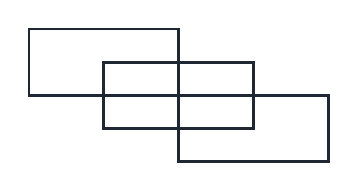
\begin{tikzpicture}[x=0.95cm,y=0.42cm]
\draw[Ink,line width=1pt] (0,2) rectangle (2,4);
\draw[Ink,line width=1pt] (1,1) rectangle (3,3);
\draw[Ink,line width=1pt] (2,0) rectangle (4,2);
\end{tikzpicture}
\end{minipage}
\end{probbox}
\probsol{
\textbf{Phân tích đề.} Ba hình chữ nhật bằng nhau, gọi là \textbf{I} (trên--trái), \textbf{II} (giữa) và \textbf{III} (dưới--phải). Các cạnh cắt nhau tạo ra thêm nhiều hình chữ nhật nhỏ. Ta phải đếm \emph{tất cả} các hình chữ nhật có đủ bốn cạnh được vẽ trên hình.
\step{1}{Quan sát kỹ hình vẽ}
Đặt tên các điểm như hình dưới. Để ý: cạnh dưới của hình I và cạnh trên của hình III nằm trên \emph{cùng một đường thẳng} và nối tiếp nhau tại điểm $O$ -- tâm của hình II. Tương tự cạnh phải của hình I và cạnh trái của hình III nối tiếp nhau tại $O$. Vì vậy bên trong hình II có một ``dấu cộng'' chia hình II thành $4$ ô nhỏ bằng nhau.
\begin{center}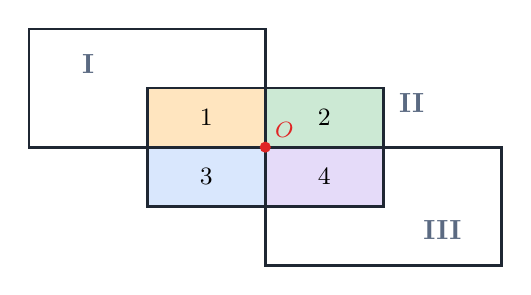
\begin{tikzpicture}[x=1.5cm,y=0.75cm,font=\sffamily\small]
\fill[tmOrange!25] (1,2) rectangle (2,3);\fill[tmGreen!25] (2,2) rectangle (3,3);
\fill[tmBlue!20] (1,1) rectangle (2,2);\fill[tmPurple!20] (2,1) rectangle (3,2);
\draw[Ink,line width=1pt] (0,2) rectangle (2,4);
\draw[Ink,line width=1pt] (1,1) rectangle (3,3);
\draw[Ink,line width=1pt] (2,0) rectangle (4,2);
\node at (1.5,2.5){$1$};\node at (2.5,2.5){$2$};\node at (1.5,1.5){$3$};\node at (2.5,1.5){$4$};
\fill[AnsRed] (2,2) circle (2pt);\node[above right,font=\footnotesize\bfseries,text=AnsRed] at (2,2){$O$};
\node[font=\bfseries,text=Slate] at (0.5,3.4){I};\node[font=\bfseries,text=Slate] at (3.5,0.6){III};
\node[font=\bfseries,text=Slate,anchor=west] at (3.05,2.75){II};
\end{tikzpicture}\end{center}
\step{2}{Đếm theo từng loại}
\begin{itemize}[leftmargin=1.2em,itemsep=1pt,topsep=1pt]
\item \textbf{Ba hình chữ nhật lớn ban đầu:} I, II, III -- $3$ hình.
\item \textbf{Bốn ô nhỏ} trong hình II (ô $1$, $2$, $3$, $4$) -- $4$ hình. Mỗi ô đều có đủ bốn cạnh: ví dụ ô $1$ có cạnh trên và cạnh trái là cạnh của hình II, cạnh dưới và cạnh phải là cạnh của hình I.
\item \textbf{Nửa hình II} (ghép hai ô cạnh nhau): ô $1+2$ (nửa trên), ô $3+4$ (nửa dưới), ô $1+3$ (nửa trái), ô $2+4$ (nửa phải) -- $4$ hình.
\end{itemize}
\step{3}{Kiểm tra không còn hình nào khác}
\begin{itemize}[leftmargin=1.2em,itemsep=1pt,topsep=1pt]
\item Phần của hình I nằm \emph{ngoài} hình II có dạng chữ L, và không có đoạn kẻ nào đi xuyên qua vùng đó. Một hình chữ nhật muốn chứa một phần vùng chữ L này thì phải lấy cạnh trái và cạnh trên của hình I làm cạnh của nó; hai cạnh này chỉ dài đúng bằng cạnh của hình I, nên hình chữ nhật đó chính là hình I. Tương tự, hình chữ nhật chứa một phần của III nằm ngoài II chỉ có thể là hình III.
\item Mọi hình chữ nhật còn lại phải nằm gọn trong hình II. Hình II cùng ``dấu cộng'' bên trong là một lưới $2\times2$ ô, và ở bước 2 ta đã kể đủ: $4$ ô, $4$ nửa và chính hình II.
\end{itemize}
\begin{warnbox}Đừng đếm hình chữ nhật lớn bao quanh cả ba hình (từ góc trên-trái của I đến góc dưới-phải của III): hình đó \emph{không} có cạnh nào được vẽ đầy đủ. Và cũng đừng bỏ sót các ô nhỏ do ``dấu cộng'' ở tâm tạo ra.\end{warnbox}
\step{4}{Cộng lại}
$3+4+4=11$ hình chữ nhật.
\verify{Đếm cách khác -- chỉ trong hình II (đây là một lưới $2\times2$ đầy đủ): theo Ví dụ 7 có $9$ hình chữ nhật (gồm $4$ ô, $4$ nửa và chính hình II). Cộng thêm hình I và hình III: $9+2=11$ \checkmark.}
Đáp án là \textbf{(A)}.
\ans{(A) $11$}
}

% ---------------- part b ----------------
% ================= Topic 3 (VI) -- part b: problems 16--30 =================
\providecommand{\cpTooth}[3]{% #1 rows, #2 columns, #3 unit (cm): grid of toothpicks
  \foreach \j in {0,...,#1}{\foreach \i in {1,...,#2}{
    \draw[tmOrange!85!black,line width=1.6pt,line cap=round]
      ({(\i-1)*#3+0.05},{\j*#3})--({\i*#3-0.05},{\j*#3});}}
  \foreach \j in {1,...,#1}{\foreach \i in {0,...,#2}{
    \draw[tmOrange!85!black,line width=1.6pt,line cap=round]
      ({\i*#3},{(\j-1)*#3+0.05})--({\i*#3},{\j*#3-0.05});}}}


\begin{probbox}{16}{\relax}
Trên lưới điểm ở hình bên, bạn Jane đứng ở điểm $A$. Jane tung một đồng xu cân đối để quyết định
cách di chuyển: nếu đồng xu ra mặt \emph{sấp} thì Jane đi \emph{lên} một điểm; nếu ra mặt \emph{ngửa}
thì Jane đi \emph{sang phải} một điểm. Sau đúng bốn lần tung, Jane sẽ dừng ở một trong năm điểm
$P$, $Q$, $R$, $S$, $T$. Xác suất để Jane dừng ở điểm $R$ là bao nhiêu?
\begin{figC}\begin{scope}[scale=0.8]
  \foreach \y in {0,...,4}{\pgfmathtruncatemacro\m{4-\y}
    \foreach \x in {0,...,\m}{\fill[Navy] (\x,\y) circle (2.6pt);}}
  \node[below left] at (0,0) {$A$};
  \node[above right] at (0,4) {$P$};\node[above right] at (1,3) {$Q$};
  \node[above right] at (2,2) {$R$};\node[above right] at (3,1) {$S$};
  \node[above right] at (4,0) {$T$};
  \fill[tmOrange] (0,0) circle (3.4pt);
\end{scope}\end{figC}
\choices{$\dfrac12$}{$\dfrac38$}{$\dfrac9{16}$}{$\dfrac7{16}$}{$\dfrac5{16}$}
\end{probbox}
\probsol{
\textbf{Phân tích đề.} Mỗi lần tung, Jane đi \emph{lên} ($\uparrow$, khi ra sấp) hoặc \emph{sang phải}
($\rightarrow$, khi ra ngửa). Sau $4$ lần tung, Jane đi đúng $4$ bước. Ta cần tính xác suất để
sau $4$ bước Jane đứng ở $R$.

\step{1}{Đếm tất cả các kết quả có thể}
Mỗi lần tung có $2$ kết quả (sấp hoặc ngửa), bốn lần tung liên tiếp cho
$2\times2\times2\times2=16$ dãy kết quả, ví dụ $\uparrow\rightarrow\rightarrow\uparrow$.
Vì đồng xu cân đối nên $16$ dãy này \emph{đồng khả năng}.
\begin{recallbox}\emph{Quy tắc nhân:} nếu việc thứ nhất có $a$ cách, việc thứ hai có $b$ cách, \dots{} thì
làm lần lượt các việc đó có $a\times b\times\cdots$ cách. \emph{Xác suất} của một biến cố (khi các kết
quả đồng khả năng) $=\dfrac{\text{số kết quả thuận lợi}}{\text{số kết quả có thể}}$.\end{recallbox}

\step{2}{Điểm cuối chỉ phụ thuộc vào số bước đi lên}
Nếu trong $4$ bước có $k$ bước đi lên thì có $4-k$ bước sang phải. Thứ tự các bước không làm thay
đổi điểm cuối. Đặt $A$ là gốc, ta có: $4$ lần lên $\to P$; $3$ lần lên $\to Q$;
$2$ lần lên $\to R$; $1$ lần lên $\to S$; $0$ lần lên $\to T$.
Vậy Jane dừng ở $R$ khi và chỉ khi có \textbf{đúng $2$ bước lên và $2$ bước sang phải}.

\step{3}{Liệt kê các dãy thuận lợi}
Ta chọn vị trí của hai bước $\uparrow$ trong bốn lượt (lượt 1, 2, 3, 4):
\[\uparrow\uparrow\rightarrow\rightarrow,\quad \uparrow\rightarrow\uparrow\rightarrow,\quad
\uparrow\rightarrow\rightarrow\uparrow,\quad \rightarrow\uparrow\uparrow\rightarrow,\quad
\rightarrow\uparrow\rightarrow\uparrow,\quad \rightarrow\rightarrow\uparrow\uparrow.\]
Có $6$ dãy (chọn $2$ lượt trong $4$ lượt: $\dfrac{4\times3}{2}=6$ cách).

\step{4}{Tính xác suất}
\[P(\text{dừng ở } R)=\frac{6}{16}=\frac38.\]

\step{5}{Một cách nhìn bằng hình: ghi số đường đi tới mỗi điểm}
Ghi vào mỗi điểm số dãy bước dẫn từ $A$ tới điểm đó. Mỗi điểm chỉ có thể tới từ điểm ngay bên trái hoặc
ngay bên dưới, nên số ở mỗi điểm $=$ tổng hai số ở bên trái và bên dưới (giống tam giác Pascal):
\begin{figC}\begin{scope}[scale=0.75]
  \foreach \x/\y/\n in {0/0/1,1/0/1,2/0/1,3/0/1,4/0/1,0/1/1,1/1/2,2/1/3,3/1/4,0/2/1,1/2/3,2/2/6,
     0/3/1,1/3/4,0/4/1}{
    \fill[tmBlue!12] (\x,\y) circle (9pt);
    \node[font=\small\bfseries,text=Navy] at (\x,\y) {\n};}
  \draw[AnsRed,thick] (2,2) circle (10pt);
  \node[right=10pt,text=AnsRed,font=\small] at (2,2) {$R$};
  \node[right=10pt,font=\small] at (4,0) {$T$};\node[right=10pt,font=\small] at (3,1) {$S$};
  \node[right=10pt,font=\small] at (1,3) {$Q$};\node[right=10pt,font=\small] at (0,4) {$P$};
\end{scope}\end{figC}
Trên đường chéo cuối: $1+4+6+4+1=16$ (đúng bằng tổng số dãy) và tại $R$ có số $6$.
\begin{warnbox}Năm điểm $P,Q,R,S,T$ \emph{không} đồng khả năng! Không được trả lời ``$1$ trong $5$ điểm nên
xác suất là $\frac15$''. Điểm ở giữa ($R$) có nhiều đường đi tới nhất; hai điểm ở đầu ($P$ và $T$) mỗi điểm chỉ có một đường.\end{warnbox}
\verify{Xác suất dừng ở các điểm $P,Q,R,S,T$ lần lượt là $\frac1{16},\frac4{16},\frac6{16},\frac4{16},\frac1{16}$;
tổng bằng $\frac{16}{16}=1$, hợp lý.}
Giá trị $\frac38=\frac6{16}$ là phương án \textbf{(B)}.
\ans{(B) $\dfrac38$}
}

\begin{probbox}{17}{\relax}
Người ta dùng các que tăm giống hệt nhau để xếp thành các lưới ô vuông như hình dưới. Chẳng hạn, lưới
$1\times10$ (gồm $1$ hàng, $10$ cột ô vuông) cần tất cả $31$ que tăm. Hỏi để xếp lưới $43\times10$
($43$ hàng, mỗi hàng $10$ ô) thì cần bao nhiêu que tăm?
\begin{figC}
  \begin{scope}[shift={(0,2.4)}]\cpTooth{1}{10}{0.42}\node[right] at (4.4,0.21) {$1\times10$};\end{scope}
  \begin{scope}[shift={(0,1.05)}]\cpTooth{2}{10}{0.42}\node[right] at (4.4,0.42) {$2\times10$};\end{scope}
  \begin{scope}[shift={(0,-0.6)}]\cpTooth{3}{10}{0.42}\node[right] at (4.4,0.63) {$3\times10$};\end{scope}
\end{figC}
\choices{$913$}{$860$}{$871$}{$903$}{$946$}
\end{probbox}
\probsol{
\textbf{Phân tích đề.} Lưới $43\times10$ có $43$ hàng ô vuông, mỗi hàng $10$ ô. Các que tăm nằm theo hai
hướng: \emph{nằm ngang} và \emph{thẳng đứng}. Ta đếm riêng từng loại rồi cộng lại (quy tắc cộng).

\step{1}{Kiểm tra cách đếm trên lưới $1\times10$}
\emph{Que nằm ngang:} lưới có $2$ đường kẻ ngang (cạnh trên và cạnh dưới), mỗi đường gồm $10$ que:
$2\times10=20$ que.
\emph{Que thẳng đứng:} có $11$ đường kẻ dọc ($10$ ô cần $11$ vách ngăn), mỗi đường gồm $1$ que:
$11\times1=11$ que. Tổng: $20+11=31$ que, đúng như đề cho.
\begin{recallbox}Một hàng có $10$ ô thì cần $10+1=11$ vách dọc (giống bài toán trồng cây: $10$ khoảng cách
thì có $11$ cây). Tương tự, $43$ hàng ô thì có $43+1=44$ đường kẻ ngang.\end{recallbox}

\step{2}{Đếm que nằm ngang của lưới $43\times10$}
Có $43+1=44$ đường kẻ ngang, mỗi đường dài $10$ que: $44\times10=440$ que.

\step{3}{Đếm que thẳng đứng của lưới $43\times10$}
Có $10+1=11$ đường kẻ dọc, mỗi đường dài $43$ que (mỗi hàng ô góp $1$ que): $11\times43=473$ que.

\step{4}{Cộng lại}
$440+473=913$ que tăm.

\step{5}{Cách thứ hai: thêm từng hàng}
Lưới $1\times10$ có $31$ que. Mỗi khi đặt thêm một hàng mới lên trên, ta cần thêm $10$ que nằm ngang
(cạnh trên của hàng mới) và $11$ que thẳng đứng, tức $21$ que (cạnh dưới đã có sẵn). Từ $1$ hàng lên
$43$ hàng phải thêm $42$ hàng:
\[31+42\times21=31+882=913.\]
\begin{warnbox}Không được lấy $43\times31=1333$: khi chồng các hàng lên nhau, hai hàng kề nhau \emph{dùng chung}
một dãy $10$ que nằm ngang, nên nhân như vậy là đếm trùng.\end{warnbox}
\verify{Theo công thức $(\text{số hàng}+1)\times10+11\times\text{số hàng}$: lưới $2\times10$ cần
$3\times10+11\times2=52$ que, lưới $3\times10$ cần $4\times10+11\times3=73$ que; đếm trực tiếp trên hình cũng
được $52$ và $73$. Hai cách tính cho cùng kết quả $913$.}
Vậy chọn \textbf{(A)}.
\ans{(A) $913$ que tăm}
}

\begin{probbox}{18}{\relax}
Ở căng-tin trường bạn Braydon, món thịt có hai loại là thịt bò và thịt gà; trái cây có ba loại là táo, lê
và chuối. Braydon được phát ngẫu nhiên một suất ăn gồm một món thịt và một loại trái cây. Xác suất để
suất ăn của Braydon có chuối là
\choices{$\dfrac13$}{$\dfrac23$}{$\dfrac12$}{$\dfrac15$}{$\dfrac35$}
\end{probbox}
\probsol{
\textbf{Phân tích đề.} Một suất ăn $=$ (một món thịt, một loại trái cây). Suất ăn được chọn ngẫu nhiên
nên mọi suất ăn có thể đều đồng khả năng. Cần tìm xác suất suất ăn có chuối.

\step{1}{Liệt kê tất cả các suất ăn có thể}
Theo quy tắc nhân có $2\times3=6$ suất ăn. Ta lập bảng (hàng: thịt, cột: trái cây):
\begin{center}\begin{tabular}{|c|c|c|c|}\hline
 & Táo & Lê & \cellcolor{tmOrange!20}Chuối\\\hline
Bò & Bò--Táo & Bò--Lê & \cellcolor{tmOrange!20}Bò--Chuối\\\hline
Gà & Gà--Táo & Gà--Lê & \cellcolor{tmOrange!20}Gà--Chuối\\\hline
\end{tabular}\end{center}

\step{2}{Đếm các suất ăn có chuối}
Cột ``Chuối'' có $2$ suất: Bò--Chuối và Gà--Chuối.

\step{3}{Tính xác suất}
\[P(\text{có chuối})=\frac{2}{6}=\frac13.\]
\begin{recallbox}Rút gọn phân số: chia cả tử và mẫu cho ước chung lớn nhất: $\dfrac26=\dfrac{2:2}{6:2}=\dfrac13$.\end{recallbox}
\begin{tipbox}Món thịt không ảnh hưởng gì tới trái cây. Có thể nghĩ gọn: trái cây được chọn là một trong
$3$ loại đồng khả năng, chuối là $1$ trong $3$ loại, nên xác suất là $\frac13$.\end{tipbox}
\begin{warnbox}Đừng cộng ``$2$ loại thịt $+\,3$ loại trái cây $=5$'' rồi trả lời $\frac15$: số suất ăn là
$2\times3=6$ chứ không phải $2+3=5$.\end{warnbox}
\verify{Xác suất có táo, có lê, có chuối đều bằng $\frac13$; tổng $\frac13+\frac13+\frac13=1$.}
Vậy chọn \textbf{(A)}.
\ans{(A) $\dfrac13$}
}

\begin{probbox}{19}{\relax}
Người ta làm một con xúc xắc đặc biệt có sáu mặt, mỗi mặt ghi một số (các số có thể trùng nhau). Khi gieo
xúc xắc này, xác suất được một số chia hết cho $3$ là $\frac12$, còn xác suất được một số chẵn là $\frac13$.
Sáu số trên các mặt có thể là
\choicesII{$1,2,3,5,5,6$}{$1,2,3,3,5,6$}{$1,2,3,4,6,6$}{$1,2,3,3,4,6$}{$2,3,3,3,5,6$}
\end{probbox}
\probsol{
\textbf{Phân tích đề.} Xúc xắc có $6$ mặt đồng khả năng. Từ hai xác suất đã cho, ta suy ra \emph{số mặt}
ghi số chia hết cho $3$ và số mặt ghi số chẵn, rồi kiểm tra từng phương án.

\step{1}{Đổi xác suất thành số mặt}
\begin{recallbox}Với $6$ mặt đồng khả năng: $P=\dfrac{\text{số mặt thuận lợi}}{6}$, nên
số mặt thuận lợi $=P\times6$.\end{recallbox}
Số mặt chia hết cho $3$: $\frac12\times6=3$ mặt.\quad Số mặt chẵn: $\frac13\times6=2$ mặt.

Vậy ta cần: \textbf{đúng $3$ mặt chia hết cho $3$} và \textbf{đúng $2$ mặt chẵn}.

\step{2}{Kiểm tra từng phương án}
Trong các số từ $1$ đến $6$: các số chia hết cho $3$ là $3$ và $6$; các số chẵn là $2$, $4$, $6$.
Chú ý số $6$ vừa chẵn vừa chia hết cho $3$, nên phải đếm nó ở \emph{cả hai} cột.
\begin{center}\begin{tabular}{|c|c|c|c|c|}\hline
Phương án & Các mặt & Mặt chia hết cho $3$ & Mặt chẵn & Đạt?\\\hline
(A) & $1,2,3,5,5,6$ & $3,6$ \;($2$ mặt) & $2,6$ \;($2$ mặt) & Không\\\hline
\rowcolor{tmGreen!12}(B) & $1,2,3,3,5,6$ & $3,3,6$ \;($3$ mặt) & $2,6$ \;($2$ mặt) & Có\\\hline
(C) & $1,2,3,4,6,6$ & $3,6,6$ \;($3$ mặt) & $2,4,6,6$ \;($4$ mặt) & Không\\\hline
(D) & $1,2,3,3,4,6$ & $3,3,6$ \;($3$ mặt) & $2,4,6$ \;($3$ mặt) & Không\\\hline
(E) & $2,3,3,3,5,6$ & $3,3,3,6$ \;($4$ mặt) & $2,6$ \;($2$ mặt) & Không\\\hline
\end{tabular}\end{center}
\begin{warnbox}Quên rằng $6$ là số chẵn thì sẽ đếm sai số mặt chẵn của (D) thành $2$ và chọn nhầm (D).\end{warnbox}
\verify{Với (B): $P(\text{chia hết cho }3)=\frac36=\frac12$, $P(\text{chẵn})=\frac26=\frac13$. Chỉ có phương án \textbf{(B)} thoả mãn.}
\ans{(B) $1,2,3,3,5,6$}
}


\begin{probbox}{20}{\stars{1}}
Ba tuyến xe buýt chạy trên các con đường như hình vẽ, cùng đi qua bến $X$ (các đoạn có cùng số vạch
nhỏ thì dài bằng nhau: $PX=XS$, $QX=XT$, $RX=XU$).
\begin{itemize}[leftmargin=1.2em,itemsep=1pt,topsep=2pt]
\item Xe $A$ chạy theo lộ trình $P\to X\to S\to X\to P$, mỗi vòng mất $12$ phút.
\item Xe $B$ chạy theo lộ trình $Q\to X\to T\to X\to Q$, mỗi vòng mất $20$ phút.
\item Xe $C$ chạy theo lộ trình $R\to X\to U\to X\to R$, mỗi vòng mất $28$ phút.
\end{itemize}
Lúc $13$\,h, ba xe $A$, $B$, $C$ lần lượt xuất phát từ $P$, $Q$, $R$. Mỗi xe chạy với vận tốc không đổi,
quay đầu ngay lập tức ở hai đầu lộ trình và chạy liên tục đến $23$\,h. Hỏi trong khoảng thời gian từ
$17$\,h đến $22$\,h, có bao nhiêu thời điểm mà có từ hai xe trở lên cùng có mặt tại bến $X$?
\begin{figC}\begin{scope}[scale=0.9]
  \draw[Ink,thick] (0,1.6)--(0,-1.6);\draw[Ink,thick] (-1.9,0)--(1.9,0);\draw[Ink,thick] (-2,-1.35)--(2,1.35);
  \foreach \p in {(0,1.6),(0,-1.6),(-1.9,0),(1.9,0),(-2,-1.35),(2,1.35),(0,0)}{\fill[Navy] \p circle (2pt);}
  \node[above] at (0,1.6) {$P$};\node[below] at (0,-1.6) {$S$};\node[left] at (-1.9,0) {$Q$};
  \node[right] at (1.9,0) {$T$};\node[below left] at (-2,-1.35) {$R$};\node[above right] at (2,1.35) {$U$};
  \node[below right] at (0.05,-0.02) {$X$};
  % ticks
  \draw[tmBlue,thick] (-0.12,0.8)--(0.12,0.8);\draw[tmBlue,thick] (-0.12,-0.8)--(0.12,-0.8);
  \foreach \s in {-1,1}{\draw[tmOrange,thick] (\s*0.95-0.04,-0.12)--(\s*0.95-0.04,0.12);
                        \draw[tmOrange,thick] (\s*0.95+0.04,-0.12)--(\s*0.95+0.04,0.12);}
  \foreach \s in {-1,1}{\foreach \d in {-0.09,0,0.09}{
     \draw[tmGreen!80!black,thick] ($(\s*1,\s*0.675)+(\d*0.829,\d*0.559)+(0.067,-0.1)$)--++(-0.134,0.2);}}
\end{scope}\end{figC}
\choices{$18$}{$19$}{$20$}{$21$}{$22$}
\end{probbox}
\probsol{
\textbf{Phân tích đề.} Ta đo thời gian bằng \emph{số phút kể từ $13$\,h} và gọi số đó là $t$. Cần tìm
những giá trị $t$ mà có ít nhất hai xe cùng ở $X$, với $t$ nằm trong khoảng từ $17$\,h đến $22$\,h.

\step{1}{Đổi khoảng thời gian cần xét ra số phút}
$17$\,h là $4$ giờ sau $13$\,h: $t=4\times60=240$. \quad $22$\,h là $9$ giờ sau $13$\,h: $t=9\times60=540$.
Vậy ta xét $240\le t\le540$.

\step{2}{Xe $A$ có mặt ở $X$ vào những lúc nào?}
Một vòng của xe $A$ gồm $4$ đoạn bằng nhau: $P\to X$, $X\to S$, $S\to X$, $X\to P$ (vì $PX=XS$).
Xe chạy đều nên mỗi đoạn mất $12:4=3$ phút. Xe $A$ tới $X$ ở cuối đoạn thứ nhất và cuối đoạn thứ ba
của mỗi vòng, tức là lúc
\[t=3,\ 9,\ 15,\ 21,\ 27,\ \dots\]
Đó chính là các \textbf{bội lẻ của $3$} ($3\times1$, $3\times3$, $3\times5$, \dots). Ở cuối đoạn thứ hai và thứ tư
xe ở $S$ hoặc $P$, không ở $X$.

\step{3}{Tương tự với xe $B$ và xe $C$}
Xe $B$: mỗi đoạn mất $20:4=5$ phút, xe ở $X$ lúc $t=5,15,25,35,\dots$ -- các \textbf{bội lẻ của $5$}.\\
Xe $C$: mỗi đoạn mất $28:4=7$ phút, xe ở $X$ lúc $t=7,21,35,49,\dots$ -- các \textbf{bội lẻ của $7$}.

\step{4}{Khi nào hai xe gặp nhau ở $X$?}
\begin{recallbox}Một số chia hết cho cả $3$ và $5$ thì chia hết cho $\text{BCNN}(3,5)=15$. Tương tự:
chia hết cho cả $3$ và $7$ $\Leftrightarrow$ chia hết cho $21$; chia hết cho cả $5$ và $7$ $\Leftrightarrow$
chia hết cho $35$.\end{recallbox}
Xe $A$ và xe $B$ cùng ở $X$ khi $t$ vừa là bội lẻ của $3$ vừa là bội lẻ của $5$, tức $t$ là \textbf{số lẻ chia hết cho $15$}
(bội lẻ của $15$). Tương tự: $A$ và $C$ gặp nhau khi $t$ là bội lẻ của $21$; $B$ và $C$ gặp nhau khi $t$ là bội lẻ của $35$.
\begin{proofbox}Bội lẻ của $15$ là số lẻ chia hết cho $15$, nên nó vừa là số lẻ chia hết cho $3$ (bội lẻ của $3$), vừa là
số lẻ chia hết cho $5$ (bội lẻ của $5$). Ngược lại, một số vừa là bội lẻ của $3$ vừa là bội lẻ của $5$ thì lẻ và chia
hết cho $15$.\end{proofbox}

\step{5}{Liệt kê trong khoảng $240\le t\le540$}
\begin{center}\begin{tabular}{|l|l|c|}\hline
Hai xe & Các giá trị $t$ (bội lẻ) & Số lần\\\hline
$A$ và $B$ ($15$) & $255, 285, 315, 345, 375, 405, 435, 465, 495, 525$ & $10$\\\hline
$A$ và $C$ ($21$) & $273, 315, 357, 399, 441, 483, 525$ & $7$\\\hline
$B$ và $C$ ($35$) & $245, 315, 385, 455, 525$ & $5$\\\hline
\end{tabular}\end{center}
(Ví dụ hàng đầu: $15\times17=255$ là bội lẻ đầu tiên lớn hơn $240$; sau đó cứ cộng thêm $30$, vì giữa hai
bội lẻ liên tiếp của $15$ cách nhau $2\times15=30$.)

\step{6}{Bỏ các thời điểm bị đếm trùng}
Cộng ba hàng được $10+7+5=22$, nhưng các thời điểm $315$ và $525$ xuất hiện ở \emph{cả ba hàng}
(đó là bội lẻ của $3\times5\times7=105$: lúc ấy cả ba xe cùng ở $X$). Mỗi thời điểm này bị đếm $3$ lần
trong khi chỉ được đếm $1$ lần, nên phải bớt $2+2=4$:
\[22-4=18 \text{ thời điểm.}\]
\begin{warnbox}Đề hỏi số \emph{thời điểm}, không phải số ``cặp xe gặp nhau''. Lúc ba xe cùng ở $X$ chỉ là
\emph{một} thời điểm. Cộng thẳng $10+7+5=22$ rồi chọn (E) là sai.\end{warnbox}
\verify{Đổi ra giờ: $17$\,h\,05; $17$\,h\,15; $17$\,h\,33; $17$\,h\,45; $18$\,h\,15; $18$\,h\,45; $18$\,h\,57;
$19$\,h\,15; $19$\,h\,25; $19$\,h\,39; $19$\,h\,45; $20$\,h\,15; $20$\,h\,21; $20$\,h\,35; $20$\,h\,45; $21$\,h\,03;
$21$\,h\,15; $21$\,h\,45 -- đếm được đúng $18$ thời điểm, tất cả đều nằm giữa $17$\,h và $22$\,h.}
Vậy chọn \textbf{(A)}.
\ans{(A) $18$}
}

\begin{probbox}{21}{\relax}
Mỗi mặt của một hình lập phương được sơn đúng một màu. Cần ít nhất bao nhiêu màu để sơn hình lập
phương sao cho hai mặt bất kì có chung một cạnh thì có màu khác nhau?
\choices{$2$}{$3$}{$4$}{$5$}{$6$}
\end{probbox}
\probsol{
\textbf{Phân tích đề.} Hai mặt ``có chung một cạnh'' là hai mặt kề nhau. Hai mặt đối diện (như mặt trên và
mặt dưới) không có cạnh chung nên được phép cùng màu. Ta cần (1) chỉ ra một cách tô dùng ít màu, và
(2) chứng minh không thể dùng ít màu hơn.

\step{1}{Hai màu là không đủ}
\begin{proofbox}Xét một đỉnh bất kì của hình lập phương, chẳng hạn đỉnh trên--trước--phải. Có ba mặt gặp nhau ở
đỉnh đó: mặt trên, mặt trước, mặt phải. Hai mặt bất kì trong ba mặt này đều có chung một cạnh, nên ba mặt
này phải có ba màu đôi một khác nhau. Do đó cần ít nhất $3$ màu.\end{proofbox}

\step{2}{Ba màu là đủ}
Tô \emph{hai mặt đối diện cùng một màu}: mặt trên và mặt dưới màu xanh dương, mặt trước và mặt sau màu
cam, mặt trái và mặt phải màu xanh lá. Mỗi mặt kề với $4$ mặt, đó chính là bốn mặt \emph{không} đối diện
với nó, và bốn mặt này mang hai màu kia. Vậy không có hai mặt kề nhau nào cùng màu.
\begin{figC}
  \begin{scope}
   \fill[tmOrange!55,draw=Ink,thick] (0,0)--(1.6,0)--(1.6,1.6)--(0,1.6)--cycle;
   \fill[tmBlue!55,draw=Ink,thick] (0,1.6)--(1.6,1.6)--(2.4,2.3)--(0.8,2.3)--cycle;
   \fill[tmGreen!55,draw=Ink,thick] (1.6,0)--(2.4,0.7)--(2.4,2.3)--(1.6,1.6)--cycle;
   \node at (0.8,0.8) {trước};\node at (1.2,1.95) {trên};\node[rotate=0] at (2,1.15) {phải};
  \end{scope}
  \begin{scope}[shift={(4,0.1)},scale=0.5]
   \foreach \x/\y/\c in {1/2/tmBlue,0/1/tmGreen,1/1/tmOrange,2/1/tmGreen,3/1/tmOrange,1/0/tmBlue}{
     \fill[\c!55,draw=Ink,thick] (\x,\y) rectangle ++(1,1);}
   \node[font=\scriptsize] at (2,-0.45) {hình khai triển};
  \end{scope}
\end{figC}

\step{3}{Kết luận}
Cần ít nhất $3$ màu (bước 1) và $3$ màu là đủ (bước 2), nên số màu nhỏ nhất là $3$.
\begin{warnbox}Chỉ tìm được một cách tô bằng $3$ màu thì \emph{chưa đủ} để khẳng định $3$ là nhỏ nhất; phải
giải thích vì sao $2$ màu không được (lập luận ba mặt chung đỉnh). Ngược lại, nghĩ rằng ``$6$ mặt phải có
$6$ màu'' là quên rằng mặt đối diện được phép cùng màu.\end{warnbox}
\verify{Trên hình khai triển, mỗi ô vuông chỉ chung cạnh với các ô khác màu (khi gấp lại, hai ô cùng màu
là hai mặt đối diện).}
Vậy chọn \textbf{(B)}.
\ans{(B) $3$ màu}
}

\begin{probbox}{22}{\relax}
Có bao nhiêu cặp số $(m,n)$ khác nhau lấy từ các số nguyên $1,2,3,\dots,20$ sao cho $m<n$ và $m+n$ là số chẵn?
\choices{$55$}{$90$}{$140$}{$110$}{$50$}
\end{probbox}
\probsol{
\textbf{Phân tích đề.} Ta chọn hai số khác nhau trong $20$ số; vì yêu cầu $m<n$ nên mỗi cặp hai số chỉ được
đếm \emph{một lần} (số nhỏ là $m$, số lớn là $n$). Điều kiện: tổng $m+n$ chẵn.

\step{1}{Khi nào tổng hai số là số chẵn?}
\begin{recallbox}chẵn $+$ chẵn $=$ chẵn;\quad lẻ $+$ lẻ $=$ chẵn;\quad chẵn $+$ lẻ $=$ lẻ.\end{recallbox}
Vậy $m+n$ chẵn khi và chỉ khi $m$ và $n$ \textbf{cùng tính chẵn lẻ} (cùng chẵn hoặc cùng lẻ).

\step{2}{Chia $20$ số thành hai nhóm}
Nhóm chẵn: $2,4,6,\dots,20$ -- có $10$ số.\quad Nhóm lẻ: $1,3,5,\dots,19$ -- có $10$ số.

\step{3}{Đếm số cặp trong nhóm chẵn}
Chọn số thứ nhất có $10$ cách, số thứ hai (khác số thứ nhất) có $9$ cách: $10\times9=90$ cách chọn \emph{có thứ tự}.
Nhưng mỗi cặp, ví dụ $\{2,4\}$, bị đếm hai lần ($2$ rồi $4$, hoặc $4$ rồi $2$), trong khi điều kiện $m<n$
chỉ cho phép một thứ tự $(2,4)$. Vậy số cặp là $\dfrac{10\times9}{2}=45$.
\begin{recallbox}Số cách chọn $2$ phần tử (không kể thứ tự) từ $k$ phần tử là $\dfrac{k\times(k-1)}{2}$.\end{recallbox}

\step{4}{Đếm số cặp trong nhóm lẻ và cộng lại}
Tương tự, nhóm lẻ cho $45$ cặp. Một cặp không thể vừa ở nhóm chẵn vừa ở nhóm lẻ, nên theo quy tắc cộng:
$45+45=90$ cặp.
\begin{warnbox}Quên chia cho $2$ sẽ được $90+90=180$ (không có trong đáp án); quên mất nhóm lẻ sẽ được
$45$. Hãy luôn tự hỏi: ``Mình có đếm một cặp hai lần không? Mình có bỏ sót trường hợp nào không?''\end{warnbox}
\verify{Đếm bằng phần bù: tổng số cặp $m<n$ là $\dfrac{20\times19}{2}=190$. Số cặp khác tính chẵn lẻ (một chẵn, một lẻ) là
$10\times10=100$. Vậy số cặp cùng tính chẵn lẻ là $190-100=90$. Khớp!}
Vậy chọn \textbf{(B)}.
\ans{(B) $90$ cặp}
}

\begin{probbox}{23}{\stars{1}}
Hai số nguyên dương có hai chữ số, khác nhau, được gọi là một \emph{cặp số đảo} nếu số này nhận được từ số kia bằng
cách đổi chỗ hai chữ số. Ví dụ: $52$ và $25$ là một cặp số đảo. Số $2015$ có một tính chất đặc biệt: nó bằng
tích của ba số nguyên tố khác nhau, trong đó có hai số tạo thành một cặp số đảo ($2015=5\times13\times31$).
Kể cả $2015$, có bao nhiêu số nguyên dương nhỏ hơn $10\,000$ có cùng tính chất này?
\choices{$18$}{$14$}{$20$}{$17$}{$19$}
\end{probbox}
\probsol{
\textbf{Phân tích đề.} Ta cần đếm các số $N<10\,000$ có dạng $N=p\times q\times r$, với $p,q,r$ là ba số nguyên
tố khác nhau, trong đó hai số (gọi là $p$ và $q$) là một cặp số đảo có hai chữ số. Kế hoạch: tìm tất cả các
cặp số đảo gồm hai số nguyên tố, rồi với mỗi cặp tìm các số nguyên tố thứ ba phù hợp.

\step{1}{Tìm các cặp số đảo mà cả hai số đều là số nguyên tố}
\begin{recallbox}Số nguyên tố là số tự nhiên lớn hơn $1$ chỉ có hai ước là $1$ và chính nó. Các số nguyên tố có
hai chữ số: $11$, $13$, $17$, $19$, $23$, $29$, $31$, $37$, $41$, $43$, $47$, $53$, $59$, $61$, $67$, $71$, $73$, $79$, $83$, $89$, $97$.\end{recallbox}
\begin{tipbox}Số đảo của $p$ có chữ số hàng đơn vị chính là chữ số hàng chục của $p$. Số nguyên tố có hai chữ số
phải tận cùng bằng $1,3,7$ hoặc $9$, nên chỉ cần xét các số nguyên tố bắt đầu bằng $1,3,7,9$:
$11,13,17,19,31,37,71,73,79,97$.\end{tipbox}
Kiểm tra số đảo của từng số:
\begin{center}\begin{tabular}{|c|c|c|c|c|c|c|c|c|c|c|}\hline
$p$ & $11$ & $13$ & $17$ & $19$ & $31$ & $37$ & $71$ & $73$ & $79$ & $97$\\\hline
số đảo & $11$ & $31$ & $71$ & $91$ & $13$ & $73$ & $17$ & $37$ & $97$ & $79$\\\hline
nguyên tố? & trùng & có & có & không & có & có & có & có & có & có\\\hline
\end{tabular}\end{center}
($91=7\times13$ không là số nguyên tố; $11$ đảo lại vẫn là $11$, không phải hai số \emph{khác nhau}.)
Vậy có đúng $4$ cặp: $\{13,31\}$, $\{17,71\}$, $\{37,73\}$, $\{79,97\}$.

\step{2}{Tính tích của mỗi cặp}
$13\times31=403$;\quad $17\times71=1207$;\quad $37\times73=2701$;\quad $79\times97=7663$.

\step{3}{Tìm số nguyên tố thứ ba $r$ cho từng cặp}
Cần $r$ là số nguyên tố, khác hai số của cặp, và tích $<10\,000$.
\begin{itemize}[leftmargin=1.2em,itemsep=1pt,topsep=2pt]
\item Cặp $\{13,31\}$: cần $403\times r<10\,000$. Vì $403\times24=9672$ và $403\times25=10\,075$ nên $r\le23$.
Các số nguyên tố $\le23$ là $2,3,5,7,11,13,17,19,23$; bỏ $13$ (đã có trong cặp): còn $8$ số, cho
$806;\ 1209;\ 2015;\ 2821;\ 4433;\ 6851;\ 7657;\ 9269$.
\item Cặp $\{17,71\}$: cần $1207\times r<10\,000$, mà $1207\times8=9656$, $1207\times9=10\,863$ nên $r\le8$:
$r\in\{2,3,5,7\}$, cho $2414;\ 3621;\ 6035;\ 8449$ ($4$ số).
\item Cặp $\{37,73\}$: $2701\times3=8103<10\,000$, $2701\times4>10\,000$ nên $r\in\{2,3\}$: $5402;\ 8103$ ($2$ số).
\item Cặp $\{79,97\}$: ngay cả $7663\times2=15\,326>10\,000$, nên không có số nào.
\end{itemize}

\step{4}{Kiểm tra không có số nào bị đếm hai lần và cộng lại}
\begin{proofbox}Mỗi số chỉ có một cách phân tích ra thừa số nguyên tố. Nếu một số xuất hiện ở hai danh sách thì
trong ba thừa số nguyên tố của nó có hai cặp số đảo khác nhau; hai cặp này phải dùng chung một số nguyên tố.
Nhưng nhìn bảng ở bước 1, mỗi số nguyên tố chỉ thuộc đúng một cặp. Vậy không có số nào bị đếm hai lần.\end{proofbox}
Tổng cộng: $8+4+2+0=14$ số, ứng với phương án \textbf{(B)}.
\begin{warnbox}Hai lỗi hay gặp: (1) quên rằng số thứ ba phải \emph{khác} hai số của cặp, nên đếm thêm
$403\times13=5239=13\times13\times31$ (sai, vì $13$ lặp lại); (2) quên số nguyên tố $2$.\end{warnbox}
\verify{$2015=403\times5$ có trong danh sách; số lớn nhất $9269=13\times31\times23$ vẫn nhỏ hơn $10\,000$.}
\ans{(B) $14$}
}

\begin{probbox}{24}{\relax}
Hình bên được ghép từ $8$ hình bình hành nhỏ giống hệt nhau. Kể cả $8$ hình bình hành nhỏ đó, trong
hình có tất cả bao nhiêu hình bình hành?
\begin{figC}
  \foreach \j in {0,1,2}{\draw[Ink,thick] (\j*0.55,\j*0.8)--(4.4+\j*0.55,\j*0.8);}
  \foreach \i in {0,...,4}{\draw[Ink,thick] (\i*1.1,0)--(\i*1.1+1.1,1.6);}
\end{figC}
\choices{$29$}{$30$}{$26$}{$27$}{$28$}
\end{probbox}
\probsol{
\textbf{Phân tích đề.} Hình gồm $2$ hàng, mỗi hàng $4$ hình bình hành nhỏ. Mỗi hình bình hành trong hình được
tạo bởi các đoạn thẳng có sẵn: hai cạnh nằm trên \emph{đường nằm ngang}, hai cạnh nằm trên \emph{đường xiên}.

\step{1}{Đếm các đường thẳng của hình}
Đánh số: có $3$ đường nằm ngang (đáy, giữa, trên) và $5$ đường xiên (song song với nhau).
\begin{figC}
  \fill[tmGreen!30] (1.1,0)--(3.3,0)--(3.85,0.8)--(1.65,0.8)--cycle;
  \foreach \j/\l in {0/1,1/2,2/3}{\draw[tmBlue,thick] (\j*0.55,\j*0.8)--(4.4+\j*0.55,\j*0.8);
     \node[left,text=tmBlue,font=\scriptsize] at (\j*0.55,\j*0.8) {ngang \l};}
  \foreach \i in {0,...,4}{\draw[tmOrange,thick] (\i*1.1,0)--(\i*1.1+1.1,1.6);
     \pgfmathtruncatemacro\k{\i+1}\node[below,text=tmOrange!80!black,font=\scriptsize] at (\i*1.1,0) {x\k};}
\end{figC}
Ví dụ: hình bình hành tô xanh lá được xác định bởi đường ngang $1$, ngang $2$ và đường xiên x$2$, x$4$.

\step{2}{Mỗi hình bình hành ứng với một cách chọn $2$ đường ngang và $2$ đường xiên}
Chọn $2$ trong $3$ đường ngang làm cạnh dưới và cạnh trên, chọn $2$ trong $5$ đường xiên làm cạnh trái và cạnh phải,
ta được đúng một hình bình hành; ngược lại mỗi hình bình hành trong hình cho đúng một cách chọn như vậy.
\begin{recallbox}Số cách chọn $2$ đường trong $k$ đường là $\dfrac{k\times(k-1)}{2}$.\end{recallbox}
Chọn $2$ đường ngang: $\dfrac{3\times2}{2}=3$ cách. \quad Chọn $2$ đường xiên: $\dfrac{5\times4}{2}=10$ cách.

\step{3}{Áp dụng quy tắc nhân}
Số hình bình hành: $3\times10=30$.

\step{4}{Kiểm tra bằng cách đếm theo kích thước}
Gọi hình bình hành ``cao $a$, rộng $b$'' là hình gồm $a$ hàng và $b$ cột hình nhỏ:
\begin{center}\begin{tabular}{|c|c|c|c|c|c|}\hline
 & rộng $1$ & rộng $2$ & rộng $3$ & rộng $4$ & Cộng\\\hline
cao $1$ (có $2$ vị trí theo hàng) & $2\times4=8$ & $2\times3=6$ & $2\times2=4$ & $2\times1=2$ & $20$\\\hline
cao $2$ (có $1$ vị trí theo hàng) & $4$ & $3$ & $2$ & $1$ & $10$\\\hline
\end{tabular}\end{center}
\begin{warnbox}Đừng chỉ đếm $8$ hình nhỏ cộng vài hình lớn ``dễ thấy''. Hãy đếm có hệ thống: theo kích thước
(bảng trên) hoặc theo cách chọn các đường thẳng.\end{warnbox}
\verify{Tổng theo bảng: $20+10=30$, trùng với cách tính $3\times10$.}
Vậy chọn \textbf{(B)}.
\ans{(B) $30$ hình bình hành}
}

\begin{probbox}{25}{\stars{1}}
Trong một cái lọ có $2$ viên bi đỏ và $2$ viên bi xanh, ngoài ra không có viên bi nào khác. Bạn Angie lấy ngẫu
nhiên cùng lúc $2$ viên bi từ lọ. Nếu hai viên cùng màu, Angie bỏ ra ngoài một viên và trả viên kia vào lọ.
Nếu hai viên khác màu, Angie bỏ viên bi đỏ ra ngoài và trả viên bi xanh vào lọ. Angie làm như vậy tất cả ba lần.
Xác suất để viên bi cuối cùng còn lại trong lọ là bi đỏ bằng
\choices{$\dfrac12$}{$\dfrac14$}{$\dfrac23$}{$\dfrac13$}{$0$}
\end{probbox}
\probsol{
\textbf{Phân tích đề.} Mỗi lần lấy, trong lọ bớt đi đúng $1$ viên bi. Sau $3$ lần, từ $4$ viên còn lại $1$ viên.
Ta theo dõi \emph{trạng thái} của lọ, viết (số bi đỏ, số bi xanh), bắt đầu từ $(2\text{Đ},2\text{X})$.

\step{1}{Lần lấy thứ nhất, từ $(2\text{Đ},2\text{X})$}
Gọi các bi là Đ$_1$, Đ$_2$, X$_1$, X$_2$. Có $6$ cách lấy $2$ viên, đồng khả năng:
Đ$_1$Đ$_2$;\ X$_1$X$_2$;\ Đ$_1$X$_1$;\ Đ$_1$X$_2$;\ Đ$_2$X$_1$;\ Đ$_2$X$_2$.
\begin{itemize}[leftmargin=1.2em,itemsep=1pt,topsep=2pt]
\item Hai bi đỏ ($1$ cách): bỏ $1$ bi đỏ $\to(1\text{Đ},2\text{X})$.
\item Hai bi xanh ($1$ cách): bỏ $1$ bi xanh $\to(2\text{Đ},1\text{X})$.
\item Khác màu ($4$ cách): bỏ bi đỏ $\to(1\text{Đ},2\text{X})$.
\end{itemize}
Vậy sau lần $1$: trạng thái $(1\text{Đ},2\text{X})$ với xác suất $\frac56$, trạng thái $(2\text{Đ},1\text{X})$ với xác suất $\frac16$.

\step{2}{Lần lấy thứ hai}
Từ $(1\text{Đ},2\text{X})$: có $3$ cách lấy; $2$ cách khác màu $\to(0\text{Đ},2\text{X})$; $1$ cách hai bi xanh $\to(1\text{Đ},1\text{X})$.\\
Từ $(2\text{Đ},1\text{X})$: có $3$ cách lấy; $1$ cách hai bi đỏ $\to(1\text{Đ},1\text{X})$; $2$ cách khác màu $\to(1\text{Đ},1\text{X})$.
Vậy từ $(2\text{Đ},1\text{X})$ chắc chắn sang $(1\text{Đ},1\text{X})$.

\step{3}{Lần lấy thứ ba}
Từ $(0\text{Đ},2\text{X})$: lấy hai bi xanh, bỏ một $\to(0\text{Đ},1\text{X})$.\\
Từ $(1\text{Đ},1\text{X})$: lấy hai bi khác màu, bỏ bi đỏ $\to(0\text{Đ},1\text{X})$.
\begin{figC}
  \tikzset{st/.style={draw=tmBlue,fill=tmBlue!8,rounded corners=3pt,inner sep=3pt,font=\footnotesize}}
  \node[st] (a) at (0,0) {$2$Đ, $2$X};
  \node[st] (b) at (2.8,0.9) {$1$Đ, $2$X};\node[st] (c) at (2.8,-0.9) {$2$Đ, $1$X};
  \node[st] (d) at (5.6,0.9) {$0$Đ, $2$X};\node[st] (e) at (5.6,-0.9) {$1$Đ, $1$X};
  \node[st,draw=AnsRed,fill=AnsRed!8] (f) at (8.2,0) {$0$Đ, $1$X};
  \draw[->,thick,Slate] (a)--node[above,font=\scriptsize]{$\frac56$}(b);
  \draw[->,thick,Slate] (a)--node[below,font=\scriptsize]{$\frac16$}(c);
  \draw[->,thick,Slate] (b)--node[above,font=\scriptsize]{$\frac23$}(d);
  \draw[->,thick,Slate] (b)--node[above right,font=\scriptsize,pos=0.3]{$\frac13$}(e);
  \draw[->,thick,Slate] (c)--node[below,font=\scriptsize]{$1$}(e);
  \draw[->,thick,Slate] (d)--node[above,font=\scriptsize]{$1$}(f);
  \draw[->,thick,Slate] (e)--node[below,font=\scriptsize]{$1$}(f);
  \node[font=\scriptsize,text=Slate] at (1.4,-1.7) {lần 1};\node[font=\scriptsize,text=Slate] at (4.2,-1.7) {lần 2};
  \node[font=\scriptsize,text=Slate] at (6.9,-1.7) {lần 3};
\end{figC}
Mọi nhánh đều kết thúc ở $(0\text{Đ},1\text{X})$: viên bi cuối cùng \textbf{luôn} là bi xanh.

\step{4}{Giải thích vì sao -- không cần vẽ cây}
\begin{proofbox}Hãy nhìn vào số bi xanh. Mỗi khi trong hai viên lấy ra có ít nhất một bi xanh, Angie luôn trả lại vào lọ một
bi xanh (nếu hai bi xanh thì trả một viên; nếu khác màu thì trả viên xanh). Số bi xanh chỉ giảm khi lấy được hai bi xanh,
và khi đó vẫn còn lại ít nhất viên vừa trả vào. Vậy trong lọ \emph{luôn còn ít nhất một bi xanh}. Khi chỉ còn một viên, viên đó phải
là bi xanh.\end{proofbox}
Do đó biến cố ``viên còn lại là bi đỏ'' là \emph{biến cố không thể}, có xác suất bằng $0$.
\begin{recallbox}Biến cố không thể (không bao giờ xảy ra) có xác suất $0$; biến cố chắc chắn có xác suất $1$.\end{recallbox}
\begin{warnbox}Thấy ``$2$ đỏ, $2$ xanh'' rồi đoán ngay xác suất $\frac12$ là bẫy: luật bỏ bi \emph{không đối xứng}
giữa hai màu (khi khác màu thì luôn bỏ bi đỏ).\end{warnbox}
\verify{Tổng xác suất tới trạng thái cuối $(0\text{Đ},1\text{X})$: $\frac56\cdot\frac23+\frac56\cdot\frac13+\frac16\cdot1=\frac{10}{18}+\frac{5}{18}+\frac{3}{18}=1$.}
Vậy chọn \textbf{(E)}.
\ans{(E) $0$}
}


\begin{probbox}{26}{\stars{1}}
Trên lưới ô vuông $10\times10$ ở hình bên, cho tam giác $FGH$. Điểm $P$ có thể là bất kì điểm nào trong
$41$ giao điểm của các đường kẻ lưới nằm \emph{bên trong} (không nằm trên cạnh) tam giác $FGH$. Với mỗi vị trí của $P$,
ta có đúng ba tam giác: $FPG$, $GPH$, $HPF$. Trong tất cả $41\times3=123$ tam giác đó, có bao nhiêu tam giác có diện
tích bằng đúng một nửa diện tích tam giác $FGH$?
\begin{figC}\begin{scope}[scale=0.3]
  \draw[Line,thin] (0,0) grid (10,10);
  \draw[Ink,line width=1.3pt] (0,0)--(10,0)--(5,10)--cycle;
  \node[above,font=\scriptsize] at (5,10) {$F$};\node[below left,font=\scriptsize] at (0,0) {$G$};
  \node[below right,font=\scriptsize] at (10,0) {$H$};
\end{scope}\end{figC}
\choices{$5$}{$7$}{$3$}{$11$}{$9$}
\end{probbox}
\probsol{
\textbf{Phân tích đề.} Lấy cạnh mỗi ô vuông làm đơn vị và đặt $G$ ở góc dưới trái. Khi đó $G$, $H$ ở hai góc dưới
($GH=10$), $F$ ở chính giữa cạnh trên. Mỗi điểm lưới được gọi tên bằng hai số (số ô sang phải, số ô lên trên); ví dụ
$G=(0,0)$, $H=(10,0)$, $F=(5,10)$.

\step{1}{Tính diện tích tam giác $FGH$ và một nửa của nó}
\begin{recallbox}Diện tích tam giác $=\dfrac12\times\text{cạnh đáy}\times\text{chiều cao tương ứng}$.\end{recallbox}
$S_{FGH}=\frac12\times10\times10=50$. Một nửa là $25$.

\step{2}{Tam giác $GPH$: dễ nhất}
Tam giác $GPH$ có đáy $GH=10$ và chiều cao là khoảng cách từ $P$ xuống $GH$, tức là ``độ cao'' $h$ của $P$
(số ô tính từ đáy). $S_{GPH}=\frac12\times10\times h=5h$. Ta cần $5h=25$, tức $h=5$: $P$ nằm trên đường kẻ ngang
thứ $5$. Ở độ cao $5$ (giữa chiều cao), tam giác rộng bằng một nửa đáy, từ vị trí $2{,}5$ đến $7{,}5$. Các điểm lưới
nằm \emph{bên trong} trên đoạn đó là $(3,5),(4,5),(5,5),(6,5),(7,5)$: có $\mathbf{5}$ điểm.

\step{3}{Tam giác $FPG$: dùng đường thẳng song song}
\begin{recallbox}Các tam giác có chung đáy và có đỉnh thứ ba nằm trên một đường thẳng song song với đáy thì có
cùng chiều cao, nên có diện tích bằng nhau.\end{recallbox}
Gọi $M=(5,0)$ là trung điểm của $GH$. Tam giác $FMG$ có đáy $GM=5$, chiều cao $10$, nên $S_{FMG}=\frac12\times5\times10=25$.
Vậy mọi điểm $P$ nằm trên đường thẳng đi qua $M$ và song song với $FG$ đều cho $S_{FPG}=25$.
\begin{proofbox}Nếu $P$ nằm xa $FG$ hơn đường thẳng đó thì chiều cao của tam giác $FPG$ (ứng với đáy $FG$) lớn hơn, nên
diện tích lớn hơn $25$; nếu nằm gần $FG$ hơn thì diện tích nhỏ hơn $25$. Vậy $S_{FPG}=25$ \emph{chỉ khi} $P$ nằm trên
đường thẳng ấy.\end{proofbox}
Cạnh $FG$ đi từ $(0,0)$ tới $(5,10)$: cứ sang phải $1$ ô thì lên $2$ ô. Đường song song qua $M=(5,0)$ cũng vậy:
đi qua $(5,0)$, $(6,2)$, $(7,4)$ rồi gặp cạnh $FH$ tại $(7{,}5;\,5)$ (trung điểm của $FH$). Các điểm lưới nằm
\emph{bên trong} tam giác là $(6,2)$ và $(7,4)$: có $\mathbf{2}$ điểm. ($M$ nằm trên cạnh $GH$ nên bị loại.)

\step{4}{Tam giác $HPF$: đối xứng}
Hình đối xứng qua đường thẳng đứng đi qua $F$, nên tương tự có $\mathbf{2}$ điểm: $(4,2)$ và $(3,4)$.
\begin{figC}\begin{scope}[scale=0.42]
  \draw[Line,thin] (0,0) grid (10,10);
  \draw[Ink,line width=1.2pt] (0,0)--(10,0)--(5,10)--cycle;
  \draw[tmBlue,line width=1.2pt] (2.5,5)--(7.5,5);
  \draw[tmOrange,line width=1.2pt] (5,0)--(7.5,5);\draw[tmGreen!80!black,line width=1.2pt] (5,0)--(2.5,5);
  \foreach \p in {(3,5),(4,5),(5,5),(6,5),(7,5)}{\fill[tmBlue] \p circle (5pt);}
  \foreach \p in {(6,2),(7,4)}{\fill[tmOrange] \p circle (5pt);}
  \foreach \p in {(4,2),(3,4)}{\fill[tmGreen!80!black] \p circle (5pt);}
  \node[above,font=\scriptsize] at (5,10) {$F$};\node[below left,font=\scriptsize] at (0,0) {$G$};
  \node[below right,font=\scriptsize] at (10,0) {$H$};\node[below,font=\scriptsize] at (5,0) {$M$};
  \node[right,font=\scriptsize,text=tmBlue,align=left] at (10.4,6) {xanh dương: $S_{GPH}=25$};
  \node[right,font=\scriptsize,text=tmOrange!80!black] at (10.4,4.6) {cam: $S_{FPG}=25$};
  \node[right,font=\scriptsize,text=tmGreen!70!black] at (10.4,3.2) {xanh lá: $S_{HPF}=25$};
\end{scope}\end{figC}

\step{5}{Cộng lại}
Số tam giác có diện tích $25$: $5+2+2=9$. (Một điểm $P$ không thể cho hai tam giác cùng có diện tích $25$, vì khi đó tam giác
thứ ba có diện tích $50-25-25=0$, mà $P$ nằm hẳn bên trong. Nên không có tam giác nào bị đếm thiếu hay trùng.)
\verify{Với $P=(6,2)$: tam giác $FPG$ nằm trong hình chữ nhật từ $(0,0)$ đến $(6,10)$, diện tích $60$. Cắt bỏ ba tam giác
vuông: $\frac12\times6\times2=6$, $\frac12\times1\times8=4$ và $\frac12\times5\times10=25$. Còn lại $60-6-4-25=25$. Đúng!}
Vậy chọn \textbf{(E)}.
\ans{(E) $9$ tam giác}
}

\begin{probbox}{27}{\relax}
Người ta xếp $100$ điểm thành một lưới vuông $10\times10$ như hình bên. Điểm $P$ đã được đánh dấu. Chọn ngẫu nhiên một
điểm $Q$ trong $99$ điểm còn lại. Xác suất để đoạn thẳng $PQ$ nằm ngang hoặc thẳng đứng là
\begin{figC}\begin{scope}[scale=0.38]
  \foreach \x in {0,...,9}{\foreach \y in {0,...,9}{\fill[Navy] (\x,\y) circle (3.2pt);}}
  \fill[white] (6,3) circle (6pt);\draw[tmOrange,line width=1.2pt] (6,3) circle (6pt);
  \node[above right,font=\scriptsize,text=tmOrange!80!black] at (6,3) {$P$};
\end{scope}\end{figC}
\choices{$\dfrac2{11}$}{$\dfrac15$}{$\dfrac1{10}$}{$\dfrac4{25}$}{$\dfrac5{33}$}
\end{probbox}
\probsol{
\textbf{Phân tích đề.} $Q$ được chọn ngẫu nhiên trong $99$ điểm (không tính $P$), các điểm đồng khả năng.
Đoạn $PQ$ nằm ngang khi $Q$ cùng hàng với $P$; thẳng đứng khi $Q$ cùng cột với $P$.

\step{1}{Số kết quả có thể}
Có $100-1=99$ cách chọn $Q$.

\step{2}{Số kết quả thuận lợi}
Hàng chứa $P$ có $10$ điểm, trừ $P$ còn $9$ điểm. Cột chứa $P$ có $10$ điểm, trừ $P$ còn $9$ điểm.
Một điểm khác $P$ không thể vừa cùng hàng vừa cùng cột với $P$ (điểm duy nhất như thế là chính $P$), nên
không có điểm nào bị đếm hai lần: tổng cộng $9+9=18$ điểm.
\begin{figC}\begin{scope}[scale=0.3]
  \foreach \x in {0,...,9}{\foreach \y in {0,...,9}{\fill[Slate!50] (\x,\y) circle (3pt);}}
  \foreach \x in {0,...,9}{\fill[tmBlue] (\x,3) circle (5pt);}
  \foreach \y in {0,...,9}{\fill[tmGreen!80!black] (6,\y) circle (5pt);}
  \fill[white] (6,3) circle (6pt);\draw[tmOrange,line width=1.2pt] (6,3) circle (6pt);
  \node[right,font=\scriptsize,text=tmBlue] at (10,3) {$9$ điểm cùng hàng};
  \node[above,font=\scriptsize,text=tmGreen!70!black] at (6,9.3) {$9$ điểm cùng cột};
\end{scope}\end{figC}

\step{3}{Tính xác suất}
\[P=\frac{18}{99}=\frac{18:9}{99:9}=\frac{2}{11}.\]
\begin{warnbox}Mẫu số là $99$ chứ không phải $100$, vì $Q$ phải khác $P$. Dùng $100$ sẽ ra $\frac{18}{100}$, không có trong
các phương án. Cũng đừng đếm $10+10=20$ điểm (tính cả $P$ hai lần).\end{warnbox}
\begin{tipbox}Vị trí của $P$ trên lưới không quan trọng: điểm nào cũng có đúng $9$ điểm cùng hàng và $9$ điểm cùng cột.\end{tipbox}
\verify{$\frac2{11}\times99=18$, đúng bằng số điểm thuận lợi.}
Vậy chọn \textbf{(A)}.
\ans{(A) $\dfrac2{11}$}
}

\begin{probbox}{28}{\stars{1}}
Tổng tất cả các chữ số của các số nguyên từ $98$ đến $101$ là
\[9+8+9+9+1+0+0+1+0+1=38.\]
Hỏi tổng tất cả các chữ số của các số nguyên từ $1$ đến $2008$ là bao nhiêu?
\choices{$30\,054$}{$27\,018$}{$28\,036$}{$30\,036$}{$28\,054$}
\end{probbox}
\probsol{
\textbf{Phân tích đề.} Viết ra $2008$ số rồi cộng là quá dài. Ta chia thành ba khối: từ $1$ đến $999$; từ $1000$ đến
$1999$; từ $2000$ đến $2008$, và tính tổng chữ số của từng khối bằng cách đếm \emph{mỗi chữ số xuất hiện bao nhiêu lần}.

\step{1}{Khối $1$ đến $999$: viết thêm số $0$ vào trước cho đủ ba chữ số}
Viết các số từ $0$ đến $999$ dưới dạng ba chữ số: $000, 001, 002, \dots, 998, 999$. Thêm chữ số $0$ vào trước và thêm số
$000$ \emph{không làm thay đổi} tổng các chữ số. Có tất cả $1000$ số, tức $3000$ chữ số.
\begin{proofbox}Ở hàng đơn vị, các chữ số lặp lại theo chu kì $0,1,2,\dots,9$; trong $1000$ số có $100$ chu kì nên mỗi chữ số
$0$--$9$ xuất hiện đúng $100$ lần. Ở hàng chục, mỗi chữ số đứng liền $10$ lần ($00$--$09$ có chữ số hàng chục $0$, \dots)
và lặp lại $10$ lần, cũng được $100$ lần. Ở hàng trăm: $000$--$099$ có chữ số hàng trăm $0$ ($100$ lần), \dots,
$900$--$999$ có chữ số hàng trăm $9$ ($100$ lần). Vậy ở mỗi hàng, mỗi chữ số xuất hiện $100$ lần.\end{proofbox}
Do đó mỗi chữ số $0,1,\dots,9$ xuất hiện $3\times100=300$ lần. Tổng các chữ số:
\[300\times(0+1+2+\dots+9)=300\times45=13\,500.\]
\begin{recallbox}$0+1+2+\dots+9=\dfrac{9\times10}{2}=45$ (ghép cặp $0+9=1+8=\dots=4+5=9$, có $5$ cặp).\end{recallbox}

\step{2}{Khối $1000$ đến $1999$}
Mỗi số có dạng $1\,abc$ với $abc$ chạy từ $000$ đến $999$. Phần ba chữ số cuối cho tổng $13\,500$ (như bước 1). Chữ số
hàng nghìn là $1$, xuất hiện $1000$ lần, góp thêm $1000$. Tổng: $13\,500+1000=14\,500$.

\step{3}{Khối $2000$ đến $2008$}
Có $9$ số. Chữ số hàng nghìn $2$ góp $9\times2=18$; hai chữ số giữa đều là $0$; chữ số hàng đơn vị là $0,1,\dots,8$, góp
$0+1+\dots+8=36$. Tổng: $18+36=54$.

\step{4}{Cộng ba khối}
\[13\,500+14\,500+54=28\,054.\]
\begin{warnbox}Đừng quên khối lẻ cuối cùng $2000$--$2008$ (nếu quên sẽ được $28\,000$), và đừng quên chữ số hàng nghìn $1$
của khối thứ hai (nếu quên sẽ được $27\,054$).\end{warnbox}
\verify{Thử cách làm trên một trường hợp nhỏ, từ $1$ đến $99$: mỗi chữ số xuất hiện $2\times10=20$ lần, tổng
$20\times45=900$. Đếm trực tiếp: hàng đơn vị góp $10\times45=450$, hàng chục góp $10\times(1+2+\dots+9)=450$, cộng lại $900$. Khớp.}
Vậy chọn \textbf{(E)}.
\ans{(E) $28\,054$}
}

\begin{probbox}{29}{\relax}
Gieo hai con xúc xắc cân đối, một con màu đỏ và một con màu xanh (mỗi con có sáu mặt ghi số từ $1$ đến $6$). Xác suất để
số chấm trên con xúc xắc đỏ lớn hơn số chấm trên con xúc xắc xanh là
\choices{$\dfrac{18}{36}$}{$\dfrac{25}{36}$}{$\dfrac{15}{36}$}{$\dfrac{12}{36}$}{$\dfrac{17}{36}$}
\end{probbox}
\probsol{
\textbf{Phân tích đề.} Một kết quả là một cặp (số trên con đỏ, số trên con xanh). Hai con xúc xắc khác màu nên
$(5,2)$ và $(2,5)$ là hai kết quả khác nhau.

\step{1}{Số kết quả có thể}
Theo quy tắc nhân: $6\times6=36$ kết quả, đồng khả năng.

\step{2}{Lập bảng và đánh dấu các ô ``đỏ $>$ xanh''}
\begin{figC}\begin{scope}[scale=0.5]
  \foreach \r in {1,...,6}{\foreach \b in {1,...,6}{
    \pgfmathsetmacro\yy{6-\r}
    \ifnum\r>\b \fill[AnsRed!25] (\b-1,\yy) rectangle ++(1,1);
    \else\ifnum\r=\b \fill[Slate!20] (\b-1,\yy) rectangle ++(1,1);\fi\fi}}
  \draw[Ink] (0,0) grid (6,6);
  \foreach \i in {1,...,6}{\node[font=\scriptsize,text=tmBlue] at (\i-0.5,6.4) {\i};
     \node[font=\scriptsize,text=AnsRed] at (-0.4,6.5-\i) {\i};}
  \node[font=\scriptsize,text=tmBlue] at (3,7.1) {xúc xắc xanh};
  \node[font=\scriptsize,text=AnsRed,rotate=90] at (-1.2,3) {xúc xắc đỏ};
\end{scope}\end{figC}
Ô tô đỏ: số đỏ lớn hơn số xanh; ô tô xám: hai số bằng nhau. Đếm theo từng hàng (số đỏ):
đỏ $=1$: $0$ ô; đỏ $=2$: $1$ ô; đỏ $=3$: $2$ ô; đỏ $=4$: $3$ ô; đỏ $=5$: $4$ ô; đỏ $=6$: $5$ ô.
Tổng: $0+1+2+3+4+5=15$ kết quả thuận lợi.

\step{3}{Tính xác suất}
$P(\text{đỏ}>\text{xanh})=\dfrac{15}{36}$.

\step{4}{Cách nhanh: dùng tính đối xứng}
Có $6$ kết quả hai số bằng nhau (đường chéo). Còn lại $36-6=30$ kết quả, trong đó ``đỏ lớn hơn'' và ``xanh lớn hơn'' có số
lượng bằng nhau (đổi vai hai con xúc xắc), nên mỗi loại có $30:2=15$ kết quả.
\begin{warnbox}Đáp án $\frac{18}{36}=\frac12$ là bẫy: nó quên mất các trường hợp hai số bằng nhau. ``Đỏ lớn hơn'' và
``xanh lớn hơn'' không phải là hai khả năng duy nhất.\end{warnbox}
\verify{$P(\text{đỏ}>\text{xanh})+P(\text{bằng nhau})+P(\text{xanh}>\text{đỏ})=\frac{15}{36}+\frac6{36}+\frac{15}{36}=1$.}
Vậy chọn \textbf{(C)}.
\ans{(C) $\dfrac{15}{36}$}
}


\begin{probbox}{30}{\relax}
Gieo hai con xúc xắc cân đối, một con màu đỏ và một con màu xanh. Xác suất để \emph{tích} hai số chấm xuất hiện là một số
chẵn bằng
\choices{$\dfrac12$}{$\dfrac34$}{$\dfrac14$}{$\dfrac23$}{$\dfrac{11}{36}$}
\end{probbox}
\probsol{
\textbf{Phân tích đề.} Như bài 29, có $6\times6=36$ kết quả đồng khả năng. Đếm trực tiếp các tích chẵn khá dài, nên ta
đếm \emph{phần bù}: các kết quả có tích lẻ.

\step{1}{Khi nào tích hai số là số lẻ?}
\begin{recallbox}lẻ $\times$ lẻ $=$ lẻ;\quad chẵn $\times$ (số bất kì) $=$ chẵn. Vậy tích hai số là số lẻ khi và chỉ khi
\emph{cả hai} số đều lẻ.\end{recallbox}

\step{2}{Đếm các kết quả có tích lẻ}
Số lẻ trên mỗi con xúc xắc: $1,3,5$ ($3$ số). Cả hai con đều lẻ: $3\times3=9$ kết quả.

\step{3}{Đếm các kết quả có tích chẵn bằng phần bù}
\begin{recallbox}\emph{Phần bù}: số kết quả thuận lợi $=$ số kết quả có thể $-$ số kết quả không thuận lợi. Tương tự,
$P(\text{biến cố})=1-P(\text{biến cố không xảy ra})$.\end{recallbox}
Số kết quả có tích chẵn: $36-9=27$.

\step{4}{Tính xác suất}
$P(\text{tích chẵn})=\dfrac{27}{36}=\dfrac{27:9}{36:9}=\dfrac34$ -- đó là phương án \textbf{(B)}.
\begin{warnbox}Đừng nghĩ ``chẵn, lẻ mỗi bên một nửa'' rồi chọn $\frac12$: chỉ cần \emph{một} số chẵn là tích đã chẵn.\end{warnbox}
\verify{Đếm trực tiếp (đỏ chẵn; hoặc đỏ lẻ và xanh chẵn): $3\times6+3\times3=18+9=27$, khớp.}
\ans{(B) $\dfrac34$}
}

% ---------------- part c ----------------
% ======================================================================
% Chủ đề 3 -- Đếm và Xác suất -- phần c (bài 31--40)
% ======================================================================
\clearpage
\dividerbar{Mở rộng -- Nâng cao}

% ---------------------------------------------------------------- Bài 31
\begin{probbox}{31}{\relax}
Một hộp bút có $6$ bút đỏ, $9$ bút xanh và $5$ bút đen, các bút giống hệt nhau trừ màu mực. Lấy ngẫu nhiên một chiếc bút.
\begin{enumerate}[label=\alph*),leftmargin=1.5em,itemsep=0pt,topsep=2pt]
\item Tính xác suất lấy được bút xanh.
\item Tính xác suất lấy được bút \emph{không} phải màu đen.
\item Cần bỏ thêm vào hộp bao nhiêu bút đen để xác suất lấy được bút đen bằng $\dfrac12$?
\end{enumerate}
\end{probbox}
\probsol{
\textbf{Phân tích đề.} Mỗi chiếc bút là một kết quả đồng khả năng. Câu a, b là tính xác suất trực tiếp; câu c là bài toán ``ngược'': khi thêm bút đen thì \emph{cả} số bút đen \emph{lẫn} tổng số bút đều tăng.
\step{1}{Tổng số bút}
$6+9+5=20$ chiếc.
\step{2}{Câu a}
\begin{recallbox}$P=\dfrac{\text{số kết quả thuận lợi}}{\text{số tất cả các kết quả}}$.\end{recallbox}
$P(\text{xanh})=\dfrac{9}{20}$.
\step{3}{Câu b -- biến cố đối}
\begin{recallbox}$P(\text{không }A)=1-P(A)$.\end{recallbox}
$P(\text{đen})=\dfrac{5}{20}=\dfrac14$, nên $P(\text{không đen})=1-\dfrac14=\dfrac34$.

\emph{Kiểm tra bằng cách đếm trực tiếp:} bút không đen gồm $6+9=15$ chiếc, $\dfrac{15}{20}=\dfrac34$ \checkmark.
\step{4}{Câu c -- gọi ẩn và lập phương trình}
Gọi $x$ là số bút đen cần bỏ thêm vào hộp ($x$ là số tự nhiên). Chỉ có bút đen được thêm vào, nên sau khi thêm:
\begin{itemize}[leftmargin=1.2em,itemsep=0pt,topsep=1pt]
\item số bút đen là $5+x$;
\item tổng số bút là $20+x$.
\end{itemize}
Điều kiện của đề bài: $P(\text{đen})=\dfrac{5+x}{20+x}=\dfrac12$.
\step{5}{Giải phương trình}
\begin{recallbox}Với $b\ne0$, $d\ne0$: $\dfrac ab=\dfrac cd$ khi và chỉ khi $a\times d=b\times c$ (tính chất của tỉ lệ thức).\end{recallbox}
Từ $\dfrac{5+x}{20+x}=\dfrac12$ ta có $2\times(5+x)=1\times(20+x)$, tức là
\[10+2x=20+x\ \Rightarrow\ 2x-x=20-10\ \Rightarrow\ x=10.\]
Vậy cần bỏ thêm $10$ bút đen.

\emph{Nhận xét:} $P(\text{đen})=\dfrac12$ cũng có nghĩa là số bút đen \emph{bằng} số bút không đen. Số bút không đen luôn là $15$, nên phải có $15$ bút đen, tức là thêm $15-5=10$ chiếc -- khớp với lời giải trên.
\begin{warnbox}Nhiều bạn nghĩ ``muốn từ $\dfrac14$ lên $\dfrac12$ thì gấp đôi số bút đen, thêm $5$ chiếc''. Nhưng khi thêm $5$ bút đen thì tổng cũng tăng lên $25$, xác suất là $\dfrac{10}{25}=\dfrac25$, chưa bằng $\dfrac12$.\end{warnbox}
\verify{Thêm $10$ bút đen: có $15$ bút đen trong tổng số $20+10=30$ bút; $P(\text{đen})=\dfrac{15}{30}=\dfrac12$~\checkmark.}
\ans{a) $\dfrac{9}{20}$;\quad b) $\dfrac34$;\quad c) thêm $10$ bút đen.}
}

% ---------------------------------------------------------------- Bài 32
\begin{probbox}{32}{\relax}
\begin{minipage}[t]{0.6\linewidth}\vspace{0pt}
Một bánh xe quay được chia thành bốn ô có góc ở tâm lần lượt là $180^\circ$ (đỏ), $90^\circ$ (xanh), $60^\circ$ (vàng) và $30^\circ$ (tím), như hình bên. Quay bánh xe một lần.
\begin{enumerate}[label=\alph*),leftmargin=1.5em,itemsep=0pt,topsep=2pt]
\item Tính xác suất kim chỉ vào ô xanh.
\item Tính xác suất kim chỉ vào ô vàng hoặc ô tím.
\item Bạn Leo nói: ``Có $4$ màu nên xác suất mỗi màu là $\dfrac14$.'' Leo nói đúng hay sai? Vì sao?
\end{enumerate}
\end{minipage}\hfill
\begin{minipage}[t]{0.36\linewidth}\vspace{0pt}
\centering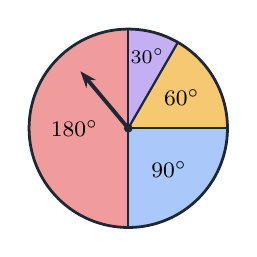
\begin{tikzpicture}[scale=1.05]
\fill[AnsRed!45] (0,0)--(90:1.2) arc (90:270:1.2)--cycle;
\fill[tmBlue!45] (0,0)--(270:1.2) arc (270:360:1.2)--cycle;
\fill[StarGold!70] (0,0)--(0:1.2) arc (0:60:1.2)--cycle;
\fill[tmPurple!45] (0,0)--(60:1.2) arc (60:90:1.2)--cycle;
\draw[Ink,line width=1pt] (0,0) circle (1.2);
\foreach \a in {90,270,0,60}{\draw[Ink,line width=0.8pt] (0,0)--(\a:1.2);}
\node[font=\footnotesize] at (180:0.65){$180^\circ$};
\node[font=\footnotesize] at (315:0.7){$90^\circ$};
\node[font=\footnotesize] at (30:0.75){$60^\circ$};
\node[font=\scriptsize] at (75:0.9){$30^\circ$};
\draw[-{Stealth[length=6pt]},line width=1.4pt,Ink] (0,0)--(130:0.9);\fill[Ink] (0,0) circle (1.5pt);
\end{tikzpicture}
\end{minipage}
\end{probbox}
\probsol{
\textbf{Phân tích đề.} Các ô có kích thước \emph{khác nhau}, nên bốn ô \emph{không} đồng khả năng. Ta không thể dùng ``$1$ ô trên $4$ ô''. Thay vào đó, khả năng kim dừng ở một ô tỉ lệ với độ lớn của ô, tức là với góc ở tâm của ô.
\begin{recallbox}Với bánh xe có các ô không bằng nhau: $P(\text{ô})=\dfrac{\text{góc ở tâm của ô}}{360^\circ}$. Cả vòng tròn có góc $360^\circ$.\end{recallbox}
\step{1}{Kiểm tra số liệu}
$180^\circ+90^\circ+60^\circ+30^\circ=360^\circ$ -- đúng bằng một vòng tròn \checkmark.
\step{2}{Câu a}
$P(\text{xanh})=\dfrac{90}{360}=\dfrac14$.

\emph{Cách nghĩ khác:} ta có thể chia bánh xe thành $12$ ô nhỏ bằng nhau, mỗi ô $30^\circ$. Khi đó đỏ chiếm $6$ ô nhỏ, xanh $3$ ô, vàng $2$ ô, tím $1$ ô; $12$ ô nhỏ này đồng khả năng. $P(\text{xanh})=\dfrac{3}{12}=\dfrac14$ \checkmark.
\step{3}{Câu b}
Ô vàng và ô tím không chồng lên nhau, nên góc tổng là $60^\circ+30^\circ=90^\circ$.
\[P(\text{vàng hoặc tím})=\frac{90}{360}=\frac14\quad\Big(\text{hoặc }\frac{2+1}{12}=\frac{3}{12}=\frac14\Big).\]
\step{4}{Câu c}
Leo nói \textbf{sai}. Công thức ``thuận lợi chia tất cả'' chỉ dùng được khi các kết quả \emph{đồng khả năng}. Ở đây bốn màu không đồng khả năng: ô đỏ chiếm nửa bánh xe nên $P(\text{đỏ})=\dfrac{180}{360}=\dfrac12$, còn $P(\text{tím})=\dfrac{30}{360}=\dfrac{1}{12}$ -- khác xa nhau.
\verify{$P(\text{đỏ})+P(\text{xanh})+P(\text{vàng})+P(\text{tím})=\dfrac{6}{12}+\dfrac{3}{12}+\dfrac{2}{12}+\dfrac{1}{12}=1$ \checkmark.}
\begin{parentbox}Có thể cắt một đĩa giấy thành $12$ ``miếng bánh'' bằng nhau rồi tô màu như đề bài. Trẻ đếm số miếng của mỗi màu sẽ hiểu ngay vì sao ô to thì xác suất lớn.\end{parentbox}
\ans{a) $\dfrac14$;\quad b) $\dfrac14$;\quad c) Sai, vì các ô không bằng nhau (ví dụ $P(\text{đỏ})=\dfrac12$, $P(\text{tím})=\dfrac1{12}$).}
}

% ---------------------------------------------------------------- Bài 33
\begin{probbox}{33}{\relax}
Căng tin trường có thực đơn bữa trưa: món chính chọn một trong $3$ món (cơm gà, mì Ý, pizza); đồ uống chọn một trong $2$ loại (nước táo, nước cam); tráng miệng chọn một trong $2$ món (kem, sữa chua). Mỗi suất ăn gồm một món chính, một đồ uống và một món tráng miệng.
\begin{enumerate}[label=\alph*),leftmargin=1.5em,itemsep=0pt,topsep=2pt]
\item Có bao nhiêu suất ăn khác nhau?
\item Bạn Mia được phát ngẫu nhiên một suất ăn. Tính xác suất suất ăn đó có mì Ý.
\item Tính xác suất suất ăn của Mia có cả mì Ý và nước cam.
\end{enumerate}
\end{probbox}
\probsol{
\textbf{Phân tích đề.} Mỗi suất ăn được tạo bởi ba bước chọn liên tiếp: món chính, đồ uống, tráng miệng. Được ``phát ngẫu nhiên'' nghĩa là mọi suất ăn khác nhau đều đồng khả năng.
\step{1}{Câu a -- quy tắc nhân}
\begin{recallbox}Quy tắc nhân: một việc gồm nhiều bước, bước 1 có $m$ cách, bước 2 có $n$ cách, bước 3 có $p$ cách thì có $m\times n\times p$ cách.\end{recallbox}
Số suất ăn: $3\times2\times2=12$.
\begin{center}\begin{tikzpicture}[grow'=right,level distance=2.6cm,font=\sffamily\footnotesize,
  every node/.style={draw=tmBlue,fill=tmBlue!8,rounded corners=2pt,inner sep=2pt},
  level 1/.style={sibling distance=2.4cm},level 2/.style={sibling distance=1.2cm},level 3/.style={sibling distance=0.6cm},
  edge from parent/.style={draw=Ink!60}]
\node[fill=Ink!10,draw=Ink]{Suất}
  child{node{cơm gà} child{node{nước táo} child{node{kem}} child{node{sữa chua}}} child{node{nước cam} child{node{kem}} child{node{sữa chua}}}}
  child{node[fill=tmOrange!25,draw=tmOrange]{mì Ý} child{node{nước táo} child{node{kem}} child{node{sữa chua}}} child{node[fill=tmOrange!25,draw=tmOrange]{nước cam} child{node[fill=tmOrange!25,draw=tmOrange]{kem}} child{node[fill=tmOrange!25,draw=tmOrange]{sữa chua}}}}
  child{node{pizza} child{node{nước táo} child{node{kem}} child{node{sữa chua}}} child{node{nước cam} child{node{kem}} child{node{sữa chua}}}};
\end{tikzpicture}\end{center}
Sơ đồ cây có $3$ nhánh lớn, mỗi nhánh lớn tỏa $2$ nhánh, mỗi nhánh đó lại tỏa $2$ nhánh: $12$ ngọn, đúng $12$ suất ăn.
\step{2}{Câu b}
Các suất có mì Ý: món chính cố định là mì Ý, đồ uống $2$ cách, tráng miệng $2$ cách: $1\times2\times2=4$ suất (nhánh giữa của sơ đồ cây).
$P(\text{có mì Ý})=\dfrac{4}{12}=\dfrac13$.
\begin{tipbox}Cũng có thể nghĩ nhanh: món chính được chọn ngẫu nhiên trong $3$ món, mỗi món xuất hiện trong số suất ăn như nhau, nên $P(\text{mì Ý})=\dfrac13$. Đồ uống và tráng miệng không ảnh hưởng.\end{tipbox}
\step{3}{Câu c}
Món chính là mì Ý, đồ uống là nước cam, chỉ còn chọn tráng miệng: $1\times1\times2=2$ suất (tô cam trên sơ đồ).
$P(\text{mì Ý và nước cam})=\dfrac{2}{12}=\dfrac16$.
\verify{Liệt kê: (mì Ý, nước cam, kem) và (mì Ý, nước cam, sữa chua) -- đúng $2$ suất \checkmark.}
\ans{a) $12$ suất;\quad b) $\dfrac13$;\quad c) $\dfrac16$.}
}

% ---------------------------------------------------------------- Bài 34
\begin{probbox}{34}{\relax}
Một hội trường có $20$ hàng ghế. Hàng thứ nhất có $12$ ghế, và mỗi hàng phía sau có nhiều hơn hàng ngay trước nó $2$ ghế.
\begin{enumerate}[label=\alph*),leftmargin=1.5em,itemsep=0pt,topsep=2pt]
\item Hàng thứ $20$ có bao nhiêu ghế?
\item Hàng thứ mấy có đúng $30$ ghế?
\item Hội trường có tất cả bao nhiêu ghế?
\end{enumerate}
\end{probbox}
\probsol{
\textbf{Phân tích đề.} Số ghế các hàng là $12;14;16;\dots$ -- một \emph{dãy cách đều} với khoảng cách $d=2$. Ta cần: số hạng thứ $20$, vị trí của số $30$ và tổng của $20$ số hạng.
\step{1}{Câu a -- tìm quy luật}
\begin{center}
\begin{tabular}{|c|c|c|c|c|c|}\hline
Hàng & $1$ & $2$ & $3$ & $4$ & $k$\\ \hline
Số ghế & $12$ & $12+2$ & $12+2\times2$ & $12+3\times2$ & $12+(k-1)\times2$\\ \hline
\end{tabular}
\end{center}
Từ hàng $1$ đến hàng $k$ có $k-1$ ``bước nhảy'', mỗi bước thêm $2$ ghế. Hàng $20$: $12+19\times2=12+38=50$ ghế.
\begin{warnbox}Không phải $12+20\times2=52$: từ hàng $1$ đến hàng $20$ chỉ có $19$ lần tăng (lỗi ``lệch một'').\end{warnbox}
\step{2}{Câu b}
Cần $12+(k-1)\times2=30$, tức $(k-1)\times2=18$, $k-1=9$, $k=10$. Hàng thứ $10$ có $30$ ghế.
\step{3}{Câu c -- tổng dãy cách đều}
\begin{recallbox}Tổng dãy cách đều $=\dfrac{(\text{số đầu}+\text{số cuối})\times\text{số số hạng}}{2}$ (cách ghép cặp của Gauss).\end{recallbox}
Tổng số ghế: $\dfrac{(12+50)\times20}{2}=\dfrac{62\times20}{2}=620$ ghế.
\begin{proofbox}Ghép hàng $1$ với hàng $20$: $12+50=62$; hàng $2$ với hàng $19$: $14+48=62$; \ldots; hàng $10$ với hàng $11$: $30+32=62$. Có $10$ cặp, mỗi cặp $62$ ghế, nên tổng là $10\times62=620$.\end{proofbox}
\verify{Cách khác: nếu mọi hàng đều có $12$ ghế thì có $20\times12=240$ ghế; phần ``thêm'' là $0+2+4+\dots+38=2\times(0+1+\dots+19)=2\times190=380$; tổng $240+380=620$ \checkmark.}
\ans{a) $50$ ghế;\quad b) hàng thứ $10$;\quad c) $620$ ghế.}
}

% ---------------------------------------------------------------- Bài 35
\begin{probbox}{35}{\stars{1}}
Một hộp chỉ chứa bi đỏ và bi xanh. Lấy ngẫu nhiên một viên thì xác suất được bi đỏ là $\dfrac35$. Nếu bỏ thêm vào hộp $5$ viên bi xanh thì xác suất lấy được bi đỏ chỉ còn $\dfrac12$. Hỏi lúc đầu trong hộp có bao nhiêu bi đỏ, bao nhiêu bi xanh?
\end{probbox}
\probsol{
\textbf{Phân tích đề.} Ta chưa biết số bi, chỉ biết hai xác suất (hai tỉ số). Ta gọi ẩn cho số bi đỏ và số bi xanh lúc đầu, dịch mỗi điều kiện thành một phương trình, rồi giải hệ hai phương trình. Lưu ý: thêm bi xanh thì số bi đỏ \emph{không đổi}, còn tổng số bi tăng thêm $5$.
\step{1}{Gọi ẩn}
Gọi $x$ là số bi đỏ và $y$ là số bi xanh lúc đầu ($x$, $y$ là số tự nhiên khác $0$). Lúc đầu hộp có $x+y$ viên bi.
\step{2}{Dịch điều kiện thứ nhất thành phương trình}
$P(\text{đỏ})=\dfrac{x}{x+y}=\dfrac35$. Nhân chéo: $5x=3(x+y)$, tức $5x=3x+3y$, hay
\[2x=3y.\qquad(1)\]
\begin{recallbox}$\dfrac ab=\dfrac cd$ (với $b$, $d$ khác $0$) khi và chỉ khi $a\times d=b\times c$.\end{recallbox}
\step{3}{Dịch điều kiện thứ hai thành phương trình}
Sau khi thêm $5$ bi xanh: vẫn có $x$ bi đỏ, tổng số bi là $x+y+5$. Ta có $\dfrac{x}{x+y+5}=\dfrac12$. Nhân chéo: $2x=x+y+5$, hay
\[x=y+5.\qquad(2)\]
(Nghĩa là: sau khi thêm, số bi đỏ \emph{bằng} số bi xanh.)
\step{4}{Giải hệ bằng phương pháp thế}
Thay $x=y+5$ từ (2) vào (1):
\[2(y+5)=3y\ \Rightarrow\ 2y+10=3y\ \Rightarrow\ 3y-2y=10\ \Rightarrow\ y=10.\]
Khi đó $x=y+5=10+5=15$.
\begin{tipbox}\emph{Cách dùng tỉ lệ:} từ (1), $\dfrac x3=\dfrac y2$; đặt $\dfrac x3=\dfrac y2=k$ thì $x=3k$, $y=2k$. Thay vào (2): $3k=2k+5$, nên $k=5$, $x=15$, $y=10$.\end{tipbox}
\verify{Lúc đầu: $15$ đỏ, $10$ xanh, $P(\text{đỏ})=\dfrac{15}{25}=\dfrac35$ \checkmark. Thêm $5$ xanh: $15$ đỏ, $15$ xanh, $P(\text{đỏ})=\dfrac{15}{30}=\dfrac12$ \checkmark.}
\begin{warnbox}Đừng giải bằng cách ``trừ xác suất'': $\dfrac35-\dfrac12=\dfrac1{10}$ không cho biết gì trực tiếp về số bi. Xác suất là \emph{tỉ số}, phải quay về số lượng cụ thể.\end{warnbox}
\ans{Lúc đầu có $15$ bi đỏ và $10$ bi xanh.}
}

% ---------------------------------------------------------------- Bài 36

\begin{probbox}{36}{\stars{1}}
Nhắc lại: số đối xứng là số đọc xuôi hay đọc ngược đều như nhau (ví dụ $3443$, $7007$).
\begin{enumerate}[label=\alph*),leftmargin=1.5em,itemsep=0pt,topsep=2pt]
\item Có bao nhiêu số đối xứng có bốn chữ số?
\item Trong đó có bao nhiêu số chẵn?
\item Chọn ngẫu nhiên một số đối xứng có bốn chữ số. Tính xác suất số đó là số chẵn.
\item Chứng tỏ rằng mọi số đối xứng có bốn chữ số đều chia hết cho $11$.
\end{enumerate}
\end{probbox}
\probsol{
\textbf{Phân tích đề.} Số có bốn chữ số $\overline{abcd}$ là số đối xứng khi đọc ngược $\overline{dcba}$ vẫn là nó: $d=a$ và $c=b$. Vậy số đối xứng có bốn chữ số có dạng $\overline{abba}$, và chỉ có \emph{hai} chữ số được chọn tự do: $a$ và $b$.
\step{1}{Câu a}
\begin{recallbox}Quy tắc nhân; chữ số đầu tiên của một số không được là $0$.\end{recallbox}
\begin{center}\begin{tabular}{|l|c|c|c|c|}\hline
Chữ số & thứ nhất ($a$) & thứ hai ($b$) & thứ ba & thứ tư\\ \hline
Điều kiện & từ $1$ đến $9$ & từ $0$ đến $9$ & bằng $b$ & bằng $a$\\ \hline
Số cách chọn & $9$ & $10$ & $1$ & $1$\\ \hline
\end{tabular}\end{center}
$a$: $9$ cách ($1$ đến $9$); $b$: $10$ cách; hai chữ số sau bị ép bằng $b$ và $a$. Có $9\times10=90$ số.
\step{2}{Câu b}
Số chẵn khi chữ số hàng đơn vị chẵn. Chữ số hàng đơn vị chính là $a$, nên $a$ phải chẵn \emph{và} khác $0$: $a\in\{2;4;6;8\}$ -- $4$ cách. $b$ vẫn có $10$ cách. Có $4\times10=40$ số chẵn.
\begin{warnbox}Chữ số $0$ là chữ số chẵn, nhưng $a=0$ bị loại vì $a$ còn là chữ số đầu tiên. Vì vậy chỉ có $4$ chứ không phải $5$ lựa chọn cho $a$.\end{warnbox}
\step{3}{Câu c}
$P(\text{chẵn})=\dfrac{40}{90}=\dfrac49$.
\step{4}{Câu d -- chứng minh}
\begin{proofbox}Viết số $\overline{abba}$ theo giá trị các hàng:
$\overline{abba}=1000a+100b+10b+a=1001a+110b$.
Mà $1001=11\times91$ và $110=11\times10$, nên
$\overline{abba}=11\times91\times a+11\times10\times b=11\times(91a+10b)$,
là một số chia hết cho $11$.\end{proofbox}
\verify{Ví dụ: $3443=11\times313$; $7007=11\times637$; $1221=11\times111$ \checkmark. Kiểm tra đếm: các số đối xứng bắt đầu bằng $1$ là $1001;1111;\dots;1991$ -- đúng $10$ số; chín chữ số đầu cho $90$ số \checkmark.}
\ans{a) $90$;\quad b) $40$;\quad c) $\dfrac49$;\quad d) $\overline{abba}=11\times(91a+10b)$.}
}

% ---------------------------------------------------------------- Bài 37

\begin{probbox}{37}{\stars{1}}
Từ bốn chữ số $0;1;2;3$, lập các số có bốn chữ số đôi một khác nhau (mỗi chữ số dùng đúng một lần).
\begin{enumerate}[label=\alph*),leftmargin=1.5em,itemsep=0pt,topsep=2pt]
\item Lập được bao nhiêu số như vậy?
\item Có bao nhiêu số chẵn trong các số đó?
\item Chọn ngẫu nhiên một số trong các số ở câu a). Tính xác suất số đó là số chẵn.
\end{enumerate}
\end{probbox}
\probsol{
\textbf{Phân tích đề.} Mỗi số là một cách xếp bốn chữ số $0;1;2;3$ vào bốn hàng (nghìn, trăm, chục, đơn vị), với điều kiện chữ số hàng nghìn khác $0$.
\step{1}{Câu a -- chọn vị trí có điều kiện trước}
\begin{recallbox}Quy tắc nhân. Vị trí nào có điều kiện thì chọn trước.\end{recallbox}
\begin{center}\begin{tabular}{|l|c|c|c|c|}\hline
Hàng & nghìn & trăm & chục & đơn vị\\ \hline
Điều kiện & khác $0$ & $3$ chữ số còn lại & $2$ chữ số còn lại & chữ số cuối\\ \hline
Số cách chọn & $3$ & $3$ & $2$ & $1$\\ \hline
\end{tabular}\end{center}
Hàng nghìn: $3$ cách ($1$, $2$ hoặc $3$). Hàng trăm: còn $3$ chữ số (bây giờ được dùng $0$): $3$ cách. Hàng chục: $2$ cách. Hàng đơn vị: $1$ cách. Có $3\times3\times2\times1=18$ số.
\begin{warnbox}Nếu quên điều kiện ``hàng nghìn khác $0$'' sẽ được $4\times3\times2\times1=24$ -- trong đó có $6$ ``số'' bắt đầu bằng $0$ như $0123$, thực chất chỉ là số có ba chữ số.\end{warnbox}
\step{2}{Câu b -- chia trường hợp theo chữ số hàng đơn vị}
Số chẵn thì hàng đơn vị là $0$ hoặc $2$. Hai trường hợp này khác nhau ở chỗ: chữ số $0$ có ảnh hưởng đến hàng nghìn.
\begin{itemize}[leftmargin=1.2em,itemsep=1pt,topsep=1pt]
\item \textbf{Trường hợp 1: hàng đơn vị là $0$.} Ba chữ số $1;2;3$ xếp tự do vào ba hàng còn lại (không còn lo chữ số $0$ ở đầu): $3\times2\times1=6$ số.
\item \textbf{Trường hợp 2: hàng đơn vị là $2$.} Còn $0;1;3$. Hàng nghìn khác $0$: $2$ cách ($1$ hoặc $3$); hàng trăm: $2$ cách; hàng chục: $1$ cách. Có $2\times2\times1=4$ số.
\end{itemize}
\begin{recallbox}Quy tắc cộng: các trường hợp tách rời nhau thì cộng số cách của từng trường hợp.\end{recallbox}
Số các số chẵn: $6+4=10$.
\step{3}{Câu c}
$P(\text{chẵn})=\dfrac{10}{18}=\dfrac59$.
\verify{Liệt kê các số chẵn. TH1: $1230;1320;2130;2310;3120;3210$ ($6$ số). TH2: $1032;1302;3012;3102$ ($4$ số). Tổng $10$ \checkmark. Số lẻ (tận cùng $1$ hoặc $3$): mỗi trường hợp giống TH2, có $4$ số, tổng $8$; và $10+8=18$ \checkmark.}
\ans{a) $18$ số;\quad b) $10$ số chẵn;\quad c) $\dfrac59$.}
}

% ---------------------------------------------------------------- Bài 38
\begin{probbox}{38}{\stars{1}}
\begin{minipage}[t]{0.62\linewidth}\vspace{0pt}
Hình bên là một lưới hình chữ nhật gồm $2$ hàng, $3$ cột ô vuông.
\begin{enumerate}[label=\alph*),leftmargin=1.5em,itemsep=0pt,topsep=2pt]
\item Trong hình có tất cả bao nhiêu hình chữ nhật (kể cả hình vuông)?
\item Có bao nhiêu hình vuông?
\item Chọn ngẫu nhiên một hình chữ nhật trong số đó. Tính xác suất nó là hình vuông.
\end{enumerate}
\end{minipage}\hfill
\begin{minipage}[t]{0.34\linewidth}\vspace{0pt}
\centering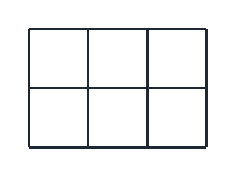
\begin{tikzpicture}[scale=0.75]
\foreach \x in {0,1,2,3}{\draw[Ink,line width=1pt] (\x,0)--(\x,2);}
\foreach \y in {0,1,2}{\draw[Ink,line width=1pt] (0,\y)--(3,\y);}
\end{tikzpicture}
\end{minipage}
\end{probbox}
\probsol{
\textbf{Phân tích đề.} Đây là một lưới kẻ suốt, nên dùng được mẹo ``chọn hai đường''. Ta cũng sẽ đếm theo kích thước để kiểm tra lại.
\step{1}{Câu a -- chọn hai đường ngang và hai đường dọc}
\begin{recallbox}Một hình chữ nhật trong lưới được xác định bởi $2$ đường ngang và $2$ đường dọc. Số cách chọn $2$ đường trong $n$ đường là $\dfrac{n\times(n-1)}{2}$.\end{recallbox}
Lưới có $3$ đường ngang và $4$ đường dọc.
\begin{itemize}[leftmargin=1.2em,itemsep=0pt,topsep=1pt]
\item Chọn $2$ đường ngang: $\dfrac{3\times2}{2}=3$ cách.
\item Chọn $2$ đường dọc: $\dfrac{4\times3}{2}=6$ cách.
\end{itemize}
Theo quy tắc nhân: $3\times6=18$ hình chữ nhật.
\step{2}{Kiểm tra bằng bảng kích thước}
Kí hiệu ``cao $\times$ rộng'' (theo số ô). Một hình rộng $w$ ô có $4-w$ vị trí theo chiều ngang; cao $h$ ô có $3-h$ vị trí theo chiều dọc.
\begin{center}
\begin{tabular}{|c|c|c|c|c|c|c|c|}\hline
Kích thước & $1\times1$ & $1\times2$ & $1\times3$ & $2\times1$ & $2\times2$ & $2\times3$ & Tổng\\ \hline
Số hình & $2\times3=6$ & $2\times2=4$ & $2\times1=2$ & $1\times3=3$ & $1\times2=2$ & $1\times1=1$ & $18$\\ \hline
\end{tabular}
\end{center}
Hai cách cho cùng kết quả $18$ \checkmark.
\step{3}{Câu b}
Hình vuông là các hình $1\times1$ và $2\times2$: $6+2=8$ hình vuông.
\begin{warnbox}Không có hình vuông $3\times3$ vì lưới chỉ cao $2$ ô. Và đừng quên hai hình vuông $2\times2$ (bên trái và bên phải, chồng lên nhau ở cột giữa).\end{warnbox}
\step{4}{Câu c}
$P(\text{hình vuông})=\dfrac{8}{18}=\dfrac49$.
\ans{a) $18$;\quad b) $8$;\quad c) $\dfrac49$.}
}

% ---------------------------------------------------------------- Bài 39
\begin{probbox}{39}{\stars{1}}
Bốn bạn Anna, Ben, Chloe và David được xếp ngẫu nhiên vào bốn chiếc ghế xếp thành một hàng ngang.
\begin{enumerate}[label=\alph*),leftmargin=1.5em,itemsep=0pt,topsep=2pt]
\item Có bao nhiêu cách xếp chỗ?
\item Tính xác suất Anna và Ben ngồi cạnh nhau.
\item Tính xác suất Anna và Ben ngồi ở hai đầu hàng.
\end{enumerate}
\end{probbox}
\probsol{
\textbf{Phân tích đề.} ``Xếp ngẫu nhiên'' nghĩa là mọi cách xếp đều đồng khả năng. Ta đếm tổng số cách xếp, rồi đếm số cách thuận lợi cho từng biến cố. Đánh số ghế $1;2;3;4$ từ trái sang phải.
\step{1}{Câu a}
\begin{recallbox}Xếp $n$ người vào $n$ ghế: $n\times(n-1)\times\dots\times2\times1$ cách (quy tắc nhân, mỗi ghế sau còn ít hơn một người để chọn).\end{recallbox}
Ghế $1$: $4$ cách chọn người; ghế $2$: $3$ cách; ghế $3$: $2$ cách; ghế $4$: $1$ cách. Có $4\times3\times2\times1=24$ cách.
\step{2}{Câu b -- xem Anna và Ben là một ``khối''}
Ghép Anna và Ben thành một ``khối'' chiếm $2$ ghế liền nhau. Bảng dưới đây cho thấy khối chỉ có $3$ vị trí:
\begin{center}\begin{tabular}{|c|c|c|c|c|}\hline
 & Ghế $1$ & Ghế $2$ & Ghế $3$ & Ghế $4$\\ \hline
Vị trí 1 & \multicolumn{2}{c|}{\cellcolor{tmOrange!20}Anna và Ben} & & \\ \hline
Vị trí 2 & & \multicolumn{2}{c|}{\cellcolor{tmOrange!20}Anna và Ben} & \\ \hline
Vị trí 3 & & & \multicolumn{2}{c|}{\cellcolor{tmOrange!20}Anna và Ben}\\ \hline
\end{tabular}\end{center}
\begin{itemize}[leftmargin=1.2em,itemsep=1pt,topsep=1pt]
\item Vị trí của khối (Anna, Ben): chiếm ghế $1$--$2$, $2$--$3$ hoặc $3$--$4$: $3$ cách.
\item Trong khối, Anna bên trái hoặc Ben bên trái: $2$ cách.
\item Chloe và David xếp vào $2$ ghế còn lại: $2\times1=2$ cách.
\end{itemize}
Số cách thuận lợi: $3\times2\times2=12$. Vậy $P(\text{cạnh nhau})=\dfrac{12}{24}=\dfrac12$.
\begin{warnbox}Đừng quên nhân $2$ cho việc đổi chỗ Anna và Ben bên trong khối: ``Anna--Ben'' và ``Ben--Anna'' là hai cách xếp khác nhau.\end{warnbox}
\step{3}{Câu c}
Anna và Ben ở ghế $1$ và ghế $4$: Anna ở ghế $1$, Ben ở ghế $4$ hoặc ngược lại -- $2$ cách. Chloe và David vào ghế $2$, $3$: $2$ cách. Số cách thuận lợi: $2\times2=4$.
$P(\text{hai đầu})=\dfrac{4}{24}=\dfrac16$.
\verify{Câu b, đếm theo cách khác: Anna ngồi ở đầu hàng (ghế $1$ hoặc $4$, $2$ khả năng) thì chỉ có $1$ ghế cạnh Anna; Anna ngồi ở giữa (ghế $2$ hoặc $3$) thì có $2$ ghế cạnh Anna. Số cặp ghế (Anna, Ben) cạnh nhau: $2\times1+2\times2=6$; nhân với $2$ cách xếp Chloe, David: $12$ \checkmark.}
\begin{parentbox}Với bài $4$ người, có thể cho trẻ dùng $4$ tấm thẻ ghi tên và thật sự xếp hết $24$ cách theo thứ tự (bắt đầu bằng Anna, rồi bắt đầu bằng Ben\ldots). Liệt kê một lần giúp trẻ tin vào quy tắc nhân.\end{parentbox}
\ans{a) $24$ cách;\quad b) $\dfrac12$;\quad c) $\dfrac16$.}
}

% ---------------------------------------------------------------- Bài 40
\begin{probbox}{40}{\stars{2}}
Một hộp có $4$ viên bi đỏ và $6$ viên bi xanh có cùng kích thước. Bạn Grace lấy ngẫu nhiên một viên bi, \emph{không trả lại}, rồi lấy ngẫu nhiên tiếp viên thứ hai.
\begin{enumerate}[label=\alph*),leftmargin=1.5em,itemsep=0pt,topsep=2pt]
\item Tính xác suất cả hai viên đều là bi đỏ.
\item Tính xác suất hai viên bi cùng màu.
\item Tính xác suất hai viên bi khác màu.
\end{enumerate}
\end{probbox}
\probsol{
\textbf{Phân tích đề.} Grace lấy \emph{lần lượt} hai viên và không trả lại. Hãy tưởng tượng các viên bi được đánh số $1$ đến $10$ (bi $1$--$4$ đỏ, bi $5$--$10$ xanh). Mỗi \emph{cặp có thứ tự} (viên thứ nhất, viên thứ hai) là một kết quả, và các kết quả này đồng khả năng.
\step{1}{Đếm tất cả các kết quả}
\begin{recallbox}Quy tắc nhân: lần $1$ có $10$ cách; với mỗi cách đó, lần $2$ còn $9$ viên nên có $9$ cách.\end{recallbox}
Số kết quả: $10\times9=90$ cặp có thứ tự.
\step{2}{Câu a -- cả hai đỏ}
Lần $1$ lấy bi đỏ: $4$ cách. Khi đó còn $3$ bi đỏ, lần $2$ lấy bi đỏ: $3$ cách. Số kết quả thuận lợi: $4\times3=12$.
$P(\text{đỏ, đỏ})=\dfrac{12}{90}=\dfrac{2}{15}$.
\step{3}{Sơ đồ cây có ghi số cách}
\begin{center}\begin{tikzpicture}[grow'=right,level distance=3.1cm,font=\sffamily\footnotesize,
  every node/.style={draw=Ink!60,rounded corners=2pt,inner sep=2.5pt,fill=white},
  level 1/.style={sibling distance=2.2cm},level 2/.style={sibling distance=1.1cm},
  edge from parent/.style={draw=Ink!60}]
\node[fill=Ink!10]{Bắt đầu}
  child{node[fill=AnsRed!15,draw=AnsRed]{Đỏ: $4$ cách}
     child{node[fill=AnsRed!15,draw=AnsRed]{Đỏ: $3$ cách $\Rightarrow 4\times3=12$}}
     child{node[fill=tmBlue!15,draw=tmBlue]{Xanh: $6$ cách $\Rightarrow 4\times6=24$}}}
  child{node[fill=tmBlue!15,draw=tmBlue]{Xanh: $6$ cách}
     child{node[fill=AnsRed!15,draw=AnsRed]{Đỏ: $4$ cách $\Rightarrow 6\times4=24$}}
     child{node[fill=tmBlue!15,draw=tmBlue]{Xanh: $5$ cách $\Rightarrow 6\times5=30$}}};
\end{tikzpicture}\end{center}
Kiểm tra: $12+24+24+30=90$ \checkmark{} -- bốn nhánh phủ hết mọi kết quả.
\step{4}{Câu b -- cùng màu}
Cùng màu gồm hai trường hợp tách rời: (đỏ, đỏ) có $12$ kết quả và (xanh, xanh) có $30$ kết quả.
\begin{recallbox}Quy tắc cộng cho các trường hợp không chồng lên nhau.\end{recallbox}
Số kết quả thuận lợi: $12+30=42$. $P(\text{cùng màu})=\dfrac{42}{90}=\dfrac{7}{15}$.
\step{5}{Câu c -- biến cố đối}
``Khác màu'' là biến cố đối của ``cùng màu'': $P(\text{khác màu})=1-\dfrac{7}{15}=\dfrac{8}{15}$.
\verify{Đếm trực tiếp: (đỏ, xanh) $24$ và (xanh, đỏ) $24$, tổng $48$; $\dfrac{48}{90}=\dfrac{8}{15}$ \checkmark.}
\begin{warnbox}Lỗi hay gặp nhất: coi như lần hai vẫn còn đủ $10$ viên, tính $\dfrac{4}{10}\times\dfrac{4}{10}$ hoặc đếm $4\times4$ cặp đỏ. Vì \emph{không trả lại}, lần hai chỉ còn $9$ viên và chỉ còn $3$ viên đỏ.\end{warnbox}
\begin{tipbox}Có thể đếm không theo thứ tự: số cách chọn $2$ viên trong $10$ viên là $\dfrac{10\times9}{2}=45$, số cách chọn $2$ viên đỏ trong $4$ viên là $\dfrac{4\times3}{2}=6$, nên $P(\text{đỏ, đỏ})=\dfrac{6}{45}=\dfrac{2}{15}$ -- cùng kết quả. Điều quan trọng là tử số và mẫu số phải đếm \emph{cùng một kiểu} (cùng có thứ tự hoặc cùng không thứ tự).\end{tipbox}
\ans{a) $\dfrac{2}{15}$;\quad b) $\dfrac{7}{15}$;\quad c) $\dfrac{8}{15}$.}
}

% ---------------- part d ----------------
% ================= Topic 3 (VI) -- part d: problems 41--50 (nâng cao) =================
\begin{probbox}{41}{\stars{1}}
Trên một lưới điểm vuông, bạn Ruby đứng ở điểm $A$. Ruby tung một đồng xu cân đối $6$ lần; mỗi lần ra mặt sấp thì Ruby đi
\emph{lên} một điểm, ra mặt ngửa thì Ruby đi \emph{sang phải} một điểm (như bài 16). Các điểm $M$, $N$, $B$ được đánh dấu
trên hình.
\begin{figC}\begin{scope}[scale=0.85]
  \foreach \x in {0,...,3}{\foreach \y in {0,...,3}{\fill[Navy] (\x,\y) circle (2.4pt);}}
  \fill[tmOrange] (0,0) circle (3.4pt);\node[below left] at (0,0) {$A$};
  \fill[tmGreen!80!black] (1,1) circle (3.4pt);\node[above left] at (1,1) {$M$};
  \fill[AnsRed] (2,1) circle (3.4pt);\node[below right] at (2,1) {$N$};
  \fill[tmPurple] (3,3) circle (3.4pt);\node[above right] at (3,3) {$B$};
\end{scope}\end{figC}
\begin{enumerate}[label=\alph*),leftmargin=1.6em,itemsep=1pt,topsep=2pt]
\item Tính xác suất để sau $6$ lần tung, Ruby dừng ở điểm $B$.
\item Tính xác suất để Ruby đi qua điểm $M$ \emph{và} dừng ở $B$.
\item Tính xác suất để Ruby dừng ở $B$ mà \emph{không} đi qua điểm $N$.
\end{enumerate}
\end{probbox}
\needspace{8\baselineskip}
\probsol{
\textbf{Phân tích đề.} Mỗi dãy $6$ lần tung là một dãy gồm $6$ kí hiệu $\uparrow$ (lên) hoặc $\rightarrow$ (sang phải).
Có $2^6=2\times2\times2\times2\times2\times2=64$ dãy, đồng khả năng. Mỗi dãy là một \emph{đường đi} trên lưới.
Ta đánh dấu vị trí bằng cặp (số bước sang phải, số bước lên): $A=(0,0)$, $M=(1,1)$, $N=(2,1)$, $B=(3,3)$.

\step{1}{Đếm số đường đi từ $A$ tới mỗi điểm (câu a)}
\begin{recallbox}Một điểm chỉ có thể tới được từ điểm ngay bên trái hoặc ngay bên dưới nó. Vì vậy:
số đường tới một điểm $=$ số đường tới điểm bên trái $+$ số đường tới điểm bên dưới (quy tắc cộng).\end{recallbox}
Ghi số đường đi vào từng điểm, bắt đầu từ $A$ (ghi $1$); hàng dưới cùng và cột trái cùng đều là $1$:
\begin{figC}\begin{scope}[scale=0.85]
  \foreach \x/\y/\n in {0/0/1,1/0/1,2/0/1,3/0/1,0/1/1,1/1/2,2/1/3,3/1/4,0/2/1,1/2/3,2/2/6,3/2/10,0/3/1,1/3/4,2/3/10,3/3/20}{
    \fill[tmBlue!12] (\x,\y) circle (9pt);\node[font=\small\bfseries,text=Navy] at (\x,\y) {\n};}
  \draw[tmPurple,thick] (3,3) circle (10pt);\node[right=9pt,text=tmPurple] at (3,3) {$B$};
\end{scope}\end{figC}
Có $20$ đường đi từ $A$ tới $B$. (Cách khác: đi tới $B$ cần đúng $3$ bước lên trong $6$ bước; số cách chọn $3$ lượt
trong $6$ lượt là $\dfrac{6\times5\times4}{3\times2\times1}=20$.)
\[P(a)=\frac{20}{64}=\frac{5}{16}.\]

\step{2}{Câu b: đi qua $M$ rồi tới $B$ -- quy tắc nhân}
Một đường qua $M$ gồm hai chặng: chặng $A\to M$ ($1$ bước lên, $1$ bước phải) và chặng $M\to B$ ($2$ bước lên, $2$ bước phải).
Chặng $A\to M$ có $2$ cách ($\uparrow\rightarrow$ hoặc $\rightarrow\uparrow$); chặng $M\to B$ có $6$ cách (giống bài 16:
chọn $2$ lượt lên trong $4$ lượt). Mỗi cách đi chặng đầu ghép với mỗi cách đi chặng sau cho một đường khác nhau:
$2\times6=12$ đường.
\[P(b)=\frac{12}{64}=\frac{3}{16}.\]

\step{3}{Câu c: không đi qua $N$ -- dùng phần bù}
Số đường từ $A$ qua $N$ tới $B$: chặng $A\to N$ ($2$ bước phải, $1$ bước lên) có $3$ cách; chặng $N\to B$ ($1$ bước phải,
$2$ bước lên) có $3$ cách; tổng $3\times3=9$ đường. Vậy số đường từ $A$ tới $B$ \emph{không} qua $N$ là $20-9=11$.
\[P(c)=\frac{11}{64}.\]
\begin{proofbox}\emph{Kiểm tra bằng cách ``chặn'' điểm $N$.} Ghi lại số đường đi nhưng đặt số $0$ tại $N$ (coi như không được đi qua).
Hàng $1$: $1,\ 2,\ \mathbf{0},\ 0+1=1$. Hàng $2$: $1,\ 3,\ 3+0=3,\ 3+1=4$. Hàng $3$: $1,\ 4,\ 4+3=7,\ 7+4=11$.
Tại $B$ được $11$, khớp với phần bù.\end{proofbox}
\begin{warnbox}Câu b và c hỏi về xác suất trong \emph{toàn bộ} $64$ dãy tung, không phải trong $20$ đường tới $B$. Nếu chia cho $20$
là trả lời một câu hỏi khác (xác suất có điều kiện, chưa học).\end{warnbox}
\verify{Ở câu a, các điểm cuối có thể là $(6,0),(5,1),\dots,(0,6)$ với số đường $1,6,15,20,15,6,1$; tổng $=64$. Điểm $B=(3,3)$ ứng với số $20$.}
\ans{a) $\dfrac5{16}$;\quad b) $\dfrac3{16}$;\quad c) $\dfrac{11}{64}$}
}

\begin{probbox}{42}{\stars{2}}
Ta xếp các lưới ô vuông bằng que tăm như ở bài 17. Một lưới ``$m\times n$'' có $m$ hàng, mỗi hàng $n$ ô vuông.
\begin{enumerate}[label=\alph*),leftmargin=1.6em,itemsep=1pt,topsep=2pt]
\item Lập công thức tính số que tăm cần dùng cho lưới $m\times n$.
\item Một lưới hình vuông $k\times k$ dùng hết đúng $760$ que tăm. Tìm $k$.
\item Bạn Sam có đúng $2026$ que tăm và muốn xếp một lưới $m\times n$ (với $1\le m\le n$) dùng \emph{hết} số que này.
Tìm tất cả các lưới Sam có thể xếp.
\end{enumerate}
\end{probbox}
\probsol{
\textbf{Phân tích đề.} Giống bài 17, ta đếm riêng que nằm ngang và que thẳng đứng. Câu c dẫn tới một phương trình với hai ẩn
là số tự nhiên; mẹo ``nhân $2$ rồi cộng $1$'' giúp biến nó thành bài toán tìm ước.

\step{1}{Câu a: công thức}
Lưới $m\times n$ có $m+1$ đường kẻ ngang, mỗi đường $n$ que: $(m+1)\times n$ que nằm ngang. Có $n+1$ đường kẻ dọc, mỗi đường
$m$ que: $(n+1)\times m$ que thẳng đứng. Tổng:
\[T=(m+1)n+(n+1)m=mn+n+mn+m=2mn+m+n.\]
Thử lại với lưới $1\times10$: $2\times1\times10+1+10=31$. Đúng như bài 17.

\step{2}{Câu b: lưới vuông $k\times k$}
Thay $m=n=k$: $T=2k^2+2k=2k(k+1)$. Ta cần $2k(k+1)=760$, tức $k(k+1)=380$.
$k(k+1)$ là tích hai số tự nhiên liên tiếp. Vì $19\times20=380$, nên $k=19$. (Khi $k$ tăng thì $k(k+1)$ tăng, nên chỉ có một
giá trị: $18\times19=342<380<420=20\times21$.)

\step{3}{Câu c: lập phương trình}
Cần tìm các số tự nhiên $1\le m\le n$ với $2mn+m+n=2026$.
\begin{tipbox}Nhân hai vế với $2$ rồi cộng $1$: $4mn+2m+2n+1=4053$. Vế trái phân tích được thành tích:
$(2m+1)(2n+1)=4mn+2m+2n+1$ (nhân phân phối để kiểm tra). Vậy
\[(2m+1)(2n+1)=4053.\]\end{tipbox}

\step{4}{Phân tích $4053$ ra thừa số nguyên tố}
$4053$ có tổng chữ số $4+0+5+3=12$ chia hết cho $3$: $4053=3\times1351$. Tiếp theo $1351=7\times193$.
Số $193$ là số nguyên tố: nó không chia hết cho $2,3,5,7,11,13$, và $13\times13=169<193<196=14\times14$, nên không cần thử thêm.
\begin{recallbox}Để kiểm tra $N$ có là số nguyên tố không, chỉ cần thử chia cho các số nguyên tố $p$ với $p\times p\le N$.\end{recallbox}
Vậy $4053=3\times7\times193$. Các ước của $4053$ là: $1,\ 3,\ 7,\ 21,\ 193,\ 579,\ 1351,\ 4053$.

\step{5}{Tìm các cặp $(m,n)$}
Vì $m\ge1$ nên $2m+1\ge3$; vì $m\le n$ nên $2m+1\le2n+1$. Các cách viết $4053$ thành tích hai ước thỏa mãn:
\begin{center}\begin{tabular}{|c|c|c|c|c|}\hline
$2m+1$ & $2n+1$ & $m$ & $n$ & Thử lại $2mn+m+n$\\\hline
$3$ & $1351$ & $1$ & $675$ & $1350+1+675=2026$\\\hline
$7$ & $579$ & $3$ & $289$ & $1734+3+289=2026$\\\hline
$21$ & $193$ & $10$ & $96$ & $1920+10+96=2026$\\\hline
\end{tabular}\end{center}
(Cặp $1\times4053$ bị loại vì cho $m=0$.)
\begin{warnbox}Thử từng giá trị $m=1,2,3,\dots$ cũng làm được nhưng rất dài, dễ sót. Mẹo nhân $2$ cộng $1$ biến bài toán thành
``tìm ước'' và đảm bảo \emph{không bỏ sót} nghiệm nào.\end{warnbox}
\verify{Ở các giá trị $m$ khác, $2m+1$ không phải là ước của $4053$ nên $n$ không là số tự nhiên. Ví dụ $m=2$: $5(2n+1)=4053$ không
được vì $4053$ không chia hết cho $5$.}
\ans{a) $2mn+m+n$;\quad b) $k=19$;\quad c) ba lưới: $1\times675$, $3\times289$, $10\times96$}
}

\begin{probbox}{43}{\stars{1}}
Gieo cùng lúc ba con xúc xắc cân đối có màu đỏ, xanh và vàng (mỗi con ghi số từ $1$ đến $6$). Tính xác suất của các biến cố:
\begin{enumerate}[label=\alph*),leftmargin=1.6em,itemsep=1pt,topsep=2pt]
\item ba số xuất hiện đôi một khác nhau;
\item số trên con đỏ nhỏ hơn số trên con xanh, và số trên con xanh nhỏ hơn số trên con vàng;
\item có ít nhất một con xúc xắc ra số $6$;
\item số lớn nhất trong ba số xuất hiện bằng đúng $4$.
\end{enumerate}
\end{probbox}
\probsol{
\textbf{Phân tích đề.} Mỗi kết quả là bộ ba (đỏ, xanh, vàng). Theo quy tắc nhân có $6\times6\times6=216$ kết quả đồng khả năng.

\step{1}{Câu a: ba số khác nhau}
Con đỏ: $6$ cách; con xanh khác con đỏ: $5$ cách; con vàng khác hai con kia: $4$ cách. Có $6\times5\times4=120$ kết quả.
\[P(a)=\frac{120}{216}=\frac{5}{9}.\]

\step{2}{Câu b: đỏ $<$ xanh $<$ vàng -- dùng tính đối xứng}
Xét một bộ ba số khác nhau, chẳng hạn $\{2,3,5\}$. Có $3\times2\times1=6$ cách xếp ba số này cho ba con xúc xắc
($235$, $253$, $325$, $352$, $523$, $532$), và \emph{chỉ đúng một} cách là tăng dần ($2<3<5$).
Như vậy $120$ kết quả ở câu a chia thành các nhóm $6$, mỗi nhóm có $1$ kết quả thuận lợi: số kết quả thuận lợi là $120:6=20$.
\[P(b)=\frac{20}{216}=\frac{5}{54}.\]
\begin{recallbox}Số cách xếp $3$ vật khác nhau vào $3$ chỗ là $3\times2\times1=6$.\end{recallbox}

\step{3}{Câu c: ít nhất một số $6$ -- phần bù}
Biến cố đối là ``không con nào ra $6$'': mỗi con chỉ có $5$ kết quả ($1$ đến $5$), tổng $5\times5\times5=125$.
Vậy số kết quả có ít nhất một số $6$ là $216-125=91$.
\[P(c)=\frac{91}{216}.\]
\begin{warnbox}Không được tính ``mỗi con có xác suất $\frac16$ ra số $6$, ba con là $\frac36=\frac12$''. Cách cộng đó đếm trùng các kết quả
có hai hoặc ba số $6$ (như $(6,6,1)$ bị đếm hai lần).\end{warnbox}

\step{4}{Câu d: số lớn nhất bằng đúng $4$}
``Số lớn nhất $\le4$'' nghĩa là cả ba số đều thuộc $\{1,2,3,4\}$: $4\times4\times4=64$ kết quả.
``Số lớn nhất $\le3$'': $3\times3\times3=27$ kết quả. Số lớn nhất bằng đúng $4$ khi nó $\le4$ nhưng không $\le3$:
$64-27=37$ kết quả.
\[P(d)=\frac{37}{216}.\]
\begin{proofbox}Mọi kết quả có số lớn nhất $\le3$ đều nằm trong nhóm có số lớn nhất $\le4$. Bớt đi nhóm nhỏ còn lại đúng các kết
quả mà số lớn nhất không vượt quá $4$ nhưng vượt quá $3$, tức là bằng $4$.\end{proofbox}
\verify{Cách nghĩ của câu d áp dụng cho câu c: số lớn nhất bằng $6$ có $6^3-5^3=216-125=91$ kết quả, khớp. Tổng số kết quả theo
số lớn nhất $1,2,\dots,6$: $1+7+19+37+61+91=216$.}
\ans{a) $\dfrac59$;\quad b) $\dfrac5{54}$;\quad c) $\dfrac{91}{216}$;\quad d) $\dfrac{37}{216}$}
}

\begin{probbox}{44}{\stars{2}}
Người ta làm các con xúc xắc đặc biệt có $6$ mặt, mỗi mặt ghi một số trong các số $1,2,3,4,5,6$ (được phép ghi trùng), sao cho
giống bài 19: xác suất gieo được số chia hết cho $3$ là $\frac12$ và xác suất gieo được số chẵn là $\frac13$.
Hai con xúc xắc được coi là như nhau nếu chúng có cùng bộ sáu số (không kể thứ tự các mặt).
\begin{enumerate}[label=\alph*),leftmargin=1.6em,itemsep=1pt,topsep=2pt]
\item Tổng sáu số trên một con xúc xắc như vậy lớn nhất là bao nhiêu? Nhỏ nhất là bao nhiêu?
\item Có tất cả bao nhiêu con xúc xắc khác nhau như vậy?
\end{enumerate}
\end{probbox}
\probsol{
\textbf{Phân tích đề.} Như bài 19, điều kiện nghĩa là: \textbf{đúng $3$ mặt chia hết cho $3$} và \textbf{đúng $2$ mặt chẵn}.
Mấu chốt là số $6$ thuộc cả hai nhóm, nên ta phân loại các số $1$--$6$ thành bốn loại:
\begin{center}\begin{tabular}{|c|c|c|}\hline
Loại & Các số & Tính chất\\\hline
I & $6$ & chẵn và chia hết cho $3$\\\hline
II & $3$ & lẻ, chia hết cho $3$\\\hline
III & $2,\ 4$ & chẵn, không chia hết cho $3$\\\hline
IV & $1,\ 5$ & lẻ, không chia hết cho $3$\\\hline
\end{tabular}\end{center}

\step{1}{Biểu diễn số mặt mỗi loại theo số mặt ghi số $6$}
Gọi $a$ là số mặt ghi số $6$. Khi đó:
\begin{itemize}[leftmargin=1.2em,itemsep=1pt,topsep=2pt]
\item số mặt chia hết cho $3$ là (loại I) $+$ (loại II) $=3$, nên loại II có $3-a$ mặt;
\item số mặt chẵn là (loại I) $+$ (loại III) $=2$, nên loại III có $2-a$ mặt;
\item loại IV có $6-a-(3-a)-(2-a)=1+a$ mặt.
\end{itemize}
Số mặt không thể âm nên $2-a\ge0$, tức $a\in\{0,1,2\}$.
\begin{center}\begin{tabular}{|c|c|c|c|c|}\hline
$a$ & loại I (số $6$) & loại II (số $3$) & loại III ($2$ hoặc $4$) & loại IV ($1$ hoặc $5$)\\\hline
$0$ & $0$ & $3$ & $2$ & $1$\\\hline
$1$ & $1$ & $2$ & $1$ & $2$\\\hline
$2$ & $2$ & $1$ & $0$ & $3$\\\hline
\end{tabular}\end{center}

\step{2}{Câu a: tổng lớn nhất và nhỏ nhất}
Muốn tổng lớn nhất, ở loại III ta chọn toàn số $4$, ở loại IV chọn toàn số $5$. Tổng là
\[6a+3(3-a)+4(2-a)+5(1+a)=22+4a,\]
lớn nhất khi $a=2$: tổng $30$ (con xúc xắc $3,5,5,5,6,6$).
Muốn tổng nhỏ nhất, chọn toàn số $2$ ở loại III và toàn số $1$ ở loại IV. Tổng là
\[6a+3(3-a)+2(2-a)+1\cdot(1+a)=14+2a,\]
nhỏ nhất khi $a=0$: tổng $14$ (con xúc xắc $1,2,2,3,3,3$).
\begin{recallbox}Thu gọn: $6a-3a-4a+5a=4a$ và $9+8+5=22$; tương tự $6a-3a-2a+a=2a$ và $9+4+1=14$.\end{recallbox}

\step{3}{Câu b: đếm số con xúc xắc}
Khi đã biết $a$, ta chỉ còn phải quyết định: trong các mặt loại III có bao nhiêu mặt là số $4$ (còn lại là số $2$), và trong các mặt loại IV
có bao nhiêu mặt là số $5$ (còn lại là số $1$).
\begin{itemize}[leftmargin=1.2em,itemsep=1pt,topsep=2pt]
\item $a=0$: loại III có $2$ mặt, số mặt ghi $4$ có thể là $0,1,2$: $3$ cách; loại IV có $1$ mặt: $2$ cách. Được $3\times2=6$ con.
\item $a=1$: loại III có $1$ mặt: $2$ cách; loại IV có $2$ mặt: $3$ cách. Được $2\times3=6$ con.
\item $a=2$: loại III có $0$ mặt: $1$ cách; loại IV có $3$ mặt (số mặt ghi $5$ là $0,1,2,3$): $4$ cách. Được $1\times4=4$ con.
\end{itemize}
Tổng: $6+6+4=16$ con xúc xắc.
\begin{warnbox}Vì không kể thứ tự các mặt, hai mặt loại III là ``$2,4$'' hay ``$4,2$'' chỉ là \emph{một} trường hợp. Đếm số
\emph{lượng} số $4$ (là $0$, $1$ hay $2$) thay vì xếp chỗ sẽ tránh đếm trùng.\end{warnbox}
\verify{Hai con trong danh sách: với $a=1$, chọn một số $4$ và hai số $1$: con xúc xắc $1,1,3,3,4,6$ có $3$ mặt chia hết cho $3$
($3,3,6$) và $2$ mặt chẵn ($4,6$). Đúng. Con $1,2,2,3,3,3$ (tổng $14$) cũng có $3$ mặt chia hết cho $3$ và $2$ mặt chẵn.}
\ans{a) Lớn nhất $30$, nhỏ nhất $14$;\quad b) $16$ con xúc xắc}
}

\begin{probbox}{45}{\stars{1}}
Ba ngọn đèn nhấp nháy: đèn thứ nhất cứ $4$ giây nháy một lần, đèn thứ hai cứ $6$ giây, đèn thứ ba cứ $10$ giây. Lúc bắt đầu
($0$ giây) cả ba đèn cùng nháy. Xét $10$ phút tiếp theo (từ giây thứ $1$ đến hết giây thứ $600$).
\begin{enumerate}[label=\alph*),leftmargin=1.6em,itemsep=1pt,topsep=2pt]
\item Có bao nhiêu lần cả ba đèn cùng nháy?
\item Có bao nhiêu thời điểm có \emph{đúng hai} đèn cùng nháy?
\item Có bao nhiêu thời điểm có ít nhất một đèn nháy?
\end{enumerate}
\end{probbox}
\probsol{
\textbf{Phân tích đề.} Đèn thứ nhất nháy ở các giây là bội của $4$; đèn thứ hai ở các bội của $6$; đèn thứ ba ở các bội của $10$
(ý tưởng giống bài 20: các thời điểm ``trùng nhau được tìm bằng bội chung). Ta đếm các bội trong khoảng từ $1$ đến $600$.

\step{1}{Đếm số lần mỗi đèn nháy}
\begin{recallbox}Số bội của $d$ trong các số từ $1$ đến $N$ là phần nguyên của $N:d$ (thương trong phép chia có dư).\end{recallbox}
Đèn 1: $600:4=150$ lần. Đèn 2: $600:6=100$ lần. Đèn 3: $600:10=60$ lần.

\step{2}{Hai đèn và ba đèn cùng nháy -- dùng BCNN}
Hai đèn cùng nháy khi số giây là bội chung của hai chu kì, tức là bội của BCNN.
\begin{itemize}[leftmargin=1.2em,itemsep=1pt,topsep=2pt]
\item $\text{BCNN}(4,6)=12$: $600:12=50$ lần đèn 1 và đèn 2 cùng nháy.
\item $\text{BCNN}(4,10)=20$: $600:20=30$ lần.
\item $\text{BCNN}(6,10)=30$: $600:30=20$ lần.
\item $\text{BCNN}(4,6,10)=60$: $600:60=10$ lần cả ba đèn cùng nháy. Đó là đáp số câu a.
\end{itemize}
\begin{warnbox}$\text{BCNN}(4,6)$ là $12$, không phải $4\times6=24$ (vì $4$ và $6$ có ước chung $2$). Tương tự
$\text{BCNN}(4,6,10)=60$ chứ không phải $240$.\end{warnbox}

\step{3}{Câu b: đúng hai đèn}
Trong $50$ lần đèn 1 và đèn 2 cùng nháy có $10$ lần đèn 3 cũng nháy (ba đèn), nên chỉ có hai đèn 1, 2: $50-10=40$ lần.
Tương tự: chỉ đèn 1 và đèn 3: $30-10=20$; chỉ đèn 2 và đèn 3: $20-10=10$. Tổng số thời điểm đúng hai đèn:
$40+20+10=70$.

\step{4}{Câu c: vẽ sơ đồ Ven và điền số từ trong ra ngoài}
Chỉ đèn 1: $150-40-20-10=80$; chỉ đèn 2: $100-40-10-10=40$; chỉ đèn 3: $60-20-10-10=20$.
\begin{figC}
  \draw[tmBlue,thick] (0,0) circle (1.3);\draw[tmOrange,thick] (1.6,0) circle (1.3);\draw[tmGreen!80!black,thick] (0.8,-1.3) circle (1.3);
  \node[text=tmBlue,anchor=south east,inner sep=1pt] at (-0.95,0.95) {đèn 1};\node[text=tmOrange!80!black,anchor=south west,inner sep=1pt] at (2.55,0.95) {đèn 2};
  \node[text=tmGreen!70!black,anchor=north,inner sep=2pt] at (0.8,-2.62) {đèn 3};
  \node at (-0.45,0.25) {$80$};\node at (2.05,0.25) {$40$};\node at (0.8,-1.95) {$20$};
  \node at (0.8,0.5) {$40$};\node at (0.05,-0.95) {$20$};\node at (1.55,-0.95) {$10$};
  \node[text=AnsRed,font=\bfseries\small] at (0.8,-0.45) {$10$};
\end{figC}
Số thời điểm có ít nhất một đèn nháy là tổng bảy số trong sơ đồ:
\[80+40+20+40+20+10+10=220.\]
\begin{recallbox}\emph{Nguyên lí bù trừ} cho ba nhóm: số phần tử thuộc ít nhất một nhóm $=$ (tổng số phần tử của ba nhóm) $-$ (tổng số phần tử chung của từng cặp hai nhóm) $+$ (số phần tử chung của cả ba nhóm). Phần chung của cả ba nhóm bị cộng $3$ lần, bị trừ $3$ lần, nên phải cộng lại $1$ lần.\end{recallbox}
\verify{Theo nguyên lí bù trừ: $150+100+60-50-30-20+10=220$. Khớp với sơ đồ Ven.}
\ans{a) $10$ lần;\quad b) $70$ thời điểm;\quad c) $220$ thời điểm}
}


\begin{probbox}{46}{\stars{2}}
\begin{enumerate}[label=\alph*),leftmargin=1.6em,itemsep=2pt,topsep=2pt]
\item Một hình chóp tứ giác đều có $5$ mặt: một mặt đáy hình vuông và bốn mặt bên hình tam giác. Cần ít nhất bao nhiêu màu để sơn
$5$ mặt (mỗi mặt một màu) sao cho hai mặt có chung một cạnh luôn khác màu?
\item Có $6$ màu khác nhau. Ta sơn sáu mặt của một hình lập phương, mỗi mặt một màu, dùng đủ cả $6$ màu. Hai hình lập phương được
coi là giống nhau nếu có thể xoay hình này để được hình kia (màu ở các vị trí trùng khớp). Có bao nhiêu hình lập phương khác nhau?
\end{enumerate}
\begin{figC}
  \begin{scope}
    \coordinate (A) at (0,0);\coordinate (B) at (2,0);\coordinate (C) at (2.7,0.6);\coordinate (D) at (0.7,0.6);\coordinate (S) at (1.35,2.1);
    \fill[tmBlue!30] (A)--(B)--(S)--cycle;\fill[tmOrange!35] (B)--(C)--(S)--cycle;
    \draw[Ink,thick,dashed] (A)--(D)--(C);\draw[Ink,thick,dashed] (D)--(S);
    \draw[Ink,thick] (A)--(B)--(C)--(S)--cycle;\draw[Ink,thick] (B)--(S);
    \node[font=\scriptsize] at (1.35,-0.3) {hình chóp tứ giác};
  \end{scope}
  \begin{scope}[shift={(4.2,0)}]
    \fill[tmGreen!35,draw=Ink,thick] (0,0)--(1.4,0)--(1.4,1.4)--(0,1.4)--cycle;
    \fill[tmPurple!30,draw=Ink,thick] (0,1.4)--(1.4,1.4)--(2.0,1.95)--(0.6,1.95)--cycle;
    \fill[tmTeal!30,draw=Ink,thick] (1.4,0)--(2.0,0.55)--(2.0,1.95)--(1.4,1.4)--cycle;
    \node[font=\scriptsize] at (1,-0.3) {hình lập phương $6$ màu};
  \end{scope}
\end{figC}
\end{probbox}
\probsol{
\textbf{Phân tích đề.} Câu a giống bài 21: tìm một cách tô và chứng minh không thể ít màu hơn. Câu b là bài toán đếm ``không kể
cách xoay'': phải cẩn thận vì một hình lập phương có thể đặt theo nhiều tư thế.

\step{1}{Câu a: cần ít nhất $3$ màu}
\begin{proofbox}Mặt đáy có chung cạnh với cả bốn mặt bên, nên màu của đáy khác màu của mọi mặt bên. Hai mặt bên kề nhau cũng có chung
một cạnh (cạnh bên đi lên đỉnh chóp), nên cũng phải khác màu. Lấy mặt đáy và hai mặt bên kề nhau: ba mặt này đôi một chung cạnh,
nên cần ít nhất $3$ màu.\end{proofbox}
\emph{Ba màu là đủ:} sơn đáy màu $1$; bốn mặt bên đi vòng quanh sơn xen kẽ màu $2$, màu $3$, màu $2$, màu $3$. Mặt bên thứ tư (màu $3$)
kề với mặt bên thứ nhất (màu $2$): khác màu. Vậy câu a cần ít nhất $3$ màu.
\begin{tipbox}Nếu đáy là ngũ giác (hình chóp có $5$ mặt bên) thì $5$ mặt bên xếp thành vòng lẻ, không thể tô xen kẽ hai màu,
nên cần $4$ màu. Số mặt bên chẵn hay lẻ quyết định đáp số!\end{tipbox}

\step{2}{Câu b: đặt hình lập phương về một ``tư thế chuẩn''}
Gọi các màu là $1,2,3,4,5,6$. Với mỗi hình lập phương, ta xoay nó theo hai bước:
\begin{itemize}[leftmargin=1.2em,itemsep=1pt,topsep=2pt]
\item xoay sao cho mặt màu $1$ nằm \emph{dưới đáy};
\item giữ nguyên đáy, xoay quanh trục thẳng đứng sao cho, trong bốn mặt bên, mặt có \emph{số màu nhỏ nhất} nằm ở phía trước.
\end{itemize}
Sau khi đặt như vậy, không còn phép xoay nào giữ nguyên cả mặt đáy lẫn mặt trước. Do đó hai hình lập phương là giống nhau khi và
chỉ khi ở tư thế chuẩn chúng có cùng màu ở mọi vị trí.

\step{3}{Đếm số tư thế chuẩn}
\begin{itemize}[leftmargin=1.2em,itemsep=1pt,topsep=2pt]
\item Mặt trên (đối diện màu $1$): chọn một trong $5$ màu còn lại: $5$ cách.
\item Bốn màu còn lại nằm ở bốn mặt bên; màu nhỏ nhất trong bốn màu đó đã được đặt ở mặt trước (không phải chọn).
\item Ba màu còn lại xếp vào ba mặt: trái, sau, phải: $3\times2\times1=6$ cách.
\end{itemize}
Theo quy tắc nhân: $5\times6=30$ hình lập phương khác nhau.

\step{4}{Kiểm tra bằng cách thứ hai}
Nếu \emph{không} cho phép xoay (sáu vị trí trên, dưới, trước, sau, trái, phải là cố định), số cách sơn là
$6\times5\times4\times3\times2\times1=720$. Mỗi hình lập phương có thể đặt theo $6\times4=24$ tư thế ($6$ cách chọn mặt nằm dưới
đáy, rồi $4$ cách xoay quanh trục thẳng đứng), và với $6$ màu khác nhau thì $24$ tư thế này cho $24$ cách sơn cố định khác nhau.
Vậy số hình lập phương khác nhau là $720:24=30$, khớp với cách đếm ở bước 3.
\begin{warnbox}Trả lời $720$ là quên rằng các hình xoay được thành nhau thì giống nhau. Trả lời $6\times5=30$ ``cho có'' mà không giải thích
cũng chưa đủ: cần lập luận vì sao mỗi hình lập phương được đếm đúng một lần.\end{warnbox}
\ans{a) $3$ màu;\quad b) $30$ hình lập phương}
}

\begin{probbox}{47}{\stars{2}}
Xét các số nguyên $1,2,3,\dots,20$.
\begin{enumerate}[label=\alph*),leftmargin=1.6em,itemsep=1pt,topsep=2pt]
\item Có bao nhiêu cặp $(m,n)$ với $m<n$ sao cho $m+n$ chia hết cho $3$?
\item Có bao nhiêu cặp $(m,n)$ với $m<n$ sao cho $m+n$ chia hết cho $4$?
\item Có bao nhiêu bộ ba $(m,n,p)$ với $m<n<p$ sao cho $m+n+p$ chia hết cho $3$?
\end{enumerate}
\end{probbox}
\probsol{
\textbf{Phân tích đề.} Ở bài 22, ta chia các số theo tính chẵn lẻ (số dư khi chia cho $2$). Ở đây ta chia theo \emph{số dư khi chia
cho $3$} (hoặc cho $4$). Vì $m<n$ (và $m<n<p$) nên mỗi cặp/bộ ba được đếm một lần, không kể thứ tự.
\begin{recallbox}Số dư của một tổng khi chia cho $3$ bằng số dư của tổng các số dư. Ví dụ $7+11=18$: $7$ dư $1$, $11$ dư $2$, $1+2=3$
chia hết cho $3$, nên $18$ chia hết cho $3$.\end{recallbox}

\step{1}{Chia $20$ số theo số dư khi chia cho $3$}
\begin{center}\begin{tabular}{|c|l|c|}\hline
Số dư & Các số & Số lượng\\\hline
$0$ & $3,6,9,12,15,18$ & $6$\\\hline
$1$ & $1,4,7,10,13,16,19$ & $7$\\\hline
$2$ & $2,5,8,11,14,17,20$ & $7$\\\hline
\end{tabular}\end{center}

\step{2}{Câu a}
Tổng hai số dư chia hết cho $3$ chỉ trong hai trường hợp: $0+0$ hoặc $1+2$.
\begin{itemize}[leftmargin=1.2em,itemsep=1pt,topsep=2pt]
\item Hai số cùng dư $0$: chọn $2$ trong $6$ số: $\dfrac{6\times5}{2}=15$ cặp.
\item Một số dư $1$, một số dư $2$: $7\times7=49$ cặp (hai số khác nhóm nên tự động khác nhau; số nhỏ hơn là $m$).
\end{itemize}
(Hai số cùng dư $1$ có tổng dư $2$; hai số cùng dư $2$ có tổng $4$, dư $1$: không thỏa mãn.) Tổng: $15+49=64$ cặp.

\step{3}{Câu b: chia theo số dư khi chia cho $4$}
Mỗi số dư $0,1,2,3$ có đúng $5$ số (vì $20=4\times5$). Tổng hai số dư chia hết cho $4$ khi: $0+0$, $2+2$ hoặc $1+3$.
\[\frac{5\times4}{2}+\frac{5\times4}{2}+5\times5=10+10+25=45 \text{ cặp.}\]

\step{4}{Câu c: các kiểu số dư của bộ ba}
Liệt kê mọi kiểu số dư (không kể thứ tự) của ba số và tổng của chúng:
\begin{center}\begin{tabular}{|c|c|c|c|c|c|c|c|c|c|c|}\hline
Kiểu & $000$ & $111$ & $222$ & $012$ & $001$ & $002$ & $011$ & $022$ & $112$ & $122$\\\hline
Tổng & $0$ & $3$ & $6$ & $3$ & $1$ & $2$ & $2$ & $4$ & $4$ & $5$\\\hline
Chia hết cho $3$? & có & có & có & có & không & không & không & không & không & không\\\hline
\end{tabular}\end{center}
Đếm bốn kiểu thỏa mãn:
\begin{itemize}[leftmargin=1.2em,itemsep=1pt,topsep=2pt]
\item Kiểu $000$: chọn $3$ trong $6$ số: $\dfrac{6\times5\times4}{3\times2\times1}=20$.
\item Kiểu $111$: chọn $3$ trong $7$ số: $\dfrac{7\times6\times5}{3\times2\times1}=35$. Kiểu $222$: cũng $35$.
\item Kiểu $012$: mỗi nhóm một số: $6\times7\times7=294$.
\end{itemize}
Tổng: $20+35+35+294=384$ bộ ba.
\begin{recallbox}Số cách chọn $3$ vật (không kể thứ tự) từ $k$ vật là $\dfrac{k\times(k-1)\times(k-2)}{6}$: chọn có thứ tự được
$k(k-1)(k-2)$ cách, mỗi bộ ba bị đếm $3\times2\times1=6$ lần.\end{recallbox}
\begin{warnbox}Ở kiểu $012$, ta \emph{không} chia cho $6$: ba số thuộc ba nhóm khác nhau, mỗi cách chọn (một số dư $0$, một số dư $1$,
một số dư $2$) cho đúng một bộ ba, sau đó xếp tăng dần là xong.\end{warnbox}
\verify{Tổng số bộ ba là $\dfrac{20\times19\times18}{6}=1140$. Có $384$ bộ có tổng chia hết cho $3$, gần bằng $\dfrac13$ của $1140$ ($380$),
hợp lý vì tổng ba số ``khá đều'' giữa ba số dư.}
\ans{a) $64$ cặp;\quad b) $45$ cặp;\quad c) $384$ bộ ba}
}

\begin{probbox}{48}{\stars{1}}
Với một số có hai chữ số $n=\nd{ab}$, gọi $\nd{ba}$ là \emph{số đảo} của $n$ (như bài 23).
\begin{enumerate}[label=\alph*),leftmargin=1.6em,itemsep=1pt,topsep=2pt]
\item Tìm tất cả các số có hai chữ số $n$ sao cho $n$ cộng với số đảo của nó là một số chính phương.
\item Tìm tất cả các số có hai chữ số, cả hai chữ số đều khác $0$, sao cho $n$ trừ số đảo của nó là một số chính phương dương.
\item Với số có ba chữ số $\nd{abc}$ ($a\ne0$, $c\ne0$), chứng minh rằng hiệu $\nd{abc}-\nd{cba}$ luôn chia hết cho $99$.
\end{enumerate}
\end{probbox}
\probsol{
\textbf{Phân tích đề.} Viết số theo các chữ số: $\nd{ab}=10a+b$ và $\nd{ba}=10b+a$, với $a$ là chữ số hàng chục ($1\le a\le9$),
$b$ là chữ số hàng đơn vị. Số chính phương là bình phương của một số tự nhiên: $1,4,9,16,25,\dots$

\step{1}{Câu a: tính tổng}
$\nd{ab}+\nd{ba}=(10a+b)+(10b+a)=11a+11b=11(a+b)$.
\begin{proofbox}Nếu $11(a+b)=s\times s$ thì $s\times s$ chia hết cho số nguyên tố $11$, nên $s$ chia hết cho $11$ (một tích hai số
chia hết cho số nguyên tố $p$ thì một trong hai số chia hết cho $p$). Khi đó $s\times s$ chia hết cho $121$, tức $11(a+b)$ chia hết
cho $121$, nên $a+b$ chia hết cho $11$.\end{proofbox}
Đối với số có hai chữ số (đảo có thể bắt đầu bằng $0$, như $\nd{ba}=b$ khi $b=0$) ta có $1\le a+b\le18$, nên $a+b=11$, và khi đó
tổng là $11\times11=121=11^2$, đúng là số chính phương. Các số cần tìm: $a+b=11$ với $a$ từ $2$ đến $9$:
\[29,\ 38,\ 47,\ 56,\ 65,\ 74,\ 83,\ 92 \quad(8 \text{ số}).\]

\step{2}{Câu b: tính hiệu}
$\nd{ab}-\nd{ba}=(10a+b)-(10b+a)=9a-9b=9(a-b)$. Hiệu dương nên $a>b\ge1$.
Vì $9=3\times3$ là số chính phương, $9(a-b)$ là số chính phương khi và chỉ khi $a-b$ là số chính phương.
\begin{proofbox}Nếu $a-b=t\times t$ thì $9(a-b)=(3t)\times(3t)$. Ngược lại, nếu $9(a-b)=s\times s$ thì $s\times s$ chia hết cho $3$, nên
$s$ chia hết cho $3$; viết $s=3t$ ta được $9(a-b)=9t\times t$, tức $a-b=t\times t$.\end{proofbox}
Do $1\le b<a\le9$ nên $1\le a-b\le8$; các số chính phương trong khoảng này là $1$ và $4$.
\begin{itemize}[leftmargin=1.2em,itemsep=1pt,topsep=2pt]
\item $a-b=1$: $21, 32, 43, 54, 65, 76, 87, 98$ ($8$ số).
\item $a-b=4$: $51, 62, 73, 84, 95$ ($5$ số).
\end{itemize}
Tất cả có $13$ số.

\step{3}{Câu c: tách theo hàng}
Viết hai số theo giá trị các hàng: $\nd{abc}=100a+10b+c$ và $\nd{cba}=100c+10b+a$. Khi đó
\[\nd{abc}-\nd{cba}=(100a+10b+c)-(100c+10b+a)=100a-a+10b-10b+c-100c,\]
\[\text{tức là}\quad\nd{abc}-\nd{cba}=99a-99c=99(a-c).\]
Vì $a-c$ là một số nguyên nên $99(a-c)$ chia hết cho $99$. (Chữ số hàng chục $b$ triệt tiêu hoàn toàn!)
\begin{warnbox}$\nd{ab}$ là cách viết số có chữ số $a$ và $b$, \emph{không phải} tích $a\times b$. Luôn đổi $\nd{ab}$ thành $10a+b$ trước khi tính.\end{warnbox}
\verify{a) $47+74=121=11^2$. b) $73-37=36=6^2$, $98-89=9=3^2$. c) $731-137=594=99\times6$; $205-502=-297=99\times(-3)$.}
\ans{a) $29$, $38$, $47$, $56$, $65$, $74$, $83$, $92$;\quad b) $13$ số;\quad \mbox{c) $\nd{abc}-\nd{cba}=99(a-c)$.}}
}


\begin{probbox}{49}{\stars{2}}
Cho một lưới ô vuông gồm $3$ hàng và $5$ cột ($15$ ô vuông nhỏ) như hình vẽ; ô ở chính giữa được tô màu.
\begin{figC}\begin{scope}[scale=0.6]
  \fill[tmOrange!45] (2,1) rectangle (3,2);
  \draw[Ink,thick] (0,0) grid (5,3);
\end{scope}\end{figC}
\begin{enumerate}[label=\alph*),leftmargin=1.6em,itemsep=1pt,topsep=2pt]
\item Trong hình có bao nhiêu hình chữ nhật (kể cả hình vuông) có các cạnh nằm trên các đường kẻ của lưới?
\item Trong số đó có bao nhiêu hình vuông?
\item Chọn ngẫu nhiên một trong các hình chữ nhật ở câu a. Tính xác suất để hình chữ nhật đó chứa ô được tô màu.
\end{enumerate}
\end{probbox}
\probsol{
\textbf{Phân tích đề.} Giống bài 24, mỗi hình chữ nhật được xác định bởi hai đường kẻ ngang (cạnh trên, cạnh dưới) và hai đường kẻ dọc
(cạnh trái, cạnh phải). Lưới $3$ hàng có $4$ đường ngang, đánh số $0,1,2,3$ từ trên xuống; lưới $5$ cột có $6$ đường dọc, đánh số
$0,1,\dots,5$ từ trái sang.

\step{1}{Câu a: đếm hình chữ nhật}
Chọn $2$ trong $4$ đường ngang: $\dfrac{4\times3}{2}=6$ cách. Chọn $2$ trong $6$ đường dọc: $\dfrac{6\times5}{2}=15$ cách.
Theo quy tắc nhân: $6\times15=90$ hình chữ nhật.

\step{2}{Câu b: đếm hình vuông theo kích thước}
\begin{recallbox}Trong một lưới $3\times5$, hình vuông cạnh $k$ có $(3-k+1)$ vị trí theo chiều dọc và $(5-k+1)$ vị trí theo chiều ngang.\end{recallbox}
\begin{itemize}[leftmargin=1.2em,itemsep=1pt,topsep=2pt]
\item cạnh $1$: $3\times5=15$ hình;
\item cạnh $2$: $2\times4=8$ hình;
\item cạnh $3$: $1\times3=3$ hình;
\item cạnh $4$ trở lên: không có (lưới chỉ cao $3$).
\end{itemize}
Tổng: $15+8+3=26$ hình vuông.
\begin{warnbox}Không được dùng công thức ``chọn $2$ đường ngang và $2$ đường dọc'' để đếm hình vuông: phần lớn các cách chọn đó cho hình chữ
nhật không vuông. Hình vuông phải đếm theo cạnh.\end{warnbox}

\step{3}{Câu c: hình chữ nhật chứa ô ở giữa}
Ô ở giữa nằm giữa đường ngang $1$ và $2$, giữa đường dọc $2$ và $3$. Một hình chữ nhật chứa ô này khi và chỉ khi:
\begin{itemize}[leftmargin=1.2em,itemsep=1pt,topsep=2pt]
\item cạnh trên là đường ngang $0$ hoặc $1$ (ở trên ô): $2$ cách; cạnh dưới là đường ngang $2$ hoặc $3$: $2$ cách;
\item cạnh trái là đường dọc $0$, $1$ hoặc $2$: $3$ cách; cạnh phải là đường dọc $3$, $4$ hoặc $5$: $3$ cách.
\end{itemize}
\begin{figC}\begin{scope}[scale=0.6]
  \fill[tmGreen!25] (1,0) rectangle (4,2);
  \fill[tmOrange!55] (2,1) rectangle (3,2);
  \draw[Ink,thick] (0,0) grid (5,3);
  \draw[tmGreen!70!black,line width=2pt] (1,0) rectangle (4,2);
  \foreach \i in {0,...,5}{\node[font=\scriptsize,text=Slate] at (\i,3.35) {\i};}
  \foreach \j/\l in {3/0,2/1,1/2,0/3}{\node[font=\scriptsize,text=Slate] at (-0.35,\j) {\l};}
\end{scope}\end{figC}
(Ví dụ hình tô xanh lá: cạnh trên là đường ngang $1$, cạnh dưới là đường ngang $3$, cạnh trái là đường dọc $1$, cạnh phải là đường dọc $4$.)
Số hình chữ nhật chứa ô giữa: $2\times2\times3\times3=36$.
\[P=\frac{36}{90}=\frac{2}{5}.\]
\begin{proofbox}Vì sao điều kiện trên là đúng? Hình chữ nhật chứa ô giữa khi và chỉ khi nó ``trùm'' ô đó theo cả hai chiều: cạnh trên phải
ở trên (hoặc trùng) cạnh trên của ô, cạnh dưới ở dưới (hoặc trùng) cạnh dưới của ô; tương tự với cạnh trái, cạnh phải. Bốn lựa chọn này
độc lập với nhau nên ta nhân.\end{proofbox}
\verify{Tách theo từng chiều: trong $15$ cách chọn hai đường dọc, có $3\times3=9$ cách ``trùm'' cột giữa; trong $6$ cách chọn hai đường
ngang, có $2\times2=4$ cách trùm hàng giữa. Xác suất $=\dfrac{9}{15}\times\dfrac{4}{6}=\dfrac35\times\dfrac23=\dfrac25$. Khớp.}
\ans{a) $90$;\quad b) $26$;\quad c) $\dfrac25$}
}

\begin{probbox}{50}{\stars{2}}
Trong một cái hộp có $2026$ viên bi đỏ và $2027$ viên bi xanh. Bên ngoài hộp có một đống bi xanh rất lớn. Bạn Felix lặp lại thao tác
sau: lấy ngẫu nhiên $2$ viên bi trong hộp ra.
\begin{itemize}[leftmargin=1.2em,itemsep=1pt,topsep=2pt]
\item Nếu hai viên \emph{cùng màu} (cùng đỏ hoặc cùng xanh): bỏ cả hai viên ra ngoài, rồi lấy $1$ viên bi xanh từ đống bên ngoài bỏ vào hộp.
\item Nếu hai viên \emph{khác màu}: bỏ viên xanh ra ngoài và trả viên đỏ vào hộp.
\end{itemize}
Felix dừng lại khi trong hộp chỉ còn $1$ viên bi.
\begin{enumerate}[label=\alph*),leftmargin=1.6em,itemsep=1pt,topsep=2pt]
\item Felix đã thực hiện bao nhiêu lần thao tác?
\item Tính xác suất để viên bi cuối cùng là bi đỏ.
\item Nếu lúc đầu hộp có $2025$ viên bi đỏ và $2027$ viên bi xanh thì xác suất ở câu b bằng bao nhiêu?
\end{enumerate}
\end{probbox}
\probsol{
\textbf{Phân tích đề.} Có hàng nghìn viên bi, không thể vẽ cây xác suất như bài 25. Ta tìm một đại lượng \emph{không thay đổi} (gọi là
\emph{bất biến}) trong mỗi thao tác. Ở bài 25, bất biến là ``luôn còn bi xanh''; ở đây ta xét \emph{tính chẵn lẻ của số bi đỏ}.

\step{1}{Câu a: mỗi thao tác làm giảm số bi đi đúng $1$}
\begin{itemize}[leftmargin=1.2em,itemsep=1pt,topsep=2pt]
\item Cùng màu: lấy ra $2$, bỏ vào $1$ $\Rightarrow$ số bi trong hộp giảm $1$.
\item Khác màu: lấy ra $2$, trả lại $1$ $\Rightarrow$ số bi giảm $1$.
\end{itemize}
Lúc đầu có $2026+2027=4053$ viên, cuối cùng còn $1$ viên. Số thao tác là $4053-1=4052$.

\step{2}{Theo dõi số bi đỏ trong mỗi trường hợp}
\begin{center}\begin{tabular}{|c|c|c|}\hline
Lấy được & Số bi đỏ thay đổi & Số bi xanh thay đổi\\\hline
đỏ, đỏ & giảm $2$ & tăng $1$\\\hline
xanh, xanh & không đổi & giảm $2$, tăng $1$: giảm $1$\\\hline
đỏ, xanh & không đổi (trả viên đỏ lại) & giảm $1$\\\hline
\end{tabular}\end{center}
\begin{proofbox}Số bi đỏ hoặc giữ nguyên, hoặc giảm đúng $2$. Bớt đi $2$ không làm thay đổi tính chẵn lẻ (số chẵn trừ $2$ vẫn chẵn,
số lẻ trừ $2$ vẫn lẻ). Vậy \textbf{tính chẵn lẻ của số bi đỏ không bao giờ thay đổi}, dù Felix lấy được những viên nào.\end{proofbox}

\step{3}{Câu b: lúc đầu có $2026$ bi đỏ (số chẵn)}
Số bi đỏ luôn là số chẵn. Khi hộp chỉ còn $1$ viên: nếu viên đó đỏ thì số bi đỏ là $1$ (số lẻ) -- vô lí. Vậy viên cuối cùng chắc chắn
là bi xanh. Biến cố ``viên cuối là bi đỏ'' là biến cố không thể:
\[P(\text{viên cuối đỏ})=0.\]

\step{4}{Câu c: lúc đầu có $2025$ bi đỏ (số lẻ)}
Số bi đỏ luôn là số lẻ, nên không bao giờ bằng $0$. Khi còn $1$ viên, số bi đỏ là số lẻ không vượt quá $1$, tức bằng $1$: viên cuối chắc
chắn là bi đỏ. Biến cố này là biến cố chắc chắn:
\[P(\text{viên cuối đỏ})=1.\]
\begin{tipbox}Số bi xanh ban đầu không ảnh hưởng gì tới kết quả! Chỉ tính chẵn lẻ của số bi đỏ quyết định màu viên bi cuối cùng.\end{tipbox}
\begin{parentbox}Hãy cùng con chơi thử với ít bi (ví dụ $2$ đỏ, $3$ xanh, hoặc $3$ đỏ, $2$ xanh) bằng các đồng xu hai màu. Lần nào cũng thấy
kết quả giống nhau, con sẽ tò mò ``vì sao''; khi đó hãy gợi ý: ``Con thử đếm số bi đỏ sau mỗi lượt xem nó chẵn hay lẻ?''\end{parentbox}
\begin{warnbox}Thấy chữ ``ngẫu nhiên'' rồi nghĩ đáp số phải là một phân số ``đẹp'' như $\frac12$ là sai lầm. Có những quá trình ngẫu nhiên mà kết quả cuối
cùng lại hoàn toàn xác định.\end{warnbox}
\verify{Thử với $2$ đỏ, $1$ xanh: lấy đỏ--đỏ $\to(0\text{ đỏ},2\text{ xanh})\to(0,1)$: xanh; lấy đỏ--xanh $\to(2,0)\to$ lấy đỏ--đỏ $\to(0,1)$: xanh.
Mọi cách đều kết thúc bằng bi xanh, đúng với số bi đỏ ban đầu chẵn.}
\ans{a) $4052$ lần;\quad b) $0$;\quad c) $1$}
}

% ================= CHAPTER 4: Số học và Tư duy số =================
\clearpage
\renewcommand{\arraystretch}{1.35}
\chapterhead{4}{Số học và Tư duy số}

% ---------------- part a ----------------
% =====================================================================
% Chủ đề 4 — Số học và Tư duy số — phần a: lý thuyết, ví dụ, bài 1–15
% =====================================================================
\begin{knowbox}
\textbf{Ý tưởng lớn.} ``Tư duy số'' (cảm nhận về số) là khả năng \emph{hiểu} con số chứ không chỉ \emph{tính} con số:
biết số nào lớn hơn, một kết quả có hợp lý không, nên làm tròn thế nào để ước lượng nhanh, và nhìn ra cấu trúc ẩn
bên trong một số (các chữ số, các ước, các bội). Trong chủ đề này, em sẽ ôn lại và nối kết các mảng kiến thức:
\begin{itemize}[leftmargin=1.4em,itemsep=1pt,topsep=2pt]
  \item \textbf{số thập phân và số nguyên âm}: so sánh, sắp xếp trên trục số;
  \item \textbf{thứ tự thực hiện phép tính} và \textbf{ước lượng} kết quả;
  \item \textbf{phân số, tỉ số, tỉ số phần trăm}: ``một phần của một số'', phân số bằng nhau, giảm giá;
  \item \textbf{tốc độ} -- quãng đường -- thời gian và đổi đơn vị (km/h, m/s);
  \item \textbf{chia hết, ước chung, chữ số tận cùng, cấu tạo số} (giải các phép tính đố chữ);
  \item \textbf{trung bình cộng, trung vị} và các \textbf{dãy số có quy luật} (Fibonacci, cấp số cộng).
\end{itemize}
Bí quyết chung: \emph{trước khi tính, hãy ước lượng; sau khi tính, hãy thử lại}. Một học sinh có tư duy số tốt
thường loại được ngay vài phương án vô lý trong câu trắc nghiệm mà chưa cần tính chính xác.
\end{knowbox}
\vspace{0.3cm}

% ---------------------------------------------------------------------
\shead{Số thập phân: đọc, so sánh, sắp xếp, cộng trừ}
\begin{knowbox}
\textbf{1. Giá trị theo hàng.} Trong số thập phân, mỗi chữ số đứng ở một \emph{hàng}. Sau dấu phẩy lần lượt là
hàng phần mười, hàng phần trăm, hàng phần nghìn, \ldots
\begin{center}
\renewcommand{\arraystretch}{1.25}
\begin{tabular}{|c|c|c|c|c|c|}
\hline
\rowcolor{tmBlue!10} Chục & Đơn vị & , & Phần mười & Phần trăm & Phần nghìn\\ \hline
 & $2$ & , & $2$ & $3$ & \\ \hline
 & $2$ & , & $3$ & $0$ & \\ \hline
\end{tabular}
\end{center}
Ví dụ: $2{,}23 = 2 + \dfrac{2}{10} + \dfrac{3}{100}$, còn $2{,}3 = 2 + \dfrac{3}{10} = 2{,}30$.

\textbf{2. Thêm hoặc bớt chữ số $0$ ở tận cùng phần thập phân không làm thay đổi giá trị:}
$2{,}3 = 2{,}30 = 2{,}300$. Lý do: $\dfrac{3}{10} = \dfrac{30}{100} = \dfrac{300}{1000}$ (nhân cả tử và mẫu với $10$).

\textbf{3. Quy tắc so sánh hai số thập phân dương.}
\begin{itemize}[leftmargin=1.4em,itemsep=1pt,topsep=2pt]
  \item So sánh \emph{phần nguyên} trước: số nào có phần nguyên lớn hơn thì lớn hơn.
  \item Nếu phần nguyên bằng nhau, \emph{viết thêm chữ số $0$} để hai phần thập phân có cùng số chữ số, rồi so sánh
  từng hàng từ trái sang phải: hàng phần mười, rồi hàng phần trăm, \ldots
\end{itemize}
Ví dụ: so sánh $0{,}304$ và $0{,}34$. Viết $0{,}34 = 0{,}340$. Hàng phần mười: $3 = 3$; hàng phần trăm: $0 < 4$.
Vậy $0{,}304 < 0{,}340 = 0{,}34$.

\textbf{4. Cộng, trừ số thập phân:} đặt tính sao cho \emph{các dấu phẩy thẳng cột} (hàng thẳng hàng), rồi cộng/trừ
như số tự nhiên.

\textbf{5. Làm tròn số thập phân.} Muốn làm tròn đến hàng phần trăm (hai chữ số sau dấu phẩy), ta nhìn chữ số ngay
bên phải hàng đó (hàng phần nghìn): nếu chữ số này nhỏ hơn $5$ thì giữ nguyên, nếu lớn hơn hoặc bằng $5$ thì cộng thêm
$1$ vào hàng phần trăm; sau đó bỏ các chữ số phía sau. Ví dụ: $4{,}6875 \approx 4{,}69$ (vì chữ số hàng phần nghìn là
$7 \ge 5$), còn $3{,}1416 \approx 3{,}14$ (vì $1 < 5$). Kí hiệu ``$\approx$'' đọc là ``xấp xỉ''.
\end{knowbox}
\begin{proofbox}
Vì sao không được so sánh ``theo độ dài'' (số nào nhiều chữ số hơn thì lớn hơn)? Hãy viết theo phần nghìn:
$0{,}304 = \dfrac{304}{1000}$ và $0{,}34 = \dfrac{340}{1000}$. Hai phân số cùng mẫu, tử $304 < 340$ nên
$0{,}304 < 0{,}34$, dù $0{,}304$ ``trông dài hơn''. Việc thêm chữ số $0$ chính là đưa về cùng mẫu số.
\end{proofbox}
\begin{warnbox}
Nhiều bạn nghĩ $2{,}23 > 2{,}3$ vì ``$23 > 3$''. Sai! Phải so sánh từng hàng: $2{,}23$ có $2$ phần mười,
còn $2{,}3$ có $3$ phần mười, nên $2{,}23 < 2{,}3$.
\end{warnbox}
\begin{tipbox}
Muốn tìm số nhỏ nhất (lớn nhất) trong một tập hợp số thập phân, hãy viết tất cả các số thành \emph{một cột}, dấu phẩy
thẳng nhau, thêm chữ số $0$ cho đủ dài. Khi đó em chỉ việc so sánh như các số tự nhiên.
\end{tipbox}

% ---------------------------------------------------------------------
\shead{Số nguyên âm và trục số}
\begin{knowbox}
\textbf{1. Trục số.} Các số nguyên được xếp trên một đường thẳng: số $0$ ở giữa, các số dương ở bên phải, các số âm
ở bên trái.
\numlinex{8}{0/$-4$,1/$-3$,2/$-2$,3/$-1$,4/$0$,5/$1$,6/$2$,7/$3$,8/$4$}{}{4}
\textbf{2. Quy tắc so sánh.} Trên trục số (nằm ngang), \emph{số bên trái nhỏ hơn số bên phải}. Do đó:
\begin{itemize}[leftmargin=1.4em,itemsep=1pt,topsep=2pt]
  \item mọi số âm đều nhỏ hơn $0$, và $0$ nhỏ hơn mọi số dương;
  \item mọi số âm nhỏ hơn mọi số dương;
  \item với hai số âm, số nào \emph{xa số $0$ hơn} thì \emph{nhỏ hơn}: $-8 < -2$ vì $8 > 2$.
\end{itemize}
\textbf{3. Hình ảnh đời thường.} Nhiệt độ $-8^\circ$C lạnh hơn $-2^\circ$C; nợ $8$ đô la thì ``nghèo hơn'' nợ
$2$ đô la (số tiền là $-8$ so với $-2$).

\textbf{4. Mặt phẳng tọa độ.} Một điểm được xác định bởi cặp số $(x;y)$: $x$ là hoành độ (đi sang phải/trái),
$y$ là tung độ (đi lên/xuống). Di chuyển ngang chỉ làm thay đổi $x$, di chuyển dọc chỉ làm thay đổi $y$.
\end{knowbox}
\begin{proofbox}
Vì sao $-8 < -2$? Ta có $-2 = -8 + 6$: muốn đi từ $-8$ đến $-2$ trên trục số ta phải đi \emph{sang phải} $6$ đơn vị.
Đi sang phải nghĩa là tăng lên, nên $-2$ lớn hơn $-8$.
\end{proofbox}
\begin{warnbox}
Đừng so sánh số âm ``theo cảm giác của số dương''. $-8$ \emph{nhỏ hơn} $-2$, dù $8$ lớn hơn $2$. Hãy luôn vẽ
nhanh một trục số khi phân vân.
\end{warnbox}
\begin{tipbox}
\textbf{Tính chẵn -- lẻ} là một công cụ ``tư duy số'' rất mạnh: chẵn $+$ chẵn $=$ chẵn, lẻ $+$ lẻ $=$ chẵn, chẵn $+$ lẻ $=$ lẻ;
tích của các số lẻ luôn là số lẻ. Chẳng hạn, tổng của $5$ số lẻ là số lẻ, tổng của $4$ số lẻ là số chẵn. Khi một điểm
di chuyển trên lưới tọa độ, xét tính chẵn -- lẻ của tọa độ thường cho biết ngay một vị trí có thể đến được hay không.
\end{tipbox}

% ---------------------------------------------------------------------
\shead{Thứ tự thực hiện phép tính và ước lượng}
\begin{knowbox}
\textbf{1. Thứ tự thực hiện phép tính.}
\begin{enumerate}[leftmargin=1.6em,itemsep=1pt,topsep=2pt]
  \item Trong \emph{ngoặc} trước: $(\;)$, rồi $[\;]$, rồi $\{\;\}$.
  \item Tiếp theo là \emph{lũy thừa}.
  \item Rồi đến \emph{nhân và chia}, làm lần lượt từ trái sang phải.
  \item Cuối cùng là \emph{cộng và trừ}, làm lần lượt từ trái sang phải.
\end{enumerate}
Ví dụ: $6\times 2 - 3 = 12 - 3 = 9$ (nhân trước, trừ sau), còn $6\times(2-3) = 6\times(-1) = -6$.

\textbf{2. Làm tròn để ước lượng.} Để biết nhanh một kết quả ``khoảng bao nhiêu'', ta làm tròn các thừa số đến số
tròn chục, tròn trăm gần nhất rồi tính nhẩm. Ví dụ: $99 \times 9 \approx 100 \times 9 = 900$.

\textbf{3. Mẹo tính nhanh:} $99 \times 9 = (100-1)\times 9 = 900 - 9 = 891$ (tính chất phân phối của phép nhân
đối với phép trừ).
\end{knowbox}
\begin{proofbox}
Vì sao $(100-1)\times 9 = 100\times 9 - 1\times 9$? Hãy tưởng tượng $9$ hàng, mỗi hàng $100$ chiếc kẹo,
nhưng mỗi hàng bị lấy đi $1$ chiếc. Số kẹo còn lại là $9$ hàng $\times$ $99$ chiếc, cũng bằng
($9\times 100$ chiếc) trừ đi ($9$ chiếc bị lấy). Đó là \emph{tính chất phân phối}: $a\times(b-c) = a\times b - a\times c$.
\end{proofbox}
\begin{warnbox}
Tính ``từ trái sang phải bất kể phép tính gì'' là sai: $2 + 3\times 4 \ne 5\times 4$. Đúng là
$2 + 3\times 4 = 2 + 12 = 14$.
\end{warnbox}
\begin{tipbox}
Trong câu trắc nghiệm hỏi ``số nào gần nhất với\ldots'', các phương án thường cách nhau gấp $10$ lần
($10$; $100$; $1000$; \ldots). Khi đó chỉ cần ước lượng thô là đủ chọn đúng.
\end{tipbox}

% ---------------------------------------------------------------------
\shead{Phân số: một phần của một số, phân số bằng nhau}
\begin{knowbox}
\textbf{1. Phân số là một phần của cái toàn thể.} $\dfrac{a}{b}$ nghĩa là chia toàn thể thành $b$ phần bằng nhau
và lấy $a$ phần.

\textbf{2. Tìm giá trị phân số của một số:} muốn tìm $\dfrac{m}{n}$ của $a$, ta tính $a \times \dfrac{m}{n}$
(chia $a$ thành $n$ phần rồi lấy $m$ phần). Ví dụ: $\dfrac{1}{3}$ của $396$ là $396 : 3 = 132$.

\textbf{3. Phần còn lại.} Nếu đã làm được $\dfrac{m}{n}$ công việc thì phần còn lại là $1 - \dfrac{m}{n} = \dfrac{n-m}{n}$.

\textbf{4. Phân số bằng nhau (tính chất cơ bản).} Nhân (hoặc chia) cả tử và mẫu với cùng một số khác $0$ thì được
phân số bằng nó:
\[ \frac{3}{7} = \frac{3\times 9}{7\times 9} = \frac{27}{63}, \qquad \frac{12}{36} = \frac{12:12}{36:12} = \frac{1}{3}. \]
\textbf{5. Rút gọn phân số:} chia cả tử và mẫu cho ước chung lớn nhất của chúng để được phân số tối giản.

\textbf{6. Hai số biết tỉ số và tổng (hoặc hiệu).} Nếu $\dfrac{x}{y} = \dfrac{5}{8}$ thì có một số $k$ sao cho
$x = 5k$ và $y = 8k$ (vì $\dfrac{5k}{8k} = \dfrac58$). Biết tổng $x + y$ (hoặc hiệu $y - x$), ta lập phương trình
ẩn $k$ rồi giải. Ví dụ: $x + y = 91$ cho $5k + 8k = 91$, tức $13k = 91$, $k = 7$; suy ra $x = 35$, $y = 56$.

\textbf{7. Phân số của một phân số.} ``Một nửa của một phần tư'' là $\dfrac12\times\dfrac14 = \dfrac18$: nhân tử với tử,
mẫu với mẫu. Điều này hay gặp khi một hình được chia đôi nhiều lần liên tiếp: mỗi lần chia đôi, phần diện tích nhân thêm
với $\dfrac12$.

\textbf{8. So sánh phân số.} Quy đồng mẫu số rồi so sánh tử số, hoặc đổi ra số thập phân. Ví dụ:
$\dfrac23 = \dfrac{8}{12} > \dfrac{7}{12}$; \ $\dfrac35 = 0{,}6 < \dfrac34 = 0{,}75$.
\end{knowbox}
\begin{proofbox}
Vì sao nhân cả tử và mẫu với cùng một số thì phân số không đổi? $\dfrac{3}{7}$ là ``chia cái bánh thành $7$ phần,
lấy $3$ phần''. Nếu cắt \emph{mỗi} phần thành $9$ miếng nhỏ hơn, cái bánh có $7\times 9 = 63$ miếng, còn phần ta lấy
có $3\times 9 = 27$ miếng. Lượng bánh không đổi, nên $\dfrac{3}{7} = \dfrac{27}{63}$.
\end{proofbox}
\begin{warnbox}
Đọc kỹ câu hỏi: đề hỏi phần \emph{đã làm} hay phần \emph{còn lại}? Nhiều bạn tính đúng $\dfrac13$ của $396$ là $132$
rồi khoanh luôn, trong khi đề hỏi số trang \emph{còn lại} là $396 - 132 = 264$.
\end{warnbox}
\begin{parentbox}
Ở lớp 7, hãy khuyến khích con \emph{gọi ẩn}: đặt chữ $x$ cho đại lượng chưa biết, viết các điều kiện của đề thành
đẳng thức, giải rồi thử lại. Chẳng hạn ``đã đọc $\dfrac13$ cuốn sách $396$ trang, còn $x$ trang'' viết thành
$132 + x = 396$. Cách này dùng được cho mọi bài, kể cả những bài số liệu ``xấu'' mà hình vẽ không giúp được.
\end{parentbox}

% ---------------------------------------------------------------------
\shead{Tỉ số phần trăm, đơn giá và giảm giá}
\begin{knowbox}
\textbf{1. Phần trăm nghĩa là ``trên một trăm''.} $80\% = \dfrac{80}{100} = 0{,}8$.

\textbf{2. Tìm $p\%$ của một số $a$:} tính $a \times \dfrac{p}{100}$. Ví dụ: $80\%$ của $50$ là
$50 \times \dfrac{80}{100} = 40$.

\textbf{3. Tìm tỉ số phần trăm của $a$ so với $b$:} tính $\dfrac{a}{b}\times 100\%$. Ví dụ: đúng $32$ câu trên $40$ câu
là $\dfrac{32}{40}\times 100\% = 80\%$.

\textbf{4. Đơn giá.} Đơn giá là giá của \emph{một} đơn vị (một ki-lô-gam, một quyển, \ldots):
\[ \text{Thành tiền} = \text{đơn giá} \times \text{số lượng}, \qquad \text{đơn giá} = \text{thành tiền} : \text{số lượng}. \]
\textbf{5. Giảm giá $p\%$.} Giá mới $= $ giá cũ $\times \left(1 - \dfrac{p}{100}\right)$. Giảm $10\%$ tức là còn
$90\%$: nhân với $0{,}9$.

\textbf{6. Giảm giá nhiều lần liên tiếp.} Mỗi lần giảm $10\%$ \emph{của giá hiện tại} thì ta nhân thêm một lần với
$0{,}9$. Ví dụ, giá $100$ đô la sau hai lần giảm: $100 \to 90 \to 81$ (đô la), \emph{không phải} $80$.
\end{knowbox}
\begin{proofbox}
Vì sao hai lần giảm $10\%$ không bằng một lần giảm $20\%$? Lần thứ hai giảm $10\%$ của $90$ (là $9$), chứ không phải
$10\%$ của $100$ (là $10$). Vì giá đã nhỏ đi nên số tiền được giảm lần sau cũng nhỏ đi: tổng cộng chỉ giảm
$10 + 9 = 19$ đô la, tức $19\%$.
\end{proofbox}
\begin{tipbox}
Tìm $10\%$ thật nhanh: chỉ cần chia cho $10$ (dời dấu phẩy sang trái một chữ số). Từ $10\%$ suy ra
$5\%$ (chia đôi), $20\%$ (gấp đôi), $80\% = 100\% - 20\%$, \ldots
\end{tipbox}

% ---------------------------------------------------------------------
\shead{Tốc độ, quãng đường, thời gian và đổi đơn vị}
\begin{knowbox}
\textbf{1. Ba công thức gắn với nhau.} Với chuyển động đều:
\[ s = v \times t, \qquad v = s : t, \qquad t = s : v, \]
trong đó $s$ là quãng đường, $v$ là vận tốc (tốc độ), $t$ là thời gian.

\textbf{2. Ai nhanh hơn?} Người nhanh hơn là người đi được quãng đường \emph{dài hơn} trong \emph{cùng một khoảng thời
gian}. Cách chắc chắn nhất: tính vận tốc của từng người theo cùng một đơn vị (ví dụ m/s) rồi so sánh.

\textbf{3. Chạy nhiều vòng.} Chạy $n$ vòng quanh đường dài $L$ mét thì quãng đường là $n \times L$ mét.

\textbf{4. Đổi km/h sang m/s.} $1$ km $= 1000$ m, $1$ giờ $= 3600$ giây, nên
\[ 1 \text{ km/h} = \frac{1000 \text{ m}}{3600 \text{ s}} = \frac{5}{18} \text{ m/s}, \qquad
   18 \text{ km/h} = 18\times\frac{5}{18} = 5 \text{ m/s}, \qquad 1 \text{ m/s} = 3{,}6 \text{ km/h}. \]
\end{knowbox}
\begin{proofbox}
Vì sao $v = s : t$ và $t = s : v$? Đó chỉ là cách tìm một thừa số chưa biết trong đẳng thức $s = v\times t$:
chia cả hai vế cho $t$ (khác $0$) ta được $v = \dfrac{s}{t}$; chia cả hai vế cho $v$ (khác $0$) ta được $t = \dfrac{s}{v}$.
\end{proofbox}
\begin{warnbox}
Hai đại lượng phải \emph{cùng hệ đơn vị}: nếu quãng đường tính bằng mét và thời gian bằng giây thì vận tốc ra m/s;
đừng chia mét cho giờ. Trước khi so sánh hai vận tốc, hãy đưa về cùng đơn vị.
\end{warnbox}

% ---------------------------------------------------------------------
\shead{Chia hết, ước chung, chữ số tận cùng và cấu tạo số}
\begin{knowbox}
\textbf{1. Bội và ước.} $a$ là \emph{bội} của $b$ (hay $b$ là \emph{ước} của $a$) nếu $a = b\times k$ với $k$ là số
tự nhiên. Ví dụ: $45 = 9\times 5$ nên $45$ là bội của $9$.

\textbf{2. Dấu hiệu chia hết.}
\begin{itemize}[leftmargin=1.4em,itemsep=1pt,topsep=2pt]
  \item cho $2$: chữ số tận cùng là $0, 2, 4, 6, 8$; \quad cho $5$: tận cùng là $0$ hoặc $5$; \quad cho $10$: tận cùng là $0$;
  \item cho $3$: tổng các chữ số chia hết cho $3$; \quad cho $9$: \emph{tổng các chữ số chia hết cho $9$}.
\end{itemize}
\textbf{3. Ước chung.} Số chia hết cả $a$ lẫn $b$ gọi là ước chung của $a$ và $b$. Mọi ước chung đều là ước của
\emph{ước chung lớn nhất} ƯCLN$(a,b)$. Ví dụ: ƯCLN$(40,72)=8$, nên các ước chung của $40$ và $72$ là
$1, 2, 4, 8$.

\textbf{4. Chữ số tận cùng của một tích} chỉ phụ thuộc vào chữ số tận cùng của các thừa số:
$\ldots 3 \times \ldots 7$ tận cùng bằng chữ số tận cùng của $3\times 7 = 21$, tức là $1$.

\textbf{5. Cấu tạo số.} Một số viết bằng các chữ số được phân tích theo hàng:
\[ \nd{abc} = 100a + 10b + c, \qquad \nd{PQQ} = 100P + 10Q + Q = 100P + 11Q. \]
(Dấu gạch ngang trên đầu cho biết đây là số có các chữ số $a, b, c$, không phải tích $a\times b\times c$.)
\end{knowbox}
\begin{proofbox}
Vì sao dấu hiệu chia hết cho $9$ đúng? Xét số $\nd{abc} = 100a + 10b + c$. Ta tách:
\[ 100a + 10b + c = (99a + 9b) + (a + b + c) = 9\times(11a + b) + (a+b+c). \]
Phần $9\times(11a+b)$ luôn chia hết cho $9$. Vậy $\nd{abc}$ chia hết cho $9$ khi và chỉ khi phần còn lại
$a+b+c$ (tổng các chữ số) chia hết cho $9$. Với số có nhiều chữ số hơn, lập luận y hệt vì
$10 = 9+1$, $100 = 99+1$, $1000 = 999+1$, \ldots
\end{proofbox}
\begin{tipbox}
Gặp bài ``đố chữ'' (mỗi chữ cái là một chữ số) như $\nd{PQQ}+\nd{PPQ}+\nd{QQQ}=876$, hãy làm \emph{từ hàng đơn vị
sang trái}, nhớ để ý các số nhớ. Hàng đơn vị thường có ít khả năng nhất, nên tìm được chữ số đầu tiên rất nhanh.
Cũng có thể dùng cấu tạo số để đưa về một phương trình. Khi phải đếm hoặc tìm hết các khả năng (các bộ chữ số,
các kết quả khi tung đồng xu, \ldots), hãy \emph{liệt kê có hệ thống} (theo thứ tự tăng dần, hoặc bằng bảng/sơ đồ
cây) để không sót, không trùng.
\end{tipbox}
\begin{knowbox}
\textbf{Liệt kê có hệ thống và khả năng xảy ra.}
\begin{itemize}[leftmargin=1.4em,itemsep=1pt,topsep=2pt]
  \item Muốn đếm các số có ba chữ số mà \emph{tích} các chữ số bằng một số cho trước, ta tìm các bộ ba chữ số (viết theo
  thứ tự tăng dần để không trùng), rồi đếm số cách sắp xếp mỗi bộ: ba chữ số khác nhau có $3\times 2\times 1 = 6$ cách xếp;
  hai chữ số giống nhau có $3$ cách xếp. Ví dụ: tích bằng $12$ với bộ $\{1;3;4\}$ cho $6$ số $134, 143, 314, 341, 413, 431$;
  bộ $\{2;2;3\}$ cho $3$ số $223, 232, 322$.
  \item Khi mọi kết quả đều \emph{có khả năng như nhau}, xác suất của một sự kiện bằng
  \[ \frac{\text{số kết quả thuận lợi}}{\text{tổng số kết quả có thể}}. \]
  Ví dụ: tung $2$ đồng xu có $4$ kết quả đồng khả năng: SS, SN, NS, NN (S: sấp, N: ngửa). Xác suất cả hai đồng xu cùng
  một mặt là $\dfrac{2}{4} = \dfrac12$. Dùng sơ đồ cây để liệt kê:
\end{itemize}
\begin{figC}
  \node[draw=Navy,circle,inner sep=1.5pt] (r) at (0,0) {\scriptsize bắt đầu};
  \node[draw=tmBlue,fill=tmBlue!10,circle,inner sep=2pt] (a) at (2,0.8) {S};
  \node[draw=tmOrange,fill=tmOrange!10,circle,inner sep=2pt] (b) at (2,-0.8) {N};
  \foreach \n/\y/\l/\c in {aa/1.2/S/tmBlue,ab/0.4/N/tmOrange}{\node[draw=\c,fill=\c!10,circle,inner sep=2pt] (\n) at (4,\y) {\l};}
  \foreach \n/\y/\l/\c in {ba/-0.4/S/tmBlue,bb/-1.2/N/tmOrange}{\node[draw=\c,fill=\c!10,circle,inner sep=2pt] (\n) at (4,\y) {\l};}
  \draw[Slate] (r)--(a) (r)--(b) (a)--(aa) (a)--(ab) (b)--(ba) (b)--(bb);
  \node[right,font=\scriptsize] at (4.3,1.2) {SS \ (cùng mặt)};
  \node[right,font=\scriptsize] at (4.3,0.4) {SN};
  \node[right,font=\scriptsize] at (4.3,-0.4) {NS};
  \node[right,font=\scriptsize] at (4.3,-1.2) {NN \ (cùng mặt)};
\end{figC}
\end{knowbox}
\begin{warnbox}
``Tổng các chữ số chia hết cho $9$'' là dấu hiệu của $9$, \emph{không} dùng cho $4$, $6$ hay $8$. Và một số chia hết
cho $3$ chưa chắc chia hết cho $9$: $12$ chia hết cho $3$ nhưng không chia hết cho $9$.
\end{warnbox}

% ---------------------------------------------------------------------
\shead{Dãy số có quy luật, trung bình cộng và trung vị}
\begin{knowbox}
\textbf{1. Dãy Fibonacci.} $1, 1, 2, 3, 5, 8, 13, 21, 34, 55, \ldots$ Mỗi số (kể từ số thứ ba) bằng \emph{tổng hai
số đứng ngay trước nó}: $2 = 1+1$, $3 = 1+2$, $5 = 2+3$, \ldots

\textbf{2. Cấp số cộng (dãy cách đều).} Mỗi số (kể từ số thứ hai) bằng số liền trước cộng với một số không đổi $d$
(công sai). Ví dụ: $1, 4, 7, 10$ (với $d = 3$). Số thứ $n$ bằng $a_1 + (n-1)\times d$.

\textbf{3. Trung bình cộng.} Trung bình cộng của $n$ số $=$ (tổng các số) $: n$. Suy ra
\[ \text{Tổng} = \text{trung bình cộng} \times \text{số các số}. \]
\textbf{4. Phương pháp ``độ lệch''.} Tổng các độ lệch so với trung bình cộng luôn bằng $0$: phần ``thừa'' của các số
lớn hơn trung bình đúng bằng phần ``thiếu'' của các số nhỏ hơn trung bình.

\textbf{5. Trung vị.} Sắp xếp các số theo thứ tự tăng dần; số đứng chính giữa là trung vị (nếu có một số lẻ các số).
Ví dụ: trung vị của $42, 43, 46, 49, 50$ là $46$. Nếu có một số chẵn các số thì trung vị là trung bình cộng của
hai số đứng giữa: trung vị của $6, 7, 9, 10$ là $(7+9):2 = 8$. Lưu ý: khi thêm hoặc thay đổi một số, vị trí ``ở giữa''
có thể thay đổi, nên phải sắp xếp lại.

\textbf{6. Các số nguyên liên tiếp.} Với một số lẻ các số nguyên liên tiếp, trung bình cộng chính là số đứng giữa:
trung bình của $19, 20, 21, 22, 23$ là $21$.
\end{knowbox}
\begin{proofbox}
Vì sao tổng các độ lệch bằng $0$? Giả sử $4$ số có trung bình $80$, tức tổng là $4\times 80 = 320$. Viết mỗi số thành
$80 + $ (độ lệch). Cộng lại: $320 + $ (tổng các độ lệch) $= 320$, nên tổng các độ lệch phải bằng $0$.
\end{proofbox}
\begin{figC}
  \draw[Slate!60] (-0.3,0)--(5.3,0);
  \node[left,font=\scriptsize,text=Slate] at (-0.3,0) {TB $=40$};
  \foreach \x/\v/\c in {0/38/tmOrange,1.5/43/tmGreen,3/41/tmGreen,4.5/38/tmOrange}{
    \pgfmathsetmacro\h{(\v-40)*0.3}
    \fill[\c!70] (\x,0) rectangle (\x+0.7,\h);
    \node[font=\scriptsize] at (\x+0.35,{\h+0.25*sign(\h+0.001)}) {$\v$};}
\end{figC}
\begin{center}\small Bốn số $38, 43, 41, 38$ có trung bình cộng $40$. Độ lệch so với $40$: $-2,\ +3,\ +1,\ -2$; tổng $= 0$.\end{center}
\begin{parentbox}
Có thể minh họa trung bình cộng bằng các chồng xu: ``san bằng'' các chồng cao xuống chồng thấp cho đến khi các chồng
cao bằng nhau. Chiều cao chung đó là trung bình cộng. Số xu chuyển đi từ chồng cao đúng bằng số xu thêm vào chồng thấp
-- đó chính là ý ``tổng độ lệch bằng $0$''.
\end{parentbox}

% =====================================================================
% VÍ DỤ MẪU
% =====================================================================
\needspace{14\baselineskip}
\par\vspace{0.7em}\noindent{\large\bfseries\color{tmOrange!90!black}\faPencil*\ \ Ví dụ mẫu}\par\vspace{0.3em}

\begin{exbox}{Ví dụ 1}
Cho tập hợp $\{0{,}5;\ 0{,}45;\ 0{,}405;\ 0{,}054;\ 0{,}54\}$.
\begin{enumerate}[label=\alph*),leftmargin=1.6em,itemsep=0pt,topsep=2pt]
  \item Sắp xếp các số theo thứ tự tăng dần.
  \item Tính tổng của số lớn nhất và số nhỏ nhất.
\end{enumerate}
\guide
\step{1}{Viết các số thành một cột, thêm chữ số $0$ cho đủ ba chữ số sau dấu phẩy}
Thêm chữ số $0$ vào tận cùng phần thập phân không làm thay đổi giá trị, nên ta có:
\[ 0{,}5 = 0{,}500;\quad 0{,}45 = 0{,}450;\quad 0{,}405;\quad 0{,}054;\quad 0{,}54 = 0{,}540. \]
\step{2}{So sánh như các số tự nhiên}
Bỏ ``$0{,}$'' đi, ta so sánh các số $500;\ 450;\ 405;\ 54;\ 540$:
\[ 54 < 405 < 450 < 500 < 540. \]
Vậy thứ tự tăng dần là: $0{,}054 < 0{,}405 < 0{,}45 < 0{,}5 < 0{,}54$.
\step{3}{Cộng số lớn nhất với số nhỏ nhất (đặt dấu phẩy thẳng cột)}
\[ \begin{array}{r} 0{,}540\\ +\ 0{,}054\\ \hline 0{,}594 \end{array} \]
\verify{$0{,}594 - 0{,}54 = 0{,}054$. Đúng.}
\ans{a) $0{,}054 < 0{,}405 < 0{,}45 < 0{,}5 < 0{,}54$;\quad b) $0{,}594$}
\end{exbox}

\begin{exbox}{Ví dụ 2}
Emma đạp xe trên quãng đường dài $45$ km. Buổi sáng bạn ấy đi được $\dfrac{2}{5}$ quãng đường. Hỏi buổi chiều Emma
còn phải đi bao nhiêu ki-lô-mét nữa, và quãng đường đó bằng mấy phần của cả quãng đường?
\guide
\step{1}{Tính quãng đường buổi sáng}
\begin{recallbox}Muốn tìm $\dfrac{m}{n}$ của số $a$, ta tính $a\times\dfrac{m}{n}$.\end{recallbox}
Buổi sáng: $45 \times \dfrac{2}{5} = \dfrac{45\times 2}{5} = \dfrac{90}{5} = 18$ (km).
\step{2}{Gọi ẩn và lập phương trình}
Gọi $x$ (km) là quãng đường buổi chiều còn phải đi ($x > 0$). Quãng đường buổi sáng cộng buổi chiều bằng cả quãng đường:
\[ 18 + x = 45. \]
\step{3}{Giải phương trình}
$x = 45 - 18 = 27$ (km).
\step{4}{Phần quãng đường còn lại}
Cách 1: $1 - \dfrac{2}{5} = \dfrac{5}{5} - \dfrac{2}{5} = \dfrac{3}{5}$.\quad
Cách 2: $\dfrac{27}{45} = \dfrac{27:9}{45:9} = \dfrac{3}{5}$. Hai cách cho cùng một kết quả.
\verify{$18 + 27 = 45$ km và $45\times\dfrac35 = 27$ km. Đúng.}
\ans{$27$ km, bằng $\dfrac{3}{5}$ quãng đường}
\end{exbox}

\begin{exbox}{Ví dụ 3}
a) Tính $20 - 4\times 3 + 8 : 2$ \quad và \quad $(20-4)\times(3+8) : 2$.\\
b) Không tính chính xác, hãy cho biết $101 \times 49$ gần nhất với số nào: $50$; $500$; $5000$; $50\,000$? Sau đó
tính chính xác bằng cách nhanh.
\guide
\step{1}{Biểu thức không có ngoặc: nhân, chia trước; cộng, trừ sau}
\[ 20 - \underbrace{4\times 3}_{12} + \underbrace{8 : 2}_{4} = 20 - 12 + 4 = 8 + 4 = 12. \]
(Phép trừ và phép cộng làm lần lượt từ trái sang phải: $20 - 12 = 8$, rồi $8 + 4 = 12$.)
\step{2}{Biểu thức có ngoặc: làm trong ngoặc trước}
\[ (20 - 4)\times(3+8) : 2 = 16 \times 11 : 2 = 176 : 2 = 88. \]
\step{3}{Ước lượng}
$101 \approx 100$ và $49 \approx 50$, nên $101 \times 49 \approx 100\times 50 = 5000$. Chọn $5000$.
\step{4}{Tính chính xác bằng tính chất phân phối}
$101 \times 49 = (100 + 1)\times 49 = 4900 + 49 = 4949$, quả thật rất gần $5000$.
\ans{a) $12$ và $88$;\quad b) gần $5000$ nhất; $101\times 49 = 4949$}
\end{exbox}

\begin{exbox}{Ví dụ 4}
a) Táo giá $\$1{,}80$ một ki-lô-gam. Grace mua $15$ kg và được giảm $10\%$ trên tổng hóa đơn. Grace phải trả
bao nhiêu tiền?\\
b) Một chiếc áo giá $\$40$. Cứ sau mỗi tuần, cửa hàng lại giảm $10\%$ \emph{giá hiện tại}. Sau ít nhất bao
nhiêu tuần thì giá áo thấp hơn $\$30$?
\guide
\step{1}{Thành tiền khi chưa giảm}
Thành tiền $=$ đơn giá $\times$ số lượng $= 1{,}80 \times 15 = 27$ (đô la).
\step{2}{Trừ đi $10\%$}
$10\%$ của $27$ là $27 : 10 = 2{,}70$ (đô la). Grace trả $27 - 2{,}70 = 24{,}30$ (đô la).
(Hoặc: còn $90\%$, tức $27 \times 0{,}9 = 24{,}3$.)
\step{3}{Giảm giá liên tiếp: mỗi tuần nhân với $0{,}9$}
Gọi $g_n$ là giá áo (đô la) sau $n$ tuần. Ta có $g_0 = 40$ và $g_{n} = g_{n-1}\times 0{,}9$.
\begin{center}
\begin{tabular}{|c|c|c|c|c|}
\hline
\rowcolor{tmBlue!10} Thời điểm & Ban đầu & Sau 1 tuần & Sau 2 tuần & Sau 3 tuần\\ \hline
Giá (đô la) & $40$ & $36$ & $32{,}40$ & $29{,}16$\\ \hline
Được giảm (đô la) & -- & $4$ & $3{,}60$ & $3{,}24$\\ \hline
\end{tabular}
\end{center}
Sau $2$ tuần giá là $\$32{,}40 > \$30$; sau $3$ tuần giá là $\$29{,}16 < \$30$.
\begin{warnbox}
Không được nghĩ ``mỗi tuần giảm $\$4$'' (vì $10\%$ của $40$ là $4$). Mỗi tuần giảm $10\%$ của \emph{giá lúc đó}, nên số
tiền được giảm ngày càng ít: $4$, rồi $3{,}60$, rồi $3{,}24$, \ldots
\end{warnbox}
\ans{a) $\$24{,}30$;\quad b) $3$ tuần}
\end{exbox}

\begin{exbox}{Ví dụ 5}
a) Leo đạp xe $3$ vòng quanh một sân vận động có chu vi $400$ m hết $4$ phút. Mia đạp xe với vận tốc $15$ km/h.
Ai đi nhanh hơn?\\
b) Một ô tô chạy với vận tốc $72$ km/h. Trong $3$ giây, ô tô đi được bao nhiêu mét?
\guide
\step{1}{Vận tốc của Leo (m/s)}
Quãng đường: $3 \times 400 = 1200$ (m). Thời gian: $4$ phút $= 4\times 60 = 240$ (giây).
\[ v_{\text{Leo}} = 1200 : 240 = 5 \text{ (m/s)}. \]
\step{2}{Đổi vận tốc của Mia sang m/s}
\begin{recallbox}$1$ km/h $= \dfrac{1000 \text{ m}}{3600 \text{ s}} = \dfrac{5}{18}$ m/s.\end{recallbox}
$v_{\text{Mia}} = 15 \times \dfrac{5}{18} = \dfrac{75}{18} \approx 4{,}17$ (m/s). Vì $5 > 4{,}17$ nên \textbf{Leo nhanh hơn}.
(Cách khác: $5$ m/s $= 5\times 3{,}6 = 18$ km/h $> 15$ km/h.)
\step{3}{Ô tô}
$72$ km/h $= 72 \times \dfrac{5}{18} = 20$ m/s. Trong $3$ giây đi được $20 \times 3 = 60$ (m).
\ans{a) Leo nhanh hơn ($5$ m/s so với khoảng $4{,}17$ m/s);\quad b) $60$ m}
\end{exbox}

\begin{exbox}{Ví dụ 6}
a) Trong các số $72;\ 84;\ 117;\ 135$, số nào chia hết cho $9$?\\
b) Tìm chữ số $x$ để số $\nd{3x5}$ chia hết cho $9$.\\
c) Có bao nhiêu số tự nhiên là ước của cả $24$ và $36$?
\guide
\step{1}{Dùng dấu hiệu chia hết cho $9$: tính tổng các chữ số}
$72$: $7+2 = 9$ (chia hết cho $9$). \quad $84$: $8 + 4 = 12$ (không chia hết cho $9$).\\
$117$: $1+1+7 = 9$ (chia hết). \quad $135$: $1+3+5 = 9$ (chia hết).\\
Vậy $72$, $117$, $135$ chia hết cho $9$; $84$ thì không ($84 = 9\times 9 + 3$).
\step{2}{Tìm chữ số $x$}
Tổng các chữ số của $\nd{3x5}$ là $3 + x + 5 = 8 + x$. Vì $x$ là chữ số nên $8 \le 8 + x \le 17$. Trong khoảng này chỉ có
$9$ chia hết cho $9$, nên $8 + x = 9$, tức $x = 1$. Số cần tìm là $315 = 9 \times 35$.
\step{3}{Ước chung của $24$ và $36$}
Liệt kê ước của $24$: $1, 2, 3, 4, 6, 8, 12, 24$. Ước của $36$: $1, 2, 3, 4, 6, 9, 12, 18, 36$.\\
Các số có mặt ở cả hai danh sách: $1, 2, 3, 4, 6, 12$ -- đó cũng chính là các ước của ƯCLN$(24,36) = 12$.
\ans{a) $72;\ 117;\ 135$;\quad b) $x = 1$;\quad c) $6$ số}
\end{exbox}

\begin{exbox}{Ví dụ 7}
Trong phép tính $\nd{AB} + \nd{AB} + \nd{AB} = \nd{1AB}$, mỗi chữ cái đại diện cho một chữ số. Tìm $A$ và $B$.
\guide
\textbf{Cách 1 -- Dùng cấu tạo số.} Ta có $\nd{1AB} = 100 + \nd{AB}$. Vậy
\[ 3\times\nd{AB} = 100 + \nd{AB} \;\Rightarrow\; 2\times\nd{AB} = 100 \;\Rightarrow\; \nd{AB} = 50. \]
Vậy $A = 5$, $B = 0$.

\textbf{Cách 2 -- Xét từng hàng.} Hàng đơn vị: $B + B + B = 3B$ có chữ số tận cùng là $B$, tức $3B - B = 2B$ tận cùng
bằng $0$, nên $B = 0$ hoặc $B = 5$.
\begin{itemize}[leftmargin=1.4em,itemsep=1pt,topsep=1pt]
  \item Nếu $B = 5$: $3\times 5 = 15$, viết $5$ nhớ $1$. Hàng chục: $3A + 1 = \nd{1A} = 10 + A$, suy ra $2A = 9$ -- không có
  chữ số nào thỏa mãn. Loại.
  \item Nếu $B = 0$: không có nhớ. Hàng chục: $3A = 10 + A$, suy ra $2A = 10$, $A = 5$.
\end{itemize}
\verify{$50 + 50 + 50 = 150 = \nd{1AB}$ với $A = 5$, $B = 0$. Đúng.}
\ans{$A = 5$, $B = 0$}
\end{exbox}

\begin{exbox}{Ví dụ 8}
a) Bốn bài kiểm tra của Noah được $6$; $9$; $10$ và $x$ điểm. Điểm trung bình của bốn bài là $8$. Tìm $x$.\\
b) Trung bình cộng của năm số tự nhiên liên tiếp là $30$. Tìm số nhỏ nhất.
\guide
\step{1}{Lập phương trình từ định nghĩa trung bình cộng}
\begin{recallbox}Trung bình cộng $=$ tổng $:$ số các số, nên tổng $=$ trung bình cộng $\times$ số các số.\end{recallbox}
\[ \frac{6 + 9 + 10 + x}{4} = 8 \;\Rightarrow\; 25 + x = 32 \;\Rightarrow\; x = 32 - 25 = 7. \]
\step{2}{Cách dùng độ lệch (nhanh hơn)}
Độ lệch so với $8$: $-2$, $+1$, $+2$, tổng $+1$. Tổng mọi độ lệch phải bằng $0$, nên $x = 8 - 1 = 7$.
\step{3}{Năm số liên tiếp}
Gọi số nhỏ nhất là $n$; năm số là $n, n+1, n+2, n+3, n+4$, có tổng $5n + 10$. Ta có
$5n + 10 = 5\times 30 = 150$, nên $5n = 140$, $n = 28$.
Năm số là $28, 29, 30, 31, 32$; số nhỏ nhất là $28$.
\verify{$28 + 29 + 30 + 31 + 32 = 150 = 5\times 30$. Đúng.}
\ans{a) $x = 7$;\quad b) $28$}
\end{exbox}

% =====================================================================
\clearpage
\dividerbar{Luyện tập cơ bản}

% ---------------------------------------------------------------- Bài 1

\begin{probbox}{1}{\relax}
Số nhỏ nhất trong tập hợp $\{3{,}2;\ 2{,}3;\ 3;\ 2{,}23;\ 3{,}22\}$ là
\choices{$3{,}2$}{$2{,}3$}{$3$}{$2{,}23$}{$3{,}22$}
\end{probbox}
\probsol{
\textbf{Phân tích đề.} Có $5$ số thập phân. Ta cần tìm số \emph{nhỏ nhất}.
\begin{recallbox}So sánh số thập phân: so sánh phần nguyên trước; nếu phần nguyên bằng nhau thì so sánh lần lượt hàng
phần mười, hàng phần trăm, \ldots\ Có thể thêm chữ số $0$ vào cuối phần thập phân mà giá trị không đổi.\end{recallbox}
\step{1}{So sánh phần nguyên}
Phần nguyên của các số: $3{,}2 \to 3$; \ $2{,}3 \to 2$; \ $3 \to 3$; \ $2{,}23 \to 2$; \ $3{,}22 \to 3$.\\
Số nhỏ nhất phải có phần nguyên nhỏ nhất, tức là bằng $2$. Chỉ còn hai ứng viên: $2{,}3$ và $2{,}23$.
\step{2}{Viết cùng số chữ số thập phân và so sánh}
$2{,}3 = 2{,}30$ \ và \ $2{,}23$. Hàng phần mười: $3$ so với $2$; vì $2 < 3$ nên $2{,}23 < 2{,}30$.
\step{3}{Kết luận}
Sắp xếp toàn bộ cho chắc chắn: $2{,}23 < 2{,}3 < 3 < 3{,}2 < 3{,}22$. Số nhỏ nhất là $2{,}23$.
\begin{warnbox}Đừng chọn $2{,}3$ chỉ vì ``$3$ nhỏ hơn $23$''. Chữ số $3$ trong $2{,}3$ là $3$ phần mười, còn trong
$2{,}23$ chỉ có $2$ phần mười.\end{warnbox}
\verify{$2{,}23 = \dfrac{223}{100}$ và $2{,}3 = \dfrac{230}{100}$; $223 < 230$.}
Số $2{,}23$ là phương án \textbf{(D)}.
\ans{(D) $2{,}23$}
}

% ---------------------------------------------------------------- Bài 2

\begin{probbox}{2}{\relax}
Keegan tham gia một chuyến chèo thuyền kayak dài $36$ km. Trước bữa trưa, Keegan đã chèo được $12$ km đầu tiên. Hỏi
sau bữa trưa, Keegan còn phải chèo bao nhiêu phần của cả chuyến đi?
\choices{$\dfrac{1}{2}$}{$\dfrac{5}{6}$}{$\dfrac{3}{4}$}{$\dfrac{2}{3}$}{$\dfrac{3}{5}$}
\end{probbox}
\probsol{
\textbf{Phân tích đề.} Cả chuyến dài $36$ km, đã chèo $12$ km. Đề hỏi phần \emph{còn lại} (chưa chèo), viết dưới dạng phân số.
\step{1}{Tính quãng đường còn lại}
Gọi $x$ (km) là quãng đường còn phải chèo. Ta có $12 + x = 36$, nên $x = 36 - 12 = 24$ (km).
\step{2}{Lập phân số ``phần còn lại trên toàn bộ''}
\begin{recallbox}Phân số chỉ ``bao nhiêu phần của toàn thể'' $=\dfrac{\text{phần đang xét}}{\text{toàn thể}}$. Rút gọn bằng cách
chia cả tử và mẫu cho ước chung lớn nhất.\end{recallbox}
\[ \frac{24}{36} = \frac{24 : 12}{36 : 12} = \frac{2}{3}. \]
\step{3}{Cách khác: tính phần đã chèo rồi lấy $1$ trừ đi}
Phần đã chèo: $\dfrac{12}{36} = \dfrac{1}{3}$. Phần còn lại: $1 - \dfrac13 = \dfrac33 - \dfrac13 = \dfrac23$. Hai cách cho cùng kết quả.
\begin{warnbox}Phân số $\dfrac{12}{36} = \dfrac{1}{3}$ là phần \emph{đã chèo}. Đề hỏi phần \emph{còn lại}, nên đáp án là
$1 - \dfrac13 = \dfrac23$.\end{warnbox}
\verify{$\dfrac{2}{3}\times 36 = 24$ km; $24 + 12 = 36$ km. Đúng.}
\begin{parentbox}Hãy hỏi con hai câu: ``Đã làm được bao nhiêu phần?'' và ``Còn lại bao nhiêu phần?''. Tập thói quen
trả lời cả hai câu giúp con tránh được bẫy chọn nhầm $\dfrac13$.\end{parentbox}
Phân số $\dfrac{2}{3}$ là phương án \textbf{(D)}.
\ans{(D) $\dfrac{2}{3}$}
}

% ---------------------------------------------------------------- Bài 3

\begin{probbox}{3}{\relax}
Khẳng định nào sau đây là \textbf{đúng}?
\choicesII{$0$ nhỏ hơn $-5$}{$7$ nhỏ hơn $-1$}{$10$ nhỏ hơn $\dfrac{1}{4}$}{$-1$ nhỏ hơn $-3$}{$-8$ nhỏ hơn $-2$}
\end{probbox}
\probsol{
\textbf{Phân tích đề.} Mỗi phương án là một phép so sánh. Ta kiểm tra từng phương án, tìm phương án đúng.
\begin{recallbox}Trên trục số nằm ngang, số bên trái nhỏ hơn số bên phải. Mọi số âm nhỏ hơn $0$ và nhỏ hơn mọi số dương.
Trong hai số âm, số nào xa $0$ hơn thì nhỏ hơn.\end{recallbox}
\step{1}{Đặt các số lên trục số}
\begin{figC}
  \draw[->,thick,Navy] (-9.4*0.6,0)--(10.6*0.6,0);
  \foreach \x in {-9,...,10}{\draw[Navy] (\x*0.6,0.08)--(\x*0.6,-0.08);}
  \foreach \x in {-8,-5,-3,-2,-1,0,7,10}{\node[below,font=\scriptsize] at (\x*0.6,-0.1) {$\x$};}
  \foreach \x in {-8,-2}{\fill[tmOrange] (\x*0.6,0) circle (3pt);}
  \draw[->,tmGreen!70!black,thick,shorten <=3.5pt,shorten >=3.5pt] (-8*0.6,0) to[bend left=50] node[above,font=\scriptsize]{sang phải $6$ đơn vị} (-2*0.6,0);
\end{figC}
\step{2}{Kiểm tra từng phương án}
(A) $0$ nhỏ hơn $-5$? Sai: $-5$ nằm bên trái $0$, nên $-5 < 0$.\\
(B) $7$ nhỏ hơn $-1$? Sai: số dương luôn lớn hơn số âm.\\
(C) $10$ nhỏ hơn $\dfrac14$? Sai: $\dfrac14 = 0{,}25 < 10$.\\
(D) $-1$ nhỏ hơn $-3$? Sai: $-3$ xa $0$ hơn nên $-3 < -1$.\\
(E) $-8$ nhỏ hơn $-2$? \textbf{Đúng}: $-8$ nằm bên trái $-2$ (xa $0$ hơn).
\begin{warnbox}Nhiều bạn chọn (D) vì nghĩ ``$1 < 3$ nên $-1 < -3$''. Với số âm thì ngược lại: $-1 > -3$
(nhiệt độ $-1^\circ$C ấm hơn $-3^\circ$C).\end{warnbox}
\verify{$-2 - (-8) = 6 > 0$, nghĩa là $-2$ lớn hơn $-8$.}
Khẳng định đúng duy nhất là \textbf{(E)}.
\ans{(E) $-8$ nhỏ hơn $-2$}
}

% ---------------------------------------------------------------- Bài 4

\begin{probbox}{4}{\relax}
Giá trị của biểu thức $6 \times 2 - 3$ là
\choices{$9$}{$-6$}{$12$}{$15$}{$10$}
\end{probbox}
\probsol{
\textbf{Phân tích đề.} Biểu thức có hai phép tính: nhân và trừ, không có ngoặc.
\begin{recallbox}Trong biểu thức không có ngoặc: nhân, chia trước; cộng, trừ sau.\end{recallbox}
\step{1}{Thực hiện phép nhân trước}
$6\times 2 = 12$.
\step{2}{Rồi thực hiện phép trừ}
$12 - 3 = 9$.
\begin{warnbox}Nếu làm phép trừ trước, ta sẽ được $6\times(2-3) = 6\times(-1) = -6$ -- đó là phương án (B), một ``bẫy''
dành cho bạn quên thứ tự thực hiện phép tính. Biểu thức đề bài \emph{không có ngoặc}, nên phải nhân trước.\end{warnbox}
\verify{Đọc biểu thức như một câu chuyện: ``$6$ hộp, mỗi hộp $2$ cái bánh, ăn mất $3$ cái'' thì còn $12 - 3 = 9$ cái.}
Giá trị $9$ là phương án \textbf{(A)}.
\ans{(A) $9$}
}

% ---------------------------------------------------------------- Bài 5

\begin{probbox}{5}{\relax}
Bài kiểm tra có tổng điểm là $50$. Mukesh đạt $80\%$ số điểm. Mukesh được bao nhiêu điểm?
\choices{$40$}{$62{,}5$}{$10$}{$45$}{$35$}
\end{probbox}
\probsol{
\textbf{Phân tích đề.} Tổng điểm tối đa là $50$; Mukesh đạt $80\%$ của $50$. Cần tìm số điểm của Mukesh.
\begin{recallbox}Muốn tìm $p\%$ của số $a$ ta tính $a \times \dfrac{p}{100}$.\end{recallbox}
\step{1}{Viết phép tính}
$80\%$ của $50$ là $50 \times \dfrac{80}{100}$.
\step{2}{Tính}
$50 \times \dfrac{80}{100} = \dfrac{50\times 80}{100} = \dfrac{4000}{100} = 40$.
\step{3}{Cách nhẩm nhanh}
$10\%$ của $50$ là $5$; vậy $80\% = 8\times 10\%$ là $8\times 5 = 40$.
\begin{warnbox}Phương án (B) $62{,}5$ là kết quả của phép chia $50 : 0{,}8$ -- sai, vì $62{,}5$ còn lớn hơn cả điểm tối đa $50$!
Phương án (C) $10$ là số điểm Mukesh \emph{bị mất} ($20\%$ của $50$).\end{warnbox}
\verify{$\dfrac{40}{50} = \dfrac{80}{100} = 80\%$. Đúng.}
Số điểm $40$ là phương án \textbf{(A)}.
\ans{(A) $40$}
}

% ---------------------------------------------------------------- Bài 6

\begin{probbox}{6}{\relax}
Thịt bò xay được bán với giá $\$5{,}00$ một ki-lô-gam. Mua $12$ kg thịt bò xay thì hết bao nhiêu tiền?
\choices{$\$5{,}00$}{$\$12{,}00$}{$\$60{,}00$}{$\$17{,}00$}{$\$2{,}40$}
\end{probbox}
\probsol{
\textbf{Phân tích đề.} Đơn giá (giá của $1$ kg) là $\$5{,}00$; số lượng là $12$ kg. Cần tìm thành tiền.
\begin{recallbox}Thành tiền $=$ đơn giá $\times$ số lượng.\end{recallbox}
\step{1}{Viết phép tính}
Gọi $T$ (đô la) là số tiền phải trả. Khi đó $T = 5 \times 12$.
\step{2}{Tính}
$T = 5\times 12 = 60$ (đô la), tức là $\$60{,}00$.
\step{3}{Ước lượng để kiểm tra}
Mỗi ki-lô-gam giá $\$5$, mua hơn $10$ kg nên phải trả hơn $5\times 10 = 50$ đô la; chỉ (C) thỏa mãn.
\begin{warnbox}Các phương án sai đến từ việc dùng nhầm phép tính: (A) là giá của $1$ kg; (B) chỉ là số ki-lô-gam viết thành
tiền; (D) là $5 + 12$ (cộng thay vì nhân); (E) là $12 : 5$ (chia thay vì nhân).\end{warnbox}
\verify{$60 : 12 = 5$ đô la mỗi ki-lô-gam. Đúng.}
Số tiền $\$60{,}00$ là phương án \textbf{(C)}.
\ans{(C) $\$60{,}00$}
}

% ---------------------------------------------------------------- Bài 7

\begin{probbox}{7}{\relax}
Giá trị của biểu thức $(8 \times 4) + 3$ là
\choices{$96$}{$15$}{$56$}{$35$}{$28$}
\end{probbox}
\probsol{
\textbf{Phân tích đề.} Biểu thức có ngoặc chứa phép nhân, sau đó cộng thêm $3$.
\begin{recallbox}Biểu thức có ngoặc: làm phép tính trong ngoặc trước.\end{recallbox}
\step{1}{Tính trong ngoặc}
$8\times 4 = 32$.
\step{2}{Cộng thêm $3$}
$32 + 3 = 35$.
\begin{warnbox}Đọc nhầm thành $8 \times (4 + 3) = 8\times 7 = 56$ sẽ dẫn đến phương án (C). Ngoặc trong đề bao quanh
$8\times 4$, không phải $4 + 3$. Phương án (A) $96 = 8\times 4\times 3$ là do nhầm dấu cộng thành dấu nhân.\end{warnbox}
\verify{Không có ngoặc thì kết quả vẫn là $8\times 4 + 3 = 35$, vì nhân luôn được làm trước cộng; ngoặc ở đây chỉ để nhấn mạnh.}
Giá trị $35$ là phương án \textbf{(D)}.
\ans{(D) $35$}
}

% ---------------------------------------------------------------- Bài 8

\begin{probbox}{8}{\relax}
Số nguyên nào sau đây gần với $99 \times 9$ nhất?
\choices{$10\,000$}{$100$}{$100\,000$}{$1000$}{$10$}
\end{probbox}
\probsol{
\textbf{Phân tích đề.} Các phương án là $10$; $100$; $1000$; $10\,000$; $100\,000$ -- cách nhau gấp $10$ lần. Chỉ cần ước
lượng $99\times 9$ là đủ, nhưng ta cũng tính chính xác để chắc chắn.
\step{1}{Ước lượng}
$99 \approx 100$ nên $99 \times 9 \approx 100\times 9 = 900$.
\step{2}{Tính chính xác bằng tính chất phân phối}
\begin{recallbox}Tính chất phân phối: $(a - b)\times c = a\times c - b\times c$.\end{recallbox}
$99\times 9 = (100 - 1)\times 9 = 900 - 9 = 891$.
\step{3}{So sánh khoảng cách đến các phương án gần nhất}
Khoảng cách từ $891$ đến $1000$ là $1000 - 891 = 109$.\\
Khoảng cách từ $891$ đến $100$ là $891 - 100 = 791$.\\
Các phương án còn lại ($10$; $10\,000$; $100\,000$) còn xa hơn nhiều. Vậy $1000$ là gần nhất.
\begin{figC}
  \draw[->,thick,Navy] (-0.3,0)--(10.6,0);
  \foreach \x/\l in {0/0,1/100,10/1000}{\draw[Navy] (\x,0.1)--(\x,-0.1); \node[below,font=\scriptsize] at (\x,-0.1) {$\l$};}
  \fill[tmOrange] (8.91,0) circle (3pt); \node[above,font=\scriptsize] at (8.91,0.1) {$891$};
  \draw[Slate!60,densely dotted] (1,-0.5)--(1,-0.95) (8.91,-0.1)--(8.91,-0.95) (10,-0.5)--(10,-0.95);
  \draw[<->,tmGreen!70!black] (8.91,-0.85)--(10,-0.85) node[midway,below,font=\scriptsize]{$109$};
  \draw[<->,AnsRed!70] (1,-0.85)--(8.91,-0.85) node[midway,below,font=\scriptsize]{$791$};
\end{figC}
\verify{$891 : 9 = 99$. Đúng.}
Số $1000$ là phương án \textbf{(D)}.
\ans{(D) $1000$}
}

% ---------------------------------------------------------------- Bài 9

\begin{probbox}{9}{\relax}
Joshua đang đọc một cuốn sách dày $396$ trang. Joshua mới chỉ đọc xong $\dfrac{1}{3}$ đầu tiên của cuốn sách. Hỏi
Joshua còn phải đọc bao nhiêu trang nữa để hết cuốn sách?
\choices{$264$}{$124$}{$250$}{$199$}{$244$}
\end{probbox}
\probsol{
\textbf{Phân tích đề.} Cả cuốn sách: $396$ trang. Đã đọc: $\dfrac13$ cuốn. Hỏi: số trang \emph{còn lại}.
\begin{recallbox}Muốn tìm $\dfrac{m}{n}$ của số $a$, ta tính $a\times\dfrac{m}{n}$ (chia $a$ cho $n$ rồi nhân với $m$).\end{recallbox}
\step{1}{Tính số trang đã đọc}
$\dfrac13$ của $396$ là $396\times\dfrac13 = 396 : 3 = 132$ (trang).
\step{2}{Gọi ẩn và lập phương trình}
Gọi $x$ là số trang Joshua còn phải đọc. Số trang đã đọc cộng số trang còn lại bằng cả cuốn sách:
\[ 132 + x = 396 \;\Rightarrow\; x = 396 - 132 = 264. \]
\step{3}{Cách khác: tính trực tiếp phần còn lại}
Phần còn lại là $1 - \dfrac13 = \dfrac23$ cuốn sách, tức $396 \times \dfrac23 = \dfrac{396\times 2}{3} = \dfrac{792}{3} = 264$ (trang).
\begin{warnbox}Dừng lại ở $132$ là trả lời nhầm câu hỏi (đó là số trang \emph{đã đọc}; và $132$ cũng không có trong các
phương án). Luôn đọc lại câu hỏi trước khi chọn đáp án.\end{warnbox}
\verify{$264 + 132 = 396$, và $132\times 3 = 396$. Đúng.}
Số $264$ là phương án \textbf{(A)}.
\ans{(A) $264$}
}

% ---------------------------------------------------------------- Bài 10

\begin{probbox}{10}{\relax}
Số nào sau đây là bội của $9$?
\choices{$50$}{$40$}{$35$}{$45$}{$55$}
\end{probbox}
\probsol{
\textbf{Phân tích đề.} Cần tìm số chia hết cho $9$ (là bội của $9$) trong năm số đã cho.
\begin{recallbox}Một số chia hết cho $9$ khi và chỉ khi tổng các chữ số của nó chia hết cho $9$.\end{recallbox}
\step{1}{Tính tổng các chữ số của từng số}
\begin{center}
\begin{tabular}{|c|c|c|c|c|c|}
\hline
\rowcolor{tmBlue!10} Số & $50$ & $40$ & $35$ & $45$ & $55$\\ \hline
Tổng các chữ số & $5$ & $4$ & $8$ & $9$ & $10$\\ \hline
Chia hết cho $9$? & không & không & không & \textbf{có} & không\\ \hline
\end{tabular}
\end{center}
\step{2}{Kiểm tra bằng bảng nhân $9$}
Các bội của $9$ gần đó: $36,\ 45,\ 54$. Chỉ có $45 = 9\times 5$ xuất hiện trong các phương án.
\begin{proofbox}Vì sao dấu hiệu đúng với số có hai chữ số $\nd{ab}$? Ta có $\nd{ab} = 10a + b = 9a + (a + b)$. Phần $9a$
chia hết cho $9$, nên $\nd{ab}$ chia hết cho $9$ đúng khi $a + b$ chia hết cho $9$. Với $45$: $45 = 9\times 4 + 9$.\end{proofbox}
\verify{$45 : 9 = 5$, không dư.}
Số $45$ là phương án \textbf{(D)}.
\ans{(D) $45$}
}

% ---------------------------------------------------------------- Bài 11

\begin{probbox}{11}{\relax}
Cho tập hợp $\{0{,}34;\ 0{,}304;\ 0{,}034;\ 0{,}43\}$. Tổng của số nhỏ nhất và số lớn nhất trong tập hợp là
\choices{$0{,}77$}{$0{,}734$}{$0{,}077$}{$0{,}464$}{$0{,}338$}
\end{probbox}
\probsol{
\textbf{Phân tích đề.} Bước 1: tìm số nhỏ nhất và số lớn nhất. Bước 2: cộng hai số đó.
\begin{recallbox}Để so sánh số thập phân, thêm chữ số $0$ cho các phần thập phân dài bằng nhau rồi so sánh từng hàng
từ trái sang phải.\end{recallbox}
\step{1}{Viết các số với ba chữ số thập phân}
\begin{center}
\begin{tabular}{|c|c|c|c|}
\hline
\rowcolor{tmBlue!10} Số ban đầu & Viết lại & Phần mười & Phần trăm \\ \hline
$0{,}34$ & $0{,}340$ & $3$ & $4$ \\ \hline
$0{,}304$ & $0{,}304$ & $3$ & $0$ \\ \hline
$0{,}034$ & $0{,}034$ & $0$ & $3$ \\ \hline
$0{,}43$ & $0{,}430$ & $4$ & $3$ \\ \hline
\end{tabular}
\end{center}
\step{2}{Tìm số nhỏ nhất và lớn nhất}
So sánh như số tự nhiên: $34 < 304 < 340 < 430$, nên $0{,}034 < 0{,}304 < 0{,}34 < 0{,}43$.\\
Số nhỏ nhất: $0{,}034$ (hàng phần mười là $0$). Số lớn nhất: $0{,}43$ (hàng phần mười là $4$).
\step{3}{Cộng, đặt dấu phẩy thẳng cột}
\[ \begin{array}{r} 0{,}430\\ +\ 0{,}034\\ \hline 0{,}464 \end{array} \]
\begin{warnbox}Đặt tính lệch hàng (cộng $43$ với $34$ ``theo hàng cuối'') sẽ cho $0{,}77$ hoặc $0{,}077$ -- phương án (A)
và (C). Phải để dấu phẩy thẳng cột: $4$ phần mười cộng $0$ phần mười, $3$ phần trăm cộng $3$ phần trăm, \ldots\end{warnbox}
\verify{$0{,}464 - 0{,}43 = 0{,}034$. Đúng.}
Tổng $0{,}464$ là phương án \textbf{(D)}.
\ans{(D) $0{,}464$}
}

% ---------------------------------------------------------------- Bài 12

\begin{probbox}{12}{\relax}
Keiko và Leah chạy trên một đường chạy vòng tròn dài $150$ m. Keiko chạy $3$ vòng hết $120$ giây, còn Leah chạy $5$ vòng hết
$160$ giây. Bạn nào chạy nhanh hơn, và vận tốc của bạn đó xấp xỉ bao nhiêu?
\choicesII{Keiko, $3{,}75$ m/s}{Keiko, $2{,}4$ m/s}{Leah, $3{,}3$ m/s}{Leah, $4{,}69$ m/s}{Leah, $3{,}75$ m/s}
\end{probbox}
\probsol{
\textbf{Phân tích đề.} Một vòng dài $150$ m. Keiko: $3$ vòng trong $120$ s. Leah: $5$ vòng trong $160$ s. Cần tính vận tốc
(m/s) của mỗi bạn, so sánh, rồi chọn phương án.
\begin{recallbox}Vận tốc $=$ quãng đường $:$ thời gian. Quãng đường chạy $n$ vòng $= n\times$ độ dài một vòng.\end{recallbox}
\step{1}{Quãng đường mỗi bạn chạy}
Keiko: $3\times 150 = 450$ (m). \quad Leah: $5\times 150 = 750$ (m).
\step{2}{Vận tốc của Keiko}
$v_{\text{Keiko}} = 450 : 120 = 3{,}75$ (m/s).
\step{3}{Vận tốc của Leah}
$v_{\text{Leah}} = 750 : 160 = 4{,}6875 \approx 4{,}69$ (m/s).
\step{4}{So sánh}
$4{,}69 > 3{,}75$ nên \textbf{Leah chạy nhanh hơn}, với vận tốc khoảng $4{,}69$ m/s.
\begin{center}
\begin{tabular}{|c|c|c|c|}
\hline
\rowcolor{tmBlue!10} & Quãng đường & Thời gian & Vận tốc\\ \hline
Keiko & $450$ m & $120$ s & $3{,}75$ m/s\\ \hline
Leah & $750$ m & $160$ s & $\approx 4{,}69$ m/s\\ \hline
\end{tabular}
\end{center}
\begin{warnbox}Phương án (E) ``Leah, $3{,}75$ m/s'' ghép đúng tên người nhanh hơn với vận tốc của người chậm hơn. Phương án (B)
$2{,}4$ m/s là kết quả của phép tính ngược $120 : 50$ (chia thời gian cho quãng đường). Hãy luôn viết rõ đơn vị:
m $:$ s $=$ m/s.\end{warnbox}
\verify{$4{,}6875 \times 160 = 750$ m $= 5$ vòng; $3{,}75\times 120 = 450$ m $= 3$ vòng. Đúng.}
Kết luận ``Leah, $4{,}69$ m/s'' là phương án \textbf{(D)}.
\ans{(D) Leah, $4{,}69$ m/s}
}

% ---------------------------------------------------------------- Bài 13

\begin{probbox}{13}{\relax}
Trong phép cộng dưới đây, $P$ và $Q$ là hai chữ số. Giá trị của $P + Q$ là
\[ \begin{array}{r@{\;}c@{\;}c@{\;}c} & P & Q & Q\\ & P & P & Q\\ + & Q & Q & Q\\ \hline & 8 & 7 & 6 \end{array} \]
\choices{$3$}{$5$}{$7$}{$6$}{$4$}
\end{probbox}
\probsol{
\textbf{Phân tích đề.} Ba số $\nd{PQQ}$, $\nd{PPQ}$, $\nd{QQQ}$ có tổng là $876$. Cần tìm hai chữ số $P$, $Q$ rồi tính $P + Q$.
Ta xét từng hàng, bắt đầu từ hàng đơn vị.
\step{1}{Hàng đơn vị: $Q + Q + Q = 3Q$ có chữ số tận cùng là $6$}
$Q$ là chữ số nên $3Q$ có thể là $0, 3, 6, \ldots, 27$. Các số tận cùng bằng $6$ trong đó: chỉ có $6$ (vì $16$ và $26$
không chia hết cho $3$). Vậy $3Q = 6$, $Q = 2$, và \emph{không có nhớ} sang hàng chục.
\step{2}{Hàng chục: $Q + P + Q = P + 4$ có chữ số tận cùng là $7$}
$P + 4$ nằm trong khoảng $4$ đến $13$; tận cùng bằng $7$ thì $P + 4 = 7$, tức $P = 3$. Không có nhớ sang hàng trăm.
\step{3}{Hàng trăm: kiểm tra $P + P + Q = 8$}
$3 + 3 + 2 = 8$. Khớp với chữ số hàng trăm của $876$.
\begin{recallbox}Cấu tạo số: $\nd{PQQ} = 100P + 11Q$, \ $\nd{PPQ} = 110P + Q$, \ $\nd{QQQ} = 111Q$.\end{recallbox}
\step{4}{Cách khác bằng cấu tạo số}
Cộng lại: $(100P + 11Q) + (110P + Q) + 111Q = 210P + 123Q = 876$. Thử $Q = 2$: $210P = 876 - 246 = 630$, nên $P = 3$.
(Các giá trị khác của $Q$ không cho $P$ là chữ số.)
\verify{$322 + 332 + 222 = 876$. Đúng.}
\begin{parentbox}Bài đố chữ giống một trò chơi trinh thám: mỗi hàng là một ``manh mối''. Hãy cho con viết riêng từng
hàng thành một câu (``ba lần $Q$ tận cùng bằng $6$'') rồi thử các chữ số từ $0$ đến $9$. Đừng quên kiểm tra số nhớ.\end{parentbox}
Vậy $P + Q = 3 + 2 = 5$, là phương án \textbf{(B)}.
\ans{(B) $5$}
}

% ---------------------------------------------------------------- Bài 14

\begin{probbox}{14}{\relax}
Trung bình cộng của bốn số nguyên $78$; $83$; $82$ và $x$ là $80$. Khẳng định nào sau đây đúng?
\choicesL{$x$ lớn hơn số trung bình cộng $2$ đơn vị}{$x$ nhỏ hơn số trung bình cộng $1$ đơn vị}{$x$ nhỏ hơn số trung bình cộng $2$ đơn vị}{$x$ nhỏ hơn số trung bình cộng $3$ đơn vị}{$x$ bằng số trung bình cộng}
\end{probbox}
\probsol{
\textbf{Phân tích đề.} Biết trung bình cộng của bốn số là $80$ và ba trong bốn số. Tìm $x$ rồi so sánh với $80$.
\begin{recallbox}Tổng các số $=$ trung bình cộng $\times$ số các số.\end{recallbox}
\step{1}{Lập phương trình}
Theo định nghĩa trung bình cộng: $\dfrac{78 + 83 + 82 + x}{4} = 80$, tức là $78 + 83 + 82 + x = 80\times 4 = 320$.
\step{2}{Giải phương trình tìm $x$}
$78 + 83 + 82 = 243$, nên $243 + x = 320$, suy ra $x = 320 - 243 = 77$.
\step{3}{So sánh với trung bình cộng}
$80 - 77 = 3$: $x$ nhỏ hơn trung bình cộng $3$ đơn vị.
\step{4}{Cách nhanh -- phương pháp độ lệch}
So với $80$: $78$ thiếu $2$; $83$ thừa $3$; $82$ thừa $2$. Tổng độ lệch của ba số: $-2 + 3 + 2 = +3$.
Vì tổng tất cả các độ lệch phải bằng $0$, nên $x$ phải ``thiếu'' $3$: $x = 80 - 3 = 77$.
\begin{proofbox}Mỗi số viết được thành $80 + $(độ lệch). Tổng bốn số là $4\times 80 + $(tổng độ lệch). Mà tổng bốn số đúng bằng
$4\times 80$, nên tổng độ lệch bằng $0$.\end{proofbox}
\verify{$(78 + 83 + 82 + 77) : 4 = 320 : 4 = 80$. Đúng.}
\begin{parentbox}Cách ``độ lệch'' rất hợp để tính nhẩm điểm trung bình trong đời sống. Có thể đố con: ``Ba bài
được $7$, $9$, $8$; muốn trung bình $8$ thì bài thứ tư cần mấy điểm?'' (Đáp: $8$, vì $-1 + 1 + 0 = 0$.)\end{parentbox}
Khẳng định ``$x$ nhỏ hơn số trung bình cộng $3$ đơn vị'' là phương án \textbf{(D)}.
\ans{(D)}
}

% ---------------------------------------------------------------- Bài 15

\begin{probbox}{15}{\relax}
Trong dãy Fibonacci $1, 1, 2, 3, 5, \ldots$, mỗi số kể từ số $2$ trở đi bằng tổng của hai số đứng ngay trước nó. Chẳng hạn,
số tiếp theo của dãy là $3 + 5 = 8$. Số nào sau đây có mặt trong dãy?
\choices{$20$}{$21$}{$22$}{$23$}{$24$}
\end{probbox}
\probsol{
\textbf{Phân tích đề.} Quy luật: số sau $=$ tổng hai số liền trước. Ta viết tiếp dãy cho đến khi vượt quá $24$ (số lớn
nhất trong các phương án), rồi xem phương án nào xuất hiện.
\step{1}{Viết tiếp dãy}
\begin{center}
\begin{tabular}{|c|c|c|c|c|c|c|c|c|c|}
\hline
\rowcolor{tmBlue!10} Thứ tự & 1 & 2 & 3 & 4 & 5 & 6 & 7 & 8 & 9\\ \hline
Số & $1$ & $1$ & $2$ & $3$ & $5$ & $8$ & $13$ & $\mathbf{21}$ & $34$\\ \hline
\end{tabular}
\end{center}
Cụ thể: $5 + 8 = 13$; \ $8 + 13 = 21$; \ $13 + 21 = 34$.
\step{2}{Đối chiếu với các phương án}
Số $34$ đã lớn hơn $24$, nên các số tiếp theo đều lớn hơn $24$. Giữa $13$ và $34$ chỉ có đúng một số của dãy là $21$.
Vậy $20$, $22$, $23$, $24$ không thuộc dãy; chỉ có $21$ thuộc dãy.
\begin{tipbox}Dãy Fibonacci luôn tăng (từ số thứ hai trở đi) vì ta cộng thêm số dương. Nhờ vậy, khi đã vượt qua một số,
ta biết chắc số đó không thể xuất hiện về sau nữa.\end{tipbox}
\verify{$8 + 13 = 21$. Đúng.}
Số $21$ là phương án \textbf{(B)}.
\ans{(B) $21$}
}

% ---------------- part b ----------------
% ============================================================
% Topic 4 -- Số học và Tư duy số -- part b: problems 16--30 (VI)
% ============================================================


\begin{probbox}{16}{\relax}
Trung bình cộng của năm số nguyên liên tiếp bằng $21$. Số nhỏ nhất trong năm số đó là
\choices{$17$}{$21$}{$1$}{$18$}{$19$}
\end{probbox}
\probsol{
\textbf{Phân tích đề.} Ta có \emph{năm số nguyên liên tiếp} (mỗi số hơn số đứng trước đúng $1$ đơn vị). Biết trung bình cộng của chúng là $21$. Cần tìm số \emph{nhỏ nhất}.

\begin{recallbox}Trung bình cộng của một nhóm số $=$ (tổng các số) $:$ (số các số). Do đó: tổng các số $=$ trung bình cộng $\times$ số các số.\end{recallbox}

\step{1}{Tìm tổng của năm số}
Tổng của năm số là $21\times 5=105$.

\step{2}{Gọi tên năm số theo số ở giữa}
Gọi số đứng giữa (số thứ ba) là $n$. Khi đó năm số liên tiếp là
\[n-2,\quad n-1,\quad n,\quad n+1,\quad n+2.\]
Cộng lại: $(n-2)+(n-1)+n+(n+1)+(n+2)=5n$ (các số $-2$ và $+2$, $-1$ và $+1$ triệt tiêu nhau).

\step{3}{Tìm số ở giữa rồi suy ra số nhỏ nhất}
Ta có $5n=105$, nên $n=105:5=21$. Năm số là $19,\ 20,\ 21,\ 22,\ 23$. Số nhỏ nhất là $n-2=19$.

\begin{figC}
\draw[->,thick,Navy] (-0.5,0)--(6.6,0);
\foreach \x/\lab in {0/18,1/19,2/20,3/21,4/22,5/23,6/24}{\draw[Navy,line width=0.8pt] (\x,0.08)--(\x,-0.08); \node[below,text=Ink] at (\x,-0.1) {$\lab$};}
\foreach \x in {1,2,3,4,5}{\fill[KidOrange] (\x,0) circle (2.7pt);}
\draw[->,tmBlue,shorten <=1pt] (3,0.45)--(1,0.45) node[midway,above,font=\footnotesize]{lùi $2$};
\draw[->,tmBlue,shorten <=1pt] (3,0.45)--(5,0.45) node[midway,above,font=\footnotesize]{tiến $2$};
\node[tmGreen!70!black,font=\footnotesize\bfseries] at (3,1.25) {số ở giữa $=$ trung bình cộng};
\end{figC}

\begin{proofbox}Với một số \emph{lẻ} các số nguyên liên tiếp, các số đứng đối xứng hai bên số ở giữa ``bù trừ'' cho nhau (một số kém $1$, một số hơn $1$; một số kém $2$, một số hơn $2$\dots). Vì thế tổng bằng (số ở giữa) $\times$ (số các số), tức là trung bình cộng đúng bằng số ở giữa.\end{proofbox}

\begin{warnbox}Đừng chọn ngay $21$: đó là số \emph{ở giữa}, không phải số nhỏ nhất. Cũng đừng lấy $21-4=17$: từ số giữa đến số nhỏ nhất chỉ lùi $2$ bước, không phải $4$.\end{warnbox}

\verify{$19+20+21+22+23=105$ và $105:5=21$. Đúng.}
Số nhỏ nhất là $19$, ứng với phương án \textbf{(E)}.
\ans{(E) $19$}
}


\begin{probbox}{17}{\relax}
Có bao nhiêu số nguyên dương (kể cả số $1$) là ước của cả hai số $40$ và $72$?
\choices{$9$}{$12$}{$4$}{$2$}{$5$}
\end{probbox}
\probsol{
\textbf{Phân tích đề.} Một số ``là ước của cả $40$ và $72$'' nghĩa là $40$ chia hết cho số đó \emph{và} $72$ cũng chia hết cho số đó. Đó chính là các \emph{ước chung} của $40$ và $72$. Ta cần đếm chúng.

\begin{recallbox}Số $d$ là ước của $a$ nếu $a$ chia hết cho $d$. Ước chung của hai số là số vừa là ước của số này vừa là ước của số kia. Ước chung lớn nhất (ƯCLN) là số lớn nhất trong các ước chung.\end{recallbox}

\step{1}{Liệt kê các ước của $40$}
Ta tìm theo từng cặp nhân bằng $40$: $1\times 40$, $2\times 20$, $4\times 10$, $5\times 8$. Vậy
\[\text{Ư}(40)=\{1;\ 2;\ 4;\ 5;\ 8;\ 10;\ 20;\ 40\}.\]

\step{2}{Liệt kê các ước của $72$}
Các cặp nhân bằng $72$: $1\times 72$, $2\times 36$, $3\times 24$, $4\times 18$, $6\times 12$, $8\times 9$. Vậy
\[\text{Ư}(72)=\{1;\ 2;\ 3;\ 4;\ 6;\ 8;\ 9;\ 12;\ 18;\ 24;\ 36;\ 72\}.\]

\step{3}{Chọn các số có mặt trong cả hai danh sách}
So sánh hai danh sách, các số chung là $1,\ 2,\ 4,\ 8$. Vậy có $4$ ước chung.

\begin{tipbox}Có cách nhanh hơn: các ước chung của hai số chính là các ước của ƯCLN của chúng. Ta có $40=2^3\cdot 5$ và $72=2^3\cdot 3^2$, nên $\text{ƯCLN}(40,72)=2^3=8$. Các ước của $8$ là $1,2,4,8$: đúng $4$ số.\end{tipbox}

\begin{proofbox}Nếu $d$ là ước của cả $40$ và $72$ thì $d$ cũng là ước của hiệu $72-40=32$, rồi của $40-32=8$. Ngược lại, mọi ước của $8$ đều là ước của $40=8\cdot 5$ và của $72=8\cdot 9$. Vậy ``ước chung của $40$ và $72$'' và ``ước của $8$'' là cùng một tập hợp.\end{proofbox}

\begin{warnbox}Phương án $12$ là số ước của riêng $72$; phương án $9$ hay $5$ thường do đếm sót hoặc đếm nhầm. Câu hỏi hỏi ước \emph{chung}.\end{warnbox}

\verify{$40:1,\ 40:2=20,\ 40:4=10,\ 40:8=5$; $72:1,\ 72:2=36,\ 72:4=18,\ 72:8=9$ -- tất cả đều chia hết. Còn $3,6,9$ không là ước của $40$; $5,10$ không là ước của $72$.}
Có $4$ số, ứng với phương án \textbf{(C)}.
\ans{(C) $4$}
}


\begin{probbox}{18}{\relax}
Số cần điền vào ô trống để có đẳng thức đúng $\dfrac{3}{7}=\dfrac{\square}{63}$ là
\choices{$27$}{$9$}{$59$}{$63$}{$3$}
\end{probbox}
\probsol{
\textbf{Phân tích đề.} Hai phân số bằng nhau; mẫu số đã đổi từ $7$ thành $63$. Ta cần tìm tử số mới.

\begin{recallbox}\textbf{Tính chất cơ bản của phân số:} nếu nhân cả tử và mẫu của một phân số với cùng một số khác $0$ thì được một phân số bằng nó: $\dfrac{a}{b}=\dfrac{a\cdot m}{b\cdot m}\ (m\neq 0)$.\end{recallbox}

\step{1}{Mẫu số đã được nhân với bao nhiêu?}
$63:7=9$, nên mẫu $7$ đã được nhân với $9$ để thành $63$.

\step{2}{Nhân tử số với cùng số đó}
Để phân số không đổi, tử số cũng phải nhân với $9$: $3\times 9=27$. Vậy
\[\frac{3}{7}=\frac{3\cdot 9}{7\cdot 9}=\frac{27}{63}.\]

\begin{warnbox}Phương án $9$ là \emph{số nhân}, không phải tử số mới. Phương án $59$ đến từ lỗi ``cộng thêm'': $63-7=56$ rồi $3+56=59$ -- cộng cùng một số vào tử và mẫu \emph{không} giữ nguyên phân số.\end{warnbox}

\verify{Nhân chéo: $3\times 63=189$ và $7\times 27=189$. Hai tích bằng nhau nên hai phân số bằng nhau.}
Số cần điền là $27$, ứng với phương án \textbf{(A)}.
\ans{(A) $27$}
}


\begin{probbox}{19}{\relax}
Một phân số bằng phân số $\dfrac{5}{8}$. Tổng của tử số và mẫu số của nó bằng $91$. Hiệu của mẫu số và tử số của phân số đó là bao nhiêu?
\choices{$21$}{$3$}{$33$}{$13$}{$19$}
\end{probbox}
\probsol{
\textbf{Phân tích đề.} Phân số cần tìm bằng $\dfrac58$. Biết tử $+$ mẫu $=91$. Cần tìm mẫu $-$ tử.

\begin{recallbox}Mọi phân số bằng $\dfrac{5}{8}$ đều có dạng $\dfrac{5k}{8k}$ với $k$ là số nguyên dương nào đó (nhân cả tử và mẫu của $\dfrac58$ với $k$; vì $\dfrac58$ đã tối giản nên không còn dạng nào khác).\end{recallbox}

\step{1}{Gọi ẩn}
Gọi phân số cần tìm là $\dfrac{5k}{8k}$ ($k$ nguyên dương). Tử số là $5k$, mẫu số là $8k$.

\step{2}{Lập phương trình từ điều kiện tổng bằng $91$}
\[5k+8k=91\ \Longrightarrow\ 13k=91\ \Longrightarrow\ k=91:13=7.\]

\step{3}{Tìm tử số, mẫu số và hiệu}
Tử số $=5\cdot 7=35$; mẫu số $=8\cdot 7=56$. Phân số là $\dfrac{35}{56}$.\\
Hiệu mẫu $-$ tử $=56-35=21$. (Cũng có thể tính gọn: $8k-5k=3k=3\cdot 7=21$.)

\begin{tipbox}Cách khác bằng hai ẩn: gọi tử số là $a$, mẫu số là $b$. Ta có $\dfrac{a}{b}=\dfrac58$ nên $8a=5b$, và $a+b=91$. Thế $b=91-a$: $8a=5(91-a)=455-5a$, suy ra $13a=455$, $a=35$, $b=56$.\end{tipbox}

\begin{warnbox}Phương án $3$ là hiệu $8-5$ của phân số $\dfrac58$ ban đầu, chưa nhân với giá trị một phần. Phương án $13$ là tổng $5+8$ (hệ số của $k$ trong phương trình), không phải hiệu.\end{warnbox}

\verify{$35+56=91$; rút gọn $\dfrac{35}{56}=\dfrac{35:7}{56:7}=\dfrac58$. Đúng.}
Hiệu là $21$, ứng với phương án \textbf{(A)}.
\ans{(A) $21$}
}


\begin{probbox}{20}{\relax}
Sally lái ô tô với vận tốc $80$ km/h trên một con đường có các cột điện dựng cách đều nhau. Cứ $4$ giây xe lại đi qua một cột điện. Khoảng cách giữa hai cột điện liền nhau gần nhất với giá trị nào?
\choices{$50$ m}{$60$ m}{$70$ m}{$80$ m}{$90$ m}
\end{probbox}
\probsol{
\textbf{Phân tích đề.} Trong $4$ giây, xe đi được đúng khoảng cách giữa hai cột liền nhau. Vậy ta cần tính quãng đường xe đi trong $4$ giây khi vận tốc là $80$ km/h. Chú ý: vận tốc tính theo \emph{km và giờ}, còn thời gian tính theo \emph{giây}, đáp án tính theo \emph{mét} -- phải đổi đơn vị.

\begin{recallbox}Quãng đường $=$ vận tốc $\times$ thời gian. $1$ km $=1000$ m; $1$ giờ $=60$ phút $=3600$ giây.\end{recallbox}

\step{1}{Đổi vận tốc ra mét mỗi giây}
$80$ km/h nghĩa là trong $3600$ giây xe đi $80\,000$ m. Trong $1$ giây xe đi
\[80\,000:3600=\frac{80\,000}{3600}=\frac{200}{9}\approx 22{,}2\ \text{m}.\]

\step{2}{Tính quãng đường đi trong $4$ giây}
\[\frac{200}{9}\times 4=\frac{800}{9}\approx 88{,}9\ \text{m}.\]

\step{3}{So sánh với các phương án}
$88{,}9$ m cách $90$ m khoảng $1{,}1$ m, cách $80$ m khoảng $8{,}9$ m. Vậy gần nhất là $90$ m.

\begin{tipbox}Cách nghĩ khác: trong $1$ giờ $=3600$ giây xe đi qua $3600:4=900$ khoảng cách giữa hai cột. $900$ khoảng dài tổng cộng $80\,000$ m, nên mỗi khoảng dài $80\,000:900\approx 88{,}9$ m.\end{tipbox}

\begin{warnbox}Nếu quên đổi đơn vị và lấy $80\times 4=320$ thì sẽ không khớp phương án nào. Nếu đổi $1$ giờ $=60$ giây (sai, phải là $3600$ giây) cũng ra kết quả vô lí.\end{warnbox}

\verify{$90$ m mỗi $4$ giây là $22{,}5$ m/s, tức $22{,}5\times 3600=81\,000$ m/h $=81$ km/h, rất gần $80$ km/h. Hợp lí.}
Chọn phương án \textbf{(E)}.
\ans{(E) $90$ m}
}


\begin{probbox}{21}{\relax}
Các số $334$ và $419$ đều có tích các chữ số bằng $36$ (vì $3\cdot 3\cdot 4=36$ và $4\cdot 1\cdot 9=36$). Có tất cả bao nhiêu số nguyên dương có ba chữ số mà tích các chữ số bằng $36$?
\choices{$21$}{$15$}{$18$}{$24$}{$12$}
\end{probbox}
\probsol{
\textbf{Phân tích đề.} Một số có ba chữ số $\nd{abc}$ có tích các chữ số $a\cdot b\cdot c=36$. Không chữ số nào được bằng $0$ (nếu có chữ số $0$ thì tích bằng $0$). Cách làm gọn gàng: \emph{trước hết} tìm các bộ ba chữ số (không kể thứ tự) có tích $36$, \emph{sau đó} đếm xem mỗi bộ xếp được thành bao nhiêu số.

\step{1}{Tìm mọi bộ ba chữ số (từ $1$ đến $9$) có tích bằng $36$}
Ta sắp mỗi bộ theo thứ tự $a\le b\le c$ và xét chữ số nhỏ nhất $a$.
\begin{itemize}[leftmargin=1.4em,itemsep=1pt]
\item $a=1$: cần $b\cdot c=36$ với $1\le b\le c\le 9$: $36=4\cdot 9=6\cdot 6$ (còn $1\cdot 36$, $2\cdot 18$, $3\cdot 12$ có số lớn hơn $9$). Được $\{1,4,9\}$ và $\{1,6,6\}$.
\item $a=2$: cần $b\cdot c=18$ với $2\le b\le c\le 9$: $18=2\cdot 9=3\cdot 6$. Được $\{2,2,9\}$ và $\{2,3,6\}$.
\item $a=3$: cần $b\cdot c=12$ với $3\le b\le c$: $12=3\cdot 4$. Được $\{3,3,4\}$.
\item $a\ge 4$: khi đó $a\cdot b\cdot c\ge 4\cdot 4\cdot 4=64>36$, không có bộ nào.
\end{itemize}
Vậy có đúng $5$ bộ: $\{1,4,9\},\ \{1,6,6\},\ \{2,2,9\},\ \{2,3,6\},\ \{3,3,4\}$.

\begin{recallbox}\textbf{Đếm cách xếp:} ba chữ số \emph{khác nhau} xếp được $3\cdot 2\cdot 1=6$ số (chọn chữ số hàng trăm: $3$ cách, hàng chục: $2$ cách, hàng đơn vị: $1$ cách). Ba chữ số mà có \emph{hai chữ số giống nhau} chỉ xếp được $3$ số (chỉ cần chọn vị trí cho chữ số khác biệt).\end{recallbox}

\step{2}{Đếm số các số tạo được từ mỗi bộ}
\begin{center}
\begin{tabular}{|c|c|l|c|}
\hline
\rowcolor{Tint}\textbf{Bộ chữ số} & \textbf{Loại} & \textbf{Các số tạo được} & \textbf{Số lượng}\\
\hline
$\{1,4,9\}$ & khác nhau & $149,194,419,491,914,941$ & $6$\\
$\{2,3,6\}$ & khác nhau & $236,263,326,362,623,632$ & $6$\\
$\{1,6,6\}$ & có $2$ số giống & $166,616,661$ & $3$\\
$\{2,2,9\}$ & có $2$ số giống & $229,292,922$ & $3$\\
$\{3,3,4\}$ & có $2$ số giống & $334,343,433$ & $3$\\
\hline
\multicolumn{3}{|r|}{\textbf{Tổng}} & $\mathbf{21}$\\
\hline
\end{tabular}
\end{center}

\step{3}{Cộng lại}
$6+6+3+3+3=21$ số.

\begin{warnbox}Hai lỗi hay gặp: (1) quên bộ có chữ số $1$ (như $\{1,4,9\}$, $\{1,6,6\}$) vì chỉ nghĩ đến cách tách $36$ thành ba số ``lớn hơn $1$''; (2) coi bộ có hai chữ số giống nhau cũng xếp được $6$ số -- khi đó sẽ đếm trùng (ví dụ $334$ bị đếm hai lần).\end{warnbox}

\verify{Bảng trên liệt kê đủ $21$ số, có cả hai số $334$ và $419$ mà đề bài nêu. Kiểm tra bằng máy tính (duyệt tất cả các số từ $100$ đến $999$) cũng cho đúng $21$ số.}
Chọn phương án \textbf{(A)}.
\ans{(A) $21$}
}


\begin{probbox}{22}{\relax}
Một \emph{dãy cách đều} là dãy số mà mỗi số hạng (từ số hạng thứ hai) bằng số hạng đứng trước cộng thêm một số không đổi. Ví dụ: $2,4,6,8$ và $1,4,7,10$ là các dãy cách đều.

Trong bảng dưới đây, các số trên mỗi hàng (đọc từ trái sang phải) tạo thành một dãy cách đều, và các số trên mỗi cột (đọc từ trên xuống) cũng tạo thành một dãy cách đều. Giá trị của $x$ là
\begin{figC}
\foreach \rr in {0,1,2,3}{\foreach \cc in {0,1,2,3}{\draw[Navy,line width=0.9pt,fill=white] (\cc*1.1,-\rr*0.8) rectangle (\cc*1.1+1.1,-\rr*0.8-0.8);}}
\node at (0.55,-0.4) {$1$};
\node at (0.55,-1.2) {$4$}; \node at (3.85,-1.2) {$25$};
\node at (0.55,-2.0) {$7$}; \node at (3.85,-2.0) {$x$};
\node at (0.55,-2.8) {$10$}; \node at (2.75,-2.8) {$36$};
\end{figC}
\choices{$37$}{$28$}{$36$}{$43{,}75$}{$46$}
\end{probbox}
\probsol{
\textbf{Phân tích đề.} Bảng có $4$ hàng, $4$ cột. Mỗi hàng và mỗi cột là một dãy cách đều. Ta cần tìm số $x$ ở hàng $3$, cột $4$. Ý tưởng: dùng các hàng đã biết đủ hai số để tìm thêm số, rồi dùng cột $4$ để tìm $x$.

\begin{recallbox}Một dãy cách đều có $4$ số hạng viết được là $a,\ a+d,\ a+2d,\ a+3d$ ($d$ là khoảng cách không đổi). Từ số đầu đến số cuối có $3$ khoảng cách, nên $d=(\text{số cuối}-\text{số đầu}):3$. Nếu biết số thứ nhất và số thứ ba thì $d=(\text{số thứ ba}-\text{số thứ nhất}):2$.\end{recallbox}

\step{1}{Hàng $2$: $4,\ \_,\ \_,\ 25$}
Từ $4$ đến $25$ có $3$ khoảng: $d=(25-4):3=21:3=7$. Hàng $2$ là $4,\ 11,\ 18,\ 25$.

\step{2}{Hàng $4$: $10,\ \_,\ 36,\ \_$}
Từ số thứ nhất $10$ đến số thứ ba $36$ có $2$ khoảng: $d=(36-10):2=26:2=13$. Hàng $4$ là $10,\ 23,\ 36,\ 49$. Vậy ô cuối của hàng $4$ là $49$.

\step{3}{Cột $4$: $\_,\ 25,\ x,\ 49$}
Trong cột $4$, số $x$ đứng giữa $25$ và $49$, cách mỗi số một khoảng bằng nhau. Do đó $x$ là trung bình cộng của chúng:
\[x=\frac{25+49}{2}=\frac{74}{2}=37.\]
(Khoảng cách của cột $4$ là $37-25=12$, nên số đầu cột là $25-12=13$.)

\step{4}{Điền đầy đủ bảng để kiểm tra}
\begin{figC}
\foreach \rr in {0,1,2,3}{\foreach \cc in {0,1,2,3}{\draw[Navy,line width=0.9pt,fill=white] (\cc*1.1,-\rr*0.8) rectangle (\cc*1.1+1.1,-\rr*0.8-0.8);}}
\foreach \cc/\val in {0/1,1/5,2/9,3/13}{\node at (\cc*1.1+0.55,-0.4) {$\val$};}
\foreach \cc/\val in {0/4,1/11,2/18,3/25}{\node at (\cc*1.1+0.55,-1.2) {$\val$};}
\foreach \cc/\val in {0/7,1/17,2/27}{\node at (\cc*1.1+0.55,-2.0) {$\val$};}
\node[text=AnsRed,font=\bfseries] at (3.85,-2.0) {$37$};
\foreach \cc/\val in {0/10,1/23,2/36,3/49}{\node at (\cc*1.1+0.55,-2.8) {$\val$};}
\node[anchor=west,font=\footnotesize,text=Slate] at (4.6,-0.4) {$+4$};
\node[anchor=west,font=\footnotesize,text=Slate] at (4.6,-1.2) {$+7$};
\node[anchor=west,font=\footnotesize,text=Slate] at (4.6,-2.0) {$+10$};
\node[anchor=west,font=\footnotesize,text=Slate] at (4.6,-2.8) {$+13$};
\end{figC}
Cột $1$: $1,4,7,10$ (cách $3$); cột $2$: $5,11,17,23$ (cách $6$); cột $3$: $9,18,27,36$ (cách $9$); cột $4$: $13,25,37,49$ (cách $12$). Mọi hàng, mọi cột đều cách đều.

\begin{warnbox}Không được tìm $x$ bằng cách nhìn hàng $3$ trước: hàng $3$ mới chỉ biết một số ($7$), chưa đủ để tìm khoảng cách. Phải đi ``vòng'' qua hàng $2$, hàng $4$ rồi mới đến cột $4$.\end{warnbox}

\verify{Hàng $3$: $7,17,27,37$ cách đều $10$; cột $4$: $25,37,49$ cách đều $12$. Đúng.}
$x=37$, ứng với phương án \textbf{(A)}.
\ans{(A) $37$}
}


\begin{probbox}{23}{\relax}
Trong số có sáu chữ số $\nd{1ABCDE}$, mỗi chữ cái biểu thị một chữ số. Biết rằng $\nd{1ABCDE}\times 3=\nd{ABCDE1}$. Giá trị của $A+B+C+D+E$ là
\choices{$29$}{$26$}{$22$}{$30$}{$28$}
\end{probbox}
\probsol{
\textbf{Phân tích đề.} Khi nhân số $\nd{1ABCDE}$ với $3$, chữ số $1$ ở đầu ``chạy'' xuống cuối, còn khối $ABCDE$ dịch sang trái một hàng. Ta cần tìm các chữ số $A,B,C,D,E$ rồi tính tổng. Có hai cách giải; cả hai đều rất đáng học.

\begin{recallbox}\textbf{Cấu tạo số:} viết thêm một chữ số $c$ vào bên phải số $N$ thì được số $10\cdot N+c$; viết chữ số $1$ vào bên trái một số $N$ có năm chữ số thì được số $100\,000+N$.\end{recallbox}

\textbf{Cách 1: Đặt ẩn cho cả khối.}
\step{1}{Gọi $N=\nd{ABCDE}$ (một số có năm chữ số)}
Khi đó $\nd{1ABCDE}=100\,000+N$ và $\nd{ABCDE1}=10N+1$.
\step{2}{Lập đẳng thức và tìm $N$}
\[3\cdot(100\,000+N)=10N+1\ \Longrightarrow\ 300\,000+3N=10N+1.\]
Bớt $3N$ và bớt $1$ ở cả hai vế: $299\,999=7N$, nên $N=299\,999:7=42\,857$.
\step{3}{Đọc các chữ số}
$A=4,\ B=2,\ C=8,\ D=5,\ E=7$. Tổng: $4+2+8+5+7=26$.

\textbf{Cách 2: Nhân từng hàng từ phải sang trái (như đặt tính).}
\[\begin{array}{r@{\;}c@{\;}c@{\;}c@{\;}c@{\;}c@{\;}c}
 & 1 & A & B & C & D & E\\
\times & & & & & & 3\\ \hline
 & A & B & C & D & E & 1
\end{array}\]
\begin{itemize}[leftmargin=1.4em,itemsep=1pt]
\item Hàng đơn vị: $3\cdot E$ tận cùng là $1$ $\Rightarrow$ $E=7$ ($3\cdot 7=21$, viết $1$ nhớ $2$).
\item Hàng chục: $3\cdot D+2$ tận cùng là $E=7$ $\Rightarrow$ $3D$ tận cùng là $5$ $\Rightarrow$ $D=5$ ($15+2=17$, viết $7$ nhớ $1$).
\item Hàng trăm: $3\cdot C+1$ tận cùng là $D=5$ $\Rightarrow$ $3C$ tận cùng là $4$ $\Rightarrow$ $C=8$ ($24+1=25$, viết $5$ nhớ $2$).
\item Hàng nghìn: $3\cdot B+2$ tận cùng là $C=8$ $\Rightarrow$ $3B$ tận cùng là $6$ $\Rightarrow$ $B=2$ ($6+2=8$, nhớ $0$).
\item Hàng chục nghìn: $3\cdot A+0$ tận cùng là $B=2$ $\Rightarrow$ $A=4$ ($12$, viết $2$ nhớ $1$).
\item Hàng trăm nghìn: $3\cdot 1+1=4$, đúng bằng $A=4$. Phép nhân khớp hoàn toàn.
\end{itemize}
(Mỗi bước chỉ có một chữ số thỏa mãn, vì các tích $3\cdot 0, 3\cdot 1,\dots,3\cdot 9$ có chữ số tận cùng khác nhau.)

\begin{tipbox}Số $142\,857$ là một số rất nổi tiếng: $142\,857\times 2=285\,714$, $\times 3=428\,571$, $\times 4=571\,428$, $\times 5=714\,285$, $\times 6=857\,142$ -- luôn là các chữ số $1,4,2,8,5,7$ ``xoay vòng''. Nó liên quan đến $\dfrac17=0{,}(142857)$.\end{tipbox}

\verify{$142\,857\times 3=428\,571$. Đúng là $\nd{ABCDE1}$ với $ABCDE=42857$.}
$A+B+C+D+E=26$, ứng với phương án \textbf{(B)}.
\ans{(B) $26$}
}


\begin{probbox}{24}{\relax}
Trên mặt phẳng tọa độ, một chấm tròn xuất phát từ điểm $(20;19)$. Ở lần di chuyển thứ nhất, chấm đi $1$ đơn vị theo phương ngang hoặc phương dọc, tức là tới một trong các điểm $(21;19)$, $(19;19)$, $(20;20)$ hoặc $(20;18)$. Ở lần thứ hai, chấm đi $2$ đơn vị theo phương vuông góc với lần thứ nhất (theo chiều nào cũng được). Mỗi lần tiếp theo, quãng di chuyển dài hơn lần trước $1$ đơn vị ($3$ đơn vị, $4$ đơn vị, $5$ đơn vị,\dots) và phải vuông góc với phương của lần ngay trước đó. Chấm dừng lại sau $10$ lần di chuyển. Điểm nào sau đây \textbf{không thể} là vị trí cuối cùng của chấm?
\choices{$(27;33)$}{$(30;40)$}{$(21;21)$}{$(42;44)$}{$(37;37)$}
\end{probbox}
\probsol{
\textbf{Phân tích đề.} ``Vuông góc với lần trước'' nghĩa là các lần di chuyển \emph{xen kẽ}: ngang, dọc, ngang, dọc,\dots\ (hoặc dọc, ngang, dọc,\dots). Độ dài các lần là $1,2,3,\dots,10$. Ta theo dõi riêng sự thay đổi của hoành độ (tọa độ thứ nhất, do các bước ngang) và tung độ (tọa độ thứ hai, do các bước dọc).

\begin{recallbox}Điểm $(x;y)$: $x$ là hoành độ (đi ngang sang phải thì $x$ tăng, sang trái thì $x$ giảm), $y$ là tung độ (đi lên thì $y$ tăng, đi xuống thì $y$ giảm). Tổng của một số lẻ các số lẻ là số lẻ; tổng (hay hiệu) các số chẵn luôn là số chẵn.\end{recallbox}

\step{1}{Chia các bước thành hai nhóm}
Các lần thứ $1,3,5,7,9$ cùng một phương, có độ dài $1,3,5,7,9$ (đều lẻ). Các lần thứ $2,4,6,8,10$ cùng phương còn lại, có độ dài $2,4,6,8,10$ (đều chẵn).
\begin{itemize}[leftmargin=1.4em,itemsep=1pt]
\item Nếu lần đầu đi \emph{ngang}: hoành độ thay đổi $\pm1\pm3\pm5\pm7\pm9$, tung độ thay đổi $\pm2\pm4\pm6\pm8\pm10$.
\item Nếu lần đầu đi \emph{dọc}: ngược lại, hoành độ thay đổi $\pm2\pm4\pm6\pm8\pm10$, tung độ thay đổi $\pm1\pm3\pm5\pm7\pm9$.
\end{itemize}
(Dấu $+$ hay $-$ tùy chấm đi theo chiều nào.)

\step{2}{Tính chất chẵn -- lẻ}
$\pm1\pm3\pm5\pm7\pm9$ là tổng/hiệu của $5$ số lẻ nên luôn là số \emph{lẻ}, và nhiều nhất là $25$. Còn $\pm2\pm4\pm6\pm8\pm10$ luôn là số \emph{chẵn}, nhiều nhất là $30$. Vậy trong hai độ thay đổi (của hoành độ và tung độ) phải có đúng một số lẻ (lấy từ nhóm lẻ) và một số chẵn (lấy từ nhóm chẵn).

\begin{proofbox}Lấy tổng ``toàn dấu cộng'' $1+3+5+7+9=25$. Đổi dấu một số $k$ từ $+$ sang $-$ làm tổng giảm đi $2k$. Vậy mọi giá trị có dạng $25-2s$, trong đó $s$ là tổng các số bị đổi dấu. Tương tự, nhóm chẵn cho các giá trị $30-2s$.\end{proofbox}

\step{3}{Tính độ thay đổi cho từng phương án}
Lấy tọa độ cuối trừ $(20;19)$:
\begin{center}
\small\begin{tabularx}{\linewidth}{|c|c|c|X|}
\hline
\rowcolor{Tint}\textbf{Phương án} & \textbf{Hoành độ thay đổi} & \textbf{Tung độ thay đổi} & \textbf{Có đạt được không?}\\
\hline
(A) $(27;33)$ & $7$ & $14$ & $1+3+5+7-9=7$; $2+4+6-8+10=14$ \\
(B) $(30;40)$ & $10$ & $21$ & phải có $\pm1\pm3\pm5\pm7\pm9=21$ \dots\\
(C) $(21;21)$ & $1$ & $2$ & $1-3+5+7-9=1$; $2-4+6+8-10=2$\\
(D) $(42;44)$ & $22$ & $25$ & $2-4+6+8+10=22$; $1+3+5+7+9=25$\\
(E) $(37;37)$ & $17$ & $18$ & $-1-3+5+7+9=17$; $2+4-6+8+10=18$\\
\hline
\end{tabularx}
\end{center}

\step{4}{Vì sao (B) không thể}
Ở (B), độ thay đổi lẻ là $21$, nên phải có $\pm1\pm3\pm5\pm7\pm9=21$, tức $25-2s=21$, hay $s=2$: phải đổi dấu một nhóm số lẻ có tổng bằng $2$. Nhưng một số lẻ thì không bằng $2$ (chỉ có thể là $1,3,5,\dots$), còn hai số lẻ khác nhau trong nhóm có tổng ít nhất $1+3=4$. Không có cách nào! Vậy chấm không thể dừng ở $(30;40)$.

\step{5}{Một ví dụ đường đi minh họa (phương án D)}
Lần đầu đi lên: lên $1$, phải $2$, lên $3$, trái $4$, lên $5$, phải $6$, lên $7$, phải $8$, lên $9$, phải $10$. Chấm từ $(20;19)$ tới $(42;44)$.
\begin{figC}\begin{scope}[scale=0.17]
\draw[Line,line width=0.3pt] (-3,-1) grid (23,26);
\draw[tmBlue,line width=1.4pt,->] (0,0)--(0,1)--(2,1)--(2,4)--(-2,4)--(-2,9)--(4,9)--(4,16)--(12,16)--(12,25)--(22,25);
\fill[tmGreen] (0,0) circle (10pt); \fill[AnsRed] (22,25) circle (10pt);
\node[below right,font=\scriptsize,text=tmGreen!70!black,fill=white,inner sep=1pt] at (0,-0.3) {$(20;19)$};
\node[below left,font=\scriptsize,text=AnsRed,fill=white,inner sep=1pt] at (21.6,24.6) {$(42;44)$};
\end{scope}\end{figC}

\begin{warnbox}Chỉ kiểm tra ``điểm có quá xa không'' là chưa đủ: $(30;40)$ không hề xa hơn $(42;44)$. Điều quyết định là tính chẵn -- lẻ và các tổng có thể tạo được.\end{warnbox}

\verify{Mỗi đẳng thức trong bảng đều tính lại được, ví dụ $-1-3+5+7+9=17$. Duyệt bằng máy tính toàn bộ $2\cdot 2^{10}=2048$ cách đi cũng xác nhận: chỉ $(30;40)$ là không đạt được.}
Chọn phương án \textbf{(B)}.
\ans{(B) $(30;40)$}
}


\begin{probbox}{25}{\relax}
Trong trò chơi ``Ba đồng xu'', người chơi tung cùng lúc ba đồng xu. Người chơi thắng nếu cả ba đồng xu đều ngửa hoặc cả ba đều sấp. Nếu chỉ chơi một lần thì xác suất thắng là bao nhiêu?
\choices{$\dfrac16$}{$\dfrac14$}{$\dfrac{2}{27}$}{$\dfrac23$}{$\dfrac13$}
\end{probbox}
\probsol{
\textbf{Phân tích đề.} Mỗi đồng xu có $2$ mặt: ngửa (N) hoặc sấp (S), khả năng như nhau. Thắng khi ba đồng ra NNN hoặc SSS. Ta liệt kê mọi kết quả có thể rồi đếm.

\begin{recallbox}Khi các kết quả có khả năng xảy ra như nhau: \emph{xác suất} của một biến cố $=$ (số kết quả thuận lợi) $:$ (tổng số kết quả có thể).\end{recallbox}

\step{1}{Liệt kê mọi kết quả bằng sơ đồ cây}
\begin{figC}\begin{scope}[level distance=1.9cm,grow'=right,
  level 1/.style={sibling distance=2.4cm},level 2/.style={sibling distance=1.2cm},level 3/.style={sibling distance=0.6cm},
  every node/.style={font=\footnotesize\bfseries}, edge from parent/.style={draw=tmBlue!70,thick}]
\node[text=Ink] {Tung}
  child {node[text=tmOrange] {N}
    child {node[text=tmOrange] {N} child {node[text=AnsRed] {N \ $\to$ NNN (thắng)}} child {node[text=Slate] {S \ $\to$ NNS}}}
    child {node[text=tmOrange] {S} child {node[text=Slate] {N \ $\to$ NSN}} child {node[text=Slate] {S \ $\to$ NSS}}}}
  child {node[text=tmPurple] {S}
    child {node[text=tmPurple] {N} child {node[text=Slate] {N \ $\to$ SNN}} child {node[text=Slate] {S \ $\to$ SNS}}}
    child {node[text=tmPurple] {S} child {node[text=Slate] {N \ $\to$ SSN}} child {node[text=AnsRed] {S \ $\to$ SSS (thắng)}}}};
\node[font=\scriptsize,text=Slate] at (1.9,2.55) {đồng $1$};
\node[font=\scriptsize,text=Slate] at (3.8,2.55) {đồng $2$};
\node[font=\scriptsize,text=Slate] at (5.7,2.55) {đồng $3$};
\end{scope}\end{figC}
Đồng thứ nhất có $2$ khả năng, với mỗi khả năng đó đồng thứ hai có $2$ khả năng, rồi đồng thứ ba có $2$ khả năng: tổng cộng $2\cdot2\cdot2=8$ kết quả, có khả năng như nhau.

\step{2}{Đếm kết quả thuận lợi}
Chỉ có $2$ kết quả thắng: NNN và SSS.

\step{3}{Tính xác suất}
\[P(\text{thắng})=\frac{2}{8}=\frac14.\]

\begin{warnbox}Một lập luận \emph{sai} hay gặp: ``Số mặt ngửa có thể là $0,1,2,3$ -- bốn trường hợp, thắng ở $2$ trường hợp ($0$ và $3$), nên xác suất là $\dfrac24$.'' Sai vì bốn trường hợp này \emph{không} có khả năng như nhau: ``$1$ mặt ngửa'' xảy ra theo $3$ cách (NSS, SNS, SSN), còn ``$3$ mặt ngửa'' chỉ có $1$ cách.\end{warnbox}

\begin{tipbox}Cách nghĩ nhanh: đồng thứ nhất ra mặt gì cũng được. Để thắng, đồng thứ hai phải giống đồng thứ nhất (xác suất $\dfrac12$) và đồng thứ ba cũng phải giống (xác suất $\dfrac12$): $\dfrac12\cdot\dfrac12=\dfrac14$.\end{tipbox}

\verify{$8$ kết quả trong sơ đồ cây khác nhau và đầy đủ; đúng $2$ kết quả thắng. $\dfrac28=\dfrac14$.}
Chọn phương án \textbf{(B)}.
\ans{(B) $\dfrac14$}
}


\begin{probbox}{26}{\relax}
Cho tam giác $PQR$ vuông tại $Q$ và $PQ=QR$. Các đoạn thẳng $QS$, $TU$ và $VW$ vuông góc với $PR$; các đoạn thẳng $ST$ và $UV$ vuông góc với $QR$ (như hình vẽ). Phần tô đậm chiếm bao nhiêu phần diện tích tam giác $PQR$?
\begin{figC}\begin{scope}[scale=0.42]
\coordinate (Q) at (0,0); \coordinate (R) at (8,0); \coordinate (P) at (0,8);
\coordinate (S) at (4,4); \coordinate (T) at (4,0); \coordinate (U) at (6,2); \coordinate (V) at (6,0); \coordinate (W) at (7,1);
\fill[tmBlue!35] (S)--(T)--(U)--cycle; \fill[tmBlue!35] (U)--(V)--(W)--cycle;
\draw[Navy,line width=1pt] (P)--(Q)--(R)--cycle;
\draw[Navy,line width=0.8pt] (Q)--(S)--(T)--(U)--(V)--(W);
\draw[Navy,line width=0.5pt] (0,0.5)--(0.5,0.5)--(0.5,0);
\node[above] at (P) {$P$}; \node[below left] at (Q) {$Q$}; \node[below right] at (R) {$R$};
\node[above right] at (S) {$S$}; \node[below] at (T) {$T$}; \node[above right] at (U) {$U$}; \node[below] at (V) {$V$}; \node[above right] at (W) {$W$};
\end{scope}\end{figC}
\choices{$\dfrac{3}{16}$}{$\dfrac38$}{$\dfrac{5}{16}$}{$\dfrac{5}{32}$}{$\dfrac{7}{32}$}
\end{probbox}
\probsol{
\textbf{Phân tích đề.} Tam giác $PQR$ là tam giác \emph{vuông cân} tại $Q$. Hình vẽ được tạo ra bằng cách cứ ``hạ đường vuông góc'' liên tiếp. Phần tô đậm gồm hai tam giác: $STU$ và $UVW$. Ý tưởng chính: \emph{mỗi lần hạ đường vuông góc từ đỉnh góc vuông của một tam giác vuông cân, ta chia nó thành hai nửa bằng nhau, mỗi nửa lại là tam giác vuông cân.}

\begin{recallbox}Trong tam giác cân, đường cao kẻ từ đỉnh (xuống cạnh đáy) cũng là đường trung tuyến, chia tam giác thành hai tam giác bằng nhau. Tam giác vuông cân có hai góc nhọn bằng $45^\circ$.\end{recallbox}

\begin{proofbox}Xét tam giác $XYZ$ vuông cân tại $X$ ($XY=XZ$), kẻ $XH\perp YZ$. Hai tam giác vuông $XHY$ và $XHZ$ có cạnh huyền $XY=XZ$ và cạnh góc vuông $XH$ chung, nên bằng nhau (cạnh huyền -- cạnh góc vuông). Vậy mỗi tam giác có diện tích bằng một nửa tam giác $XYZ$. Hơn nữa, $\widehat{Y}=45^\circ$ và $\widehat{XHY}=90^\circ$ nên $\widehat{HXY}=45^\circ$: tam giác $XHY$ vuông cân tại $H$. Tương tự với tam giác $XHZ$.\end{proofbox}

\step{1}{Chia đôi liên tiếp}
Gọi diện tích tam giác $PQR$ là $1$ (cả tam giác).
\begin{itemize}[leftmargin=1.4em,itemsep=1pt]
\item $QS\perp PR$ chia $PQR$ thành hai nửa: tam giác $QSR$ có diện tích $\dfrac12$, vuông cân tại $S$.
\item $ST\perp QR$ chia $QSR$ thành hai nửa: tam giác $STR$ có diện tích $\dfrac14$, vuông cân tại $T$.
\item $TU\perp SR$ chia $STR$ thành hai nửa: tam giác $STU$ \textbf{(tô đậm)} có diện tích $\dfrac18$; tam giác $TUR$ có diện tích $\dfrac18$, vuông cân tại $U$.
\item $UV\perp TR$ chia $TUR$ thành hai nửa: tam giác $UVR$ có diện tích $\dfrac1{16}$, vuông cân tại $V$.
\item $VW\perp UR$ chia $UVR$ thành hai nửa: tam giác $UVW$ \textbf{(tô đậm)} có diện tích $\dfrac1{32}$.
\end{itemize}

\step{2}{Cộng diện tích phần tô đậm}
\[\frac18+\frac1{32}=\frac{4}{32}+\frac{1}{32}=\frac{5}{32}.\]

\step{3}{Kiểm tra bằng lưới ô vuông}
Đặt $Q$ ở gốc, mỗi cạnh góc vuông dài $8$ ô: $Q(0;0)$, $R(8;0)$, $P(0;8)$. Khi đó $S(4;4)$, $T(4;0)$, $U(6;2)$, $V(6;0)$, $W(7;1)$ (như hình). Tam giác $PQR$ có diện tích $\dfrac{8\cdot 8}{2}=32$ ô. Tam giác $STU$ có cạnh $ST=4$ (thẳng đứng) và đỉnh $U$ cách $ST$ một đoạn $2$, nên diện tích $\dfrac{4\cdot 2}{2}=4$ ô. Tam giác $UVW$ có $UV=2$, $W$ cách $UV$ một đoạn $1$, diện tích $\dfrac{2\cdot1}{2}=1$ ô. Tô đậm: $4+1=5$ ô trên $32$ ô, tức $\dfrac5{32}$.

\begin{recallbox}Diện tích tam giác $=\dfrac{\text{cạnh đáy}\times\text{chiều cao}}{2}$.\end{recallbox}

\begin{warnbox}Nhiều bạn chọn $\dfrac{3}{16}$ hay $\dfrac38$ vì ``nhìn hình ước lượng''. Hãy luôn tính bằng chuỗi chia đôi: mỗi tam giác nhỏ hơn bằng một nửa tam giác chứa nó.\end{warnbox}

\verify{Hai cách (chia đôi và đếm ô) cùng cho $\dfrac{5}{32}$.}
Chọn phương án \textbf{(D)}.
\ans{(D) $\dfrac{5}{32}$}
}


\begin{probbox}{27}{\relax}
Emily đến một phiên chợ đồ cũ. Ở đó, cứ sau mỗi $15$ phút, giá của mọi món hàng lại được giảm $10\%$ so với giá \emph{hiện tại} của nó. Lúc $9\,$h$\,00$, một tấm thảm có giá $\$10{,}00$. Lúc $9\,$h$\,15$, giá tấm thảm giảm còn $\$9{,}00$. Ngay khi giá tấm thảm xuống \emph{dưới} $\$8{,}00$, Emily mua nó. Emily mua tấm thảm lúc mấy giờ?
\choicesII{$9\,$h$\,45$}{$9\,$h$\,15$}{$9\,$h$\,30$}{$10\,$h$\,15$}{$10\,$h$\,00$}
\end{probbox}
\probsol{
\textbf{Phân tích đề.} Mỗi lần giảm giá là giảm $10\%$ của \emph{giá đang có} (không phải của giá ban đầu $\$10{,}00$). Ta tính giá sau từng mốc $15$ phút cho đến khi giá nhỏ hơn $\$8{,}00$.

\begin{recallbox}Giảm $10\%$ một số nghĩa là bớt đi $\dfrac{10}{100}=\dfrac1{10}$ của số đó; phần còn lại là $90\%$ số đó. Vậy: giá mới $=$ giá cũ $\times 0{,}9$ (hoặc giá cũ $-$ giá cũ $:10$).\end{recallbox}

\step{1}{Lập bảng giá theo thời gian}
Gọi $g_n$ là giá tấm thảm (đô la) sau $n$ lần giảm. Khi đó $g_0=10$ và $g_n=g_{n-1}\times 0{,}9$, tức $g_n=10\times 0{,}9^n$.
\begin{center}
\begin{tabular}{|c|c|c|c|}
\hline
\rowcolor{Tint}\textbf{Thời điểm} & \textbf{Giá trước khi giảm} & \textbf{Số tiền giảm ($10\%$)} & \textbf{Giá mới}\\
\hline
$9\,$h$\,00$ & -- & -- & $\$10{,}00$\\
$9\,$h$\,15$ & $\$10{,}00$ & $\$1{,}00$ & $\$9{,}00$\\
$9\,$h$\,30$ & $\$9{,}00$ & $\$0{,}90$ & $\$8{,}10$\\
$9\,$h$\,45$ & $\$8{,}10$ & $\$0{,}81$ & $\mathbf{\$7{,}29}$\\
\hline
\end{tabular}
\end{center}

\step{2}{Tìm lần đầu tiên giá dưới $\$8{,}00$}
Lúc $9\,$h$\,30$ giá là $\$8{,}10$ -- vẫn \emph{lớn hơn} $\$8{,}00$, Emily chưa mua. Lúc $9\,$h$\,45$ giá là $\$7{,}29<\$8{,}00$: đây là lần đầu giá xuống dưới $\$8{,}00$. Emily mua lúc $9\,$h$\,45$.

\begin{warnbox}(1) Giảm $10\%$ \emph{của giá hiện tại}, nên số tiền giảm mỗi lần nhỏ dần ($\$1{,}00$, rồi $\$0{,}90$, rồi $\$0{,}81$\dots), không phải lần nào cũng giảm $\$1{,}00$. Nếu nghĩ mỗi lần giảm $\$1{,}00$, ta sẽ thấy giá $\$8{,}00$ lúc $9\,$h$\,30$ (chưa \emph{dưới} $\$8$) và $\$7{,}00$ lúc $9\,$h$\,45$ -- tình cờ cùng đáp án nhưng cách tính sai. (2) Lúc $9\,$h$\,30$ giá $\$8{,}10$ ``rất gần'' $\$8{,}00$ nhưng chưa \emph{dưới} $\$8{,}00$, nên chưa phải lúc mua.\end{warnbox}

\verify{$10\times 0{,}9\times 0{,}9\times 0{,}9=7{,}29$ (sau $3$ lần giảm, tức $3\times 15=45$ phút kể từ $9\,$h$\,00$); còn sau $2$ lần giảm: $10\times0{,}81=8{,}1>8$.}
Chọn phương án \textbf{(A)}.
\ans{(A) $9\,$h$\,45$}
}


\begin{probbox}{28}{\relax}
Người ta dùng số $2018$ để tạo ra các số nguyên dương có sáu chữ số: mỗi số đó phải chứa bốn chữ số $2,0,1,8$ \emph{đứng liền nhau và theo đúng thứ tự này}. Ví dụ, số $720\,186$ thỏa mãn, còn các số $209\,318$ và $210\,893$ thì không. Có bao nhiêu số có sáu chữ số như vậy chia hết cho $9$?
\choices{$28$}{$27$}{$31$}{$34$}{$22$}
\end{probbox}
\probsol{
\textbf{Phân tích đề.} Số có sáu chữ số chứa khối ``$2018$'' liền nhau, cộng thêm hai chữ số nữa (gọi là $a$ và $b$). Cần đếm các số chia hết cho $9$.

\begin{recallbox}\textbf{Dấu hiệu chia hết cho $9$:} một số chia hết cho $9$ khi và chỉ khi tổng các chữ số của nó chia hết cho $9$. Chữ số đầu tiên của một số có sáu chữ số phải khác $0$.\end{recallbox}

\step{1}{Điều kiện về tổng chữ số}
Tổng bốn chữ số của khối là $2+0+1+8=11$. Cả số có tổng chữ số $11+a+b$. Vì $a,b$ là chữ số nên $0\le a+b\le 18$, do đó $11\le 11+a+b\le 29$. Các bội của $9$ trong khoảng này là $18$ và $27$. Vậy
\[a+b=7\qquad\text{hoặc}\qquad a+b=16.\]
Các cặp có tổng $16$ chỉ có: $(7;9),\ (8;8),\ (9;7)$.

\step{2}{Ba vị trí có thể đặt khối $2018$}
\begin{center}
\begin{tabular}{|c|c|c|c|c|}
\hline
\rowcolor{Tint}\textbf{Dạng số} & \textbf{Điều kiện thêm} & \textbf{$a+b=7$} & \textbf{$a+b=16$} & \textbf{Cộng}\\
\hline
$\nd{2018ab}$ & không có ($a$ được bằng $0$) & $8$ cặp: $a=0,1,\dots,7$ & $3$ & $11$\\
$\nd{a2018b}$ & $a\neq 0$ & $7$ cặp: $a=1,\dots,7$ & $3$ & $10$\\
$\nd{ab2018}$ & $a\neq 0$ & $7$ cặp: $a=1,\dots,7$ & $3$ & $10$\\
\hline
\multicolumn{4}{|r|}{\textbf{Tổng}} & $\mathbf{31}$\\
\hline
\end{tabular}
\end{center}
Giải thích cột ``$a+b=7$'': các cặp là $(0;7),(1;6),(2;5),(3;4),(4;3),(5;2),(6;1),(7;0)$ -- có $8$ cặp. Khi $a$ đứng đầu số thì bỏ cặp $(0;7)$, còn $7$ cặp. Các cặp có tổng $16$ đều có $a\ge 7$ nên không bị loại.

\step{3}{Có số nào bị đếm hai lần không?}
Một số bị đếm hai lần chỉ khi khối $2018$ xuất hiện ở hai vị trí khác nhau trong cùng một số có sáu chữ số. Hai khối $4$ chữ số trong $6$ chữ số buộc phải ``chồng lên nhau'', mà khối $2018$ không thể chồng lên chính nó (ví dụ dịch $1$ vị trí thì chữ số $0$ phải trùng chữ số $2$\dots). Vậy không có số nào bị đếm hai lần.

\begin{warnbox}Hay quên một trong hai trường hợp: nhiều bạn chỉ xét $a+b=7$ (được $8+7+7=22$, đúng là phương án nhiễu (E)) mà quên $a+b=16$. Cũng hay quên điều kiện chữ số đầu khác $0$ (khi đó sẽ đếm thành $34$).\end{warnbox}

\verify{Vài ví dụ: $201\,870$ có tổng chữ số $18$; $720\,186$ có tổng $24$ -- không chia hết cho $9$; $920\,187$ có tổng $27$, chia hết cho $9$. Duyệt bằng máy tính mọi số từ $100\,000$ đến $999\,999$ cũng được đúng $31$ số.}
Chọn phương án \textbf{(C)}.
\ans{(C) $31$}
}


\begin{probbox}{29}{\relax}
Gọi $N$ là tích của tất cả các số nguyên dương lẻ từ $1$ đến $99$ mà \emph{không} có chữ số tận cùng là $5$, tức là
\[N=1\times 3\times 7\times 9\times 11\times 13\times 17\times 19\times\cdots\times 91\times 93\times 97\times 99.\]
Chữ số hàng đơn vị của $N$ là
\choices{$1$}{$3$}{$5$}{$7$}{$9$}
\end{probbox}
\probsol{
\textbf{Phân tích đề.} $N$ là một số khổng lồ, không thể tính trực tiếp. Nhưng ta chỉ cần \emph{chữ số tận cùng}, và chữ số tận cùng của một tích chỉ phụ thuộc vào chữ số tận cùng của các thừa số.

\begin{recallbox}Chữ số tận cùng của một tích bằng chữ số tận cùng của tích các chữ số tận cùng của các thừa số. Ví dụ: $13\times 17=221$ có tận cùng $1$, cũng như $3\times 7=21$.\end{recallbox}

\step{1}{Xem các thừa số có chữ số tận cùng nào}
Các số lẻ không tận cùng bằng $5$ chỉ tận cùng bằng $1,3,7,9$. Chia các thừa số thành $10$ nhóm theo từng chục:
\[(1\cdot3\cdot7\cdot9),\ (11\cdot13\cdot17\cdot19),\ (21\cdot23\cdot27\cdot29),\ \dots,\ (91\cdot93\cdot97\cdot99).\]
Mỗi nhóm có $4$ thừa số với chữ số tận cùng lần lượt $1,3,7,9$; có $10$ nhóm (từ chục $0$ đến chục $9$), tổng cộng $40$ thừa số.

\step{2}{Chữ số tận cùng của mỗi nhóm}
$1\cdot3\cdot7\cdot9=189$, tận cùng là $9$. Vậy tích của mỗi nhóm tận cùng bằng $9$.

\step{3}{Nhân $10$ nhóm lại}
Chữ số tận cùng của $N$ bằng chữ số tận cùng của $\underbrace{9\cdot 9\cdots 9}_{10\text{ thừa số}}=9^{10}$. Ta có $9\cdot 9=81$ tận cùng $1$. Ghép $10$ thừa số $9$ thành $5$ cặp, mỗi cặp tận cùng $1$, nên $9^{10}$ tận cùng bằng $1\cdot1\cdot1\cdot1\cdot1=1$.

\begin{tipbox}Lũy thừa của $9$ có chữ số tận cùng luân phiên: $9^1\to 9$, $9^2\to 1$, $9^3\to 9$, $9^4\to 1$,\dots: số mũ lẻ tận cùng $9$, số mũ chẵn tận cùng $1$.\end{tipbox}

\begin{warnbox}Đừng nghĩ ``tích của toàn số lẻ thì tận cùng là $9$'' hay chọn $5$ theo phản xạ: các số tận cùng bằng $5$ đã bị loại khỏi tích. Cũng cần đếm đúng số nhóm: từ $1$ đến $99$ có $10$ nhóm (nhóm đầu là $1,3,7,9$).\end{warnbox}

\verify{Tính dần: sau nhóm $1$ tận cùng $9$, sau nhóm $2$ tận cùng $9\cdot9\to1$, sau nhóm $3$ tận cùng $9$,\dots, sau nhóm $10$ (số chẵn) tận cùng $1$. Máy tính tính đúng tích $N$ cũng cho chữ số tận cùng $1$.}
Chọn phương án \textbf{(A)}.
\ans{(A) $1$}
}


\begin{probbox}{30}{\relax}
Năm bạn học sinh làm một bài kiểm tra có điểm tối đa là $50$. Điểm của bốn bạn là $42$, $43$, $46$ và $49$. Điểm của bạn thứ năm là $N$. Trung bình cộng điểm của năm bạn bằng trung vị điểm của năm bạn. Số giá trị có thể có của $N$ là
\choices{$3$}{$4$}{$1$}{$0$}{$2$}
\end{probbox}
\probsol{
\textbf{Phân tích đề.} $N$ là một điểm từ $0$ đến $50$. Trung bình cộng phụ thuộc vào $N$; trung vị cũng phụ thuộc vào vị trí của $N$ khi xếp năm điểm theo thứ tự. Ta xét từng trường hợp vị trí của $N$.

\begin{recallbox}\textbf{Trung vị} của năm số là số đứng \emph{chính giữa} (số thứ ba) khi xếp chúng từ nhỏ đến lớn. \textbf{Trung bình cộng} $=$ tổng $:$ số các số.\end{recallbox}

\step{1}{Biểu diễn trung bình cộng theo $N$}
Tổng bốn điểm đã biết: $42+43+46+49=180$. Trung bình cộng của năm bạn là $\dfrac{180+N}{5}$.

\step{2}{Trung vị là bao nhiêu? -- Ba trường hợp}
Xếp $42,43,46,49$ cùng với $N$ theo thứ tự tăng dần:
\begin{itemize}[leftmargin=1.4em,itemsep=1pt]
\item Nếu $N\le 43$: thứ tự là $\dots,43,46,49$ với $N$ ở hai vị trí đầu, số thứ ba là $43$. Trung vị $=43$.
\item Nếu $43\le N\le 46$: thứ tự $42,43,N,46,49$. Trung vị $=N$.
\item Nếu $N\ge 46$: thứ tự $42,43,46,\dots$ với $N$ ở hai vị trí cuối. Trung vị $=46$.
\end{itemize}
\begin{figC}
% x = (value - 38) * 0.8 ; only the part of the axis from about 38 to 51 is drawn
\draw[<->,thick,Navy] (-0.3,0)--(10.5,0);
\foreach \v in {42,43,46,50}{\draw[Navy] ({(\v-38)*0.8},0.1)--({(\v-38)*0.8},-0.1); \node[below,font=\footnotesize] at ({(\v-38)*0.8},-0.1) {$\v$};}
\draw[tmBlue,line width=3pt] (-0.3,0.4)--(4,0.4); \node[above,font=\scriptsize,text=tmBlue!85!black] at (1.85,0.5) {$N\le 43$: trung vị $=43$};
\draw[tmOrange,line width=3pt] (4,0.4)--(6.4,0.4); \node[above,font=\scriptsize,text=tmOrange!80!black] at (5.2,1.0) {$43\le N\le 46$: trung vị $=N$};
\draw[tmGreen,line width=3pt] (6.4,0.4)--(9.6,0.4); \node[above,font=\scriptsize,text=tmGreen!70!black] at (8.0,0.5) {$N\ge 46$: trung vị $=46$};
\end{figC}

\step{3}{Giải từng trường hợp}
\begin{itemize}[leftmargin=1.4em,itemsep=1pt]
\item \textbf{Trường hợp 1} (trung vị $43$): $\dfrac{180+N}{5}=43\Rightarrow 180+N=215\Rightarrow N=35$. Kiểm tra: $35\le 43$ -- đúng trường hợp đang xét. \textbf{Nhận.}
\item \textbf{Trường hợp 2} (trung vị $N$): $\dfrac{180+N}{5}=N\Rightarrow 180+N=5N\Rightarrow 4N=180\Rightarrow N=45$. Kiểm tra: $43\le 45\le 46$. \textbf{Nhận.}
\item \textbf{Trường hợp 3} (trung vị $46$): $\dfrac{180+N}{5}=46\Rightarrow 180+N=230\Rightarrow N=50$. Kiểm tra: $50\ge 46$ và $50$ không vượt điểm tối đa. \textbf{Nhận.}
\end{itemize}

\begin{warnbox}Sau khi giải ra $N$ trong mỗi trường hợp, \emph{phải kiểm tra} $N$ có thực sự nằm trong trường hợp đó không (và có nằm trong khoảng $0$ đến $50$ không). Ở bài này cả ba giá trị đều hợp lệ, nhưng ở nhiều bài khác sẽ có giá trị bị loại. Đừng dừng lại sau khi tìm được một giá trị!\end{warnbox}

\verify{
$N=35$: điểm $35,42,43,46,49$, tổng $215$, trung bình $43$, trung vị $43$.
$N=45$: điểm $42,43,45,46,49$, tổng $225$, trung bình $45$, trung vị $45$.
$N=50$: điểm $42,43,46,49,50$, tổng $230$, trung bình $46$, trung vị $46$.}
Có $3$ giá trị của $N$, ứng với phương án \textbf{(A)}.
\ans{(A) $3$}
}

% ---------------- part c ----------------
% =====================================================================
% Chủ đề 4 — Số học và Tư duy số — phần c: bài 31–40 (mở rộng từ bài 1–15)
% =====================================================================
\clearpage
\dividerbar{Mở rộng -- Nâng cao}

% ---------------------------------------------------------------- Bài 31

\begin{probbox}{31}{\relax}
Cho các số: $-1{,}5;\quad 0{,}25;\quad -0{,}75;\quad 1{,}2;\quad -2$.
\begin{enumerate}[label=\alph*),leftmargin=1.6em,itemsep=0pt,topsep=2pt]
  \item Sắp xếp các số theo thứ tự tăng dần.
  \item Những số nào nằm giữa $-1$ và $1$ trên trục số?
  \item Tính tổng của số lớn nhất và số nhỏ nhất.
\end{enumerate}
\end{probbox}
\needspace{7\baselineskip}
\probsol{
\textbf{Phân tích đề.} Bài này kết hợp hai kỹ năng của Bài 1 và Bài 3: so sánh số thập phân và so sánh số âm.
\begin{recallbox}Số âm luôn nhỏ hơn số dương. Trong hai số âm, số nào xa $0$ hơn thì nhỏ hơn. Trong hai số dương,
so sánh phần nguyên rồi từng hàng thập phân.\end{recallbox}
\step{1}{Chia thành hai nhóm: số âm và số dương}
Số âm: $-1{,}5;\ -0{,}75;\ -2$. \quad Số dương: $0{,}25;\ 1{,}2$.
\step{2}{Sắp xếp nhóm số âm}
Khoảng cách đến $0$: $-2$ cách $2$; \ $-1{,}5$ cách $1{,}5$; \ $-0{,}75$ cách $0{,}75$. Số xa $0$ nhất là nhỏ nhất:
\[ -2 < -1{,}5 < -0{,}75. \]
\step{3}{Sắp xếp nhóm số dương rồi ghép lại}
$0{,}25 < 1{,}2$ (phần nguyên $0 < 1$). Ghép: số âm đứng trước, số dương đứng sau:
\[ -2 < -1{,}5 < -0{,}75 < 0{,}25 < 1{,}2. \]
\begin{figC}\begin{scope}[x=1.6cm]
  \draw[tmGreen!35,line width=3pt] (-1,0)--(1,0);
  \draw[->,thick,Navy] (-2.5,0)--(1.7,0);
  \foreach \x in {-2,-1,0,1}{\draw[Navy] (\x,0.08)--(\x,-0.08);}
  \foreach \x in {-1,0,1}{\node[below,font=\scriptsize] at (\x,-0.1) {$\x$};}
  \foreach \x/\l in {-2/{-2},-1.5/{-1{,}5},-0.75/{-0{,}75},0.25/{0{,}25},1.2/{1{,}2}}{\fill[tmOrange] (\x,0) circle (2.6pt); \node[above,font=\scriptsize] at (\x,0.1) {$\l$};}
\end{scope}\end{figC}
\step{4}{Các số nằm giữa $-1$ và $1$}
Trên trục số, đoạn tô xanh từ $-1$ đến $1$ chứa $-0{,}75$ và $0{,}25$. (Số $-1{,}5$ ở bên trái $-1$; số $1{,}2$ ở bên phải $1$.)
\step{5}{Tổng của số lớn nhất và số nhỏ nhất}
Số lớn nhất là $1{,}2$, số nhỏ nhất là $-2$:
\[ 1{,}2 + (-2) = -(2 - 1{,}2) = -0{,}8. \]
\begin{recallbox}Cộng hai số trái dấu: lấy số lớn trừ số bé (không kể dấu), rồi đặt dấu của số có khoảng cách đến $0$ lớn hơn.\end{recallbox}
\begin{warnbox}Nhiều bạn xếp $-0{,}75$ trước $-1{,}5$ vì ``$0{,}75 < 1{,}5$''. Với số âm thì ngược lại: $-1{,}5 < -0{,}75$.\end{warnbox}
\verify{$-0{,}8 - 1{,}2 = -2$. Đúng.}
\ans{a) $-2 < -1{,}5 < -0{,}75 < 0{,}25 < 1{,}2$;\quad b) $-0{,}75$ và $0{,}25$;\quad c) $-0{,}8$}
}

% ---------------------------------------------------------------- Bài 32

\begin{probbox}{32}{\relax}
Cho biểu thức $2 + 3 \times 4 - 1$.
\begin{enumerate}[label=\alph*),leftmargin=1.6em,itemsep=0pt,topsep=2pt]
  \item Tính giá trị của biểu thức.
  \item Đặt thêm \emph{một} cặp dấu ngoặc $(\ )$ vào biểu thức (không đổi thứ tự các số và các dấu) để được giá trị
  lớn nhất có thể. Giá trị lớn nhất đó là bao nhiêu?
  \item Cũng hỏi như câu b) nhưng với giá trị nhỏ nhất.
\end{enumerate}
\end{probbox}
\needspace{7\baselineskip}
\probsol{
\textbf{Phân tích đề.} Bài này mở rộng Bài 4 và Bài 7: vị trí dấu ngoặc làm thay đổi thứ tự tính, nên làm thay đổi kết quả.
\begin{recallbox}Trong ngoặc trước; rồi nhân, chia; cuối cùng cộng, trừ (từ trái sang phải).\end{recallbox}
\step{1}{Giá trị khi chưa có ngoặc}
$2 + 3\times 4 - 1 = 2 + 12 - 1 = 13$.
\step{2}{Liệt kê có hệ thống mọi cách đặt một cặp ngoặc}
Một cặp ngoặc phải bao ít nhất hai số liền nhau. Gọi bốn số theo thứ tự là số thứ $1, 2, 3, 4$ ($2;\ 3;\ 4;\ 1$).
Ngoặc có thể bắt đầu ở số thứ $i$ và kết thúc ở số thứ $j$ với $i < j$: có $6$ cách.
\begin{center}
\begin{tabular}{|c|l|c|}
\hline
\rowcolor{tmBlue!10} Ngoặc bao & Biểu thức & Giá trị\\ \hline
số 1 -- 2 & $(2+3)\times 4 - 1 = 5\times 4 - 1$ & $\mathbf{19}$\\ \hline
số 1 -- 3 & $(2+3\times 4) - 1 = 14 - 1$ & $13$\\ \hline
số 1 -- 4 & $(2+3\times 4-1)$ & $13$\\ \hline
số 2 -- 3 & $2 + (3\times 4) - 1$ & $13$\\ \hline
số 2 -- 4 & $2 + (3\times 4 - 1) = 2 + 11$ & $13$\\ \hline
số 3 -- 4 & $2 + 3\times(4 - 1) = 2 + 9$ & $\mathbf{11}$\\ \hline
\end{tabular}
\end{center}
\step{3}{Đọc kết quả}
Lớn nhất là $19$, khi viết $(2+3)\times 4 - 1$: ta ``phóng to'' tổng $2 + 3$ lên $4$ lần.\\
Nhỏ nhất là $11$, khi viết $2 + 3\times(4-1)$: ta nhân $3$ với một số nhỏ hơn ($3$ thay vì $4$).
\begin{tipbox}Muốn kết quả lớn, hãy để phép nhân tác động lên một tổng lớn; muốn kết quả nhỏ, hãy để phép nhân tác động
lên một hiệu. Nhưng để chắc chắn, cách tốt nhất vẫn là liệt kê đủ mọi trường hợp như trong bảng.\end{tipbox}
\verify{$(2+3)\times 4 - 1 = 20 - 1 = 19$ và $2 + 3\times 3 = 11$.}
\ans{a) $13$;\quad b) $(2+3)\times 4 - 1 = 19$;\quad c) $2 + 3\times(4-1) = 11$}
}

% ---------------------------------------------------------------- Bài 33

\begin{probbox}{33}{\relax}
Cuốn truyện của Anna dày $360$ trang. Ngày thứ nhất Anna đọc $\dfrac{1}{4}$ cuốn truyện. Ngày thứ hai Anna đọc
$\dfrac{1}{3}$ \emph{số trang còn lại}. Hỏi sau hai ngày, Anna còn bao nhiêu trang chưa đọc, và số trang đó bằng mấy phần
cuốn truyện?
\end{probbox}
\needspace{7\baselineskip}
\probsol{
\textbf{Phân tích đề.} Cần chú ý: phân số $\dfrac13$ của ngày thứ hai được tính trên \emph{số trang còn lại}, không phải
trên cả cuốn truyện. Đây là phiên bản ``hai bước'' của Bài 9.
\begin{recallbox}$\dfrac{m}{n}$ của $a$ bằng $a : n \times m$.\end{recallbox}
\step{1}{Ngày thứ nhất}
Anna đọc $360 : 4 = 90$ (trang). Còn lại $360 - 90 = 270$ (trang).
\step{2}{Ngày thứ hai (tính trên $270$ trang)}
Anna đọc $270 : 3 = 90$ (trang). Còn lại $270 - 90 = 180$ (trang).
\step{3}{Phần cuốn truyện còn lại}
Số trang chưa đọc chiếm $\dfrac{180}{360} = \dfrac{180:180}{360:180} = \dfrac12$ cuốn truyện.
\begin{warnbox}Sai lầm phổ biến: cộng $\dfrac14 + \dfrac13 = \dfrac{7}{12}$ rồi tính phần còn lại là $\dfrac{5}{12}$ cuốn
($150$ trang). Sai, vì $\dfrac13$ là của \emph{phần còn lại} ($270$ trang), không phải của cả cuốn ($360$ trang).\end{warnbox}
\step{4}{Cách khác: nhân các phân số ``còn lại''}
Sau ngày 1 còn $\dfrac34$ cuốn; sau ngày 2 còn $\dfrac23$ của phần đó, tức $\dfrac23\times\dfrac34 = \dfrac{6}{12} = \dfrac12$ cuốn,
bằng $360 : 2 = 180$ trang.
\verify{$90 + 90 + 180 = 360$. Đúng.}
\ans{$180$ trang, bằng $\dfrac12$ cuốn truyện}
}

% ---------------------------------------------------------------- Bài 34

\begin{probbox}{34}{\relax}
Bài kiểm tra thứ nhất có $40$ câu hỏi, Ben làm đúng $32$ câu.
\begin{enumerate}[label=\alph*),leftmargin=1.6em,itemsep=0pt,topsep=2pt]
  \item Ben làm đúng bao nhiêu phần trăm số câu của bài thứ nhất?
  \item Bài kiểm tra thứ hai có $60$ câu hỏi. Ben phải làm đúng ít nhất bao nhiêu câu ở bài thứ hai để tính chung cả
  hai bài, số câu đúng đạt ít nhất $85\%$ tổng số câu?
\end{enumerate}
\end{probbox}
\needspace{7\baselineskip}
\probsol{
\textbf{Phân tích đề.} Câu a) là tìm tỉ số phần trăm (ngược với Bài 5). Câu b) là tìm phần trăm của một tổng.
\begin{recallbox}Tỉ số phần trăm của $a$ so với $b$ là $\dfrac{a}{b}\times 100\%$. \ $p\%$ của $a$ là $a\times\dfrac{p}{100}$.\end{recallbox}
\step{1}{Tỉ số phần trăm của bài thứ nhất}
$\dfrac{32}{40}\times 100\% = 0{,}8\times 100\% = 80\%$.
\step{2}{Tổng số câu của cả hai bài}
$40 + 60 = 100$ (câu).
\step{3}{Số câu đúng cần có tính chung}
$85\%$ của $100$ câu là $100\times\dfrac{85}{100} = 85$ (câu).
\step{4}{Số câu đúng cần ở bài thứ hai}
Ben đã có $32$ câu đúng, nên cần thêm ít nhất $85 - 32 = 53$ (câu) ở bài thứ hai.
\begin{warnbox}Không được lấy ``trung bình của hai tỉ lệ phần trăm'': nếu tìm $x$ sao cho $(80\% + x) : 2 = 85\%$ thì được
$x = 90\%$ của $60$ câu là $54$ câu -- sai! Hai bài có số câu khác nhau, nên phải tính trên \emph{tổng số câu}.\end{warnbox}
\verify{Với $53$ câu đúng: $(32 + 53) : 100 = 85\%$ (vừa đủ). Với $52$ câu: $84 : 100 = 84\% < 85\%$ (không đủ).}
\ans{a) $80\%$;\quad b) ít nhất $53$ câu}
}

% ---------------------------------------------------------------- Bài 35

\begin{probbox}{35}{\relax}
Một cửa hàng bán hạt điều đóng gói: gói $3$ kg giá \$45, gói $5$ kg giá \$70 (không bán lẻ).
\begin{enumerate}[label=\alph*),leftmargin=1.6em,itemsep=0pt,topsep=2pt]
  \item Loại gói nào rẻ hơn tính theo mỗi ki-lô-gam?
  \item Cô Grace cần mua \emph{đúng} $15$ kg. Cô nên mua thế nào để tốn ít tiền nhất? Hết bao nhiêu tiền?
  \item Nếu cần mua \emph{đúng} $13$ kg thì hết bao nhiêu tiền?
\end{enumerate}
\end{probbox}
\needspace{7\baselineskip}
\probsol{
\textbf{Phân tích đề.} Mở rộng Bài 6: so sánh đơn giá, rồi tìm cách ghép các gói cho đúng khối lượng.
\begin{recallbox}Đơn giá $=$ thành tiền $:$ số lượng.\end{recallbox}
\step{1}{Đơn giá của từng loại gói}
Gói $3$ kg: $45 : 3 = 15$ (đô la/kg). \quad Gói $5$ kg: $70 : 5 = 14$ (đô la/kg).\\
Vậy gói $5$ kg rẻ hơn ($14 < 15$).
\step{2}{Các cách ghép đúng $15$ kg}
Gọi $a$ là số gói $3$ kg, $b$ là số gói $5$ kg ($a$, $b$ là số tự nhiên). Ta cần $3a + 5b = 15$, tức $3a = 15 - 5b$.
Vì $5b \le 15$ nên $b \in \{0;1;2;3\}$. Thử từng giá trị:
\begin{center}
\begin{tabular}{|c|c|c|c|}
\hline
\rowcolor{tmBlue!10} $b$ & $15 - 5b$ & $a$ & Thành tiền (đô la)\\ \hline
$0$ & $15$ & $5$ & $5\times 45 = 225$\\ \hline
$1$ & $10$ & không chia hết cho $3$ & --\\ \hline
$2$ & $5$ & không chia hết cho $3$ & --\\ \hline
$3$ & $0$ & $0$ & $3\times 70 = \mathbf{210}$\\ \hline
\end{tabular}
\end{center}
Mua $3$ gói $5$ kg là rẻ nhất: \$210.
\step{3}{Đúng $13$ kg}
$3a + 5b = 13$, với $5b \le 13$ nên $b \in \{0;1;2\}$: \ $b = 0 \Rightarrow 3a = 13$ (không chia hết cho $3$); \ $b = 1 \Rightarrow 3a = 8$ (không chia hết cho $3$);
\ $b = 2 \Rightarrow 3a = 3$, $a = 1$. Chỉ có một cách: $1$ gói $3$ kg và $2$ gói $5$ kg.\\
Thành tiền: $45 + 2\times 70 = 45 + 140 = 185$ (đô la).
\begin{warnbox}Không thể trả lời câu c) bằng cách lấy $13\times 14 = 182$ đô la, vì cửa hàng không bán lẻ: phải ghép các gói sao cho
đúng $13$ kg.\end{warnbox}
\verify{$3 + 5 + 5 = 13$ kg và $45 + 70 + 70 = 185$; \ $5 + 5 + 5 = 15$ kg và $70 + 70 + 70 = 210 < 225$.}
\ans{a) gói $5$ kg (\$14/kg);\quad b) $3$ gói $5$ kg, \$210;\quad c) \$185}
}

% ---------------------------------------------------------------- Bài 36

\begin{probbox}{36}{\relax}
Năm bạn trong một nhóm có cân nặng (kg) là $38;\ 41;\ 40;\ 37$ và $x$. Cân nặng trung bình của nhóm là $40$ kg.
\begin{enumerate}[label=\alph*),leftmargin=1.6em,itemsep=0pt,topsep=2pt]
  \item Tìm $x$. Bạn thứ năm nặng hơn hay nhẹ hơn mức trung bình bao nhiêu ki-lô-gam?
  \item Tìm trung vị cân nặng của nhóm.
  \item Một bạn thứ sáu gia nhập nhóm, và cân nặng trung bình của cả sáu bạn là $41$ kg. Bạn thứ sáu nặng bao nhiêu?
\end{enumerate}
\end{probbox}
\needspace{7\baselineskip}
\probsol{
\textbf{Phân tích đề.} Mở rộng Bài 14: dùng tổng và độ lệch để tìm số còn thiếu; thêm trung vị và bài toán ``thêm một người''.
\begin{recallbox}Tổng $=$ trung bình cộng $\times$ số các số. Tổng các độ lệch so với trung bình cộng bằng $0$.\end{recallbox}
\step{1}{Tìm $x$ bằng độ lệch}
So với $40$: $38 \to -2$; \ $41 \to +1$; \ $40 \to 0$; \ $37 \to -3$. Tổng: $-2 + 1 + 0 - 3 = -4$.\\
Để tổng các độ lệch bằng $0$, bạn thứ năm phải lệch $+4$: $x = 40 + 4 = 44$ (kg), nặng hơn mức trung bình $4$ kg.\\
Kiểm tra bằng tổng: $5\times 40 = 200$; \ $200 - (38 + 41 + 40 + 37) = 200 - 156 = 44$.
\step{2}{Trung vị}
Sắp xếp tăng dần: $37;\ 38;\ \mathbf{40};\ 41;\ 44$. Số đứng giữa (thứ ba) là $40$. Trung vị là $40$ kg.
\step{3}{Bạn thứ sáu}
Tổng cân nặng sáu bạn: $6\times 41 = 246$ (kg). Năm bạn đầu nặng tổng cộng $200$ kg. Bạn thứ sáu nặng $246 - 200 = 46$ (kg).
\begin{tipbox}Có thể nghĩ bằng độ lệch: trung bình tăng $1$ kg cho cả $6$ người, tức cần thêm $6$ kg so với mức $40$;
bạn mới phải nặng $40 + 6 = 46$ kg.\end{tipbox}
\begin{warnbox}Không phải ``bạn thứ sáu nặng $41$ kg'' -- nếu thế, trung bình chỉ tăng một chút: $241 : 6 \approx 40{,}17$ kg.\end{warnbox}
\verify{$(37 + 38 + 40 + 41 + 44 + 46) : 6 = 246 : 6 = 41$. Đúng.}
\ans{a) $x = 44$ kg, nặng hơn trung bình $4$ kg;\quad b) $40$ kg;\quad c) $46$ kg}
}

% ---------------------------------------------------------------- Bài 37

\begin{probbox}{37}{\stars{1}}
Một đường chạy vòng quanh sân trường dài $200$ m. Mia chạy $6$ vòng hết $4$ phút. Tom chạy đều với vận tốc $18$ km/h.
\begin{enumerate}[label=\alph*),leftmargin=1.6em,itemsep=0pt,topsep=2pt]
  \item Ai chạy nhanh hơn?
  \item Nếu giữ nguyên vận tốc, mỗi bạn chạy $3$ km thì hết bao nhiêu phút?
  \item Hai bạn xuất phát cùng lúc, từ cùng một điểm trên đường chạy, nhưng chạy \emph{ngược chiều} nhau. Sau bao nhiêu
  giây thì hai bạn gặp nhau lần đầu tiên?
  \item Một hôm Tom tăng vận tốc lên $21{,}6$ km/h, còn Mia vẫn chạy như cũ. Hai bạn xuất phát cùng lúc, cùng một điểm, chạy
  \emph{cùng chiều}. Sau bao lâu thì Tom vượt Mia đúng một vòng?
\end{enumerate}
\end{probbox}
\needspace{7\baselineskip}
\probsol{
\textbf{Phân tích đề.} Mở rộng Bài 12: tính vận tốc từ số vòng chạy, đổi km/h sang m/s, rồi xét hai người chuyển động
trên cùng một đường vòng.
\begin{recallbox}$v = s : t$, \ $t = s : v$. \ $1$ km/h $= \dfrac{5}{18}$ m/s, tức muốn đổi km/h sang m/s ta nhân với $5$ rồi chia cho $18$.\end{recallbox}
\step{1}{Vận tốc của Mia}
Quãng đường: $6\times 200 = 1200$ (m). Thời gian: $4$ phút $= 240$ giây. \ $v_{\text{Mia}} = 1200 : 240 = 5$ (m/s).
\step{2}{Vận tốc của Tom (đổi ra m/s)}
$v_{\text{Tom}} = 18\times\dfrac{5}{18} = 5$ (m/s). Hai bạn chạy \textbf{nhanh như nhau}!
\begin{warnbox}So sánh trực tiếp ``$5$'' với ``$18$'' là vô nghĩa vì khác đơn vị (m/s và km/h). Phải đổi về cùng đơn vị
trước.\end{warnbox}
\step{3}{Thời gian chạy $3$ km}
$3$ km $= 3000$ m. \ $t = 3000 : 5 = 600$ (giây) $= 600 : 60 = 10$ (phút). Cả hai bạn đều mất $10$ phút.
\step{4}{Chạy ngược chiều}
Mỗi giây Mia chạy $5$ m, Tom chạy $5$ m theo hướng ngược lại, nên quãng đường ``chung'' hai bạn chạy được tăng
$5 + 5 = 10$ m mỗi giây. Hai bạn gặp nhau lần đầu khi \emph{tổng} quãng đường của hai bạn bằng đúng một vòng $200$ m:
\[ t = 200 : 10 = 20 \text{ (giây)}. \]
\begin{figC}
  \draw[Slate!60,line width=4pt] (0,0) circle (1.1);
  \fill[Navy] (0,1.1) circle (2.5pt); \node[above,font=\scriptsize] at (0,1.5) {xuất phát};
  \draw[->,tmBlue,thick] (95:1.4) arc (95:265:1.4);
  \draw[->,tmOrange,thick] (85:1.4) arc (85:-85:1.4);
  \node[left,font=\scriptsize,text=tmBlue!80!black] at (-1.5,0) {Mia: $100$ m};
  \node[right,font=\scriptsize,text=tmOrange!80!black] at (1.5,0) {Tom: $100$ m};
  \fill[AnsRed] (0,-1.1) circle (2.5pt); \node[below,font=\scriptsize,text=AnsRed] at (0,-1.5) {gặp nhau sau $20$ s};
\end{figC}
Sau $20$ giây, mỗi bạn chạy $5\times 20 = 100$ m, đúng nửa vòng: họ gặp nhau ở điểm đối diện với điểm xuất phát.
\step{5}{Chạy cùng chiều, Tom nhanh hơn}
$v_{\text{Tom}} = 21{,}6\times\dfrac{5}{18} = \dfrac{108}{18} = 6$ (m/s). Mỗi giây, Tom chạy hơn Mia $6 - 5 = 1$ m. Tom vượt Mia
đúng một vòng khi Tom chạy hơn Mia $200$ m:
\[ t = 200 : 1 = 200 \text{ (giây)} = 3 \text{ phút } 20 \text{ giây}. \]
\verify{Sau $200$ giây: Tom chạy $6\times 200 = 1200$ m ($6$ vòng), Mia chạy $5\times 200 = 1000$ m ($5$ vòng). Tom hơn đúng $1$ vòng.}
\begin{parentbox}Có thể diễn lại câu c) và d) bằng hai đồng xu trên một chiếc đĩa tròn: ngược chiều thì ``khoảng cách cần
xóa'' giảm theo \emph{tổng} hai vận tốc; cùng chiều thì giảm theo \emph{hiệu} hai vận tốc.\end{parentbox}
\ans{a) nhanh như nhau ($5$ m/s);\quad b) $10$ phút;\quad c) $20$ giây;\quad d) $200$ giây ($3$ phút $20$ giây)}
}

% ---------------------------------------------------------------- Bài 38

\begin{probbox}{38}{\stars{1}}
\begin{enumerate}[label=\alph*),leftmargin=1.6em,itemsep=0pt,topsep=0pt]
  \item Tìm các chữ số $a$, $b$ để số $\nd{4a7b}$ chia hết cho cả $2$, $5$ và $9$.
  \item Có bao nhiêu số có bốn chữ số dạng $\nd{5a3b}$ chia hết cho $9$? Hãy liệt kê chúng.
\end{enumerate}
\end{probbox}
\needspace{7\baselineskip}
\probsol{
\textbf{Phân tích đề.} Mở rộng Bài 10: dùng đồng thời nhiều dấu hiệu chia hết và đếm có hệ thống.
\begin{recallbox}Chia hết cho $2$ và $5$ $\iff$ chữ số tận cùng là $0$. \ Chia hết cho $9$ $\iff$ tổng các chữ số chia hết cho $9$.\end{recallbox}
\begin{proofbox}Vì sao ``chia hết cho cả $2$ và $5$'' lại tương đương với ``tận cùng là $0$''? Chia hết cho $2$ cần chữ số
tận cùng chẵn; chia hết cho $5$ cần chữ số tận cùng là $0$ hoặc $5$. Chữ số vừa chẵn vừa thuộc $\{0;5\}$ chỉ có $0$.\end{proofbox}
\step{1}{Câu a) -- tìm $b$}
$\nd{4a7b}$ chia hết cho $2$ và $5$ nên $b = 0$.
\step{2}{Câu a) -- tìm $a$}
Tổng các chữ số: $4 + a + 7 + 0 = 11 + a$. Vì $0 \le a \le 9$ nên $11 \le 11 + a \le 20$. Số chia hết cho $9$ trong khoảng
này chỉ có $18$. Vậy $11 + a = 18$, $a = 7$. Số cần tìm: $4770$.
\verify{$4770 = 9\times 530$, tận cùng là $0$ nên chia hết cho $2$ và $5$.}
\step{3}{Câu b) -- điều kiện}
Tổng các chữ số của $\nd{5a3b}$ là $5 + a + 3 + b = 8 + a + b$. Vì $0 \le a + b \le 18$ nên $8 \le 8 + a + b \le 26$. Các bội
của $9$ trong khoảng này là $9$ và $18$. Do đó $a + b = 1$ hoặc $a + b = 10$.
\step{4}{Câu b) -- đếm có hệ thống}
$a + b = 1$: $(a;b) = (0;1)$ hoặc $(1;0)$ \ -- \ $2$ số.\\
$a + b = 10$: $a$ chạy từ $1$ đến $9$, $b = 10 - a$ (từ $9$ xuống $1$) \ -- \ $9$ số. ($a = 0$ thì $b = 10$, không phải chữ số.)\\
Tổng cộng: $2 + 9 = 11$ số:
\[ 5031,\ 5130,\ 5139,\ 5238,\ 5337,\ 5436,\ 5535,\ 5634,\ 5733,\ 5832,\ 5931. \]
\begin{warnbox}Đừng quên $a$ được phép bằng $0$ (vì chữ số đầu tiên là $5$), và đừng bỏ sót trường hợp tổng chữ số bằng $9$
(tức $a + b = 1$).\end{warnbox}
\verify{Mỗi số trên có tổng chữ số bằng $9$ hoặc $18$, ví dụ $5\,436$: $5+4+3+6 = 18$.}
\ans{a) $a = 7$, $b = 0$ (số $4770$);\quad b) $11$ số}
}

% ---------------------------------------------------------------- Bài 39

\begin{probbox}{39}{\stars{1}}
Trong phép cộng dưới đây, $M$ và $N$ là hai chữ số khác nhau và khác $0$. Tìm tất cả các cặp $(M;N)$ thỏa mãn.
\[ \begin{array}{c@{\;\;}c@{\;\;}c@{\;\;}c} & & M & N\\ & & N & M\\ + & & N & N\\ \hline & 1 & 8 & 7 \end{array} \]
\end{probbox}
\needspace{7\baselineskip}
\probsol{
\textbf{Phân tích đề.} Mở rộng Bài 13. Lần này thay vì thử từng hàng, ta dùng cấu tạo số để đưa về một đẳng thức đơn giản,
rồi tìm \emph{tất cả} các nghiệm.
\begin{recallbox}$\nd{MN} = 10M + N$, \ $\nd{NM} = 10N + M$, \ $\nd{NN} = 10N + N = 11N$.\end{recallbox}
\step{1}{Viết tổng bằng cấu tạo số}
Áp dụng cấu tạo số cho ba số hạng, ta có:
\[ \nd{MN} + \nd{NM} + \nd{NN} = (10M + N) + (10N + M) + 11N = 11M + 22N = 11\times(M + 2N). \]
\step{2}{Lập đẳng thức}
$11\times(M + 2N) = 187$, nên $M + 2N = 187 : 11 = 17$.
\step{3}{Tìm mọi cặp chữ số}
$M = 17 - 2N$ phải là chữ số từ $1$ đến $9$, nên $17 - 2N \le 9$, tức $N \ge 4$; và $17 - 2N \ge 1$, tức $N \le 8$.
\begin{center}
\begin{tabular}{|c|c|c|c|c|c|}
\hline
\rowcolor{tmBlue!10} $N$ & $4$ & $5$ & $6$ & $7$ & $8$\\ \hline
$M = 17 - 2N$ & $9$ & $7$ & $5$ & $3$ & $1$\\ \hline
Phép cộng & $94+49+44$ & $75+57+55$ & $56+65+66$ & $37+73+77$ & $18+81+88$\\ \hline
\end{tabular}
\end{center}
Cả năm cặp đều có $M \ne N$, và mỗi tổng đều bằng $187$.
\begin{tipbox}Khi các chữ cái xuất hiện ``đối xứng'' như $\nd{MN}$ và $\nd{NM}$, hãy thử cấu tạo số: thường có một thừa số
chung ($11$ ở đây) giúp bài toán gọn hẳn lại.\end{tipbox}
\begin{warnbox}Đề hỏi \emph{tất cả} các cặp. Tìm được một cặp (chẳng hạn $M = 9$, $N = 4$) rồi dừng là chưa đủ.\end{warnbox}
\verify{$94 + 49 + 44 = 187$; \ $75 + 57 + 55 = 187$; \ $56 + 65 + 66 = 187$; \ $37 + 73 + 77 = 187$; \ $18 + 81 + 88 = 187$.}
\ans{$(M;N) \in \{(9;4),\ (7;5),\ (5;6),\ (3;7),\ (1;8)\}$}
}

% ---------------------------------------------------------------- Bài 40

\begin{probbox}{40}{\stars{2}}
Một dãy số được tạo theo quy luật Fibonacci: kể từ số thứ ba, mỗi số bằng tổng của hai số đứng ngay trước nó.
\begin{enumerate}[label=\alph*),leftmargin=1.6em,itemsep=0pt,topsep=2pt]
  \item Biết số thứ nhất là $2$ và số thứ năm là $19$. Tìm số thứ hai và số thứ tám của dãy.
  \item Tính trung bình cộng của năm số đầu tiên của dãy ở câu a).
  \item Trong dãy Fibonacci quen thuộc $1, 1, 2, 3, 5, 8, \ldots$, số thứ $2026$ là số chẵn hay số lẻ? Giải thích.
\end{enumerate}
\end{probbox}
\needspace{7\baselineskip}
\probsol{
\textbf{Phân tích đề.} Mở rộng Bài 15. Câu a) chưa biết số thứ hai, ta gọi nó là $b$ và biểu diễn các số sau theo $b$.
Câu c) không thể viết ra $2026$ số, ta cần tìm quy luật chẵn -- lẻ.
\step{1}{Biểu diễn các số theo $b$}
\begin{center}
\begin{tabular}{|c|c|c|c|c|c|}
\hline
\rowcolor{tmBlue!10} Thứ tự & 1 & 2 & 3 & 4 & 5\\ \hline
Số & $2$ & $b$ & $2 + b$ & $b + (2 + b) = 2 + 2b$ & $(2 + b) + (2 + 2b) = 4 + 3b$\\ \hline
\end{tabular}
\end{center}
\step{2}{Tìm $b$}
$4 + 3b = 19 \Rightarrow 3b = 15 \Rightarrow b = 5$. Số thứ hai là $5$.
\step{3}{Viết tiếp đến số thứ tám}
$2,\ 5,\ 7,\ 12,\ 19,\ 31,\ 50,\ 81$ \quad ($12 + 19 = 31$; \ $19 + 31 = 50$; \ $31 + 50 = 81$). Số thứ tám là $81$.
\step{4}{Trung bình cộng của năm số đầu}
$(2 + 5 + 7 + 12 + 19) : 5 = 45 : 5 = 9$.
\step{5}{Quy luật chẵn -- lẻ của dãy Fibonacci}
\begin{recallbox}lẻ $+$ lẻ $=$ chẵn; \ lẻ $+$ chẵn $=$ lẻ; \ chẵn $+$ lẻ $=$ lẻ.\end{recallbox}
Viết L (lẻ), C (chẵn) cho các số $1, 1, 2, 3, 5, 8, 13, 21, 34, \ldots$:
\begin{center}
\begin{tabular}{|c|c|c|c|c|c|c|c|c|c|}
\hline
\rowcolor{tmBlue!10} Thứ tự & 1 & 2 & 3 & 4 & 5 & 6 & 7 & 8 & 9\\ \hline
Số & 1 & 1 & 2 & 3 & 5 & 8 & 13 & 21 & 34\\ \hline
Chẵn/lẻ & L & L & \textbf{C} & L & L & \textbf{C} & L & L & \textbf{C}\\ \hline
\end{tabular}
\end{center}
Mẫu ``L, L, C'' lặp lại mãi mãi.
\begin{proofbox}Giả sử tới một chỗ nào đó ta có hai số liên tiếp là L, L. Khi đó số tiếp theo là L $+$ L $=$ C; số sau nữa là
L $+$ C $=$ L; số sau nữa là C $+$ L $=$ L. Ta lại được hai số liên tiếp L, L, nên chu kì ``L, L, C'' bắt đầu lại. Dãy mở đầu
bằng $1, 1$ (L, L), nên mẫu này lặp lại từ đầu đến cuối: các số ở vị trí chia hết cho $3$ là số chẵn, các số còn lại là số lẻ.\end{proofbox}
\step{6}{Xét vị trí $2026$}
$2026 = 3\times 675 + 1$, tức $2026$ chia cho $3$ dư $1$. Vị trí này ứng với chữ ``L'' đầu tiên trong một chu kì. Vậy số thứ
$2026$ là \textbf{số lẻ}.
\begin{warnbox}Không thể kết luận ``$2026$ là số chẵn nên số thứ $2026$ cũng chẵn''. Tính chẵn -- lẻ của \emph{vị trí} khác
với tính chẵn -- lẻ của \emph{số} ở vị trí đó; ví dụ số thứ $2$ là $1$ (lẻ).\end{warnbox}
\verify{Câu a): $2 + 5 = 7$, $5 + 7 = 12$, $7 + 12 = 19$ -- đúng số thứ năm là $19$. Câu c): kiểm tra mẫu trên các vị trí
nhỏ: vị trí $4 = 3\times 1 + 1$ là số $3$ (lẻ); vị trí $7 = 3\times 2 + 1$ là số $13$ (lẻ).}
\ans{a) số thứ hai là $5$, số thứ tám là $81$;\quad b) $9$;\quad c) số lẻ}
}

% ---------------- part d ----------------
% ============================================================
% Topic 4 -- Số học và Tư duy số -- part d: problems 41--50 (VI)
% Advanced extensions of problems 16--30
% ============================================================


\begin{probbox}{41}{\stars{1}}
\textbf{Tổng các số liên tiếp} (mở rộng Bài 16).
\begin{enumerate}[label=\alph*),leftmargin=1.6em,itemsep=1pt]
\item Hãy tìm \emph{tất cả} các cách viết số $100$ thành tổng của ít nhất hai số nguyên dương liên tiếp.
\item Chứng minh rằng số $64$ không thể viết được thành tổng của ít nhất hai số nguyên dương liên tiếp.
\end{enumerate}
\end{probbox}
\needspace{7\baselineskip}
\probsol{
\textbf{Phân tích đề.} Một tổng các số nguyên dương liên tiếp được xác định bởi hai thông tin: \emph{có bao nhiêu số} (gọi là $k$, với $k\ge 2$) và \emph{số đầu tiên} (gọi là $a$, với $a\ge 1$). Ta cần một công thức tính nhanh tổng như vậy, rồi dùng nó để ``thu hẹp'' các khả năng.

\begin{recallbox}\textbf{Tổng các số cách đều} (cách tính của nhà toán học Gauss):\[\text{tổng}=\frac{(\text{số đầu}+\text{số cuối})\times\text{số số hạng}}{2}.\]\end{recallbox}

\begin{proofbox}Viết tổng hai lần, một lần xuôi, một lần ngược, rồi cộng theo cột: ví dụ $S=9+10+\dots+16$ và $S=16+15+\dots+9$. Mỗi cột có tổng $9+16=25$ và có $8$ cột, nên $2S=25\cdot 8$, $S=100$. Lí luận này đúng với mọi dãy cách đều.\end{proofbox}

\step{1}{Lập đẳng thức chính}
Với $k$ số liên tiếp bắt đầu từ $a$: số cuối là $a+k-1$. Gọi $m=(\text{số đầu}+\text{số cuối})=2a+k-1$. Theo công thức Gauss: tổng $=\dfrac{m\cdot k}{2}$. Nếu tổng bằng $100$ thì
\[k\cdot m=200.\]

\step{2}{Hai nhận xét quan trọng về $k$ và $m$}
\begin{itemize}[leftmargin=1.4em,itemsep=1pt]
\item $m-k=2a-1$ là số lẻ, nên \textbf{$k$ và $m$ khác tính chẵn lẻ} (một số chẵn, một số lẻ).
\item $m-k=2a-1\ge 1$, nên \textbf{$m>k$}.
\end{itemize}

\step{3}{Liệt kê các cách phân tích $200=k\cdot m$ với $2\le k<m$}
Vì $k<m$ và $k\cdot m=200$ nên $k\cdot k<200$, tức $k\le 14$. Các ước của $200$ từ $2$ đến $14$ là $2,4,5,8,10$.
\begin{center}
\begin{tabular}{|c|c|c|c|}
\hline
\rowcolor{Tint}$k$ & $m=200:k$ & Khác tính chẵn lẻ? & Kết quả\\
\hline
$2$ & $100$ & không (cùng chẵn) & loại\\
$4$ & $50$ & không & loại\\
$5$ & $40$ & có & $2a+4=40\Rightarrow a=18$\\
$8$ & $25$ & có & $2a+7=25\Rightarrow a=9$\\
$10$ & $20$ & không & loại\\
\hline
\end{tabular}
\end{center}

\step{4}{Viết ra các tổng}
\[100=18+19+20+21+22\qquad\text{và}\qquad 100=9+10+11+12+13+14+15+16.\]
Có đúng \textbf{hai} cách.

\begin{tipbox}Nhớ Bài 16: với $5$ số liên tiếp (số lẻ số hạng), số ở giữa bằng trung bình cộng $=100:5=20$, nên năm số là $18,19,20,21,22$. Ý tưởng ``số ở giữa'' giúp kiểm tra rất nhanh.\end{tipbox}

\step{5}{Câu b): vì sao $64$ không viết được}
Giả sử $64$ là tổng của $k\ge 2$ số nguyên dương liên tiếp. Lập luận như trên: $k\cdot m=2\cdot 64=128$ với $m>k\ge 2$ và $k$, $m$ khác tính chẵn lẻ. Như vậy một trong hai số $k$, $m$ là số lẻ và là ước của $128$. Nhưng $128=2^7$ chỉ có \emph{một} ước lẻ là $1$, trong khi cả $k$ và $m$ đều $\ge 2$. Mâu thuẫn! Vậy $64$ không viết được như yêu cầu.

\begin{proofbox}Cùng lí luận đó chứng tỏ: \emph{mọi lũy thừa của $2$} ($2,4,8,16,32,64,\dots$) đều không viết được thành tổng của ít nhất hai số nguyên dương liên tiếp. Ngược lại, số nào có ước lẻ lớn hơn $1$ thì đều viết được.\end{proofbox}

\begin{warnbox}Đừng quên điều kiện ``nguyên dương'': nếu cho phép số $0$ và số âm thì có thêm những cách ``giả'', ví dụ $(-17)+(-16)+\dots+21+22=100$ (các số từ $-17$ đến $17$ triệt tiêu nhau, còn lại $18+19+20+21+22$). Trong bài này mọi số phải $\ge 1$, nên $a\ge 1$, dẫn tới $m>k$.\end{warnbox}

\verify{$18+19+20+21+22=100$; $9+10+\dots+16=\dfrac{(9+16)\cdot 8}{2}=100$. Thử tay với $64$: $2$ số liên tiếp có tổng lẻ; $3$ số liên tiếp có tổng chia hết cho $3$; \dots\ không cách nào ra $64$.}
\ans{a) Hai cách: $18+19+20+21+22$ và $9+10+\dots+16$. \ b) Xem chứng minh.}
}


\begin{probbox}{42}{\stars{1}}
\textbf{Ước chung và số ước} (mở rộng Bài 17).
\begin{enumerate}[label=\alph*),leftmargin=1.6em,itemsep=1pt]
\item Có bao nhiêu số nguyên dương là ước của cả hai số $720$ và $1080$?
\item Tìm số nguyên dương nhỏ nhất có đúng $12$ ước.
\end{enumerate}
\end{probbox}
\needspace{7\baselineskip}
\probsol{
\textbf{Phân tích đề.} Liệt kê ước của $720$ và $1080$ thì rất dài (mỗi số có vài chục ước). Ta dùng hai công cụ mạnh: (1) ước chung của hai số chính là ước của ƯCLN; (2) công thức đếm số ước từ phân tích ra thừa số nguyên tố.

\begin{recallbox}\textbf{Đếm số ước.} Nếu $n=p^{x}\cdot q^{y}\cdot r^{z}$ ($p,q,r$ là các số nguyên tố khác nhau) thì $n$ có $(x+1)(y+1)(z+1)$ ước.\end{recallbox}

\begin{proofbox}Mỗi ước của $n$ có dạng $p^{i}\cdot q^{j}\cdot r^{l}$ với $0\le i\le x$, $0\le j\le y$, $0\le l\le z$. Số mũ $i$ có $x+1$ cách chọn ($0,1,\dots,x$), $j$ có $y+1$ cách, $l$ có $z+1$ cách. Theo quy tắc nhân có $(x+1)(y+1)(z+1)$ ước, và các lựa chọn khác nhau cho các ước khác nhau (vì phân tích ra thừa số nguyên tố là duy nhất).\end{proofbox}

\needspace{6\baselineskip}\par\smallskip\textbf{Câu a).}
\step{1}{Phân tích ra thừa số nguyên tố}
$720=2^4\cdot 3^2\cdot 5$ (vì $720=16\cdot 45=16\cdot 9\cdot 5$); \quad $1080=2^3\cdot 3^3\cdot 5$ (vì $1080=8\cdot 135=8\cdot 27\cdot 5$).

\step{2}{Tìm ƯCLN}
Lấy mỗi thừa số nguyên tố chung với số mũ \emph{nhỏ nhất}: $\text{ƯCLN}(720,1080)=2^3\cdot 3^2\cdot 5=8\cdot 9\cdot 5=360$.
(Kiểm tra bằng cách khác: $1080-720=360$ và $720=2\cdot 360$, nên ƯCLN là $360$.)

\step{3}{Đếm ước của $360$}
$360=2^3\cdot 3^2\cdot 5^1$ có $(3+1)(2+1)(1+1)=4\cdot 3\cdot 2=24$ ước. Vậy có $24$ số là ước của cả $720$ và $1080$.

\needspace{6\baselineskip}\par\smallskip\textbf{Câu b).}
\step{4}{Các ``dạng'' của số có đúng $12$ ước}
Số ước là tích các thừa số (số mũ $+1$). Ta cần viết $12$ thành tích các số $\ge 2$:
\[12=12,\qquad 12=6\cdot 2,\qquad 12=4\cdot 3,\qquad 12=3\cdot 2\cdot 2.\]
Tương ứng với bốn dạng: $p^{11}$, \ $p^{5}q$, \ $p^{3}q^{2}$, \ $p^{2}qr$.

\step{5}{Số nhỏ nhất của mỗi dạng}
Để số nhỏ nhất, dùng các số nguyên tố nhỏ nhất $2,3,5$, và đặt số mũ \emph{lớn} cho số nguyên tố \emph{nhỏ}:
\begin{center}
\begin{tabular}{|c|c|c|}
\hline
\rowcolor{Tint}Dạng & Số nhỏ nhất & Giá trị\\
\hline
$p^{11}$ & $2^{11}$ & $2048$\\
$p^{5}q$ & $2^5\cdot 3$ & $96$\\
$p^{3}q^{2}$ & $2^3\cdot 3^2$ & $72$\\
$p^{2}qr$ & $2^2\cdot 3\cdot 5$ & $\mathbf{60}$\\
\hline
\end{tabular}
\end{center}
Nhỏ nhất là $60$.

\begin{warnbox}Đừng đặt số mũ lớn cho số nguyên tố lớn: ví dụ $2\cdot 3^5=486$ lớn hơn nhiều so với $2^5\cdot 3=96$. Cũng đừng quên dạng có \emph{ba} thừa số nguyên tố ($p^2qr$) -- chính dạng này cho đáp số.\end{warnbox}

\verify{Các ước của $60$: $1,2,3,4,5,6,10,12,15,20,30,60$ -- đúng $12$ ước. Duyệt bằng máy tính các số từ $1$ đến $59$: không số nào có $12$ ước.}
\ans{a) $24$ số. \ b) $60$.}
}


\begin{probbox}{43}{\stars{1}}
\textbf{Phân số thay đổi thế nào?} (mở rộng Bài 18 và 19).
\begin{enumerate}[label=\alph*),leftmargin=1.6em,itemsep=1pt]
\item Khi cộng cùng một số tự nhiên $n$ vào cả tử số và mẫu số của phân số $\dfrac58$, ta được một phân số bằng $\dfrac45$. Tìm $n$.
\item Cho phân số $\dfrac ab$ với $0<a<b$. Chứng minh rằng với mọi số nguyên dương $n$ thì $\dfrac{a+n}{b+n}>\dfrac ab$.
\item Có bao nhiêu phân số bằng $\dfrac37$ mà mẫu số là một số có hai chữ số?
\end{enumerate}
\end{probbox}
\needspace{7\baselineskip}
\probsol{
\textbf{Phân tích đề.} Câu a) và b) cùng nói về việc ``cộng thêm cùng một số vào tử và mẫu''. Điều \emph{không thay đổi} khi làm vậy là \emph{hiệu} giữa mẫu và tử -- đây là chìa khóa.

\needspace{6\baselineskip}\par\smallskip\textbf{Câu a).}
\step{1}{Tìm đại lượng không đổi}
Mẫu $-$ tử của $\dfrac58$ là $8-5=3$. Sau khi cộng $n$ vào cả hai: $(8+n)-(5+n)=3$, vẫn bằng $3$.

\step{2}{Lập phương trình}
Sau khi cộng $n$ vào cả tử và mẫu, ta được phân số $\dfrac{5+n}{8+n}$. Theo đề bài:
\[\frac{5+n}{8+n}=\frac45.\]
\begin{recallbox}\textbf{Tính chất của tỉ lệ thức:} nếu $\dfrac ab=\dfrac cd$ (với $b,d\neq 0$) thì $a\cdot d=b\cdot c$ (tích chéo bằng nhau).\end{recallbox}
Áp dụng: $5\cdot(5+n)=4\cdot(8+n)$.

\step{3}{Giải phương trình tìm $n$}
\[25+5n=32+4n\ \Longrightarrow\ 5n-4n=32-25\ \Longrightarrow\ n=7.\]
Khi đó tử mới là $5+7=12$, mẫu mới là $8+7=15$; hiệu vẫn là $15-12=3$ (khớp với Bước 1).

\verify{$\dfrac{5+7}{8+7}=\dfrac{12}{15}=\dfrac{12:3}{15:3}=\dfrac45$. Đúng.}

\needspace{6\baselineskip}\par\smallskip\textbf{Câu b).}
\step{4}{So sánh ``phần còn thiếu để bằng $1$''}
Vì $a<b$ nên cả hai phân số đều nhỏ hơn $1$. Phần còn thiếu để đủ $1$ là
\[1-\frac ab=\frac{b-a}{b},\qquad 1-\frac{a+n}{b+n}=\frac{(b+n)-(a+n)}{b+n}=\frac{b-a}{b+n}.\]
Hai phân số $\dfrac{b-a}{b}$ và $\dfrac{b-a}{b+n}$ có \emph{cùng tử số dương}, còn mẫu $b+n>b$. Phân số có mẫu lớn hơn thì nhỏ hơn, nên $\dfrac{b-a}{b+n}<\dfrac{b-a}{b}$.

\step{5}{Kết luận}
Phân số $\dfrac{a+n}{b+n}$ ``thiếu ít hơn'' để bằng $1$, tức là nó lớn hơn: $\dfrac{a+n}{b+n}>\dfrac ab$.

\begin{recallbox}Hai phân số dương có cùng tử số: phân số nào có mẫu lớn hơn thì nhỏ hơn (cùng một cái bánh chia cho nhiều người hơn thì mỗi phần nhỏ hơn).\end{recallbox}

\begin{proofbox}Cách khác (nhân chéo): với các mẫu dương, $\dfrac{a+n}{b+n}>\dfrac ab$ khi và chỉ khi $(a+n)\cdot b>a\cdot(b+n)$, tức $ab+nb>ab+na$, tức $nb>na$. Điều này đúng vì $n>0$ và $b>a$.\end{proofbox}

\begin{warnbox}Đây chính là lí do ở Bài 18 ta \emph{không được} ``cộng thêm'' vào tử và mẫu: cộng thêm làm phân số thay đổi (nhỏ hơn $1$ thì tăng lên). Chỉ \emph{nhân} (hoặc chia) cả tử và mẫu với cùng một số khác $0$ mới giữ nguyên phân số.\end{warnbox}

\needspace{6\baselineskip}\par\smallskip\textbf{Câu c).}
\step{6}{Dạng chung và điều kiện}
Các phân số bằng $\dfrac37$ có dạng $\dfrac{3k}{7k}$ ($k$ nguyên dương). Mẫu $7k$ có hai chữ số: $10\le 7k\le 99$. Ta có $7\cdot 1=7<10$, $7\cdot 2=14\ge 10$; $7\cdot 14=98\le 99$, $7\cdot 15=105>99$. Vậy $k=2,3,\dots,14$: có $14-2+1=13$ giá trị.
Các phân số là $\dfrac{6}{14},\dfrac{9}{21},\dots,\dfrac{42}{98}$.

\ans{a) $n=7$. \ b) Xem chứng minh. \ c) $13$ phân số.}
}


\begin{probbox}{44}{\stars{1}}
\textbf{Cột điện, xe đạp và đoàn tàu} (mở rộng Bài 20).
\begin{enumerate}[label=\alph*),leftmargin=1.6em,itemsep=1pt]
\item Leo đạp xe đều với vận tốc $18$ km/h dọc một con đường có các cột điện cách đều nhau $50$ m. Hỏi từ lúc Leo đi qua cột điện thứ nhất đến lúc Leo đi qua cột điện thứ $25$ mất bao nhiêu phút?
\item Một đoàn tàu chạy đều đi qua một cột điện hết $9$ giây và đi qua một cây cầu dài $350$ m hết $30$ giây (tính từ lúc đầu tàu bắt đầu lên cầu đến lúc đuôi tàu vừa rời khỏi cầu). Tính chiều dài đoàn tàu và vận tốc của tàu theo km/h.
\end{enumerate}
\end{probbox}
\needspace{7\baselineskip}
\probsol{
\textbf{Phân tích đề.} Câu a) có ``bẫy trồng cây'': $25$ cột thì có bao nhiêu khoảng? Câu b) cần hiểu rõ khi ``đi qua'' một vật, đoàn tàu (một vật có chiều dài) phải đi được quãng đường bao nhiêu.

\begin{recallbox}Quãng đường $=$ vận tốc $\times$ thời gian. Đổi $1$ km/h: $1000$ m trong $3600$ giây, nên $1$ km/h $=\dfrac{1000}{3600}=\dfrac{5}{18}$ m/giây; ngược lại $1$ m/giây $=3{,}6$ km/h.\end{recallbox}

\needspace{6\baselineskip}\par\smallskip\textbf{Câu a).}
\step{1}{Đếm số khoảng giữa các cột}
\begin{figC}
\foreach \x in {0,1,2,3}{\draw[Navy,line width=1.5pt] (\x*1.2,0)--(\x*1.2,0.8); \node[below,font=\scriptsize] at (\x*1.2,0) {cột \pgfmathparse{int(\x+1)}\pgfmathresult};}
\foreach \x in {0,1,2}{\draw[<->,tmOrange] (\x*1.2+0.05,0.4)--(\x*1.2+1.15,0.4); \node[above,font=\scriptsize,text=tmOrange!80!black] at (\x*1.2+0.6,0.4) {$50$ m};}
\node at (4.35,0.4) {$\cdots$};
\node[anchor=west,font=\footnotesize,text=Ink] at (5,0.4) {$4$ cột $\to$ $3$ khoảng};
\end{figC}
Giữa cột thứ nhất và cột thứ $25$ có $25-1=24$ khoảng, tổng chiều dài $24\cdot 50=1200$ m.

\step{2}{Đổi vận tốc và tính thời gian}
$18$ km/h $=18\cdot\dfrac{5}{18}=5$ m/giây. Thời gian: $1200:5=240$ giây $=240:60=4$ phút.

\begin{warnbox}Nếu tính $25$ khoảng ($25\cdot 50=1250$ m) sẽ được $250$ giây -- sai. Số khoảng luôn ít hơn số cột $1$ đơn vị (khi tính từ cột đầu đến cột cuối).\end{warnbox}

\needspace{6\baselineskip}\par\smallskip\textbf{Câu b).}
\step{3}{Hiểu ``đi qua cột điện'' và ``đi qua cây cầu''}
\begin{itemize}[leftmargin=1.4em,itemsep=1pt]
\item Đi qua cột điện: từ lúc đầu tàu ngang cột đến lúc đuôi tàu ngang cột, tàu đi được đúng \emph{một chiều dài tàu} $L$.
\item Đi qua cầu: từ lúc đầu tàu ở đầu cầu đến lúc đuôi tàu rời cuối cầu, tàu đi được \emph{chiều dài cầu cộng chiều dài tàu}: $350+L$.
\end{itemize}
\begin{figC}
% scale: 1 unit = 70 m (bridge 350 m = 5 units, train 150 m = 15/7 units)
\pgfmathsetmacro{\rvdbL}{15/7}
\fill[Slate!25] ({\rvdbL},-0.15) rectangle ({\rvdbL+5},0); \node[below,font=\scriptsize] at ({\rvdbL+2.5},-0.15) {cầu $350$ m};
\draw[tmBlue,fill=tmBlue!20,rounded corners=2pt] (0,0.05) rectangle ({\rvdbL},0.45); \node[font=\scriptsize] at ({\rvdbL/2},0.25) {tàu (lúc đầu)};
\draw[tmOrange,fill=tmOrange!20,rounded corners=2pt] ({\rvdbL+5},0.05) rectangle ({2*\rvdbL+5},0.45); \node[font=\scriptsize] at ({1.5*\rvdbL+5},0.25) {tàu (lúc cuối)};
\draw[<->,Slate] (0,-0.3)--({\rvdbL},-0.3) node[midway,below,font=\scriptsize] {dài $L$};
\draw[dashed,Slate] ({\rvdbL},0.05)--({\rvdbL},0.8); \draw[dashed,Slate] ({2*\rvdbL+5},0.05)--({2*\rvdbL+5},0.8);
\draw[<->,Navy] ({\rvdbL},0.8)--({2*\rvdbL+5},0.8) node[midway,above,font=\scriptsize] {đầu tàu đi được $350+L$};
\end{figC}

\step{4}{So sánh hai lần}
Qua cầu mất $30$ giây, qua cột mất $9$ giây. Thời gian chênh lệch $30-9=21$ giây chính là thời gian tàu đi thêm $350$ m (chiều dài cầu). Vận tốc tàu:
\[v=350:21=\frac{350}{21}=\frac{50}{3}\ \text{m/giây}.\]

\step{5}{Tính chiều dài tàu và đổi vận tốc}
Chiều dài tàu $L=v\cdot 9=\dfrac{50}{3}\cdot 9=150$ m. Vận tốc: $\dfrac{50}{3}\cdot 3{,}6=\dfrac{50\cdot 3{,}6}{3}=60$ km/h.

\begin{warnbox}Lỗi hay gặp: cho rằng qua cầu tàu chỉ đi $350$ m (quên cộng chiều dài tàu), khi đó vận tốc là $350:30\approx 11{,}7$ m/giây và kết quả sai. Hãy theo dõi \emph{một điểm cố định} trên tàu (ví dụ đầu tàu) để biết tàu đã đi bao xa.\end{warnbox}

\verify{Với $v=\dfrac{50}{3}$ m/giây và $L=150$ m: qua cột mất $150:\dfrac{50}{3}=9$ giây; qua cầu mất $(350+150):\dfrac{50}{3}=500\cdot\dfrac{3}{50}=30$ giây. Đúng cả hai dữ kiện.}
\ans{a) $4$ phút. \ b) Tàu dài $150$ m, vận tốc $60$ km/h.}
}


\begin{probbox}{45}{\stars{2}}
\textbf{Tích các chữ số} (mở rộng Bài 21).
\begin{enumerate}[label=\alph*),leftmargin=1.6em,itemsep=1pt]
\item Có bao nhiêu số có bốn chữ số mà tích các chữ số bằng $36$?
\item Tìm số nguyên dương nhỏ nhất có tích các chữ số bằng $360$.
\item Tìm số nguyên dương lớn nhất có các chữ số \emph{đôi một khác nhau} và tích các chữ số bằng $360$.
\end{enumerate}
\end{probbox}
\needspace{7\baselineskip}
\probsol{
\textbf{Phân tích đề.} Cả ba câu đều bắt đầu bằng việc \emph{phân tích số ra thừa số nguyên tố}, rồi ``chia'' các thừa số đó vào các chữ số (mỗi chữ số từ $1$ đến $9$). Chú ý: các chữ số đều khác $0$ (nếu không tích bằng $0$).

\begin{recallbox}$36=2^2\cdot 3^2$; \ $360=2^3\cdot 3^2\cdot 5$. Các chữ số và phân tích của chúng: $1$; $2$; $3$; $4=2^2$; $5$; $6=2\cdot 3$; $7$; $8=2^3$; $9=3^2$.\end{recallbox}

\needspace{6\baselineskip}\par\smallskip\textbf{Câu a).}
\step{1}{Tìm các bộ bốn chữ số (không kể thứ tự) có tích $36$}
Làm như Bài 21, xếp $a\le b\le c\le d$:
\begin{itemize}[leftmargin=1.4em,itemsep=1pt]
\item Có hai chữ số $1$: còn lại tích $36$ với hai chữ số: $\{1,1,4,9\}$, $\{1,1,6,6\}$.
\item Có đúng một chữ số $1$: ba chữ số còn lại ($\ge 2$) có tích $36$: $\{1,2,2,9\}$, $\{1,2,3,6\}$, $\{1,3,3,4\}$.
\item Không có chữ số $1$: bốn chữ số $\ge 2$ có tích $36$: chỉ có $\{2,2,3,3\}$ (vì $36=2\cdot2\cdot3\cdot3$, không thể tách thêm).
\item Có ba chữ số $1$: chữ số còn lại phải là $36$ -- không được.
\end{itemize}

\begin{recallbox}\textbf{Đếm cách xếp $4$ chữ số:} cả bốn khác nhau: $4\cdot 3\cdot 2\cdot 1=24$ cách. Có đúng hai chữ số giống nhau (hai cái còn lại khác nhau và khác chúng): chọn $2$ vị trí cho cặp giống nhau trong $4$ vị trí ($6$ cách), rồi xếp hai chữ số còn lại vào $2$ chỗ trống ($2$ cách): $12$ cách. Hai cặp giống nhau (như $1,1,6,6$): chỉ cần chọn $2$ vị trí cho một cặp: $6$ cách.\end{recallbox}

\step{2}{Đếm}
\begin{center}
\begin{tabular}{|c|c|c|}
\hline
\rowcolor{Tint}Bộ chữ số & Loại & Số cách xếp\\
\hline
$\{1,1,4,9\}$ & một cặp giống & $12$\\
$\{1,1,6,6\}$ & hai cặp giống & $6$\\
$\{1,2,2,9\}$ & một cặp giống & $12$\\
$\{1,2,3,6\}$ & khác nhau & $24$\\
$\{1,3,3,4\}$ & một cặp giống & $12$\\
$\{2,2,3,3\}$ & hai cặp giống & $6$\\
\hline
\multicolumn{2}{|r|}{\textbf{Tổng}} & $\mathbf{72}$\\
\hline
\end{tabular}
\end{center}

\needspace{6\baselineskip}\par\smallskip\textbf{Câu b).}
\step{3}{Cần ít chữ số nhất}
Số có ít chữ số hơn thì nhỏ hơn. Một hoặc hai chữ số có tích lớn nhất $9\cdot 9=81<360$, nên cần ít nhất $3$ chữ số.

\step{4}{Tìm bộ ba chữ số có tích $360$}
$360$ có thừa số nguyên tố $5$, mà chữ số duy nhất chứa thừa số $5$ là chính chữ số $5$. Vậy một chữ số là $5$, hai chữ số còn lại có tích $360:5=72=8\cdot 9$ (cách duy nhất với các chữ số $\le 9$). Bộ chữ số: $\{5,8,9\}$.

\step{5}{Xếp để được số nhỏ nhất}
Xếp các chữ số từ nhỏ đến lớn: $589$.

\needspace{6\baselineskip}\par\smallskip\textbf{Câu c).}
\step{6}{Muốn số lớn nhất: càng nhiều chữ số càng tốt}
Các chữ số khác nhau, đều khác $0$, và một chữ số phải là $5$. Sáu chữ số khác nhau thì tích ít nhất là $1\cdot2\cdot3\cdot4\cdot5\cdot6=720>360$, nên có nhiều nhất $5$ chữ số.

\step{7}{Tìm các bộ $5$ chữ số khác nhau có tích $360$}
Một chữ số là $5$; bốn chữ số còn lại khác nhau, khác $5$, có tích $72=2^3\cdot 3^2$. Bốn chữ số khác nhau có tích $72$ mà nhỏ như vậy thì phải có chữ số $1$ (vì $2\cdot3\cdot4\cdot6=144>72$); ba chữ số còn lại khác nhau có tích $72$: $72=2\cdot4\cdot9=3\cdot4\cdot6$ (còn $2\cdot 6\cdot 6$, $3\cdot 3\cdot 8$ có chữ số lặp; $1\cdot 8\cdot 9$ lặp chữ số $1$). Được hai bộ: $\{1,2,4,5,9\}$ và $\{1,3,4,5,6\}$.

\step{8}{Xếp để được số lớn nhất}
Xếp từ lớn đến nhỏ: $95421$ và $65431$. Số lớn hơn là $95421$.

\begin{warnbox}Ở câu c), đừng chọn ngay số có chữ số đầu lớn như $985$ (tích $360$): số có $5$ chữ số luôn lớn hơn số có $3$ chữ số. Hãy ưu tiên \emph{số chữ số} trước, rồi mới đến chữ số đầu.\end{warnbox}

\verify{$5\cdot 8\cdot 9=360$; $9\cdot5\cdot4\cdot2\cdot1=360$. Máy tính duyệt mọi số có tới $6$ chữ số xác nhận: có $72$ số bốn chữ số tích $36$; số nhỏ nhất tích $360$ là $589$; số lớn nhất có chữ số khác nhau, tích $360$ là $95\,421$.}
\ans{a) $72$ số. \ b) $589$. \ c) $95\,421$.}
}


\begin{probbox}{46}{\stars{1}}
\textbf{Bảng cách đều} (mở rộng Bài 22). Trong một bảng ô vuông, các số trên mỗi hàng và trên mỗi cột đều tạo thành dãy cách đều.
\begin{enumerate}[label=\alph*),leftmargin=1.6em,itemsep=1pt]
\item Bảng $4\times 4$ có bốn số ở bốn góc là: góc trên trái $1$, góc trên phải $10$, góc dưới trái $19$, góc dưới phải $37$. Hãy điền đầy đủ bảng.
\item Tính tổng của tất cả $16$ số trong bảng ở câu a). So sánh với tổng bốn số ở góc, em thấy gì? Giải thích.
\item Chứng minh rằng trong một bảng $3\times 3$ như vậy, số ở ô chính giữa luôn bằng trung bình cộng của bốn số ở bốn góc.
\end{enumerate}
\begin{figC}
\foreach \rr in {0,1,2,3}{\foreach \cc in {0,1,2,3}{\draw[Navy,line width=0.9pt,fill=white] (\cc*1.1,-\rr*0.8) rectangle (\cc*1.1+1.1,-\rr*0.8-0.8);}}
\node at (0.55,-0.4) {$1$}; \node at (3.85,-0.4) {$10$};
\node at (0.55,-2.8) {$19$}; \node at (3.85,-2.8) {$37$};
\end{figC}
\end{probbox}
\needspace{7\baselineskip}
\probsol{
\textbf{Phân tích đề.} Bảng chỉ cho bốn số ở góc. Cột đầu và cột cuối (cũng như hàng đầu, hàng cuối) mỗi cái đã biết số đầu và số cuối, nên tìm được ngay. Sau đó dùng các hàng hoặc các cột ở giữa.

\begin{recallbox}Dãy cách đều $4$ số hạng: khoảng cách $d=(\text{số cuối}-\text{số đầu}):3$. Tổng $4$ số hạng $=2\times(\text{số đầu}+\text{số cuối})$ (ghép số $1$ với số $4$, số $2$ với số $3$: hai cặp có tổng bằng nhau). Dãy $3$ số hạng: số giữa $=$ trung bình cộng hai số ngoài.\end{recallbox}

\needspace{6\baselineskip}\par\smallskip\textbf{Câu a).}
\step{1}{Hàng đầu và hàng cuối}
Hàng $1$: từ $1$ đến $10$, $d=(10-1):3=3$: \ $1,4,7,10$.\\
Hàng $4$: từ $19$ đến $37$, $d=(37-19):3=6$: \ $19,25,31,37$.

\step{2}{Bốn cột (biết số đầu và số cuối của mỗi cột)}
Cột $1$: $1\to 19$, $d=6$: $1,7,13,19$. \quad Cột $2$: $4\to 25$, $d=7$: $4,11,18,25$.\\
Cột $3$: $7\to 31$, $d=8$: $7,15,23,31$. \quad Cột $4$: $10\to 37$, $d=9$: $10,19,28,37$.

\step{3}{Kiểm tra các hàng ở giữa}
Hàng $2$: $7,11,15,19$ (cách đều $4$); hàng $3$: $13,18,23,28$ (cách đều $5$). Bảng thỏa mãn mọi điều kiện:
\begin{figC}
\foreach \rr in {0,1,2,3}{\foreach \cc in {0,1,2,3}{\draw[Navy,line width=0.9pt,fill=white] (\cc*1.1,-\rr*0.8) rectangle (\cc*1.1+1.1,-\rr*0.8-0.8);}}
\foreach \cc/\val in {0/1,1/4,2/7,3/10}{\node at (\cc*1.1+0.55,-0.4) {$\val$};}
\foreach \cc/\val in {0/7,1/11,2/15,3/19}{\node at (\cc*1.1+0.55,-1.2) {$\val$};}
\foreach \cc/\val in {0/13,1/18,2/23,3/28}{\node at (\cc*1.1+0.55,-2.0) {$\val$};}
\foreach \cc/\val in {0/19,1/25,2/31,3/37}{\node at (\cc*1.1+0.55,-2.8) {$\val$};}
\foreach \rr/\val in {0/22,1/52,2/82,3/112}{\node[anchor=west,font=\footnotesize,text=Slate] at (4.55,-\rr*0.8-0.4) {tổng hàng: $\val$};}
\end{figC}

\needspace{6\baselineskip}\par\smallskip\textbf{Câu b).}
\step{4}{Tính tổng}
Tổng các hàng: $22+52+82+112=268$. Tổng bốn góc: $1+10+19+37=67$. Ta thấy $268=4\cdot 67$: \textbf{tổng cả bảng bằng $4$ lần tổng bốn góc.}

\step{5}{Giải thích (đúng với mọi bảng $4\times4$ như vậy)}
Mỗi hàng là dãy cách đều $4$ số, nên tổng mỗi hàng $=2\times$(số đầu hàng $+$ số cuối hàng). Cộng $4$ hàng:
\[\text{Tổng bảng}=2\times(\text{tổng cột }1+\text{tổng cột }4).\]
Cột $1$ và cột $4$ cũng là dãy cách đều $4$ số: tổng cột $1=2\times(1+19)$, tổng cột $4=2\times(10+37)$. Vậy
\[\text{Tổng bảng}=2\times\big(2\cdot(1+19)+2\cdot(10+37)\big)=4\times(1+10+19+37)=4\times 67=268.\]

\needspace{6\baselineskip}\par\smallskip\textbf{Câu c).}
\step{6}{Đặt tên các ô của bảng $3\times 3$}
\begin{figC}
\foreach \rr in {0,1,2}{\foreach \cc in {0,1,2}{\draw[Navy,line width=0.9pt,fill=white] (\cc*1.1,-\rr*0.8) rectangle (\cc*1.1+1.1,-\rr*0.8-0.8);}}
\node at (0.55,-0.4) {$a$}; \node at (1.65,-0.4) {$\cdot$}; \node at (2.75,-0.4) {$b$};
\node at (0.55,-1.2) {$u$}; \node[text=AnsRed] at (1.65,-1.2) {$x$}; \node at (2.75,-1.2) {$v$};
\node at (0.55,-2.0) {$c$}; \node at (1.65,-2.0) {$\cdot$}; \node at (2.75,-2.0) {$d$};
\end{figC}
Bốn góc là $a,b,c,d$; ô giữa là $x$; $u$ và $v$ là ô giữa của cột trái và cột phải.

\step{7}{Dùng tính chất ``số giữa $=$ trung bình cộng hai số ngoài''}
Cột trái $a,u,c$ cách đều nên $u=\dfrac{a+c}{2}$. Cột phải: $v=\dfrac{b+d}{2}$. Hàng giữa $u,x,v$ cách đều nên
\[x=\frac{u+v}{2}=\frac{\frac{a+c}{2}+\frac{b+d}{2}}{2}=\frac{a+b+c+d}{4}.\]
Đó chính là trung bình cộng của bốn số ở góc.

\begin{proofbox}Vì sao trong dãy cách đều $p,q,r$ ta có $q=\dfrac{p+r}{2}$? Vì $q-p=r-q$ (cùng bằng khoảng cách $d$), nên $2q=p+r$.\end{proofbox}

\verify{Áp dụng câu c) cho phần $3\times 3$ ở góc trên trái của bảng câu a): bốn góc $1,7,13,23$, trung bình cộng $\dfrac{1+7+13+23}{4}=11$, đúng bằng ô giữa $11$.}
\ans{a) Xem bảng. \ b) Tổng $268=4\times 67$ (gấp $4$ lần tổng bốn góc). \ c) Xem chứng minh.}
}


\begin{probbox}{47}{\stars{2}}
\textbf{Số ``xoay vòng''} (mở rộng Bài 23). Trong các câu dưới đây, mỗi chữ cái biểu thị một chữ số, và $A\neq 0$.
\begin{enumerate}[label=\alph*),leftmargin=1.6em,itemsep=1pt]
\item Tìm số có sáu chữ số $\nd{2ABCDE}$ sao cho $\nd{2ABCDE}\times 3=\nd{ABCDE2}$.
\item Tìm tất cả các chữ số $d$ (từ $1$ đến $9$) sao cho có số có sáu chữ số $\nd{dABCDE}$ thỏa mãn $\nd{dABCDE}\times 3=\nd{ABCDEd}$.
\item Chứng minh rằng không có số có sáu chữ số $\nd{1ABCDE}$ nào thỏa mãn $\nd{1ABCDE}\times 2=\nd{ABCDE1}$.
\end{enumerate}
\end{probbox}
\needspace{7\baselineskip}
\probsol{
\textbf{Phân tích đề.} Cả ba câu đều là ``chuyển chữ số đầu xuống cuối''. Ta dùng lại Cách 1 của Bài 23: coi khối $\nd{ABCDE}$ là một số $N$ rồi lập đẳng thức. Lần này ta làm một lần cho mọi chữ số đầu $d$.

\begin{recallbox}Với $N=\nd{ABCDE}$: \ $\nd{dABCDE}=d\cdot 100\,000+N$ \ và \ $\nd{ABCDEd}=10\cdot N+d$. Vì $A\neq 0$ nên $N$ là số có đúng năm chữ số: $10\,000\le N\le 99\,999$.\end{recallbox}

\step{1}{Lập đẳng thức tổng quát cho câu a) và b)}
\[3\cdot(d\cdot 100\,000+N)=10N+d\ \Longrightarrow\ 300\,000\,d+3N=10N+d\ \Longrightarrow\ 299\,999\,d=7N.\]
Vì $299\,999=7\cdot 42\,857$ nên chia hai vế cho $7$:
\[N=42\,857\cdot d.\]

\step{2}{Câu a): $d=2$}
$N=42\,857\cdot 2=85\,714$. Số cần tìm là $285\,714$.

\step{3}{Câu b): điều kiện để $N$ có năm chữ số}
$N=42\,857\,d\le 99\,999$. Với $d=1$: $N=42\,857$ (năm chữ số, được). Với $d=2$: $N=85\,714$ (được). Với $d=3$: $N=128\,571$ có sáu chữ số -- quá lớn, không thể là khối $\nd{ABCDE}$. Với $d\ge 3$ thì $N$ còn lớn hơn nữa. Vậy chỉ có $d=1$ và $d=2$, ứng với hai số $142\,857$ và $285\,714$.

\begin{tipbox}Hai số này có cùng các chữ số $1,4,2,8,5,7$ xếp vòng tròn. Đó không phải ngẫu nhiên: $\dfrac17=0{,}(142857)$ và $\dfrac27=0{,}(285714)$. Nhân với $3$ ứng với việc ``xoay'' vòng tròn chữ số.\end{tipbox}

\step{4}{Câu c): lập đẳng thức}
Với $N=\nd{ABCDE}$:
\[2\cdot(100\,000+N)=10N+1\ \Longrightarrow\ 200\,000+2N=10N+1\ \Longrightarrow\ 199\,999=8N.\]

\step{5}{Câu c): tìm mâu thuẫn chẵn -- lẻ}
Vế phải $8N$ là số chẵn (vì $8$ chẵn). Vế trái $199\,999$ là số lẻ. Một số lẻ không thể bằng một số chẵn. Vậy không có số nào thỏa mãn.

\begin{proofbox}Có thể thấy ngay mà không cần lập đẳng thức: $\nd{1ABCDE}\times 2$ là số chẵn, nên chữ số tận cùng của nó phải chẵn; nhưng $\nd{ABCDE1}$ tận cùng bằng $1$ (lẻ). Mâu thuẫn.\end{proofbox}

\begin{warnbox}Ở câu b), nhiều bạn dừng lại khi tìm được $d=1$ (đáp án của Bài 23) và quên $d=2$; hoặc cho $d=3,4,\dots$ cũng được mà không kiểm tra $N$ có quá năm chữ số. Luôn kiểm tra điều kiện ``$N$ có đúng năm chữ số''.\end{warnbox}

\verify{$142\,857\times 3=428\,571$; \ $285\,714\times 3=857\,142$. Cả hai đều đúng là ``chữ số đầu chuyển xuống cuối''.}
\ans{a) $285\,714$. \ b) $d=1$ hoặc $d=2$ (các số $142\,857$ và $285\,714$). \ c) Xem chứng minh.}
}


\begin{probbox}{48}{\stars{2}}
\textbf{Chú ếch nhảy trên trục số} (mở rộng Bài 24). Một chú ếch đứng ở điểm $0$ trên trục số. Ở lần nhảy thứ $k$ ($k=1,2,3,\dots$), ếch nhảy đúng $k$ đơn vị, sang trái hoặc sang phải tùy ý.
\begin{enumerate}[label=\alph*),leftmargin=1.6em,itemsep=1pt]
\item Sau đúng $10$ lần nhảy, ếch có thể trở về điểm $0$ không? Vì sao?
\item Sau đúng $10$ lần nhảy, ếch có thể đứng ở những điểm nào? Có tất cả bao nhiêu điểm như vậy?
\item Ếch cần ít nhất bao nhiêu lần nhảy để đến được điểm $20$?
\end{enumerate}
\end{probbox}
\needspace{7\baselineskip}
\probsol{
\textbf{Phân tích đề.} Vị trí của ếch sau $n$ lần nhảy là $\pm1\pm2\pm3\cdots\pm n$ (dấu $+$ khi nhảy sang phải, dấu $-$ khi nhảy sang trái). Ý tưởng giống Bài 24: bắt đầu từ ``tất cả đều cộng'' rồi xem đổi dấu làm thay đổi kết quả thế nào.

\begin{recallbox}$1+2+\dots+n=\dfrac{n(n+1)}{2}$ (công thức Gauss). Ví dụ $1+2+\dots+10=\dfrac{10\cdot 11}{2}=55$.\end{recallbox}

\step{1}{Quy tắc ``đổi dấu''}
Nếu ếch nhảy hết sang phải, sau $10$ lần nó ở điểm $55$. Đổi một lần nhảy $k$ từ phải sang trái làm vị trí giảm $2k$ (mất $k$ và còn lùi thêm $k$). Vậy nếu tổng các bước nhảy sang trái là $s$ thì vị trí cuối là
\[55-2s.\]

\needspace{6\baselineskip}\par\smallskip\textbf{Câu a).}
\step{2}{Tính chẵn lẻ}
$55-2s$ luôn là số \emph{lẻ} (số lẻ trừ số chẵn). Điểm $0$ là số chẵn, nên ếch \textbf{không thể} về điểm $0$ sau $10$ lần nhảy.

\needspace{6\baselineskip}\par\smallskip\textbf{Câu b).}
\step{3}{$s$ có thể nhận những giá trị nào?}
$s$ là tổng của một nhóm (có thể rỗng) các số khác nhau trong $\{1,2,\dots,10\}$, nên $0\le s\le 55$. Ta chứng tỏ \emph{mọi} số nguyên $s$ từ $0$ đến $55$ đều đạt được.

\begin{proofbox}Lấy dần các số lớn nhất: $10, 9, 8, \dots$ Các tổng $0$, $10$, $10+9=19$, $19+8=27$, $27+7=34$, $34+6=40$, $40+5=45$, $45+4=49$, $49+3=52$, $52+2=54$, $54+1=55$ chia đoạn $[0;55]$ thành các khúc. Một số $s$ nằm giữa hai mốc liên tiếp, ví dụ $27<s\le 34$, thì viết $s=10+9+8+(s-27)$ với $s-27$ từ $1$ đến $7$ -- là một số chưa dùng. Tương tự cho mọi khúc khác (với $0<s\le 10$ chỉ cần lấy số $s$). Vậy mọi $s$ từ $0$ đến $55$ đều đạt được.\end{proofbox}

\step{4}{Các vị trí cuối cùng}
Với $s=0,1,2,\dots,55$, vị trí $55-2s$ lần lượt là $55,53,51,\dots,-53,-55$: tức là \textbf{mọi số lẻ từ $-55$ đến $55$}. Số các điểm: từ $-55$ đến $55$ có $28$ số lẻ dương ($1,3,\dots,55$) và $28$ số lẻ âm, tổng cộng $56$ điểm (cũng bằng số giá trị của $s$: $56$).

\begin{figC}
\begin{scope}[x=0.5cm]
\draw[->,thick,Navy] (-12.4,0)--(12.4,0);
\foreach \x in {-11,...,11}{\draw[Navy] (\x,0.07)--(\x,-0.07);}
\node[below,font=\scriptsize] at (0,-0.1) {$0$};
\foreach \x in {-11,-9,...,11}{\fill[KidOrange] (\x,0) circle (2.3pt); \node[below,font=\scriptsize] at (\x,-0.1) {$\x$};}
\node[above,font=\scriptsize,text=Slate] at (0,0.15) {các vị trí lẻ từ $-11$ đến $11$; tiếp tục như vậy tới $-55$ và $55$};
\end{scope}
\end{figC}

\needspace{6\baselineskip}\par\smallskip\textbf{Câu c).}
\step{5}{Hai điều kiện cần}
Sau $n$ lần nhảy, gọi $T=1+2+\dots+n$. Vị trí là $T-2s$, nên: (1) $T\ge 20$ (không thể đi xa hơn $T$); (2) $T-20$ phải chẵn, tức $T$ và $20$ cùng chẵn.

\step{6}{Thử lần lượt $n$}
\begin{center}
\begin{tabular}{|c|c|c|c|c|c|c|c|}
\hline
\rowcolor{Tint}$n$ & $1$ & $2$ & $3$ & $4$ & $5$ & $6$ & $7$\\
\hline
$T$ & $1$ & $3$ & $6$ & $10$ & $15$ & $21$ & $28$\\
\hline
Đạt $20$? & \multicolumn{5}{c|}{không ($T<20$)} & không ($T$ lẻ) & \textbf{có thể}\\
\hline
\end{tabular}
\end{center}

\step{7}{Chỉ ra cách nhảy với $n=7$}
Cần $28-2s=20$, tức $s=4$: chỉ cần nhảy sang trái ở lần thứ $4$:
\[1+2+3-4+5+6+7=20.\]
Vậy ít nhất là $7$ lần nhảy.

\begin{warnbox}Không đủ chỉ kiểm tra ``$T\ge 20$'': với $n=6$ thì $T=21\ge 20$ nhưng vị trí luôn lẻ, không thể là $20$. Đây chính là ý tưởng chẵn -- lẻ của Bài 24.\end{warnbox}

\verify{$1+2+3-4+5+6+7=20$. Với $n=6$: vị trí luôn là $21-2s$, là số lẻ, khác $20$. Máy tính duyệt mọi cách nhảy cũng xác nhận: sau $10$ lần có đúng $56$ vị trí, không có $0$; số lần ít nhất để tới $20$ là $7$.}
\ans{a) Không (vị trí luôn lẻ). \ b) Mọi số lẻ từ $-55$ đến $55$: $56$ điểm. \ c) $7$ lần.}
}


\begin{probbox}{49}{\stars{1}}
\textbf{Số chứa khối $2025$} (mở rộng Bài 28). Ta xét các số có sáu chữ số chứa bốn chữ số $2,0,2,5$ \emph{đứng liền nhau theo đúng thứ tự này} (ví dụ: $720\,251$, $202\,513$, $132\,025$). Có bao nhiêu số như vậy chia hết cho $45$?
\end{probbox}
\needspace{7\baselineskip}
\probsol{
\textbf{Phân tích đề.} Số có dạng khối $2025$ cộng thêm hai chữ số $a,b$ ở các vị trí khác nhau. ``Chia hết cho $45$'' cần được tách thành hai điều kiện dễ kiểm tra hơn.

\begin{recallbox}$45=5\cdot 9$, và $5$, $9$ không có ước chung nào khác $1$. Vì vậy một số chia hết cho $45$ khi và chỉ khi nó chia hết cho cả $5$ và $9$.
\textbf{Chia hết cho $5$:} chữ số tận cùng là $0$ hoặc $5$.
\textbf{Chia hết cho $9$:} tổng các chữ số chia hết cho $9$.\end{recallbox}

\step{1}{Điều kiện chia hết cho $9$}
Tổng chữ số của khối: $2+0+2+5=9$. Tổng chữ số của cả số là $9+a+b$, chia hết cho $9$ khi $a+b$ chia hết cho $9$, tức $a+b\in\{0;\ 9;\ 18\}$.

\step{2}{Ba vị trí của khối và đếm từng trường hợp}
\begin{itemize}[leftmargin=1.4em,itemsep=2pt]
\item \textbf{Dạng $\nd{2025ab}$} (chữ số tận cùng là $b$, nên $b\in\{0;5\}$; $a$ tùy ý):
  $b=0$: $a\in\{0;9\}$ $\to$ $202\,500$, $202\,590$. \ $b=5$: $a+5\in\{9;18\}$ $\to$ $a=4$ $\to$ $202\,545$. \ \textbf{Có $3$ số.}
\item \textbf{Dạng $\nd{a2025b}$} ($a\neq 0$, $b\in\{0;5\}$):
  $b=0$: $a=9$ $\to$ $920\,250$. \ $b=5$: $a=4$ $\to$ $420\,255$. \ \textbf{Có $2$ số.}
\item \textbf{Dạng $\nd{ab2025}$} (tận cùng là $5$ -- luôn chia hết cho $5$; $a\neq 0$):
  $a+b=9$: $a=1,2,\dots,9$ (với $b=9-a$) $\to$ $9$ số: $182\,025$, $272\,025$, \dots, $902\,025$. \ $a+b=18$: $a=b=9$ $\to$ $992\,025$. \ ($a+b=0$ không được vì $a\neq0$.) \ \textbf{Có $10$ số.}
\end{itemize}

\step{3}{Kiểm tra đếm trùng}
Một số bị đếm hai lần nếu khối $2025$ xuất hiện hai lần trong sáu chữ số, tức hai khối chồng lên nhau. Dịch khối đi $1$ vị trí: cần ``$025$'' trùng ``$202$'' -- sai; dịch $2$ vị trí: cần ``$25$'' trùng ``$20$'' -- sai. Vậy không có số nào bị đếm trùng.

\step{4}{Cộng lại}
$3+2+10=15$ số.

\begin{warnbox}(1) Đừng quên trường hợp $a+b=0$ ở dạng $\nd{2025ab}$ (số $202\,500$). (2) Ở dạng $\nd{a2025b}$ và $\nd{ab2025}$, chữ số đầu $a$ phải khác $0$. (3) Phải kiểm tra \emph{cả hai} điều kiện chia hết cho $5$ và cho $9$, không chỉ một.\end{warnbox}

\verify{Ví dụ $992\,025$: tận cùng $5$, tổng chữ số $9+9+2+0+2+5=27$ chia hết cho $9$, nên chia hết cho $45$ ($992\,025=45\cdot 22\,045$). Máy tính duyệt mọi số có sáu chữ số cũng được đúng $15$ số.}
\ans{$15$ số.}
}


\begin{probbox}{50}{\stars{2}}
\textbf{Trung bình cộng và trung vị} (mở rộng Bài 30). Một danh sách gồm năm số nguyên dương (có thể có số trùng nhau) có trung bình cộng bằng $12$ và trung vị bằng $10$.
\begin{enumerate}[label=\alph*),leftmargin=1.6em,itemsep=1pt]
\item Số lớn nhất trong danh sách có thể lớn nhất là bao nhiêu?
\item Số lớn nhất trong danh sách có thể nhỏ nhất là bao nhiêu?
\item Trả lời lại hai câu hỏi trên nếu năm số đôi một khác nhau.
\end{enumerate}
\end{probbox}
\needspace{7\baselineskip}
\probsol{
\textbf{Phân tích đề.} Xếp năm số từ nhỏ đến lớn: $a\le b\le c\le d\le e$. Trung vị là số giữa nên $c=10$. Trung bình cộng $12$ nên tổng là $5\cdot 12=60$. Ta cần làm cho $e$ lớn nhất hoặc nhỏ nhất. Đây là bài toán ``tối ưu'': phải vừa \emph{chứng minh} không thể vượt qua một giới hạn, vừa \emph{chỉ ra ví dụ} đạt đúng giới hạn đó.

\begin{recallbox}Trung bình cộng $=$ tổng $:$ số các số, nên tổng $=12\cdot 5=60$. Trung vị của năm số (đã xếp tăng dần) là số thứ ba.\end{recallbox}

\step{1}{Đẳng thức chính}
\[a+b+10+d+e=60\quad\Longrightarrow\quad a+b+d+e=50,\qquad a\le b\le 10\le d\le e.\]

\needspace{6\baselineskip}\par\smallskip\textbf{Câu a): làm $e$ lớn nhất.}
\step{2}{Giới hạn trên}
Muốn $e$ lớn thì các số khác phải nhỏ nhất có thể: $a\ge 1$, $b\ge 1$, $d\ge 10$. Do đó $e=50-a-b-d\le 50-1-1-10=38$.
\step{3}{Ví dụ đạt được}
Danh sách $1,1,10,10,38$: tổng $60$, trung vị $10$. Vậy $e$ lớn nhất là $38$.

\needspace{6\baselineskip}\par\smallskip\textbf{Câu b): làm $e$ nhỏ nhất.}
\step{4}{Giới hạn dưới}
Muốn $e$ nhỏ thì $a,b$ phải lớn nhất có thể, nhưng $a\le b\le 10$, nên $a+b\le 20$. Suy ra $d+e=50-(a+b)\ge 30$. Vì $d\le e$ nên $2e\ge d+e\ge 30$, tức $e\ge 15$.
\step{5}{Ví dụ đạt được}
Danh sách $10,10,10,15,15$: tổng $60$, trung vị $10$. Vậy $e$ nhỏ nhất là $15$.

\needspace{6\baselineskip}\par\smallskip\textbf{Câu c): năm số đôi một khác nhau} ($a<b<10<d<e$).
\step{6}{$e$ lớn nhất}
Nhỏ nhất có thể: $a\ge 1$, $b\ge 2$, $d\ge 11$. Nên $e\le 50-1-2-11=36$. Ví dụ: $1,2,10,11,36$ (tổng $60$). Vậy $e$ lớn nhất là $36$.
\step{7}{$e$ nhỏ nhất}
Lớn nhất có thể: $b\le 9$, $a\le 8$, nên $a+b\le 17$ và $d+e\ge 50-17=33$. Vì $d<e$ nên $d\le e-1$, suy ra $2e-1\ge d+e\ge 33$, tức $e\ge 17$. Ví dụ: $8,9,10,16,17$ (tổng $60$). Vậy $e$ nhỏ nhất là $17$.

\begin{warnbox}Một bài ``lớn nhất/nhỏ nhất'' cần đủ \emph{hai} phần: (1) chứng minh không thể vượt qua giới hạn, và (2) một ví dụ cụ thể đạt đúng giới hạn. Chỉ có ví dụ thì chưa chắc đã là tốt nhất; chỉ có giới hạn thì chưa chắc đạt được.\end{warnbox}

\begin{parentbox}Có thể cho con dùng $60$ viên kẹo chia vào $5$ ``hộp'' xếp theo thứ tự, hộp giữa luôn có $10$ viên. Hỏi: muốn hộp cuối nhiều nhất thì các hộp khác nên có ít hay nhiều? Muốn hộp cuối ít nhất thì sao? Trò chơi này giúp con ``cảm'' được cách lập luận tối ưu.\end{parentbox}

\verify{$1+1+10+10+38=60$; $10+10+10+15+15=60$; $1+2+10+11+36=60$; $8+9+10+16+17=60$; tất cả đều có trung vị $10$. Máy tính duyệt mọi danh sách cũng xác nhận các giá trị $38$, $15$, $36$, $17$.}
\ans{a) $38$. \ b) $15$. \ c) Lớn nhất $36$, nhỏ nhất $17$.}
}

% ================= CHAPTER 5: Chủ đề khác: Logic và Câu đố =================
\clearpage
\renewcommand{\arraystretch}{1.35}
\chapterhead{5}{Chủ đề khác: Logic và Câu đố}

% ---------------- part a ----------------
% =====================================================================
% Chủ đề 5 — Tư duy logic và Câu đố — phần a: lý thuyết, ví dụ, bài 1–13
% =====================================================================
% helper macros (prefix \lga..., guarded by \providecommand)
% \lgaScale{left}{right}: chiếc cân hai đĩa đang thăng bằng
\providecommand{\lgaScale}[2]{\begin{tikzpicture}[baseline=-0.3cm,font=\small]
  \draw[Ink,line width=1.1pt] (-2.25,0)--(-0.45,0) (0.45,0)--(2.25,0);
  \draw[Ink,line width=1pt] (-1.35,0)--(-1.35,-0.5)--(1.35,-0.5)--(1.35,0);
  \draw[Ink,line width=1pt] (-0.17,-0.78)--(0,-0.5)--(0.17,-0.78);
  \node[above=0.5pt,inner sep=1pt] at (-1.35,0){#1};\node[above=0.5pt,inner sep=1pt] at (1.35,0){#2};\end{tikzpicture}}
% hình dùng trên cân
\providecommand{\lgaSq}{\tikz[baseline=0pt]\draw[fill=tmBlue!65,draw=tmBlue!55!black,line width=0.6pt] (0,0) rectangle (0.3,0.3);}
\providecommand{\lgaTri}{\tikz[baseline=0pt]\draw[fill=tmOrange!85,draw=tmOrange!55!black,line width=0.6pt] (0,0)--(0.34,0)--(0.17,0.31)--cycle;}
\providecommand{\lgaCir}{\tikz[baseline=0pt]\draw[fill=tmGreen!65,draw=tmGreen!45!black,line width=0.6pt] (0.15,0.15) circle (0.15);}
% hộp màu (Bài 23)
\providecommand{\lgaBox}[1]{\tikz[baseline=0pt]\draw[fill=#1!70,draw=#1!55!black,line width=0.6pt,rounded corners=1pt] (0,0) rectangle (0.34,0.3);}
% \lgaMagic{a}{b}{c}{d}{e}{f}{g}{h}{i}: lưới 3x3 (đọc theo hàng)
\providecommand{\lgaMagic}[9]{\begin{tikzpicture}[baseline=(current bounding box.center),font=\normalsize]
  \fill[tmBlue!5] (0,0) rectangle (2.7,2.7);
  \draw[Navy,line width=0.9pt] (0,0) grid[step=0.9] (2.7,2.7);
  \node at (0.45,2.25){#1};\node at (1.35,2.25){#2};\node at (2.25,2.25){#3};
  \node at (0.45,1.35){#4};\node at (1.35,1.35){#5};\node at (2.25,1.35){#6};
  \node at (0.45,0.45){#7};\node at (1.35,0.45){#8};\node at (2.25,0.45){#9};\end{tikzpicture}}
% \lgaFour{c/r/giá trị,...}: lưới 4x4 chia 4 ô 2x2 (c = cột 1..4 từ trái, r = hàng 1..4 từ trên)
\providecommand{\lgaFour}[1]{\begin{tikzpicture}[baseline=(current bounding box.center),font=\normalsize]
  \fill[tmBlue!4] (0,0) rectangle (2.8,2.8);
  \draw[Navy!60,line width=0.5pt] (0,0) grid[step=0.7] (2.8,2.8);
  \draw[Navy,line width=1.6pt] (0,0) rectangle (2.8,2.8) (1.4,0)--(1.4,2.8) (0,1.4)--(2.8,1.4);
  \foreach \c/\r/\v in {#1}{\node at ({0.7*\c-0.35},{2.8-0.7*\r+0.35}){\v};}\end{tikzpicture}}
% \lgaPips{n}: các chấm của mặt xúc xắc trong hình vuông đơn vị
\providecommand{\lgaPips}[1]{\ifcase#1\or
  \fill (0.5,0.5) circle (0.085);\or
  \fill (0.27,0.73) circle (0.085) (0.73,0.27) circle (0.085);\or
  \fill (0.25,0.75) circle (0.085) (0.5,0.5) circle (0.085) (0.75,0.25) circle (0.085);\or
  \fill (0.27,0.27) circle (0.085) (0.73,0.73) circle (0.085) (0.27,0.73) circle (0.085) (0.73,0.27) circle (0.085);\or
  \fill (0.25,0.25) circle (0.085) (0.75,0.75) circle (0.085) (0.25,0.75) circle (0.085) (0.75,0.25) circle (0.085) (0.5,0.5) circle (0.085);\or
  \fill (0.27,0.22) circle (0.08) (0.73,0.22) circle (0.08) (0.27,0.5) circle (0.08) (0.73,0.5) circle (0.08) (0.27,0.78) circle (0.08) (0.73,0.78) circle (0.08);\fi}
% \lgaCube{trên}{trước}{phải}: con xúc xắc nhìn nghiêng (thấy 3 mặt)
\providecommand{\lgaCube}[3]{\begin{tikzpicture}[baseline=0.4cm,scale=0.85,line join=round]
  \draw[Ink,line width=0.9pt,fill=white] (0,0) rectangle (1,1);
  \draw[Ink,line width=0.9pt,fill=white] (0,1)--(1,1)--(1.45,1.45)--(0.45,1.45)--cycle;
  \draw[Ink,line width=0.9pt,fill=white] (1,0)--(1.45,0.45)--(1.45,1.45)--(1,1)--cycle;
  \begin{scope}[Ink]\lgaPips{#2}\end{scope}
  \begin{scope}[Ink,cm={1,0,0.45,0.45,(0,1)}]\lgaPips{#1}\end{scope}
  \begin{scope}[Ink,cm={0.45,0.45,0,1,(1,0)}]\lgaPips{#3}\end{scope}\end{tikzpicture}}
% \lgaTriEight{đỉnh}{t1}{t2}{góc trái}{p1}{p2}{góc phải}{đáy giữa}: tam giác 8 vòng tròn
\providecommand{\lgaTriEight}[8]{\begin{tikzpicture}[baseline=(current bounding box.center),font=\small]
  \draw[Navy,line width=0.9pt] (0,2.7)--(-1.5,0)--(1.5,0)--cycle;
  \foreach \x/\y in {0/2.7,-0.5/1.8,-1/0.9,-1.5/0,0.5/1.8,1/0.9,1.5/0,0/0}{\draw[Navy,fill=white,line width=0.9pt] (\x,\y) circle (0.27);}
  \node at (0,2.7){#1};\node at (-0.5,1.8){#2};\node at (-1,0.9){#3};\node at (-1.5,0){#4};
  \node at (0.5,1.8){#5};\node at (1,0.9){#6};\node at (1.5,0){#7};\node at (0,0){#8};\end{tikzpicture}}
% \lgaTriSix{đỉnh}{góc trái}{góc phải}{giữa cạnh trái}{giữa đáy}{giữa cạnh phải}: tam giác 6 vòng tròn
\providecommand{\lgaTriSix}[6]{\begin{tikzpicture}[baseline=(current bounding box.center),font=\small]
  \draw[Navy,line width=0.9pt] (0,2.2)--(-1.27,0)--(1.27,0)--cycle;
  \foreach \x/\y in {0/2.2,-1.27/0,1.27/0,-0.635/1.1,0/0,0.635/1.1}{\draw[Navy,fill=white,line width=0.9pt] (\x,\y) circle (0.27);}
  \node at (0,2.2){#1};\node at (-1.27,0){#2};\node at (1.27,0){#3};
  \node at (-0.635,1.1){#4};\node at (0,0){#5};\node at (0.635,1.1){#6};\end{tikzpicture}}
% \lgaSqEight{TL}{trên}{TR}{phải}{BR}{dưới}{BL}{trái}: hình vuông 8 vòng tròn (theo chiều kim đồng hồ)
\providecommand{\lgaSqEight}[8]{\begin{tikzpicture}[baseline=(current bounding box.center),font=\small]
  \draw[Navy,line width=0.9pt] (0,0) rectangle (2.4,2.4);
  \foreach \x/\y in {0/2.4,1.2/2.4,2.4/2.4,2.4/1.2,2.4/0,1.2/0,0/0,0/1.2}{\draw[Navy,fill=white,line width=0.9pt] (\x,\y) circle (0.27);}
  \node at (0,2.4){#1};\node at (1.2,2.4){#2};\node at (2.4,2.4){#3};\node at (2.4,1.2){#4};
  \node at (2.4,0){#5};\node at (1.2,0){#6};\node at (0,0){#7};\node at (0,1.2){#8};\end{tikzpicture}}
% \lgaCross{trên}{trái}{giữa}{phải}{dưới}: hình chữ thập 5 ô
\providecommand{\lgaCross}[5]{\begin{tikzpicture}[baseline=(current bounding box.center),font=\normalsize]
  \foreach \x/\y in {1/2,0/1,1/1,2/1,1/0}{\draw[Navy,fill=tmBlue!5,line width=0.9pt] (\x*0.8,\y*0.8) rectangle ++(0.8,0.8);}
  \node at (1.2,2.0){#1};\node at (0.4,1.2){#2};\node at (1.2,1.2){#3};\node at (2.0,1.2){#4};\node at (1.2,0.4){#5};\end{tikzpicture}}
% \lgaWheel{k}: 26 chữ cái xếp vòng theo chiều kim đồng hồ, mũi tên minh hoạ phép dịch k bước từ A
\providecommand{\lgaWheel}[1]{\begin{tikzpicture}[baseline=(current bounding box.center),font=\scriptsize\sffamily]
  \draw[Navy!50,line width=0.8pt] (0,0) circle (1.95);
  \foreach \l [count=\i from 0] in {A,B,C,D,E,F,G,H,I,J,K,L,M,N,O,P,Q,R,S,T,U,V,W,X,Y,Z}{
    \node[circle,fill=white,draw=Navy!60,inner sep=0.6pt,minimum size=0.36cm] at ({90-\i*360/26}:1.95){\l};}
  \draw[->,tmOrange,line width=1pt] ({90-3}:1.4) arc ({90-3}:{90-#1*360/26+3}:1.4);
  \node[font=\footnotesize\bfseries,text=tmOrange!80!black] at (0,0){$+#1$};\end{tikzpicture}}

\begin{knowbox}
\textbf{Ý tưởng lớn.} Tư duy logic là \emph{nghệ thuật rút ra điều chắc chắn từ những điều đã biết}. Một câu đố logic
thường không cần phép tính phức tạp: cái khó là phải \emph{đọc kĩ}, \emph{ghi chép có hệ thống} và \emph{không bỏ sót trường hợp nào}.
Trong chủ đề này, em sẽ làm quen với các ``dụng cụ'' sau:
\begin{itemize}[leftmargin=1.4em,itemsep=1pt,topsep=2pt]
  \item \textbf{câu nói thật -- nói dối}, câu ``đúng một nửa'', và cách phủ định một câu;
  \item \textbf{xét trường hợp} và \textbf{phản chứng} (giả sử rồi tìm mâu thuẫn);
  \item \textbf{sắp thứ tự} bằng sơ đồ mũi tên, trục số; phân biệt ``\emph{chắc chắn đúng}'' với ``\emph{có thể đúng}'';
  \item \textbf{mật mã dịch vòng} (mật mã Caesar) và \textbf{số dư} khi chia cho $26$ (hay cho $7$ với các ngày trong tuần);
  \item \textbf{ma phương}, \textbf{chiếc cân} (chính là phương trình), \textbf{tổng trên hình} và \textbf{xúc xắc};
  \item \textbf{hình vuông Latin} và \textbf{sudoku} $4\times 4$.
\end{itemize}
Bốn thói quen vàng: \emph{(1) viết ra -- kí hiệu hoá; (2) vẽ ra -- sơ đồ, bảng; (3) xét đủ mọi trường hợp; (4) thử lại
đáp án với \textbf{tất cả} điều kiện của đề.}
\end{knowbox}
\vspace{0.3cm}

% ---------------------------------------------------------------------
\needspace{9\baselineskip}\shead{Câu đúng, câu sai: người nói thật và người nói dối}
\begin{knowbox}
\textbf{1. Mệnh đề.} Một câu khẳng định hoặc \emph{đúng}, hoặc \emph{sai} (không thể vừa đúng vừa sai) gọi là một mệnh đề.
Ví dụ: ``$7$ là số lẻ'' (đúng), ``Pa-ri là thủ đô của nước Ý'' (sai).

\textbf{2. Người nói thật và người nói dối.} Trong các câu đố, \emph{người nói thật} thì mọi câu họ nói đều đúng;
\emph{người nói dối} thì mọi câu họ nói đều sai. Vì vậy:
\begin{itemize}[leftmargin=1.4em,itemsep=1pt,topsep=2pt]
  \item nếu biết người nói là ai, ta biết câu nói đúng hay sai;
  \item ngược lại, nếu biết câu nói đúng hay sai, ta biết người nói là ai.
\end{itemize}

\textbf{3. Phủ định một câu (nói ``ngược lại'').}
\begin{center}
\renewcommand{\arraystretch}{1.25}
\begin{tabular}{|l|l|}
\hline
\rowcolor{tmBlue!10} Câu & Câu phủ định (đúng khi câu kia sai) \\ \hline
Anna \emph{và} Ben đều nói dối & \emph{Ít nhất một} trong hai bạn nói thật \\ \hline
\emph{Mọi} quả táo đều đỏ & \emph{Có ít nhất một} quả táo không đỏ \\ \hline
Bông hoa này là hoa hồng đỏ & Hoa không đỏ, \emph{hoặc} không phải hoa hồng (hoặc cả hai) \\ \hline
\end{tabular}
\end{center}

\textbf{4. Câu ``đúng một nửa''.} Nếu một câu gồm hai ý và ta biết \emph{đúng một} ý đúng, thì:
ý thứ nhất đúng $\Rightarrow$ ý thứ hai sai; \ ý thứ nhất sai $\Rightarrow$ ý thứ hai đúng. Chỉ cần đoán đúng/sai cho \emph{một} ý,
mọi ý còn lại sẽ ``kéo theo'' như một dây domino.

\textbf{5. Nói dối theo ngày.} Một người ``nói dối vào thứ Ba'' thì mọi câu họ nói vào thứ Ba đều sai. Muốn biết ngày nào họ
\emph{có thể} nói một câu, ta lập bảng: mỗi ngày, xem câu đó đúng hay sai, rồi so với việc hôm đó họ nói thật hay dối.
\end{knowbox}
\begin{proofbox}
Vì sao không ai có thể nói ``Tôi là người nói dối''? Nếu người nói là người nói thật thì câu đó phải đúng, tức là họ nói dối --
vô lí. Nếu người nói là người nói dối thì câu đó phải sai, tức là họ \emph{không} nói dối -- cũng vô lí. Cả hai trường hợp đều
mâu thuẫn, nên câu này không thể được nói ra (trên ``hòn đảo'' chỉ có người nói thật và người nói dối).
\end{proofbox}
\begin{warnbox}
Phủ định của ``Anna và Ben đều nói dối'' \emph{không phải} là ``Anna và Ben đều nói thật''. Chỉ cần \emph{một} bạn nói thật là
câu ban đầu đã sai rồi.
\end{warnbox}
\begin{tipbox}
Gặp câu đố thật -- dối, hãy kẻ một bảng nhỏ: mỗi hàng là một khả năng (ai thật, ai dối), mỗi cột là một câu nói. Điền Đ/S
vào từng ô; hàng nào không mâu thuẫn chính là đáp án.
\end{tipbox}

% ---------------------------------------------------------------------
\needspace{9\baselineskip}\shead{Xét trường hợp và phản chứng}
\begin{knowbox}
\textbf{1. Xét trường hợp.} Khi chưa biết điều gì đó, ta chia ra \emph{tất cả} các khả năng có thể xảy ra (không bỏ sót),
rồi xét lần lượt từng khả năng. Khả năng nào dẫn đến điều vô lí (mâu thuẫn với đề bài) thì bị loại. Khả năng còn lại
chính là đáp án.

\textbf{2. Phản chứng.} Muốn chứng tỏ một điều $P$ đúng, ta \emph{giả sử} $P$ sai, rồi suy luận tiếp. Nếu đi đến một điều
vô lí thì giả sử là sai, vậy $P$ đúng.

\textbf{3. Hai câu mâu thuẫn.} Nếu hai câu không thể cùng đúng và cũng không thể cùng sai (chẳng hạn Leo nói ``Helen nói dối''
về câu nói của Helen) thì \emph{đúng một} trong hai câu đúng. Đây là ``chìa khoá'' của rất nhiều câu đố: biết ngay được một câu đúng,
một câu sai trong cặp đó.

\textbf{4. Xếp chỗ quanh bàn tròn.} Khi xoay cả bàn, ai ngồi cạnh ai không thay đổi. Vì vậy ta có thể \emph{cố định} chỗ ngồi
của một người, rồi chỉ xét chỗ ngồi của những người còn lại. Quanh bàn tròn $5$ chỗ, mỗi người có đúng $2$ người ngồi cạnh,
và đúng $2$ người \emph{không} ngồi cạnh.
\end{knowbox}
\begin{figC}
  \foreach \i in {0,...,4}{\coordinate (P\i) at ({90-\i*72}:1.35);}
  \draw[Navy!50,fill=tmBlue!6,line width=0.8pt] (0,0) circle (0.7);
  \foreach \i/\n in {0/1,1/2,2/3,3/4,4/5}{\node[circle,draw=Navy,fill=tmBlue!8,line width=0.8pt,minimum size=0.55cm] at (P\i){\n};}
  \draw[tmGreen!70!black,line width=1pt] (P0) to[bend left=25] (P1);
  \draw[tmGreen!70!black,line width=1pt] (P0) to[bend right=25] (P4);
  \draw[AnsRed!70,dashed,line width=1pt] (P0)--(P2) (P0)--(P3);
  \node[align=left,font=\footnotesize,text=Slate,anchor=west] at (1.95,0.3){\textcolor{tmGreen!60!black}{liền nét}: ghế $1$ ngồi cạnh ghế $2$ và ghế $5$};
  \node[align=left,font=\footnotesize,text=Slate,anchor=west] at (1.95,-0.3){\textcolor{AnsRed!80}{nét đứt}: ghế $1$ không ngồi cạnh ghế $3$, ghế $4$};
\end{figC}
\begin{proofbox}
Vì sao phản chứng là một lập luận đúng? Một mệnh đề chỉ có thể đúng hoặc sai. Nếu ``$P$ sai'' dẫn đến điều vô lí thì khả năng
``$P$ sai'' không thể xảy ra. Chỉ còn lại khả năng ``$P$ đúng''. Đây chính là phép xét trường hợp với hai trường hợp: $P$ đúng
hoặc $P$ sai.
\end{proofbox}
\needspace{5\baselineskip}\begin{tipbox}
Hãy bắt đầu từ thông tin ``chặt'' nhất -- thông tin cho ít khả năng nhất. Chẳng hạn ``Jack và Kate \emph{không} ngồi cạnh nhau''
quanh bàn $5$ chỗ nghĩa là giữa họ có \emph{đúng một} người ở một phía. Ít khả năng thì ít phải xét!
\end{tipbox}

% ---------------------------------------------------------------------
\needspace{9\baselineskip}\shead{Sắp thứ tự; ``chắc chắn đúng'' và ``có thể đúng''}
\begin{knowbox}
\textbf{1. Kí hiệu hoá.} Dịch mỗi câu thành một bất đẳng thức: ``Ryan chạy nhanh hơn Henry'' viết $R > H$;
``Kayla ăn ít hơn Max'' viết $K < M$ (hay $M > K$).

\textbf{2. Tính bắc cầu.} Nếu $A > B$ và $B > C$ thì $A > C$. Nhờ đó ta nối các bất đẳng thức thành một dãy.

\textbf{3. Sơ đồ.} Vẽ mỗi người là một điểm trên một \emph{trục dọc}: ai ``hơn'' thì đặt cao hơn; hoặc vẽ mũi tên
từ người ``kém'' đến người ``hơn''. Hai người không nối được với nhau bằng một dãy mũi tên cùng chiều thì \emph{chưa so sánh được}.

\textbf{4. Thứ tự trong hàng.} Nếu một bạn đứng thứ $k$ tính từ đầu hàng và thứ $m$ tính từ cuối hàng thì hàng có
$k + m - 1$ người.

\textbf{5. ``Chắc chắn đúng'' và ``có thể đúng''.}
\begin{itemize}[leftmargin=1.4em,itemsep=1pt,topsep=2pt]
  \item Câu \textbf{chắc chắn đúng} (luôn đúng): đúng trong \emph{mọi} trường hợp thoả mãn đề bài.
  \item Câu \textbf{có thể đúng}: đúng trong \emph{ít nhất một} trường hợp thoả mãn đề bài.
  \item Muốn bác bỏ một câu ``chắc chắn đúng'', chỉ cần \emph{một phản ví dụ}: một trường hợp thoả đề mà câu đó sai.
\end{itemize}

\textbf{6. ``Mọi A đều là B''.} Từ câu này ta suy ra được: ``ai \emph{không} là B thì \emph{không} là A''. Nhưng ta
\emph{không} suy ra được ``ai là B thì là A''.
\end{knowbox}
\begin{figC}
  \begin{scope}
  \foreach \y/\n in {2.4/Oscar,1.8/Tom,1.2/Ryan,0.6/Felix,0/Henry}{\fill[tmBlue] (0,\y) circle (2.2pt); \node[right,font=\small] at (0.12,\y){\n};}
  \draw[->,Navy,line width=0.8pt] (-0.35,-0.15)--(-0.35,2.6) node[above,font=\scriptsize,text=Slate]{nhanh hơn};
  \end{scope}
  \begin{scope}[xshift=5.2cm]
  \draw[tmBlue,line width=1pt,fill=tmBlue!8] (0.9,1.1) ellipse (1.7 and 1.15);
  \draw[tmOrange,line width=1pt,fill=tmOrange!15] (0.3,1.0) ellipse (0.85 and 0.55);
  \node[font=\scriptsize,text=tmOrange!70!black] at (0.3,1.0){CLB cờ vua};
  \node[font=\scriptsize,text=tmBlue!80!black] at (2.0,1.1){biết bơi};
  \fill[AnsRed] (3.2,1.1) circle (2pt) node[right,font=\scriptsize]{không biết bơi};
  \end{scope}
\end{figC}
\begin{proofbox}
Vì sao đứng thứ $k$ từ đầu và thứ $m$ từ cuối thì hàng có $k+m-1$ người? Đếm từ đầu đến bạn ấy được $k$ người, đếm từ bạn ấy
đến cuối được $m$ người. Cộng lại $k+m$, nhưng bạn ấy được đếm \emph{hai lần}, nên phải trừ $1$.

Vì sao ``mọi A là B'' cho ta ``không là B thì không là A''? Nhìn hình bên phải: vòng ``CLB cờ vua'' nằm \emph{trọn} trong vòng
``biết bơi''. Một điểm nằm ngoài vòng lớn thì chắc chắn nằm ngoài vòng nhỏ. Còn một điểm trong vòng lớn có thể nằm trong
hoặc ngoài vòng nhỏ.
\end{proofbox}
\begin{warnbox}
Thấy ``$A > B$'' và ``$A > C$'' đừng vội kết luận gì về $B$ và $C$: chúng \emph{chưa so sánh được}. Một câu như ``$B > C$''
khi đó chỉ \emph{có thể} đúng, không \emph{chắc chắn} đúng.
\end{warnbox}

% ---------------------------------------------------------------------
\needspace{9\baselineskip}\shead{Mật mã dịch vòng và số dư}
\begin{knowbox}
\textbf{1. Mật mã Caesar.} Xếp $26$ chữ cái tiếng Anh A, B, C, \ldots, Z theo vòng tròn (sau Z lại đến A). Mã hoá với
\emph{bước dịch} $k$: thay mỗi chữ bằng chữ đứng sau nó $k$ vị trí theo chiều kim đồng hồ. Giải mã: dịch \emph{ngược} lại $k$ vị trí.

\textbf{2. Đánh số chữ cái.} Đánh số A $=0$, B $=1$, \ldots, Z $=25$. Mã hoá chữ số $x$ với bước $k$:
lấy $x + k$; nếu kết quả $\ge 26$ thì trừ bớt $26$ (tức là lấy \emph{số dư} khi chia $x+k$ cho $26$).
\begin{center}
\renewcommand{\arraystretch}{1.1}\setlength{\tabcolsep}{2.6pt}\small
\begin{tabular}{|*{13}{c|}}
\hline
\rowcolor{tmBlue!10}A&B&C&D&E&F&G&H&I&J&K&L&M\\ \hline
0&1&2&3&4&5&6&7&8&9&10&11&12\\ \hline
\rowcolor{tmBlue!10}N&O&P&Q&R&S&T&U&V&W&X&Y&Z\\ \hline
13&14&15&16&17&18&19&20&21&22&23&24&25\\ \hline
\end{tabular}
\end{center}
Ví dụ, bước $4$: Y $= 24$, $24 + 4 = 28 \ge 26$, $28 - 26 = 2 =$ C. Vậy Y $\to$ C.

\textbf{3. Dịch nhiều lần.} Dịch $a$ bước rồi dịch tiếp $b$ bước giống như dịch một lần $a + b$ bước. Dịch $26$ bước thì mỗi
chữ quay về chính nó, nên chỉ cần quan tâm đến \emph{số dư} của số bước khi chia cho $26$.

\textbf{4. Ngày trong tuần cũng ``quay vòng''.} Sau Chủ nhật lại đến thứ Hai: các ngày lặp lại theo chu kì $7$. ``$n$ ngày nữa''
là thứ mấy chỉ phụ thuộc vào số dư của $n$ khi chia cho $7$.
\end{knowbox}
\begin{figC}
  \node at (0,0){\lgaWheel{4}};
  \node[align=left,font=\small,anchor=west] at (2.5,0){Bước dịch $4$:\\ A $\to$ E, \ B $\to$ F, \ldots\\ W $\to$ A, \ X $\to$ B,\\ Y $\to$ C, \ Z $\to$ D.};
\end{figC}
\begin{proofbox}
Vì sao dịch $26$ bước thì về chỗ cũ? Vòng tròn có đúng $26$ chữ cái, nên đi $26$ bước là đi trọn một vòng. Tương tự, dịch
$30$ bước $= 26 + 4$ bước, tức là đi trọn một vòng rồi đi thêm $4$ bước: giống hệt dịch $4$ bước. Và $4$ chính là số dư
khi chia $30$ cho $26$.
\end{proofbox}
\begin{warnbox}
Lỗi hay gặp nhất là quên ``quay vòng'' ở cuối bảng chữ cái: W dịch $4$ bước \emph{không} ra một kí tự lạ sau Z, mà
ra A (W $\to$ X $\to$ Y $\to$ Z $\to$ A). Lỗi thứ hai: giải mã lại dịch \emph{xuôi} thay vì dịch \emph{ngược}.
\end{warnbox}

% ---------------------------------------------------------------------
\needspace{9\baselineskip}\shead{Ma phương}
\begin{knowbox}
\textbf{1. Định nghĩa.} Ma phương $3\times 3$ là một bảng $9$ ô, điền $9$ số khác nhau sao cho tổng các số trên mỗi hàng,
mỗi cột và mỗi đường chéo đều bằng nhau. Tổng chung ấy gọi là \textbf{tổng ma phương}, kí hiệu $S$.

\textbf{2. Tổng ma phương.} Ba hàng phủ kín cả bảng, mỗi ô đúng một lần, nên
\[ 3S = \text{tổng của cả } 9 \text{ số}, \qquad S = \frac{\text{tổng của cả } 9 \text{ số}}{3}. \]
Ví dụ: với các số $1, 2, \ldots, 9$: tổng là $45$, nên $S = 15$.

\textbf{3. Số ở ô chính giữa.} Với ma phương $3\times 3$: \ \textbf{số ở giữa $= S : 3$} (bằng trung bình cộng của $9$ số).
Với các số $1, \ldots, 9$, số ở giữa là $5$.

\textbf{4. Mẹo điền nhanh.} Khi đã biết $S$ và có một hàng (cột, đường chéo) đã có hai số, số còn lại $= S -$ (tổng hai số đã biết).
\end{knowbox}
\begin{figC}
  \node at (0,0){\lgaMagic{$2$}{$7$}{$6$}{$9$}{$5$}{$1$}{$4$}{$3$}{$8$}};
  \begin{scope}[xshift=4.2cm]
  \fill[tmOrange!25] (-1.35,-0.45) rectangle (1.35,0.45);
  \fill[tmOrange!25] (-0.45,-1.35) rectangle (0.45,1.35);
  \draw[tmPurple!70,line width=1.4pt] (-1.25,1.25)--(1.25,-1.25) (-1.25,-1.25)--(1.25,1.25);
  \draw[Navy,line width=0.9pt] (-1.35,-1.35) grid[step=0.9] (1.35,1.35);
  \node[font=\bfseries] at (0,0){$c$};
  \node[font=\footnotesize,text=Slate,align=center] at (0,-1.75){$4$ đường đi qua ô giữa};
  \end{scope}
\end{figC}
\begin{proofbox}
Vì sao số ở giữa bằng $S : 3$? Có đúng $4$ đường đi qua ô giữa: hàng giữa, cột giữa và hai đường chéo (hình bên phải).
Cộng tổng của $4$ đường này, ta được $4S$. Trong phép cộng đó, ô giữa $c$ được tính $4$ lần, còn mỗi ô khác được tính
đúng $1$ lần (hãy kiểm tra trên hình: mỗi ô ngoài thuộc đúng một trong bốn đường). Do đó
\[ 4S = (\text{tổng } 9 \text{ số}) + 3c = 3S + 3c. \]
Bớt $3S$ ở cả hai vế: $S = 3c$, tức là $c = S : 3$.
\end{proofbox}
\begin{tipbox}
Ma phương có thể dùng cả số âm. Với các số $-6, -5, \ldots, 2$: tổng là $-18$, nên $S = -6$ và số ở giữa là $-2$. Công thức
vẫn y nguyên!
\end{tipbox}

% ---------------------------------------------------------------------
\needspace{9\baselineskip}\shead{Chiếc cân chính là một phương trình}
\begin{knowbox}
\textbf{1. Cân thăng bằng $=$ đẳng thức.} Nếu chiếc cân thăng bằng thì tổng khối lượng hai đĩa bằng nhau. Gọi khối lượng mỗi
loại vật là một chữ, ta viết được một đẳng thức (phương trình).

\textbf{2. Bỏ bớt vật giống nhau.} Lấy ra khỏi \emph{cả hai} đĩa những vật giống nhau thì cân vẫn thăng bằng
(trừ hai vế cho cùng một số).

\textbf{3. Thay thế.} Nếu một nhóm vật $A$ cân bằng với nhóm $B$, thì ở bất kì chiếc cân nào ta cũng có thể thay $A$ bằng $B$
mà cân vẫn thăng bằng.

\textbf{4. Đưa về một ẩn.} Gọi khối lượng của \emph{một} loại vật là $x$, rồi dùng các đẳng thức để biểu diễn khối lượng
mọi vật khác theo $x$. Khi đó, so sánh hai nhóm vật chỉ còn là so sánh hai biểu thức chứa $x$.
\end{knowbox}
\begin{figC}
  \node at (0,0){\lgaScale{\lgaCir\,\lgaCir\,\lgaCir\,\lgaCir}{\lgaTri\,\lgaTri\,\lgaTri}};
  \node[font=\small,anchor=west,align=left] at (2.7,0){$4O = 3T$. \ Đặt $O = x$: \ $3T = 4x$, \ $T = \dfrac{4x}{3}$.};
\end{figC}
\begin{proofbox}
Vì sao được làm như vậy? Cân thăng bằng nghĩa là hai vế của đẳng thức $4O = 3T$ bằng nhau. Chia cả hai vế cho cùng một số
khác $0$ thì vẫn được đẳng thức đúng: $T = 4O : 3$. Vì vậy, dù một hình tròn thực sự nặng bao nhiêu gam, một hình tam
giác luôn nặng bằng $4/3$ hình tròn. Chẳng hạn, nếu $x = 30$ g thì $T = 40$ g; thử lại: $4\cdot 30 = 120 = 3\cdot 40$.
\end{proofbox}
\begin{warnbox}
Không được bỏ một vật ở \emph{một} đĩa mà không bỏ vật giống hệt ở đĩa kia. Và chỉ được bỏ những vật \emph{giống nhau}
(cùng khối lượng).
\end{warnbox}

% ---------------------------------------------------------------------
\needspace{9\baselineskip}\shead{Đếm khéo: tổng trên hình, xúc xắc, trò chơi công bằng}
\begin{knowbox}
\textbf{1. Mỗi số được đếm mấy lần?} Khi các số được điền vào các vòng tròn trên cạnh một hình và mọi cạnh có cùng tổng $S$,
hãy cộng tổng của \emph{tất cả các cạnh}. Số nằm ở \emph{đỉnh} thuộc hai cạnh nên được đếm hai lần; số nằm \emph{giữa cạnh}
được đếm một lần. Với tam giác:
\[ 3S = (\text{tổng mọi số}) + (\text{tổng ba số ở đỉnh}). \]

\textbf{2. Giới hạn trên -- dưới.} Tổng ba số ở đỉnh không thể nhỏ hơn tổng ba số nhỏ nhất, cũng không thể lớn hơn tổng ba số lớn
nhất. Từ đó ta khoanh vùng được $S$, rồi kiểm tra từng giá trị.

\textbf{3. Xúc xắc.} Trên con xúc xắc chuẩn, \emph{hai mặt đối diện có tổng bằng $7$}: $1$ -- $6$, $2$ -- $5$, $3$ -- $4$.
Tổng sáu mặt là $1+2+3+4+5+6 = 21$. Vì thế: tổng các mặt \emph{không nhìn thấy} $= 21 -$ tổng các mặt nhìn thấy.

\textbf{4. Trò chơi công bằng.} Gieo một con xúc xắc có $6$ kết quả đồng khả năng. Trò chơi ``thắng nếu \ldots'' là
\emph{công bằng} khi khả năng thắng bằng khả năng thua, tức là có đúng $3$ kết quả thắng và $3$ kết quả thua.
\end{knowbox}
\begin{figC}
  \node at (0,0){\lgaTriSix{$a$}{$b$}{$c$}{$x$}{$y$}{$z$}};
  \node[font=\small,anchor=west,align=left] at (1.8,0.1){cạnh trái: $a + x + b$\\ đáy: \hspace{3.2mm}$b + y + c$\\ cạnh phải: $c + z + a$\\[2pt] \textcolor{tmBlue!80!black}{$a, b, c$ xuất hiện $2$ lần.}};
  \node at (7.4,0){\lgaCube{3}{6}{2}};
  \node[font=\footnotesize,text=Slate,align=center] at (7.6,-1.0){thấy $3 + 6 + 2 = 11$\\ không thấy $21 - 11 = 10$};
\end{figC}
\begin{proofbox}
Vì sao $3S = (\text{tổng mọi số}) + (a + b + c)$? Cộng ba cạnh:
$(a + x + b) + (b + y + c) + (c + z + a) = (a + b + c + x + y + z) + (a + b + c)$.
Mỗi số giữa cạnh $x, y, z$ có mặt một lần; mỗi số ở đỉnh $a, b, c$ có mặt hai lần, nên phải cộng thêm $a + b + c$ một lần nữa.
\end{proofbox}
\begin{warnbox}
Với con xúc xắc đặt trên bàn, mặt \emph{đáy} cũng là mặt không nhìn thấy. Đừng quên nó! Cách an toàn nhất là dùng
``tổng $6$ mặt $= 21$'' rồi trừ đi các mặt nhìn thấy.
\end{warnbox}

% ---------------------------------------------------------------------
\needspace{9\baselineskip}\shead{Hình vuông Latin và sudoku}
\begin{knowbox}
\textbf{1. Hình vuông Latin $4\times 4$.} Điền các chữ số $1, 2, 3, 4$ vào lưới $4\times 4$ sao cho mỗi hàng và mỗi cột có đủ
bốn chữ số (không lặp). \textbf{Sudoku $4\times 4$} thêm điều kiện: mỗi ô vuông $2\times 2$ (vẽ viền đậm) cũng có đủ bốn chữ số.

\textbf{2. Ba ``vùng''.} Mỗi ô thuộc đúng ba vùng: một hàng, một cột, một ô $2\times 2$. Chữ số điền vào ô phải \emph{khác}
mọi chữ số đã có trong cả ba vùng đó.

\textbf{3. Hai cách suy luận.}
\begin{itemize}[leftmargin=1.4em,itemsep=1pt,topsep=2pt]
  \item \emph{Loại trừ ở một ô:} gạch đi mọi chữ số đã có trong hàng, cột, ô $2\times 2$ của ô đó; nếu còn đúng một chữ số thì
  điền nó.
  \item \emph{Tìm chỗ cho một chữ số:} trong một vùng, chữ số $d$ chỉ còn đúng một ô có thể đặt thì $d$ phải nằm ở ô đó.
\end{itemize}

\textbf{4. Ghi ``ứng viên''.} Nếu một ô còn hai khả năng, hãy ghi nhỏ cả hai (ví dụ $\{1;4\}$) rồi đi tiếp; thông tin ở chỗ khác
sẽ quyết định giúp.
\end{knowbox}
\begin{figC}
  \node at (0,0){\lgaFour{1/1/$1$,3/1/$3$,2/2/$2$,4/4/$4$}};
  \node[font=\small,anchor=west,align=left] at (1.8,0){Ô hàng $1$, cột $2$: hàng $1$ đã có $1, 3$;\\ ô $2\times 2$ đã có $1, 2$.\\ Còn lại chỉ có thể là $4$.};
\end{figC}
\begin{warnbox}
Đừng ``đoán'' rồi điền luôn. Mỗi chữ số điền vào phải có lí do (bị loại hết các khả năng khác). Nếu buộc phải thử, hãy ghi rõ
``giả sử'' và sẵn sàng quay lại khi gặp mâu thuẫn.
\end{warnbox}
\begin{parentbox}
Câu đố logic rất hợp để chơi cùng con: hãy đọc to đề bài, để con kể lại bằng lời của mình, rồi cùng vẽ sơ đồ hoặc kẻ bảng.
Khi con đưa ra đáp án, đừng nói ngay đúng hay sai, mà hỏi: ``Con kiểm tra lại với \emph{từng} điều kiện của đề chưa?''.
Thói quen tự kiểm tra quý hơn bất kì mẹo giải nào.
\end{parentbox}

% =====================================================================
% VÍ DỤ MẪU
% =====================================================================
\begin{exbox}{Ví dụ 1 \ (Người nói thật -- người nói dối)}
Trên một hòn đảo, mỗi người hoặc luôn nói thật, hoặc luôn nói dối. Em gặp hai người là Peter và Quinn.
Peter nói: ``Quinn là người nói dối.'' Quinn nói: ``Peter và tôi là cùng một loại người.''
Ai nói thật, ai nói dối?
\guide
\step{1}{Xét trường hợp Peter nói thật}
Khi đó câu của Peter đúng: Quinn nói dối. Vậy câu của Quinn phải sai. Quinn nói ``hai chúng tôi cùng loại''; thực tế Peter thật,
Quinn dối -- \emph{khác} loại, nên câu của Quinn đúng là sai. \textbf{Không có mâu thuẫn.}
\step{2}{Xét trường hợp Peter nói dối}
Khi đó câu của Peter sai: Quinn \emph{không} nói dối, tức Quinn nói thật. Vậy câu của Quinn phải đúng: ``Peter và Quinn cùng loại''.
Nhưng Peter dối, Quinn thật -- khác loại. Câu của Quinn lại sai. \textbf{Mâu thuẫn!} Trường hợp này bị loại.
\step{3}{Tóm tắt bằng bảng}
\begin{center}
\begin{tabular}{|c|c|c|c|c|}
\hline
\rowcolor{tmBlue!10} Peter & Quinn & Câu của Peter & Câu của Quinn & Kết luận \\ \hline
thật & dối & đúng (hợp lí) & sai (hợp lí) & \textcolor{tmGreen!70!black}{\textbf{được}} \\ \hline
dối & thật & sai (hợp lí) & sai (vô lí!) & \textcolor{AnsRed}{loại} \\ \hline
\end{tabular}
\end{center}
(Hai trường hợp ``cùng thật'' hoặc ``cùng dối'' bị loại ngay từ câu của Peter: nếu Peter thật thì Quinn phải dối; nếu Peter dối thì Quinn phải thật.)
\ans{Peter nói thật, Quinn nói dối.}
\end{exbox}

\begin{exbox}{Ví dụ 2 \ (Mỗi người đoán đúng một nửa)}
Ba đội Đỏ, Xanh, Vàng thi kéo co, không có hai đội nào cùng hạng. Trước trận, ba cổ động viên dự đoán:
\begin{itemize}[leftmargin=1.4em,itemsep=0pt,topsep=2pt]
\item Grace: ``Đỏ nhất, Xanh nhì.'' \quad Jack: ``Xanh nhất, Vàng nhì.'' \quad Lucy: ``Xanh ba, Vàng nhất.''
\end{itemize}
Kết quả là mỗi người đoán đúng đúng một ý. Hãy tìm thứ hạng của ba đội.
\guide
\step{1}{Chọn một ý để xét trường hợp}
Mỗi câu có đúng một ý đúng. Ta xét câu của Grace: hoặc ``Đỏ nhất'' đúng, hoặc ``Xanh nhì'' đúng.
\step{2}{Trường hợp 1: ``Xanh nhì'' đúng (và ``Đỏ nhất'' sai)}
Xanh nhì thì Xanh không nhất, nên ý ``Xanh nhất'' của Jack sai; vậy ý còn lại ``Vàng nhì'' phải đúng. Nhưng Xanh đã nhì, Vàng
không thể cũng nhì. \textbf{Mâu thuẫn}, loại.
\step{3}{Trường hợp 2: ``Đỏ nhất'' đúng (và ``Xanh nhì'' sai)}
Xanh không nhất (Đỏ nhất), không nhì, nên \textbf{Xanh ba}. Còn lại Vàng nhì.
\step{4}{Thử lại với cả ba người}
\begin{center}
\begin{tabular}{|l|c|c|}
\hline
\rowcolor{tmBlue!10} Người & Ý thứ nhất & Ý thứ hai \\ \hline
Grace & Đỏ nhất: \textcolor{tmGreen!70!black}{đúng} & Xanh nhì: \textcolor{AnsRed}{sai} \\ \hline
Jack & Xanh nhất: \textcolor{AnsRed}{sai} & Vàng nhì: \textcolor{tmGreen!70!black}{đúng} \\ \hline
Lucy & Xanh ba: \textcolor{tmGreen!70!black}{đúng} & Vàng nhất: \textcolor{AnsRed}{sai} \\ \hline
\end{tabular}
\end{center}
Mỗi người đúng đúng một ý.
\ans{Đỏ nhất, Vàng nhì, Xanh ba.}
\end{exbox}

\begin{exbox}{Ví dụ 3 \ (Sắp thứ tự -- chắc chắn hay có thể?)}
Có bốn cây bút chì màu đỏ, xanh, vàng, tím, dài khác nhau. Biết: bút đỏ dài hơn bút xanh; bút vàng ngắn hơn bút xanh; bút tím
dài hơn bút vàng nhưng ngắn hơn bút đỏ.\\
a) Bút nào chắc chắn dài nhất? Bút nào chắc chắn ngắn nhất?\\
b) Câu ``Bút tím dài thứ hai'' chắc chắn đúng, có thể đúng hay chắc chắn sai?
\guide
\step{1}{Kí hiệu hoá}
Gọi độ dài là $D, X, V, T$. Đề cho: $D > X$; \ $X > V$; \ $T > V$; \ $D > T$.
\step{2}{Vẽ sơ đồ mũi tên (mũi tên chỉ từ bút ngắn hơn đến bút dài hơn)}
\begin{figC}
  \node[draw=tmOrange,rounded corners=3pt,line width=0.8pt] (V) at (0,0){Vàng};
  \node[draw=tmOrange,rounded corners=3pt,line width=0.8pt] (X) at (2.2,0.7){Xanh};
  \node[draw=tmOrange,rounded corners=3pt,line width=0.8pt] (T) at (2.2,-0.7){Tím};
  \node[draw=tmOrange,rounded corners=3pt,line width=0.8pt] (D) at (4.4,0){Đỏ};
  \draw[->,Navy,line width=0.9pt] (V)--(X); \draw[->,Navy,line width=0.9pt] (V)--(T);
  \draw[->,Navy,line width=0.9pt] (X)--(D); \draw[->,Navy,line width=0.9pt] (T)--(D);
  \draw[<->,dashed,AnsRed!70] (X)--(T) node[midway,right=3pt,font=\scriptsize]{?};
\end{figC}
\step{3}{Trả lời câu a}
Từ $D > X > V$ và $D > T > V$: bút đỏ dài hơn cả ba bút kia, bút vàng ngắn hơn cả ba bút kia. Vậy bút \textbf{đỏ chắc chắn dài nhất},
bút \textbf{vàng chắc chắn ngắn nhất}.
\step{4}{Trả lời câu b: tìm hai trường hợp}
Không có điều kiện nào so sánh Xanh với Tím. Thử hai bộ độ dài (cm) đều thoả mọi điều kiện:
\begin{itemize}[leftmargin=1.4em,itemsep=0pt,topsep=1pt]
\item Đỏ $15$, Tím $13$, Xanh $12$, Vàng $8$: tím dài thứ hai -- câu \emph{đúng};
\item Đỏ $15$, Xanh $12$, Tím $10$, Vàng $8$: tím dài thứ ba -- câu \emph{sai}.
\end{itemize}
Vậy câu ``Bút tím dài thứ hai'' chỉ \textbf{có thể đúng}, không chắc chắn đúng.
\ans{a) Đỏ dài nhất, vàng ngắn nhất (chắc chắn). \ b) Có thể đúng (không chắc chắn).}
\end{exbox}

\begin{exbox}{Ví dụ 4 \ (Mật mã dịch vòng -- tìm bước dịch)}
Bạn Tom mã hoá một từ bằng mật mã Caesar và nhận được \textbf{JVKL}. Tom cho biết: với cách mã hoá này, chữ A biến thành chữ H.\\
a) Tìm từ ban đầu. \ b) Sau khi dịch như trên, phải dịch tiếp ít nhất bao nhiêu bước (theo cùng chiều) để mọi chữ quay về chữ ban đầu?
\guide
\step{1}{Tìm bước dịch}
A $= 0$, H $= 7$. A biến thành H nên bước dịch là $k = 7$.
\step{2}{Giải mã: dịch ngược $7$ bước (trừ $7$; nếu ra số âm thì cộng thêm $26$)}
\begin{center}
\begin{tabular}{|c|c|c|c|c|}
\hline
\rowcolor{tmBlue!10} Chữ mã & J & V & K & L \\ \hline
Số & $9$ & $21$ & $10$ & $11$ \\ \hline
Trừ $7$ & $2$ & $14$ & $3$ & $4$ \\ \hline
Chữ gốc & \textbf{C} & \textbf{O} & \textbf{D} & \textbf{E} \\ \hline
\end{tabular}
\end{center}
Từ ban đầu là \textbf{CODE} (tiếng Anh: ``mật mã'').
\begin{warnbox}Không phải chữ nào trừ $7$ cũng ra số âm; chỉ khi số của chữ mã nhỏ hơn $7$ mới phải cộng thêm $26$ (quay vòng qua A).
Ở bài này cả bốn chữ đều có số $\ge 7$ nên không cần quay vòng.\end{warnbox}
\step{3}{Câu b}
Dịch tổng cộng $26$ bước thì quay đủ một vòng. Đã dịch $7$ bước, cần thêm $26 - 7 = 19$ bước.
\verify{Mã hoá lại CODE với bước $7$: C$(2)\to 9 =$ J, O$(14)\to 21 =$ V, D$(3)\to 10 =$ K, E$(4)\to 11 =$ L. Được JVKL.}
\ans{a) CODE. \ b) $19$ bước.}
\end{exbox}

\begin{exbox}{Ví dụ 5 \ (Hoàn thành ma phương)}
Điền các số chẵn $2, 4, 6, \ldots, 18$ (mỗi số một lần) vào bảng sao cho mọi hàng, cột, đường chéo có cùng tổng.
\begin{center}\lgaMagic{$4$}{}{$12$}{}{}{}{}{$6$}{}\end{center}
\guide
\step{1}{Tìm tổng ma phương $S$}
Tổng chín số: $2 + 4 + \cdots + 18 = 2\times(1 + 2 + \cdots + 9) = 2\times 45 = 90$. Vậy $S = 90 : 3 = 30$.
\step{2}{Số ở giữa}
\begin{recallbox}Trong ma phương $3\times 3$, số ở giữa bằng $S : 3$.\end{recallbox}
Số ở giữa $= 30 : 3 = 10$.
\step{3}{Điền dần những đường đã có hai số}
\begin{itemize}[leftmargin=1.4em,itemsep=0pt,topsep=1pt]
\item Hàng trên: ô giữa $= 30 - 4 - 12 = 14$.
\item Đường chéo $4$ -- $10$ -- ?: góc dưới phải $= 30 - 4 - 10 = 16$.
\item Đường chéo $12$ -- $10$ -- ?: góc dưới trái $= 30 - 12 - 10 = 8$.
\item Cột trái: $30 - 4 - 8 = 18$; \ cột phải: $30 - 12 - 16 = 2$.
\end{itemize}
\begin{center}\lgaMagic{$4$}{\textcolor{tmGreen!60!black}{$14$}}{$12$}{\textcolor{tmGreen!60!black}{$18$}}{\textcolor{AnsRed}{$10$}}{\textcolor{tmGreen!60!black}{$2$}}{\textcolor{tmGreen!60!black}{$8$}}{$6$}{\textcolor{tmGreen!60!black}{$16$}}\end{center}
\verify{Hàng dưới: $8 + 6 + 16 = 30$; hàng giữa: $18 + 10 + 2 = 30$; cột giữa: $14 + 10 + 6 = 30$. Mọi số chẵn từ $2$ đến $18$ dùng đúng một lần.}
\ans{Hàng trên $4, 14, 12$; hàng giữa $18, 10, 2$; hàng dưới $8, 6, 16$.}
\end{exbox}

\begin{exbox}{Ví dụ 6 \ (Bài toán chiếc cân)}
Hai chiếc cân dưới đây đều thăng bằng; các hình giống nhau nặng bằng nhau. Một hình vuông nặng bằng bao nhiêu hình tròn?
\begin{center}
\lgaScale{\lgaSq\,\lgaSq}{\lgaTri\,\lgaTri\,\lgaTri}\hspace{1cm}\lgaScale{\lgaTri}{\lgaCir\,\lgaCir}
\end{center}
\guide
\step{1}{Viết thành đẳng thức}
Gọi khối lượng hình vuông, tam giác, tròn là $V, T, O$. Cân 1: $2V = 3T$. \ Cân 2: $T = 2O$.
\step{2}{Thay thế}
Ở cân 1, thay mỗi tam giác bằng hai hình tròn: $2V = 3\times 2O = 6O$.
\step{3}{Chia đôi hai đĩa}
$2V = 6O$ nên $V = 3O$.
\verify{Chọn $O = 1$, $T = 2$, $V = 3$: cân 1: $2\times 3 = 6 = 3\times 2$; cân 2: $2 = 2\times 1$. Đúng.}
\ans{Một hình vuông nặng bằng $3$ hình tròn.}
\end{exbox}

\begin{exbox}{Ví dụ 7 \ (Tổng trên các cạnh tam giác)}
Điền các số $1, 2, 3, 4, 5, 6$ vào sáu vòng tròn (ba ở đỉnh, ba ở giữa cạnh) sao cho tổng ba số trên mỗi cạnh đều bằng $S$.
Tìm tất cả các giá trị có thể của $S$.
\guide
\step{1}{Đếm mỗi số được tính mấy lần}
\begin{recallbox}Cộng tổng ba cạnh: số ở đỉnh được tính hai lần, số ở giữa cạnh được tính một lần.\end{recallbox}
$3S = (1 + 2 + \cdots + 6) + (\text{tổng ba đỉnh}) = 21 + (\text{tổng ba đỉnh})$.
\step{2}{Khoanh vùng}
Tổng ba đỉnh nhỏ nhất là $1 + 2 + 3 = 6$, lớn nhất là $4 + 5 + 6 = 15$. Vậy $27 \le 3S \le 36$, tức $9 \le S \le 12$.
\step{3}{Kiểm tra từng giá trị bằng một cách điền}
\begin{figC}
  \node at (0,0){\lgaTriSix{$1$}{$2$}{$3$}{$6$}{$4$}{$5$}}; \node[font=\small] at (0,-1.6){$S = 9$};
  \node at (3.3,0){\lgaTriSix{$1$}{$3$}{$5$}{$6$}{$2$}{$4$}}; \node[font=\small] at (3.3,-1.6){$S = 10$};
  \node at (6.6,0){\lgaTriSix{$2$}{$4$}{$6$}{$5$}{$1$}{$3$}}; \node[font=\small] at (6.6,-1.6){$S = 11$};
  \node at (9.9,0){\lgaTriSix{$4$}{$5$}{$6$}{$3$}{$1$}{$2$}}; \node[font=\small] at (9.9,-1.6){$S = 12$};
\end{figC}
Chẳng hạn với $S = 10$: $1 + 6 + 3 = 10$, \ $3 + 2 + 5 = 10$, \ $5 + 4 + 1 = 10$.
\ans{$S$ có thể là $9$, $10$, $11$ hoặc $12$.}
\end{exbox}

\begin{exbox}{Ví dụ 8 \ (Sudoku $4\times 4$)}
Hoàn thành lưới sudoku: mỗi hàng, mỗi cột và mỗi ô $2\times 2$ viền đậm đều có đủ các chữ số $1, 2, 3, 4$.
\begin{center}\lgaFour{1/1/$2$,2/1/$1$,3/2/$1$,2/3/$4$,4/4/$3$}\end{center}
\guide
\step{1}{Ô $2\times 2$ trên trái}
Đã có $2, 1$ ở hàng $1$, nên hàng $2$ cột $1$ và cột $2$ là $\{3; 4\}$. Cột $2$ đã có $4$ (ở hàng $3$), nên
hàng $2$ cột $2$ là $3$, hàng $2$ cột $1$ là $4$.
\step{2}{Hàng $2$ và ô trên phải}
Hàng $2$: $4, 3, 1, \_$ $\Rightarrow$ ô cuối là $2$. Hàng $1$ cột $3$, cột $4$ là $\{3; 4\}$; cột $4$ đã có $3$ (hàng $4$) nên
hàng $1$ cột $4$ là $4$, hàng $1$ cột $3$ là $3$.
\step{3}{Cột $2$ và ô dưới trái}
Cột $2$: $1, 3, 4, \_$ $\Rightarrow$ hàng $4$ cột $2$ là $2$. Cột $1$ còn thiếu $\{1; 3\}$; hàng $4$ đã có $3$ nên hàng $4$ cột $1$ là $1$,
hàng $3$ cột $1$ là $3$.
\step{4}{Hai hàng cuối}
Hàng $3$: $3, 4, \_, \_$ còn $\{1; 2\}$; cột $3$ đã có $1$ (hàng $2$) nên hàng $3$ cột $3$ là $2$, cột $4$ là $1$. Hàng $4$: $1, 2, \_, 3$ $\Rightarrow$ ô trống là $4$.
\begin{center}\lgaFour{1/1/$2$,2/1/$1$,3/1/\textcolor{tmGreen!60!black}{$3$},4/1/\textcolor{tmGreen!60!black}{$4$},1/2/\textcolor{tmGreen!60!black}{$4$},2/2/\textcolor{tmGreen!60!black}{$3$},3/2/$1$,4/2/\textcolor{tmGreen!60!black}{$2$},1/3/\textcolor{tmGreen!60!black}{$3$},2/3/$4$,3/3/\textcolor{tmGreen!60!black}{$2$},4/3/\textcolor{tmGreen!60!black}{$1$},1/4/\textcolor{tmGreen!60!black}{$1$},2/4/\textcolor{tmGreen!60!black}{$2$},3/4/\textcolor{tmGreen!60!black}{$4$},4/4/$3$}\end{center}
\verify{Mỗi hàng, mỗi cột, mỗi ô $2\times 2$ đều có đủ $1, 2, 3, 4$.}
\ans{Hàng $1$: $2\,1\,3\,4$; hàng $2$: $4\,3\,1\,2$; hàng $3$: $3\,4\,2\,1$; hàng $4$: $1\,2\,4\,3$.}
\end{exbox}

\clearpage
\dividerbar{Luyện tập cơ bản}

% ---------------------------------------------------------------- Bài 1
\begin{probbox}{1}{\relax}
Mẹ vừa mua một chậu hoa mới. Ba bạn đoán xem đó là hoa gì. Anna đoán: ``hoa hồng màu đỏ''. Ben đoán: ``hoa cúc màu tím''.
Chloe đoán: ``hoa thược dược màu đỏ''. Mẹ cho biết: mỗi bạn đoán đúng \emph{đúng một} trong hai điều -- hoặc màu hoa, hoặc loại hoa.
Chậu hoa mẹ mua là
\choicesII{thược dược tím}{hồng tím}{thược dược đỏ}{hồng vàng}{cúc đỏ}
\end{probbox}
\probsol{
\textbf{Phân tích đề.} Mỗi lời đoán gồm hai ý: \emph{màu} và \emph{loại hoa}. Mỗi bạn đúng đúng một ý: ý này đúng thì ý kia sai.
Cần tìm màu và loại hoa thật.
\begin{recallbox}Câu ``đúng một nửa'': nếu biết một ý đúng thì ý còn lại sai, và ngược lại.\end{recallbox}
\step{1}{Xét màu hoa: có phải màu đỏ không?}
\emph{Giả sử hoa không đỏ.} Khi đó ý ``màu đỏ'' của Anna sai, nên ý còn lại ``hoa hồng'' phải đúng. Cũng vậy, ý ``màu đỏ'' của Chloe sai,
nên ``hoa thược dược'' phải đúng. Hoa vừa là hồng vừa là thược dược -- \textbf{vô lí}. Vậy \textbf{hoa màu đỏ}.
\step{2}{Suy ra loại hoa}
Hoa màu đỏ nên Anna đúng ý màu $\Rightarrow$ ý ``hoa hồng'' của Anna sai: hoa không phải hoa hồng.\\
Chloe cũng đúng ý màu $\Rightarrow$ ý ``thược dược'' của Chloe sai: hoa không phải thược dược.\\
Ben đoán ``màu tím'' -- sai (hoa đỏ), nên ý ``hoa cúc'' của Ben phải đúng: \textbf{hoa cúc}.
\step{3}{Thử lại bằng bảng}
\begin{center}
\begin{tabular}{|l|c|c|c|}
\hline
\rowcolor{tmBlue!10} Bạn & Màu đoán & Loại đoán & Số ý đúng (hoa thật: cúc đỏ) \\ \hline
Anna & đỏ \textcolor{tmGreen!70!black}{(đúng)} & hồng \textcolor{AnsRed}{(sai)} & $1$ \\ \hline
Ben & tím \textcolor{AnsRed}{(sai)} & cúc \textcolor{tmGreen!70!black}{(đúng)} & $1$ \\ \hline
Chloe & đỏ \textcolor{tmGreen!70!black}{(đúng)} & thược dược \textcolor{AnsRed}{(sai)} & $1$ \\ \hline
\end{tabular}
\end{center}
\begin{warnbox}Thử ngay phương án (B) ``hồng tím'': Anna đúng loại (hồng), Ben đúng màu (tím), nhưng Chloe \emph{không đúng ý nào}
-- trái với đề. Phải kiểm tra \emph{cả ba} bạn, không chỉ một hai bạn.\end{warnbox}
\verify{Với ``cúc đỏ'' mỗi bạn đúng đúng một ý. Các phương án khác đều làm ít nhất một bạn đúng $0$ hoặc $2$ ý: (A) thược dược tím -- Anna đúng $0$ ý; (C) thược dược đỏ -- Chloe đúng $2$ ý; (D) hồng vàng -- Ben đúng $0$ ý.}
Vậy chọn \textbf{(E)}.
\ans{(E) cúc đỏ}
}

% ---------------------------------------------------------------- Bài 2
\begin{probbox}{2}{\relax}
$26$ chữ cái tiếng Anh được viết theo thứ tự A, B, C, \ldots, Z quanh một vòng tròn, theo chiều kim đồng hồ. Để \emph{mã hoá} một
tin nhắn, ta thay mỗi chữ cái bằng chữ cái đứng sau nó $4$ vị trí theo chiều kim đồng hồ (đây gọi là \emph{mật mã Caesar}).
Ví dụ, từ ZAP được mã hoá thành DET. Từ WIN được mã hoá thành
\choices{ALN}{ZLN}{AMR}{AMQ}{ZMQ}
\end{probbox}
\probsol{
\textbf{Phân tích đề.} Bước dịch là $4$, chiều xuôi (chiều kim đồng hồ). Cần mã hoá lần lượt ba chữ W, I, N.
\begin{recallbox}Đánh số A $= 0$, \ldots, Z $= 25$. Mã hoá: cộng $4$; nếu được số $\ge 26$ thì trừ $26$ (đi quá Z thì quay về A).\end{recallbox}
\step{1}{Kiểm tra cách hiểu bằng ví dụ ZAP $\to$ DET}
Z$(25) + 4 = 29$, $29 - 26 = 3 =$ D; \ A$(0) + 4 = 4 =$ E; \ P$(15) + 4 = 19 =$ T. Đúng là DET, và ta thấy chữ Z ``quay vòng'' thành D.
\step{2}{Mã hoá từng chữ của WIN}
\begin{center}
\begin{tabular}{|c|c|c|c|}
\hline
\rowcolor{tmBlue!10} Chữ gốc & W & I & N \\ \hline
Số & $22$ & $8$ & $13$ \\ \hline
Cộng $4$ & $26 \to 26 - 26 = 0$ & $12$ & $17$ \\ \hline
Chữ mã & \textbf{A} & \textbf{M} & \textbf{R} \\ \hline
\end{tabular}
\end{center}
\begin{center}
W $\to$ X $\to$ Y $\to$ Z $\to$ \textbf{A}; \qquad I $\to$ J $\to$ K $\to$ L $\to$ \textbf{M}; \qquad N $\to$ O $\to$ P $\to$ Q $\to$ \textbf{R}.
\end{center}
\begin{warnbox}Các phương án sai đều có ít nhất một chữ bị dịch sai số bước: (B) ZLN và (E) ZMQ chỉ dịch W đi $3$ bước (dừng ở Z, quên
rằng sau Z còn phải đi tiếp đến A); (D) AMQ và (E) ZMQ chỉ dịch N đi $3$ bước; (A) ALN và (B) ZLN dịch I đi $3$ bước và để nguyên N.
Hãy đếm cẩn thận: ``sau $4$ vị trí'' nghĩa là đi đúng $4$ bước, không tính chữ xuất phát.\end{warnbox}
\verify{Giải mã AMR bằng cách lùi $4$ bước: A $\to$ Z $\to$ Y $\to$ X $\to$ W; \ M $\to$ I; \ R $\to$ N. Được lại WIN.}
Vậy chọn \textbf{(C)}.
\ans{(C) AMR}
}

% ---------------------------------------------------------------- Bài 3
\begin{probbox}{3}{\relax}
Năm bạn Ryan, Henry, Felix, Tom, Oscar thi chạy, không có hai bạn nào về đích cùng lúc. Ryan chạy nhanh hơn Henry và Felix. Henry chạy
chậm hơn Felix. Tom chạy nhanh hơn Ryan nhưng chậm hơn Oscar. Bạn nào về đích thứ tư?
\choices{Felix}{Henry}{Oscar}{Ryan}{Tom}
\end{probbox}
\probsol{
\textbf{Phân tích đề.} Có năm bạn, các câu so sánh tốc độ. Cần sắp xếp thứ tự về đích và tìm người thứ tư. Ai nhanh hơn thì về trước.
\step{1}{Kí hiệu hoá (dấu $>$ nghĩa là ``nhanh hơn'')}
\begin{itemize}[leftmargin=1.4em,itemsep=0pt,topsep=1pt]
\item ``Ryan nhanh hơn Henry và Felix'': \ $R > H$ \ và \ $R > F$.
\item ``Henry chậm hơn Felix'': \ $F > H$.
\item ``Tom nhanh hơn Ryan nhưng chậm hơn Oscar'': \ $O > T > R$.
\end{itemize}
\step{2}{Nối thành một dãy (tính bắc cầu)}
Từ $O > T > R$, \ $R > F$ và $F > H$ ta được: \quad $O > T > R > F > H$.
\begin{figC}
  \foreach \x/\n/\k in {0/Oscar/1,2/Tom/2,4/Ryan/3,6/Felix/4,8/Henry/5}{
    \node[draw=tmBlue,fill=tmBlue!8,rounded corners=3pt,minimum width=1.3cm,line width=0.8pt] (n\k) at (\x,0){\n};
    \node[font=\scriptsize,text=Slate] at (\x,-0.5){thứ \k};}
  \foreach \a/\b in {1/2,2/3,3/4,4/5}{\draw[->,Navy,line width=0.8pt] (n\a)--(n\b);}
  \node[font=\scriptsize,text=Slate] at (4,0.55){(mũi tên: ``nhanh hơn'')};
  \draw[AnsRed,line width=1.2pt,rounded corners=4pt] (5.25,-0.8) rectangle (6.75,0.35);
\end{figC}
\step{3}{Đọc kết quả}
Thứ tự về đích: Oscar (nhất), Tom (nhì), Ryan (ba), \textbf{Felix (tư)}, Henry (năm).
\begin{warnbox}Câu ``Ryan nhanh hơn Henry và Felix'' chưa cho biết Henry và Felix ai nhanh hơn -- phải dùng câu ``Henry chậm hơn Felix''.
Đừng bỏ qua câu nào!\end{warnbox}
\verify{Ryan (ba) nhanh hơn Henry (năm) và Felix (tư) \checkmark; Henry chậm hơn Felix \checkmark; Tom (nhì) nhanh hơn Ryan, chậm hơn Oscar \checkmark.}
Vậy chọn \textbf{(A)}.
\ans{(A) Felix}
}

% ---------------------------------------------------------------- Bài 4
\begin{probbox}{4}{\relax}
\begin{minipage}[t]{0.62\linewidth}
Trong một ma phương, tổng các số trên mỗi hàng, mỗi cột và mỗi đường chéo đều bằng nhau. Ma phương bên cạnh dùng mỗi số
nguyên từ $-6$ đến $2$ đúng một lần. Giá trị của $Y$ là
\choicesII{$-1$}{$0$}{$-6$}{$2$}{$-2$}
\end{minipage}\hfill
\begin{minipage}[t]{0.33\linewidth}\vspace{-2pt}\centering
\lgaMagic{$1$}{}{$Y$}{$-4$}{}{}{$-3$}{}{$-5$}
\end{minipage}
\end{probbox}
\probsol{
\textbf{Phân tích đề.} Chín số là $-6, -5, -4, -3, -2, -1, 0, 1, 2$. Đã biết bốn ô; cần tìm ô $Y$ ở góc trên bên phải.
\step{1}{Tìm tổng ma phương $S$}
Tổng chín số: $(-6) + (-5) + (-4) + (-3) + (-2) + (-1) + 0 + 1 + 2$. Ghép $(-2) + 2 = 0$, $(-1) + 1 = 0$, còn lại
$(-6) + (-5) + (-4) + (-3) = -18$. Vậy tổng là $-18$, và
\[ S = (-18) : 3 = -6. \]
\verify{Cột trái đã đủ ba số: $1 + (-4) + (-3) = -6$. Khớp với $S = -6$.}
\step{2}{Tìm số ở ô giữa}
\begin{recallbox}Trong ma phương $3\times 3$, số ở giữa bằng $S : 3$.\end{recallbox}
Số ở giữa $= (-6) : 3 = -2$. (Cách khác: đường chéo chính $1 + c + (-5) = -6$ nên $c = -6 - 1 + 5 = -2$.)
\step{3}{Tìm $Y$ bằng đường chéo phụ}
Đường chéo đi qua $Y$, ô giữa và ô $-3$: \ $Y + (-2) + (-3) = -6$, nên $Y = -6 + 2 + 3 = -1$.
\step{4}{Hoàn thành bảng để thử lại}
Hàng trên: ô giữa $= -6 - 1 - (-1) = -6$. Hàng giữa: ô phải $= -6 - (-4) - (-2) = 0$. Hàng dưới: ô giữa $= -6 - (-3) - (-5) = 2$.
\begin{center}\lgaMagic{$1$}{\textcolor{tmGreen!60!black}{$-6$}}{\textcolor{AnsRed}{$-1$}}{$-4$}{\textcolor{tmGreen!60!black}{$-2$}}{\textcolor{tmGreen!60!black}{$0$}}{$-3$}{\textcolor{tmGreen!60!black}{$2$}}{$-5$}\end{center}
\verify{Cột giữa: $-6 - 2 + 2 = -6$; cột phải: $-1 + 0 - 5 = -6$; hàng giữa: $-4 - 2 + 0 = -6$. Mỗi số từ $-6$ đến $2$ dùng đúng một lần.}
\begin{warnbox}Cẩn thận với dấu trừ: $-6 - (-4) = -6 + 4 = -2$. Trừ một số âm là cộng với số đối của nó.\end{warnbox}
Vậy chọn \textbf{(A)}.
\ans{(A) $-1$}
}

% ---------------------------------------------------------------- Bài 5
\begin{probbox}{5}{\relax}
Một trò chơi được gọi là \emph{công bằng} nếu khả năng thắng bằng khả năng thua. Gieo một con xúc xắc $6$ mặt cân đối. Trong
bốn trò chơi sau, có bao nhiêu trò chơi công bằng?
\begin{itemize}[leftmargin=1.6em,itemsep=0pt,topsep=2pt]
\item Em thắng nếu gieo được mặt $2$ chấm.
\item Em thắng nếu gieo được số chẵn.
\item Em thắng nếu gieo được số nhỏ hơn $4$.
\item Em thắng nếu gieo được số chia hết cho $3$.
\end{itemize}
\choices{$0$}{$1$}{$2$}{$3$}{$4$}
\end{probbox}
\probsol{
\textbf{Phân tích đề.} Có $6$ kết quả đồng khả năng: $1, 2, 3, 4, 5, 6$. Trò chơi công bằng khi số kết quả thắng bằng số kết quả thua,
tức là có $3$ kết quả thắng, $3$ kết quả thua.
\begin{recallbox}Gieo xúc xắc cân đối: sáu mặt có khả năng xuất hiện như nhau. Khả năng thắng $=$ (số kết quả thắng) $:$ $6$.\end{recallbox}
\step{1}{Liệt kê kết quả thắng của từng trò chơi}
\begin{center}
\begin{tabular}{|l|c|c|c|c|}
\hline
\rowcolor{tmBlue!10} Trò chơi & Kết quả thắng & Số thắng & Số thua & Công bằng? \\ \hline
Mặt $2$ chấm & $2$ & $1$ & $5$ & không \\ \hline
Số chẵn & $2, 4, 6$ & $3$ & $3$ & \textbf{có} \\ \hline
Nhỏ hơn $4$ & $1, 2, 3$ & $3$ & $3$ & \textbf{có} \\ \hline
Chia hết cho $3$ & $3, 6$ & $2$ & $4$ & không \\ \hline
\end{tabular}
\end{center}
\step{2}{Đếm}
Có $2$ trò chơi công bằng: ``số chẵn'' và ``nhỏ hơn $4$''.
\begin{warnbox}``Nhỏ hơn $4$'' \emph{không} gồm số $4$: chỉ có $1, 2, 3$. Nếu tính nhầm cả $4$ thì có $4$ kết quả thắng -- không công bằng.
Còn ``chia hết cho $3$'' gồm $3$ và $6$ (đừng quên $6$).\end{warnbox}
\verify{Trò ``số chẵn'': khả năng thắng $\dfrac{3}{6} = \dfrac12$, khả năng thua cũng $\dfrac12$. Trò ``nhỏ hơn $4$'' cũng vậy.}
Vậy chọn \textbf{(C)}.
\ans{(C) $2$}
}

% ---------------------------------------------------------------- Bài 6
\begin{probbox}{6}{\relax}
Năm bạn Jack, Kate, Leo, Mia, Noah ngồi vào $5$ chiếc ghế quanh một chiếc bàn tròn. Leo và Mia ngồi cạnh nhau. Jack và Kate
\emph{không} ngồi cạnh nhau. Hai bạn ngồi hai bên cạnh Noah là
\choicesII{Jack và Leo}{Jack và Kate}{Kate và Mia}{Leo và Mia}{Mia và Jack}
\end{probbox}
\probsol{
\textbf{Phân tích đề.} Năm người quanh bàn tròn $5$ ghế. Có hai điều kiện: Leo -- Mia cạnh nhau; Jack -- Kate không cạnh nhau. Cần tìm
hai người ngồi cạnh Noah.
\begin{recallbox}Quanh bàn tròn có thể cố định chỗ của một người (xoay bàn không làm thay đổi ai cạnh ai). Với $5$ ghế, mỗi người
không ngồi cạnh đúng $2$ người -- đó là hai người ``cách một ghế''.\end{recallbox}
\step{1}{Bắt đầu từ điều kiện chặt nhất: Jack và Kate không cạnh nhau}
Đánh số ghế $1$ đến $5$ theo vòng. Đặt Jack ở ghế $1$. Hai ghế cạnh ghế $1$ là ghế $2$ và ghế $5$, nên Kate ngồi ghế $3$ hoặc ghế $4$.
Hai trường hợp này đối xứng nhau (lật bàn như soi gương), nên ta xét Kate ở ghế $3$.
\step{2}{Đặt Leo và Mia}
Còn trống ghế $2$, $4$, $5$. Leo và Mia phải ngồi hai ghế \emph{cạnh nhau}. Trong ba ghế này chỉ có ghế $4$ và ghế $5$ cạnh nhau
(ghế $2$ cạnh ghế $1$ và ghế $3$, đều đã có người). Vậy Leo, Mia ngồi ghế $4$ và $5$.
\step{3}{Noah ngồi ghế còn lại}
Noah ngồi ghế $2$, nằm giữa ghế $1$ (Jack) và ghế $3$ (Kate).
\begin{figC}
  \foreach \i in {1,...,5}{\coordinate (S\i) at ({90-(\i-1)*72}:1.35);}
  \draw[Navy!50,fill=tmBlue!6,line width=0.8pt] (0,0) circle (0.7);
  \foreach \i/\n/\c in {1/Jack/tmBlue,2/Noah/AnsRed,3/Kate/tmBlue,4/Leo/tmGreen,5/Mia/tmGreen}{
    \node[circle,draw=\c,fill=\c!10,line width=0.9pt,minimum size=0.95cm,font=\scriptsize] at (S\i){\n};
    \node[font=\scriptsize,text=Slate] at ({90-(\i-1)*72}:2.4){ghế \i};}
\end{figC}
(Nếu Kate ở ghế $4$ thì tương tự: Leo, Mia ở ghế $2$, $3$ và Noah ở ghế $5$ -- vẫn ngồi giữa Jack và Kate.)
\begin{proofbox}Vì sao không còn cách xếp nào khác? Jack và Kate không cạnh nhau nên giữa họ có đúng một ghế ở một phía và hai ghế
ở phía kia. Leo -- Mia cần hai ghế liền nhau, nên phải chiếm phía có hai ghế. Ghế lẻ loi giữa Jack và Kate thuộc về Noah.\end{proofbox}
\verify{Leo -- Mia cạnh nhau \checkmark; Jack (ghế $1$) và Kate (ghế $3$) cách nhau một ghế \checkmark.}
Vậy chọn \textbf{(B)}.
\ans{(B) Jack và Kate}
}

% ---------------------------------------------------------------- Bài 7
\begin{probbox}{7}{\relax}
\begin{minipage}[t]{0.62\linewidth}
Trên mỗi con xúc xắc, tổng số chấm trên hai mặt đối diện luôn bằng $7$. Hai con xúc xắc được đặt trên bàn như hình bên. Tổng số
chấm trên tất cả các mặt \emph{không nhìn thấy} của hai con xúc xắc là
\choicesII{$14$}{$20$}{$21$}{$24$}{$30$}
\end{minipage}\hfill
\begin{minipage}[t]{0.34\linewidth}\vspace{2pt}\centering
\lgaCube{3}{6}{2}\hspace{0.3cm}\lgaCube{1}{5}{4}
\end{minipage}
\end{probbox}
\probsol{
\textbf{Phân tích đề.} Mỗi con xúc xắc có $6$ mặt, ta nhìn thấy $3$ mặt (trên, trước, bên phải), còn $3$ mặt không nhìn thấy
(dưới, sau, bên trái). Cần tổng số chấm trên $6$ mặt không nhìn thấy của cả hai con.
\begin{recallbox}Tổng số chấm trên sáu mặt của một con xúc xắc là $1 + 2 + 3 + 4 + 5 + 6 = 21$.\end{recallbox}
\step{1}{Đọc các mặt nhìn thấy}
Con thứ nhất: trên $3$, trước $6$, phải $2$ $\Rightarrow$ tổng $3 + 6 + 2 = 11$.\\
Con thứ hai: trên $1$, trước $5$, phải $4$ $\Rightarrow$ tổng $1 + 5 + 4 = 10$.
\step{2}{Tính các mặt không nhìn thấy}
Con thứ nhất: $21 - 11 = 10$. \quad Con thứ hai: $21 - 10 = 11$. \quad Tổng: $10 + 11 = 21$.
\step{3}{Cách thứ hai: dùng mặt đối diện}
Mỗi mặt không nhìn thấy đối diện với một mặt nhìn thấy, nên nó có $7 - (\text{mặt nhìn thấy})$ chấm.
Con thứ nhất: $(7 - 3) + (7 - 6) + (7 - 2) = 4 + 1 + 5 = 10$. Con thứ hai: $(7 - 1) + (7 - 5) + (7 - 4) = 6 + 2 + 3 = 11$.
\begin{proofbox}Vì sao mỗi mặt không thấy đối diện đúng một mặt thấy? Ba mặt thấy (trên, trước, phải) đôi một kề nhau, không có hai
mặt nào đối diện. Ba mặt đối diện với chúng (dưới, sau, trái) chính là ba mặt bị che.\end{proofbox}
\begin{warnbox}Có bạn chỉ tính hai mặt bị che ``phía sau'' mà quên mặt đáy áp xuống bàn. Mặt đáy cũng không nhìn thấy!\end{warnbox}
\verify{Tổng mọi mặt của hai con là $21 + 21 = 42$; mặt thấy $11 + 10 = 21$; mặt không thấy $42 - 21 = 21$.}
Vậy chọn \textbf{(C)}.
\ans{(C) $21$}
}

% ---------------------------------------------------------------- Bài 8
\begin{probbox}{8}{\relax}
Chris nói dối vào các ngày thứ Sáu, thứ Bảy, Chủ nhật và nói thật vào các ngày còn lại. Mark nói dối vào các ngày thứ Ba, thứ Tư,
thứ Năm và nói thật vào các ngày còn lại. Vào ngày nào trong tuần thì cả hai bạn đều có thể nói câu: ``Ngày mai tôi sẽ nói dối''?
\choices{Thứ Hai}{Thứ Năm}{Thứ Sáu}{Chủ nhật}{Thứ Ba}
\end{probbox}
\probsol{
\textbf{Phân tích đề.} Một người chỉ có thể nói câu ``Ngày mai tôi sẽ nói dối'' trong hai tình huống:
\begin{itemize}[leftmargin=1.4em,itemsep=0pt,topsep=1pt]
\item hôm nay nói \emph{thật} và câu đó \emph{đúng}: hôm nay thật, ngày mai dối;
\item hôm nay nói \emph{dối} và câu đó \emph{sai}: hôm nay dối, ngày mai thật.
\end{itemize}
Nói gọn: người đó nói được câu này khi \textbf{hôm nay và ngày mai khác loại} (một ngày thật, một ngày dối).
\begin{recallbox}Người nói thật chỉ nói câu đúng; người nói dối chỉ nói câu sai. Sau Chủ nhật là thứ Hai (tuần quay vòng).\end{recallbox}
\step{1}{Lập bảng cho Chris (D $=$ dối, T $=$ thật)}
\begin{center}
\setlength{\tabcolsep}{4pt}
\begin{tabular}{|l|c|c|c|c|c|c|c|}
\hline
\rowcolor{tmBlue!10} Ngày & T2 & T3 & T4 & T5 & T6 & T7 & CN \\ \hline
Chris hôm nay & T & T & T & T & D & D & D \\ \hline
Chris ngày mai & T & T & T & D & D & D & T \\ \hline
Nói được? & -- & -- & -- & \textbf{có} & -- & -- & \textbf{có} \\ \hline
\end{tabular}
\end{center}
Chris nói được câu đó vào \textbf{thứ Năm} và \textbf{Chủ nhật} (hai ngày ``đổi loại'').
\step{2}{Lập bảng cho Mark}
\begin{center}
\setlength{\tabcolsep}{4pt}
\begin{tabular}{|l|c|c|c|c|c|c|c|}
\hline
\rowcolor{tmBlue!10} Ngày & T2 & T3 & T4 & T5 & T6 & T7 & CN \\ \hline
Mark hôm nay & T & D & D & D & T & T & T \\ \hline
Mark ngày mai & D & D & D & T & T & T & T \\ \hline
Nói được? & \textbf{có} & -- & -- & \textbf{có} & -- & -- & -- \\ \hline
\end{tabular}
\end{center}
Mark nói được câu đó vào \textbf{thứ Hai} và \textbf{thứ Năm}.
\step{3}{Tìm ngày chung}
Ngày có mặt trong cả hai danh sách: \textbf{thứ Năm}.
\begin{warnbox}Nhiều bạn chọn thứ Sáu vì nghĩ ``thứ Sáu Chris nói dối''. Nhưng thứ Sáu Chris nói dối mà ngày mai (thứ Bảy) cũng dối, nên
câu ``Ngày mai tôi sẽ nói dối'' là câu \emph{đúng} -- người đang nói dối không thể nói câu đúng.\end{warnbox}
\verify{Thứ Năm: Chris nói thật, ngày mai (thứ Sáu) Chris dối -- câu đúng, Chris nói được. Mark nói dối, ngày mai (thứ Sáu) Mark nói thật
-- câu sai, đúng là Mark đang nói dối.}
Vậy chọn \textbf{(B)}.
\ans{(B) Thứ Năm}
}

% ---------------------------------------------------------------- Bài 9
\begin{probbox}{9}{\relax}
Hai chiếc cân dưới đây đều thăng bằng; các hình giống nhau thì nặng bằng nhau.
\begin{center}
\lgaScale{\lgaCir\,\lgaCir\,\lgaCir}{\lgaTri\,\lgaTri}\hspace{1cm}\lgaScale{\lgaSq\,\lgaCir\,\lgaTri}{\lgaSq\,\lgaSq}
\end{center}
Nhóm hình nào sau đây nặng bằng nhóm \ \lgaCir\,\lgaTri\,\lgaTri\,\lgaTri\ \ (một hình tròn và ba hình tam giác)?
\choicesII{\lgaSq\,\lgaSq\,\lgaSq}{\lgaTri\,\lgaTri\,\lgaSq\,\lgaSq}{\lgaCir\,\lgaCir\,\lgaCir\,\lgaCir}{\lgaCir\,\lgaCir\,\lgaCir\,\lgaSq}{\lgaCir\,\lgaCir\,\lgaCir}
\end{probbox}
\probsol{
\textbf{Phân tích đề.} Gọi khối lượng một hình tròn, một hình tam giác, một hình vuông lần lượt là $O$, $T$, $V$ (cùng một đơn vị đo).
Hai chiếc cân cho hai đẳng thức. Cần tìm nhóm hình có khối lượng bằng $O + 3T$.
\begin{recallbox}Cân thăng bằng thì hai đĩa nặng bằng nhau. Bỏ đi những vật giống nhau ở \emph{cả hai} đĩa (trừ hai vế cho cùng một số)
thì cân vẫn thăng bằng.\end{recallbox}
\step{1}{Viết hai đẳng thức}
Cân thứ nhất: \ $3O = 2T$. \qquad Cân thứ hai: \ $V + O + T = 2V$.
\step{2}{Rút gọn đẳng thức của cân thứ hai}
Bỏ một hình vuông ở cả hai đĩa (trừ hai vế cho $V$): \ $O + T = V$. \emph{Một hình vuông nặng bằng một hình tròn và một hình tam giác.}
\step{3}{Đặt ẩn và biểu diễn mọi khối lượng theo ẩn}
Đặt $O = x$ \ ($x > 0$). Từ $2T = 3O = 3x$ suy ra $T = \dfrac{3x}{2}$. Khi đó
\[ V = O + T = x + \frac{3x}{2} = \frac{5x}{2}. \]
\step{4}{Tính khối lượng nhóm hình đề cho}
$O + 3T = x + 3\cdot\dfrac{3x}{2} = \dfrac{2x}{2} + \dfrac{9x}{2} = \dfrac{11x}{2}$.
\needspace{10\baselineskip}\step{5}{Tính khối lượng từng phương án (viết cùng mẫu số $2$ để dễ so sánh)}
\begin{center}
\renewcommand{\arraystretch}{1.75}
\begin{tabular}{|c|l|c|}
\hline
\rowcolor{tmBlue!10} Phương án & Khối lượng & Kết quả \\ \hline
(A) & $3V = 3\cdot\tfrac{5x}{2}$ & $\tfrac{15x}{2}$ \\ \hline
(B) & $2T + 2V = 3x + 5x = 8x$ & $\tfrac{16x}{2}$ \\ \hline
(C) & $4O = 4x$ & $\tfrac{8x}{2}$ \\ \hline
(D) & $3O + V = 3x + \tfrac{5x}{2}$ & $\mathbf{\tfrac{11x}{2}}$ \ \checkmark \\ \hline
(E) & $3O = 3x$ & $\tfrac{6x}{2}$ \\ \hline
\end{tabular}
\end{center}
Chỉ có phương án (D) có khối lượng bằng $\dfrac{11x}{2}$.
\step{6}{Cách khác: chỉ dùng phép thay thế}
$O + 3T = (O + T) + 2T = V + 3O$ \ (thay $O + T$ bằng $V$ theo Bước 2, và thay $2T$ bằng $3O$ theo cân thứ nhất). Đó chính là
ba hình tròn và một hình vuông.
\begin{warnbox}Cân thứ nhất cho $3O = 2T$: cần \emph{nhiều} hình tròn hơn mới cân bằng được ít tam giác hơn, nên một hình tròn
\emph{nhẹ hơn} một hình tam giác. Viết nhầm thành $2O = 3T$ là sai ngay từ đầu.\end{warnbox}
\verify{Chọn $x = 20$ g: hình tròn $20$ g, tam giác $30$ g, hình vuông $50$ g. Cân 1: $3\cdot 20 = 60 = 2\cdot 30$; cân 2:
$50 + 20 + 30 = 100 = 2\cdot 50$. Nhóm đề cho: $20 + 3\cdot 30 = 110$ g; phương án (D): $3\cdot 20 + 50 = 110$ g.}
Vậy chọn \textbf{(D)}.
\ans{(D) ba hình tròn và một hình vuông}
}

% ---------------------------------------------------------------- Bài 10
\begin{probbox}{10}{\relax}
Năm bạn Chris, Max, Brandon, Kayla, Tanya đi hái dâu tây; không có hai bạn nào hái được số quả bằng nhau. Chris hái được nhiều hơn Max.
Brandon hái được ít hơn Kayla. Kayla hái được ít hơn Max nhưng nhiều hơn Tanya. Bạn nào hái được nhiều thứ hai?
\choices{Brandon}{Chris}{Kayla}{Max}{Tanya}
\end{probbox}
\probsol{
\textbf{Phân tích đề.} Năm bạn, bốn câu so sánh số quả dâu. Cần tìm bạn đứng thứ hai về số quả (chỉ sau một bạn).
\step{1}{Kí hiệu hoá (``$>$'' là ``hái nhiều hơn'')}
$C > M$; \quad $K > B$; \quad $M > K$; \quad $K > T$.
\step{2}{Nối các bất đẳng thức}
$C > M > K$, và $K$ nhiều hơn cả $B$ lẫn $T$.
\begin{figC}
  \node[draw=tmBlue,fill=tmBlue!8,rounded corners=3pt,line width=0.8pt] (H) at (0,0){Chris};
  \node[draw=AnsRed,fill=AnsRed!8,rounded corners=3pt,line width=1.1pt] (L) at (2,0){Max};
  \node[draw=tmBlue,fill=tmBlue!8,rounded corners=3pt,line width=0.8pt] (K) at (4,0){Kayla};
  \node[draw=tmBlue,fill=tmBlue!8,rounded corners=3pt,line width=0.8pt] (B) at (6,0.5){Brandon};
  \node[draw=tmBlue,fill=tmBlue!8,rounded corners=3pt,line width=0.8pt] (T) at (6,-0.5){Tanya};
  \draw[->,Navy,line width=0.8pt] (H)--(L); \draw[->,Navy,line width=0.8pt] (L)--(K);
  \draw[->,Navy,line width=0.8pt] (K)--(B); \draw[->,Navy,line width=0.8pt] (K)--(T);
  \node[font=\scriptsize,text=Slate] at (3,0.75){mũi tên: ``nhiều hơn''};
  \draw[<->,dashed,AnsRed!60] (B)--(T) node[midway,right=3pt,font=\scriptsize]{?};
\end{figC}
\step{3}{Đọc kết quả}
Chris nhiều nhất (hơn Max, mà Max hơn tất cả những bạn còn lại). Max chỉ thua Chris, hơn Kayla, Brandon, Tanya. Vậy \textbf{Max nhiều thứ hai}.
Ta không biết Brandon hay Tanya hái nhiều hơn, nhưng điều đó không ảnh hưởng tới câu hỏi.
\begin{warnbox}Câu ``Kayla hái được ít hơn Max nhưng nhiều hơn Tanya'' chứa \emph{hai} thông tin: $M > K$ và $K > T$. Đọc vội dễ bỏ sót một.\end{warnbox}
\verify{Ví dụ Chris $30$, Max $25$, Kayla $20$, Brandon $12$, Tanya $10$ quả thoả mọi điều kiện; Max đứng thứ hai.}
Vậy chọn \textbf{(D)}.
\ans{(D) Max}
}

% ---------------------------------------------------------------- Bài 11
\begin{probbox}{11}{\relax}
Ba bạn Amy, Helen, Tom thống kê số truyện tranh và số sách khoa học mình đã đọc trong hè (không có hai bạn nào đọc cùng số truyện tranh,
cũng không có hai bạn nào đọc cùng số sách khoa học). Amy đọc nhiều truyện tranh hơn Helen nhưng ít sách khoa học hơn Helen. Tom đọc nhiều
truyện tranh hơn Helen nhưng ít sách khoa học hơn Amy. Khẳng định nào sau đây \textbf{chắc chắn} đúng?
\choicesL{Tom đọc nhiều truyện tranh nhất.}{Amy đọc nhiều truyện tranh nhất.}{Helen đọc ít truyện tranh nhất.}{Amy đọc ít sách khoa học nhất.}{Tom đọc nhiều sách khoa học nhất.}
\end{probbox}
\probsol{
\textbf{Phân tích đề.} Có hai loại so sánh hoàn toàn riêng: \emph{truyện tranh} và \emph{sách khoa học}. Ta tách thông tin thành hai
nhóm, sắp thứ tự từng nhóm rồi xét từng khẳng định.
\begin{recallbox}``Chắc chắn đúng'' $=$ đúng trong \emph{mọi} trường hợp thoả đề. Chỉ cần \emph{một} trường hợp thoả đề mà khẳng định sai là
loại khẳng định đó.\end{recallbox}
\step{1}{Truyện tranh}
``Amy nhiều truyện hơn Helen'': $A > H$. \quad ``Tom nhiều truyện hơn Helen'': $T > H$.\\
Vậy Helen ít truyện nhất. Còn Amy và Tom: \emph{không có câu nào so sánh}.
\step{2}{Sách khoa học}
``Amy ít sách khoa học hơn Helen'': $H > A$. \quad ``Tom ít sách khoa học hơn Amy'': $A > T$.\\
Nối lại: $H > A > T$. Helen nhiều sách khoa học nhất, Tom ít nhất.
\begin{figC}
  \node[font=\small\bfseries,text=tmOrange!80!black] at (-1,0.6){Truyện};
  \node[draw=tmOrange,rounded corners=3pt,line width=0.8pt] (h) at (0.6,0.6){Helen};
  \node[draw=tmOrange,rounded corners=3pt,line width=0.8pt] (a) at (2.4,1.1){Amy};
  \node[draw=tmOrange,rounded corners=3pt,line width=0.8pt] (t) at (2.4,0.1){Tom};
  \draw[->,tmOrange,line width=0.9pt] (h)--(a); \draw[->,tmOrange,line width=0.9pt] (h)--(t);
  \node[font=\scriptsize,text=Slate] at (4.1,0.6){(chưa so sánh được)};
  \node[font=\small\bfseries,text=tmBlue] at (-1,-0.9){Khoa học};
  \node[draw=tmBlue,rounded corners=3pt,line width=0.8pt] (t2) at (0.6,-0.9){Tom};
  \node[draw=tmBlue,rounded corners=3pt,line width=0.8pt] (a2) at (2.4,-0.9){Amy};
  \node[draw=tmBlue,rounded corners=3pt,line width=0.8pt] (h2) at (4.2,-0.9){Helen};
  \draw[->,tmBlue,line width=0.9pt] (t2)--(a2); \draw[->,tmBlue,line width=0.9pt] (a2)--(h2);
  \node[font=\scriptsize,text=Slate] at (1.6,-1.55){(mũi tên chỉ về phía ``nhiều hơn'')};
\end{figC}
\step{3}{Xét từng khẳng định}
\begin{itemize}[leftmargin=1.4em,itemsep=1pt,topsep=1pt]
\item (A) ``Tom nhiều truyện nhất'': không chắc. Ví dụ Amy $5$, Tom $3$, Helen $1$ truyện thoả đề nhưng Amy mới nhiều nhất.
\item (B) ``Amy nhiều truyện nhất'': không chắc. Ví dụ Amy $3$, Tom $5$, Helen $1$ truyện thoả đề nhưng Tom nhiều nhất.
\item (C) ``Helen ít truyện nhất'': \textbf{chắc chắn đúng} (Bước 1: Helen ít hơn cả Amy và Tom).
\item (D) ``Amy ít sách khoa học nhất'': \textbf{sai}, vì Tom ít hơn Amy.
\item (E) ``Tom nhiều sách khoa học nhất'': \textbf{sai}, Tom ít nhất.
\end{itemize}
\begin{warnbox}Đừng trộn hai loại sách vào một dãy! ``Amy đọc nhiều truyện hơn Helen'' không nói gì về sách khoa học. Phải vẽ \emph{hai sơ đồ riêng}.\end{warnbox}
Vậy chọn \textbf{(C)}.
\ans{(C) Helen đọc ít truyện tranh nhất}
}

% ---------------------------------------------------------------- Bài 12
\begin{probbox}{12}{\relax}
\begin{minipage}[t]{0.63\linewidth}
Điền các số $1, 2, 3, 4, 5, 6, 7, 8$, mỗi số vào một vòng tròn khác nhau trên hình tam giác bên cạnh, sao cho tổng các số trên mỗi
cạnh của tam giác (mỗi cạnh có $4$ vòng tròn ở hai cạnh bên, $3$ vòng tròn ở cạnh đáy) đều bằng cùng một số $S$. Tổng của tất cả
các giá trị khác nhau có thể có của $S$ là
\choicesII{$85$}{$99$}{$66$}{$81$}{$67$}
\end{minipage}\hfill
\begin{minipage}[t]{0.33\linewidth}\vspace{0pt}\centering
\lgaTriEight{}{}{}{}{}{}{}{}
\end{minipage}
\end{probbox}
\probsol{
\textbf{Phân tích đề.} Gọi số ở đỉnh trên là $a$, góc trái là $b$, góc phải là $c$; hai số giữa cạnh trái là $x_1, x_2$; hai số giữa cạnh
phải là $y_1, y_2$; số giữa cạnh đáy là $z$. Ba tổng:
\[ \text{trái: } a + x_1 + x_2 + b = S,\qquad \text{phải: } a + y_1 + y_2 + c = S,\qquad \text{đáy: } b + z + c = S. \]
Cần tìm \emph{mọi} giá trị $S$ có thể có, rồi cộng chúng lại.
\step{1}{Cộng ba cạnh -- mỗi số được tính mấy lần?}
\begin{recallbox}Số ở đỉnh thuộc hai cạnh nên được tính hai lần; số ở giữa cạnh được tính một lần.\end{recallbox}
$3S = (1 + 2 + \cdots + 8) + (a + b + c) = 36 + (a + b + c)$, nên \ $a + b + c = 3S - 36$.
\step{2}{Khoanh vùng $S$}
Tổng ba đỉnh ít nhất $1 + 2 + 3 = 6$, nhiều nhất $6 + 7 + 8 = 21$. Do đó $6 \le 3S - 36 \le 21$, tức $42 \le 3S \le 57$, hay
$14 \le S \le 19$. Các ứng viên: $S = 14, 15, 16, 17, 18, 19$.
\step{3}{Dùng cạnh đáy để loại bớt}
Cạnh đáy chỉ có $3$ số: $z = S - (b + c)$. Mà $b + c = (a + b + c) - a = 3S - 36 - a$, nên
\[ z = S - (3S - 36 - a) = 36 - 2S + a. \]
\begin{itemize}[leftmargin=1.4em,itemsep=1pt,topsep=1pt]
\item $S = 14$: $z = 8 + a \ge 9$ -- không thể (số lớn nhất là $8$). \textbf{Loại.}
\item $S = 18$: $z = 36 - 36 + a = a$ -- hai vòng tròn cùng một số, trái đề. \textbf{Loại.}
\item $S = 15, 16, 17, 19$: chưa bị loại; ta tìm cách điền cụ thể.
\end{itemize}
\step{4}{Chỉ ra cách điền cho $S = 15, 16, 17, 19$}
\begin{figC}
  \node at (0,0){\lgaTriEight{$1$}{$4$}{$8$}{$2$}{$3$}{$5$}{$6$}{$7$}}; \node[font=\small] at (0,-1.75){$S = 15$};
  \node at (3.85,0){\lgaTriEight{$1$}{$3$}{$8$}{$4$}{$2$}{$6$}{$7$}{$5$}}; \node[font=\small] at (3.85,-1.75){$S = 16$};
  \node at (7.7,0){\lgaTriEight{$2$}{$3$}{$7$}{$5$}{$1$}{$6$}{$8$}{$4$}}; \node[font=\small] at (7.7,-1.75){$S = 17$};
  \node at (11.55,0){\lgaTriEight{$6$}{$1$}{$5$}{$7$}{$2$}{$3$}{$8$}{$4$}}; \node[font=\small] at (11.55,-1.75){$S = 19$};
\end{figC}
Kiểm tra, ví dụ $S = 15$: trái $1 + 4 + 8 + 2 = 15$; phải $1 + 3 + 5 + 6 = 15$; đáy $2 + 7 + 6 = 15$. \
$S = 19$: trái $6 + 1 + 5 + 7 = 19$; phải $6 + 2 + 3 + 8 = 19$; đáy $7 + 4 + 8 = 19$.
\step{5}{Cộng các giá trị có thể}
$15 + 16 + 17 + 19 = 67$.
\begin{warnbox}Nếu chỉ khoanh vùng $14 \le S \le 19$ rồi cộng cả sáu giá trị thì được $99$ -- phương án (B), một ``bẫy''. Khoanh vùng
chỉ cho \emph{ứng viên}; mỗi ứng viên phải được kiểm tra: hoặc chỉ ra cách điền, hoặc chứng minh không điền được.\end{warnbox}
\begin{parentbox}Hãy cho con cắt $8$ mẩu giấy ghi số $1$ đến $8$ và thử xếp lên hình. Sau vài lần thử, hỏi con: ``Vì sao $S = 18$
mãi không xếp được?'' -- đó là lúc con hiểu giá trị của lập luận ở Bước 3.\end{parentbox}
Vậy chọn \textbf{(E)}.
\ans{(E) $67$}
}

% ---------------------------------------------------------------- Bài 13
\begin{probbox}{13}{\relax}
\begin{minipage}[t]{0.62\linewidth}
Cần điền vào lưới $4\times 4$ bên cạnh sao cho mỗi hàng và mỗi cột có đủ các chữ số $1, 2, 3, 4$. Lưới được chia thành bốn ô vuông
$2\times 2$ (viền đậm), mỗi ô vuông này cũng phải có đủ các chữ số $1, 2, 3, 4$. Chữ số nào được điền vào ô $P$?
\choicesL{$1$}{$2$}{$3$}{$4$}{Không xác định được}
\end{minipage}\hfill
\begin{minipage}[t]{0.33\linewidth}\vspace{4pt}\centering
\lgaFour{1/1/$1$,3/1/$3$,2/2/$2$,2/3/$P$,4/4/$4$}
\end{minipage}
\end{probbox}
\probsol{
\textbf{Phân tích đề.} Đây là sudoku $4\times 4$. Ô $P$ ở hàng $3$, cột $2$. Ta suy luận từng bước, mỗi chữ số điền vào đều phải có lí do.
\begin{recallbox}Mỗi ô thuộc một hàng, một cột, một ô $2\times 2$; chữ số điền vào phải khác mọi chữ số đã có trong ba vùng đó.\end{recallbox}
\step{1}{Ô $2\times 2$ trên trái}
Ô này đã có $1$ (hàng $1$, cột $1$) và $2$ (hàng $2$, cột $2$); còn thiếu $3$ và $4$ cho hai ô: hàng $1$ cột $2$ và hàng $2$ cột $1$.
Hàng $1$ đã có $3$ nên hàng $1$ cột $2$ là \textbf{$4$}; hàng $2$ cột $1$ là \textbf{$3$}.
\step{2}{Cột $2$ cho biết $P$ chỉ có hai khả năng}
Cột $2$ đã có $4$ và $2$, nên $P \in \{1; 3\}$.
\step{3}{Hàng $1$ và hàng $2$ ở bên phải}
Hàng $1$: $1, 4, 3, \_$ $\Rightarrow$ hàng $1$ cột $4$ là $2$. \
Hàng $2$: $3, 2, \_, \_$ còn thiếu $\{1; 4\}$. Cột $4$ đã có $4$ (ở hàng $4$) nên hàng $2$ cột $4$ là $1$, hàng $2$ cột $3$ là $4$.
\step{4}{Cột $4$ và hàng $3$}
Cột $4$: $2, 1, \_, 4$ $\Rightarrow$ hàng $3$ cột $4$ là \textbf{$3$}. Vậy hàng $3$ đã có chữ số $3$, nên $P \ne 3$. Kết hợp Bước 2:
$\mathbf{P = 1}$.
\begin{figC}
  \node at (0,0){\lgaFour{1/1/$1$,2/1/\textcolor{tmGreen!60!black}{$4$},3/1/$3$,4/1/\textcolor{tmGreen!60!black}{$2$},1/2/\textcolor{tmGreen!60!black}{$3$},2/2/$2$,3/2/\textcolor{tmGreen!60!black}{$4$},4/2/\textcolor{tmGreen!60!black}{$1$},2/3/\textcolor{AnsRed}{$\mathbf{1}$},4/3/\textcolor{tmGreen!60!black}{$3$},4/4/$4$}};
  \node at (4.2,0){\lgaFour{1/1/$1$,2/1/$4$,3/1/$3$,4/1/$2$,1/2/$3$,2/2/$2$,3/2/$4$,4/2/$1$,1/3/$4$,2/3/\textcolor{AnsRed}{$\mathbf{1}$},3/3/$2$,4/3/$3$,1/4/$2$,2/4/$3$,3/4/$1$,4/4/$4$}};
  \node[font=\scriptsize,text=Slate] at (0,-1.75){các ô vừa suy ra};
  \node[font=\scriptsize,text=Slate] at (4.2,-1.75){lưới hoàn chỉnh};
\end{figC}
\step{5}{Hoàn thành lưới để chắc chắn không có mâu thuẫn}
Cột $1$ còn thiếu $\{2; 4\}$; hàng $4$ có $4$ nên hàng $4$ cột $1$ là $2$, hàng $3$ cột $1$ là $4$. Hàng $3$: $4, 1, \_, 3$ $\Rightarrow$ $2$.
Hàng $4$: $2, \_, \_, 4$ còn $\{1; 3\}$; cột $2$ còn thiếu $3$ nên hàng $4$ cột $2$ là $3$, cột $3$ là $1$.
\verify{Mọi hàng, cột, ô $2\times 2$ của lưới hoàn chỉnh đều có đủ $1, 2, 3, 4$. Lưới điền được duy nhất một cách, nên $P$ được xác định.}
\begin{warnbox}Phương án (E) là bẫy cho bạn chỉ nhìn cột $2$ (thấy hai khả năng $1$, $3$) rồi dừng lại. Hãy đi tiếp ở các vùng khác!\end{warnbox}
Vậy chọn \textbf{(A)}.
\ans{(A) $1$}
}

% ---------------- part b ----------------
% =====================================================================
% Chủ đề 5 — Tư duy logic và Câu đố — phần b: bài 14–30 (bài mới, mức cơ bản)
% =====================================================================
% quả cân có ghi khối lượng (Bài 22)
\providecommand{\lgaWeight}[1]{\tikz[baseline=(lgaw.south)]{\node[trapezium,trapezium angle=72,draw=Slate,fill=Slate!25,line width=0.6pt,
  rounded corners=1.5pt,inner xsep=1pt,inner ysep=2.5pt,font=\scriptsize\bfseries] (lgaw) {#1};}}

% ---------------------------------------------------------------- Bài 14
\begin{probbox}{14}{\relax}
Trên một hòn đảo, mỗi người hoặc luôn nói thật, hoặc luôn nói dối. Em gặp hai người là Alice và Ben. Alice nói:
``Cả hai chúng tôi đều là người nói dối.'' Khẳng định nào sau đây đúng?
\choicesL{Cả hai đều nói thật.}{Cả hai đều nói dối.}{Alice nói thật, Ben nói dối.}{Alice nói dối, Ben nói thật.}{Không xác định được.}
\end{probbox}
\probsol{
\textbf{Phân tích đề.} Chỉ có một câu nói, của Alice. Ta xét hai trường hợp: Alice nói thật hoặc Alice nói dối, rồi xem trường hợp nào
không mâu thuẫn.
\begin{recallbox}Người nói thật chỉ nói câu đúng; người nói dối chỉ nói câu sai. Phủ định của ``cả hai đều nói dối'' là
``ít nhất một người nói thật''.\end{recallbox}
\step{1}{Trường hợp Alice nói thật}
Khi đó câu của Alice đúng: cả hai đều nói dối -- tức là Alice cũng nói dối. Nhưng ta đang giả sử Alice nói thật. \textbf{Mâu thuẫn}, loại.
\step{2}{Trường hợp Alice nói dối}
Khi đó câu của Alice sai: \emph{không phải} cả hai đều nói dối, tức là có ít nhất một người nói thật. Alice nói dối, nên người nói thật
phải là \textbf{Ben}. Không có mâu thuẫn.
\step{3}{Kết luận}
Alice nói dối, Ben nói thật.
\begin{proofbox}Đây là một dạng của câu ``Tôi là người nói dối'': một người nói thật không bao giờ tự nhận mình nói dối. Vì vậy ngay khi
nghe Alice nói ``chúng tôi đều nói dối'' (có cả Alice trong đó), ta biết Alice phải là người nói dối.\end{proofbox}
\begin{warnbox}Nhiều bạn chọn (B) vì nghĩ ``Alice nói dối nên điều ngược lại là cả hai đều nói thật''. Sai! Điều ngược lại của ``cả hai đều
nói dối'' chỉ là ``ít nhất một người nói thật''.\end{warnbox}
\verify{Alice dối, Ben thật: câu ``cả hai đều nói dối'' sai (vì Ben nói thật) -- đúng là một câu nói dối, phù hợp với Alice.}
Vậy chọn \textbf{(D)}.
\ans{(D) Alice nói dối, Ben nói thật}
}

% ---------------------------------------------------------------- Bài 15
\begin{probbox}{15}{\relax}
Một chiếc bình hoa bị vỡ. Có đúng một trong bốn bạn David, Helen, Leo, Mia đã làm vỡ bình. Khi được hỏi, các bạn trả lời:
\begin{itemize}[leftmargin=1.6em,itemsep=0pt,topsep=2pt]
\item David: ``Helen làm vỡ.'' \qquad Helen: ``Leo làm vỡ.''
\item Leo: ``Helen nói dối.'' \qquad Mia: ``Không phải tôi làm vỡ.''
\end{itemize}
Biết rằng chỉ có \textbf{đúng một} bạn nói thật. Ai đã làm vỡ bình hoa?
\choicesII{David}{Helen}{Leo}{Mia}{Không xác định được}
\end{probbox}
\probsol{
\textbf{Phân tích đề.} Bốn câu nói, đúng một câu đúng, ba câu sai. Cần tìm người làm vỡ bình.
\begin{recallbox}Hai câu mâu thuẫn (không thể cùng đúng, không thể cùng sai) thì đúng một trong hai câu đúng.\end{recallbox}
\step{1}{Tìm cặp câu mâu thuẫn}
Leo nói ``Helen nói dối''. Nếu câu của Helen đúng thì câu của Leo sai; nếu câu của Helen sai thì câu của Leo đúng. Vậy trong hai câu của
Helen và Leo có \textbf{đúng một} câu đúng.
\step{2}{Suy ra David và Mia đều nói dối}
Cả nhóm chỉ có một câu đúng, và câu đúng đó nằm trong cặp Helen -- Leo. Do đó câu của David và câu của Mia đều \textbf{sai}.
\step{3}{Dùng câu sai của Mia}
Mia nói ``Không phải tôi làm vỡ'' là câu sai, nên \textbf{Mia đã làm vỡ bình}.
\step{4}{Thử lại toàn bộ}
\begin{center}
\begin{tabular}{|l|l|c|}
\hline
\rowcolor{tmBlue!10} Bạn & Câu nói & Đúng / sai (khi Mia làm vỡ) \\ \hline
David & ``Helen làm vỡ'' & sai \\ \hline
Helen & ``Leo làm vỡ'' & sai \\ \hline
Leo & ``Helen nói dối'' & \textbf{đúng} (Helen đúng là nói sai) \\ \hline
Mia & ``Không phải tôi'' & sai \\ \hline
\end{tabular}
\end{center}
Đúng một câu đúng (của Leo). Khớp với đề.
\begin{warnbox}Đừng thử ngẫu nhiên từng người rồi dừng lại khi thấy ``có vẻ ổn''. Cách chắc chắn là thử đủ $4$ khả năng: nếu David làm vỡ
thì câu của Leo và Mia đều đúng ($2$ câu đúng); nếu Helen làm vỡ thì cả ba câu của David, Leo và Mia đều đúng; nếu Leo làm vỡ thì câu của Helen và Mia đúng.
Chỉ ``Mia làm vỡ'' cho đúng một câu đúng.\end{warnbox}
Vậy chọn \textbf{(D)}.
\ans{(D) Mia}
}

% ---------------------------------------------------------------- Bài 16
\begin{probbox}{16}{\relax}
Bạn Kate dùng mật mã Caesar với bước dịch $5$ để mã hoá một lời chúc tiếng Anh (mỗi chữ cái được thay bằng chữ cái đứng sau nó
$5$ vị trí trên vòng chữ cái A--Z, sau Z lại đến A). Kate nhận được: \textbf{MFAJ KZS}. Lời chúc ban đầu là
\choicesII{HAVE FUN}{RKFO PEX}{IBWF GVO}{HAVE FUM}{GZUD ETM}
\end{probbox}
\probsol{
\textbf{Phân tích đề.} Ta có bản mã và biết bước dịch $5$. Muốn tìm bản gốc, ta phải \emph{giải mã}: dịch \emph{ngược} $5$ vị trí.
\begin{recallbox}Giải mã: lấy số thứ tự của chữ (A $= 0$, \ldots, Z $= 25$) trừ đi $5$; nếu được số âm thì cộng thêm $26$.\end{recallbox}
\step{1}{Giải mã từng chữ}
\begin{center}
\setlength{\tabcolsep}{4pt}
\begin{tabular}{|c|c|c|c|c|c|c|c|}
\hline
\rowcolor{tmBlue!10} Chữ mã & M & F & A & J & K & Z & S \\ \hline
Số & $12$ & $5$ & $0$ & $9$ & $10$ & $25$ & $18$ \\ \hline
Trừ $5$ & $7$ & $0$ & $-5 \to 21$ & $4$ & $5$ & $20$ & $13$ \\ \hline
Chữ gốc & \textbf{H} & \textbf{A} & \textbf{V} & \textbf{E} & \textbf{F} & \textbf{U} & \textbf{N} \\ \hline
\end{tabular}
\end{center}
Chữ A phải ``quay vòng'': A $\to$ Z $\to$ Y $\to$ X $\to$ W $\to$ V (lùi $5$ bước), đúng bằng $-5 + 26 = 21 =$ V.
\step{2}{Đọc kết quả}
Lời chúc là HAVE FUN (tiếng Anh: ``chúc vui vẻ'').
\begin{warnbox}(B) RKFO PEX là kết quả khi dịch \emph{xuôi} thêm $5$ bước -- tức là mã hoá thêm một lần, chứ không phải giải mã. (C) và (E)
là dịch ngược $4$ bước và $6$ bước (đếm sai). (D) sai ở chữ cuối: S lùi $5$ bước là N, không phải M.\end{warnbox}
\verify{Mã hoá HAVE FUN với bước $5$: H $\to$ M, A $\to$ F, V$(21) + 5 = 26 - 26 = 0 =$ A, E $\to$ J, F $\to$ K, U $\to$ Z, N $\to$ S.
Được MFAJ KZS.}
Vậy chọn \textbf{(A)}.
\ans{(A) HAVE FUN}
}

% ---------------------------------------------------------------- Bài 17
\begin{probbox}{17}{\relax}
Bạn Nora mã hoá chữ M bằng mật mã Caesar ba lần liên tiếp: lần thứ nhất với bước dịch $9$, lần thứ hai với bước dịch $11$ (dịch tiếp
từ kết quả lần một), lần thứ ba lại với bước dịch $9$. Sau ba lần, chữ M trở thành chữ nào?
\choices{V}{G}{J}{P}{O}
\end{probbox}
\probsol{
\textbf{Phân tích đề.} Ba lần dịch theo cùng chiều. Ta có thể dịch từng lần, hoặc gộp lại thành một lần dịch.
\begin{recallbox}Dịch $a$ bước rồi dịch $b$ bước giống như dịch $a + b$ bước. Dịch $26$ bước thì về chỗ cũ, nên chỉ cần số dư khi chia
số bước cho $26$.\end{recallbox}
\step{1}{Gộp ba lần dịch}
Tổng số bước: $9 + 11 + 9 = 29$. Vì $29 = 26 + 3$, dịch $29$ bước giống hệt dịch $3$ bước.
\step{2}{Dịch chữ M đi $3$ bước}
M $= 12$; $12 + 3 = 15 =$ P. (M $\to$ N $\to$ O $\to$ P.)
\step{3}{Kiểm tra bằng cách dịch từng lần}
\begin{center}
\begin{tabular}{|c|c|c|c|}
\hline
\rowcolor{tmBlue!10} Ban đầu & Sau lần 1 ($+9$) & Sau lần 2 ($+11$) & Sau lần 3 ($+9$) \\ \hline
M $(12)$ & $21 =$ V & $32 - 26 = 6 =$ G & $15 =$ P \\ \hline
\end{tabular}
\end{center}
\begin{warnbox}Các phương án (A) V và (B) G là kết quả \emph{giữa chừng} (sau lần $1$ và lần $2$). Đọc kĩ: đề hỏi kết quả sau \emph{cả ba} lần.
(C) J là dịch \emph{ngược} $3$ bước.\end{warnbox}
\verify{Từ P lùi $29$ bước, tức lùi $3$ bước (vì lùi $26$ bước là về chỗ cũ): P $\to$ O $\to$ N $\to$ M. Đúng.}
Vậy chọn \textbf{(D)}.
\ans{(D) P}
}

% ---------------------------------------------------------------- Bài 18
\begin{probbox}{18}{\relax}
Năm bạn Nina, Olivia, Peter, Quinn, Sam có chiều cao khác nhau. Nina cao hơn Olivia. Peter thấp hơn Quinn nhưng cao hơn Nina. Sam thấp
hơn Olivia. Khi xếp năm bạn theo chiều cao, bạn nào đứng \emph{chính giữa}?
\choices{Nina}{Olivia}{Peter}{Quinn}{Sam}
\end{probbox}
\probsol{
\textbf{Phân tích đề.} Có năm bạn; ``chính giữa'' là bạn cao thứ ba (có hai bạn cao hơn và hai bạn thấp hơn).
\step{1}{Kí hiệu hoá (``$>$'' là ``cao hơn'')}
$N > O$; \quad $Q > P > N$; \quad $O > S$.
\step{2}{Nối thành một dãy}
$Q > P > N$ và $N > O > S$ cho: \quad $Q > P > N > O > S$.
\begin{figC}
  \draw[->,Navy,line width=0.8pt] (0,-0.3)--(0,2.8) node[above,font=\scriptsize,text=Slate]{cao hơn};
  \foreach \y/\n in {2.4/Quinn,1.8/Peter,1.2/Nina,0.6/Olivia,0/Sam}{
    \fill[tmBlue] (0,\y) circle (2.2pt); \node[right,font=\small] at (0.15,\y){\n};}
  \node[anchor=west,font=\small\bfseries,text=AnsRed] at (1.45,1.2){$\leftarrow$ đứng giữa (thứ $3$)};
\end{figC}
\step{3}{Đọc kết quả}
Thứ tự từ cao đến thấp: Quinn, Peter, \textbf{Nina}, Olivia, Sam. Bạn đứng giữa là Nina.
\begin{warnbox}Câu ``Peter thấp hơn Quinn nhưng cao hơn Nina'' có \emph{hai} thông tin. Nhiều bạn chỉ ghi $Q > P$ mà quên $P > N$, khi đó
không xếp được dãy.\end{warnbox}
\verify{Nina (thứ $3$) cao hơn Olivia (thứ $4$) \checkmark; Peter (thứ $2$) thấp hơn Quinn, cao hơn Nina \checkmark; Sam (thứ $5$) thấp hơn Olivia \checkmark.}
Vậy chọn \textbf{(A)}.
\ans{(A) Nina}
}

% ---------------------------------------------------------------- Bài 19
\begin{probbox}{19}{\relax}
Trong một hàng người xếp hàng mua vé, bạn Henry đứng thứ $7$ tính từ đầu hàng và đứng thứ $12$ tính từ cuối hàng. Hàng đó có bao nhiêu người?
\choices{$17$}{$18$}{$19$}{$20$}{$5$}
\end{probbox}
\probsol{
\textbf{Phân tích đề.} Biết vị trí của Henry khi đếm từ hai đầu. Cần tìm tổng số người trong hàng.
\step{1}{Vẽ sơ đồ}
\begin{figC}
  \foreach \i in {1,...,18}{\fill[tmBlue!60] (\i*0.5,0) circle (0.15);}
  \fill[AnsRed] (3.5,0) circle (0.17);
  \node[font=\scriptsize,text=AnsRed] at (3.5,0.4){Henry};
  \draw[decorate,decoration={brace,amplitude=4pt,mirror},tmGreen!60!black,line width=0.8pt] (0.35,-0.3)--(3.65,-0.3) node[midway,below=4pt,font=\scriptsize]{$7$ người (tính cả Henry)};
  \draw[decorate,decoration={brace,amplitude=4pt},tmOrange!80!black,line width=0.8pt] (3.35,0.75)--(9.15,0.75) node[midway,above=4pt,font=\scriptsize]{$12$ người (tính cả Henry)};
  \node[font=\scriptsize,text=Slate] at (0.5,0.4){đầu}; \node[font=\scriptsize,text=Slate] at (9,0.4){cuối};
\end{figC}
\step{2}{Đếm}
Đếm từ đầu đến Henry: $7$ người. Đếm từ Henry đến cuối: $12$ người. Cộng lại $7 + 12 = 19$, nhưng Henry được đếm \textbf{hai lần}.
Vậy số người trong hàng là $19 - 1 = 18$.
\begin{recallbox}Đứng thứ $k$ từ đầu và thứ $m$ từ cuối thì hàng có $k + m - 1$ người.\end{recallbox}
\step{3}{Cách khác}
Phía trước Henry có $7 - 1 = 6$ người, phía sau Henry có $12 - 1 = 11$ người. Cả hàng: $6 + 1 + 11 = 18$ người.
\begin{warnbox}Phương án (C) $19 = 7 + 12$ là lỗi đếm Henry hai lần; phương án (E) $5 = 12 - 7$ là lấy hiệu -- không có ý nghĩa gì ở đây.\end{warnbox}
\verify{Hàng $18$ người, Henry đứng thứ $7$ từ đầu thì tính từ cuối là thứ $18 - 7 + 1 = 12$. Đúng.}
Vậy chọn \textbf{(B)}.
\ans{(B) $18$}
}

% ---------------------------------------------------------------- Bài 20
\begin{probbox}{20}{\relax}
\begin{minipage}[t]{0.63\linewidth}
Điền các số $1, 2, 3, \ldots, 9$ (mỗi số một lần) vào bảng bên cạnh để được một ma phương (tổng các số trên mỗi hàng, mỗi cột, mỗi đường
chéo đều bằng nhau). Ba số đã được điền sẵn. Hãy hoàn thành bảng. Số ở góc dưới bên trái là bao nhiêu?
\end{minipage}\hfill
\begin{minipage}[t]{0.33\linewidth}\vspace{-4pt}\centering
\lgaMagic{$2$}{$7$}{}{}{}{$1$}{}{}{}
\end{minipage}
\end{probbox}
\probsol{
\textbf{Phân tích đề.} Ma phương $3\times 3$ với các số $1$ đến $9$; đã biết ô góc trên trái ($2$), ô giữa hàng trên ($7$), ô bên phải
hàng giữa ($1$). Cần điền đủ $6$ ô còn lại.
\step{1}{Tổng ma phương và số ở giữa}
\begin{recallbox}$S = (\text{tổng } 9 \text{ số}) : 3$; số ở giữa $= S : 3$.\end{recallbox}
$1 + 2 + \cdots + 9 = 45$, nên $S = 45 : 3 = 15$; số ở giữa $= 15 : 3 = 5$.
\step{2}{Điền lần lượt những đường đã có hai số}
\begin{itemize}[leftmargin=1.4em,itemsep=1pt,topsep=1pt]
\item Hàng trên: $2 + 7 + \square = 15$ $\Rightarrow$ góc trên phải $= 6$.
\item Hàng giữa: $\square + 5 + 1 = 15$ $\Rightarrow$ ô trái hàng giữa $= 9$.
\item Đường chéo $2$ -- $5$ -- ?: góc dưới phải $= 15 - 2 - 5 = 8$.
\item Đường chéo $6$ -- $5$ -- ?: góc dưới trái $= 15 - 6 - 5 = \mathbf{4}$.
\item Cột giữa: $7 + 5 + \square = 15$ $\Rightarrow$ ô giữa hàng dưới $= 3$.
\end{itemize}
\begin{center}\lgaMagic{$2$}{$7$}{\textcolor{tmGreen!60!black}{$6$}}{\textcolor{tmGreen!60!black}{$9$}}{\textcolor{tmGreen!60!black}{$5$}}{$1$}{\textcolor{AnsRed}{$\mathbf{4}$}}{\textcolor{tmGreen!60!black}{$3$}}{\textcolor{tmGreen!60!black}{$8$}}\end{center}
\verify{Hàng: $2 + 7 + 6 = 15$, $9 + 5 + 1 = 15$, $4 + 3 + 8 = 15$. Cột: $2 + 9 + 4 = 15$, $7 + 5 + 3 = 15$, $6 + 1 + 8 = 15$.
Chéo: $2 + 5 + 8 = 15$, $6 + 5 + 4 = 15$. Các số $1$ đến $9$ dùng đúng một lần.}
\begin{warnbox}Phải thử lại \emph{tất cả} tám đường (ba hàng, ba cột, hai chéo) và kiểm tra không có số nào bị lặp. Một bảng chỉ đúng
hàng và cột nhưng sai đường chéo thì chưa phải ma phương.\end{warnbox}
\ans{Bảng: $2, 7, 6$ / $9, 5, 1$ / $4, 3, 8$. Số ở góc dưới bên trái là $4$.}
}

% ---------------------------------------------------------------- Bài 21
\begin{probbox}{21}{\relax}
\begin{minipage}[t]{0.63\linewidth}
Các số $3, 4, 5, \ldots, 11$ (chín số tự nhiên liên tiếp) được điền vào bảng bên cạnh, mỗi số một lần, để được một ma phương.
Số $x$ ở góc dưới bên phải là
\choicesII{$6$}{$8$}{$10$}{$3$}{$5$}
\end{minipage}\hfill
\begin{minipage}[t]{0.33\linewidth}\vspace{-4pt}\centering
\lgaMagic{$4$}{$9$}{}{$11$}{}{}{}{}{$x$}
\end{minipage}
\end{probbox}
\probsol{
\textbf{Phân tích đề.} Chín số từ $3$ đến $11$. Đã biết ba ô; ô $x$ nằm trên đường chéo chính cùng với ô $4$ và ô giữa.
\step{1}{Tìm tổng ma phương}
Tổng chín số: $3 + 4 + \cdots + 11$. Ghép cặp đầu -- cuối: $(3 + 11) + (4 + 10) + (5 + 9) + (6 + 8) + 7 = 4\times 14 + 7 = 63$.
Vậy $S = 63 : 3 = 21$.
\step{2}{Số ở giữa}
\begin{recallbox}Trong ma phương $3\times 3$, số ở giữa $= S : 3$.\end{recallbox}
Số ở giữa $= 21 : 3 = 7$ (cũng chính là số đứng giữa dãy $3, 4, \ldots, 11$).
\step{3}{Tìm $x$ trên đường chéo chính}
$4 + 7 + x = 21$ $\Rightarrow$ $x = 21 - 11 = 10$.
\step{4}{Hoàn thành bảng để thử lại}
Hàng trên: $21 - 4 - 9 = 8$. Hàng giữa: $21 - 11 - 7 = 3$. Cột trái: $21 - 4 - 11 = 6$. Hàng dưới: $21 - 6 - 10 = 5$.
\begin{center}\lgaMagic{$4$}{$9$}{\textcolor{tmGreen!60!black}{$8$}}{$11$}{\textcolor{tmGreen!60!black}{$7$}}{\textcolor{tmGreen!60!black}{$3$}}{\textcolor{tmGreen!60!black}{$6$}}{\textcolor{tmGreen!60!black}{$5$}}{\textcolor{AnsRed}{$\mathbf{10}$}}\end{center}
\verify{Cột giữa $9 + 7 + 5 = 21$; cột phải $8 + 3 + 10 = 21$; chéo phụ $8 + 7 + 6 = 21$. Chín số $3$ đến $11$ dùng đủ, không lặp.}
\begin{warnbox}Nếu nhầm tổng ma phương là $15$ (như với các số $1$ đến $9$) thì sẽ ra $x = 4$ -- trùng với số đã có! Tổng ma phương
phụ thuộc vào các số được dùng.\end{warnbox}
Vậy chọn \textbf{(C)}.
\ans{(C) $10$}
}

% ---------------------------------------------------------------- Bài 22
\begin{probbox}{22}{\relax}
Hai chiếc cân dưới đây đều thăng bằng. Các hình tròn nặng bằng nhau.
\begin{center}
\lgaScale{\lgaCir\,\lgaCir\,\lgaCir}{\lgaSq}\hspace{1cm}\lgaScale{\lgaSq\,\lgaCir}{\lgaWeight{800 g}}
\end{center}
Hỏi hình vuông \lgaSq\ nặng bao nhiêu gam?
\end{probbox}
\probsol{
\textbf{Phân tích đề.} Có hai đại lượng chưa biết: khối lượng một hình tròn và khối lượng hình vuông. Hai chiếc cân cho hai đẳng thức.
\begin{recallbox}Nếu nhóm vật $A$ cân bằng với nhóm vật $B$ thì ở chiếc cân khác có thể thay $A$ bằng $B$ (thay thế).\end{recallbox}
\step{1}{Gọi ẩn}
Gọi khối lượng một hình tròn là $x$ (gam), $x > 0$. Cân thứ nhất cho biết hình vuông nặng bằng ba hình tròn, nên hình vuông nặng $3x$ (gam).
\step{2}{Lập phương trình từ cân thứ hai}
Đĩa trái có hình vuông và một hình tròn: $3x + x$ (gam); đĩa phải là quả cân $800$ g. Ta có phương trình
\[ 3x + x = 800, \qquad\text{tức là}\qquad 4x = 800. \]
\step{3}{Giải phương trình}
$x = 800 : 4 = 200$. Một hình tròn nặng $200$ g.
\step{4}{Trả lời câu hỏi}
Hình vuông nặng $3x = 3\cdot 200 = 600$ (g).
\begin{warnbox}Đề hỏi khối lượng \emph{hình vuông}, không phải hình tròn. Tính ra $x = 200$ rồi dừng lại là trả lời nhầm câu hỏi.\end{warnbox}
\verify{Cân 1: $3\cdot 200 = 600$ g, bằng hình vuông \checkmark. Cân 2: $600 + 200 = 800$ g \checkmark.}
\ans{Hình vuông nặng $600$ g.}
}

% ---------------------------------------------------------------- Bài 23
\begin{probbox}{23}{\relax}
Có bốn loại hộp: đỏ \lgaBox{AnsRed}, vàng \lgaBox{StarGold}, xanh \lgaBox{tmBlue}, tím \lgaBox{tmPurple}; các hộp cùng màu nặng bằng nhau.
Ba chiếc cân sau đều thăng bằng:
\begin{center}
\lgaScale{\lgaBox{AnsRed}\,\lgaBox{StarGold}}{\lgaBox{tmBlue}}\hspace{0.4cm}\lgaScale{\lgaBox{tmBlue}\,\lgaBox{StarGold}}{\lgaBox{tmPurple}}\hspace{0.4cm}\lgaScale{\lgaBox{AnsRed}\,\lgaBox{AnsRed}}{\lgaBox{tmBlue}}
\end{center}
Một hộp tím nặng bằng bao nhiêu hộp vàng?
\choices{$2$}{$3$}{$4$}{$5$}{$6$}
\end{probbox}
\probsol{
\textbf{Phân tích đề.} Gọi khối lượng hộp đỏ, vàng, xanh, tím là $D, V, X, T$. Ba cân cho ba đẳng thức:
\[ D + V = X, \qquad X + V = T, \qquad D + D = X. \]
Cần biểu diễn $T$ theo $V$.
\step{1}{So sánh cân 1 và cân 3}
Cả hai đều có đĩa phải là một hộp xanh, nên đĩa trái của chúng nặng bằng nhau: $D + V = D + D$.
Bỏ một hộp đỏ ở cả hai bên: $V = D$. \emph{Hộp đỏ nặng bằng hộp vàng.}
\step{2}{Hộp xanh}
$X = D + V = V + V = 2V$: hộp xanh nặng bằng $2$ hộp vàng.
\step{3}{Hộp tím}
$T = X + V = 2V + V = 3V$: hộp tím nặng bằng $3$ hộp vàng.
\begin{figC}
  \node at (0,0){\lgaScale{\lgaBox{tmPurple}}{\lgaBox{StarGold}\,\lgaBox{StarGold}\,\lgaBox{StarGold}}};
\end{figC}
\begin{warnbox}Đừng vội cho rằng hộp đỏ nặng hơn hộp vàng chỉ vì ``đỏ'' xuất hiện nhiều lần. Phải dùng các cân để \emph{chứng minh} quan hệ.\end{warnbox}
\verify{Chọn $V = D = 1$ kg, $X = 2$ kg, $T = 3$ kg: cân 1: $1 + 1 = 2$; cân 2: $2 + 1 = 3$; cân 3: $1 + 1 = 2$. Cả ba đều thăng bằng.}
Vậy chọn \textbf{(B)}.
\ans{(B) $3$}
}

% ---------------------------------------------------------------- Bài 24
\begin{probbox}{24}{\relax}
\begin{minipage}[t]{0.63\linewidth}
Các số $1, 2, 3, 4, 5, 6, 7, 8$ được điền vào tám vòng tròn trên hình vuông bên cạnh (bốn ở đỉnh, bốn ở giữa cạnh), mỗi số một lần,
sao cho tổng ba số trên mỗi cạnh đều bằng $13$. Tổng bốn số ở bốn đỉnh là
\choices{$12$}{$13$}{$16$}{$20$}{$36$}
\end{minipage}\hfill
\begin{minipage}[t]{0.33\linewidth}\vspace{0pt}\centering
\lgaSqEight{}{}{}{}{}{}{}{}
\end{minipage}
\end{probbox}
\probsol{
\textbf{Phân tích đề.} Hình vuông có $4$ cạnh, mỗi cạnh gồm hai đỉnh và một số ở giữa. Cần tìm tổng bốn số ở đỉnh.
\begin{recallbox}Khi cộng tổng của tất cả các cạnh, số ở đỉnh được tính hai lần (vì thuộc hai cạnh), số ở giữa cạnh được tính một lần.\end{recallbox}
\step{1}{Cộng tổng của bốn cạnh}
Mỗi cạnh có tổng $13$, nên tổng bốn cạnh là $4\times 13 = 52$.
\step{2}{Đếm mỗi số được tính mấy lần}
Trong $52$ đó, mỗi số từ $1$ đến $8$ được tính ít nhất một lần, còn bốn số ở đỉnh được tính thêm một lần nữa:
\[ 52 = (1 + 2 + \cdots + 8) + (\text{tổng bốn đỉnh}) = 36 + (\text{tổng bốn đỉnh}). \]
\step{3}{Tính}
Tổng bốn đỉnh $= 52 - 36 = 16$.
\step{4}{Một cách điền cụ thể (để chắc chắn bài toán có lời giải)}
\begin{figC}
  \node at (0,0){\lgaSqEight{$1$}{$8$}{$4$}{$3$}{$6$}{$2$}{$5$}{$7$}};
  \node[font=\small,anchor=west,align=left] at (2.0,0){trên: $1 + 8 + 4 = 13$\\ phải: $4 + 3 + 6 = 13$\\ dưới: $6 + 2 + 5 = 13$\\ trái: $5 + 7 + 1 = 13$\\[2pt] đỉnh: $1 + 4 + 6 + 5 = 16$};
\end{figC}
\begin{warnbox}Phương án (E) $36$ là tổng của \emph{tất cả} tám số; phương án (B) $13$ là tổng một cạnh. Câu hỏi là tổng bốn số ở \emph{đỉnh}.\end{warnbox}
Vậy chọn \textbf{(C)}.
\ans{(C) $16$}
}

% ---------------------------------------------------------------- Bài 25
\begin{probbox}{25}{\relax}
\begin{minipage}[t]{0.63\linewidth}
Điền các số $1, 2, 3, 4, 5$ vào năm ô của hình chữ thập bên cạnh, mỗi số một lần, sao cho tổng ba số trên hàng ngang bằng tổng ba số trên
cột dọc. Ô ở chính giữa có thể nhận bao nhiêu giá trị khác nhau?
\choices{$1$}{$2$}{$3$}{$4$}{$5$}
\end{minipage}\hfill
\begin{minipage}[t]{0.33\linewidth}\vspace{-6pt}\centering
\lgaCross{}{}{$?$}{}{}
\end{minipage}
\end{probbox}
\probsol{
\textbf{Phân tích đề.} Ô giữa (gọi là $c$) thuộc cả hàng ngang lẫn cột dọc. Bốn ô còn lại chia thành hai cặp: cặp trái -- phải (hàng ngang)
và cặp trên -- dưới (cột dọc).
\step{1}{Điều kiện bằng nhau}
Hàng ngang: $(\text{trái} + \text{phải}) + c$; cột dọc: $(\text{trên} + \text{dưới}) + c$. Hai tổng bằng nhau khi và chỉ khi
\[ \text{trái} + \text{phải} = \text{trên} + \text{dưới}. \]
\step{2}{Tổng của bốn số còn lại phải chẵn}
Bốn số không ở giữa có tổng $= 15 - c$ (vì $1 + 2 + 3 + 4 + 5 = 15$). Hai cặp có tổng bằng nhau nên $15 - c$ phải chia đôi được, tức là
$15 - c$ chẵn. Vì $15$ lẻ, $c$ phải \textbf{lẻ}: $c \in \{1; 3; 5\}$.
\step{3}{Kiểm tra từng giá trị lẻ}
\begin{itemize}[leftmargin=1.4em,itemsep=1pt,topsep=1pt]
\item $c = 1$: còn $2, 3, 4, 5$, mỗi cặp có tổng $14 : 2 = 7$: \ $2 + 5 = 3 + 4 = 7$. \checkmark
\item $c = 3$: còn $1, 2, 4, 5$, mỗi cặp có tổng $12 : 2 = 6$: \ $1 + 5 = 2 + 4 = 6$. \checkmark
\item $c = 5$: còn $1, 2, 3, 4$, mỗi cặp có tổng $10 : 2 = 5$: \ $1 + 4 = 2 + 3 = 5$. \checkmark
\end{itemize}
\begin{figC}
  \node at (0,0){\lgaCross{$3$}{$2$}{$1$}{$5$}{$4$}}; \node[font=\small] at (0,-1.5){$c = 1$};
  \node at (3.2,0){\lgaCross{$2$}{$1$}{$3$}{$5$}{$4$}}; \node[font=\small] at (3.2,-1.5){$c = 3$};
  \node at (6.4,0){\lgaCross{$2$}{$1$}{$5$}{$4$}{$3$}}; \node[font=\small] at (6.4,-1.5){$c = 5$};
\end{figC}
\step{4}{Vì sao $c$ chẵn không được?}
Nếu $c = 2$: bốn số còn lại $1, 3, 4, 5$ có tổng $13$ -- lẻ, không chia thành hai cặp có tổng bằng nhau. Nếu $c = 4$: còn $1, 2, 3, 5$ có tổng
$11$ -- lẻ, cũng không được.
\begin{warnbox}Đừng nghĩ ``số ở giữa phải là số đứng giữa ($3$)''. Ở đây có tới ba khả năng!\end{warnbox}
Vậy ô giữa có thể là $1$, $3$ hoặc $5$: có $3$ giá trị. Chọn \textbf{(C)}.
\ans{(C) $3$}
}

% ---------------------------------------------------------------- Bài 26
\begin{probbox}{26}{\relax}
\begin{minipage}[t]{0.66\linewidth}
Ba con xúc xắc chuẩn (tổng hai mặt đối diện bằng $7$) được xếp chồng lên nhau trên mặt bàn như hình bên. Mặt trên cùng có $2$ chấm.
Tổng số chấm trên năm mặt bị che khuất \emph{nằm ngang} (các mặt áp vào nhau giữa hai con xúc xắc và mặt đáy áp xuống bàn) là
\choices{$14$}{$17$}{$19$}{$21$}{$23$}
\end{minipage}\hfill
\begin{minipage}[t]{0.3\linewidth}\vspace{-4pt}\centering
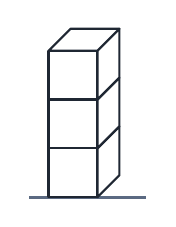
\begin{tikzpicture}[scale=0.62,line join=round]
  \draw[Slate,line width=1pt] (-0.4,0)--(2.0,0);
  \foreach \k/\f/\r in {0/4/1,1/5/3,2/3/1}{
    \begin{scope}[yshift=\k cm]
    \draw[Ink,line width=0.8pt,fill=white] (0,0) rectangle (1,1);
    \draw[Ink,line width=0.8pt,fill=white] (1,0)--(1.45,0.45)--(1.45,1.45)--(1,1)--cycle;
    \begin{scope}[Ink]\lgaPips{\f}\end{scope}
    \begin{scope}[Ink,cm={0.45,0.45,0,1,(1,0)}]\lgaPips{\r}\end{scope}
    \end{scope}}
  \draw[Ink,line width=0.8pt,fill=white] (0,3)--(1,3)--(1.45,3.45)--(0.45,3.45)--cycle;
  \begin{scope}[Ink,cm={1,0,0.45,0.45,(0,3)}]\lgaPips{2}\end{scope}
\end{tikzpicture}
\end{minipage}
\end{probbox}
\probsol{
\textbf{Phân tích đề.} Năm mặt bị che nằm ngang gồm: mặt đáy của con trên cùng; mặt trên và mặt đáy của con ở giữa; mặt trên và mặt đáy của
con dưới cùng. Ta không cần biết từng mặt có bao nhiêu chấm -- chỉ cần dùng ``hai mặt đối diện có tổng $7$''.
\begin{recallbox}Trên xúc xắc chuẩn, mặt trên và mặt đáy là hai mặt đối diện, nên tổng số chấm của chúng bằng $7$.\end{recallbox}
\step{1}{Con dưới cùng và con ở giữa}
Mỗi con có mặt trên và mặt đáy đều bị che, tổng mỗi cặp là $7$. Hai con: $7 + 7 = 14$.
\step{2}{Con trên cùng}
Mặt trên nhìn thấy có $2$ chấm, nên mặt đáy (đối diện) có $7 - 2 = 5$ chấm, và mặt này bị che.
\step{3}{Cộng lại}
$14 + 5 = 19$.
\begin{warnbox}(D) $21 = 3\times 7$ là quên rằng mặt trên cùng ($2$ chấm) \emph{nhìn thấy được}, không bị che. (A) $14$ là quên mặt đáy của con trên cùng
(cũng bị che, có $5$ chấm).\end{warnbox}
\verify{Sáu mặt nằm ngang của ba con có tổng $3\times 7 = 21$; trong đó chỉ mặt trên cùng ($2$ chấm) là nhìn thấy, nên năm mặt bị che có tổng $21 - 2 = 19$.}
Vậy chọn \textbf{(C)}.
\ans{(C) $19$}
}

% ---------------------------------------------------------------- Bài 27
\begin{probbox}{27}{\relax}
\begin{minipage}[t]{0.63\linewidth}
Lưới $4\times 4$ bên cạnh cần được điền sao cho mỗi hàng, mỗi cột và mỗi ô vuông $2\times 2$ viền đậm đều có đủ các chữ số $1, 2, 3, 4$.
Chữ số ở ô $Q$ là
\choicesL{$1$}{$2$}{$3$}{$4$}{Không xác định được}
\end{minipage}\hfill
\begin{minipage}[t]{0.33\linewidth}\vspace{4pt}\centering
\lgaFour{2/1/$3$,4/1/$2$,4/2/$1$,1/3/$4$,3/4/$2$,4/4/$Q$}
\end{minipage}
\end{probbox}
\probsol{
\textbf{Phân tích đề.} Ô $Q$ nằm ở hàng $4$, cột $4$ (góc dưới phải), thuộc ô $2\times 2$ dưới phải.
\begin{recallbox}Chữ số trong một ô phải khác mọi chữ số đã có trong hàng, cột và ô $2\times 2$ chứa nó.\end{recallbox}
\step{1}{Cột $4$}
Cột $4$ đã có $2$ (hàng $1$) và $1$ (hàng $2$). Hai ô còn lại -- hàng $3$ cột $4$ và ô $Q$ -- phải là $3$ và $4$ theo một thứ tự nào đó.
\step{2}{Hàng $3$ quyết định}
Hàng $3$ đã có chữ số $4$ (ở cột $1$), nên hàng $3$ cột $4$ \emph{không} thể là $4$. Vậy hàng $3$ cột $4$ là $3$, và $Q = 4$.
\step{3}{Kiểm tra với ô $2\times 2$ dưới phải và hàng $4$}
Ô $2\times 2$ dưới phải chứa $3$ (hàng $3$ cột $4$), $2$ (hàng $4$ cột $3$), $Q = 4$ và ô còn lại (hàng $3$ cột $3$) là $1$ -- đủ $1, 2, 3, 4$.
Hàng $4$ có $2$ và $4$, không lặp.
\step{4}{Hoàn thành lưới (để chắc chắn không mâu thuẫn)}
\begin{figC}
  \node at (0,0){\lgaFour{1/1/$1$,2/1/$3$,3/1/$4$,4/1/$2$,1/2/$2$,2/2/$4$,3/2/$3$,4/2/$1$,1/3/$4$,2/3/$2$,3/3/$1$,4/3/$3$,1/4/$3$,2/4/$1$,3/4/$2$,4/4/\textcolor{AnsRed}{$\mathbf{4}$}}};
  \node[font=\small,anchor=west,align=left] at (1.8,0){Hàng $1$: $1\,3\,4\,2$\\ Hàng $2$: $2\,4\,3\,1$\\ Hàng $3$: $4\,2\,1\,3$\\ Hàng $4$: $3\,1\,2\,4$};
\end{figC}
\verify{Mọi hàng, cột và ô $2\times 2$ đều có đủ $1, 2, 3, 4$; máy tính kiểm tra thấy lưới chỉ có duy nhất cách điền này.}
\begin{warnbox}Chỉ nhìn cột $4$ thì thấy $Q$ có thể là $3$ hoặc $4$ và dễ chọn (E). Hãy nhìn thêm hàng $3$ -- một vùng khác chứa ô ``hàng xóm'' của $Q$.\end{warnbox}
Vậy chọn \textbf{(D)}.
\ans{(D) $4$}
}

% ---------------------------------------------------------------- Bài 28
\begin{probbox}{28}{\relax}
Ở lớp 7A, \emph{tất cả} các bạn trong câu lạc bộ cờ vua đều biết bơi. Bạn Leo không biết bơi. Bạn Nora biết bơi. Khẳng định nào sau đây
\textbf{chắc chắn} đúng?
\choicesL{Leo ở trong câu lạc bộ cờ vua.}{Leo không ở trong câu lạc bộ cờ vua.}{Nora ở trong câu lạc bộ cờ vua.}{Nora không ở trong câu lạc bộ cờ vua.}{Mọi bạn biết bơi trong lớp đều ở câu lạc bộ cờ vua.}
\end{probbox}
\probsol{
\textbf{Phân tích đề.} Câu ``tất cả các bạn trong CLB cờ vua đều biết bơi'' có dạng ``mọi A đều là B'' (A: ở CLB cờ vua, B: biết bơi).
\begin{recallbox}Từ ``mọi A đều là B'' suy ra được ``không là B thì không là A''; nhưng \emph{không} suy ra được ``là B thì là A''.\end{recallbox}
\step{1}{Vẽ sơ đồ}
\begin{figC}
  \draw[tmBlue,line width=1pt,fill=tmBlue!8] (0.9,1.1) ellipse (1.9 and 1.2);
  \draw[tmOrange,line width=1pt,fill=tmOrange!15] (0.3,1.0) ellipse (0.95 and 0.7);
  \node[font=\scriptsize,text=tmOrange!70!black] at (0.3,1.3){CLB cờ vua};
  \node[font=\scriptsize,text=tmBlue!80!black] at (1.95,1.6){biết bơi};
  \fill[tmGreen!60!black] (1.95,0.95) circle (2.2pt) node[below,font=\scriptsize]{Nora?};
  \fill[tmGreen!60!black] (0.3,0.9) circle (2.2pt) node[below,font=\scriptsize]{Nora?};
  \fill[AnsRed] (3.6,1.1) circle (2.2pt) node[right,font=\scriptsize]{Leo};
\end{figC}
Vòng ``CLB cờ vua'' nằm trọn trong vòng ``biết bơi''.
\step{2}{Leo}
Leo không biết bơi, nên Leo nằm \emph{ngoài} vòng lớn, do đó chắc chắn nằm ngoài vòng nhỏ: \textbf{Leo không ở CLB cờ vua}. Nếu Leo ở CLB thì
Leo phải biết bơi -- trái với đề (phản chứng).
\step{3}{Nora}
Nora biết bơi: Nora nằm trong vòng lớn, nhưng có thể ở trong hoặc ngoài vòng nhỏ. Vậy (C) và (D) đều chỉ \emph{có thể} đúng, không chắc chắn.
\step{4}{Câu (E)}
(E) đảo ngược câu đề bài. Đề không nói gì về những bạn biết bơi nhưng không chơi cờ, nên (E) không chắc chắn đúng.
\begin{warnbox}Lỗi rất phổ biến: từ ``người chơi cờ đều biết bơi'' suy ra ``người biết bơi đều chơi cờ''. Hãy nghĩ một ví dụ: ``mọi con mèo đều có
bốn chân'' không có nghĩa ``mọi con vật bốn chân đều là mèo''!\end{warnbox}
Vậy chọn \textbf{(B)}.
\ans{(B) Leo không ở trong câu lạc bộ cờ vua}
}

% ---------------------------------------------------------------- Bài 29
\begin{probbox}{29}{\relax}
Chú Cáo nói dối vào các ngày thứ Hai, thứ Ba, thứ Tư và nói thật vào các ngày còn lại trong tuần. Một hôm, Cáo nói: ``Hôm qua tôi đã nói dối.''
Hôm đó có thể là ngày nào?
\choicesL{Chỉ có thể là thứ Hai.}{Chỉ có thể là thứ Năm.}{Thứ Hai hoặc thứ Năm.}{Thứ Tư hoặc thứ Năm.}{Chủ nhật hoặc thứ Hai.}
\end{probbox}
\probsol{
\textbf{Phân tích đề.} Cáo nói được câu ``Hôm qua tôi đã nói dối'' khi:
\begin{itemize}[leftmargin=1.4em,itemsep=0pt,topsep=1pt]
\item hôm nay nói thật và câu đúng: hôm nay thật, hôm qua dối; hoặc
\item hôm nay nói dối và câu sai: hôm nay dối, hôm qua thật.
\end{itemize}
Tức là: \textbf{hôm qua và hôm nay khác loại}.
\begin{recallbox}Hôm qua của thứ Hai là Chủ nhật (tuần quay vòng).\end{recallbox}
\step{1}{Lập bảng}
\begin{center}
\setlength{\tabcolsep}{4pt}
\begin{tabular}{|l|c|c|c|c|c|c|c|}
\hline
\rowcolor{tmBlue!10} Hôm nay & T2 & T3 & T4 & T5 & T6 & T7 & CN \\ \hline
Hôm nay Cáo & D & D & D & T & T & T & T \\ \hline
Hôm qua Cáo & T (CN) & D & D & D & T & T & T \\ \hline
Khác loại? & \textbf{có} & -- & -- & \textbf{có} & -- & -- & -- \\ \hline
\end{tabular}
\end{center}
\step{2}{Kiểm tra hai ngày tìm được}
\emph{Thứ Hai:} Cáo nói dối; hôm qua (Chủ nhật) Cáo nói thật, nên câu ``hôm qua tôi nói dối'' sai -- đúng là một lời nói dối. \checkmark\\
\emph{Thứ Năm:} Cáo nói thật; hôm qua (thứ Tư) Cáo nói dối, nên câu đó đúng -- đúng là lời nói thật. \checkmark
\begin{warnbox}Thứ Tư: Cáo nói dối, hôm qua (thứ Ba) cũng nói dối, nên câu ``hôm qua tôi đã nói dối'' là câu \emph{đúng}. Người đang nói dối không
nói câu đúng, nên thứ Tư bị loại -- đây là bẫy của phương án (D).\end{warnbox}
Vậy chọn \textbf{(C)}.
\ans{(C) Thứ Hai hoặc thứ Năm}
}

% ---------------------------------------------------------------- Bài 30
\begin{probbox}{30}{\relax}
Bốn bạn Amy, Ben, Chloe, David thi chạy, không có hai bạn nào về cùng lúc. Ba bạn đứng xem dự đoán:
\begin{itemize}[leftmargin=1.6em,itemsep=0pt,topsep=2pt]
\item Henry: ``Amy về nhất, Ben về nhì.''
\item Kate: ``Chloe về nhất, David về thứ tư.''
\item Lucy: ``Ben về thứ ba, David về nhì.''
\end{itemize}
Kết quả là mỗi bạn dự đoán đúng \emph{đúng một} ý. Hãy tìm thứ tự về đích của bốn bạn.
\end{probbox}
\probsol{
\textbf{Phân tích đề.} Mỗi dự đoán có hai ý, đúng một ý đúng. Ta xét trường hợp theo dự đoán của Henry.
\begin{recallbox}Câu ``đúng một nửa'': ý này đúng thì ý kia sai, ý này sai thì ý kia đúng.\end{recallbox}
\step{1}{Trường hợp 1: ``Ben về nhì'' đúng (và ``Amy về nhất'' sai)}
Xét dự đoán của Lucy. Ben về nhì nên ``Ben về thứ ba'' sai; vậy ý còn lại ``David về nhì'' phải đúng. Nhưng Ben đã về nhì, David không thể
cũng về nhì. \textbf{Mâu thuẫn} -- loại trường hợp này.
\step{2}{Trường hợp 2: ``Amy về nhất'' đúng (và ``Ben về nhì'' sai)}
\begin{itemize}[leftmargin=1.4em,itemsep=1pt,topsep=1pt]
\item Kate: Amy về nhất nên ``Chloe về nhất'' sai $\Rightarrow$ ``David về thứ tư'' đúng.
\item Lucy: David về thứ tư nên ``David về nhì'' sai $\Rightarrow$ ``Ben về thứ ba'' đúng.
\item Còn lại vị trí thứ nhì cho Chloe.
\end{itemize}
Thứ tự: Amy (nhất), Chloe (nhì), Ben (ba), David (tư).
\step{3}{Thử lại}
\begin{center}
\begin{tabular}{|l|c|c|}
\hline
\rowcolor{tmBlue!10} Người dự đoán & Ý thứ nhất & Ý thứ hai \\ \hline
Henry & Amy nhất: \textcolor{tmGreen!70!black}{đúng} & Ben nhì: \textcolor{AnsRed}{sai} \\ \hline
Kate & Chloe nhất: \textcolor{AnsRed}{sai} & David tư: \textcolor{tmGreen!70!black}{đúng} \\ \hline
Lucy & Ben ba: \textcolor{tmGreen!70!black}{đúng} & David nhì: \textcolor{AnsRed}{sai} \\ \hline
\end{tabular}
\end{center}
\begin{tipbox}Chọn dự đoán để xét trường hợp sao cho mỗi trường hợp ``kéo theo'' được nhiều ý khác. Ở đây ý ``Ben nhì'' va chạm ngay với
``David nhì'' của Lucy, nên trường hợp 1 bị loại rất nhanh.\end{tipbox}
\begin{parentbox}Có thể cùng con dùng bốn mẩu giấy ghi tên, xếp thành hàng ``nhất -- nhì -- ba -- tư'' và đổi chỗ để thử. Sau đó hỏi con:
``Mình có thử hết các trường hợp chưa? Làm sao chắc chắn không còn đáp án khác?'' -- câu trả lời chính là Bước 1.\end{parentbox}
\ans{Amy nhất, Chloe nhì, Ben ba, David tư.}
}

% ---------------- part c ----------------
% =====================================================================
% Chủ đề 5 — Tư duy logic và Câu đố — phần c: bài 31–40 (mở rộng)
% =====================================================================
% ---- helper macros for parts c/d of topic 5 (prefix \lgxcd, guarded) ----
% shape codes: 1 = circle, 2 = square, 3 = triangle, 4 = star
\providecommand{\lgxcdShape}[3]{\ifcase#1\or
  \draw[Ink,fill=Slate!35,line width=0.6pt] (#2,#3) circle (0.19);\or
  \draw[Ink,fill=tmBlue!35,line width=0.6pt] ($(#2,#3)+(-0.18,-0.18)$) rectangle ($(#2,#3)+(0.18,0.18)$);\or
  \draw[Ink,fill=tmOrange!45,line width=0.6pt] ($(#2,#3)+(-0.2,0.17)$)--($(#2,#3)+(0.2,0.17)$)--($(#2,#3)+(0,-0.19)$)--cycle;\or
  \draw[Ink,fill=tmGreen!45,line width=0.6pt,shift={(#2,#3)}] (90:0.24) \foreach \lgxcdk in {1,...,9}{ -- ({90+36*\lgxcdk}:{ifthenelse(mod(\lgxcdk,2)==1,0.1,0.24)})} -- cycle;\fi}
% inline shape in text
\providecommand{\lgxcdI}[1]{\tikz[baseline=-0.7ex]{\lgxcdShape{#1}{0}{0}}}
% a row of n shapes centred at the origin: \lgxcdRow{n}{codes}
\providecommand{\lgxcdRow}[2]{\foreach \lgxcdt [count=\lgxcdi] in {#2}{%
  \pgfmathsetmacro\lgxcdxx{(\lgxcdi-(#1+1)/2)*0.48}\lgxcdShape{\lgxcdt}{\lgxcdxx}{0.21}}}
% equal-arm balance at height #1: \lgxcdBal{y}{n left}{codes left}{n right}{codes right}
\providecommand{\lgxcdBal}[5]{\begin{scope}[yshift=#1cm]
  \draw[Ink,line width=1pt] (-2.7,0)--(-0.3,0) (0.3,0)--(2.7,0);
  \draw[Ink,line width=0.9pt] (-1.5,0)--(-1.5,-0.55)--(1.5,-0.55)--(1.5,0);
  \draw[Ink,fill=Slate!25,line width=0.9pt] (-0.22,-0.95)--(0,-0.55)--(0.22,-0.95)--cycle;
  \draw[Ink,line width=1pt] (-0.45,-0.95)--(0.45,-0.95);
  \begin{scope}[xshift=-1.5cm]\lgxcdRow{#2}{#3}\end{scope}
  \begin{scope}[xshift=1.5cm]\lgxcdRow{#4}{#5}\end{scope}\end{scope}}
% square grid n x n with box lines every #2 rows / #3 columns; #4 = given r/c/v, #5 = filled r/c/v (rows from top)
\providecommand{\lgxcdSud}[5]{\begin{scope}[x=0.62cm,y=0.62cm]
  \foreach \lgxcdi in {0,...,#1}{\draw[Slate!60,line width=0.5pt] (0,\lgxcdi)--(#1,\lgxcdi) (\lgxcdi,0)--(\lgxcdi,#1);}
  \foreach \lgxcdi in {0,#2,...,#1}{\draw[Ink,line width=1.4pt] (0,\lgxcdi)--(#1,\lgxcdi);}
  \foreach \lgxcdi in {0,#3,...,#1}{\draw[Ink,line width=1.4pt] (\lgxcdi,0)--(\lgxcdi,#1);}
  \foreach \lgxcdr/\lgxcdc/\lgxcdv in {#4}{\node[font=\sffamily\bfseries,text=Ink] at (\lgxcdc+0.5,#1-\lgxcdr-0.5){\lgxcdv};}
  \foreach \lgxcdr/\lgxcdc/\lgxcdv in {#5}{\node[font=\sffamily,text=tmBlue] at (\lgxcdc+0.5,#1-\lgxcdr-0.5){\lgxcdv};}
  \end{scope}}

\clearpage
\dividerbar{Mở rộng -- Nâng cao}

% ---------------------------------------------------------------- Bài 31

\begin{probbox}{31}{\relax}
Trên một hòn đảo, mỗi người dân hoặc là \emph{người nói thật} (luôn nói thật), hoặc là \emph{kẻ nói dối} (luôn nói dối).
\begin{enumerate}[label=\alph*),leftmargin=1.6em,itemsep=1pt,topsep=2pt]
  \item Em gặp hai người dân Kate và Leo. Kate nói: ``Cả hai chúng tôi đều là kẻ nói dối.'' Hỏi mỗi người thuộc loại nào?
  \item Em gặp ba người dân Anna, Ben và Chloe.\\
  Anna nói: ``Ben là kẻ nói dối.''\\
  Ben nói: ``Chloe là kẻ nói dối.''\\
  Chloe nói: ``Anna và Ben đều là kẻ nói dối.''\\
  Hỏi mỗi người thuộc loại nào?
\end{enumerate}
\end{probbox}
\probsol{
\textbf{Phân tích đề.} Mỗi người chỉ có hai khả năng. Cách làm chắc chắn nhất là \emph{giả sử} một khả năng, rồi xem các câu nói có
phù hợp với giả sử đó không. Nếu dẫn tới mâu thuẫn thì loại khả năng đó.
\begin{recallbox}Người nói thật nói câu nào thì câu đó \textbf{đúng}. Kẻ nói dối nói câu nào thì câu đó \textbf{sai}.
Như vậy, mỗi câu nói cho ta một ``phương trình'': \emph{câu nói đúng} $\Longleftrightarrow$ \emph{người nói là người nói thật}.\end{recallbox}
\par\smallskip\textbf{Câu a).}
\step{1}{Giả sử Kate là người nói thật}
Khi đó câu của Kate đúng, tức là Kate là kẻ nói dối -- trái với giả sử. Vậy Kate \textbf{không thể} là người nói thật.
\step{2}{Kate là kẻ nói dối}
Câu ``Cả hai chúng tôi đều là kẻ nói dối'' là câu sai. Câu này sai khi \emph{ít nhất một} người không phải kẻ nói dối. Kate đã
là kẻ nói dối, nên người còn lại -- Leo -- phải là người nói thật.
\begin{warnbox}Phủ định của ``cả hai đều nói dối'' \textbf{không phải} là ``cả hai đều nói thật'', mà là ``có ít nhất một người
nói thật''.\end{warnbox}
\par\smallskip\textbf{Câu b).}
\step{3}{Giả sử Anna là người nói thật}
Câu của Anna đúng $\Rightarrow$ Ben là kẻ nói dối $\Rightarrow$ câu của Ben sai $\Rightarrow$ Chloe là người nói thật
$\Rightarrow$ câu của Chloe đúng $\Rightarrow$ Anna là kẻ nói dối. Trái với giả sử! Loại.
\step{4}{Vậy Anna là kẻ nói dối}
Câu của Anna sai $\Rightarrow$ Ben \emph{không} nói dối, tức Ben là người nói thật $\Rightarrow$ câu của Ben đúng
$\Rightarrow$ Chloe là kẻ nói dối.
\step{5}{Kiểm tra câu của Chloe}
Chloe là kẻ nói dối nên câu ``Anna và Ben đều là kẻ nói dối'' phải sai. Thật vậy, câu đó sai vì Ben là người nói thật.
Không có mâu thuẫn nào.
\begin{center}
\begin{tabular}{|c|c|l|c|}
\hline
\rowcolor{tmBlue!10} Người & Loại & Câu nói & Câu nói đúng/sai\\ \hline
Anna & nói dối & Ben là kẻ nói dối & sai \\ \hline
Ben & nói thật & Chloe là kẻ nói dối & đúng\\ \hline
Chloe & nói dối & Anna và Ben đều nói dối & sai\\ \hline
\end{tabular}
\end{center}
\verify{Trong bảng, mỗi người nói thật nói câu đúng, mỗi kẻ nói dối nói câu sai. Ta cũng đã thấy khả năng ``Anna nói thật''
bị loại, nên đây là lời giải duy nhất.}
\ans{a) Kate nói dối, Leo nói thật;\quad b) Anna và Chloe nói dối, Ben nói thật}
}

% ---------------------------------------------------------------- Bài 32

\begin{probbox}{32}{\relax}
Bạn Mia nói dối vào các ngày thứ Hai, thứ Ba, thứ Tư và nói thật vào những ngày còn lại trong tuần. Bạn Henry nói dối vào các ngày
thứ Năm, thứ Sáu, thứ Bảy và nói thật vào những ngày còn lại. Một hôm, cả hai bạn đều nói: ``Hôm qua là ngày tôi nói dối.''
Hỏi hôm đó là thứ mấy?
\end{probbox}
\probsol{
\textbf{Phân tích đề.} Câu nói ``Hôm qua là ngày tôi nói dối'' có thể đúng hoặc sai, tuỳ theo ngày. Với từng bạn, ta tìm những ngày
bạn đó \emph{có thể} nói câu này, rồi lấy ngày chung của hai bạn.
\begin{recallbox}Vào ngày nói thật, câu nói phải đúng; vào ngày nói dối, câu nói phải sai.\end{recallbox}
\step{1}{Lập bảng cho Mia (nói dối T2, T3, T4)}
\begin{center}\small
\begin{tabular}{|l|c|c|c|c|c|c|c|}
\hline
\rowcolor{tmBlue!10} Hôm nay & T2 & T3 & T4 & T5 & T6 & T7 & CN\\ \hline
Hôm nay Mia & dối & dối & dối & thật & thật & thật & thật\\ \hline
Hôm qua Mia & thật (CN) & dối & dối & dối & thật & thật & thật\\ \hline
Câu nói đúng? & sai & đúng & đúng & đúng & sai & sai & sai\\ \hline
Mia nói được? & \textbf{có} & không & không & \textbf{có} & không & không & không\\ \hline
\end{tabular}
\end{center}
Mia nói được câu này khi: hôm nay nói dối và câu sai (thứ Hai), hoặc hôm nay nói thật và câu đúng (thứ Năm).
\step{2}{Lập bảng cho Henry (nói dối T5, T6, T7)}
\begin{center}\small
\begin{tabular}{|l|c|c|c|c|c|c|c|}
\hline
\rowcolor{tmBlue!10} Hôm nay & T2 & T3 & T4 & T5 & T6 & T7 & CN\\ \hline
Hôm nay Henry & thật & thật & thật & dối & dối & dối & thật\\ \hline
Hôm qua Henry & thật & thật & thật & thật & dối & dối & dối\\ \hline
Câu nói đúng? & sai & sai & sai & sai & đúng & đúng & đúng\\ \hline
Henry nói được? & không & không & không & \textbf{có} & không & không & \textbf{có}\\ \hline
\end{tabular}
\end{center}
Henry nói được câu này vào thứ Năm hoặc Chủ nhật.
\step{3}{Ngày chung}
Mia: $\{$thứ Hai, thứ Năm$\}$; Henry: $\{$thứ Năm, Chủ nhật$\}$. Ngày chung duy nhất là \textbf{thứ Năm}.
\begin{tipbox}Quy luật nhanh: người này chỉ nói được câu ``Hôm qua tôi nói dối'' vào ngày \emph{chuyển chế độ}
(hôm qua và hôm nay khác chế độ): ngày đầu tiên nói dối, hoặc ngày đầu tiên nói thật trở lại.\end{tipbox}
\verify{Thứ Năm: Mia nói thật, hôm qua (thứ Tư) Mia nói dối -- câu đúng, hợp lí. Henry nói dối, hôm qua (thứ Tư) Henry nói thật --
câu sai, hợp lí với việc Henry đang nói dối.}
\ans{Thứ Năm}
}

% ---------------------------------------------------------------- Bài 33

\begin{probbox}{33}{\relax}
Sáu bạn Lucy, Max, Noah, Olivia, Peter và Quinn chạy thi. Không có hai bạn nào về đích cùng lúc. Biết rằng:
\begin{itemize}[leftmargin=1.4em,itemsep=0pt,topsep=2pt]
  \item Max về đích sau Lucy nhưng trước Noah;
  \item Olivia về đích sau Noah;
  \item Peter về đích \emph{ngay sau} Lucy;
  \item Quinn không về nhất cũng không về bét, và Quinn về trước Max.
\end{itemize}
Hãy xếp thứ tự về đích của sáu bạn. Ai về thứ ba?
\end{probbox}
\probsol{
\textbf{Phân tích đề.} Ta có các điều kiện ``trước -- sau''. Cách hay là ghép chúng thành một \emph{chuỗi} rồi chèn dần những
bạn còn lại vào. Viết $X \to Y$ nghĩa là ``$X$ về trước $Y$''.
\step{1}{Ghép điều kiện 1 và 2}
Lucy $\to$ Max $\to$ Noah và Noah $\to$ Olivia, nên: \ Lucy $\to$ Max $\to$ Noah $\to$ Olivia.
\step{2}{Chèn Peter}
Peter về \emph{ngay sau} Lucy, tức là không ai chen giữa Lucy và Peter: \ Lucy, Peter $\to$ Max $\to$ Noah $\to$ Olivia.
\step{3}{Chèn Quinn}
Quinn về trước Max, nên Quinn đứng ở một trong các chỗ: trước Lucy, hoặc giữa Peter và Max (không được chen giữa Lucy và Peter).
Nhưng Quinn không về nhất, nên Quinn không đứng trước Lucy. Vậy:
\[ \text{Lucy} \to \text{Peter} \to \text{Quinn} \to \text{Max} \to \text{Noah} \to \text{Olivia}. \]
\begin{figC}
\foreach \n/\x in {Lucy/0,Peter/1,Quinn/2,Max/3,Noah/4,Olivia/5}{
  \node[draw=tmBlue,fill=tmBlue!8,rounded corners=3pt,minimum width=1.5cm,minimum height=0.7cm] at (\x*1.9,0){\n};}
\foreach \x [count=\k] in {0,...,5}{\node[font=\scriptsize,text=Slate] at (\x*1.9,-0.6){hạng \k};}
\foreach \x in {0,...,4}{\draw[->,tmBlue,thick] (\x*1.9+0.78,0)--(\x*1.9+1.12,0);}
\end{figC}
\step{4}{Kiểm tra lại từng điều kiện}
Max (hạng 4) sau Lucy (hạng 1), trước Noah (hạng 5): đúng. Olivia (hạng 6) sau Noah: đúng. Peter (hạng 2) ngay sau Lucy: đúng.
Quinn hạng 3 -- không nhất, không bét, trước Max: đúng.
\begin{warnbox}Nếu quên chữ ``ngay sau'' thì Quinn có thể chen giữa Lucy và Peter, và bài toán sẽ có hai đáp án. Hãy đọc kĩ từng chữ
của điều kiện!\end{warnbox}
\verify{Đã thử mọi vị trí có thể của Quinn; chỉ có một thứ tự thoả mãn cả bốn điều kiện.}
\ans{Lucy, Peter, Quinn, Max, Noah, Olivia; Quinn về thứ ba}
}

% ---------------------------------------------------------------- Bài 34

\begin{probbox}{34}{\relax}
Năm bạn Hannah, Kevin, Lily, Maya và Tom ngồi trên một hàng ghế gồm $5$ ghế đánh số $1, 2, 3, 4, 5$ từ trái sang phải. Biết rằng:
Hannah và Kevin ngồi cạnh nhau; Lily và Maya \emph{không} ngồi cạnh nhau; Tom ngồi ở một đầu hàng ghế (ghế $1$ hoặc ghế $5$).
\begin{enumerate}[label=\alph*),leftmargin=1.6em,itemsep=1pt,topsep=2pt]
  \item Có tất cả bao nhiêu cách ngồi thoả mãn các điều kiện trên?
  \item Trong các khẳng định sau, khẳng định nào \emph{chắc chắn đúng}?\\
  (1) Lily ngồi ở một đầu hàng ghế.\\
  (2) Hannah không ngồi ở đầu hàng ghế.\\
  (3) Kevin ngồi ở ghế số $3$.
  \item Nếu biết thêm Lily ngồi ghế số $1$ và Hannah ngồi bên trái Kevin, hãy xác định chỗ ngồi của từng bạn.
\end{enumerate}
\end{probbox}
\probsol{
\textbf{Phân tích đề.} Bắt đầu từ điều kiện ``chặt'' nhất (Tom chỉ có $2$ chỗ), rồi xét $4$ ghế còn lại.
\step{1}{Xét trường hợp Tom ngồi ghế 5}
Bốn bạn còn lại ngồi ghế $1, 2, 3, 4$. Cặp Hannah -- Kevin chiếm hai ghế liền nhau: ghế $(1,2)$, $(2,3)$ hoặc $(3,4)$.
\begin{itemize}[leftmargin=1.4em,itemsep=0pt,topsep=1pt]
  \item Hannah -- Kevin ở ghế $(1,2)$: Lily, Maya phải ngồi ghế $3, 4$ -- cạnh nhau, \textbf{loại}.
  \item Hannah -- Kevin ở ghế $(3,4)$: Lily, Maya ngồi ghế $1, 2$ -- cạnh nhau, \textbf{loại}.
  \item Hannah -- Kevin ở ghế $(2,3)$: Lily, Maya ngồi ghế $1$ và $4$ -- không cạnh nhau, \textbf{được}.
\end{itemize}
Trong trường hợp được: Hannah, Kevin đổi chỗ cho nhau được ($2$ cách), Lily, Maya đổi chỗ cho nhau được ($2$ cách):
$2\times 2 = 4$ cách.
\step{2}{Trường hợp Tom ngồi ghế 1}
Hoàn toàn tương tự (lật ngược hàng ghế): Hannah -- Kevin ở ghế $(3,4)$, Lily và Maya ở ghế $2$ và $5$: cũng $4$ cách.
\step{3}{Tổng số cách}
$4 + 4 = 8$ cách.
\begin{recallbox}\textbf{Quy tắc nhân:} nếu một việc gồm các bước liên tiếp, bước 1 có $m$ cách, bước 2 có $n$ cách, thì cả việc có
$m\times n$ cách. \textbf{Quy tắc cộng:} các trường hợp tách rời nhau thì cộng số cách.\end{recallbox}
\needspace{7\baselineskip}\step{4}{Câu b): kiểm tra từng khẳng định}
\begin{center}\small
\begin{tabular}{|c|c|c|c|c|}
\hline
\rowcolor{tmBlue!10} Ghế 1 & Ghế 2 & Ghế 3 & Ghế 4 & Ghế 5\\ \hline
Lily/Maya & Hannah/Kevin & Hannah/Kevin & Maya/Lily & Tom\\ \hline
Tom & Lily/Maya & Hannah/Kevin & Hannah/Kevin & Maya/Lily\\ \hline
\end{tabular}
\end{center}
(1) Sai: khi Tom ngồi ghế 1, Lily có thể ngồi ghế 2. \ (2) \textbf{Đúng}: trong cả hai dòng, Hannah và Kevin luôn ở các ghế giữa
($2, 3$ hoặc $3, 4$). \ (3) Sai: Kevin có thể ngồi ghế $2$ hoặc ghế $4$.
\step{5}{Câu c)}
Lily ngồi ghế $1$ nên Tom không ở ghế $1$, vậy Tom ở ghế $5$ (dòng thứ nhất của bảng). Khi đó Maya ở ghế $4$, Hannah -- Kevin ở ghế $2, 3$;
Hannah bên trái Kevin nên Hannah ghế $2$, Kevin ghế $3$.
\verify{Lily(1), Hannah(2), Kevin(3), Maya(4), Tom(5): Hannah -- Kevin cạnh nhau; Lily ghế 1 và Maya ghế 4 không cạnh nhau; Tom ở đầu hàng.
Đúng.}
\ans{a) $8$ cách;\quad b) khẳng định (2);\quad c) Lily -- Hannah -- Kevin -- Maya -- Tom (ghế 1 đến 5)}
}

% ---------------------------------------------------------------- Bài 35

\begin{probbox}{35}{\relax}
Đánh số các chữ cái $A, B, C, \dots, Z$ (bảng chữ cái tiếng Anh, $26$ chữ) lần lượt là $0, 1, 2, \dots, 25$. \emph{Mật mã Caesar
với khoá $k$} thay mỗi chữ cái mang số $x$ bằng chữ cái mang số là \emph{số dư} của $x + k$ khi chia cho $26$
(dấu cách giữ nguyên).
\begin{figC}
\foreach \L [count=\i from 0] in {A,B,C,D,E,F,G,H,I,J,K,L,M,N,O,P,Q,R,S,T,U,V,W,X,Y,Z}{
  \node[font=\sffamily\small\bfseries,text=Ink] at ({90-\i*360/26}:2.15){\L};
  \node[font=\sffamily\tiny,text=tmBlue] at ({90-\i*360/26}:1.65){\i};}
\draw[Line,line width=0.8pt] (0,0) circle (1.9);
\draw[->,tmOrange,line width=1pt] (110:1.2) arc (110:30:1.2);
\node[font=\scriptsize,text=tmOrange!80!black,align=center] at (0,0){đi theo\\chiều kim\\đồng hồ};
\end{figC}
\begin{enumerate}[label=\alph*),leftmargin=1.6em,itemsep=1pt,topsep=2pt]
  \item Mã hoá dòng chữ \textsf{MATH CLUB} với khoá $k = 5$.
  \item Giải mã dòng chữ \textsf{FVB DPU}, biết khoá là $k = 7$.
  \item Một tin nhắn có từ \textsf{CAT} được mã hoá thành \textsf{RPI}. Tìm khoá $k$ (với $0 \le k \le 25$), rồi giải mã từ
  \textsf{SDV} của cùng tin nhắn.
  \item Mã hoá một tin với khoá $10$, rồi mã hoá kết quả thêm một lần nữa với khoá $20$. Hai lần mã hoá đó giống với
  \emph{một} lần mã hoá với khoá nào?
  \item Bạn Sam mã hoá một từ với khoá $4$, rồi lại mã hoá kết quả với khoá $4$, cứ thế nhiều lần. Sau ít nhất bao nhiêu lần
  thì Sam lại thu được đúng từ ban đầu?
\end{enumerate}
\end{probbox}
\probsol{
\textbf{Phân tích đề.} Khi cộng khoá mà vượt quá $25$, ta ``quay vòng'' về đầu bảng chữ cái -- đó chính là lấy \emph{số dư khi
chia cho $26$}. Giải mã là làm ngược lại: \emph{trừ} khoá (nếu ra số âm thì cộng thêm $26$).
\begin{recallbox}Số dư của $a$ khi chia cho $26$ là số $r$ với $0 \le r \le 25$ sao cho $a - r$ chia hết cho $26$.
Ví dụ: $30$ chia $26$ dư $4$; \ $-6$ ``chia $26$ dư'' $20$ vì $-6 + 26 = 20$.\end{recallbox}
\step{1}{Câu a): mã hoá \textsf{MATH CLUB} với $k = 5$}
\begin{center}\small
\begin{tabular}{|c|c|c|c|c|c|c|c|c|}
\hline
\rowcolor{tmBlue!10} Chữ gốc & M & A & T & H & C & L & U & B\\ \hline
Số $x$ & $12$ & $0$ & $19$ & $7$ & $2$ & $11$ & $20$ & $1$\\ \hline
$x + 5$ & $17$ & $5$ & $24$ & $12$ & $7$ & $16$ & $25$ & $6$\\ \hline
Chữ mã & R & F & Y & M & H & Q & Z & G\\ \hline
\end{tabular}
\end{center}
Kết quả: \textsf{RFYM HQZG}. (Ở đây không có số nào vượt $25$ nên chưa cần quay vòng.)
\step{2}{Câu b): giải mã \textsf{FVB DPU} với $k = 7$ (trừ $7$)}
\begin{center}\small
\begin{tabular}{|c|c|c|c|c|c|c|}
\hline
\rowcolor{tmBlue!10} Chữ mã & F & V & B & D & P & U\\ \hline
Số & $5$ & $21$ & $1$ & $3$ & $15$ & $20$\\ \hline
Số $- 7$ & $-2 \to 24$ & $14$ & $-6 \to 20$ & $-4 \to 22$ & $8$ & $13$\\ \hline
Chữ gốc & Y & O & U & W & I & N\\ \hline
\end{tabular}
\end{center}
Tin gốc: \textsf{YOU WIN} (tiếng Anh: ``Bạn thắng rồi''). Chú ý: các chữ F, B, D mang số nhỏ hơn $7$ nên khi trừ $7$ ta được số âm,
phải cộng thêm $26$; ví dụ $5 - 7 = -2$, $-2 + 26 = 24$ (chữ Y).
\step{3}{Câu c): tìm khoá từ cặp \textsf{CAT} $\to$ \textsf{RPI}}
C ($2$) thành R ($17$), nên $k = 17 - 2 = 15$. Kiểm tra: A ($0$) $\to 0 + 15 = 15$ (P) đúng; T ($19$) $\to 19 + 15 = 34$,
chia $26$ dư $8$ (I) đúng. Vậy $k = 15$.\\
Giải mã \textsf{SDV} (trừ $15$): S $= 18$, $18 - 15 = 3$ (D); \ D $= 3$, $3 - 15 = -12 \to 14$ (O); \ V $= 21$, $21 - 15 = 6$ (G).
Từ gốc là \textsf{DOG}.
\step{4}{Câu d): hai lần mã hoá liên tiếp}
Mỗi chữ được cộng $10$ rồi cộng $20$, tức là cộng $30$. Vì $30$ chia $26$ dư $4$, nên ``cộng $30$ rồi lấy dư'' giống hệt
``cộng $4$ rồi lấy dư''. Hai lần mã hoá giống \textbf{một lần mã hoá với khoá $4$}.
\step{5}{Câu e): mã hoá lặp lại với khoá $4$}
Sau $n$ lần, mỗi chữ đã bị dịch đi $4n$ vị trí. Muốn quay về đúng chữ ban đầu thì phải đi trọn một số vòng, tức $4n$ chia hết
cho $26$. Thử $n = 1, 2, 3, \dots$: \ $4n = 4, 8, 12, \dots$ Số $4n$ nhỏ nhất (khác $0$) chia hết cho $26$ là
$\text{BCNN}(4, 26) = 52$, ứng với $n = 52 : 4 = 13$.
\begin{recallbox}$4n$ chia hết cho $26 = 2\times 13$ $\Leftrightarrow$ $2n$ chia hết cho $13$ $\Leftrightarrow$ $n$ chia hết cho $13$
(vì $13$ là số nguyên tố không chia hết $2$).\end{recallbox}
\begin{tipbox}Với khoá $13$ thì chỉ cần mã hoá $2$ lần là về chỗ cũ ($2\times 13 = 26$). Vì vậy với khoá $13$,
giải mã cũng chính là mã hoá thêm một lần nữa!\end{tipbox}
\needspace{5\baselineskip}\verify{Câu a): giải mã \textsf{RFYM HQZG} bằng cách trừ $5$ được lại \textsf{MATH CLUB}. Câu c): \textsf{DOG} mã hoá với khoá
$15$: D $3 + 15 = 18$ (S), O $14 + 15 = 29 \to 3$ (D), G $6 + 15 = 21$ (V). Đúng \textsf{SDV}.}
\ans{a) \textsf{RFYM HQZG};\ b) \textsf{YOU WIN};\ c) $k = 15$, \textsf{DOG};\ d) khoá $4$;\ e) $13$ lần}
}

% ---------------------------------------------------------------- Bài 36

\begin{probbox}{36}{\stars{1}}
Vẫn đánh số $A = 0, B = 1, \dots, Z = 25$. Một \emph{mật mã nhân} thay chữ cái mang số $x$ bằng chữ cái mang số là
số dư của $3x + 2$ khi chia cho $26$.
\begin{enumerate}[label=\alph*),leftmargin=1.6em,itemsep=1pt,topsep=2pt]
  \item Mã hoá từ \textsf{MAP}.
  \item Giải mã từ \textsf{EGW}.
  \item Bạn Nathan đề nghị dùng $2x + 2$ thay cho $3x + 2$. Hãy chỉ ra hai chữ cái khác nhau có cùng một chữ mã. Vì sao như vậy thì
  không giải mã được?
  \item Giải thích vì sao với $3x + 2$, hai chữ cái khác nhau luôn có hai chữ mã khác nhau.
\end{enumerate}
\end{probbox}
\probsol{
\textbf{Phân tích đề.} Mật mã này không chỉ ``dịch'' mà còn ``nhân'' rồi lấy số dư. Mã hoá thì dễ (tính thẳng); giải mã thì cần
tìm $x$ khi biết số dư của $3x + 2$ -- ta dùng cách ``thêm $26$ cho tới khi chia hết cho $3$''.
\step{1}{Câu a): mã hoá \textsf{MAP}}
M $= 12$: $3\cdot 12 + 2 = 38$, chia $26$ dư $12$ $\to$ M.\\
A $= 0$: $3\cdot 0 + 2 = 2$ $\to$ C.\\
P $= 15$: $3\cdot 15 + 2 = 47$, chia $26$ dư $21$ $\to$ V.\\
Kết quả: \textsf{MCV}. (Thú vị: chữ M được mã hoá thành chính nó.)
\step{2}{Câu b): giải mã \textsf{EGW}}
Với chữ mã mang số $y$, ta cần $x$ ($0 \le x \le 25$) sao cho $3x + 2$ chia $26$ dư $y$, tức là $3x = y - 2$, hoặc
$y - 2 + 26$, hoặc $y - 2 + 52$ (thử lần lượt, lấy số chia hết cho $3$).
\begin{center}\small
\begin{tabular}{|c|c|c|c|c|}
\hline
\rowcolor{tmBlue!10} Chữ mã & $y$ & Thử $y - 2,\ y + 24,\ y + 50$ & $3x$ & Chữ gốc\\ \hline
E & $4$ & $2$ (không), $28$ (không), $54$ (chia hết) & $54 \Rightarrow x = 18$ & S\\ \hline
G & $6$ & $4$ (không), $30$ (chia hết) & $30 \Rightarrow x = 10$ & K\\ \hline
W & $22$ & $20$ (không), $46$ (không), $72$ (chia hết) & $72 \Rightarrow x = 24$ & Y\\ \hline
\end{tabular}
\end{center}
Từ gốc là \textsf{SKY} (tiếng Anh: ``bầu trời'').
\step{3}{Câu c): vì sao $2x + 2$ không dùng được}
A $= 0$: $2\cdot 0 + 2 = 2$ $\to$ C. \quad N $= 13$: $2\cdot 13 + 2 = 28$, chia $26$ dư $2$ $\to$ C.\\
Hai chữ A và N cùng thành chữ C. Khi nhận được chữ C, người giải mã không biết chữ gốc là A hay N, nên không giải mã chắc chắn
được. (Thực ra mọi số $2x + 2$ đều chẵn, nên chỉ có $13$ chữ mã cho $26$ chữ gốc -- chắc chắn có các cặp trùng nhau.)
\step{4}{Câu d): vì sao $3x + 2$ không bị trùng}
\begin{proofbox}Giả sử hai chữ $x$ và $z$ (với $0 \le z < x \le 25$) có cùng chữ mã. Khi đó $3x + 2$ và $3z + 2$ có cùng số dư khi
chia cho $26$, nên hiệu của chúng $3(x - z)$ chia hết cho $26$. Nhưng $3$ và $26$ không có ước chung nào lớn hơn $1$, nên
$x - z$ phải chia hết cho $26$. Mà $0 < x - z \le 25$ -- không thể chia hết cho $26$. Mâu thuẫn. Vậy hai chữ khác nhau luôn có chữ
mã khác nhau.\end{proofbox}
\begin{warnbox}Với $2x + 2$, lập luận trên hỏng ở chỗ: $2(x - z)$ chia hết cho $26$ chỉ cần $x - z$ chia hết cho $13$, ví dụ
$x - z = 13$ (A và N).\end{warnbox}
\verify{Mã hoá lại \textsf{SKY}: S $3\cdot 18 + 2 = 56 \to 56 - 52 = 4$ (E); K $3\cdot 10 + 2 = 32 \to 6$ (G); Y $3\cdot 24 + 2 = 74 \to 74 - 52 = 22$ (W). Được
\textsf{EGW}, đúng.}
\ans{a) \textsf{MCV};\ b) \textsf{SKY};\ c) A và N đều thành C;\ d) xem chứng minh}
}

% ---------------------------------------------------------------- Bài 37

\begin{probbox}{37}{\relax}
Trong một \emph{ma phương} $3\times 3$, tổng các số trên mỗi hàng, mỗi cột và mỗi đường chéo đều bằng nhau (gọi là
\emph{tổng ma phương} $M$).
\begin{enumerate}[label=\alph*),leftmargin=1.6em,itemsep=1pt,topsep=2pt]
  \item Gọi $c$ là số ở ô chính giữa. Chứng minh rằng $M = 3c$.
  \item Điền nốt các ô trống của ma phương dưới đây.
\end{enumerate}
\begin{figC}
\lgxcdSud{3}{3}{3}{0/0/9,0/1/19,2/2/13}{}
\end{figC}
\end{probbox}
\probsol{
\textbf{Phân tích đề.} Ở câu b) chỉ biết ba số, không có số ở giữa và cũng không biết $M$. Câu a) chính là ``chìa khoá'': nó liên
hệ số ở giữa với $M$.
\step{1}{Câu a): cộng bốn đường đi qua ô giữa}
Đặt tên các ô:
\begin{figC}
\lgxcdSud{3}{3}{3}{0/0/$a$,0/1/$b$,0/2/$d$,1/0/$e$,1/1/$c$,1/2/$f$,2/0/$g$,2/1/$h$,2/2/$i$}{}
\end{figC}
Có bốn đường đi qua ô giữa: hàng giữa $e + c + f$, cột giữa $b + c + h$, hai đường chéo $a + c + i$ và $d + c + g$. Cộng bốn
tổng này:
\[ (e + c + f) + (b + c + h) + (a + c + i) + (d + c + g) = 4M. \]
Vế trái chứa mỗi ô ngoài đúng \emph{một} lần, còn ô giữa $c$ xuất hiện \emph{bốn} lần. Vậy vế trái bằng
(tổng cả $9$ ô) $+\, 3c$.
\begin{proofbox}Tổng cả $9$ ô bằng tổng của ba hàng, tức $3M$. Do đó $3M + 3c = 4M$, suy ra $3c = M$.\end{proofbox}
\step{2}{Câu b): tìm số ở giữa}
Đường chéo chính đi qua $9$, ô giữa $c$ và $13$: \ $9 + c + 13 = M = 3c$. Suy ra $22 = 2c$, $c = 11$ và $M = 33$.
\step{3}{Điền lần lượt các ô (mỗi lần chọn một đường chỉ còn thiếu một ô)}
\begin{itemize}[leftmargin=1.4em,itemsep=0pt,topsep=1pt]
  \item Hàng trên: $33 - 9 - 19 = 5$ (góc trên phải).
  \item Đường chéo phụ: $33 - 5 - 11 = 17$ (góc dưới trái).
  \item Cột trái: $33 - 9 - 17 = 7$; \quad hàng giữa: $33 - 7 - 11 = 15$.
  \item Hàng dưới: $33 - 17 - 13 = 3$.
\end{itemize}
\begin{figC}
\lgxcdSud{3}{3}{3}{0/0/9,0/1/19,2/2/13}{0/2/5,1/0/7,1/1/11,1/2/15,2/0/17,2/1/3}
\end{figC}
\verify{Cột giữa $19 + 11 + 3 = 33$; cột phải $5 + 15 + 13 = 33$; hàng giữa $7 + 11 + 15 = 33$; hai đường chéo $9 + 11 + 13$ và
$5 + 11 + 17$ đều bằng $33$.}
\begin{tipbox}Kết quả $M = 3c$ đúng với \emph{mọi} ma phương $3\times 3$, kể cả khi có số âm hay phân số.\end{tipbox}
\ans{a) xem chứng minh;\quad b) hàng trên $9, 19, 5$; hàng giữa $7, 11, 15$; hàng dưới $17, 3, 13$}
}

% ---------------------------------------------------------------- Bài 38

\begin{probbox}{38}{\relax}
Ba chiếc cân hai đĩa dưới đây đều thăng bằng. Các vật cùng hình dạng thì nặng bằng nhau.
\begin{figC}
\lgxcdBal{0}{2}{2,3}{5}{1,1,1,1,1}
\lgxcdBal{-1.7}{2}{3,3}{4}{1,1,1,1}
\lgxcdBal{-3.4}{2}{4,1}{2}{2,2}
\node[font=\small\bfseries,text=Slate] at (-3.3,0){(1)};
\node[font=\small\bfseries,text=Slate] at (-3.3,-1.7){(2)};
\node[font=\small\bfseries,text=Slate] at (-3.3,-3.4){(3)};
\end{figC}
\begin{enumerate}[label=\alph*),leftmargin=1.6em,itemsep=1pt,topsep=2pt]
  \item Mỗi vật \lgxcdI{3}, \lgxcdI{2}, \lgxcdI{4} nặng bằng bao nhiêu vật \lgxcdI{1}?
  \item Cần bao nhiêu vật \lgxcdI{3} để cân bằng với \lgxcdI{4}\,\lgxcdI{4}\,\lgxcdI{2}\,\lgxcdI{2}?
  \item Biết mỗi vật \lgxcdI{1} nặng $12$ g. Ba vật \lgxcdI{4}\,\lgxcdI{3}\,\lgxcdI{2} nặng tất cả bao nhiêu gam?
\end{enumerate}
\end{probbox}
\probsol{
\textbf{Phân tích đề.} Mỗi chiếc cân thăng bằng cho ta một \emph{đẳng thức}. Ta đặt ẩn cho khối lượng của từng loại vật, viết ba
đẳng thức, rồi giải lần lượt từ đẳng thức đơn giản nhất (chỉ chứa hai loại vật).
\begin{recallbox}Cân thăng bằng giống như một đẳng thức: khối lượng đĩa trái $=$ khối lượng đĩa phải. Ta được phép cộng (hoặc trừ)
cùng một lượng vào hai vế, hay chia hai vế cho cùng một số khác $0$ -- đẳng thức vẫn đúng (cũng như cân vẫn thăng bằng).\end{recallbox}
\step{1}{Đặt ẩn và viết các đẳng thức}
Gọi khối lượng mỗi vật \lgxcdI{1} (tròn), \lgxcdI{2} (vuông), \lgxcdI{3} (tam giác), \lgxcdI{4} (sao) lần lượt là $o$, $v$, $t$, $s$.
Đọc ba chiếc cân:
\[ \text{(1)}\ \ v + t = 5o; \qquad \text{(2)}\ \ 2t = 4o; \qquad \text{(3)}\ \ s + o = 2v. \]
\step{2}{Từ đẳng thức (2): tìm $t$}
Chia hai vế của $2t = 4o$ cho $2$: \ $t = 2o$. Vậy mỗi \lgxcdI{3} nặng bằng $2$ vật \lgxcdI{1}.
\step{3}{Thay vào đẳng thức (1): tìm $v$}
Thay $t = 2o$ vào (1): \ $v + 2o = 5o$. Trừ hai vế cho $2o$: \ $v = 5o - 2o = 3o$. Mỗi \lgxcdI{2} nặng bằng $3$ vật \lgxcdI{1}.
\step{4}{Thay vào đẳng thức (3): tìm $s$}
Thay $v = 3o$ vào (3): \ $s + o = 2\cdot 3o = 6o$. Trừ hai vế cho $o$: \ $s = 6o - o = 5o$. Mỗi \lgxcdI{4} nặng bằng $5$ vật
\lgxcdI{1}.
\step{5}{Câu b)}
Bốn vật \lgxcdI{4}\,\lgxcdI{4}\,\lgxcdI{2}\,\lgxcdI{2} nặng $2s + 2v = 2\cdot 5o + 2\cdot 3o = 10o + 6o = 16o$.\\
Gọi $n$ là số vật \lgxcdI{3} cần dùng. Ta cần $n\cdot t = 16o$, tức là $n\cdot 2o = 16o$, suy ra $n = 16 : 2 = 8$.
\step{6}{Câu c)}
Với $o = 12$ g: \ $s + t + v = 5o + 2o + 3o = 10o = 10\cdot 12 = 120$ (g).
\verify{Với $o = 1$, $t = 2$, $v = 3$, $s = 5$: cân (1) $3 + 2 = 5$; cân (2) $2\cdot 2 = 4$; cân (3) $5 + 1 = 6 = 2\cdot 3$.
Cả ba cân đều thăng bằng. Câu b): $8$ tam giác nặng $8\cdot 2 = 16$, đúng bằng $5 + 5 + 3 + 3$.}
\ans{a) \lgxcdI{3} $= 2$, \lgxcdI{2} $= 3$, \lgxcdI{4} $= 5$ vật \lgxcdI{1};\quad b) $8$ vật \lgxcdI{3};\quad c) $120$ g}
}

% ---------------------------------------------------------------- Bài 39

\begin{probbox}{39}{\relax}
Hình ``bánh xe'' dưới đây có $7$ ô tròn: một ô ở tâm và $6$ ô trên vành, tạo thành $3$ ``nan hoa'' thẳng, mỗi nan gồm $3$ ô
(hai ô đối diện trên vành và ô ở tâm). Cần điền các số $1, 2, 3, 4, 5, 6, 7$, mỗi số vào một ô, sao cho tổng ba số trên mỗi nan
hoa đều bằng cùng một số $S$.
\begin{figC}
\foreach \a in {90,150,210}{\draw[Ink,line width=0.9pt] (\a:1.5)--(\a+180:1.5);}
\draw[Line,line width=0.8pt] (0,0) circle (1.5);
\foreach \a in {30,90,...,330}{\draw[Ink,fill=white,line width=0.9pt] (\a:1.5) circle (0.3);}
\draw[Ink,fill=tmBlue!12,line width=0.9pt] (0,0) circle (0.3);
\end{figC}
\begin{enumerate}[label=\alph*),leftmargin=1.6em,itemsep=1pt,topsep=2pt]
  \item Gọi số ở tâm là $c$. Chứng minh rằng $3S = 28 + 2c$.
  \item Suy ra số ở tâm chỉ có thể là $1$, $4$ hoặc $7$. Với mỗi trường hợp, tìm $S$ và chỉ ra một cách điền.
\end{enumerate}
\end{probbox}
\probsol{
\textbf{Phân tích đề.} Đây là kĩ thuật ``đếm hai lần'': cộng tất cả các nan hoa lại, rồi xem mỗi ô được tính mấy lần.
\step{1}{Câu a): cộng ba nan hoa}
Ba nan hoa có tổng $S + S + S = 3S$. Trong phép cộng này, mỗi ô trên vành được tính \emph{một} lần (mỗi ô vành chỉ nằm trên một
nan), còn ô tâm được tính \emph{ba} lần. Vậy
\[ 3S = (1 + 2 + \dots + 7) + 2c = 28 + 2c. \]
\begin{recallbox}$1 + 2 + 3 + 4 + 5 + 6 + 7 = 28$. Ô tâm đã có mặt một lần trong tổng $28$, nên chỉ cần cộng thêm $2c$ (hai lần
còn lại).\end{recallbox}
\step{2}{Câu b): $c$ nhận giá trị nào?}
$3S$ chia hết cho $3$, nên $28 + 2c$ phải chia hết cho $3$. Thử $c = 1, 2, \dots, 7$:
\begin{center}\small
\begin{tabular}{|c|c|c|c|c|c|c|c|}
\hline
\rowcolor{tmBlue!10} $c$ & $1$ & $2$ & $3$ & $4$ & $5$ & $6$ & $7$\\ \hline
$28 + 2c$ & $\mathbf{30}$ & $32$ & $34$ & $\mathbf{36}$ & $38$ & $40$ & $\mathbf{42}$\\ \hline
Chia hết cho $3$? & có & không & không & có & không & không & có\\ \hline
\end{tabular}
\end{center}
Vậy $c \in \{1; 4; 7\}$, tương ứng $S = 10$; $12$; $14$.
\step{3}{Điền cụ thể}
Mỗi nan hoa: hai ô đối diện phải có tổng $S - c$, nên ta chia $6$ số còn lại thành $3$ cặp có tổng bằng nhau.
\begin{itemize}[leftmargin=1.4em,itemsep=0pt,topsep=1pt]
  \item $c = 1$, $S = 10$: các cặp có tổng $9$: $(2, 7), (3, 6), (4, 5)$.
  \item $c = 4$, $S = 12$: các cặp có tổng $8$: $(1, 7), (2, 6), (3, 5)$.
  \item $c = 7$, $S = 14$: các cặp có tổng $7$: $(1, 6), (2, 5), (3, 4)$.
\end{itemize}
\begin{figC}
\foreach \cx/\cc/\p in {0/1/{2,3,4,7,6,5},4/4/{1,2,3,7,6,5},8/7/{1,2,3,6,5,4}}{
 \begin{scope}[xshift=\cx cm,scale=0.7]
  \foreach \a in {90,150,210}{\draw[Ink,line width=0.8pt] (\a:1.5)--(\a+180:1.5);}
  \foreach \v [count=\k from 0] in \p{\draw[Ink,fill=white,line width=0.8pt] (90+\k*60:1.5) circle (0.33);
     \node[font=\sffamily\small\bfseries,text=tmBlue] at (90+\k*60:1.5){\v};}
  \draw[Ink,fill=tmBlue!12,line width=0.8pt] (0,0) circle (0.33); \node[font=\sffamily\small\bfseries] at (0,0){\cc};
 \end{scope}}
\node[font=\small] at (0,-1.55){$S = 10$}; \node[font=\small] at (4,-1.55){$S = 12$}; \node[font=\small] at (8,-1.55){$S = 14$};
\end{figC}
\begin{warnbox}Đừng nghĩ ``số ở giữa phải là số ở giữa dãy (số $4$)''. Cả $1$ và $7$ cũng đặt ở tâm được!\end{warnbox}
\verify{$S = 10$: $1 + 2 + 7 = 1 + 3 + 6 = 1 + 4 + 5 = 10$. \ $S = 12$: $4 + 1 + 7 = 4 + 2 + 6 = 4 + 3 + 5 = 12$. \
$S = 14$: $7 + 1 + 6 = 7 + 2 + 5 = 7 + 3 + 4 = 14$.}
\ans{a) xem chứng minh;\quad b) $c = 1, S = 10$;\ \ $c = 4, S = 12$;\ \ $c = 7, S = 14$ (cách điền như hình)}
}

% ---------------------------------------------------------------- Bài 40

\begin{probbox}{40}{\stars{1}}
Điền các số $1, 2, 3, 4, 5, 6$, mỗi số vào một ô tròn trên các cạnh của tam giác (ba ô ở ba đỉnh, ba ô ở giữa ba cạnh), sao cho
tổng ba số trên mỗi cạnh đều bằng cùng một số $S$.
\begin{figC}
\draw[Ink,line width=0.9pt] (0,2.2)--(-2.2,-1.3)--(2.2,-1.3)--cycle;
\foreach \p in {(0,2.2),(-2.2,-1.3),(2.2,-1.3),(-1.1,0.45),(1.1,0.45),(0,-1.3)}{\draw[Ink,fill=white,line width=0.9pt] \p circle (0.3);}
\end{figC}
\begin{enumerate}[label=\alph*),leftmargin=1.6em,itemsep=1pt,topsep=2pt]
  \item Gọi $V$ là tổng ba số ở ba đỉnh. Chứng minh rằng $3S = 21 + V$. Từ đó tìm mọi giá trị có thể của $S$.
  \item Với mỗi giá trị của $S$, hãy chỉ ra một cách điền.
  \item Khi $S = 10$, ba số ở ba đỉnh là những số nào? Giải thích vì sao không còn khả năng nào khác.
\end{enumerate}
\end{probbox}
\probsol{
\textbf{Phân tích đề.} Giống Bài 39, ta ``đếm hai lần'': mỗi ô ở đỉnh nằm trên \emph{hai} cạnh, mỗi ô giữa cạnh nằm trên
\emph{một} cạnh.
\step{1}{Câu a): cộng ba cạnh}
Tổng ba cạnh là $3S$. Trong đó mỗi số ở giữa cạnh được tính một lần, mỗi số ở đỉnh được tính hai lần. Vậy
\[ 3S = (1 + 2 + 3 + 4 + 5 + 6) + V = 21 + V. \]
\step{2}{Giới hạn của $V$}
$V$ là tổng của ba số khác nhau trong $1, \dots, 6$: nhỏ nhất $1 + 2 + 3 = 6$, lớn nhất $4 + 5 + 6 = 15$. Ngoài ra
$21 + V$ chia hết cho $3$, mà $21$ chia hết cho $3$, nên $V$ chia hết cho $3$:
\[ V \in \{6;\ 9;\ 12;\ 15\} \quad\Rightarrow\quad S = \frac{21 + V}{3} \in \{9;\ 10;\ 11;\ 12\}. \]
\begin{recallbox}Nếu $a$ chia hết cho $3$ và $a + b$ chia hết cho $3$ thì $b$ cũng chia hết cho $3$.\end{recallbox}
\step{3}{Câu b): một cách điền cho mỗi $S$}
Ta chọn ba số ở đỉnh có tổng $V$, rồi lấy $S$ trừ đi tổng hai số ở hai đầu cạnh để được số ở giữa cạnh đó.
\begin{figC}
\foreach \cx/\S/\t/\l/\r/\ml/\mr/\mb in {0/9/1/2/3/6/5/4, 3.6/10/1/3/5/6/4/2, 7.2/11/2/4/6/5/3/1, 10.8/12/4/5/6/3/2/1}{
 \begin{scope}[xshift=\cx cm,scale=0.62]
  \draw[Ink,line width=0.8pt] (0,2.2)--(-2.2,-1.3)--(2.2,-1.3)--cycle;
  \foreach \p/\v/\col in {(0,2.2)/\t/Ink,(-2.2,-1.3)/\l/Ink,(2.2,-1.3)/\r/Ink,(-1.1,0.45)/\ml/tmBlue,(1.1,0.45)/\mr/tmBlue,(0,-1.3)/\mb/tmBlue}{
    \draw[Ink,fill=white,line width=0.8pt] \p circle (0.36); \node[font=\sffamily\small\bfseries,text=\col] at \p {\v};}
  \node[font=\small] at (0,-2.2){$S = \S$};
 \end{scope}}
\end{figC}
Ví dụ với $S = 9$: đỉnh $1, 2, 3$; cạnh $1$--$2$ cần $9 - 3 = 6$; cạnh $1$--$3$ cần $9 - 4 = 5$; cạnh $2$--$3$ cần $9 - 5 = 4$.
\step{4}{Câu c): $S = 10$ thì $V = 3\cdot 10 - 21 = 9$}
Các bộ ba số khác nhau có tổng $9$: $\{1, 2, 6\}$, $\{1, 3, 5\}$, $\{2, 3, 4\}$. Thử từng bộ:
\begin{itemize}[leftmargin=1.4em,itemsep=0pt,topsep=1pt]
  \item Đỉnh $\{1, 2, 6\}$: cạnh nối $1$ và $2$ cần ô giữa là $10 - 3 = 7$ -- không có số $7$. \textbf{Loại.}
  \item Đỉnh $\{2, 3, 4\}$: cạnh nối $3$ và $4$ cần $10 - 7 = 3$ -- nhưng $3$ đã ở đỉnh. \textbf{Loại.}
  \item Đỉnh $\{1, 3, 5\}$: các ô giữa là $10 - 4 = 6$, $10 - 6 = 4$, $10 - 8 = 2$ -- đúng là ba số còn lại $2, 4, 6$.
  \textbf{Được.}
\end{itemize}
Vậy khi $S = 10$, ba số ở đỉnh bắt buộc là $1, 3, 5$.
\begin{warnbox}Điều kiện ``$V$ chia hết cho $3$'' chỉ là điều kiện \emph{cần}: nó cho biết $S$ \emph{có thể} bằng bao nhiêu, nhưng
vẫn phải chỉ ra cách điền cụ thể (câu b) và kiểm tra từng bộ (câu c).\end{warnbox}
\begin{parentbox}Cho con cắt $6$ mẩu giấy ghi số $1$ đến $6$ và xếp thử trên hình vẽ. Sau vài lần thử, hỏi con: ``Số ở đỉnh được
cộng mấy lần?'' -- đó là ý chính của lời giải.\end{parentbox}
\verify{$S = 10$: $1 + 6 + 3 = 3 + 4 + 5 = 5 + 2 + 1 = 10$. $S = 12$: $4 + 3 + 5 = 5 + 1 + 6 = 6 + 2 + 4 = 12$.}
\ans{a) $S \in \{9; 10; 11; 12\}$;\quad b) như hình;\quad c) đỉnh là $1, 3, 5$}
}

% ---------------- part d ----------------
% =====================================================================
% Chủ đề 5 — Tư duy logic và Câu đố — phần d: bài 41–50 (nâng cao)
% =====================================================================
% ---- helper macros for parts c/d of topic 5 (prefix \lgxcd, guarded) ----
% shape codes: 1 = circle, 2 = square, 3 = triangle, 4 = star
\providecommand{\lgxcdShape}[3]{\ifcase#1\or
  \draw[Ink,fill=Slate!35,line width=0.6pt] (#2,#3) circle (0.19);\or
  \draw[Ink,fill=tmBlue!35,line width=0.6pt] ($(#2,#3)+(-0.18,-0.18)$) rectangle ($(#2,#3)+(0.18,0.18)$);\or
  \draw[Ink,fill=tmOrange!45,line width=0.6pt] ($(#2,#3)+(-0.2,0.17)$)--($(#2,#3)+(0.2,0.17)$)--($(#2,#3)+(0,-0.19)$)--cycle;\or
  \draw[Ink,fill=tmGreen!45,line width=0.6pt,shift={(#2,#3)}] (90:0.24) \foreach \lgxcdk in {1,...,9}{ -- ({90+36*\lgxcdk}:{ifthenelse(mod(\lgxcdk,2)==1,0.1,0.24)})} -- cycle;\fi}
% inline shape in text
\providecommand{\lgxcdI}[1]{\tikz[baseline=-0.7ex]{\lgxcdShape{#1}{0}{0}}}
% a row of n shapes centred at the origin: \lgxcdRow{n}{codes}
\providecommand{\lgxcdRow}[2]{\foreach \lgxcdt [count=\lgxcdi] in {#2}{%
  \pgfmathsetmacro\lgxcdxx{(\lgxcdi-(#1+1)/2)*0.48}\lgxcdShape{\lgxcdt}{\lgxcdxx}{0.21}}}
% equal-arm balance at height #1: \lgxcdBal{y}{n left}{codes left}{n right}{codes right}
\providecommand{\lgxcdBal}[5]{\begin{scope}[yshift=#1cm]
  \draw[Ink,line width=1pt] (-2.7,0)--(-0.3,0) (0.3,0)--(2.7,0);
  \draw[Ink,line width=0.9pt] (-1.5,0)--(-1.5,-0.55)--(1.5,-0.55)--(1.5,0);
  \draw[Ink,fill=Slate!25,line width=0.9pt] (-0.22,-0.95)--(0,-0.55)--(0.22,-0.95)--cycle;
  \draw[Ink,line width=1pt] (-0.45,-0.95)--(0.45,-0.95);
  \begin{scope}[xshift=-1.5cm]\lgxcdRow{#2}{#3}\end{scope}
  \begin{scope}[xshift=1.5cm]\lgxcdRow{#4}{#5}\end{scope}\end{scope}}
% square grid n x n with box lines every #2 rows / #3 columns; #4 = given r/c/v, #5 = filled r/c/v (rows from top)
\providecommand{\lgxcdSud}[5]{\begin{scope}[x=0.62cm,y=0.62cm]
  \foreach \lgxcdi in {0,...,#1}{\draw[Slate!60,line width=0.5pt] (0,\lgxcdi)--(#1,\lgxcdi) (\lgxcdi,0)--(\lgxcdi,#1);}
  \foreach \lgxcdi in {0,#2,...,#1}{\draw[Ink,line width=1.4pt] (0,\lgxcdi)--(#1,\lgxcdi);}
  \foreach \lgxcdi in {0,#3,...,#1}{\draw[Ink,line width=1.4pt] (\lgxcdi,0)--(\lgxcdi,#1);}
  \foreach \lgxcdr/\lgxcdc/\lgxcdv in {#4}{\node[font=\sffamily\bfseries,text=Ink] at (\lgxcdc+0.5,#1-\lgxcdr-0.5){\lgxcdv};}
  \foreach \lgxcdr/\lgxcdc/\lgxcdv in {#5}{\node[font=\sffamily,text=tmBlue] at (\lgxcdc+0.5,#1-\lgxcdr-0.5){\lgxcdv};}
  \end{scope}}

% ---------------------------------------------------------------- Bài 41

\begin{probbox}{41}{\stars{2}}
\textbf{Ma phương với các số từ $1$ đến $9$.} Điền các số $1, 2, \dots, 9$ (mỗi số đúng một lần) vào bảng $3\times 3$ sao
cho tổng ba số trên mỗi hàng, mỗi cột và mỗi đường chéo đều bằng nhau.
\begin{enumerate}[label=\alph*),leftmargin=1.6em,itemsep=1pt,topsep=2pt]
  \item Tính tổng ma phương $M$ và chứng minh số ở ô chính giữa bắt buộc là $5$.
  \item Chứng minh rằng số $9$ không thể nằm ở một góc của bảng.
  \item Có tất cả bao nhiêu ma phương như vậy? Hãy giải thích.
\end{enumerate}
\end{probbox}
\probsol{
\textbf{Phân tích đề.} Ta không thử mò $9! = 362\,880$ cách xếp, mà dùng lập luận để ``ép'' từng ô: trước hết là ô giữa, rồi vị trí
của số $9$, cuối cùng là các ô còn lại.
\step{1}{Câu a): tổng ma phương}
Ba hàng chứa mỗi số từ $1$ đến $9$ đúng một lần, nên $3M = 1 + 2 + \dots + 9 = 45$, suy ra $M = 15$.
\step{2}{Câu a): ô giữa}
\begin{recallbox}Bài 37: trong mọi ma phương $3\times 3$, số ở ô giữa bằng $M : 3$ (cộng bốn đường đi qua ô giữa:
$4M = 3M + 3c$).\end{recallbox}
Vậy ô giữa là $c = 15 : 3 = 5$.
\step{3}{Câu b): số $9$ không ở góc}
\begin{proofbox}Giả sử $9$ nằm ở một góc, chẳng hạn góc trên trái. Có ba đường đi qua góc này: hàng trên, cột trái và một đường
chéo.
\begin{itemize}[leftmargin=1.4em,itemsep=0pt,topsep=1pt]
  \item Đường chéo: $9 + 5 + x = 15$, nên góc đối diện là $x = 1$.
  \item Hàng trên: hai số còn lại có tổng $15 - 9 = 6$. Cột trái: hai số còn lại cũng có tổng $6$.
\end{itemize}
Các số còn được dùng là $2, 3, 4, 6, 7, 8$ (vì $1, 5, 9$ đã có chỗ). Trong đó chỉ có \emph{một} cặp có tổng $6$ là $2 + 4$
($1 + 5$ không dùng được, $3 + 3$ phải dùng một số hai lần). Nhưng hàng trên và cột trái cần \emph{hai} cặp khác nhau có tổng $6$.
Mâu thuẫn! Vậy $9$ không nằm ở góc.\end{proofbox}
Do đó $9$ nằm ở giữa một cạnh (một trong $4$ ô: trên, dưới, trái, phải của ô $5$).
\step{4}{Câu c): điền nốt khi $9$ ở giữa cạnh trên}
\begin{itemize}[leftmargin=1.4em,itemsep=0pt,topsep=1pt]
  \item Cột giữa: $9 + 5 + y = 15$, nên ô giữa cạnh dưới là $y = 1$.
  \item Hàng trên: hai góc trên có tổng $15 - 9 = 6$, chọn trong $2, 3, 4, 6, 7, 8$: bắt buộc là $2$ và $4$. Có $2$ cách đặt
  ($2$ bên trái hoặc $4$ bên trái).
  \item Với góc trên trái là $2$, góc trên phải là $4$: đường chéo cho góc dưới phải $15 - 2 - 5 = 8$; đường chéo kia cho góc dưới
  trái $15 - 4 - 5 = 6$; hàng giữa: trái $15 - 2 - 6 = 7$, phải $15 - 4 - 8 = 3$.
\end{itemize}
\begin{figC}
\lgxcdSud{3}{3}{3}{0/1/9,1/1/5}{0/0/2,0/2/4,1/0/7,1/2/3,2/0/6,2/1/1,2/2/8}
\begin{scope}[xshift=3.2cm]\lgxcdSud{3}{3}{3}{0/1/9,1/1/5}{0/0/4,0/2/2,1/0/3,1/2/7,2/0/8,2/1/1,2/2/6}\end{scope}
\end{figC}
Kiểm tra: hàng dưới $6 + 1 + 8 = 15$, các cột $2 + 7 + 6 = 15$, $4 + 3 + 8 = 15$ -- đúng. Như vậy khi $9$ ở giữa cạnh trên, có đúng
$2$ ma phương (hai hình trên, đối xứng nhau qua cột giữa).
\step{5}{Câu c): đếm tất cả}
Số $9$ có $4$ vị trí (giữa bốn cạnh); với mỗi vị trí có đúng $2$ cách (lập luận giống hệt, chỉ là xoay bảng). Tổng cộng
$4\times 2 = 8$ ma phương. Tất cả đều thu được từ một hình bằng cách xoay và lật.
\begin{tipbox}Quan sát hình: các số chẵn $2, 4, 6, 8$ nằm ở bốn góc, các số lẻ $1, 3, 7, 9$ ở giữa các cạnh, và hai số đối xứng qua
tâm luôn có tổng $10$. Đây là ma phương Lạc Thư nổi tiếng của Trung Hoa cổ đại.\end{tipbox}
\begin{warnbox}Không được kết luận ``có $8$ hình'' chỉ bằng cách ``thấy có $8$ phép xoay/lật''. Phải chứng minh hai điều: mọi ma
phương đều có dạng trên (câu b và bước 4), và mỗi trường hợp thực sự cho một ma phương đúng (bước kiểm tra).\end{warnbox}
\verify{Dùng máy tính thử hết $362\,880$ cách xếp cũng tìm được đúng $8$ ma phương, và ô giữa của cả $8$ hình đều là $5$.}
\ans{a) $M = 15$, ô giữa là $5$;\quad b) xem chứng minh;\quad c) $8$ ma phương}
}

% ---------------------------------------------------------------- Bài 42

\begin{probbox}{42}{\stars{1}}
\textbf{Sudoku $4\times 4$.} Mỗi hàng, mỗi cột và mỗi ô vuông $2\times 2$ (viền đậm) phải chứa đủ các chữ số $1, 2, 3, 4$.
\begin{enumerate}[label=\alph*),leftmargin=1.6em,itemsep=1pt,topsep=2pt]
  \item Hoàn thành bảng (I) dưới đây (chỉ có $4$ chữ số cho trước!). Giải thích từng bước.
  \item Bảng (II) có hàng đầu là $1, 2, 3, 4$ và cột đầu là $1, 3, 2, 4$. Có bao nhiêu cách hoàn thành bảng (II)?
\end{enumerate}
\begin{figC}
\lgxcdSud{4}{2}{2}{0/1/2,1/2/1,2/3/3,3/0/4}{}
\node[font=\small\bfseries] at (1.24,-0.4){(I)};
\begin{scope}[xshift=4.2cm]\lgxcdSud{4}{2}{2}{0/0/1,0/1/2,0/2/3,0/3/4,1/0/3,2/0/2,3/0/4}{}\end{scope}
\node[font=\small\bfseries] at (5.44,-0.4){(II)};
\end{figC}
\end{probbox}
\probsol{
\textbf{Phân tích đề.} Gọi ô ở hàng $i$, cột $j$ là ô $(i, j)$ (hàng đếm từ trên, cột đếm từ trái). Mỗi ô ``nhìn thấy'' hàng, cột và
khối $2\times 2$ của nó. Nếu ba nhóm đó đã chứa đủ ba chữ số khác nhau thì ô đó chỉ còn \emph{một} khả năng.
\begin{recallbox}\textbf{Ô duy nhất:} một ô trống chỉ có thể điền chữ số chưa xuất hiện trong hàng, cột và khối của nó. Nếu chỉ còn
một chữ số như vậy, ta điền ngay.\end{recallbox}
\par\smallskip\textbf{Câu a).}
\step{1}{Hàng 1}
Ô $(1,4)$: hàng 1 có $2$; cột 4 có $3$; khối trên phải có $1$. Còn lại: $\mathbf{4}$.\\
Ô $(1,3)$: hàng 1 có $2, 4$; cột 3 có $1$. Còn lại: $\mathbf{3}$. \ Ô $(1,1)$: hàng 1 còn thiếu $\mathbf{1}$.
\step{2}{Hàng 2}
Ô $(2,1)$: cột 1 có $1, 4$; hàng 2 có $1$; khối trên trái có $1, 2$. Các số đã thấy: $1, 2, 4$. Còn lại: $\mathbf{3}$.\\
Ô $(2,2)$: khối trên trái đã có $1, 2, 3$ $\Rightarrow$ $\mathbf{4}$. \ Ô $(2,4)$: hàng 2 đã có $3, 4, 1$ $\Rightarrow$ $\mathbf{2}$.
\step{3}{Hàng 3}
Ô $(3,1)$: cột 1 đã có $1, 3, 4$ $\Rightarrow$ $\mathbf{2}$. \ Ô $(3,2)$: hàng 3 có $2, 3$; cột 2 có $2, 4$ $\Rightarrow$
$\mathbf{1}$. \ Ô $(3,3)$: hàng 3 còn thiếu $\mathbf{4}$.
\step{4}{Hàng 4}
Ô $(4,2)$: cột 2 đã có $2, 4, 1$ $\Rightarrow$ $\mathbf{3}$. \ Ô $(4,3)$: cột 3 đã có $3, 1, 4$ $\Rightarrow$ $\mathbf{2}$. \
Ô $(4,4)$: $\mathbf{1}$.
\begin{figC}
\lgxcdSud{4}{2}{2}{0/1/2,1/2/1,2/3/3,3/0/4}{0/0/1,0/2/3,0/3/4,1/0/3,1/1/4,1/3/2,2/0/2,2/1/1,2/2/4,3/1/3,3/2/2,3/3/1}
\end{figC}
\par\smallskip\textbf{Câu b).}
\step{5}{Khối trên trái và khối dưới trái}
Ô $(2,1) = 3$ nên ô $(2,2)$ phải là $4$ (khối trên trái cần đủ $1, 2, 3, 4$). Hai ô $(2,3), (2,4)$ là $1, 2$ theo thứ tự nào đó:
$2$ khả năng.\\
Cột 2 đã có $2, 4$, nên hai ô $(3,2), (4,2)$ là $1, 3$ theo thứ tự nào đó: $2$ khả năng.
\step{6}{Xét $2\times 2 = 4$ trường hợp, khối dưới phải tự xác định}
\begin{center}\small
\begin{tabular}{|c|c|l|c|}
\hline
\rowcolor{tmBlue!10} Hàng 2 & Cột 2 (dưới) & Mỗi hàng/cột còn cần (khối dưới phải) & Số cách\\ \hline
$3, 4, 1, 2$ & $1, 3$ & H3: $\{3,4\}$, H4: $\{1,2\}$, C3: $\{2,4\}$, C4: $\{1,3\}$ & $1$\\ \hline
$3, 4, 1, 2$ & $3, 1$ & H3: $\{1,4\}$, H4: $\{2,3\}$, C3: $\{2,4\}$, C4: $\{1,3\}$ & $1$\\ \hline
$3, 4, 2, 1$ & $1, 3$ & H3: $\{3,4\}$, H4: $\{1,2\}$, C3: $\{1,4\}$, C4: $\{2,3\}$ & $1$\\ \hline
$3, 4, 2, 1$ & $3, 1$ & H3: $\{1,4\}$, H4: $\{2,3\}$, C3: $\{1,4\}$, C4: $\{2,3\}$ & $0$\\ \hline
\end{tabular}
\end{center}
(H3 nghĩa là hàng 3, C3 nghĩa là cột 3.) Ví dụ dòng cuối: ô $(4,3)$ phải thuộc $\{2,3\}$ (theo hàng 4) và thuộc $\{1,4\}$ (theo cột 3) -- không có số nào. Ở ba dòng đầu, mỗi
ô của khối dưới phải chỉ có đúng một số thoả cả hàng lẫn cột, ví dụ dòng đầu: $(3,3) = 4$, $(3,4) = 3$, $(4,3) = 2$, $(4,4) = 1$.
\step{7}{Kết luận}
Có $1 + 1 + 1 + 0 = 3$ cách hoàn thành bảng (II).
\begin{figC}
\begin{scope}[xshift=0cm]\lgxcdSud{4}{2}{2}{0/0/1,0/1/2,0/2/3,0/3/4,1/0/3,2/0/2,3/0/4}{1/1/4,1/2/1,1/3/2,2/1/1,2/2/4,2/3/3,3/1/3,3/2/2,3/3/1}\end{scope}
\begin{scope}[xshift=4.1cm]\lgxcdSud{4}{2}{2}{0/0/1,0/1/2,0/2/3,0/3/4,1/0/3,2/0/2,3/0/4}{1/1/4,1/2/1,1/3/2,2/1/3,2/2/4,2/3/1,3/1/1,3/2/2,3/3/3}\end{scope}
\begin{scope}[xshift=8.2cm]\lgxcdSud{4}{2}{2}{0/0/1,0/1/2,0/2/3,0/3/4,1/0/3,2/0/2,3/0/4}{1/1/4,1/2/2,1/3/1,2/1/1,2/2/4,2/3/3,3/1/3,3/2/1,3/3/2}\end{scope}
\end{figC}
\begin{warnbox}Đừng vội nhân $2\times 2 = 4$! Một số lựa chọn ở bước trước có thể dẫn tới bế tắc ở bước sau. Luôn phải kiểm tra từng
trường hợp đến cùng.\end{warnbox}
\verify{Máy tính liệt kê đủ $288$ bảng Sudoku $4\times 4$; trong đó đúng $3$ bảng có hàng đầu $1, 2, 3, 4$ và cột đầu $1, 3, 2, 4$,
và đúng $1$ bảng chứa $4$ chữ số cho trước của bảng (I).}
\ans{a) Hàng 1: $1\,2\,3\,4$; hàng 2: $3\,4\,1\,2$; hàng 3: $2\,1\,4\,3$; hàng 4: $4\,3\,2\,1$;\quad b) $3$ cách}
}

% ---------------------------------------------------------------- Bài 43

\begin{probbox}{43}{\stars{1}}
\textbf{Sudoku $6\times 6$.} Điền các chữ số từ $1$ đến $6$ vào bảng sao cho mỗi hàng, mỗi cột và mỗi khối $2\times 3$ (viền đậm)
đều chứa đủ sáu chữ số $1, 2, 3, 4, 5, 6$. Bảng chỉ có $9$ chữ số cho trước.
\begin{enumerate}[label=\alph*),leftmargin=1.6em,itemsep=1pt,topsep=2pt]
  \item Hãy điền hàng đầu tiên và giải thích vì sao mỗi ô chỉ có một cách điền.
  \item Hoàn thành cả bảng.
\end{enumerate}
\begin{figC}
\lgxcdSud{6}{2}{3}{0/0/3,0/4/2,0/5/6,2/4/6,3/2/4,3/3/1,4/2/1,5/0/6,5/4/3}{}
\end{figC}
\end{probbox}
\probsol{
\textbf{Phân tích đề.} Dùng lại phương pháp ``ô duy nhất'' của Bài 42, nhưng bây giờ mỗi ô phải loại $5$ chữ số. Ta luôn tìm ô
``bị nhìn thấy'' nhiều chữ số nhất để điền trước. Kí hiệu ô $(i, j)$ là ô ở hàng $i$, cột $j$.
\begin{recallbox}Một ô trống chỉ có thể điền chữ số chưa có trong hàng, cột và khối của nó. Nếu năm chữ số đã bị loại thì chữ số còn
lại là đáp án của ô đó.\end{recallbox}
\step{1}{Câu a): ô $(1,3)$}
Hàng 1 có $3, 2, 6$; cột 3 có $4, 1$. Đã loại $1, 2, 3, 4, 6$ $\Rightarrow$ ô $(1,3) = 5$.
\step{2}{Ô $(1,4)$}
Hàng 1 bây giờ có $3, 5, 2, 6$; cột 4 có $1$. Đã loại $1, 2, 3, 5, 6$ $\Rightarrow$ ô $(1,4) = 4$.
\step{3}{Ô $(1,2)$}
Hàng 1 đã có $3, 5, 4, 2, 6$, chỉ còn thiếu $1$ $\Rightarrow$ ô $(1,2) = 1$. Hàng 1 là: $3, 1, 5, 4, 2, 6$.
\begin{tipbox}Ô $(1,2)$ lúc đầu chỉ ``nhìn thấy'' $3$ chữ số. Nhưng sau khi điền hai ô bên cạnh, nó trở thành ô duy nhất. Trong
Sudoku, mỗi ô vừa điền lại mở ra những ô mới -- giống như một chuỗi domino.\end{tipbox}
\step{4}{Câu b): tiếp tục bằng cùng một cách}
Bảng sau ghi lại thứ tự điền. Các cột ``hàng/cột/khối'' cho biết những chữ số đã có trong hàng, cột, khối của ô đó \emph{tại thời
điểm điền}; chữ số còn thiếu duy nhất là đáp án.
\begin{center}\scriptsize
\setlength{\tabcolsep}{3pt}\renewcommand{\arraystretch}{1.12}
\begin{tabular}{|c|c|c|c|c|c||c|c|c|c|c|c|}
\hline
\rowcolor{tmBlue!10} Lần & Ô & Hàng có & Cột có & Khối có & Điền & Lần & Ô & Hàng có & Cột có & Khối có & Điền\\ \hline
4 & (4,5) & 1,4 & 2,3,6 & 1,6 & \textbf{5} & 16 & (4,6) & 1,2,4,5,6 & 4,6 & 1,2,4,5,6 & \textbf{3}\\ \hline
5 & (2,5) & -- & 2,3,5,6 & 2,4,6 & \textbf{1} & 17 & (2,6) & 1,2,4,6 & 3,4,6 & 1,2,4,6 & \textbf{5}\\ \hline
6 & (4,1) & 1,4,5 & 3,6 & 4 & \textbf{2} & 18 & (2,4) & 1,2,4,5,6 & 1,2,4 & 1,2,4,5,6 & \textbf{3}\\ \hline
7 & (2,1) & 1 & 2,3,6 & 1,3,5 & \textbf{4} & 19 & (5,1) & 1 & 1,2,3,4,6 & 1,6 & \textbf{5}\\ \hline
8 & (3,3) & 6 & 1,4,5 & 2,4 & \textbf{3} & 20 & (5,4) & 1,5 & 1,2,3,4 & 3 & \textbf{6}\\ \hline
9 & (3,2) & 3,6 & 1 & 2,3,4 & \textbf{5} & 21 & (5,5) & 1,5,6 & 1,2,3,5,6 & 3,6 & \textbf{4}\\ \hline
10 & (3,1) & 3,5,6 & 2,3,4,6 & 2,3,4,5 & \textbf{1} & 22 & (5,2) & 1,4,5,6 & 1,2,5,6 & 1,5,6 & \textbf{3}\\ \hline
11 & (3,4) & 1,3,5,6 & 1,4 & 1,5,6 & \textbf{2} & 23 & (5,6) & 1,3,4,5,6 & 3,4,5,6 & 3,4,6 & \textbf{2}\\ \hline
12 & (3,6) & 1,2,3,5,6 & 6 & 1,2,5,6 & \textbf{4} & 24 & (6,2) & 3,6 & 1,2,3,5,6 & 1,3,5,6 & \textbf{4}\\ \hline
13 & (4,2) & 1,2,4,5 & 1,5 & 1,2,3,4,5 & \textbf{6} & 25 & (6,3) & 3,4,6 & 1,3,4,5,6 & 1,3,4,5,6 & \textbf{2}\\ \hline
14 & (2,2) & 1,4 & 1,5,6 & 1,3,4,5 & \textbf{2} & 26 & (6,4) & 2,3,4,6 & 1,2,3,4,6 & 2,3,4,6 & \textbf{5}\\ \hline
15 & (2,3) & 1,2,4 & 1,3,4,5 & 1,2,3,4,5 & \textbf{6} & 27 & (6,6) & 2,3,4,5,6 & 2,3,4,5,6 & 2,3,4,5,6 & \textbf{1}\\ \hline
\end{tabular}
\end{center}
Ví dụ lần 4, ô $(4,5)$: hàng 4 có $1, 4$; cột 5 có $2, 3, 6$; khối giữa bên phải có $1, 6$. Gộp lại đã có $1, 2, 3, 4, 6$, nên ô này
là $5$. Ví dụ lần 5, ô $(2,5)$: hàng 2 còn trống, nhưng cột 5 có $2, 3, 5, 6$ và khối trên phải có $2, 4, 6$; gộp lại thiếu mỗi
$1$.
\begin{figC}
\lgxcdSud{6}{2}{3}{0/0/3,0/4/2,0/5/6,2/4/6,3/2/4,3/3/1,4/2/1,5/0/6,5/4/3}{0/1/1,0/2/5,0/3/4,1/0/4,1/1/2,1/2/6,1/3/3,1/4/1,1/5/5,2/0/1,2/1/5,2/2/3,2/3/2,2/5/4,3/0/2,3/1/6,3/4/5,3/5/3,4/0/5,4/1/3,4/3/6,4/4/4,4/5/2,5/1/4,5/2/2,5/3/5,5/5/1}
\end{figC}
\begin{warnbox}Khi một ô có hai khả năng, đừng đoán bừa rồi đi tiếp. Hãy tìm ô khác chắc chắn hơn; trong bài này lúc nào cũng có
ít nhất một ô chỉ còn một khả năng.\end{warnbox}
\verify{Mỗi hàng của bảng kết quả (ví dụ hàng 4: $2, 6, 4, 1, 5, 3$), mỗi cột (ví dụ cột 1: $3, 4, 1, 2, 5, 6$) và mỗi khối
$2\times 3$ đều chứa đủ $1$ đến $6$; $9$ chữ số cho trước vẫn ở đúng chỗ. Máy tính cũng xác nhận bảng có \emph{duy nhất} một lời
giải.}
\ans{Hàng 1: $3\,1\,5\,4\,2\,6$; hàng 2: $4\,2\,6\,3\,1\,5$; hàng 3: $1\,5\,3\,2\,6\,4$; hàng 4: $2\,6\,4\,1\,5\,3$;
hàng 5: $5\,3\,1\,6\,4\,2$; hàng 6: $6\,4\,2\,5\,3\,1$}
}

% ---------------------------------------------------------------- Bài 44

\begin{probbox}{44}{\stars{1}}
\textbf{Tìm đồng xu giả (nhẹ hơn).} Có $9$ đồng xu trông giống hệt nhau, trong đó có đúng một đồng xu giả \emph{nhẹ hơn} các đồng
khác (các đồng thật nặng bằng nhau). Ta chỉ có một chiếc cân hai đĩa (không có quả cân), mỗi lần cân chỉ biết bên nào nặng hơn
hay hai bên bằng nhau.
\begin{enumerate}[label=\alph*),leftmargin=1.6em,itemsep=1pt,topsep=2pt]
  \item Hãy chỉ ra cách tìm đồng xu giả chỉ với $2$ lần cân.
  \item Giải thích vì sao $1$ lần cân là không đủ.
  \item Với $3$ lần cân, ta có thể tìm đồng xu giả (nhẹ hơn) trong nhiều nhất bao nhiêu đồng xu? Mô tả cách cân.
\end{enumerate}
\end{probbox}
\probsol{
\textbf{Phân tích đề.} Mỗi lần cân có \textbf{ba} kết quả: lệch trái, lệch phải, thăng bằng. Bí quyết là chia các đồng xu thành
\emph{ba} nhóm bằng nhau, chứ không phải hai nhóm.
\step{1}{Câu a): lần cân thứ nhất}
Đánh số các đồng xu từ $1$ đến $9$. Đặt nhóm $\{1, 2, 3\}$ lên đĩa trái, nhóm $\{4, 5, 6\}$ lên đĩa phải, để riêng $\{7, 8, 9\}$.
\begin{itemize}[leftmargin=1.4em,itemsep=0pt,topsep=1pt]
  \item Đĩa trái nhẹ hơn: đồng giả nằm trong $\{1, 2, 3\}$.
  \item Đĩa phải nhẹ hơn: đồng giả nằm trong $\{4, 5, 6\}$.
  \item Thăng bằng: cả $6$ đồng trên cân đều thật, đồng giả nằm trong $\{7, 8, 9\}$.
\end{itemize}
Dù kết quả thế nào, ta chỉ còn $3$ đồng ``đáng ngờ''.
\step{2}{Câu a): lần cân thứ hai}
Gọi ba đồng đáng ngờ là $x, y, z$. Đặt $x$ lên đĩa trái, $y$ lên đĩa phải. Bên nào nhẹ hơn thì đồng đó là đồng giả; nếu thăng bằng
thì đồng giả là $z$.
\begin{figC}
\node[draw=tmBlue,fill=tmBlue!8,rounded corners=3pt,align=center,font=\scriptsize] (A) at (0,0){Lần 1\\$\{1,2,3\}$ -- $\{4,5,6\}$};
\foreach \x/\lab/\g in {-4/{trái nhẹ}/{1 -- 2}, 0/{thăng bằng}/{7 -- 8}, 4/{phải nhẹ}/{4 -- 5}}{
  \node[draw=tmGreen,fill=tmGreen!8,rounded corners=3pt,align=center,font=\scriptsize] (B\x) at (\x,-1.6){Lần 2\\ \g};
  \draw[->,Ink] (A)--(B\x) node[midway,fill=white,font=\tiny,inner sep=1pt]{\lab};}
\foreach \x/\a/\b/\c in {-4/1/2/3, 0/7/8/9, 4/4/5/6}{
  \node[font=\scriptsize,text=AnsRed] at (\x-1,-2.8){\a}; \node[font=\scriptsize,text=AnsRed] at (\x,-2.8){\c};
  \node[font=\scriptsize,text=AnsRed] at (\x+1,-2.8){\b};
  \draw[->,Slate] (B\x)--(\x-1,-2.6); \draw[->,Slate] (B\x)--(\x,-2.6); \draw[->,Slate] (B\x)--(\x+1,-2.6);}
\end{figC}
(Trong sơ đồ, ở lần 2: mũi tên trái -- đĩa trái nhẹ; giữa -- thăng bằng; phải -- đĩa phải nhẹ.)
\step{3}{Câu b): vì sao $1$ lần không đủ}
\begin{proofbox}Có $9$ khả năng (đồng giả là đồng số $1$, số $2$, \dots, số $9$). Một lần cân chỉ cho $3$ kết quả khác nhau. Theo
nguyên lí Dirichlet, có ít nhất một kết quả ứng với $\ge 3$ khả năng (vì $9 > 3$), và khi gặp kết quả đó ta không biết đồng nào là
giả. Vậy $1$ lần cân không thể luôn tìm ra đồng giả.\end{proofbox}
\step{4}{Câu c): $3$ lần cân}
Lập luận như câu b: $3$ lần cân cho nhiều nhất $3\times 3\times 3 = 27$ dãy kết quả khác nhau, nên không thể phân biệt quá $27$ khả
năng. Ngược lại, với $27$ đồng thì làm được: chia thành $3$ nhóm $9$ đồng, cân nhóm thứ nhất với nhóm thứ hai; lần cân này cho biết
đồng giả ở nhóm $9$ đồng nào; sau đó dùng $2$ lần cân của câu a) cho nhóm $9$ đồng đó.
\begin{tipbox}Quy luật: với $n$ lần cân, ta tìm được đồng xu nhẹ hơn trong tối đa $3^n$ đồng: $1$ lần -- $3$ đồng, $2$ lần -- $9$
đồng, $3$ lần -- $27$ đồng.\end{tipbox}
\begin{warnbox}Cách ``chia đôi'' ($9 \to 4 + 4$, rồi $2 + 2$, rồi $1 + 1$) cần tới $3$ lần cân, vì nó bỏ phí kết quả ``thăng
bằng''.\end{warnbox}
\needspace{5\baselineskip}\verify{Thử lần lượt cả $9$ trường hợp (đồng giả là $1, 2, \dots, 9$): cách cân ở câu a) luôn chỉ ra đúng đồng giả sau $2$ lần.}
\ans{a) Cân $3$ -- $3$ để tìm nhóm có đồng giả, rồi cân $1$ -- $1$ trong nhóm đó;\quad b) $9$ khả năng $> 3$ kết quả;\quad c) $27$ đồng}
}

% ---------------------------------------------------------------- Bài 45

\begin{probbox}{45}{\stars{2}}
\textbf{Bài toán $12$ đồng xu nổi tiếng.} Có $12$ đồng xu giống hệt nhau, trong đó đúng một đồng là giả. Đồng giả có khối lượng
khác các đồng thật, nhưng ta \emph{không biết} nó nặng hơn hay nhẹ hơn. Chỉ dùng một cân hai đĩa (không có quả cân).
\begin{enumerate}[label=\alph*),leftmargin=1.6em,itemsep=1pt,topsep=2pt]
  \item Có bao nhiêu ``khả năng'' cần phân biệt? Vì sao $2$ lần cân chắc chắn không đủ?
  \item Hãy chỉ ra cách dùng đúng $3$ lần cân để tìm ra đồng giả \emph{và} biết nó nặng hơn hay nhẹ hơn.
\end{enumerate}
\end{probbox}
\probsol{
\textbf{Phân tích đề.} Khác Bài 44: ta không biết đồng giả nặng hay nhẹ, nên mỗi kết quả lệch có \emph{hai} cách giải thích (bên
nặng có đồng nặng, \emph{hoặc} bên nhẹ có đồng nhẹ). Ta phải ghi chép cẩn thận ``nghi phạm'' nào có thể nặng, nghi phạm nào có thể
nhẹ.
\step{1}{Câu a): đếm khả năng}
Đồng giả có thể là một trong $12$ đồng, và với mỗi đồng có $2$ trường hợp (nặng hơn / nhẹ hơn): tổng cộng $12\times 2 = 24$ khả
năng. Hai lần cân chỉ cho tối đa $3\times 3 = 9$ dãy kết quả. Vì $24 > 9$, sẽ có những khả năng khác nhau cho cùng một dãy kết quả,
nên $2$ lần cân không đủ. Với $3$ lần cân có $27 \ge 24$ dãy kết quả -- \emph{có thể} đủ, nếu ta cân thật khéo.
\begin{recallbox}Kí hiệu: $\uparrow k$ nghĩa là ``đồng $k$ có thể là đồng giả nặng hơn'', $\downarrow k$ nghĩa là ``đồng $k$ có thể
là đồng giả nhẹ hơn''. Một đồng đã được xác nhận là thật thì ta dùng nó làm ``đồng mẫu''.\end{recallbox}
\step{2}{Lần cân 1: $\{1, 2, 3, 4\}$ với $\{5, 6, 7, 8\}$}
\textbf{Trường hợp A -- thăng bằng.} Tám đồng $1$--$8$ đều thật. Đồng giả nằm trong $9, 10, 11, 12$.\\
\textbf{Trường hợp B -- đĩa trái nặng hơn.} Nghi phạm: $\uparrow 1, \uparrow 2, \uparrow 3, \uparrow 4, \downarrow 5, \downarrow 6,
\downarrow 7, \downarrow 8$ ($8$ khả năng); các đồng $9$--$12$ là thật.\\
\textbf{Trường hợp C -- đĩa phải nặng hơn.} Giống B nhưng đổi vai trò hai nhóm.
\step{3}{Trường hợp A (đồng giả trong $9$--$12$)}
Lần cân 2: $\{9, 10, 11\}$ với $\{1, 2, 3\}$ (ba đồng mẫu thật).
\begin{itemize}[leftmargin=1.4em,itemsep=0pt,topsep=1pt]
  \item Thăng bằng: đồng giả là $12$. Lần cân 3: $12$ với đồng $1$; nếu $12$ nặng hơn thì đồng giả nặng, nếu nhẹ hơn thì đồng giả
  nhẹ (không thể thăng bằng).
  \item Đĩa trái nặng hơn: đồng giả là một trong $9, 10, 11$ và \emph{nặng hơn}. Lần cân 3: $9$ với $10$; bên nặng hơn là đồng giả;
  thăng bằng thì là $11$.
  \item Đĩa trái nhẹ hơn: tương tự, đồng giả trong $9, 10, 11$ và \emph{nhẹ hơn}; cân $9$ với $10$, bên nhẹ hơn là đồng giả,
  thăng bằng thì là $11$.
\end{itemize}
\step{4}{Trường hợp B (nghi phạm $\uparrow 1, \uparrow 2, \uparrow 3, \uparrow 4, \downarrow 5, \downarrow 6, \downarrow 7, \downarrow 8$)}
Mẹo then chốt: lần cân 2 vừa \emph{đổi chỗ} một số đồng, vừa \emph{bỏ ra} một số đồng, vừa thêm đồng mẫu $9$:
\[ \text{Lần cân 2:}\quad \{1, 2, 5\} \ \text{với}\ \{3, 6, 9\}. \]
\begin{center}\footnotesize
\begin{tabular}{|c|p{3.6cm}|p{6.4cm}|}
\hline
\rowcolor{tmBlue!10} Kết quả lần 2 & Nghi phạm còn lại & Lần cân 3 và cách đọc kết quả\\ \hline
Thăng bằng & $\uparrow 4,\ \downarrow 7,\ \downarrow 8$ (các đồng bị bỏ ra) & $7$ với $8$: bên nhẹ hơn là đồng giả (nhẹ);
thăng bằng $\Rightarrow$ $4$ nặng\\ \hline
Trái nặng hơn & $\uparrow 1,\ \uparrow 2,\ \downarrow 6$ & $1$ với $2$: bên nặng hơn là đồng giả (nặng); thăng bằng
$\Rightarrow$ $6$ nhẹ\\ \hline
Phải nặng hơn & $\uparrow 3,\ \downarrow 5$ & $3$ với $9$: nếu $3$ nặng hơn $\Rightarrow$ $3$ nặng; thăng bằng
$\Rightarrow$ $5$ nhẹ\\ \hline
\end{tabular}
\end{center}
\begin{proofbox}Vì sao dòng ``Trái nặng hơn'' chỉ còn $\uparrow 1, \uparrow 2, \downarrow 6$? Đĩa trái $\{1, 2, 5\}$ nặng hơn nghĩa
là: hoặc có đồng nặng ở bên trái -- chỉ có thể là $1$ hoặc $2$ (đồng $5$ chỉ có thể \emph{nhẹ}); hoặc có đồng nhẹ ở bên phải --
chỉ có thể là $6$ (đồng $3$ chỉ có thể \emph{nặng}, đồng $9$ là thật). Lập luận tương tự cho các dòng khác.\end{proofbox}
\step{5}{Trường hợp C}
Làm y hệt trường hợp B, chỉ đổi vai trò: nghi phạm là $\uparrow 5, \uparrow 6, \uparrow 7, \uparrow 8, \downarrow 1, \downarrow 2,
\downarrow 3, \downarrow 4$; lần cân 2 là $\{5, 6, 1\}$ với $\{7, 2, 9\}$, và đọc kết quả theo bảng trên (thay $1, 2, 3, 4$ bằng
$5, 6, 7, 8$ và ngược lại).
\begin{tipbox}Sau mỗi lần cân, số khả năng giảm nhiều nhất về một phần ba: $24 \to 8 \to 3 \to 1$ (hoặc nhỏ hơn). Một lần cân
``tốt'' là lần cân mà ba kết quả chia các khả năng thành ba phần gần bằng nhau. Ở lần cân 2 của trường hợp B, $8$ khả năng được chia
thành $3 + 3 + 2$.\end{tipbox}
\begin{warnbox}Sai lầm hay gặp ở lần cân 2: cân $\{1, 2\}$ với $\{3, 4\}$. Nếu thăng bằng, còn $4$ khả năng
$\downarrow 5, \downarrow 6, \downarrow 7, \downarrow 8$, mà chỉ còn một lần cân ($3$ kết quả) -- không đủ!\end{warnbox}
\verify{Đã thử đủ $24$ khả năng (mỗi đồng $1$ đến $12$, nặng hoặc nhẹ) bằng máy tính theo đúng sơ đồ trên: lần nào cũng xác định
đúng đồng giả và đúng ``nặng/nhẹ'' sau $3$ lần cân.}
\ans{a) $24$ khả năng $> 9$ dãy kết quả;\quad b) cân $\{1,2,3,4\}$ -- $\{5,6,7,8\}$, rồi làm theo sơ đồ ở bước 3--5}
}

% ---------------------------------------------------------------- Bài 46

\begin{probbox}{46}{\stars{1}}
\textbf{Giải bóng đá mini.} Bốn đội A, B, C, D thi đấu vòng tròn một lượt (mỗi đội gặp mỗi đội khác đúng một lần). Thắng được
$3$ điểm, hoà được $1$ điểm, thua được $0$ điểm. Kết thúc giải, đội A có $7$ điểm, B có $5$ điểm, C có $3$ điểm, D có $1$ điểm.
\begin{enumerate}[label=\alph*),leftmargin=1.6em,itemsep=1pt,topsep=2pt]
  \item Giải đấu có bao nhiêu trận hoà?
  \item Hãy xác định kết quả (thắng/hoà/thua) của từng trận đấu.
\end{enumerate}
\end{probbox}
\probsol{
\textbf{Phân tích đề.} Ta không biết tỉ số của trận nào, chỉ biết tổng điểm. Ta sẽ (1) đếm tổng điểm của cả giải để tìm số trận
hoà; (2) phân tích điểm của từng đội; (3) ``ghép cặp'' các trận hoà.
\step{1}{Số trận đấu}
Mỗi cặp đội đá một trận: AB, AC, AD, BC, BD, CD -- tổng cộng $6$ trận. Mỗi đội đá $3$ trận.
\step{2}{Câu a): tổng điểm và số trận hoà}
Trận có thắng thua mang lại tổng cộng $3 + 0 = 3$ điểm cho hai đội; trận hoà mang lại $1 + 1 = 2$ điểm. Tổng điểm cả giải là
$7 + 5 + 3 + 1 = 16$.\\
Gọi $x$ là số trận hoà ($x$ là số tự nhiên, $0 \le x \le 6$). Khi đó có $6 - x$ trận có thắng thua, và tổng điểm cả giải là
\[ 2x + 3(6 - x) = 16. \]
Giải phương trình: $2x + 18 - 3x = 16$, \ $18 - x = 16$, \ $x = 2$. Vậy giải có \textbf{$2$ trận hoà} (và $6 - 2 = 4$ trận có
thắng thua).
\verify{$2$ trận hoà cho $2\cdot 2 = 4$ điểm, $4$ trận có thắng thua cho $4\cdot 3 = 12$ điểm; $4 + 12 = 16$, đúng.}
\step{3}{Phân tích điểm của từng đội ($3$ trận, mỗi trận được $3$, $1$ hoặc $0$ điểm)}
\begin{center}\small
\begin{tabular}{|c|c|l|}
\hline
\rowcolor{tmBlue!10} Đội & Điểm & Các cách có thể\\ \hline
A & $7$ & $3 + 3 + 1$: thắng $2$, hoà $1$\\ \hline
B & $5$ & $3 + 1 + 1$: thắng $1$, hoà $2$\\ \hline
C & $3$ & $3 + 0 + 0$ (thắng $1$, thua $2$) \ hoặc \ $1 + 1 + 1$ (hoà $3$)\\ \hline
D & $1$ & $1 + 0 + 0$: hoà $1$, thua $2$\\ \hline
\end{tabular}
\end{center}
(Ví dụ với $7$ điểm: $3 + 3 + 3 = 9$ quá nhiều, $3 + 3 + 0 = 6$ thiếu, $3 + 1 + 1 = 5$ thiếu; chỉ $3 + 3 + 1 = 7$.)
\step{4}{Đếm ``lượt hoà''}
Mỗi trận hoà được tính cho \emph{hai} đội, nên tổng số lượt hoà của bốn đội là $2\times 2 = 4$. A có $1$, B có $2$, D có $1$:
đã đủ $4$. Vậy C \emph{không hoà trận nào}, nên C thắng $1$, thua $2$.
\step{5}{Hai trận hoà là trận nào?}
Hai trận hoà chỉ diễn ra giữa các đội A, B, D. B hoà $2$ trận với hai đối thủ khác nhau, A và D mỗi đội hoà đúng $1$ trận. Vậy hai
trận hoà là \textbf{A -- B} và \textbf{B -- D} (nếu A hoà D thì A hoặc D sẽ có $2$ trận hoà khi cộng với B).
\step{6}{Các trận còn lại}
A thắng $2$ trận còn lại: A thắng C, A thắng D. \ B thắng trận còn lại: B thắng C. \ D thua $2$ trận còn lại: thua A và thua C,
nên C thắng D.
\begin{center}\small
\begin{tabular}{|c|c|c|c|c|c|}
\hline
\rowcolor{tmBlue!10} & A & B & C & D & Điểm\\ \hline
A & -- & hoà & thắng & thắng & $1 + 3 + 3 = 7$\\ \hline
B & hoà & -- & thắng & hoà & $1 + 3 + 1 = 5$\\ \hline
C & thua & thua & -- & thắng & $0 + 0 + 3 = 3$\\ \hline
D & thua & hoà & thua & -- & $0 + 1 + 0 = 1$\\ \hline
\end{tabular}
\end{center}
\begin{warnbox}C có $3$ điểm nên nhiều bạn vội nghĩ ``C hoà cả $3$ trận''. Phải dùng thêm thông tin ``chỉ có $2$ trận hoà'' mới loại
được khả năng này.\end{warnbox}
\verify{Có đúng $2$ trận hoà (A--B, B--D). Điểm: A $1 + 3 + 3 = 7$, B $1 + 3 + 1 = 5$, C $0 + 0 + 3 = 3$, D $0 + 1 + 0 = 1$. Máy tính
thử đủ $3^6 = 729$ khả năng kết quả cũng chỉ thấy đúng một khả năng cho bảng điểm $7, 5, 3, 1$.}
\ans{a) $2$ trận hoà;\quad b) A hoà B, B hoà D; A thắng C, A thắng D, B thắng C, C thắng D}
}

% ---------------------------------------------------------------- Bài 47

\begin{probbox}{47}{\stars{1}}
\textbf{Đại lượng bất biến.}
\begin{enumerate}[label=\alph*),leftmargin=1.6em,itemsep=1pt,topsep=2pt]
  \item Trên bảng viết các số $1, 2, 3, \dots, 10$. Mỗi lượt, bạn Oscar xoá hai số bất kì $a$ và $b$ rồi viết thêm số $|a - b|$
  (hiệu của số lớn trừ số bé). Sau $9$ lượt, trên bảng chỉ còn một số. Số đó có thể bằng $0$ không? Có thể bằng $1$ không?
  \item Từ bàn cờ vua $8\times 8$, người ta cắt bỏ hai ô ở hai góc đối diện (xem hình). Có thể phủ kín $62$ ô còn lại bằng
  $31$ quân đô-mi-nô, mỗi quân phủ đúng hai ô kề nhau, được không?
\end{enumerate}
\begin{figC}
\begin{scope}[scale=0.32]
\foreach \i in {0,...,7}{\foreach \j in {0,...,7}{
  \pgfmathtruncatemacro\lgxcdpar{mod(\i+\j,2)}
  \ifnum\lgxcdpar=0 \fill[Navy!55] (\i,\j) rectangle ++(1,1);\else \fill[white] (\i,\j) rectangle ++(1,1);\fi}}
\fill[white] (0,0) rectangle (1,1); \fill[white] (7,7) rectangle (8,8);
\draw[AnsRed,line width=0.8pt] (0,0)--(1,1) (0,1)--(1,0) (7,7)--(8,8) (7,8)--(8,7);
\draw[Ink,line width=0.9pt] (0,0) rectangle (8,8);
\end{scope}
\begin{scope}[xshift=4.2cm,yshift=1.1cm,scale=0.45]
\fill[Navy!55] (0,0) rectangle (1,1); \draw[Ink,line width=1pt,rounded corners=1pt] (0,0) rectangle (2,1); \draw[Ink] (1,0)--(1,1);
\node[right,font=\scriptsize] at (2.2,0.5){một quân đô-mi-nô};
\end{scope}
\end{figC}
\end{probbox}
\probsol{
\textbf{Phân tích đề.} Cả hai câu đều hỏi ``có làm được không''. Với câu hỏi ``không làm được'', thử mãi cũng không chứng minh được --
ta cần tìm một \emph{đại lượng bất biến}: một tính chất không thay đổi dù làm theo cách nào.
\begin{recallbox}\textbf{Bất biến} là đại lượng (hay tính chất) giữ nguyên sau mỗi bước biến đổi. Nếu trạng thái ban đầu và trạng
thái muốn đạt có bất biến khác nhau, thì không thể đi từ trạng thái này tới trạng thái kia.\end{recallbox}
\par\smallskip\textbf{Câu a).}
\step{1}{Xem tính chẵn lẻ của tổng}
Khi thay $a, b$ bằng $|a - b|$, tổng các số trên bảng giảm đi $a + b - |a - b|$. Nếu $a \ge b$ thì đó là $a + b - (a - b) = 2b$ -- một
số chẵn. Vậy tổng thay đổi một số chẵn, nên \textbf{tính chẵn lẻ của tổng không đổi}.
\step{2}{Kết luận về số $0$}
Tổng ban đầu $1 + 2 + \dots + 10 = 55$ là số lẻ. Vì vậy tổng luôn lẻ, và số cuối cùng (chính là tổng lúc đó) là số lẻ. Số $0$ chẵn,
nên \textbf{không thể} còn lại số $0$.
\step{3}{Số $1$ thì được: chỉ ra một cách}
Xoá $(10, 9)$, $(8, 7)$, $(6, 5)$, $(4, 3)$, $(2, 1)$: được năm số $1$. Xoá hai số $1$ được $0$; lại xoá hai số $1$ khác được $0$.
Bảng còn $0, 0, 1$. Xoá $(0, 0)$ được $0$; cuối cùng xoá $(0, 1)$ được $1$. Đếm lại: $5 + 2 + 1 + 1 = 9$ lượt.
\begin{warnbox}Bất biến chỉ cho biết điều gì \emph{không thể}. Muốn khẳng định ``có thể'', phải chỉ ra một cách làm cụ thể như bước 3.
\end{warnbox}
\par\smallskip\textbf{Câu b).}
\step{4}{Tô màu và đếm}
Bàn cờ có $32$ ô đen và $32$ ô trắng. Hai ô ở hai góc đối diện luôn \emph{cùng màu} (ở hình là màu sẫm). Sau khi cắt, còn $30$ ô màu
sẫm và $32$ ô màu trắng.
\step{5}{Mỗi quân đô-mi-nô phủ một ô sẫm và một ô trắng}
Hai ô kề nhau trên bàn cờ luôn khác màu. Vì vậy $31$ quân đô-mi-nô (dù đặt thế nào) sẽ phủ đúng $31$ ô sẫm và $31$ ô trắng. Nhưng
bàn cờ chỉ còn $30$ ô sẫm. Mâu thuẫn! Vậy \textbf{không thể} phủ kín.
\begin{proofbox}Bất biến ở đây là: ``số ô sẫm đã phủ $=$ số ô trắng đã phủ''. Nó đúng sau mỗi quân đô-mi-nô đặt thêm, nhưng phần bàn
cờ cần phủ lại có $30 \ne 32$.\end{proofbox}
\begin{parentbox}Có thể làm thử với bàn cờ nhỏ $4\times 4$ cắt hai góc đối diện (còn $14$ ô, cần $7$ quân): cho con tự thử để cảm
nhận ``mãi không xếp được'', rồi mới giải thích lí do bằng màu ô.\end{parentbox}
\verify{Câu a): mọi kết quả cuối cùng đều lẻ (vì $55$ lẻ), và cách ở bước 3 cho ra $1$. Câu b): $30 + 32 = 62$ ô; $31$ quân cần $31$
ô mỗi màu.}
\ans{a) Không thể bằng $0$; có thể bằng $1$;\quad b) Không thể}
}

% ---------------------------------------------------------------- Bài 48

\begin{probbox}{48}{\stars{1}}
\textbf{Câu đố kiểu Einstein.} Bốn ngôi nhà được đánh số $1, 2, 3, 4$ từ trái sang phải. Mỗi nhà sơn một màu khác nhau (đỏ, vàng,
xanh, trắng), có một người ở (Anna, Ben, Chloe, David) và người đó nuôi một con vật khác nhau (chó, mèo, cá, thỏ). Biết rằng:
\begin{enumerate}[label=(\arabic*),leftmargin=2em,itemsep=0pt,topsep=2pt]
  \item Anna ở nhà màu đỏ.
  \item Nhà màu xanh ở \emph{ngay bên phải} nhà màu trắng.
  \item Ben nuôi chó.
  \item Người nuôi cá ở nhà số $1$.
  \item David ở ngay cạnh nhà của người nuôi mèo.
  \item Nhà số $2$ màu trắng.
  \item Anna nuôi thỏ.
\end{enumerate}
Ai nuôi mèo? Nhà màu vàng là nhà của ai?
\end{probbox}
\probsol{
\textbf{Phân tích đề.} Có ba loại thông tin (màu, người, con vật) cho bốn nhà. Ta lập một bảng $3\times 4$ và điền dần, bắt đầu từ
các gợi ý ``chắc chắn'' (gợi ý cho biết vị trí cụ thể), sau đó mới tới các gợi ý ``ghép đôi'' và ``bên cạnh''.
\step{1}{Màu nhà: gợi ý (6) và (2)}
Nhà $2$ màu trắng (6), nên nhà xanh ở ngay bên phải là nhà $3$ (2). Hai màu đỏ, vàng dành cho nhà $1$ và nhà $4$.
\step{2}{Anna: gợi ý (1), (7), (4)}
Anna ở nhà đỏ (1) và nuôi thỏ (7). Nhà đỏ là nhà $1$ hoặc nhà $4$. Nhưng nhà $1$ nuôi cá (4), mà Anna nuôi thỏ, nên Anna không ở nhà $1$.
Vậy Anna ở nhà $4$, nhà $4$ màu đỏ, nuôi thỏ; nhà $1$ màu vàng, nuôi cá.
\step{3}{Chó và mèo}
Hai con còn lại là chó và mèo, ở nhà $2$ và nhà $3$. Ben nuôi chó (3), nên Ben ở nhà $2$ hoặc nhà $3$.
\step{4}{Tìm chỗ của David: gợi ý (5)}
David ở một trong các nhà $1, 2, 3$. Xét từng khả năng:
\begin{itemize}[leftmargin=1.4em,itemsep=0pt,topsep=1pt]
  \item David ở nhà $2$: David không nuôi chó (chó là của Ben), nên David nuôi mèo. Hàng xóm của David là nhà $1$ (cá) và nhà $3$ (chó)
  -- không ai nuôi mèo, trái với (5). \textbf{Loại.}
  \item David ở nhà $3$: tương tự David nuôi mèo; hàng xóm là nhà $2$ (chó) và nhà $4$ (thỏ) -- trái với (5). \textbf{Loại.}
  \item David ở nhà $1$ (nuôi cá): hàng xóm duy nhất là nhà $2$, nên nhà $2$ nuôi mèo, nhà $3$ nuôi chó. \textbf{Được.}
\end{itemize}
\step{5}{Hoàn thành bảng}
Nhà $3$ nuôi chó nên Ben ở nhà $3$; người còn lại là Chloe, ở nhà $2$.
\begin{center}\small
\begin{tabular}{|l|c|c|c|c|}
\hline
\rowcolor{tmBlue!10} & Nhà 1 & Nhà 2 & Nhà 3 & Nhà 4\\ \hline
Màu & vàng & trắng & xanh & đỏ\\ \hline
Người & David & Chloe & Ben & Anna\\ \hline
Con vật & cá & mèo & chó & thỏ\\ \hline
\end{tabular}
\end{center}
\begin{tipbox}Mỗi khi có gợi ý dạng ``ở ngay cạnh'', hãy thử từng vị trí và loại dần -- thường chỉ còn lại một khả năng.\end{tipbox}
\verify{Kiểm tra lần lượt: (1) Anna -- nhà đỏ \checkmark; (2) xanh (nhà 3) ngay phải trắng (nhà 2) \checkmark; (3) Ben -- chó
\checkmark; (4) nhà 1 -- cá \checkmark; (5) David (nhà 1) cạnh nhà 2 nuôi mèo \checkmark; (6) nhà 2 trắng \checkmark; (7) Anna -- thỏ
\checkmark. Máy tính thử đủ $24^3 = 13\,824$ cách sắp xếp cũng chỉ thấy lời giải này.}
\ans{Chloe nuôi mèo; nhà màu vàng là nhà của David}
}

% ---------------------------------------------------------------- Bài 49

\begin{probbox}{49}{\stars{1}}
\textbf{Đồng hồ và lịch.}
\begin{enumerate}[label=\alph*),leftmargin=1.6em,itemsep=1pt,topsep=2pt]
  \item Ngày $1/1/2026$ là thứ Năm. Hỏi ngày $2/9/2026$ là thứ mấy? Ngày $1/1/2027$ là thứ mấy?
  \item Lúc $3$ giờ $40$ phút, kim giờ và kim phút tạo thành góc bao nhiêu độ (góc không vượt quá $180^\circ$)?
  \item Sau $3$ giờ đúng, bao nhiêu phút nữa thì kim phút đuổi kịp kim giờ lần đầu tiên?
  \item \stars{1} Chứng minh rằng năm nào cũng có ít nhất một ngày thứ Sáu là ngày $13$.
\end{enumerate}
\end{probbox}
\probsol{
\textbf{Phân tích đề.} Thứ trong tuần lặp lại sau mỗi $7$ ngày, nên ta chỉ cần \emph{số dư khi chia cho $7$} của số ngày trôi qua.
Với đồng hồ, ta đổi vị trí mỗi kim ra ``số độ tính từ số 12''.
\begin{recallbox}Năm thường có $365$ ngày, năm nhuận có $366$ ngày (tháng 2 có $29$ ngày). Năm $2026$ không nhuận. Số ngày các tháng
khi chia cho $7$: tháng $31$ ngày dư $3$, tháng $30$ ngày dư $2$, tháng $28$ ngày dư $0$, tháng $29$ ngày dư $1$.\end{recallbox}
\step{1}{Câu a): ngày $2/9/2026$}
Số ngày từ $1/1$ đến $2/9$: tháng 1 đến tháng 8 có $31 + 28 + 31 + 30 + 31 + 30 + 31 + 31 = 243$ ngày, cộng thêm $1$ ngày (từ $1/9$
đến $2/9$): tổng $244$ ngày. Ta có $244 = 7\times 34 + 6$. Đi tiếp $6$ ngày từ thứ Năm: Sáu, Bảy, Chủ nhật, Hai, Ba, \textbf{Tư}.
Ngày $2/9/2026$ là \textbf{thứ Tư}.
\step{2}{Câu a): ngày $1/1/2027$}
Năm $2026$ có $365 = 7\times 52 + 1$ ngày, nên thứ của ngày $1/1/2027$ tiến thêm $1$ so với thứ của ngày $1/1/2026$: \textbf{thứ Sáu}.
\begin{warnbox}Đừng đếm nhầm $243$ thay vì $244$: từ ngày $1/1$ đến ngày $2/9$ là $243$ ngày (đến $1/9$) cộng thêm $1$ ngày.
Kiểm tra bằng ví dụ nhỏ: từ $1/1$ đến $2/1$ là $1$ ngày, không phải $2$.\end{warnbox}
\step{3}{Câu b): góc lúc 3 giờ 40}
Kim phút quay $360^\circ$ trong $60$ phút, tức $6^\circ$ mỗi phút: lúc $40$ phút, kim phút ở $40\times 6 = 240^\circ$.\\
Kim giờ quay $30^\circ$ mỗi giờ, tức $0{,}5^\circ$ mỗi phút: lúc $3$ giờ $40$ phút, kim giờ ở $3\times 30 + 40\times 0{,}5 = 90 + 20
= 110^\circ$.\\
Góc giữa hai kim: $240 - 110 = 130^\circ$.
\begin{figC}
\begin{scope}[scale=1.35]
\draw[Ink,line width=1pt] (0,0) circle (1.3);
\foreach \h in {1,...,12}{\draw[Ink] ({90-30*\h}:1.15)--({90-30*\h}:1.3); \node[font=\scriptsize] at ({90-30*\h}:1.0){\h};}
\draw[tmBlue,line width=1.6pt,->] (0,0)--({90-110}:0.55);
\draw[tmOrange,line width=1.2pt,->] (0,0)--({90-240}:0.8);
\draw[AnsRed,line width=0.7pt] ({90-110}:0.35) arc ({90-110}:{90-240}:0.35);
\node[font=\scriptsize,text=AnsRed] at ({90-175}:0.55){$130^\circ$};
\end{scope}
\end{figC}
\step{4}{Câu c): kim phút đuổi kịp kim giờ}
Lúc $3$ giờ, kim giờ đi trước kim phút $90^\circ$. Mỗi phút kim phút đi nhanh hơn kim giờ $6 - 0{,}5 = 5{,}5^\circ$. Thời gian đuổi
kịp: $90 : 5{,}5 = \dfrac{180}{11} = 16\dfrac{4}{11}$ phút (khoảng $16$ phút $22$ giây).
\begin{recallbox}Bài toán ``chuyển động đuổi nhau'': thời gian đuổi kịp $=$ khoảng cách ban đầu $:$ hiệu vận tốc.\end{recallbox}
\step{5}{Câu d): ngày $13$ của các tháng}
Đặt thứ của ngày $13/1$ là ``mốc $0$''. Ngày $13$ của tháng sau lệch đi đúng số ngày của tháng trước (chia $7$ lấy dư). Cộng dồn
(và lấy dư khi chia $7$):
\begin{center}\scriptsize
\setlength{\tabcolsep}{3.2pt}
\begin{tabular}{|l|c|c|c|c|c|c|c|c|c|c|c|c|}
\hline
\rowcolor{tmBlue!10} Tháng & 1 & 2 & 3 & 4 & 5 & 6 & 7 & 8 & 9 & 10 & 11 & 12\\ \hline
Năm thường & $0$ & $3$ & $3$ & $6$ & $1$ & $4$ & $6$ & $2$ & $5$ & $0$ & $3$ & $5$\\ \hline
Năm nhuận & $0$ & $3$ & $4$ & $0$ & $2$ & $5$ & $0$ & $3$ & $6$ & $1$ & $4$ & $6$\\ \hline
\end{tabular}
\end{center}
Ví dụ năm thường: tháng 1 có $31$ ngày (dư $3$) nên $13/2$ lệch $3$; tháng 2 có $28$ ngày (dư $0$) nên $13/3$ vẫn lệch $3$; tháng 3 có
$31$ ngày nên $13/4$ lệch $3 + 3 = 6$; tháng 4 có $30$ ngày nên $13/5$ lệch $6 + 2 = 8$, dư $1$; \dots
\begin{proofbox}Trong cả hai dòng, các độ lệch xuất hiện đủ cả bảy giá trị $0, 1, 2, 3, 4, 5, 6$. Nghĩa là các ngày $13$ trong năm rơi
vào đủ cả bảy thứ trong tuần. Đặc biệt, luôn có ít nhất một ngày $13$ rơi vào thứ Sáu.\end{proofbox}
\verify{Theo lịch: $2/9/2026$ là thứ Tư, $1/1/2027$ là thứ Sáu. Năm $2026$ có thứ Sáu ngày $13$ vào tháng 2, tháng 3 và tháng 11.}
\ans{a) thứ Tư; thứ Sáu;\quad b) $130^\circ$;\quad c) $16\frac{4}{11}$ phút;\quad d) xem chứng minh}
}

% ---------------------------------------------------------------- Bài 50

\begin{probbox}{50}{\stars{2}}
\textbf{Nguyên lí Dirichlet (nguyên lí ``chuồng và thỏ'').}
\begin{enumerate}[label=\alph*),leftmargin=1.6em,itemsep=1pt,topsep=2pt]
  \item Lớp 7A có $40$ học sinh. Chứng minh rằng có ít nhất $4$ bạn sinh cùng một tháng.
  \item Chứng minh rằng trong $5$ số nguyên bất kì, luôn có hai số mà hiệu của chúng chia hết cho $4$.
  \item Chọn $6$ số khác nhau bất kì từ $1, 2, \dots, 10$. Chứng minh rằng luôn có hai số đã chọn có tổng bằng $11$. Nếu chỉ chọn $5$
  số thì điều đó còn chắc chắn đúng không?
  \item Trong một buổi gặp mặt có $10$ bạn; một số cặp bạn bắt tay nhau (mỗi cặp bắt tay nhiều nhất một lần). Chứng minh rằng có hai
  bạn có số lần bắt tay bằng nhau.
\end{enumerate}
\end{probbox}
\probsol{
\textbf{Phân tích đề.} Cả bốn câu đều có dạng ``chứng minh luôn có\dots'' -- ta không cần tìm cụ thể là ai, chỉ cần chứng minh
\emph{chắc chắn tồn tại}. Công cụ là nguyên lí Dirichlet.
\begin{recallbox}\textbf{Nguyên lí Dirichlet.} Nhốt $n + 1$ con thỏ vào $n$ cái chuồng thì có ít nhất một chuồng chứa từ $2$ con trở
lên. Tổng quát: nhốt nhiều hơn $k\times n$ con thỏ vào $n$ chuồng thì có chuồng chứa ít nhất $k + 1$ con.\end{recallbox}
\begin{proofbox}Nếu mọi chuồng đều chứa nhiều nhất $k$ con thì tổng số thỏ nhiều nhất là $k\times n$ -- trái với giả thiết có nhiều hơn
$k\times n$ con.\end{proofbox}
\step{1}{Câu a)}
``Chuồng'' là $12$ tháng, ``thỏ'' là $40$ học sinh. Nếu mỗi tháng có nhiều nhất $3$ bạn thì cả lớp có nhiều nhất $12\times 3 = 36 < 40$
bạn -- vô lí. Vậy có tháng có ít nhất $4$ bạn sinh.
\step{2}{Câu b)}
Khi chia cho $4$, mỗi số nguyên có một trong $4$ số dư: $0, 1, 2, 3$ (``$4$ chuồng''). Có $5$ số (``$5$ thỏ''), nên có hai số cùng số
dư, chẳng hạn $a = 4p + r$ và $b = 4q + r$. Khi đó $a - b = 4(p - q)$ chia hết cho $4$.
\step{3}{Câu c)}
Chia $10$ số thành $5$ ``chuồng'', mỗi chuồng là một cặp có tổng $11$:
\[ \{1, 10\},\quad \{2, 9\},\quad \{3, 8\},\quad \{4, 7\},\quad \{5, 6\}. \]
Chọn $6$ số mà chỉ có $5$ cặp, nên có hai số rơi vào cùng một cặp -- tổng của chúng bằng $11$.\\
Với $5$ số thì \textbf{không chắc chắn}: chọn $1, 2, 3, 4, 5$ thì tổng hai số lớn nhất chỉ là $4 + 5 = 9 < 11$.
\begin{tipbox}Phần khó nhất của nguyên lí Dirichlet là \emph{chọn chuồng}. Hãy để ý điều cần chứng minh (``tổng bằng $11$'') rồi tạo
chuồng sao cho hai thỏ cùng chuồng thì có ngay tính chất đó.\end{tipbox}
\step{4}{Câu d): các ``chuồng'' là số lần bắt tay}
Mỗi bạn bắt tay với nhiều nhất $9$ bạn khác, nên số lần bắt tay của mỗi bạn là một trong $10$ giá trị $0, 1, 2, \dots, 9$. Có $10$
bạn và $10$ giá trị -- chưa đủ để dùng Dirichlet! Cần thêm một nhận xét.
\begin{proofbox}Hai giá trị $0$ và $9$ không thể cùng xuất hiện. Thật vậy, nếu có bạn bắt tay $9$ lần thì bạn ấy đã bắt tay
\emph{tất cả} mọi người, nên không ai có $0$ lần bắt tay. Vậy thực ra $10$ bạn chỉ nhận nhiều nhất $9$ giá trị khác nhau (hoặc
$0, 1, \dots, 8$, hoặc $1, 2, \dots, 9$). $10$ thỏ, $9$ chuồng: có hai bạn có cùng số lần bắt tay.\end{proofbox}
\begin{warnbox}Ở câu d), nếu dừng lại ở ``$10$ bạn, $10$ giá trị'' thì không kết luận được gì. Nhận xét ``$0$ và $9$ không cùng có
mặt'' chính là chìa khoá.\end{warnbox}
\needspace{9\baselineskip}\begin{parentbox}Có thể minh hoạ bằng $5$ chiếc cốc và $6$ viên bi: dù bỏ bi thế nào cũng có cốc chứa $2$ viên. Sau đó hỏi con: ``Trong
bài này, cái gì là cốc, cái gì là bi?''\end{parentbox}
\verify{Câu a): $12\times 3 = 36 < 40 \le 12\times 4$. Câu c): máy tính kiểm tra đủ $210$ cách chọn $6$ số từ $1$ đến $10$ -- cách nào
cũng có hai số tổng bằng $11$.}
\ans{a), b), c), d): xem chứng minh; câu c) với $5$ số thì không chắc (ví dụ $1, 2, 3, 4, 5$)}
}

\end{document}
